\documentclass{report}

\usepackage{amsmath,amssymb,amsfonts}
\usepackage{algorithm}
\usepackage{algpseudocode}
\usepackage{graphicx}
\usepackage{textcomp}
\usepackage{xcolor}
\usepackage{tikz}
\usepackage[version=4]{mhchem}
\usepackage{booktabs}
\usepackage{multirow}
\usepackage{siunitx}
\usepackage{eurosym}
\usepackage{mhchem}
\usepackage{amssymb}
\usepackage{amsthm}
\usepackage{tikz}
\usepackage{pgfplots}
\usepgfplotslibrary{groupplots} % Load the groupplots library
\pgfplotsset{compat=newest}
\usepackage{multirow}
\usepackage{graphicx}
\usepackage{hyperref}
\usepackage{eurosym}
\usepackage[utf8]{inputenc} % for UTF-8 input encoding
\usepackage[T1]{fontenc}    % for correct font encoding
\usepackage{lipsum}         % for generating dummy text
% \def\BibTeX{{\rm B\kern-.05em{\sc i\kern-.025em b}\kern-.08em
%     T\kern-.1667em\lower.7ex\hbox{E}\kern-.125emX}}
\usepackage{url}

\usepackage[backend=biber, style=numeric]{biblatex} % for bibliography

\hypersetup{
    colorlinks=false,
    linkbordercolor={1 1 1}, % White {R G B}
    pdfborderstyle={/S/U/W 1} % Style of border: underline, width 1pt
}
% Define the 'definition' environment
\newtheorem{definition}{Definition}

\addbibresource{bibliography/Bibliography.bib}

\title{Bidding stochastic demand for ancillary services: the P90 rule}
\author{Peter A. Vistar Gade}
\date{\today}

\begin{document}

\maketitle

% \tableofcontents

% \section*{Introduction}


% \begin{figure}[!t]
%     \centering
%     \includegraphics[width=0.99\textwidth]{figures/power_high_res_plot.png}
%     \caption{Uncertain power consumption of flexible demand portfolio, denoted by $p_{m}^{\text{B}}(\xi)$. The available capacity for bidding flexibility for a given time instance is illustrated as $p^{\text{cap},\downarrow}$ for down-regulation and $p^{\text{cap},\uparrow}$ for up-regulation. $P^{\text{Max}}$ and $P^{\text{Min}}$ is the  maximum and minimum power consumption of the portfolio, respectively.}
%     \label{fig:power}
% \end{figure}

% \begin{figure}[!t]
%     \centering
%     % This file was created with tikzplotlib v0.10.1.
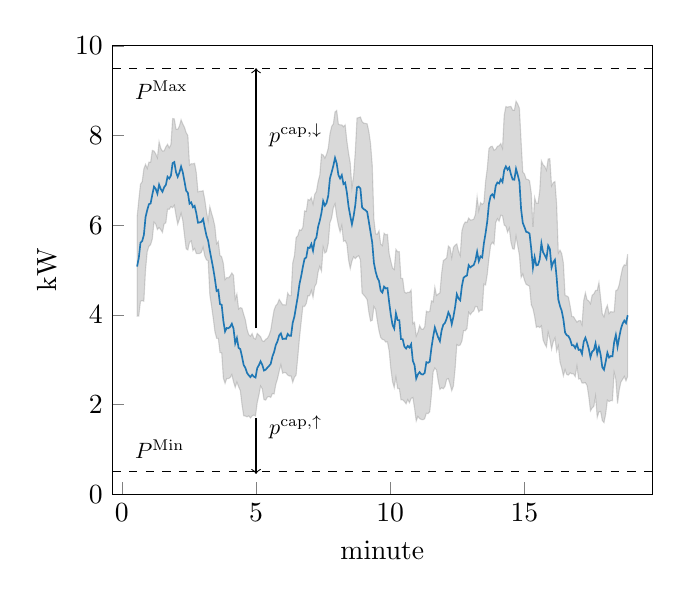
\begin{tikzpicture}

\definecolor{gray}{RGB}{128,128,128}
\definecolor{steelblue31119180}{RGB}{31,119,180}

\begin{axis}[
tick pos=left,
unbounded coords=jump,
xlabel={minute},
xmin=-0.346730961767435, xmax=19.7636648207438,
ylabel={kW},
ymin=0, ymax=10
]
\path [draw=gray, fill=gray, opacity=0.3]
(axis cs:0.567377937437621,6.18166486218385)
--(axis cs:0.567377937437621,3.96936101541136)
--(axis cs:0.630419930486246,3.97344638912022)
--(axis cs:0.693461923534871,4.30036914306906)
--(axis cs:0.756503916583495,4.31741647621636)
--(axis cs:0.81954590963212,4.30299042821583)
--(axis cs:0.882587902680744,5.00350797758454)
--(axis cs:0.945629895729369,5.40899753115722)
--(axis cs:1.00867188877799,5.52701107787508)
--(axis cs:1.07171388182662,5.56496784547894)
--(axis cs:1.13475587487524,5.69407386555207)
--(axis cs:1.19779786792387,6.06778541406991)
--(axis cs:1.26083986097249,6.02365541375591)
--(axis cs:1.32388185402112,5.90201403941722)
--(axis cs:1.38692384706974,5.94487201436298)
--(axis cs:1.44996584011837,5.8977241699591)
--(axis cs:1.51300783316699,5.83825427565187)
--(axis cs:1.57604982621562,6.03248892921176)
--(axis cs:1.63909181926424,6.04913622035933)
--(axis cs:1.70213381231286,6.35628893762452)
--(axis cs:1.76517580536149,6.353961367198)
--(axis cs:1.82821779841011,6.41393222082618)
--(axis cs:1.89125979145874,6.38877433034896)
--(axis cs:1.95430178450736,6.44439733098413)
--(axis cs:2.01734377755599,6.22203098681913)
--(axis cs:2.08038577060461,6.01995198790788)
--(axis cs:2.14342776365324,6.12973356489876)
--(axis cs:2.20646975670186,6.26312476393792)
--(axis cs:2.26951174975049,6.10495121066727)
--(axis cs:2.33255374279911,5.77408655675871)
--(axis cs:2.39559573584774,5.47213570668075)
--(axis cs:2.45863772889636,5.44633838168987)
--(axis cs:2.52167972194498,5.6185505171451)
--(axis cs:2.58472171499361,5.64806121388669)
--(axis cs:2.64776370804223,5.43239272623858)
--(axis cs:2.71080570109086,5.47990388658275)
--(axis cs:2.77384769413948,5.36728927384578)
--(axis cs:2.83688968718811,5.36465502013929)
--(axis cs:2.89993168023673,5.36800251172111)
--(axis cs:2.96297367328536,5.39343558806987)
--(axis cs:3.02601566633398,5.50375572043972)
--(axis cs:3.08905765938261,5.31492630358328)
--(axis cs:3.15209965243123,5.22525646595247)
--(axis cs:3.21514164547985,5.20719149001088)
--(axis cs:3.27818363852848,4.44303275826049)
--(axis cs:3.3412256315771,4.19335380135255)
--(axis cs:3.40426762462573,3.92254591850244)
--(axis cs:3.46730961767435,3.6241034940258)
--(axis cs:3.53035161072298,3.47568305900498)
--(axis cs:3.5933936037716,3.47189457505862)
--(axis cs:3.65643559682023,3.15697215357351)
--(axis cs:3.71947758986885,3.15334437213519)
--(axis cs:3.78251958291748,2.5827839601311)
--(axis cs:3.8455615759661,2.47037795237786)
--(axis cs:3.90860356901473,2.57877757449341)
--(axis cs:3.97164556206335,2.57586614244848)
--(axis cs:4.03468755511197,2.60093565014967)
--(axis cs:4.0977295481606,2.66629035345775)
--(axis cs:4.16077154120922,2.50514360333662)
--(axis cs:4.22381353425785,2.38051940985129)
--(axis cs:4.28685552730647,2.49965437400856)
--(axis cs:4.3498975203551,2.39527391236753)
--(axis cs:4.41293951340372,2.31191369611713)
--(axis cs:4.47598150645235,1.99566344493136)
--(axis cs:4.53902349950097,1.74838021430041)
--(axis cs:4.6020654925496,1.7412583877123)
--(axis cs:4.66510748559822,1.72430406041548)
--(axis cs:4.72814947864685,1.74583798813789)
--(axis cs:4.79119147169547,1.69920645529924)
--(axis cs:4.85423346474409,1.74403977737467)
--(axis cs:4.91727545779272,1.76329406992712)
--(axis cs:4.98031745084134,1.74283609797831)
--(axis cs:5.04335944388997,2.03658555657295)
--(axis cs:5.10640143693859,2.2074083992948)
--(axis cs:5.16944342998722,2.41130755001176)
--(axis cs:5.23248542303584,2.34711814331545)
--(axis cs:5.29552741608447,2.10806403938627)
--(axis cs:5.35856940913309,2.09742800525492)
--(axis cs:5.42161140218172,2.16324012037483)
--(axis cs:5.48465339523034,2.17857505019042)
--(axis cs:5.54769538827897,2.15632917926649)
--(axis cs:5.61073738132759,2.24385095243216)
--(axis cs:5.67377937437622,2.23548186272026)
--(axis cs:5.73682136742484,2.44772349001024)
--(axis cs:5.79986336047346,2.57135621790826)
--(axis cs:5.86290535352209,2.73867960447763)
--(axis cs:5.92594734657071,2.88535870068725)
--(axis cs:5.98898933961934,2.69515009339781)
--(axis cs:6.05203133266796,2.71276517998775)
--(axis cs:6.11507332571659,2.7061617189873)
--(axis cs:6.17811531876521,2.65621489830161)
--(axis cs:6.24115731181384,2.63446332445777)
--(axis cs:6.30419930486246,2.63458134652472)
--(axis cs:6.36724129791109,2.49301021525772)
--(axis cs:6.43028329095971,2.60633779805416)
--(axis cs:6.49332528400833,2.65705654962646)
--(axis cs:6.55636727705696,3.05697691966238)
--(axis cs:6.61940927010558,3.48128301732453)
--(axis cs:6.68245126315421,3.84226145976166)
--(axis cs:6.74549325620283,4.18996683698144)
--(axis cs:6.80853524925146,4.18527361227889)
--(axis cs:6.87157724230008,4.2519817382919)
--(axis cs:6.93461923534871,4.42481458609258)
--(axis cs:6.99766122839733,4.4258987984519)
--(axis cs:7.06070322144596,4.54320093296833)
--(axis cs:7.12374521449458,4.38928807396806)
--(axis cs:7.18678720754321,4.6313541496724)
--(axis cs:7.24982920059183,4.69751860727535)
--(axis cs:7.31287119364045,4.95509043031014)
--(axis cs:7.37591318668908,5.07949382909876)
--(axis cs:7.4389551797377,4.97421718464399)
--(axis cs:7.50199717278633,5.50980336792573)
--(axis cs:7.56503916583495,5.37687306320469)
--(axis cs:7.62808115888358,5.41231696205123)
--(axis cs:7.6911231519322,5.59061487061282)
--(axis cs:7.75416514498083,6.05282561759393)
--(axis cs:7.81720713802945,6.15803874106396)
--(axis cs:7.88024913107808,6.38974474868414)
--(axis cs:7.9432911241267,6.47581981501566)
--(axis cs:8.00633311717533,6.19312857192594)
--(axis cs:8.06937511022395,5.99032542301435)
--(axis cs:8.13241710327257,5.84690879486669)
--(axis cs:8.1954590963212,5.99125878169752)
--(axis cs:8.25850108936982,5.6378191069097)
--(axis cs:8.32154308241845,5.65603880255992)
--(axis cs:8.38458507546707,5.57602927706925)
--(axis cs:8.4476270685157,5.22378837321204)
--(axis cs:8.51066906156432,5.02994081346826)
--(axis cs:8.57371105461295,5.19545288456707)
--(axis cs:8.63675304766157,5.29453047160256)
--(axis cs:8.6997950407102,5.25273221675318)
--(axis cs:8.76283703375882,5.2955995922863)
--(axis cs:8.82587902680745,5.31695199442623)
--(axis cs:8.88892101985607,5.22574839036865)
--(axis cs:8.9519630129047,4.48219030603422)
--(axis cs:9.01500500595332,4.44071876033423)
--(axis cs:9.07804699900194,4.39519623267719)
--(axis cs:9.14108899205057,4.33643098080271)
--(axis cs:9.20413098509919,4.05786035244679)
--(axis cs:9.26717297814782,3.85947001724454)
--(axis cs:9.33021497119644,3.87835825199927)
--(axis cs:9.39325696424507,4.18408542702962)
--(axis cs:9.45629895729369,4.12145510572921)
--(axis cs:9.51934095034232,3.86269070874271)
--(axis cs:9.58238294339094,3.64231865536413)
--(axis cs:9.64542493643956,3.49264442780424)
--(axis cs:9.70846692948819,3.45052566831293)
--(axis cs:9.77150892253681,3.44018003861832)
--(axis cs:9.83455091558544,3.39258911540373)
--(axis cs:9.89759290863406,3.39593018604691)
--(axis cs:9.96063490168269,3.19289643440917)
--(axis cs:10.0236768947313,2.79225701479243)
--(axis cs:10.0867188877799,2.50651412900804)
--(axis cs:10.1497608808286,2.3758988549226)
--(axis cs:10.2128028738772,2.6060263224822)
--(axis cs:10.2758448669258,2.3552556588953)
--(axis cs:10.3388868599744,2.35490857058003)
--(axis cs:10.4019288530231,2.10243257991686)
--(axis cs:10.4649708460717,2.10193732162844)
--(axis cs:10.5280128391203,2.06968774422456)
--(axis cs:10.5910548321689,2.01425708515634)
--(axis cs:10.6540968252176,2.10871952850238)
--(axis cs:10.7171388182662,2.04004955654141)
--(axis cs:10.7801808113148,2.13489800722695)
--(axis cs:10.8432228043634,2.15400259856434)
--(axis cs:10.9062647974121,1.91851811754127)
--(axis cs:10.9693067904607,1.63055958878258)
--(axis cs:11.0323487835093,1.73295766885185)
--(axis cs:11.0953907765579,1.68418239107452)
--(axis cs:11.1584327696066,1.6656096035353)
--(axis cs:11.2214747626552,1.65913737564199)
--(axis cs:11.2845167557038,1.68061311950504)
--(axis cs:11.3475587487524,1.8042938430006)
--(axis cs:11.4106007418011,1.79529502973798)
--(axis cs:11.4736427348497,1.83554593412024)
--(axis cs:11.5366847278983,2.21667475067341)
--(axis cs:11.5997267209469,2.72574162512461)
--(axis cs:11.6627687139956,2.81316484993346)
--(axis cs:11.7258107070442,2.7677823799969)
--(axis cs:11.7888527000928,2.52299594781739)
--(axis cs:11.8518946931414,2.33607528479337)
--(axis cs:11.9149366861901,2.37400307396125)
--(axis cs:11.9779786792387,2.35056244345395)
--(axis cs:12.0410206722873,2.400584191414)
--(axis cs:12.1040626653359,2.56174616571575)
--(axis cs:12.1671046583845,2.5758580866907)
--(axis cs:12.2301466514332,2.45131592151387)
--(axis cs:12.2931886444818,2.3076832899623)
--(axis cs:12.3562306375304,2.411678967237)
--(axis cs:12.419272630579,2.79674055629717)
--(axis cs:12.4823146236277,3.33655488788582)
--(axis cs:12.5453566166763,3.31167800745318)
--(axis cs:12.6083986097249,3.32641279093409)
--(axis cs:12.6714406027735,3.41026503291946)
--(axis cs:12.7344825958222,3.64764885586557)
--(axis cs:12.7975245888708,3.64540211358649)
--(axis cs:12.8605665819194,3.69241695934241)
--(axis cs:12.923608574968,4.05615240058902)
--(axis cs:12.9866505680167,4.00244701358177)
--(axis cs:13.0496925610653,4.05724066632932)
--(axis cs:13.1127345541139,4.08566880255474)
--(axis cs:13.1757765471625,4.18769051262905)
--(axis cs:13.2388185402112,4.18225650384859)
--(axis cs:13.3018605332598,4.06442382931898)
--(axis cs:13.3649025263084,4.10545681382759)
--(axis cs:13.427944519357,4.09802550660088)
--(axis cs:13.4909865124057,4.68495189446625)
--(axis cs:13.5540285054543,4.66541162771275)
--(axis cs:13.6170704985029,4.90181765288723)
--(axis cs:13.6801124915515,5.25582684778678)
--(axis cs:13.7431544846002,5.55408004460812)
--(axis cs:13.8061964776488,5.61753770657008)
--(axis cs:13.8692384706974,5.57474070245099)
--(axis cs:13.932280463746,6.05896010868592)
--(axis cs:13.9953224567947,6.14393207160121)
--(axis cs:14.0583644498433,6.08808079057294)
--(axis cs:14.1214064428919,6.22182393899643)
--(axis cs:14.1844484359405,6.21125513143774)
--(axis cs:14.2474904289892,6.00224652229704)
--(axis cs:14.3105324220378,5.97449319421745)
--(axis cs:14.3735744150864,5.841737532699)
--(axis cs:14.436616408135,5.93226370423007)
--(axis cs:14.4996584011837,5.61805098213557)
--(axis cs:14.5627003942323,5.47055167624038)
--(axis cs:14.6257423872809,5.46538292978251)
--(axis cs:14.6887843803295,5.74895114384429)
--(axis cs:14.7518263733782,5.5370812318468)
--(axis cs:14.8148683664268,5.32914681504781)
--(axis cs:14.8779103594754,4.83627109755209)
--(axis cs:14.940952352524,4.91183878796624)
--(axis cs:15.0039943455727,4.76930435731819)
--(axis cs:15.0670363386213,4.67869216289833)
--(axis cs:15.1300783316699,4.65900273904369)
--(axis cs:15.1931203247185,4.6343516238587)
--(axis cs:15.2561623177672,4.22269773453472)
--(axis cs:15.3192043108158,4.13874176617292)
--(axis cs:15.3822463038644,3.95917694570799)
--(axis cs:15.445288296913,3.71811503548311)
--(axis cs:15.5083302899617,3.74287878414705)
--(axis cs:15.5713722830103,3.71494492978732)
--(axis cs:15.6344142760589,3.75415884472509)
--(axis cs:15.6974562691075,3.43924667764085)
--(axis cs:15.7604982621562,3.3493287500099)
--(axis cs:15.8235402552048,3.28049992560553)
--(axis cs:15.8865822482534,3.60998100176738)
--(axis cs:15.949624241302,3.45911159666157)
--(axis cs:16.0126662343507,3.23374257568519)
--(axis cs:16.0757082273993,3.39694791111434)
--(axis cs:16.1387502204479,3.48328291437016)
--(axis cs:16.2017922134965,3.19058179574846)
--(axis cs:16.2648342065451,3.30983102076004)
--(axis cs:16.3278761995938,2.94484774903207)
--(axis cs:16.3909181926424,2.80891497346496)
--(axis cs:16.453960185691,2.63753820934079)
--(axis cs:16.5170021787396,2.77591650439555)
--(axis cs:16.5800441717883,2.66705777557643)
--(axis cs:16.6430861648369,2.65578577464367)
--(axis cs:16.7061281578855,2.7059178178044)
--(axis cs:16.7691701509341,2.6829852023348)
--(axis cs:16.8322121439828,2.68099135008852)
--(axis cs:16.8952541370314,2.62331094681754)
--(axis cs:16.95829613008,2.85531069880462)
--(axis cs:17.0213381231286,2.56754997041599)
--(axis cs:17.0843801161773,2.57434592702845)
--(axis cs:17.1474221092259,2.47927165561288)
--(axis cs:17.2104641022745,2.47811083678863)
--(axis cs:17.2735060953231,2.48605830271505)
--(axis cs:17.3365480883718,2.42369659481194)
--(axis cs:17.3995900814204,2.17886017799649)
--(axis cs:17.462632074469,1.85653565448379)
--(axis cs:17.5256740675176,1.92186953613526)
--(axis cs:17.5887160605663,1.95635493455709)
--(axis cs:17.6517580536149,2.1806630106001)
--(axis cs:17.7148000466635,1.71419328995482)
--(axis cs:17.7778420397121,1.83457373884102)
--(axis cs:17.8408840327608,1.84515087057149)
--(axis cs:17.9039260258094,1.64073560132732)
--(axis cs:17.966968018858,1.59502259856721)
--(axis cs:18.0300100119066,1.7855599106726)
--(axis cs:18.0930520049553,2.0972455732254)
--(axis cs:18.1560939980039,2.0655252886156)
--(axis cs:18.2191359910525,2.08636653170534)
--(axis cs:18.2821779841011,2.08363284416694)
--(axis cs:18.3452199771498,2.71548071811183)
--(axis cs:18.4082619701984,2.55605524021846)
--(axis cs:18.471303963247,2.01978139144438)
--(axis cs:18.5343459562956,2.3210267694918)
--(axis cs:18.5973879493443,2.49825407851481)
--(axis cs:18.6604299423929,2.55933491112866)
--(axis cs:18.7234719354415,2.62499856208103)
--(axis cs:18.7865139284901,2.5265990814035)
--(axis cs:18.8495559215388,2.62672736938327)
--(axis cs:18.8495559215388,5.35457975662859)
--(axis cs:18.8495559215388,5.35457975662859)
--(axis cs:18.7865139284901,5.10356865520516)
--(axis cs:18.7234719354415,5.11465600995625)
--(axis cs:18.6604299423929,5.04670534693652)
--(axis cs:18.5973879493443,4.87204886899746)
--(axis cs:18.5343459562956,4.67413712653839)
--(axis cs:18.471303963247,4.55536635865353)
--(axis cs:18.4082619701984,4.54388358599681)
--(axis cs:18.3452199771498,4.06450211300715)
--(axis cs:18.2821779841011,4.06328827863933)
--(axis cs:18.2191359910525,4.07086077977646)
--(axis cs:18.1560939980039,4.02719663344008)
--(axis cs:18.0930520049553,4.21267525663078)
--(axis cs:18.0300100119066,4.12015098625053)
--(axis cs:17.966968018858,3.95427581685924)
--(axis cs:17.9039260258094,4.01943481860276)
--(axis cs:17.8408840327608,4.37969749260543)
--(axis cs:17.7778420397121,4.71992563991477)
--(axis cs:17.7148000466635,4.54675854643261)
--(axis cs:17.6517580536149,4.54355870392897)
--(axis cs:17.5887160605663,4.46441790450028)
--(axis cs:17.5256740675176,4.437231819227)
--(axis cs:17.462632074469,4.24721992282555)
--(axis cs:17.3995900814204,4.31039950439255)
--(axis cs:17.3365480883718,4.33630074318893)
--(axis cs:17.2735060953231,4.49068577419421)
--(axis cs:17.2104641022745,4.31622925190862)
--(axis cs:17.1474221092259,3.77686936611446)
--(axis cs:17.0843801161773,3.87332530193415)
--(axis cs:17.0213381231286,3.86726427510923)
--(axis cs:16.95829613008,3.83661969437702)
--(axis cs:16.8952541370314,3.89323679477223)
--(axis cs:16.8322121439828,3.95818859969472)
--(axis cs:16.7691701509341,3.96123166033146)
--(axis cs:16.7061281578855,4.19659059039086)
--(axis cs:16.6430861648369,4.3922375654297)
--(axis cs:16.5800441717883,4.42088776556141)
--(axis cs:16.5170021787396,4.42953031480533)
--(axis cs:16.453960185691,5.15637573044096)
--(axis cs:16.3909181926424,5.36752676523488)
--(axis cs:16.3278761995938,5.44337832572932)
--(axis cs:16.2648342065451,5.37561191942613)
--(axis cs:16.2017922134965,6.477041155664)
--(axis cs:16.1387502204479,6.97174708404889)
--(axis cs:16.0757082273993,6.9491858415767)
--(axis cs:16.0126662343507,6.87690298372766)
--(axis cs:15.949624241302,7.48181910117281)
--(axis cs:15.8865822482534,7.47541402875201)
--(axis cs:15.8235402552048,7.22614087354199)
--(axis cs:15.7604982621562,7.30795726514729)
--(axis cs:15.6974562691075,7.34745353688197)
--(axis cs:15.6344142760589,7.43337328155885)
--(axis cs:15.5713722830103,6.76137312902249)
--(axis cs:15.5083302899617,6.48782443354453)
--(axis cs:15.445288296913,6.48712348933014)
--(axis cs:15.3822463038644,6.61617539767449)
--(axis cs:15.3192043108158,5.95934348751698)
--(axis cs:15.2561623177672,6.71539109014808)
--(axis cs:15.1931203247185,6.98883189647299)
--(axis cs:15.1300783316699,7.02077071757537)
--(axis cs:15.0670363386213,7.02358213495139)
--(axis cs:15.0039943455727,7.14123875054786)
--(axis cs:14.940952352524,7.18537910494122)
--(axis cs:14.8779103594754,7.87265922246595)
--(axis cs:14.8148683664268,8.60682709317454)
--(axis cs:14.7518263733782,8.70300652906748)
--(axis cs:14.6887843803295,8.76465476914033)
--(axis cs:14.6257423872809,8.55955682985371)
--(axis cs:14.5627003942323,8.56594139192577)
--(axis cs:14.4996584011837,8.64708248330412)
--(axis cs:14.436616408135,8.64267787912975)
--(axis cs:14.3735744150864,8.63104575366701)
--(axis cs:14.3105324220378,8.64548713120545)
--(axis cs:14.2474904289892,8.45145216108748)
--(axis cs:14.1844484359405,7.71441479072257)
--(axis cs:14.1214064428919,7.82079264795362)
--(axis cs:14.0583644498433,7.76955247380292)
--(axis cs:13.9953224567947,7.75778182560015)
--(axis cs:13.932280463746,7.69280547782909)
--(axis cs:13.8692384706974,7.6710753001372)
--(axis cs:13.8061964776488,7.75842524875786)
--(axis cs:13.7431544846002,7.75191377464573)
--(axis cs:13.6801124915515,7.70689905124487)
--(axis cs:13.6170704985029,7.26571166052962)
--(axis cs:13.5540285054543,6.97749753382679)
--(axis cs:13.4909865124057,6.50188168423864)
--(axis cs:13.427944519357,6.46187229598731)
--(axis cs:13.3649025263084,6.50268459604729)
--(axis cs:13.3018605332598,6.32752167705116)
--(axis cs:13.2388185402112,6.62806793047447)
--(axis cs:13.1757765471625,6.2398625632339)
--(axis cs:13.1127345541139,6.13362259207894)
--(axis cs:13.0496925610653,6.11809083084867)
--(axis cs:12.9866505680167,6.11395206378882)
--(axis cs:12.923608574968,6.1580429715405)
--(axis cs:12.8605665819194,6.05855277905852)
--(axis cs:12.7975245888708,6.07156193819638)
--(axis cs:12.7344825958222,6.00602241541999)
--(axis cs:12.6714406027735,5.87209969435715)
--(axis cs:12.6083986097249,5.32038680375972)
--(axis cs:12.5453566166763,5.41702678553876)
--(axis cs:12.4823146236277,5.58176666369775)
--(axis cs:12.419272630579,5.55452092267111)
--(axis cs:12.3562306375304,5.50733842952364)
--(axis cs:12.2931886444818,5.27561557415291)
--(axis cs:12.2301466514332,5.49867797284539)
--(axis cs:12.1671046583845,5.53564352845668)
--(axis cs:12.1040626653359,5.26779216888733)
--(axis cs:12.0410206722873,5.23671105895476)
--(axis cs:11.9779786792387,5.2087614743483)
--(axis cs:11.9149366861901,4.92394164344543)
--(axis cs:11.8518946931414,4.48631326049891)
--(axis cs:11.7888527000928,4.46514169805785)
--(axis cs:11.7258107070442,4.43281866354911)
--(axis cs:11.6627687139956,4.61743941584526)
--(axis cs:11.5997267209469,4.28792180344055)
--(axis cs:11.5366847278983,4.31318022626334)
--(axis cs:11.4736427348497,4.07632589374662)
--(axis cs:11.4106007418011,4.06377997378538)
--(axis cs:11.3475587487524,4.08323626726787)
--(axis cs:11.2845167557038,3.72675310816805)
--(axis cs:11.2214747626552,3.67668719711129)
--(axis cs:11.1584327696066,3.68432156577277)
--(axis cs:11.0953907765579,3.75926010711575)
--(axis cs:11.0323487835093,3.61073910936081)
--(axis cs:10.9693067904607,3.52658866854417)
--(axis cs:10.9062647974121,3.83377974604342)
--(axis cs:10.8432228043634,3.79780063014933)
--(axis cs:10.7801808113148,4.55430518124831)
--(axis cs:10.7171388182662,4.49982532763056)
--(axis cs:10.6540968252176,4.50234817810973)
--(axis cs:10.5910548321689,4.48118869051546)
--(axis cs:10.5280128391203,4.51517988813942)
--(axis cs:10.4649708460717,4.81005540456859)
--(axis cs:10.4019288530231,4.8121708291403)
--(axis cs:10.3388868599744,5.40611491715658)
--(axis cs:10.2758448669258,5.40671293375523)
--(axis cs:10.2128028738772,5.46027290146165)
--(axis cs:10.1497608808286,5.00948725731778)
--(axis cs:10.0867188877799,5.04322356423389)
--(axis cs:10.0236768947313,5.19595229976629)
--(axis cs:9.96063490168269,5.36739568719899)
--(axis cs:9.89759290863406,5.79412820650933)
--(axis cs:9.83455091558544,5.78500794497034)
--(axis cs:9.77150892253681,5.81849796545678)
--(axis cs:9.70846692948819,5.54444757763506)
--(axis cs:9.64542493643956,5.58041493104084)
--(axis cs:9.58238294339094,5.87095541324995)
--(axis cs:9.51934095034232,5.7980021224282)
--(axis cs:9.45629895729369,5.80440554922189)
--(axis cs:9.39325696424507,6.12931049971949)
--(axis cs:9.33021497119644,7.34158896967502)
--(axis cs:9.26717297814782,7.8227115892379)
--(axis cs:9.20413098509919,8.09110497388025)
--(axis cs:9.14108899205057,8.2585926271438)
--(axis cs:9.07804699900194,8.27086446422967)
--(axis cs:9.01500500595332,8.27286866544587)
--(axis cs:8.9519630129047,8.30873524227611)
--(axis cs:8.88892101985607,8.41296033560557)
--(axis cs:8.82587902680745,8.40050090984576)
--(axis cs:8.76283703375882,8.38782226196934)
--(axis cs:8.6997950407102,7.65465621819623)
--(axis cs:8.63675304766157,7.11188546102187)
--(axis cs:8.57371105461295,6.84188072742058)
--(axis cs:8.51066906156432,7.38583495386274)
--(axis cs:8.4476270685157,7.60858260732916)
--(axis cs:8.38458507546707,7.88133701528036)
--(axis cs:8.32154308241845,8.23652461362219)
--(axis cs:8.25850108936982,8.19462837046459)
--(axis cs:8.1954590963212,8.23784601720616)
--(axis cs:8.13241710327257,8.23695058342243)
--(axis cs:8.06937511022395,8.24889241293588)
--(axis cs:8.00633311717533,8.55810614451799)
--(axis cs:7.9432911241267,8.52373922492956)
--(axis cs:7.88024913107808,8.25613541274214)
--(axis cs:7.81720713802945,8.20091222743021)
--(axis cs:7.75416514498083,8.03322923434425)
--(axis cs:7.6911231519322,7.71717866384189)
--(axis cs:7.62808115888358,7.58027422168324)
--(axis cs:7.56503916583495,7.49561260373038)
--(axis cs:7.50199717278633,7.56465162980608)
--(axis cs:7.4389551797377,7.58198641669796)
--(axis cs:7.37591318668908,7.1202490472343)
--(axis cs:7.31287119364045,6.97245448697429)
--(axis cs:7.24982920059183,6.74945278528487)
--(axis cs:7.18678720754321,6.68630569104179)
--(axis cs:7.12374521449458,6.47037154930805)
--(axis cs:7.06070322144596,6.61521994493979)
--(axis cs:6.99766122839733,6.5565379716877)
--(axis cs:6.93461923534871,6.57244931814677)
--(axis cs:6.87157724230008,6.30442923773725)
--(axis cs:6.80853524925146,6.31762260905189)
--(axis cs:6.74549325620283,5.95251637109349)
--(axis cs:6.68245126315421,5.88464923862517)
--(axis cs:6.61940927010558,5.89669096702679)
--(axis cs:6.55636727705696,5.76263905802055)
--(axis cs:6.49332528400833,5.72148384146649)
--(axis cs:6.43028329095971,5.31708908515244)
--(axis cs:6.36724129791109,5.15758610129024)
--(axis cs:6.30419930486246,4.42707644476656)
--(axis cs:6.24115731181384,4.42842089460486)
--(axis cs:6.17811531876521,4.4871791362882)
--(axis cs:6.11507332571659,4.21891472830644)
--(axis cs:6.05203133266796,4.22406437148649)
--(axis cs:5.98898933961934,4.22396843629301)
--(axis cs:5.92594734657071,4.28440420325753)
--(axis cs:5.86290535352209,4.34532076037739)
--(axis cs:5.79986336047346,4.24706224087863)
--(axis cs:5.73682136742484,4.20344773516475)
--(axis cs:5.67377937437622,4.11087093770172)
--(axis cs:5.61073738132759,3.89562974174326)
--(axis cs:5.54769538827897,3.65834508965189)
--(axis cs:5.48465339523034,3.54144561337847)
--(axis cs:5.42161140218172,3.47690921767769)
--(axis cs:5.35856940913309,3.45286541881504)
--(axis cs:5.29552741608447,3.40644824193479)
--(axis cs:5.23248542303584,3.41963741555389)
--(axis cs:5.16944342998722,3.51340098489306)
--(axis cs:5.10640143693859,3.54695002902822)
--(axis cs:5.04335944388997,3.58414616418799)
--(axis cs:4.98031745084134,3.45800077120311)
--(axis cs:4.91727545779272,3.47818108434613)
--(axis cs:4.85423346474409,3.58187937786535)
--(axis cs:4.79119147169547,3.52261964720559)
--(axis cs:4.72814947864685,3.55582658514886)
--(axis cs:4.66510748559822,3.67886784776418)
--(axis cs:4.6020654925496,3.89076963080303)
--(axis cs:4.53902349950097,4.01252303722714)
--(axis cs:4.47598150645235,4.14719899033398)
--(axis cs:4.41293951340372,4.15903899364169)
--(axis cs:4.3498975203551,4.12813010402487)
--(axis cs:4.28685552730647,4.46532982036871)
--(axis cs:4.22381353425785,4.34648771187588)
--(axis cs:4.16077154120922,4.87910854418792)
--(axis cs:4.0977295481606,4.9341295141979)
--(axis cs:4.03468755511197,4.86448253573226)
--(axis cs:3.97164556206335,4.82409577193263)
--(axis cs:3.90860356901473,4.83042602386556)
--(axis cs:3.8455615759661,4.78433174020021)
--(axis cs:3.78251958291748,5.14478882583466)
--(axis cs:3.71947758986885,5.29422719811486)
--(axis cs:3.65643559682023,5.32591262474865)
--(axis cs:3.5933936037716,5.63697048742318)
--(axis cs:3.53035161072298,5.58604703769755)
--(axis cs:3.46730961767435,5.97251314243477)
--(axis cs:3.40426762462573,6.14028581326012)
--(axis cs:3.3412256315771,6.27042620611646)
--(axis cs:3.27818363852848,6.41186320964337)
--(axis cs:3.21514164547985,6.09396988802331)
--(axis cs:3.15209965243123,6.30759914139846)
--(axis cs:3.08905765938261,6.57533951150494)
--(axis cs:3.02601566633398,6.76943577418586)
--(axis cs:2.96297367328536,6.75556262874277)
--(axis cs:2.89993168023673,6.75499567834843)
--(axis cs:2.83688968718811,6.74292131775476)
--(axis cs:2.77384769413948,7.17071328058774)
--(axis cs:2.71080570109086,7.37993484497515)
--(axis cs:2.64776370804223,7.36767255930127)
--(axis cs:2.58472171499361,7.36852405441932)
--(axis cs:2.52167972194498,7.33764512593136)
--(axis cs:2.45863772889636,8.00008428126556)
--(axis cs:2.39559573584774,8.0626456460787)
--(axis cs:2.33255374279911,8.18466075151602)
--(axis cs:2.26951174975049,8.25560087763157)
--(axis cs:2.20646975670186,8.3499687784209)
--(axis cs:2.14342776365324,8.20992651806108)
--(axis cs:2.08038577060461,8.13537247155989)
--(axis cs:2.01734377755599,8.14181273837627)
--(axis cs:1.95430178450736,8.36989838425807)
--(axis cs:1.89125979145874,8.37740914543832)
--(axis cs:1.82821779841011,7.79525693949959)
--(axis cs:1.76517580536149,7.72480800316175)
--(axis cs:1.70213381231286,7.80286329673218)
--(axis cs:1.63909181926424,7.74456409117588)
--(axis cs:1.57604982621562,7.65830886857741)
--(axis cs:1.51300783316699,7.65139478555581)
--(axis cs:1.44996584011837,7.7120286888103)
--(axis cs:1.38692384706974,7.86251918765089)
--(axis cs:1.32388185402112,7.50317546067804)
--(axis cs:1.26083986097249,7.59283075596556)
--(axis cs:1.19779786792387,7.65172084907224)
--(axis cs:1.13475587487524,7.66728127470102)
--(axis cs:1.07171388182662,7.40378087612505)
--(axis cs:1.00867188877799,7.40658808861352)
--(axis cs:0.945629895729369,7.26651531303412)
--(axis cs:0.882587902680744,7.35535513089669)
--(axis cs:0.81954590963212,7.25581187628329)
--(axis cs:0.756503916583495,6.96859258847075)
--(axis cs:0.693461923534871,6.9144349961022)
--(axis cs:0.630419930486246,6.56308619227699)
--(axis cs:0.567377937437621,6.18166486218385)
--cycle;

\addplot [semithick, steelblue31119180]
table {%
0 nan
0.0630419930486246 nan
0.126083986097249 nan
0.189125979145874 nan
0.252167972194498 nan
0.315209965243123 nan
0.378251958291748 nan
0.441293951340372 nan
0.504335944388997 nan
0.567377937437621 5.0755129387976
0.630419930486246 5.2682662906986
0.693461923534871 5.60740206958563
0.756503916583495 5.64300453234356
0.81954590963212 5.77940115224956
0.882587902680744 6.17943155424062
0.945629895729369 6.33775642209567
1.00867188877799 6.4667995832443
1.07171388182662 6.484374360802
1.13475587487524 6.68067757012654
1.19779786792387 6.85975313157107
1.26083986097249 6.80824308486074
1.32388185402112 6.70259475004763
1.38692384706974 6.90369560100693
1.44996584011837 6.8048764293847
1.51300783316699 6.74482453060384
1.57604982621562 6.84539889889459
1.63909181926424 6.89685015576761
1.70213381231286 7.07957611717835
1.76517580536149 7.03938468517988
1.82821779841011 7.10459458016289
1.89125979145874 7.38309173789364
1.95430178450736 7.4071478576211
2.01734377755599 7.1819218625977
2.08038577060461 7.07766222973388
2.14342776365324 7.16983004147992
2.20646975670186 7.30654677117941
2.26951174975049 7.18027604414942
2.33255374279911 6.97937365413737
2.39559573584774 6.76739067637972
2.45863772889636 6.72321133147772
2.52167972194498 6.47809782153823
2.58472171499361 6.50829263415301
2.64776370804223 6.40003264276992
2.71080570109086 6.42991936577895
2.77384769413948 6.26900127721676
2.83688968718811 6.05378816894703
2.89993168023673 6.06149909503477
2.96297367328536 6.07449910840632
3.02601566633398 6.13659574731279
3.08905765938261 5.94513290754411
3.15209965243123 5.76642780367546
3.21514164547985 5.65058068901709
3.27818363852848 5.42744798395193
3.3412256315771 5.2318900037345
3.40426762462573 5.03141586588128
3.46730961767435 4.79830831823029
3.53035161072298 4.53086504835126
3.5933936037716 4.5544325312409
3.65643559682023 4.24144238916108
3.71947758986885 4.22378578512502
3.78251958291748 3.86378639298288
3.8455615759661 3.62735484628903
3.90860356901473 3.70460179917948
3.97164556206335 3.69998095719056
4.03468755511197 3.73270909294096
4.0977295481606 3.80020993382782
4.16077154120922 3.69212607376227
4.22381353425785 3.36350356086358
4.28685552730647 3.48249209718863
4.3498975203551 3.2617020081962
4.41293951340372 3.23547634487941
4.47598150645235 3.07143121763267
4.53902349950097 2.88045162576377
4.6020654925496 2.81601400925766
4.66510748559822 2.70158595408983
4.72814947864685 2.65083228664338
4.79119147169547 2.61091305125241
4.85423346474409 2.66295957762001
4.91727545779272 2.62073757713663
4.98031745084134 2.60041843459071
5.04335944388997 2.81036586038047
5.10640143693859 2.87717921416151
5.16944342998722 2.96235426745241
5.23248542303584 2.88337777943467
5.29552741608447 2.75725614066053
5.35856940913309 2.77514671203498
5.42161140218172 2.82007466902626
5.48465339523034 2.86001033178444
5.54769538827897 2.90733713445919
5.61073738132759 3.06974034708771
5.67377937437622 3.17317640021099
5.73682136742484 3.3255856125875
5.79986336047346 3.40920922939344
5.86290535352209 3.54200018242751
5.92594734657071 3.58488145197239
5.98898933961934 3.45955926484541
6.05203133266796 3.46841477573712
6.11507332571659 3.46253822364687
6.17811531876521 3.5716970172949
6.24115731181384 3.53144210953131
6.30419930486246 3.53082889564564
6.36724129791109 3.82529815827398
6.43028329095971 3.9617134416033
6.49332528400833 4.18927019554648
6.55636727705696 4.40980798884147
6.61940927010558 4.68898699217566
6.68245126315421 4.86345534919341
6.74549325620283 5.07124160403747
6.80853524925146 5.25144811066539
6.87157724230008 5.27820548801457
6.93461923534871 5.49863195211967
6.99766122839733 5.4912183850698
7.06070322144596 5.57921043895406
7.12374521449458 5.42982981163806
7.18678720754321 5.6588299203571
7.24982920059183 5.72348569628011
7.31287119364045 5.96377245864222
7.37591318668908 6.09987143816653
7.4389551797377 6.27810180067098
7.50199717278633 6.53722749886591
7.56503916583495 6.43624283346754
7.62808115888358 6.49629559186723
7.6911231519322 6.65389676722735
7.75416514498083 7.04302742596909
7.81720713802945 7.17947548424709
7.88024913107808 7.32294008071314
7.9432911241267 7.49977951997261
8.00633311717533 7.37561735822196
8.06937511022395 7.11960891797511
8.13241710327257 7.04192968914456
8.1954590963212 7.11455239945184
8.25850108936982 6.91622373868714
8.32154308241845 6.94628170809105
8.38458507546707 6.72868314617481
8.4476270685157 6.4161854902706
8.51066906156432 6.2078878836655
8.57371105461295 6.01866680599383
8.63675304766157 6.20320796631222
8.6997950407102 6.45369421747471
8.76283703375882 6.84171092712782
8.82587902680745 6.85872645213599
8.88892101985607 6.81935436298711
8.9519630129047 6.39546277415516
9.01500500595332 6.35679371289005
9.07804699900194 6.33303034845343
9.14108899205057 6.29751180397325
9.20413098509919 6.07448266316352
9.26717297814782 5.84109080324122
9.33021497119644 5.60997361083714
9.39325696424507 5.15669796337455
9.45629895729369 4.96293032747555
9.51934095034232 4.83034641558545
9.58238294339094 4.75663703430704
9.64542493643956 4.53652967942254
9.70846692948819 4.49748662297399
9.77150892253681 4.62933900203755
9.83455091558544 4.58879853018704
9.89759290863406 4.59502919627812
9.96063490168269 4.28014606080408
10.0236768947313 3.99410465727936
10.0867188877799 3.77486884662097
10.1497608808286 3.69269305612019
10.2128028738772 4.03314961197192
10.2758448669258 3.88098429632527
10.3388868599744 3.88051174386831
10.4019288530231 3.45730170452858
10.4649708460717 3.45599636309851
10.5280128391203 3.29243381618199
10.5910548321689 3.2477228878359
10.6540968252176 3.30553385330605
10.7171388182662 3.26993744208598
10.7801808113148 3.34460159423763
10.8432228043634 2.97590161435684
10.9062647974121 2.87614893179235
10.9693067904607 2.57857412866337
11.0323487835093 2.67184838910633
11.0953907765579 2.72172124909513
11.1584327696066 2.67496558465404
11.2214747626552 2.66791228637664
11.2845167557038 2.70368311383654
11.3475587487524 2.94376505513424
11.4106007418011 2.92953750176168
11.4736427348497 2.95593591393343
11.5366847278983 3.26492748846838
11.5997267209469 3.50683171428258
11.6627687139956 3.71530213288936
11.7258107070442 3.600300521773
11.7888527000928 3.49406882293762
11.8518946931414 3.41119427264614
11.9149366861901 3.64897235870334
11.9779786792387 3.77966195890113
12.0410206722873 3.81864762518438
12.1040626653359 3.91476916730154
12.1671046583845 4.05575080757369
12.2301466514332 3.97499694717963
12.2931886444818 3.7916494320576
12.3562306375304 3.95950869838032
12.419272630579 4.17563073948414
12.4823146236277 4.45916077579179
12.5453566166763 4.36435239649597
12.6083986097249 4.3233997973469
12.6714406027735 4.64118236363831
12.7344825958222 4.82683563564278
12.7975245888708 4.85848202589144
12.8605665819194 4.87548486920046
12.923608574968 5.10709768606476
12.9866505680167 5.05819953868529
13.0496925610653 5.087665748589
13.1127345541139 5.10964569731684
13.1757765471625 5.21377653793147
13.2388185402112 5.40516221716153
13.3018605332598 5.19597275318507
13.3649025263084 5.30407070493744
13.427944519357 5.2799489012941
13.4909865124057 5.59341678935245
13.5540285054543 5.82145458076977
13.6170704985029 6.08376465670842
13.6801124915515 6.48136294951582
13.7431544846002 6.65299690962693
13.8061964776488 6.68798147766397
13.8692384706974 6.62290800129409
13.932280463746 6.8758827932575
13.9953224567947 6.95085694860068
14.0583644498433 6.92881663218793
14.1214064428919 7.02130829347503
14.1844484359405 6.96283496108015
14.2474904289892 7.22684934169226
14.3105324220378 7.30999016271145
14.3735744150864 7.236391643183
14.436616408135 7.28747079167991
14.4996584011837 7.13256673271984
14.5627003942323 7.01824653408307
14.6257423872809 7.01246987981811
14.6887843803295 7.25680295649231
14.7518263733782 7.12004388045714
14.8148683664268 6.96798695411118
14.8779103594754 6.35446516000902
14.940952352524 6.04860894645373
15.0039943455727 5.95527155393303
15.0670363386213 5.85113714892486
15.1300783316699 5.83988672830953
15.1931203247185 5.81159176016584
15.2561623177672 5.4690444123414
15.3192043108158 5.04904262684495
15.3822463038644 5.28767617169124
15.445288296913 5.10261926240663
15.5083302899617 5.11535160884579
15.5713722830103 5.2381590294049
15.6344142760589 5.59376606314197
15.6974562691075 5.39335010726141
15.7604982621562 5.32864300757859
15.8235402552048 5.25332039957376
15.8865822482534 5.54269751525969
15.949624241302 5.47046534891719
16.0126662343507 5.05532277970643
16.0757082273993 5.17306687634552
16.1387502204479 5.22751499920953
16.2017922134965 4.83381147570623
16.2648342065451 4.34272147009308
16.3278761995938 4.19411303738069
16.3909181926424 4.08822086934992
16.453960185691 3.89695696989088
16.5170021787396 3.60272340960044
16.5800441717883 3.54397277056892
16.6430861648369 3.52401167003668
16.7061281578855 3.45125420409763
16.7691701509341 3.32210843133313
16.8322121439828 3.31958997489162
16.8952541370314 3.25827387079489
16.95829613008 3.34596519659082
17.0213381231286 3.21740712276261
17.0843801161773 3.2238356144813
17.1474221092259 3.12807051086367
17.2104641022745 3.39717004434862
17.2735060953231 3.48837203845463
17.3365480883718 3.37999866900043
17.3995900814204 3.24462984119452
17.462632074469 3.05187778865467
17.5256740675176 3.17955067768113
17.5887160605663 3.21038641952869
17.6517580536149 3.36211085726453
17.7148000466635 3.13047591819372
17.7778420397121 3.27724968937789
17.8408840327608 3.11242418158846
17.9039260258094 2.83008520996504
17.966968018858 2.77464920771323
18.0300100119066 2.95285544846157
18.0930520049553 3.15496041492809
18.1560939980039 3.04636096102784
18.2191359910525 3.0786136557409
18.2821779841011 3.07346056140313
18.3452199771498 3.38999141555949
18.4082619701984 3.54996941310763
18.471303963247 3.28757387504896
18.5343459562956 3.49758194801509
18.5973879493443 3.68515147375613
18.6604299423929 3.80302012903259
18.7234719354415 3.86982728601864
18.7865139284901 3.81508386830433
18.8495559215388 3.99065356300593
};
\addplot [black, dashed]
table {%
-0.346730961767435 0.5
19.7636648207438 0.5
};
\addplot [black, dashed]
table {%
-0.346730961767435 9.5
19.7636648207438 9.5
};
\draw[->,draw=black] (axis cs:5,3.7) -- (axis cs:5,9.5);
\draw (axis cs:5.2,8) node[
  scale=0.8,
  anchor=west,
  text=black,
  rotate=0.0
]{$p^{\mathrm{cap},\downarrow}$};
\draw[->,draw=black] (axis cs:5,1.7) -- (axis cs:5,0.45);
\draw (axis cs:5.2,1.5) node[
  scale=0.8,
  anchor=west,
  text=black,
  rotate=0.0
]{$p^{\mathrm{cap},\uparrow}$};
\draw (axis cs:0.2,1) node[
  scale=0.8,
  anchor=west,
  text=black,
  rotate=0.0
]{$P^{\mathrm{Min}}$};
\draw (axis cs:0.2,9) node[
  scale=0.8,
  anchor=west,
  text=black,
  rotate=0.0
]{$P^{\mathrm{Max}}$};
\end{axis}

\end{tikzpicture}

%     \caption{Uncertain power consumption of flexible demand portfolio, denoted by $p_{m}^{\text{B}}(\xi)$. The available capacity for bidding flexibility for a given time instance is illustrated as $p^{\text{cap},\downarrow}$ for down-regulation and $p^{\text{cap},\uparrow}$ for up-regulation. $P^{\text{Max}}$ and $P^{\text{Min}}$ is the  maximum and minimum power consumption of the portfolio, respectively.}
%     \label{fig:power}
% \end{figure}

% \noindent Abbreviations:

% \begin{itemize}
%     \item \textbf{C}hance \textbf{C}onstraint: \textbf{CC}
%     \item \textbf{J}oint \textbf{C}hance \textbf{C}onstraint: \textbf{JCC}
%     \item \textbf{D}istributionally \textbf{R}obust \textbf{J}oint \textbf{c}hance \textbf{c}onstraint: \textbf{DRJCC}
% \end{itemize}

% \noindent Sets:

% \begin{itemize}
%     \item $\mathcal{H} = \{1, 2,  \ldots 24\}$
%     \item $\mathcal{M} = \{1, 2,  \ldots 1440\}$
%     \item $ \mathcal{M}_{h} = \{h \times 60 + m \mid m \in \{0, 1, 2, \ldots, 59\}\}$

% \end{itemize}

% \noindent Definitions:

% \begin{definition}[Energinet's P90 rule \cite{energinet}]
%     This means, that the participant's prognosis, which must be approved by Energinet, evaluates that the probability is 10\% that the sold capacity is not available. This entails that there is a 90\% chance that the sold capacity or more is available. This is when the prognosis is assumed to be correct.

%     The probability is then also 10\%, that the entire sold capacity is not available. If this were to happen, it does not entail that the sold capacity is not available at all, however just that a part of the total capacity is not available. The available part will with high probability be close to the sold capacity.
% \end{definition}


% \noindent Problem \ref{P1} optimizes reserve capacity for a flexible demand (Figure \ref{fig:power}) such that there is at least a $1-\epsilon$ probability of fulfilling the P90 requirement from Energinet.

% \begin{align}\label{P1}
%     \max_{p_{h}^{\text{cap}, \uparrow}, p_{h}^{\text{cap}, \downarrow}} \quad & \sum_h \left( \lambda_h p_{h}^{\text{cap}, ,\uparrow} + \lambda_h p_{h}^{\text{cap},\downarrow} \right)                                                                                               \\
%     \text{s.t.} \quad                                                         & \mathbb{P}  \left( p_{h}^{\text{cap}, \uparrow} \leq P_{m}^{\text{B}}(\xi) - P^{\text{Min}}, \quad \forall{h} \in \mathcal{H}, \forall{m} \in \mathcal{M}_{h}  \right)   & \geq 1 - \epsilon          \\
%     & \mathbb{P}  \left( p_{h}^{\text{cap}, \downarrow} \leq P^{\text{Max}} - P_{m}^{\text{B}}(\xi), \quad \forall{h} \in \mathcal{H}, \forall{m} \in \mathcal{M}_{h}  \right) & \geq 1 - \epsilon          \\
%     & p_{h}^{\text{cap},(.)} \leq P^{\text{Max}},                                                                                                                         & \forall{h} \in \mathcal{H} \\
%     & p_{h}^{\text{cap},(.)} \geq 0,                                                                                                                              & \forall{h} \in \mathcal{H}
% \end{align}

% Here, we note that Problem \ref{P1} can be simplified by assuming symmetric flexibility, i.e., $p_{h}^{\text{cap},\downarrow} = p_{h}^{\text{cap},\uparrow} = p_{h}^{\text{cap}}$. Then the two JCCs are essentially the same since the uncertain power consumption, $P_{h}^{\text{B}}(\xi)$, is simply set to $P_{h}^{\text{B}}(\xi) \triangleq \min \{ P_{h}^{\text{B}}(\xi) - P^{\text{Min}}, P^{\text{Max}} - P_{h}^{\text{B}}(\xi) \}$.

% Problem \ref{P1} can be simplified further by only considering each minute within that hour within one JCC (and omitting trivial constraints for bounding capacity for cleanness):

% \begin{align}\label{P2}
%     \max_{p_{h}^{\text{cap}}} \quad & \sum_h \lambda_h p_{h}^{\text{cap}}                                                                                                                             \\
%     \text{s.t.} \quad               & \mathbb{P}  \left( p_{h}^{\text{cap}} \leq P_{m}^{\text{B}}(\xi), \quad \forall{m} \in \mathcal{M}_{h}  \right) \geq 1 - \epsilon, & \forall{h} \in \mathcal{H}
% \end{align}

% Problem \ref{P2} is now decomposed by hour and each hour can be solved in parallel to obtain $p_{h}^{\text{cap}}$, $\forall{h} \in \mathcal{H}$.

% Doing so, the $h$ index can be removed and Problem \ref{P2} contains one JCC:

% \begin{align}\label{P3}
%     \max_{p^{\text{cap}}} \quad & \lambda p^{\text{cap}}                                                                                                             \\
%     \text{s.t.} \quad           & \mathbb{P}  \left( p^{\text{cap}} \leq P_{m}^{\text{B}}(\xi), \quad \forall{m} \in \mathcal{M}_{h}  \right) \geq 1 - \epsilon &  &
% \end{align}

% The uncertainty, $\xi$, is seen in Figure \ref{fig:power} on the realized power consumption, $p_{m}^{\text{cap}}(\xi)$. To solve Problem \ref{P3}, we need to create a sample set  $p_{m}^{\text{cap}}(\xi)$ governed by $\mathbb{P}$ from either:

% \begin{enumerate}
%     \item Historical data
%     \item A predictive forecast (e.g., quantile or probabilistic)
% \end{enumerate}

% We are interested in two methods for approximating the JCC in Problem \ref{P3}: (i) CVaR approximation and (ii) ALSO-X \cite{jiang2022also}.

% \subsection*{CVaR}

% \begin{align}\label{P4}
%     \max_{p^{\text{cap}}} \quad & \lambda p^{\text{cap}}                                                                                                                \\
%     \text{s.t.} \quad           & \mathbb{P}\text{-CVaR}_{1-\epsilon} \left( p^{\text{cap}} \leq P_{m}^{\text{B}}(\xi), \quad \forall{m} \in \mathcal{M}_{h}  \right) &
% \end{align}

% \subsection*{ALSO-X}

% \begin{align}\label{P5}
%     \max_{p^{\text{cap}}} \quad & \lambda p^{\text{cap}}                                                                                                       \\
%     \text{s.t.} \quad           & \text{ALSO-X}_{1-\epsilon} \left( p^{\text{cap}} \leq P_{m}^{\text{B}}(\xi), \quad \forall{m} \in \mathcal{M}_{h}  \right) &
% \end{align}

% \section*{DRJCC}

% In this section, we take a different approach. Converting Problem \ref{P3} to its distributionally robust counterpart, we get:

% \begin{align}\label{PP1}
%     \max_{p^{\text{cap}}} \quad & \lambda p^{\text{cap}}                                                                                                                                               \\
%     \text{s.t.} \quad           & \min_{_{\mathbb{P} \in \mathcal{P}}}  \mathbb{P} \left( p^{\text{cap}} \leq P_{m}^{\text{B}}(\xi), \quad \forall{m} \in \mathcal{M}_{h}  \right) \geq 1 - \epsilon &
% \end{align}

% It is still possible to use CVaR and ALSO-X for Problem \ref{PP1} as it yields tractable, linear formulations \cite{ordoudis2021energy} for CVaR and ALSO-X \cite{jiang2023also}.

% \begin{figure}[t]
%     \centering
%     \includegraphics[width=0.99\columnwidth]{figures/drjcc_raw.png}
%     \caption{.}
% \end{figure}

% \begin{figure}[!t]
%     \centering
%     % This file was created with tikzplotlib v0.10.1.
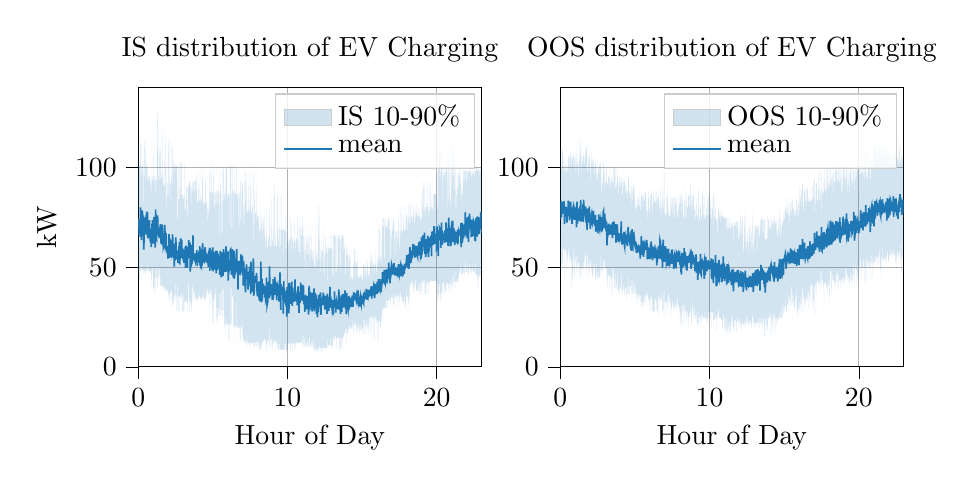
\begin{tikzpicture}

\definecolor{darkgray176}{RGB}{176,176,176}
\definecolor{lightgray204}{RGB}{204,204,204}
\definecolor{steelblue31119180}{RGB}{31,119,180}

\begin{groupplot}[group style={group size=2 by 1}]
\nextgroupplot[
legend cell align={left},
legend style={fill opacity=0.8, draw opacity=1, text opacity=1, draw=lightgray204},
tick align=outside,
tick pos=left,
title={IS distribution of EV Charging},
width=0.49\textwidth,
x grid style={darkgray176},
xlabel={Hour of Day},
xmajorgrids,
xmin=0, xmax=23,
xtick style={color=black},
y grid style={darkgray176},
ylabel={kW},
ymajorgrids,
ymin=0, ymax=139.944507818995,
ytick style={color=black}
]
\path [fill=steelblue31119180, fill opacity=0.2]
(axis cs:0,101.051198652012)
--(axis cs:0,46.4082553290568)
--(axis cs:0.0166666666666667,46.4082553290568)
--(axis cs:0.0333333333333333,50.2973607204393)
--(axis cs:0.05,49.6456751233932)
--(axis cs:0.0666666666666667,43.7805047499783)
--(axis cs:0.0833333333333333,43.7805047499783)
--(axis cs:0.1,48.9274971542461)
--(axis cs:0.116666666666667,48.3433085584562)
--(axis cs:0.133333333333333,48.3433085584562)
--(axis cs:0.15,46.700227615621)
--(axis cs:0.166666666666667,48.9274971542461)
--(axis cs:0.183333333333333,48.3433085584562)
--(axis cs:0.2,48.9274971542461)
--(axis cs:0.216666666666667,48.9274971542461)
--(axis cs:0.233333333333333,50.2973607204393)
--(axis cs:0.25,56.0749377521228)
--(axis cs:0.266666666666667,48.3433085584562)
--(axis cs:0.283333333333333,48.9924069982227)
--(axis cs:0.3,48.9924069982227)
--(axis cs:0.316666666666667,48.3433085584562)
--(axis cs:0.333333333333333,48.1790004641726)
--(axis cs:0.35,48.9924069982227)
--(axis cs:0.366666666666667,46.700227615621)
--(axis cs:0.383333333333333,48.3433085584562)
--(axis cs:0.4,48.1790004641726)
--(axis cs:0.416666666666667,48.3433085584562)
--(axis cs:0.433333333333333,48.3433085584562)
--(axis cs:0.45,48.9274971542461)
--(axis cs:0.466666666666667,46.700227615621)
--(axis cs:0.483333333333333,48.1790004641726)
--(axis cs:0.5,46.700227615621)
--(axis cs:0.516666666666667,48.9274971542461)
--(axis cs:0.533333333333333,50.1668653482176)
--(axis cs:0.55,48.9274971542461)
--(axis cs:0.566666666666667,49.9376474099575)
--(axis cs:0.583333333333333,48.1790004641726)
--(axis cs:0.6,48.9924069982227)
--(axis cs:0.616666666666667,56.0749377521228)
--(axis cs:0.633333333333333,48.1790004641726)
--(axis cs:0.65,48.9924069982227)
--(axis cs:0.666666666666667,48.1790004641726)
--(axis cs:0.683333333333333,48.3433085584562)
--(axis cs:0.7,48.3433085584562)
--(axis cs:0.716666666666667,50.101955504241)
--(axis cs:0.733333333333333,47.3391426929453)
--(axis cs:0.75,48.9274971542461)
--(axis cs:0.766666666666667,47.4101332570924)
--(axis cs:0.783333333333333,47.4101332570924)
--(axis cs:0.8,48.3433085584562)
--(axis cs:0.816666666666667,46.700227615621)
--(axis cs:0.833333333333333,46.700227615621)
--(axis cs:0.85,49.9109917731146)
--(axis cs:0.866666666666667,48.3433085584562)
--(axis cs:0.883333333333333,37.4309630266108)
--(axis cs:0.9,47.2520740052716)
--(axis cs:0.916666666666667,50.0851787969655)
--(axis cs:0.933333333333333,47.2520740052716)
--(axis cs:0.95,50.0851787969655)
--(axis cs:0.966666666666667,49.9109917731146)
--(axis cs:0.983333333333333,50.0851787969655)
--(axis cs:1,39.8984722317046)
--(axis cs:1.01666666666667,36.3243628713829)
--(axis cs:1.03333333333333,39.8984722317046)
--(axis cs:1.05,39.8984722317046)
--(axis cs:1.06666666666667,39.8984722317046)
--(axis cs:1.08333333333333,39.8984722317046)
--(axis cs:1.1,39.5410612956724)
--(axis cs:1.11666666666667,50.2973607204393)
--(axis cs:1.13333333333333,36.3243628713829)
--(axis cs:1.15,36.3243628713829)
--(axis cs:1.16666666666667,53.882459174313)
--(axis cs:1.18333333333333,49.1881123395003)
--(axis cs:1.2,50.0851787969655)
--(axis cs:1.21666666666667,49.1881123395003)
--(axis cs:1.23333333333333,41.1145142223138)
--(axis cs:1.25,50.2761425280919)
--(axis cs:1.26666666666667,40.105974956883)
--(axis cs:1.28333333333333,40.105974956883)
--(axis cs:1.3,49.1881123395003)
--(axis cs:1.31666666666667,41.0136602957708)
--(axis cs:1.33333333333333,40.105974956883)
--(axis cs:1.35,50.2761425280919)
--(axis cs:1.36666666666667,50.0851787969655)
--(axis cs:1.38333333333333,48.8836311747022)
--(axis cs:1.4,48.8836311747022)
--(axis cs:1.41666666666667,48.8836311747022)
--(axis cs:1.43333333333333,41.1145142223138)
--(axis cs:1.45,53.8749303551544)
--(axis cs:1.46666666666667,41.1145142223138)
--(axis cs:1.48333333333333,50.0851787969655)
--(axis cs:1.5,41.0136602957708)
--(axis cs:1.51666666666667,40.3280256521344)
--(axis cs:1.53333333333333,40.3280256521344)
--(axis cs:1.55,41.1145142223138)
--(axis cs:1.56666666666667,40.3058205826093)
--(axis cs:1.58333333333333,41.0136602957708)
--(axis cs:1.6,41.0358653652959)
--(axis cs:1.61666666666667,41.1145142223138)
--(axis cs:1.63333333333333,41.0358653652959)
--(axis cs:1.65,40.3280256521344)
--(axis cs:1.66666666666667,40.105974956883)
--(axis cs:1.68333333333333,37.9553425294954)
--(axis cs:1.7,39.8909117141442)
--(axis cs:1.71666666666667,39.8909117141442)
--(axis cs:1.73333333333333,40.105974956883)
--(axis cs:1.75,40.3058205826093)
--(axis cs:1.76666666666667,40.105974956883)
--(axis cs:1.78333333333333,40.3058205826093)
--(axis cs:1.8,37.9553425294954)
--(axis cs:1.81666666666667,39.8909117141442)
--(axis cs:1.83333333333333,40.3058205826093)
--(axis cs:1.85,37.9553425294954)
--(axis cs:1.86666666666667,40.105974956883)
--(axis cs:1.88333333333333,39.8909117141442)
--(axis cs:1.9,37.9553425294954)
--(axis cs:1.91666666666667,37.9965613741751)
--(axis cs:1.93333333333333,37.9965613741751)
--(axis cs:1.95,37.9553425294954)
--(axis cs:1.96666666666667,37.9553425294954)
--(axis cs:1.98333333333333,37.9553425294954)
--(axis cs:2,43.1878663007301)
--(axis cs:2.01666666666667,33.3337446570414)
--(axis cs:2.03333333333333,38.0011412458062)
--(axis cs:2.05,37.5344015869297)
--(axis cs:2.06666666666667,38.0011412458062)
--(axis cs:2.08333333333333,33.3337446570414)
--(axis cs:2.1,37.5344015869297)
--(axis cs:2.11666666666667,43.7641690846105)
--(axis cs:2.13333333333333,30.3652982073202)
--(axis cs:2.15,38.0011412458062)
--(axis cs:2.16666666666667,38.0011412458062)
--(axis cs:2.18333333333333,43.1878663007301)
--(axis cs:2.2,37.2375569419576)
--(axis cs:2.21666666666667,44.5149577058259)
--(axis cs:2.23333333333333,37.2375569419576)
--(axis cs:2.25,43.1878663007301)
--(axis cs:2.26666666666667,30.3652982073202)
--(axis cs:2.28333333333333,30.3652982073202)
--(axis cs:2.3,30.3652982073202)
--(axis cs:2.31666666666667,41.3536141220537)
--(axis cs:2.33333333333333,31.8792698468649)
--(axis cs:2.35,40.3588389591073)
--(axis cs:2.36666666666667,31.8792698468649)
--(axis cs:2.38333333333333,39.5108820478831)
--(axis cs:2.4,35.5326736882047)
--(axis cs:2.41666666666667,31.8792698468649)
--(axis cs:2.43333333333333,39.4282833355506)
--(axis cs:2.45,35.5326736882047)
--(axis cs:2.46666666666667,35.5326736882047)
--(axis cs:2.48333333333333,35.5326736882047)
--(axis cs:2.5,34.7446440696863)
--(axis cs:2.51666666666667,43.5341666457209)
--(axis cs:2.53333333333333,41.4641446957144)
--(axis cs:2.55,34.7446440696863)
--(axis cs:2.56666666666667,35.5326736882047)
--(axis cs:2.58333333333333,27.6523775030204)
--(axis cs:2.6,35.5326736882047)
--(axis cs:2.61666666666667,41.4676408028323)
--(axis cs:2.63333333333333,41.4676408028323)
--(axis cs:2.65,27.6523775030204)
--(axis cs:2.66666666666667,27.6523775030204)
--(axis cs:2.68333333333333,27.6523775030204)
--(axis cs:2.7,35.5326736882047)
--(axis cs:2.71666666666667,35.5326736882047)
--(axis cs:2.73333333333333,36.9985365134948)
--(axis cs:2.75,27.6523775030204)
--(axis cs:2.76666666666667,36.9985365134948)
--(axis cs:2.78333333333333,35.5326736882047)
--(axis cs:2.8,35.5326736882047)
--(axis cs:2.81666666666667,34.7446440696863)
--(axis cs:2.83333333333333,35.5326736882047)
--(axis cs:2.85,34.7446440696863)
--(axis cs:2.86666666666667,46.9859040125342)
--(axis cs:2.88333333333333,36.9985365134948)
--(axis cs:2.9,36.8519502309658)
--(axis cs:2.91666666666667,35.5326736882047)
--(axis cs:2.93333333333333,34.7446440696863)
--(axis cs:2.95,27.6523775030204)
--(axis cs:2.96666666666667,35.5326736882047)
--(axis cs:2.98333333333333,35.5326736882047)
--(axis cs:3,27.6523775030204)
--(axis cs:3.01666666666667,36.0639206124474)
--(axis cs:3.03333333333333,36.9985365134948)
--(axis cs:3.05,27.6523775030204)
--(axis cs:3.06666666666667,27.6523775030204)
--(axis cs:3.08333333333333,27.6523775030204)
--(axis cs:3.1,41.8511955811132)
--(axis cs:3.11666666666667,32.8591060888288)
--(axis cs:3.13333333333333,32.3384332302479)
--(axis cs:3.15,41.3305227225323)
--(axis cs:3.16666666666667,32.3384332302479)
--(axis cs:3.18333333333333,32.8591060888288)
--(axis cs:3.2,43.7641690846105)
--(axis cs:3.21666666666667,32.8591060888288)
--(axis cs:3.23333333333333,32.8591060888288)
--(axis cs:3.25,32.8591060888288)
--(axis cs:3.26666666666667,32.8591060888288)
--(axis cs:3.28333333333333,32.8591060888288)
--(axis cs:3.3,27.6523775030204)
--(axis cs:3.31666666666667,32.8591060888288)
--(axis cs:3.33333333333333,32.8591060888288)
--(axis cs:3.35,42.7373541088527)
--(axis cs:3.36666666666667,42.8390203831156)
--(axis cs:3.38333333333333,42.6351186314084)
--(axis cs:3.4,32.8591060888288)
--(axis cs:3.41666666666667,32.8591060888288)
--(axis cs:3.43333333333333,27.6523775030204)
--(axis cs:3.45,32.8591060888288)
--(axis cs:3.46666666666667,41.7149993344099)
--(axis cs:3.48333333333333,32.3384332302479)
--(axis cs:3.5,32.8591060888288)
--(axis cs:3.51666666666667,32.8591060888288)
--(axis cs:3.53333333333333,32.8591060888288)
--(axis cs:3.55,27.6523775030204)
--(axis cs:3.56666666666667,41.7149993344099)
--(axis cs:3.58333333333333,27.6523775030204)
--(axis cs:3.6,40.8294100098518)
--(axis cs:3.61666666666667,40.8294100098518)
--(axis cs:3.63333333333333,41.7149993344099)
--(axis cs:3.65,32.8591060888288)
--(axis cs:3.66666666666667,41.4087371512709)
--(axis cs:3.68333333333333,38.6523775030204)
--(axis cs:3.7,32.8591060888288)
--(axis cs:3.71666666666667,38.0730503616012)
--(axis cs:3.73333333333333,41.4087371512709)
--(axis cs:3.75,38.6523775030204)
--(axis cs:3.76666666666667,32.8591060888288)
--(axis cs:3.78333333333333,38.6523775030204)
--(axis cs:3.8,39.3531040122312)
--(axis cs:3.81666666666667,34.5422688759187)
--(axis cs:3.83333333333333,34.5422688759187)
--(axis cs:3.85,34.5422688759187)
--(axis cs:3.86666666666667,39.3531040122312)
--(axis cs:3.88333333333333,32.8292291268943)
--(axis cs:3.9,32.8292291268943)
--(axis cs:3.91666666666667,34.5422688759187)
--(axis cs:3.93333333333333,34.3739525972097)
--(axis cs:3.95,32.8292291268943)
--(axis cs:3.96666666666667,34.3739525972097)
--(axis cs:3.98333333333333,34.3739525972097)
--(axis cs:4,34.3739525972097)
--(axis cs:4.01666666666667,36.9327243532557)
--(axis cs:4.03333333333333,34.5422688759187)
--(axis cs:4.05,34.3739525972097)
--(axis cs:4.06666666666667,34.5422688759187)
--(axis cs:4.08333333333333,37.1288071742804)
--(axis cs:4.1,36.5030970861655)
--(axis cs:4.11666666666667,36.1386979864318)
--(axis cs:4.13333333333333,34.5422688759187)
--(axis cs:4.15,36.3070142651408)
--(axis cs:4.16666666666667,34.3739525972097)
--(axis cs:4.18333333333333,34.5422688759187)
--(axis cs:4.2,32.8591060888288)
--(axis cs:4.21666666666667,32.8591060888288)
--(axis cs:4.23333333333333,34.3739525972097)
--(axis cs:4.25,34.5422688759187)
--(axis cs:4.26666666666667,34.3739525972097)
--(axis cs:4.28333333333333,36.3070142651408)
--(axis cs:4.3,36.3070142651408)
--(axis cs:4.31666666666667,34.5422688759187)
--(axis cs:4.33333333333333,34.5422688759187)
--(axis cs:4.35,34.3739525972097)
--(axis cs:4.36666666666667,36.3070142651408)
--(axis cs:4.38333333333333,41.8308118454434)
--(axis cs:4.4,32.8591060888288)
--(axis cs:4.41666666666667,34.5422688759187)
--(axis cs:4.43333333333333,36.5030970861655)
--(axis cs:4.45,32.8591060888288)
--(axis cs:4.46666666666667,34.3739525972097)
--(axis cs:4.48333333333333,34.5422688759187)
--(axis cs:4.5,34.5422688759187)
--(axis cs:4.51666666666667,33.8275158197547)
--(axis cs:4.53333333333333,34.5422688759187)
--(axis cs:4.55,34.5422688759187)
--(axis cs:4.56666666666667,42.0268946664681)
--(axis cs:4.58333333333333,39.1246439108624)
--(axis cs:4.6,35.5922612089768)
--(axis cs:4.61666666666667,36.5030970861655)
--(axis cs:4.63333333333333,41.5173046621047)
--(axis cs:4.65,39.4159268913843)
--(axis cs:4.66666666666667,39.1246439108624)
--(axis cs:4.68333333333333,36.5030970861655)
--(axis cs:4.7,36.5030970861655)
--(axis cs:4.71666666666667,36.5030970861655)
--(axis cs:4.73333333333333,36.5030970861655)
--(axis cs:4.75,39.4159268913843)
--(axis cs:4.76666666666667,39.4159268913843)
--(axis cs:4.78333333333333,39.4159268913843)
--(axis cs:4.8,22.024516215805)
--(axis cs:4.81666666666667,36.5030970861655)
--(axis cs:4.83333333333333,41.7507910810737)
--(axis cs:4.85,36.5030970861655)
--(axis cs:4.86666666666667,39.1246439108624)
--(axis cs:4.88333333333333,36.5030970861655)
--(axis cs:4.9,36.5030970861655)
--(axis cs:4.91666666666667,39.1246439108624)
--(axis cs:4.93333333333333,37.6767858238263)
--(axis cs:4.95,22.024516215805)
--(axis cs:4.96666666666667,22.024516215805)
--(axis cs:4.98333333333333,41.0006095129766)
--(axis cs:5,41.7507910810737)
--(axis cs:5.01666666666667,22.024516215805)
--(axis cs:5.03333333333333,34.2489754001031)
--(axis cs:5.05,22.024516215805)
--(axis cs:5.06666666666667,41.0006095129766)
--(axis cs:5.08333333333333,34.2489754001031)
--(axis cs:5.1,34.2489754001031)
--(axis cs:5.11666666666667,42.3852050560905)
--(axis cs:5.13333333333333,33.0265294816733)
--(axis cs:5.15,39.7781635945468)
--(axis cs:5.16666666666667,41.0006095129766)
--(axis cs:5.18333333333333,41.7507910810737)
--(axis cs:5.2,34.2489754001031)
--(axis cs:5.21666666666667,40.1494053294386)
--(axis cs:5.23333333333333,25.3656918298315)
--(axis cs:5.25,22.024516215805)
--(axis cs:5.26666666666667,25.7369335647234)
--(axis cs:5.28333333333333,40.1494053294386)
--(axis cs:5.3,25.3656918298315)
--(axis cs:5.31666666666667,25.3656918298315)
--(axis cs:5.33333333333333,22.024516215805)
--(axis cs:5.35,40.1494053294386)
--(axis cs:5.36666666666667,25.3656918298315)
--(axis cs:5.38333333333333,25.7369335647234)
--(axis cs:5.4,39.7781635945468)
--(axis cs:5.41666666666667,25.7369335647234)
--(axis cs:5.43333333333333,40.1494053294386)
--(axis cs:5.45,40.1494053294386)
--(axis cs:5.46666666666667,22.024516215805)
--(axis cs:5.48333333333333,40.1494053294386)
--(axis cs:5.5,25.7369335647234)
--(axis cs:5.51666666666667,25.7369335647234)
--(axis cs:5.53333333333333,40.1494053294386)
--(axis cs:5.55,40.1494053294386)
--(axis cs:5.56666666666667,25.7369335647234)
--(axis cs:5.58333333333333,41.7507910810737)
--(axis cs:5.6,40.1494053294386)
--(axis cs:5.61666666666667,25.7369335647234)
--(axis cs:5.63333333333333,25.3656918298315)
--(axis cs:5.65,41.7507910810737)
--(axis cs:5.66666666666667,41.7507910810737)
--(axis cs:5.68333333333333,22.024516215805)
--(axis cs:5.7,41.7507910810737)
--(axis cs:5.71666666666667,40.1494053294386)
--(axis cs:5.73333333333333,42.3217636585888)
--(axis cs:5.75,25.3656918298315)
--(axis cs:5.76666666666667,40.1494053294386)
--(axis cs:5.78333333333333,16.9523046469496)
--(axis cs:5.8,39.7781635945468)
--(axis cs:5.81666666666667,16.9523046469496)
--(axis cs:5.83333333333333,22.024516215805)
--(axis cs:5.85,39.7781635945468)
--(axis cs:5.86666666666667,19.1535744277441)
--(axis cs:5.88333333333333,39.7781635945468)
--(axis cs:5.9,22.024516215805)
--(axis cs:5.91666666666667,39.7781635945468)
--(axis cs:5.93333333333333,19.1535744277441)
--(axis cs:5.95,22.024516215805)
--(axis cs:5.96666666666667,21.0312119365733)
--(axis cs:5.98333333333333,21.0312119365733)
--(axis cs:6,22.024516215805)
--(axis cs:6.01666666666667,21.0312119365733)
--(axis cs:6.03333333333333,12.0914734234885)
--(axis cs:6.05,22.024516215805)
--(axis cs:6.06666666666667,22.024516215805)
--(axis cs:6.08333333333333,21.0312119365733)
--(axis cs:6.1,22.024516215805)
--(axis cs:6.11666666666667,39.7781635945468)
--(axis cs:6.13333333333333,12.0914734234885)
--(axis cs:6.15,21.0312119365733)
--(axis cs:6.16666666666667,21.0312119365733)
--(axis cs:6.18333333333333,22.024516215805)
--(axis cs:6.2,41.7507910810737)
--(axis cs:6.21666666666667,39.7781635945468)
--(axis cs:6.23333333333333,38.7848593153152)
--(axis cs:6.25,22.024516215805)
--(axis cs:6.26666666666667,21.0312119365733)
--(axis cs:6.28333333333333,35.3707974737127)
--(axis cs:6.3,41.2610837343143)
--(axis cs:6.31666666666667,35.3707974737127)
--(axis cs:6.33333333333333,36.8537176134802)
--(axis cs:6.35,35.3707974737127)
--(axis cs:6.36666666666667,21.0312119365733)
--(axis cs:6.38333333333333,35.3707974737127)
--(axis cs:6.4,34.377493194481)
--(axis cs:6.41666666666667,19.6067688413599)
--(axis cs:6.43333333333333,41.7507910810737)
--(axis cs:6.45,19.6067688413599)
--(axis cs:6.46666666666667,36.8537176134802)
--(axis cs:6.48333333333333,12.0914734234885)
--(axis cs:6.5,19.6067688413599)
--(axis cs:6.51666666666667,20.4418016655678)
--(axis cs:6.53333333333333,20.4418016655678)
--(axis cs:6.55,20.4418016655678)
--(axis cs:6.56666666666667,19.6067688413599)
--(axis cs:6.58333333333333,31.9318007532983)
--(axis cs:6.6,36.361525927462)
--(axis cs:6.61666666666667,20.4418016655678)
--(axis cs:6.63333333333333,19.6067688413599)
--(axis cs:6.65,20.4234175523232)
--(axis cs:6.66666666666667,20.4418016655678)
--(axis cs:6.68333333333333,12.0914734234885)
--(axis cs:6.7,30.3513412322678)
--(axis cs:6.71666666666667,20.4418016655678)
--(axis cs:6.73333333333333,20.2579605331211)
--(axis cs:6.75,20.4418016655678)
--(axis cs:6.76666666666667,19.4413118221578)
--(axis cs:6.78333333333333,19.6067688413599)
--(axis cs:6.8,20.4234175523232)
--(axis cs:6.81666666666667,12.0914734234885)
--(axis cs:6.83333333333333,20.2579605331211)
--(axis cs:6.85,12.0914734234885)
--(axis cs:6.86666666666667,20.2579605331211)
--(axis cs:6.88333333333333,20.4234175523232)
--(axis cs:6.9,20.4234175523232)
--(axis cs:6.91666666666667,20.4234175523232)
--(axis cs:6.93333333333333,20.2579605331211)
--(axis cs:6.95,14.2913260246953)
--(axis cs:6.96666666666667,22.4995486749024)
--(axis cs:6.98333333333333,22.7486140239892)
--(axis cs:7,19.4413118221578)
--(axis cs:7.01666666666667,14.2913260246953)
--(axis cs:7.03333333333333,12.648510057156)
--(axis cs:7.05,12.0914734234885)
--(axis cs:7.06666666666667,12.648510057156)
--(axis cs:7.08333333333333,19.4130768481344)
--(axis cs:7.1,14.1270444279414)
--(axis cs:7.11666666666667,12.648510057156)
--(axis cs:7.13333333333333,14.0713407645746)
--(axis cs:7.15,12.0914734234885)
--(axis cs:7.16666666666667,12.0914734234885)
--(axis cs:7.18333333333333,12.0914734234885)
--(axis cs:7.2,11.7772828342865)
--(axis cs:7.21666666666667,18.7366201690366)
--(axis cs:7.23333333333333,18.6809165056698)
--(axis cs:7.25,8.94956753146855)
--(axis cs:7.26666666666667,12.0914734234885)
--(axis cs:7.28333333333333,12.0914734234885)
--(axis cs:7.3,18.7366201690366)
--(axis cs:7.31666666666667,12.648510057156)
--(axis cs:7.33333333333333,11.7772828342865)
--(axis cs:7.35,11.7772828342865)
--(axis cs:7.36666666666667,11.7772828342865)
--(axis cs:7.38333333333333,12.0914734234885)
--(axis cs:7.4,12.5928063937893)
--(axis cs:7.41666666666667,11.7772828342865)
--(axis cs:7.43333333333333,12.0914734234885)
--(axis cs:7.45,11.7772828342865)
--(axis cs:7.46666666666667,8.94956753146855)
--(axis cs:7.48333333333333,12.5928063937893)
--(axis cs:7.5,12.5928063937893)
--(axis cs:7.51666666666667,12.2786158045873)
--(axis cs:7.53333333333333,11.7772828342865)
--(axis cs:7.55,12.0914734234885)
--(axis cs:7.56666666666667,11.7772828342865)
--(axis cs:7.58333333333333,11.7772828342865)
--(axis cs:7.6,12.648510057156)
--(axis cs:7.61666666666667,12.0914734234885)
--(axis cs:7.63333333333333,11.7772828342865)
--(axis cs:7.65,11.7772828342865)
--(axis cs:7.66666666666667,12.648510057156)
--(axis cs:7.68333333333333,11.7772828342865)
--(axis cs:7.7,12.0914734234885)
--(axis cs:7.71666666666667,12.2786158045873)
--(axis cs:7.73333333333333,8.94956753146855)
--(axis cs:7.75,12.5928063937893)
--(axis cs:7.76666666666667,12.5928063937893)
--(axis cs:7.78333333333333,12.0914734234885)
--(axis cs:7.8,8.78967793533981)
--(axis cs:7.81666666666667,12.5928063937893)
--(axis cs:7.83333333333333,12.0914734234885)
--(axis cs:7.85,12.648510057156)
--(axis cs:7.86666666666667,12.0914734234885)
--(axis cs:7.88333333333333,8.78967793533981)
--(axis cs:7.9,12.0914734234885)
--(axis cs:7.91666666666667,13.5307287844962)
--(axis cs:7.93333333333333,12.648510057156)
--(axis cs:7.95,12.648510057156)
--(axis cs:7.96666666666667,8.78967793533981)
--(axis cs:7.98333333333333,8.78967793533981)
--(axis cs:8,12.0914734234885)
--(axis cs:8.01666666666667,12.0914734234885)
--(axis cs:8.03333333333333,12.648510057156)
--(axis cs:8.05,12.648510057156)
--(axis cs:8.06666666666667,12.2626268449744)
--(axis cs:8.08333333333333,12.648510057156)
--(axis cs:8.1,8.78967793533981)
--(axis cs:8.11666666666667,12.648510057156)
--(axis cs:8.13333333333333,8.78967793533981)
--(axis cs:8.15,8.78967793533981)
--(axis cs:8.16666666666667,8.78967793533981)
--(axis cs:8.18333333333333,8.38358016700609)
--(axis cs:8.2,8.77405536742398)
--(axis cs:8.21666666666667,13.5307287844962)
--(axis cs:8.23333333333333,8.78967793533981)
--(axis cs:8.25,13.5307287844962)
--(axis cs:8.26666666666667,8.63345225618151)
--(axis cs:8.28333333333333,13.4280320955276)
--(axis cs:8.3,12.50376189481)
--(axis cs:8.31666666666667,12.50376189481)
--(axis cs:8.33333333333333,12.50376189481)
--(axis cs:8.35,12.1167309309472)
--(axis cs:8.36666666666667,12.50376189481)
--(axis cs:8.38333333333333,13.0410011316647)
--(axis cs:8.4,13.0410011316647)
--(axis cs:8.41666666666667,13.5307287844962)
--(axis cs:8.43333333333333,16.1770195747946)
--(axis cs:8.45,13.5307287844962)
--(axis cs:8.46666666666667,13.5307287844962)
--(axis cs:8.48333333333333,13.5307287844962)
--(axis cs:8.5,13.5307287844962)
--(axis cs:8.51666666666667,13.5307287844962)
--(axis cs:8.53333333333333,16.1770195747946)
--(axis cs:8.55,8.63345225618151)
--(axis cs:8.56666666666667,8.63345225618151)
--(axis cs:8.58333333333333,15.9123904957648)
--(axis cs:8.6,8.63345225618151)
--(axis cs:8.61666666666667,13.0410011316647)
--(axis cs:8.63333333333333,13.5307287844962)
--(axis cs:8.65,13.0410011316647)
--(axis cs:8.66666666666667,15.9123904957648)
--(axis cs:8.68333333333333,13.5307287844962)
--(axis cs:8.7,8.63345225618151)
--(axis cs:8.71666666666667,13.0410011316647)
--(axis cs:8.73333333333333,13.0410011316647)
--(axis cs:8.75,15.9123904957648)
--(axis cs:8.76666666666667,15.9123904957648)
--(axis cs:8.78333333333333,8.63345225618151)
--(axis cs:8.8,33.148866820808)
--(axis cs:8.81666666666667,15.9123904957648)
--(axis cs:8.83333333333333,8.63345225618151)
--(axis cs:8.85,15.9123904957648)
--(axis cs:8.86666666666667,13.0410011316647)
--(axis cs:8.88333333333333,13.5307287844962)
--(axis cs:8.9,13.5307287844962)
--(axis cs:8.91666666666667,16.6986382485617)
--(axis cs:8.93333333333333,8.63345225618151)
--(axis cs:8.95,16.7565958789802)
--(axis cs:8.96666666666667,16.1770195747946)
--(axis cs:8.98333333333333,8.63345225618151)
--(axis cs:9,13.8035105586078)
--(axis cs:9.01666666666667,16.7565958789802)
--(axis cs:9.03333333333333,8.63345225618151)
--(axis cs:9.05,13.8035105586078)
--(axis cs:9.06666666666667,11.7033007394819)
--(axis cs:9.08333333333333,13.6275990042874)
--(axis cs:9.1,16.7565958789802)
--(axis cs:9.11666666666667,12.0443950154042)
--(axis cs:9.13333333333333,13.8035105586078)
--(axis cs:9.15,13.6275990042874)
--(axis cs:9.16666666666667,18.1362018914549)
--(axis cs:9.18333333333333,12.0443950154042)
--(axis cs:9.2,13.6275990042874)
--(axis cs:9.21666666666667,8.63345225618151)
--(axis cs:9.23333333333333,13.8035105586078)
--(axis cs:9.25,16.7565958789802)
--(axis cs:9.26666666666667,11.7033007394819)
--(axis cs:9.28333333333333,13.2865047283652)
--(axis cs:9.3,12.0443950154042)
--(axis cs:9.31666666666667,8.63345225618151)
--(axis cs:9.33333333333333,12.0443950154042)
--(axis cs:9.35,11.7033007394819)
--(axis cs:9.36666666666667,11.7033007394819)
--(axis cs:9.38333333333333,8.63345225618151)
--(axis cs:9.4,12.0443950154042)
--(axis cs:9.41666666666667,8.63345225618151)
--(axis cs:9.43333333333333,11.8829378635147)
--(axis cs:9.45,11.5579893027814)
--(axis cs:9.46666666666667,11.5344971646062)
--(axis cs:9.48333333333333,8.63345225618151)
--(axis cs:9.5,11.8829378635147)
--(axis cs:9.51666666666667,8.60996011800633)
--(axis cs:9.53333333333333,8.60996011800633)
--(axis cs:9.55,8.39853087442975)
--(axis cs:9.56666666666667,8.63345225618151)
--(axis cs:9.58333333333333,8.60996011800633)
--(axis cs:9.6,12.0282493002152)
--(axis cs:9.61666666666667,8.63345225618151)
--(axis cs:9.63333333333333,8.63345225618151)
--(axis cs:9.65,11.8829378635147)
--(axis cs:9.66666666666667,8.60996011800633)
--(axis cs:9.68333333333333,8.63345225618151)
--(axis cs:9.7,11.5579893027814)
--(axis cs:9.71666666666667,8.60996011800633)
--(axis cs:9.73333333333333,8.63345225618151)
--(axis cs:9.75,11.8829378635147)
--(axis cs:9.76666666666667,8.63345225618151)
--(axis cs:9.78333333333333,12.0282493002152)
--(axis cs:9.8,11.5579893027814)
--(axis cs:9.81666666666667,8.60996011800633)
--(axis cs:9.83333333333333,8.39853087442975)
--(axis cs:9.85,11.8829378635147)
--(axis cs:9.86666666666667,11.5344971646062)
--(axis cs:9.88333333333333,11.5579893027814)
--(axis cs:9.9,8.39853087442975)
--(axis cs:9.91666666666667,8.39853087442975)
--(axis cs:9.93333333333333,8.63345225618151)
--(axis cs:9.95,8.39853087442975)
--(axis cs:9.96666666666667,8.63345225618151)
--(axis cs:9.98333333333333,11.5579893027814)
--(axis cs:10,8.39853087442975)
--(axis cs:10.0166666666667,11.8829378635147)
--(axis cs:10.0333333333333,12.0282493002152)
--(axis cs:10.05,12.0282493002152)
--(axis cs:10.0666666666667,11.5344971646062)
--(axis cs:10.0833333333333,11.5344971646062)
--(axis cs:10.1,11.8829378635147)
--(axis cs:10.1166666666667,11.8829378635147)
--(axis cs:10.1333333333333,12.711487294508)
--(axis cs:10.15,12.7856086588529)
--(axis cs:10.1666666666667,11.8829378635147)
--(axis cs:10.1833333333333,8.39853087442975)
--(axis cs:10.2,11.5344971646062)
--(axis cs:10.2166666666667,12.0282493002152)
--(axis cs:10.2333333333333,8.39853087442975)
--(axis cs:10.25,11.5344971646062)
--(axis cs:10.2666666666667,12.0282493002152)
--(axis cs:10.2833333333333,12.0282493002152)
--(axis cs:10.3,11.8829378635147)
--(axis cs:10.3166666666667,8.39853087442975)
--(axis cs:10.3333333333333,11.8829378635147)
--(axis cs:10.35,11.8829378635147)
--(axis cs:10.3666666666667,11.5344971646062)
--(axis cs:10.3833333333333,11.8829378635147)
--(axis cs:10.4,11.8829378635147)
--(axis cs:10.4166666666667,12.0282493002152)
--(axis cs:10.4333333333333,11.5344971646062)
--(axis cs:10.45,12.0282493002152)
--(axis cs:10.4666666666667,8.39853087442975)
--(axis cs:10.4833333333333,8.39853087442975)
--(axis cs:10.5,21.9715974539194)
--(axis cs:10.5166666666667,8.39853087442975)
--(axis cs:10.5333333333333,11.8829378635147)
--(axis cs:10.55,12.0282493002152)
--(axis cs:10.5666666666667,12.0443950154042)
--(axis cs:10.5833333333333,11.5344971646062)
--(axis cs:10.6,12.0282493002152)
--(axis cs:10.6166666666667,13.3619146722039)
--(axis cs:10.6333333333333,13.5083057451817)
--(axis cs:10.65,12.0282493002152)
--(axis cs:10.6666666666667,11.8829378635147)
--(axis cs:10.6833333333333,12.0282493002152)
--(axis cs:10.7,12.0443950154042)
--(axis cs:10.7166666666667,12.0443950154042)
--(axis cs:10.7333333333333,12.0282493002152)
--(axis cs:10.75,11.8829378635147)
--(axis cs:10.7666666666667,11.8829378635147)
--(axis cs:10.7833333333333,12.0282493002152)
--(axis cs:10.8,11.8829378635147)
--(axis cs:10.8166666666667,12.0443950154042)
--(axis cs:10.8333333333333,11.7560138384262)
--(axis cs:10.85,13.5083057451817)
--(axis cs:10.8666666666667,12.0443950154042)
--(axis cs:10.8833333333333,13.3619146722039)
--(axis cs:10.9,12.0443950154042)
--(axis cs:10.9166666666667,11.7560138384262)
--(axis cs:10.9333333333333,13.5083057451817)
--(axis cs:10.95,13.5083057451817)
--(axis cs:10.9666666666667,11.7560138384262)
--(axis cs:10.9833333333333,11.7560138384262)
--(axis cs:11,12.0443950154042)
--(axis cs:11.0166666666667,9.16058324562402)
--(axis cs:11.0333333333333,21.0740355893363)
--(axis cs:11.05,9.16058324562402)
--(axis cs:11.0666666666667,13.3619146722039)
--(axis cs:11.0833333333333,18.8464673714007)
--(axis cs:11.1,11.7945928418351)
--(axis cs:11.1166666666667,18.8464673714007)
--(axis cs:11.1333333333333,13.5083057451817)
--(axis cs:11.15,13.3619146722039)
--(axis cs:11.1666666666667,9.54637327971365)
--(axis cs:11.1833333333333,10.9516232166614)
--(axis cs:11.2,13.5083057451817)
--(axis cs:11.2166666666667,9.54637327971365)
--(axis cs:11.2333333333333,10.8110982229666)
--(axis cs:11.25,9.54637327971365)
--(axis cs:11.2666666666667,10.9516232166614)
--(axis cs:11.2833333333333,10.9516232166614)
--(axis cs:11.3,10.9516232166614)
--(axis cs:11.3166666666667,10.9516232166614)
--(axis cs:11.3333333333333,13.2526374923296)
--(axis cs:11.35,13.5083057451817)
--(axis cs:11.3666666666667,13.5083057451817)
--(axis cs:11.3833333333333,10.9516232166614)
--(axis cs:11.4,10.9516232166614)
--(axis cs:11.4166666666667,9.54637327971365)
--(axis cs:11.4333333333333,9.54637327971365)
--(axis cs:11.45,18.9928584443784)
--(axis cs:11.4666666666667,18.9928584443784)
--(axis cs:11.4833333333333,10.8110982229666)
--(axis cs:11.5,10.8110982229666)
--(axis cs:11.5166666666667,10.8110982229666)
--(axis cs:11.5333333333333,9.54637327971365)
--(axis cs:11.55,10.8110982229666)
--(axis cs:11.5666666666667,13.2526374923296)
--(axis cs:11.5833333333333,9.54637327971365)
--(axis cs:11.6,10.9516232166614)
--(axis cs:11.6166666666667,13.2526374923296)
--(axis cs:11.6333333333333,13.2526374923296)
--(axis cs:11.65,9.54637327971365)
--(axis cs:11.6666666666667,13.5083057451817)
--(axis cs:11.6833333333333,10.8110982229666)
--(axis cs:11.7,18.7371901915264)
--(axis cs:11.7166666666667,9.3405979284176)
--(axis cs:11.7333333333333,18.9928584443784)
--(axis cs:11.75,9.3405979284176)
--(axis cs:11.7666666666667,9.54637327971365)
--(axis cs:11.7833333333333,13.5083057451817)
--(axis cs:11.8,9.54637327971365)
--(axis cs:11.8166666666667,7.48861976675316)
--(axis cs:11.8333333333333,9.3405979284176)
--(axis cs:11.85,9.3405979284176)
--(axis cs:11.8666666666667,9.54637327971365)
--(axis cs:11.8833333333333,7.48861976675316)
--(axis cs:11.9,7.48861976675316)
--(axis cs:11.9166666666667,13.1121124986349)
--(axis cs:11.9333333333333,7.48861976675316)
--(axis cs:11.95,9.54637327971365)
--(axis cs:11.9666666666667,9.54637327971365)
--(axis cs:11.9833333333333,9.54637327971365)
--(axis cs:12,7.48861976675316)
--(axis cs:12.0166666666667,9.54637327971365)
--(axis cs:12.0333333333333,9.54637327971365)
--(axis cs:12.05,7.48861976675316)
--(axis cs:12.0666666666667,7.48861976675316)
--(axis cs:12.0833333333333,9.54637327971365)
--(axis cs:12.1,9.54637327971365)
--(axis cs:12.1166666666667,15.4317821113449)
--(axis cs:12.1333333333333,9.3405979284176)
--(axis cs:12.15,11.013307233812)
--(axis cs:12.1666666666667,9.3405979284176)
--(axis cs:12.1833333333333,10.8666138384022)
--(axis cs:12.2,9.54637327971365)
--(axis cs:12.2166666666667,11.013307233812)
--(axis cs:12.2333333333333,7.48861976675316)
--(axis cs:12.25,7.48861976675316)
--(axis cs:12.2666666666667,10.8666138384022)
--(axis cs:12.2833333333333,7.48861976675316)
--(axis cs:12.3,9.54637327971365)
--(axis cs:12.3166666666667,9.54637327971365)
--(axis cs:12.3333333333333,9.3405979284176)
--(axis cs:12.35,9.54637327971365)
--(axis cs:12.3666666666667,9.3405979284176)
--(axis cs:12.3833333333333,10.8666138384022)
--(axis cs:12.4,9.3405979284176)
--(axis cs:12.4166666666667,7.48861976675316)
--(axis cs:12.4333333333333,11.013307233812)
--(axis cs:12.45,10.8666138384022)
--(axis cs:12.4666666666667,9.3405979284176)
--(axis cs:12.4833333333333,9.3405979284176)
--(axis cs:12.5,9.54637327971365)
--(axis cs:12.5166666666667,9.54637327971365)
--(axis cs:12.5333333333333,9.54637327971365)
--(axis cs:12.55,9.3405979284176)
--(axis cs:12.5666666666667,9.54637327971365)
--(axis cs:12.5833333333333,7.48861976675316)
--(axis cs:12.6,11.013307233812)
--(axis cs:12.6166666666667,9.54637327971365)
--(axis cs:12.6333333333333,9.3405979284176)
--(axis cs:12.65,9.3405979284176)
--(axis cs:12.6666666666667,9.54637327971365)
--(axis cs:12.6833333333333,14.1979978732472)
--(axis cs:12.7,14.55185238874)
--(axis cs:12.7166666666667,10.8666138384022)
--(axis cs:12.7333333333333,11.013307233812)
--(axis cs:12.75,19.7354451506645)
--(axis cs:12.7666666666667,9.54637327971365)
--(axis cs:12.7833333333333,10.8666138384022)
--(axis cs:12.8,10.8666138384022)
--(axis cs:12.8166666666667,11.013307233812)
--(axis cs:12.8333333333333,10.8666138384022)
--(axis cs:12.85,10.8666138384022)
--(axis cs:12.8666666666667,11.013307233812)
--(axis cs:12.8833333333333,10.8666138384022)
--(axis cs:12.9,14.1979978732472)
--(axis cs:12.9166666666667,14.1979978732472)
--(axis cs:12.9333333333333,14.1979978732472)
--(axis cs:12.95,9.54637327971365)
--(axis cs:12.9666666666667,10.8666138384022)
--(axis cs:12.9833333333333,11.013307233812)
--(axis cs:13,13.0546039219083)
--(axis cs:13.0166666666667,9.54637327971365)
--(axis cs:13.0333333333333,9.54637327971365)
--(axis cs:13.05,14.4021275420568)
--(axis cs:13.0666666666667,13.0546039219083)
--(axis cs:13.0833333333333,14.55185238874)
--(axis cs:13.1,15.6651224554917)
--(axis cs:13.1166666666667,15.5537954488165)
--(axis cs:13.1333333333333,14.55185238874)
--(axis cs:13.15,15.5537954488165)
--(axis cs:13.1666666666667,13.0546039219083)
--(axis cs:13.1833333333333,15.5537954488165)
--(axis cs:13.2,15.5537954488165)
--(axis cs:13.2166666666667,15.5537954488165)
--(axis cs:13.2333333333333,14.4021275420568)
--(axis cs:13.25,14.55185238874)
--(axis cs:13.2666666666667,14.55185238874)
--(axis cs:13.2833333333333,8.32399101069401)
--(axis cs:13.3,14.55185238874)
--(axis cs:13.3166666666667,14.55185238874)
--(axis cs:13.3333333333333,14.55185238874)
--(axis cs:13.35,14.55185238874)
--(axis cs:13.3666666666667,19.7354451506645)
--(axis cs:13.3833333333333,13.9290662509354)
--(axis cs:13.4,14.55185238874)
--(axis cs:13.4166666666667,15.6651224554917)
--(axis cs:13.4333333333333,14.55185238874)
--(axis cs:13.45,15.6651224554917)
--(axis cs:13.4666666666667,8.32399101069401)
--(axis cs:13.4833333333333,14.55185238874)
--(axis cs:13.5,15.6651224554917)
--(axis cs:13.5166666666667,8.32399101069401)
--(axis cs:13.5333333333333,16.0980528865696)
--(axis cs:13.55,16.0980528865696)
--(axis cs:13.5666666666667,8.32399101069401)
--(axis cs:13.5833333333333,16.0980528865696)
--(axis cs:13.6,14.55185238874)
--(axis cs:13.6166666666667,14.55185238874)
--(axis cs:13.6333333333333,8.32399101069401)
--(axis cs:13.65,13.9290662509354)
--(axis cs:13.6666666666667,8.32399101069401)
--(axis cs:13.6833333333333,16.269852941884)
--(axis cs:13.7,14.55185238874)
--(axis cs:13.7166666666667,13.9290662509354)
--(axis cs:13.7333333333333,19.1126590128599)
--(axis cs:13.75,14.55185238874)
--(axis cs:13.7666666666667,16.0980528865696)
--(axis cs:13.7833333333333,16.269852941884)
--(axis cs:13.8,16.269852941884)
--(axis cs:13.8166666666667,20.3113999019894)
--(axis cs:13.8333333333333,15.475266748765)
--(axis cs:13.85,19.9072452059789)
--(axis cs:13.8666666666667,19.9072452059789)
--(axis cs:13.8833333333333,16.269852941884)
--(axis cs:13.9,19.9072452059789)
--(axis cs:13.9166666666667,20.3113999019894)
--(axis cs:13.9333333333333,8.32399101069401)
--(axis cs:13.95,20.7207464226094)
--(axis cs:13.9666666666667,19.9072452059789)
--(axis cs:13.9833333333333,19.9072452059789)
--(axis cs:14,16.269852941884)
--(axis cs:14.0166666666667,19.323991010694)
--(axis cs:14.0333333333333,16.269852941884)
--(axis cs:14.05,19.018577203813)
--(axis cs:14.0666666666667,19.018577203813)
--(axis cs:14.0833333333333,20.2126590128599)
--(axis cs:14.1,16.269852941884)
--(axis cs:14.1166666666667,19.323991010694)
--(axis cs:14.1333333333333,20.7207464226094)
--(axis cs:14.15,19.323991010694)
--(axis cs:14.1666666666667,24.7853020290367)
--(axis cs:14.1833333333333,21.21529014269)
--(axis cs:14.2,19.323991010694)
--(axis cs:14.2166666666667,19.018577203813)
--(axis cs:14.2333333333333,19.323991010694)
--(axis cs:14.25,21.21529014269)
--(axis cs:14.2666666666667,19.323991010694)
--(axis cs:14.2833333333333,21.0261602294904)
--(axis cs:14.3,19.323991010694)
--(axis cs:14.3166666666667,19.018577203813)
--(axis cs:14.3333333333333,21.0261602294904)
--(axis cs:14.35,24.428300840402)
--(axis cs:14.3666666666667,21.21529014269)
--(axis cs:14.3833333333333,19.323991010694)
--(axis cs:14.4,16.269852941884)
--(axis cs:14.4166666666667,16.269852941884)
--(axis cs:14.4333333333333,20.7207464226094)
--(axis cs:14.45,21.21529014269)
--(axis cs:14.4666666666667,25.1412616744757)
--(axis cs:14.4833333333333,21.21529014269)
--(axis cs:14.5,21.21529014269)
--(axis cs:14.5166666666667,24.6512254193876)
--(axis cs:14.5333333333333,21.21529014269)
--(axis cs:14.55,21.21529014269)
--(axis cs:14.5666666666667,23.4445359325451)
--(axis cs:14.5833333333333,16.269852941884)
--(axis cs:14.6,16.269852941884)
--(axis cs:14.6166666666667,23.4445359325451)
--(axis cs:14.6333333333333,23.4445359325451)
--(axis cs:14.65,18.6888883890972)
--(axis cs:14.6666666666667,16.269852941884)
--(axis cs:14.6833333333333,18.9576701054542)
--(axis cs:14.7,18.9576701054542)
--(axis cs:14.7166666666667,23.0648493846628)
--(axis cs:14.7333333333333,23.5212026379082)
--(axis cs:14.75,18.6888883890972)
--(axis cs:14.7666666666667,18.9576701054542)
--(axis cs:14.7833333333333,18.6888883890972)
--(axis cs:14.8,16.269852941884)
--(axis cs:14.8166666666667,16.269852941884)
--(axis cs:14.8333333333333,24.6588920899239)
--(axis cs:14.85,18.6888883890972)
--(axis cs:14.8666666666667,18.6888883890972)
--(axis cs:14.8833333333333,24.6588920899239)
--(axis cs:14.9,18.9576701054542)
--(axis cs:14.9166666666667,18.6888883890972)
--(axis cs:14.9333333333333,18.9576701054542)
--(axis cs:14.95,18.9576701054542)
--(axis cs:14.9666666666667,23.0648493846628)
--(axis cs:14.9833333333333,18.6888883890972)
--(axis cs:15,16.269852941884)
--(axis cs:15.0166666666667,21.2578179354898)
--(axis cs:15.0333333333333,18.5407349269939)
--(axis cs:15.05,21.2578179354898)
--(axis cs:15.0666666666667,18.5407349269939)
--(axis cs:15.0833333333333,16.269852941884)
--(axis cs:15.1,18.3136467284829)
--(axis cs:15.1166666666667,29.442713858106)
--(axis cs:15.1333333333333,21.2578179354898)
--(axis cs:15.15,27.1389391140646)
--(axis cs:15.1666666666667,21.2578179354898)
--(axis cs:15.1833333333333,27.1389391140646)
--(axis cs:15.2,16.269852941884)
--(axis cs:15.2166666666667,16.269852941884)
--(axis cs:15.2333333333333,21.2578179354898)
--(axis cs:15.25,20.7590214361292)
--(axis cs:15.2666666666667,25.0272534926268)
--(axis cs:15.2833333333333,27.7923970227952)
--(axis cs:15.3,16.269852941884)
--(axis cs:15.3166666666667,25.0272534926268)
--(axis cs:15.3333333333333,27.5158826697783)
--(axis cs:15.35,16.269852941884)
--(axis cs:15.3666666666667,24.1515134375525)
--(axis cs:15.3833333333333,27.7923970227952)
--(axis cs:15.4,16.269852941884)
--(axis cs:15.4166666666667,31.5347614912035)
--(axis cs:15.4333333333333,16.269852941884)
--(axis cs:15.45,27.7923970227952)
--(axis cs:15.4666666666667,16.269852941884)
--(axis cs:15.4833333333333,25.0272534926268)
--(axis cs:15.5,27.7923970227952)
--(axis cs:15.5166666666667,24.1515134375525)
--(axis cs:15.5333333333333,25.0272534926268)
--(axis cs:15.55,16.269852941884)
--(axis cs:15.5666666666667,27.5158826697783)
--(axis cs:15.5833333333333,24.1515134375525)
--(axis cs:15.6,25.0272534926268)
--(axis cs:15.6166666666667,26.2728168467056)
--(axis cs:15.6333333333333,27.5158826697783)
--(axis cs:15.65,12.5965952618994)
--(axis cs:15.6666666666667,25.0272534926268)
--(axis cs:15.6833333333333,23.784187669554)
--(axis cs:15.7,25.0272534926268)
--(axis cs:15.7166666666667,27.7923970227952)
--(axis cs:15.7333333333333,25.0272534926268)
--(axis cs:15.75,12.5965952618994)
--(axis cs:15.7666666666667,27.5158826697783)
--(axis cs:15.7833333333333,25.0272534926268)
--(axis cs:15.8,27.7923970227952)
--(axis cs:15.8166666666667,23.784187669554)
--(axis cs:15.8333333333333,12.5965952618994)
--(axis cs:15.85,25.0272534926268)
--(axis cs:15.8666666666667,25.0272534926268)
--(axis cs:15.8833333333333,23.784187669554)
--(axis cs:15.9,27.5158826697783)
--(axis cs:15.9166666666667,25.0272534926268)
--(axis cs:15.9333333333333,27.5158826697783)
--(axis cs:15.95,23.784187669554)
--(axis cs:15.9666666666667,24.8372556000944)
--(axis cs:15.9833333333333,22.0742066367631)
--(axis cs:16,23.1272745673035)
--(axis cs:16.0166666666667,28.3100495286775)
--(axis cs:16.0333333333333,12.5965952618994)
--(axis cs:16.05,23.1272745673035)
--(axis cs:16.0666666666667,23.1272745673035)
--(axis cs:16.0833333333333,25.0272534926268)
--(axis cs:16.1,22.0742066367631)
--(axis cs:16.1166666666667,12.5965952618994)
--(axis cs:16.1333333333333,26.7392478582963)
--(axis cs:16.15,23.1272745673035)
--(axis cs:16.1666666666667,23.1272745673035)
--(axis cs:16.1833333333333,22.8248001555481)
--(axis cs:16.2,20.1025304497493)
--(axis cs:16.2166666666667,22.8248001555481)
--(axis cs:16.2333333333333,20.1025304497493)
--(axis cs:16.25,20.1025304497493)
--(axis cs:16.2666666666667,23.1272745673035)
--(axis cs:16.2833333333333,23.1272745673035)
--(axis cs:16.3,25.5793501346854)
--(axis cs:16.3166666666667,25.3341425779472)
--(axis cs:16.3333333333333,29.0141039437196)
--(axis cs:16.35,28.466421975226)
--(axis cs:16.3666666666667,33.1077620338499)
--(axis cs:16.3833333333333,29.615573223175)
--(axis cs:16.4,20.1025304497493)
--(axis cs:16.4166666666667,28.466421975226)
--(axis cs:16.4333333333333,29.615573223175)
--(axis cs:16.45,29.6399987751017)
--(axis cs:16.4666666666667,29.6399987751017)
--(axis cs:16.4833333333333,29.8596835945803)
--(axis cs:16.5,29.615573223175)
--(axis cs:16.5166666666667,29.6399987751017)
--(axis cs:16.5333333333333,29.3957432558345)
--(axis cs:16.55,29.6399987751017)
--(axis cs:16.5666666666667,29.615573223175)
--(axis cs:16.5833333333333,29.615573223175)
--(axis cs:16.6,29.6399987751017)
--(axis cs:16.6166666666667,33.4472142722448)
--(axis cs:16.6333333333333,33.4930690625996)
--(axis cs:16.65,33.4472142722448)
--(axis cs:16.6666666666667,33.4472142722448)
--(axis cs:16.6833333333333,29.4175103543795)
--(axis cs:16.7,29.4175103543795)
--(axis cs:16.7166666666667,33.1297305157977)
--(axis cs:16.7333333333333,33.4930690625996)
--(axis cs:16.75,33.1297305157977)
--(axis cs:16.7666666666667,34.9369484638725)
--(axis cs:16.7833333333333,33.4930690625996)
--(axis cs:16.8,34.9369484638725)
--(axis cs:16.8166666666667,35.0973795084584)
--(axis cs:16.8333333333333,33.4930690625996)
--(axis cs:16.85,35.0973795084584)
--(axis cs:16.8666666666667,33.4930690625996)
--(axis cs:16.8833333333333,29.8596835945803)
--(axis cs:16.9,34.5736099170706)
--(axis cs:16.9166666666667,33.1297305157977)
--(axis cs:16.9333333333333,34.9369484638725)
--(axis cs:16.95,35.8012987858955)
--(axis cs:16.9666666666667,35.0973795084584)
--(axis cs:16.9833333333333,35.8795120389441)
--(axis cs:17,35.2644943859327)
--(axis cs:17.0166666666667,34.7240133067974)
--(axis cs:17.0333333333333,35.2644943859327)
--(axis cs:17.05,35.2644943859327)
--(axis cs:17.0666666666667,29.8596835945803)
--(axis cs:17.0833333333333,34.7240133067974)
--(axis cs:17.1,29.8596835945803)
--(axis cs:17.1166666666667,38.1936190713013)
--(axis cs:17.1333333333333,38.1936190713013)
--(axis cs:17.15,29.8596835945803)
--(axis cs:17.1666666666667,36.7121374435291)
--(axis cs:17.1833333333333,35.2644943859327)
--(axis cs:17.2,35.2644943859327)
--(axis cs:17.2166666666667,35.2644943859327)
--(axis cs:17.2333333333333,35.2644943859327)
--(axis cs:17.25,34.7240133067974)
--(axis cs:17.2666666666667,35.2644943859327)
--(axis cs:17.2833333333333,34.7240133067974)
--(axis cs:17.3,36.7121374435291)
--(axis cs:17.3166666666667,36.5673731377695)
--(axis cs:17.3333333333333,38.1936190713013)
--(axis cs:17.35,36.0268920586342)
--(axis cs:17.3666666666667,35.2644943859327)
--(axis cs:17.3833333333333,29.8596835945803)
--(axis cs:17.4,35.2644943859327)
--(axis cs:17.4166666666667,36.5673731377695)
--(axis cs:17.4333333333333,35.2644943859327)
--(axis cs:17.45,35.2644943859327)
--(axis cs:17.4666666666667,36.7121374435291)
--(axis cs:17.4833333333333,35.2644943859327)
--(axis cs:17.5,29.8596835945803)
--(axis cs:17.5166666666667,36.5673731377695)
--(axis cs:17.5333333333333,36.5673731377695)
--(axis cs:17.55,36.7121374435291)
--(axis cs:17.5666666666667,38.3383833770609)
--(axis cs:17.5833333333333,35.4588683654843)
--(axis cs:17.6,34.8989498883939)
--(axis cs:17.6166666666667,34.8989498883939)
--(axis cs:17.6333333333333,34.8989498883939)
--(axis cs:17.65,35.4588683654843)
--(axis cs:17.6666666666667,35.4588683654843)
--(axis cs:17.6833333333333,32.9335821990532)
--(axis cs:17.7,32.9335821990532)
--(axis cs:17.7166666666667,35.2404941777798)
--(axis cs:17.7333333333333,33.2751264884391)
--(axis cs:17.75,32.9335821990532)
--(axis cs:17.7666666666667,29.8596835945803)
--(axis cs:17.7833333333333,33.2751264884391)
--(axis cs:17.8,32.9335821990532)
--(axis cs:17.8166666666667,33.2751264884391)
--(axis cs:17.8333333333333,32.9335821990532)
--(axis cs:17.85,33.2751264884391)
--(axis cs:17.8666666666667,38.5190773696756)
--(axis cs:17.8833333333333,33.2751264884391)
--(axis cs:17.9,29.8596835945803)
--(axis cs:17.9166666666667,29.7376150939226)
--(axis cs:17.9333333333333,29.7376150939226)
--(axis cs:17.95,41.8293745533816)
--(axis cs:17.9666666666667,29.8596835945803)
--(axis cs:17.9833333333333,43.1593402154707)
--(axis cs:18,43.8814567651994)
--(axis cs:18.0166666666667,35.5919168515638)
--(axis cs:18.0333333333333,35.5919168515638)
--(axis cs:18.05,40.3329069202787)
--(axis cs:18.0666666666667,28.638998588003)
--(axis cs:18.0833333333333,35.5919168515638)
--(axis cs:18.1,35.5919168515638)
--(axis cs:18.1166666666667,34.8966250252077)
--(axis cs:18.1333333333333,28.638998588003)
--(axis cs:18.15,40.3329069202787)
--(axis cs:18.1666666666667,28.638998588003)
--(axis cs:18.1833333333333,40.8596835945803)
--(axis cs:18.2,41.6380053838136)
--(axis cs:18.2166666666667,40.8596835945803)
--(axis cs:18.2333333333333,43.0158547521853)
--(axis cs:18.25,41.7244855826173)
--(axis cs:18.2666666666667,40.4159368831559)
--(axis cs:18.2833333333333,40.4159368831559)
--(axis cs:18.3,43.1593402154707)
--(axis cs:18.3166666666667,43.1593402154707)
--(axis cs:18.3333333333333,43.0158547521853)
--(axis cs:18.35,41.7244855826173)
--(axis cs:18.3666666666667,41.1332268176677)
--(axis cs:18.3833333333333,43.0158547521853)
--(axis cs:18.4,43.1593402154707)
--(axis cs:18.4166666666667,41.1332268176677)
--(axis cs:18.4333333333333,35.8118979331215)
--(axis cs:18.45,41.1332268176677)
--(axis cs:18.4666666666667,41.1332268176677)
--(axis cs:18.4833333333333,41.1332268176677)
--(axis cs:18.5,43.0158547521853)
--(axis cs:18.5166666666667,35.8118979331215)
--(axis cs:18.5333333333333,41.1332268176677)
--(axis cs:18.55,44.6381991015901)
--(axis cs:18.5666666666667,44.4947136383047)
--(axis cs:18.5833333333333,42.4245959872358)
--(axis cs:18.6,44.8025167556033)
--(axis cs:18.6166666666667,38.2089537518736)
--(axis cs:18.6333333333333,38.2089537518736)
--(axis cs:18.65,38.2089537518736)
--(axis cs:18.6666666666667,37.9692481699984)
--(axis cs:18.6833333333333,42.4245959872358)
--(axis cs:18.7,38.2089537518736)
--(axis cs:18.7166666666667,38.2089537518736)
--(axis cs:18.7333333333333,38.2089537518736)
--(axis cs:18.75,42.664301569111)
--(axis cs:18.7666666666667,35.8118979331215)
--(axis cs:18.7833333333333,38.2089537518736)
--(axis cs:18.8,43.1593402154707)
--(axis cs:18.8166666666667,43.1593402154707)
--(axis cs:18.8333333333333,35.8118979331215)
--(axis cs:18.85,42.1626296863826)
--(axis cs:18.8666666666667,43.1302328487092)
--(axis cs:18.8833333333333,42.1626296863826)
--(axis cs:18.9,42.8682665478561)
--(axis cs:18.9166666666667,35.8118979331215)
--(axis cs:18.9333333333333,35.8118979331215)
--(axis cs:18.95,35.8118979331215)
--(axis cs:18.9666666666667,42.1626296863826)
--(axis cs:18.9833333333333,51.6477330195755)
--(axis cs:19,42.8682665478561)
--(axis cs:19.0166666666667,35.8118979331215)
--(axis cs:19.0333333333333,42.8682665478561)
--(axis cs:19.05,42.1626296863826)
--(axis cs:19.0666666666667,44.8025167556033)
--(axis cs:19.0833333333333,43.1302328487092)
--(axis cs:19.1,43.1593402154707)
--(axis cs:19.1166666666667,42.8682665478561)
--(axis cs:19.1333333333333,42.8682665478561)
--(axis cs:19.15,43.1593402154707)
--(axis cs:19.1666666666667,35.8118979331215)
--(axis cs:19.1833333333333,50.9632113931783)
--(axis cs:19.2,42.8682665478561)
--(axis cs:19.2166666666667,42.8682665478561)
--(axis cs:19.2333333333333,35.8118979331215)
--(axis cs:19.25,35.8118979331215)
--(axis cs:19.2666666666667,42.8682665478561)
--(axis cs:19.2833333333333,42.1626296863826)
--(axis cs:19.3,43.1302328487092)
--(axis cs:19.3166666666667,35.8118979331215)
--(axis cs:19.3333333333333,42.1626296863826)
--(axis cs:19.35,42.8682665478561)
--(axis cs:19.3666666666667,43.1302328487092)
--(axis cs:19.3833333333333,42.8682665478561)
--(axis cs:19.4,43.1593402154707)
--(axis cs:19.4166666666667,42.4245959872358)
--(axis cs:19.4333333333333,43.1302328487092)
--(axis cs:19.45,35.8118979331215)
--(axis cs:19.4666666666667,42.1626296863826)
--(axis cs:19.4833333333333,42.1626296863826)
--(axis cs:19.5,42.1626296863826)
--(axis cs:19.5166666666667,44.6090917348286)
--(axis cs:19.5333333333333,42.8682665478561)
--(axis cs:19.55,42.1626296863826)
--(axis cs:19.5666666666667,43.1593402154707)
--(axis cs:19.5833333333333,43.1302328487092)
--(axis cs:19.6,43.1302328487092)
--(axis cs:19.6166666666667,43.5824083958036)
--(axis cs:19.6333333333333,43.66175749002)
--(axis cs:19.65,42.8682665478561)
--(axis cs:19.6666666666667,44.688440829045)
--(axis cs:19.6833333333333,43.1302328487092)
--(axis cs:19.7,43.6115157625651)
--(axis cs:19.7166666666667,43.1302328487092)
--(axis cs:19.7333333333333,43.5824083958036)
--(axis cs:19.75,42.8682665478561)
--(axis cs:19.7666666666667,44.688440829045)
--(axis cs:19.7833333333333,43.1302328487092)
--(axis cs:19.8,43.1302328487092)
--(axis cs:19.8166666666667,49.1413764638625)
--(axis cs:19.8333333333333,43.1593402154707)
--(axis cs:19.85,42.8187712493618)
--(axis cs:19.8666666666667,43.1302328487092)
--(axis cs:19.8833333333333,43.6115157625651)
--(axis cs:19.9,43.66175749002)
--(axis cs:19.9166666666667,43.1593402154707)
--(axis cs:19.9333333333333,43.080737550215)
--(axis cs:19.95,43.1593402154707)
--(axis cs:19.9666666666667,43.66175749002)
--(axis cs:19.9833333333333,43.1593402154707)
--(axis cs:20,36.8849437702527)
--(axis cs:20.0166666666667,42.3733135629138)
--(axis cs:20.0333333333333,41.4021579556244)
--(axis cs:20.05,36.4626251422295)
--(axis cs:20.0666666666667,32.66175749002)
--(axis cs:20.0833333333333,36.8849437702527)
--(axis cs:20.1,32.66175749002)
--(axis cs:20.1166666666667,36.8849437702527)
--(axis cs:20.1333333333333,36.4626251422295)
--(axis cs:20.15,36.4626251422295)
--(axis cs:20.1666666666667,41.8244765836477)
--(axis cs:20.1833333333333,42.3733135629138)
--(axis cs:20.2,41.4021579556244)
--(axis cs:20.2166666666667,36.4626251422295)
--(axis cs:20.2333333333333,41.8244765836477)
--(axis cs:20.25,32.66175749002)
--(axis cs:20.2666666666667,32.66175749002)
--(axis cs:20.2833333333333,36.8849437702527)
--(axis cs:20.3,41.8244765836477)
--(axis cs:20.3166666666667,36.8849437702527)
--(axis cs:20.3333333333333,36.8849437702527)
--(axis cs:20.35,32.66175749002)
--(axis cs:20.3666666666667,36.8849437702527)
--(axis cs:20.3833333333333,42.3733135629138)
--(axis cs:20.4,42.3733135629138)
--(axis cs:20.4166666666667,42.2815746221005)
--(axis cs:20.4333333333333,42.2815746221005)
--(axis cs:20.45,42.2815746221005)
--(axis cs:20.4666666666667,42.3733135629138)
--(axis cs:20.4833333333333,40.9988261163281)
--(axis cs:20.5,36.8849437702527)
--(axis cs:20.5166666666667,41.4559241547809)
--(axis cs:20.5333333333333,41.4559241547809)
--(axis cs:20.55,36.8849437702527)
--(axis cs:20.5666666666667,41.4559241547809)
--(axis cs:20.5833333333333,41.4559241547809)
--(axis cs:20.6,36.8849437702527)
--(axis cs:20.6166666666667,46.2502619026703)
--(axis cs:20.6333333333333,36.8849437702527)
--(axis cs:20.65,40.9988261163281)
--(axis cs:20.6666666666667,42.2815746221005)
--(axis cs:20.6833333333333,42.2815746221005)
--(axis cs:20.7,42.2815746221005)
--(axis cs:20.7166666666667,42.2815746221005)
--(axis cs:20.7333333333333,40.9988261163281)
--(axis cs:20.75,40.9988261163281)
--(axis cs:20.7666666666667,40.9988261163281)
--(axis cs:20.7833333333333,36.8849437702527)
--(axis cs:20.8,41.4559241547809)
--(axis cs:20.8166666666667,41.4559241547809)
--(axis cs:20.8333333333333,45.8625670686946)
--(axis cs:20.85,40.9988261163281)
--(axis cs:20.8666666666667,41.4559241547809)
--(axis cs:20.8833333333333,41.4559241547809)
--(axis cs:20.9,46.2502619026703)
--(axis cs:20.9166666666667,36.8849437702527)
--(axis cs:20.9333333333333,41.4559241547809)
--(axis cs:20.95,42.2815746221005)
--(axis cs:20.9666666666667,45.7708281278814)
--(axis cs:20.9833333333333,41.4559241547809)
--(axis cs:21,42.3733135629138)
--(axis cs:21.0166666666667,36.8849437702527)
--(axis cs:21.0333333333333,48.4400769815399)
--(axis cs:21.05,36.8849437702527)
--(axis cs:21.0666666666667,45.8625670686946)
--(axis cs:21.0833333333333,45.8625670686946)
--(axis cs:21.1,46.2502619026703)
--(axis cs:21.1166666666667,42.3733135629138)
--(axis cs:21.1333333333333,42.3733135629138)
--(axis cs:21.15,41.8244765836477)
--(axis cs:21.1666666666667,45.8625670686946)
--(axis cs:21.1833333333333,53.0327096782809)
--(axis cs:21.2,41.8244765836477)
--(axis cs:21.2166666666667,36.8849437702527)
--(axis cs:21.2333333333333,42.7840210841834)
--(axis cs:21.25,42.7429503320565)
--(axis cs:21.2666666666667,42.7840210841834)
--(axis cs:21.2833333333333,42.7840210841834)
--(axis cs:21.3,46.2502619026703)
--(axis cs:21.3166666666667,42.7840210841834)
--(axis cs:21.3333333333333,42.3733135629138)
--(axis cs:21.35,42.7840210841834)
--(axis cs:21.3666666666667,42.3733135629138)
--(axis cs:21.3833333333333,45.9036378208216)
--(axis cs:21.4,42.7840210841834)
--(axis cs:21.4166666666667,42.7840210841834)
--(axis cs:21.4333333333333,42.7840210841834)
--(axis cs:21.45,47.59272472892)
--(axis cs:21.4666666666667,46.2502619026703)
--(axis cs:21.4833333333333,42.7840210841834)
--(axis cs:21.5,53.1669559609059)
--(axis cs:21.5166666666667,46.2502619026703)
--(axis cs:21.5333333333333,47.458478446295)
--(axis cs:21.55,46.2502619026703)
--(axis cs:21.5666666666667,47.458478446295)
--(axis cs:21.5833333333333,53.7634594717111)
--(axis cs:21.6,47.458478446295)
--(axis cs:21.6166666666667,53.5577598369723)
--(axis cs:21.6333333333333,47.458478446295)
--(axis cs:21.65,46.2502619026703)
--(axis cs:21.6666666666667,47.59272472892)
--(axis cs:21.6833333333333,52.9612563261671)
--(axis cs:21.7,46.2502619026703)
--(axis cs:21.7166666666667,47.458478446295)
--(axis cs:21.7333333333333,47.458478446295)
--(axis cs:21.75,46.2502619026703)
--(axis cs:21.7666666666667,47.59272472892)
--(axis cs:21.7833333333333,47.458478446295)
--(axis cs:21.8,52.9612563261671)
--(axis cs:21.8166666666667,47.458478446295)
--(axis cs:21.8333333333333,47.59272472892)
--(axis cs:21.85,46.2502619026703)
--(axis cs:21.8666666666667,47.59272472892)
--(axis cs:21.8833333333333,53.5577598369723)
--(axis cs:21.9,53.5577598369723)
--(axis cs:21.9166666666667,53.5577598369723)
--(axis cs:21.9333333333333,47.59272472892)
--(axis cs:21.95,47.59272472892)
--(axis cs:21.9666666666667,52.9612563261671)
--(axis cs:21.9833333333333,47.59272472892)
--(axis cs:22,47.458478446295)
--(axis cs:22.0166666666667,47.59272472892)
--(axis cs:22.0333333333333,47.458478446295)
--(axis cs:22.05,52.9612563261671)
--(axis cs:22.0666666666667,53.7863149866821)
--(axis cs:22.0833333333333,47.59272472892)
--(axis cs:22.1,46.2502619026703)
--(axis cs:22.1166666666667,47.59272472892)
--(axis cs:22.1333333333333,46.2502619026703)
--(axis cs:22.15,53.5577598369723)
--(axis cs:22.1666666666667,46.2502619026703)
--(axis cs:22.1833333333333,47.458478446295)
--(axis cs:22.2,53.5577598369723)
--(axis cs:22.2166666666667,52.9612563261671)
--(axis cs:22.2333333333333,47.59272472892)
--(axis cs:22.25,53.7634594717111)
--(axis cs:22.2666666666667,47.458478446295)
--(axis cs:22.2833333333333,52.9612563261671)
--(axis cs:22.3,47.59272472892)
--(axis cs:22.3166666666667,46.2502619026703)
--(axis cs:22.3333333333333,52.9612563261671)
--(axis cs:22.35,47.458478446295)
--(axis cs:22.3666666666667,53.5577598369723)
--(axis cs:22.3833333333333,47.458478446295)
--(axis cs:22.4,47.59272472892)
--(axis cs:22.4166666666667,52.8270100435421)
--(axis cs:22.4333333333333,53.5577598369723)
--(axis cs:22.45,46.2502619026703)
--(axis cs:22.4666666666667,47.59272472892)
--(axis cs:22.4833333333333,53.7634594717111)
--(axis cs:22.5,47.458478446295)
--(axis cs:22.5166666666667,53.7863149866821)
--(axis cs:22.5333333333333,47.59272472892)
--(axis cs:22.55,47.59272472892)
--(axis cs:22.5666666666667,52.9612563261671)
--(axis cs:22.5833333333333,52.9612563261671)
--(axis cs:22.6,45.6508549298095)
--(axis cs:22.6166666666667,46.1068004025669)
--(axis cs:22.6333333333333,47.4441322962847)
--(axis cs:22.65,46.1068004025669)
--(axis cs:22.6666666666667,47.4441322962847)
--(axis cs:22.6833333333333,46.1068004025669)
--(axis cs:22.7,46.0612058552912)
--(axis cs:22.7166666666667,38.8863226412401)
--(axis cs:22.7333333333333,46.0612058552912)
--(axis cs:22.75,44.9744017009526)
--(axis cs:22.7666666666667,46.0612058552912)
--(axis cs:22.7833333333333,38.8863226412401)
--(axis cs:22.8,52.8126638935318)
--(axis cs:22.8166666666667,44.9744017009526)
--(axis cs:22.8333333333333,44.9744017009526)
--(axis cs:22.85,44.9744017009526)
--(axis cs:22.8666666666667,46.0612058552912)
--(axis cs:22.8833333333333,46.1068004025669)
--(axis cs:22.9,46.0612058552912)
--(axis cs:22.9166666666667,52.2502997568071)
--(axis cs:22.9333333333333,45.6508549298095)
--(axis cs:22.95,52.9835714042512)
--(axis cs:22.9666666666667,52.2958943040828)
--(axis cs:22.9833333333333,46.0612058552912)
--(axis cs:23,46.1068004025669)
--(axis cs:23.0166666666667,46.0612058552912)
--(axis cs:23.0333333333333,45.6508549298095)
--(axis cs:23.05,45.6508549298095)
--(axis cs:23.0666666666667,45.6508549298095)
--(axis cs:23.0833333333333,46.1068004025669)
--(axis cs:23.1,38.8863226412401)
--(axis cs:23.1166666666667,45.6508549298095)
--(axis cs:23.1333333333333,44.9744017009526)
--(axis cs:23.15,38.8863226412401)
--(axis cs:23.1666666666667,45.6508549298095)
--(axis cs:23.1833333333333,45.6508549298095)
--(axis cs:23.2,46.0612058552912)
--(axis cs:23.2166666666667,45.6508549298095)
--(axis cs:23.2333333333333,46.0612058552912)
--(axis cs:23.25,46.1068004025669)
--(axis cs:23.2666666666667,45.6508549298095)
--(axis cs:23.2833333333333,38.8863226412401)
--(axis cs:23.3,38.8863226412401)
--(axis cs:23.3166666666667,45.6508549298095)
--(axis cs:23.3333333333333,44.9744017009526)
--(axis cs:23.35,45.6508549298095)
--(axis cs:23.3666666666667,45.6508549298095)
--(axis cs:23.3833333333333,52.2502997568071)
--(axis cs:23.4,49.8128707635817)
--(axis cs:23.4166666666667,44.9172328036311)
--(axis cs:23.4333333333333,46.1068004025669)
--(axis cs:23.45,34.2111244132082)
--(axis cs:23.4666666666667,46.1068004025669)
--(axis cs:23.4833333333333,34.2111244132082)
--(axis cs:23.5,46.1068004025669)
--(axis cs:23.5166666666667,49.4422637274803)
--(axis cs:23.5333333333333,46.1068004025669)
--(axis cs:23.55,45.3210220930471)
--(axis cs:23.5666666666667,46.1068004025669)
--(axis cs:23.5833333333333,46.1068004025669)
--(axis cs:23.6,38.249017307368)
--(axis cs:23.6166666666667,49.4422637274803)
--(axis cs:23.6333333333333,45.3210220930471)
--(axis cs:23.65,45.3210220930471)
--(axis cs:23.6666666666667,38.249017307368)
--(axis cs:23.6833333333333,46.1068004025669)
--(axis cs:23.7,62.251017391028)
--(axis cs:23.7166666666667,46.1068004025669)
--(axis cs:23.7333333333333,38.249017307368)
--(axis cs:23.75,46.1068004025669)
--(axis cs:23.7666666666667,45.8741708373081)
--(axis cs:23.7833333333333,46.1068004025669)
--(axis cs:23.8,46.1068004025669)
--(axis cs:23.8166666666667,46.1068004025669)
--(axis cs:23.8333333333333,52.2958943040828)
--(axis cs:23.85,45.9711292700362)
--(axis cs:23.8666666666667,43.7805047499783)
--(axis cs:23.8833333333333,44.6531306445312)
--(axis cs:23.9,39.920227304773)
--(axis cs:23.9166666666667,39.920227304773)
--(axis cs:23.9333333333333,39.920227304773)
--(axis cs:23.95,52.3168609723471)
--(axis cs:23.9666666666667,43.7805047499783)
--(axis cs:23.9833333333333,43.3944770054578)
--(axis cs:23.9833333333333,89.6421976189675)
--(axis cs:23.9833333333333,89.6421976189675)
--(axis cs:23.9666666666667,88.535204469377)
--(axis cs:23.95,99.8775987211351)
--(axis cs:23.9333333333333,99.6051359652816)
--(axis cs:23.9166666666667,99.6051359652816)
--(axis cs:23.9,99.6051359652816)
--(axis cs:23.8833333333333,99.8775987211351)
--(axis cs:23.8666666666667,86.518206194167)
--(axis cs:23.85,99.8775987211351)
--(axis cs:23.8333333333333,99.6051359652816)
--(axis cs:23.8166666666667,102.329763523816)
--(axis cs:23.8,88.6039712335807)
--(axis cs:23.7833333333333,99.6051359652816)
--(axis cs:23.7666666666667,89.2228721114141)
--(axis cs:23.75,99.6051359652816)
--(axis cs:23.7333333333333,99.6051359652816)
--(axis cs:23.7166666666667,88.6039712335807)
--(axis cs:23.7,102.329763523816)
--(axis cs:23.6833333333333,89.0629825152853)
--(axis cs:23.6666666666667,89.0629825152853)
--(axis cs:23.65,99.6051359652816)
--(axis cs:23.6333333333333,88.5879822739679)
--(axis cs:23.6166666666667,99.6051359652816)
--(axis cs:23.6,85.4112130445765)
--(axis cs:23.5833333333333,99.8775987211351)
--(axis cs:23.5666666666667,99.6051359652816)
--(axis cs:23.55,99.8775987211351)
--(axis cs:23.5333333333333,85.3057193941437)
--(axis cs:23.5166666666667,88.965217520925)
--(axis cs:23.5,99.6051359652816)
--(axis cs:23.4833333333333,88.535204469377)
--(axis cs:23.4666666666667,85.0641028862654)
--(axis cs:23.45,88.965217520925)
--(axis cs:23.4333333333333,102.329763523816)
--(axis cs:23.4166666666667,105.442744932899)
--(axis cs:23.4,88.535204469377)
--(axis cs:23.3833333333333,89.9146603748209)
--(axis cs:23.3666666666667,102.329763523816)
--(axis cs:23.35,89.9146603748209)
--(axis cs:23.3333333333333,102.329763523816)
--(axis cs:23.3166666666667,96.2715697346091)
--(axis cs:23.3,102.641061664724)
--(axis cs:23.2833333333333,102.329763523816)
--(axis cs:23.2666666666667,88.965217520925)
--(axis cs:23.25,95.5984370913638)
--(axis cs:23.2333333333333,102.641061664724)
--(axis cs:23.2166666666667,88.2920848776798)
--(axis cs:23.2,105.472898416992)
--(axis cs:23.1833333333333,96.5828678755174)
--(axis cs:23.1666666666667,96.5828678755174)
--(axis cs:23.15,105.472898416992)
--(axis cs:23.1333333333333,105.445760281309)
--(axis cs:23.1166666666667,105.442744932899)
--(axis cs:23.1,105.445760281309)
--(axis cs:23.0833333333333,97.7137122675203)
--(axis cs:23.0666666666667,105.442744932899)
--(axis cs:23.05,105.445760281309)
--(axis cs:23.0333333333333,105.442744932899)
--(axis cs:23.0166666666667,97.7137122675203)
--(axis cs:23,97.7167276159296)
--(axis cs:22.9833333333333,96.854930860256)
--(axis cs:22.9666666666667,96.854930860256)
--(axis cs:22.95,100.017377169758)
--(axis cs:22.9333333333333,96.854930860256)
--(axis cs:22.9166666666667,96.854930860256)
--(axis cs:22.9,98.4453608618229)
--(axis cs:22.8833333333333,95.2967665475763)
--(axis cs:22.8666666666667,95.4539681783698)
--(axis cs:22.85,98.4453608618229)
--(axis cs:22.8333333333333,98.4453608618229)
--(axis cs:22.8166666666667,98.4453608618229)
--(axis cs:22.8,98.6025624926164)
--(axis cs:22.7833333333333,100.017377169758)
--(axis cs:22.7666666666667,98.4453608618229)
--(axis cs:22.75,98.6025624926164)
--(axis cs:22.7333333333333,98.4453608618229)
--(axis cs:22.7166666666667,98.4453608618229)
--(axis cs:22.7,98.6025624926164)
--(axis cs:22.6833333333333,100.017377169758)
--(axis cs:22.6666666666667,100.017377169758)
--(axis cs:22.65,100.017377169758)
--(axis cs:22.6333333333333,98.6025624926164)
--(axis cs:22.6166666666667,100.017377169758)
--(axis cs:22.6,89.5624635838678)
--(axis cs:22.5833333333333,98.4453608618229)
--(axis cs:22.5666666666667,94.9469227348822)
--(axis cs:22.55,98.4453608618229)
--(axis cs:22.5333333333333,98.4453608618229)
--(axis cs:22.5166666666667,96.3336472934357)
--(axis cs:22.5,89.67767255563)
--(axis cs:22.4833333333333,96.0990124525038)
--(axis cs:22.4666666666667,98.6025624926164)
--(axis cs:22.45,96.0990124525038)
--(axis cs:22.4333333333333,96.3265772964427)
--(axis cs:22.4166666666667,96.3265772964427)
--(axis cs:22.4,96.0990124525038)
--(axis cs:22.3833333333333,98.3746608918931)
--(axis cs:22.3666666666667,98.4453608618229)
--(axis cs:22.35,83.7052255419725)
--(axis cs:22.3333333333333,98.3746608918931)
--(axis cs:22.3166666666667,89.67767255563)
--(axis cs:22.3,98.3817308888861)
--(axis cs:22.2833333333333,98.3817308888861)
--(axis cs:22.2666666666667,96.3265772964427)
--(axis cs:22.25,96.3265772964427)
--(axis cs:22.2333333333333,98.3817308888861)
--(axis cs:22.2166666666667,98.3817308888861)
--(axis cs:22.2,98.4453608618229)
--(axis cs:22.1833333333333,98.3746608918931)
--(axis cs:22.1666666666667,98.3817308888861)
--(axis cs:22.15,98.4453608618229)
--(axis cs:22.1333333333333,96.0990124525038)
--(axis cs:22.1166666666667,98.3746608918931)
--(axis cs:22.1,96.3265772964427)
--(axis cs:22.0833333333333,98.3817308888861)
--(axis cs:22.0666666666667,98.3746608918931)
--(axis cs:22.05,86.4265772964428)
--(axis cs:22.0333333333333,98.4453608618229)
--(axis cs:22.0166666666667,98.3817308888861)
--(axis cs:22,98.3746608918931)
--(axis cs:21.9833333333333,86.4265772964428)
--(axis cs:21.9666666666667,86.4265772964428)
--(axis cs:21.95,98.3746608918931)
--(axis cs:21.9333333333333,98.3817308888861)
--(axis cs:21.9166666666667,98.4453608618229)
--(axis cs:21.9,98.4453608618229)
--(axis cs:21.8833333333333,98.3746608918931)
--(axis cs:21.8666666666667,98.3817308888861)
--(axis cs:21.85,85.0990124525038)
--(axis cs:21.8333333333333,98.4453608618229)
--(axis cs:21.8166666666667,86.4265772964428)
--(axis cs:21.8,98.3746608918931)
--(axis cs:21.7833333333333,98.3817308888861)
--(axis cs:21.7666666666667,98.3817308888861)
--(axis cs:21.75,80.7465478864564)
--(axis cs:21.7333333333333,86.4265772964428)
--(axis cs:21.7166666666667,80.7465478864564)
--(axis cs:21.7,98.3746608918931)
--(axis cs:21.6833333333333,85.0990124525038)
--(axis cs:21.6666666666667,86.4265772964428)
--(axis cs:21.65,87.5336472934358)
--(axis cs:21.6333333333333,76.4737130410555)
--(axis cs:21.6166666666667,86.4265772964428)
--(axis cs:21.6,99.4817308888861)
--(axis cs:21.5833333333333,84.5126993916526)
--(axis cs:21.5666666666667,98.3746608918931)
--(axis cs:21.55,99.4817308888861)
--(axis cs:21.5333333333333,82.0741127303953)
--(axis cs:21.5166666666667,109.445360861823)
--(axis cs:21.5,82.0741127303953)
--(axis cs:21.4833333333333,98.3746608918931)
--(axis cs:21.4666666666667,98.3746608918931)
--(axis cs:21.45,81.8044323973379)
--(axis cs:21.4333333333333,97.0546078913698)
--(axis cs:21.4166666666667,77.0176830023689)
--(axis cs:21.4,83.1811827273883)
--(axis cs:21.3833333333333,95.6778575613194)
--(axis cs:21.3666666666667,97.0546078913698)
--(axis cs:21.35,81.8044323973379)
--(axis cs:21.3333333333333,95.6778575613194)
--(axis cs:21.3166666666667,77.9476230813572)
--(axis cs:21.3,78.5591746872558)
--(axis cs:21.2833333333333,79.7206465293535)
--(axis cs:21.2666666666667,79.7206465293535)
--(axis cs:21.25,95.6778575613194)
--(axis cs:21.2333333333333,112.620789933719)
--(axis cs:21.2166666666667,95.6778575613194)
--(axis cs:21.2,77.9476230813572)
--(axis cs:21.1833333333333,95.6778575613194)
--(axis cs:21.1666666666667,95.6778575613194)
--(axis cs:21.15,112.620789933719)
--(axis cs:21.1333333333333,112.620789933719)
--(axis cs:21.1166666666667,81.2534666398103)
--(axis cs:21.1,103.646907927702)
--(axis cs:21.0833333333333,112.620789933719)
--(axis cs:21.0666666666667,104.544296128304)
--(axis cs:21.05,80.5175515659918)
--(axis cs:21.0333333333333,104.544296128304)
--(axis cs:21.0166666666667,112.620789933719)
--(axis cs:21,112.620789933719)
--(axis cs:20.9833333333333,103.646907927702)
--(axis cs:20.9666666666667,83.4928107685996)
--(axis cs:20.95,78.6895488073963)
--(axis cs:20.9333333333333,81.2534666398103)
--(axis cs:20.9166666666667,83.4928107685996)
--(axis cs:20.9,81.2534666398103)
--(axis cs:20.8833333333333,103.646907927702)
--(axis cs:20.8666666666667,78.6895488073963)
--(axis cs:20.85,79.3560797238941)
--(axis cs:20.8333333333333,104.544296128304)
--(axis cs:20.8166666666667,76.8603438118634)
--(axis cs:20.8,112.620789933719)
--(axis cs:20.7833333333333,104.544296128304)
--(axis cs:20.7666666666667,75.6295216770411)
--(axis cs:20.75,78.6895488073963)
--(axis cs:20.7333333333333,81.185284719427)
--(axis cs:20.7166666666667,112.620789933719)
--(axis cs:20.7,81.185284719427)
--(axis cs:20.6833333333333,97.5317680216508)
--(axis cs:20.6666666666667,99.0406702128577)
--(axis cs:20.65,99.0406702128577)
--(axis cs:20.6333333333333,78.6895488073963)
--(axis cs:20.6166666666667,112.620789933719)
--(axis cs:20.6,97.5317680216508)
--(axis cs:20.5833333333333,97.5317680216508)
--(axis cs:20.5666666666667,97.5317680216508)
--(axis cs:20.55,78.6895488073963)
--(axis cs:20.5333333333333,99.0406702128577)
--(axis cs:20.5166666666667,80.5737707288218)
--(axis cs:20.5,97.5317680216508)
--(axis cs:20.4833333333333,97.5317680216508)
--(axis cs:20.4666666666667,80.5737707288218)
--(axis cs:20.45,99.0406702128577)
--(axis cs:20.4333333333333,99.0406702128577)
--(axis cs:20.4166666666667,80.5737707288218)
--(axis cs:20.4,97.5317680216508)
--(axis cs:20.3833333333333,80.5737707288218)
--(axis cs:20.3666666666667,78.6895488073963)
--(axis cs:20.35,112.620789933719)
--(axis cs:20.3333333333333,112.620789933719)
--(axis cs:20.3166666666667,112.620789933719)
--(axis cs:20.3,97.5317680216508)
--(axis cs:20.2833333333333,97.5317680216508)
--(axis cs:20.2666666666667,80.5737707288218)
--(axis cs:20.25,97.5317680216508)
--(axis cs:20.2333333333333,107.121879241252)
--(axis cs:20.2166666666667,97.5317680216508)
--(axis cs:20.2,107.121879241252)
--(axis cs:20.1833333333333,107.121879241252)
--(axis cs:20.1666666666667,98.4907791436109)
--(axis cs:20.15,107.121879241252)
--(axis cs:20.1333333333333,97.5317680216508)
--(axis cs:20.1166666666667,98.5833148105299)
--(axis cs:20.1,79.11724903327)
--(axis cs:20.0833333333333,108.047235910442)
--(axis cs:20.0666666666667,79.11724903327)
--(axis cs:20.05,79.11724903327)
--(axis cs:20.0333333333333,79.11724903327)
--(axis cs:20.0166666666667,97.5317680216508)
--(axis cs:20,79.11724903327)
--(axis cs:19.9833333333333,78.0172490332699)
--(axis cs:19.9666666666667,86.5317680216508)
--(axis cs:19.95,86.5317680216508)
--(axis cs:19.9333333333333,87.1226866635433)
--(axis cs:19.9166666666667,86.5317680216508)
--(axis cs:19.9,86.5317680216508)
--(axis cs:19.8833333333333,86.5317680216508)
--(axis cs:19.8666666666667,86.59085988584)
--(axis cs:19.85,86.59085988584)
--(axis cs:19.8333333333333,86.5317680216508)
--(axis cs:19.8166666666667,86.5317680216508)
--(axis cs:19.8,78.0763408974592)
--(axis cs:19.7833333333333,77.0711913678943)
--(axis cs:19.7666666666667,87.1226866635433)
--(axis cs:19.75,87.1226866635433)
--(axis cs:19.7333333333333,78.874732899352)
--(axis cs:19.7166666666667,78.874732899352)
--(axis cs:19.7,79.6995282757712)
--(axis cs:19.6833333333333,79.6995282757712)
--(axis cs:19.6666666666667,87.1226866635433)
--(axis cs:19.65,76.0950714068264)
--(axis cs:19.6333333333333,80.27038415789)
--(axis cs:19.6166666666667,80.27038415789)
--(axis cs:19.6,78.6471967795781)
--(axis cs:19.5833333333333,76.0950714068264)
--(axis cs:19.5666666666667,92.8312454847318)
--(axis cs:19.55,78.874732899352)
--(axis cs:19.5333333333333,92.8312454847318)
--(axis cs:19.5166666666667,78.874732899352)
--(axis cs:19.5,78.874732899352)
--(axis cs:19.4833333333333,77.2515455210401)
--(axis cs:19.4666666666667,80.27038415789)
--(axis cs:19.45,75.7862201298791)
--(axis cs:19.4333333333333,75.9147172536806)
--(axis cs:19.4166666666667,77.0711913678943)
--(axis cs:19.4,80.27038415789)
--(axis cs:19.3833333333333,92.8312454847318)
--(axis cs:19.3666666666667,78.874732899352)
--(axis cs:19.35,80.27038415789)
--(axis cs:19.3333333333333,78.874732899352)
--(axis cs:19.3166666666667,80.27038415789)
--(axis cs:19.3,80.27038415789)
--(axis cs:19.2833333333333,92.8312454847318)
--(axis cs:19.2666666666667,75.321029042289)
--(axis cs:19.25,73.6935323567162)
--(axis cs:19.2333333333333,80.27038415789)
--(axis cs:19.2166666666667,78.874732899352)
--(axis cs:19.2,74.0489027424225)
--(axis cs:19.1833333333333,92.8312454847318)
--(axis cs:19.1666666666667,80.27038415789)
--(axis cs:19.15,74.0489027424225)
--(axis cs:19.1333333333333,92.8312454847318)
--(axis cs:19.1166666666667,78.874732899352)
--(axis cs:19.1,73.5126993916526)
--(axis cs:19.0833333333333,92.8312454847318)
--(axis cs:19.0666666666667,78.3855145484287)
--(axis cs:19.05,79.302634979171)
--(axis cs:19.0333333333333,79.302634979171)
--(axis cs:19.0166666666667,87.5567188558508)
--(axis cs:19,87.5567188558508)
--(axis cs:18.9833333333333,74.9180968445687)
--(axis cs:18.9666666666667,74.9180968445687)
--(axis cs:18.95,73.0829641810197)
--(axis cs:18.9333333333333,73.2664774473746)
--(axis cs:18.9166666666667,72.6984658308063)
--(axis cs:18.9,74.9180968445687)
--(axis cs:18.8833333333333,73.2664774473746)
--(axis cs:18.8666666666667,75.3177651165527)
--(axis cs:18.85,77.5595604617262)
--(axis cs:18.8333333333333,75.4308651133576)
--(axis cs:18.8166666666667,75.4308651133576)
--(axis cs:18.8,75.4308651133576)
--(axis cs:18.7833333333333,74.9580636717671)
--(axis cs:18.7666666666667,81.2822651591112)
--(axis cs:18.75,76.4487650846012)
--(axis cs:18.7333333333333,75.4308651133576)
--(axis cs:18.7166666666667,75.4308651133576)
--(axis cs:18.7,75.4308651133576)
--(axis cs:18.6833333333333,75.3177651165527)
--(axis cs:18.6666666666667,76.4487650846012)
--(axis cs:18.65,76.9321150920522)
--(axis cs:18.6333333333333,81.2822651591112)
--(axis cs:18.6166666666667,81.2822651591112)
--(axis cs:18.6,74.9180968445687)
--(axis cs:18.5833333333333,81.9483457076958)
--(axis cs:18.5666666666667,67.7409253161899)
--(axis cs:18.55,74.9180968445687)
--(axis cs:18.5333333333333,68.4586424690278)
--(axis cs:18.5166666666667,74.9180968445687)
--(axis cs:18.5,68.4586424690278)
--(axis cs:18.4833333333333,74.9180968445687)
--(axis cs:18.4666666666667,81.9483457076958)
--(axis cs:18.45,81.9483457076958)
--(axis cs:18.4333333333333,74.9180968445687)
--(axis cs:18.4166666666667,75.6211217308814)
--(axis cs:18.4,74.9180968445687)
--(axis cs:18.3833333333333,75.6211217308814)
--(axis cs:18.3666666666667,68.4586424690278)
--(axis cs:18.35,74.9180968445687)
--(axis cs:18.3333333333333,74.9180968445687)
--(axis cs:18.3166666666667,68.4586424690278)
--(axis cs:18.3,81.9483457076958)
--(axis cs:18.2833333333333,68.4586424690278)
--(axis cs:18.2666666666667,68.4586424690278)
--(axis cs:18.25,75.6211217308814)
--(axis cs:18.2333333333333,81.9483457076958)
--(axis cs:18.2166666666667,81.9483457076958)
--(axis cs:18.2,75.6211217308814)
--(axis cs:18.1833333333333,74.9180968445687)
--(axis cs:18.1666666666667,75.6211217308814)
--(axis cs:18.15,67.9008211446852)
--(axis cs:18.1333333333333,64.5194138753311)
--(axis cs:18.1166666666667,81.9483457076958)
--(axis cs:18.1,81.9483457076958)
--(axis cs:18.0833333333333,65.2211414453194)
--(axis cs:18.0666666666667,67.9008211446852)
--(axis cs:18.05,68.6025487146735)
--(axis cs:18.0333333333333,74.9180968445687)
--(axis cs:18.0166666666667,74.9180968445687)
--(axis cs:18,75.6211217308814)
--(axis cs:17.9833333333333,69.3055736009863)
--(axis cs:17.9666666666667,81.9483457076958)
--(axis cs:17.95,67.9008211446852)
--(axis cs:17.9333333333333,81.9483457076958)
--(axis cs:17.9166666666667,67.9008211446852)
--(axis cs:17.9,67.9008211446852)
--(axis cs:17.8833333333333,69.3055736009863)
--(axis cs:17.8666666666667,67.429893102378)
--(axis cs:17.85,69.3055736009863)
--(axis cs:17.8333333333333,67.4769859066087)
--(axis cs:17.8166666666667,67.429893102378)
--(axis cs:17.8,69.2130379340672)
--(axis cs:17.7833333333333,67.9008211446852)
--(axis cs:17.7666666666667,81.0229890385053)
--(axis cs:17.75,67.9008211446852)
--(axis cs:17.7333333333333,67.9008211446852)
--(axis cs:17.7166666666667,67.9008211446852)
--(axis cs:17.7,67.9008211446852)
--(axis cs:17.6833333333333,67.9008211446852)
--(axis cs:17.6666666666667,67.4769859066087)
--(axis cs:17.65,68.7892026959907)
--(axis cs:17.6333333333333,67.9008211446852)
--(axis cs:17.6166666666667,81.0229890385053)
--(axis cs:17.6,58.7074405001061)
--(axis cs:17.5833333333333,67.429893102378)
--(axis cs:17.5666666666667,68.7892026959907)
--(axis cs:17.55,81.0229890385053)
--(axis cs:17.5333333333333,67.429893102378)
--(axis cs:17.5166666666667,67.429893102378)
--(axis cs:17.5,59.1058492636758)
--(axis cs:17.4833333333333,59.1058492636758)
--(axis cs:17.4666666666667,58.18095550382)
--(axis cs:17.45,67.429893102378)
--(axis cs:17.4333333333333,81.0229890385053)
--(axis cs:17.4166666666667,68.7892026959907)
--(axis cs:17.4,52.724870085325)
--(axis cs:17.3833333333333,67.429893102378)
--(axis cs:17.3666666666667,55.5546819806431)
--(axis cs:17.35,68.7892026959907)
--(axis cs:17.3333333333333,67.429893102378)
--(axis cs:17.3166666666667,67.429893102378)
--(axis cs:17.3,68.7892026959907)
--(axis cs:17.2833333333333,52.9860856012024)
--(axis cs:17.2666666666667,54.4304663513199)
--(axis cs:17.25,67.429893102378)
--(axis cs:17.2333333333333,67.429893102378)
--(axis cs:17.2166666666667,68.1349308962916)
--(axis cs:17.2,52.9860856012024)
--(axis cs:17.1833333333333,54.4304663513199)
--(axis cs:17.1666666666667,67.429893102378)
--(axis cs:17.15,74.4802710415143)
--(axis cs:17.1333333333333,74.4802710415143)
--(axis cs:17.1166666666667,55.1355041452336)
--(axis cs:17.1,74.4802710415143)
--(axis cs:17.0833333333333,68.1349308962916)
--(axis cs:17.0666666666667,74.4802710415143)
--(axis cs:17.05,67.429893102378)
--(axis cs:17.0333333333333,68.1349308962916)
--(axis cs:17.0166666666667,54.4304663513199)
--(axis cs:17,74.4802710415143)
--(axis cs:16.9833333333333,66.4902748894642)
--(axis cs:16.9666666666667,54.2477267950058)
--(axis cs:16.95,65.6024975392364)
--(axis cs:16.9333333333333,54.7187114118458)
--(axis cs:16.9166666666667,54.7187114118458)
--(axis cs:16.9,54.7187114118458)
--(axis cs:16.8833333333333,70.3123437076369)
--(axis cs:16.8666666666667,52.724870085325)
--(axis cs:16.85,70.3123437076369)
--(axis cs:16.8333333333333,74.4802710415143)
--(axis cs:16.8166666666667,70.3123437076369)
--(axis cs:16.8,74.4802710415143)
--(axis cs:16.7833333333333,74.4802710415143)
--(axis cs:16.7666666666667,54.7187114118458)
--(axis cs:16.75,74.4802710415143)
--(axis cs:16.7333333333333,54.7187114118458)
--(axis cs:16.7166666666667,70.3123437076369)
--(axis cs:16.7,70.3123437076369)
--(axis cs:16.6833333333333,74.4802710415143)
--(axis cs:16.6666666666667,74.4802710415143)
--(axis cs:16.65,70.7291364410246)
--(axis cs:16.6333333333333,70.7291364410246)
--(axis cs:16.6166666666667,70.3123437076369)
--(axis cs:16.6,54.7187114118458)
--(axis cs:16.5833333333333,70.3123437076369)
--(axis cs:16.5666666666667,70.7291364410246)
--(axis cs:16.55,74.4802710415143)
--(axis cs:16.5333333333333,54.7187114118458)
--(axis cs:16.5166666666667,53.8077571746477)
--(axis cs:16.5,51.9739142265377)
--(axis cs:16.4833333333333,74.4802710415143)
--(axis cs:16.4666666666667,74.4802710415143)
--(axis cs:16.45,70.3123437076369)
--(axis cs:16.4333333333333,74.4802710415143)
--(axis cs:16.4166666666667,70.3123437076369)
--(axis cs:16.4,70.3123437076369)
--(axis cs:16.3833333333333,70.3123437076369)
--(axis cs:16.3666666666667,74.4802710415143)
--(axis cs:16.35,70.3123437076369)
--(axis cs:16.3333333333333,63.4802710415143)
--(axis cs:16.3166666666667,63.4802710415143)
--(axis cs:16.3,54.0355041452336)
--(axis cs:16.2833333333333,47.0945154934546)
--(axis cs:16.2666666666667,54.7187114118458)
--(axis cs:16.25,52.9860856012024)
--(axis cs:16.2333333333333,52.4802710415143)
--(axis cs:16.2166666666667,54.7187114118458)
--(axis cs:16.2,70.3123437076369)
--(axis cs:16.1833333333333,52.9860856012024)
--(axis cs:16.1666666666667,52.9860856012024)
--(axis cs:16.15,70.3123437076369)
--(axis cs:16.1333333333333,52.9860856012024)
--(axis cs:16.1166666666667,54.2634783081266)
--(axis cs:16.1,70.3123437076369)
--(axis cs:16.0833333333333,52.9860856012024)
--(axis cs:16.0666666666667,49.8652766220605)
--(axis cs:16.05,52.4802710415143)
--(axis cs:16.0333333333333,54.2634783081266)
--(axis cs:16.0166666666667,52.4802710415143)
--(axis cs:16,46.8513968709051)
--(axis cs:15.9833333333333,47.5933802792187)
--(axis cs:15.9666666666667,47.0945154934546)
--(axis cs:15.95,48.7652766220605)
--(axis cs:15.9333333333333,48.7652766220605)
--(axis cs:15.9166666666667,51.8593159762886)
--(axis cs:15.9,47.5211090631616)
--(axis cs:15.8833333333333,59.3123437076369)
--(axis cs:15.8666666666667,51.8593159762886)
--(axis cs:15.85,46.8305425151375)
--(axis cs:15.8333333333333,44.8249616818418)
--(axis cs:15.8166666666667,51.8593159762886)
--(axis cs:15.8,51.8593159762886)
--(axis cs:15.7833333333333,46.8305425151375)
--(axis cs:15.7666666666667,51.8593159762886)
--(axis cs:15.75,51.8593159762886)
--(axis cs:15.7333333333333,47.3334198612526)
--(axis cs:15.7166666666667,46.8305425151375)
--(axis cs:15.7,51.8593159762886)
--(axis cs:15.6833333333333,51.8593159762886)
--(axis cs:15.6666666666667,59.3123437076369)
--(axis cs:15.65,43.9372430514213)
--(axis cs:15.6333333333333,52.6046187494235)
--(axis cs:15.6166666666667,51.8593159762886)
--(axis cs:15.6,59.3123437076369)
--(axis cs:15.5833333333333,58.0661598837088)
--(axis cs:15.5666666666667,45.3278390279569)
--(axis cs:15.55,51.8593159762886)
--(axis cs:15.5333333333333,45.3278390279569)
--(axis cs:15.5166666666667,44.6021193670312)
--(axis cs:15.5,45.3885256058199)
--(axis cs:15.4833333333333,43.9798995749433)
--(axis cs:15.4666666666667,58.0661598837088)
--(axis cs:15.45,42.3111434126997)
--(axis cs:15.4333333333333,46.4935171077511)
--(axis cs:15.4166666666667,45.8973172334692)
--(axis cs:15.4,45.8973172334692)
--(axis cs:15.3833333333333,45.8973172334692)
--(axis cs:15.3666666666667,54.0217532303261)
--(axis cs:15.35,45.8973172334692)
--(axis cs:15.3333333333333,54.0217532303261)
--(axis cs:15.3166666666667,43.9798995749433)
--(axis cs:15.3,43.9798995749433)
--(axis cs:15.2833333333333,46.7097608331549)
--(axis cs:15.2666666666667,43.9798995749433)
--(axis cs:15.25,54.0217532303261)
--(axis cs:15.2333333333333,42.1194016468471)
--(axis cs:15.2166666666667,41.9126796548364)
--(axis cs:15.2,51.2331411824346)
--(axis cs:15.1833333333333,51.2331411824346)
--(axis cs:15.1666666666667,51.2331411824346)
--(axis cs:15.15,43.9798995749433)
--(axis cs:15.1333333333333,42.1194016468471)
--(axis cs:15.1166666666667,51.2331411824346)
--(axis cs:15.1,51.2331411824346)
--(axis cs:15.0833333333333,44.7052237356924)
--(axis cs:15.0666666666667,51.2331411824346)
--(axis cs:15.05,44.8111964040811)
--(axis cs:15.0333333333333,44.8111964040811)
--(axis cs:15.0166666666667,42.1194016468471)
--(axis cs:15,41.2125386354123)
--(axis cs:14.9833333333333,44.8111964040811)
--(axis cs:14.9666666666667,43.9798995749433)
--(axis cs:14.95,41.3674036997626)
--(axis cs:14.9333333333333,52.2928678663209)
--(axis cs:14.9166666666667,44.1347646392936)
--(axis cs:14.9,45.5285502184465)
--(axis cs:14.8833333333333,45.5285502184465)
--(axis cs:14.8666666666667,46.2049819832339)
--(axis cs:14.85,43.9798995749433)
--(axis cs:14.8333333333333,44.1347646392936)
--(axis cs:14.8166666666667,44.1347646392936)
--(axis cs:14.8,46.2049819832339)
--(axis cs:14.7833333333333,46.2049819832339)
--(axis cs:14.7666666666667,43.9798995749433)
--(axis cs:14.75,42.9944488764677)
--(axis cs:14.7333333333333,46.8675862944336)
--(axis cs:14.7166666666667,46.8675862944336)
--(axis cs:14.7,58.9189109783177)
--(axis cs:14.6833333333333,44.1347646392936)
--(axis cs:14.6666666666667,44.1347646392936)
--(axis cs:14.65,45.5285502184465)
--(axis cs:14.6333333333333,58.9189109783177)
--(axis cs:14.6166666666667,45.4738007152808)
--(axis cs:14.6,43.9798995749433)
--(axis cs:14.5833333333333,58.9189109783177)
--(axis cs:14.5666666666667,43.9798995749433)
--(axis cs:14.55,42.8849543544148)
--(axis cs:14.5333333333333,45.4738007152808)
--(axis cs:14.5166666666667,58.9189109783177)
--(axis cs:14.5,58.9189109783177)
--(axis cs:14.4833333333333,43.9798995749433)
--(axis cs:14.4666666666667,58.9189109783177)
--(axis cs:14.45,43.9798995749433)
--(axis cs:14.4333333333333,58.9189109783177)
--(axis cs:14.4166666666667,45.4738007152808)
--(axis cs:14.4,43.9798995749433)
--(axis cs:14.3833333333333,40.8735919012397)
--(axis cs:14.3666666666667,45.4738007152808)
--(axis cs:14.35,43.9798995749433)
--(axis cs:14.3333333333333,43.9798995749433)
--(axis cs:14.3166666666667,45.4738007152808)
--(axis cs:14.3,44.4883500168051)
--(axis cs:14.2833333333333,43.9798995749433)
--(axis cs:14.2666666666667,45.4738007152808)
--(axis cs:14.25,41.1842226686101)
--(axis cs:14.2333333333333,43.9798995749433)
--(axis cs:14.2166666666667,58.9189109783177)
--(axis cs:14.2,44.42824227346)
--(axis cs:14.1833333333333,42.8849543544148)
--(axis cs:14.1666666666667,58.9189109783177)
--(axis cs:14.15,55.3161488846542)
--(axis cs:14.1333333333333,55.6764250940205)
--(axis cs:14.1166666666667,55.6764250940205)
--(axis cs:14.1,55.3161488846542)
--(axis cs:14.0833333333333,43.5408109218872)
--(axis cs:14.0666666666667,44.7183447181639)
--(axis cs:14.05,55.3161488846542)
--(axis cs:14.0333333333333,58.9189109783177)
--(axis cs:14.0166666666667,55.6764250940205)
--(axis cs:14,48.5325036671885)
--(axis cs:13.9833333333333,59.2432721876943)
--(axis cs:13.9666666666667,59.9541429325741)
--(axis cs:13.95,47.3424182760211)
--(axis cs:13.9333333333333,59.2432721876943)
--(axis cs:13.9166666666667,48.5325036671885)
--(axis cs:13.9,41.7731950179434)
--(axis cs:13.8833333333333,47.3424182760211)
--(axis cs:13.8666666666667,48.5325036671885)
--(axis cs:13.85,66.1054707540896)
--(axis cs:13.8333333333333,59.9294920443339)
--(axis cs:13.8166666666667,59.2432721876943)
--(axis cs:13.8,59.2432721876943)
--(axis cs:13.7833333333333,48.5325036671885)
--(axis cs:13.7666666666667,59.2432721876943)
--(axis cs:13.75,66.1054707540896)
--(axis cs:13.7333333333333,66.1054707540896)
--(axis cs:13.7166666666667,59.2432721876943)
--(axis cs:13.7,66.1054707540896)
--(axis cs:13.6833333333333,65.8951721897043)
--(axis cs:13.6666666666667,65.9162020461429)
--(axis cs:13.65,65.9162020461429)
--(axis cs:13.6333333333333,47.3424182760211)
--(axis cs:13.6166666666667,66.1054707540896)
--(axis cs:13.6,65.8951721897043)
--(axis cs:13.5833333333333,65.8951721897043)
--(axis cs:13.5666666666667,45.7482117991861)
--(axis cs:13.55,34.8245203601824)
--(axis cs:13.5333333333333,49.1976936673895)
--(axis cs:13.5166666666667,65.8951721897043)
--(axis cs:13.5,49.218723523828)
--(axis cs:13.4833333333333,66.1054707540896)
--(axis cs:13.4666666666667,49.1976936673895)
--(axis cs:13.45,66.1054707540896)
--(axis cs:13.4333333333333,66.1054707540896)
--(axis cs:13.4166666666667,47.3424182760211)
--(axis cs:13.4,65.8951721897043)
--(axis cs:13.3833333333333,49.1976936673895)
--(axis cs:13.3666666666667,49.1976936673895)
--(axis cs:13.35,43.8929364078177)
--(axis cs:13.3333333333333,65.8951721897043)
--(axis cs:13.3166666666667,49.218723523828)
--(axis cs:13.3,66.1054707540896)
--(axis cs:13.2833333333333,46.0304293346835)
--(axis cs:13.2666666666667,48.0169036201856)
--(axis cs:13.25,48.0169036201856)
--(axis cs:13.2333333333333,41.1543924337125)
--(axis cs:13.2166666666667,65.8951721897043)
--(axis cs:13.2,65.9162020461429)
--(axis cs:13.1833333333333,65.8951721897043)
--(axis cs:13.1666666666667,65.8951721897043)
--(axis cs:13.15,66.0346909786681)
--(axis cs:13.1333333333333,48.030855499082)
--(axis cs:13.1166666666667,66.0417689562103)
--(axis cs:13.1,59.0973892469108)
--(axis cs:13.0833333333333,66.0346909786681)
--(axis cs:13.0666666666667,41.1543924337125)
--(axis cs:13.05,46.0304293346835)
--(axis cs:13.0333333333333,46.0304293346835)
--(axis cs:13.0166666666667,46.0304293346835)
--(axis cs:13,59.0973892469108)
--(axis cs:12.9833333333333,41.1543924337125)
--(axis cs:12.9666666666667,59.0973892469108)
--(axis cs:12.95,66.0346909786681)
--(axis cs:12.9333333333333,59.0973892469108)
--(axis cs:12.9166666666667,59.0973892469108)
--(axis cs:12.9,59.7911194200866)
--(axis cs:12.8833333333333,59.0973892469108)
--(axis cs:12.8666666666667,59.0973892469108)
--(axis cs:12.85,66.0346909786681)
--(axis cs:12.8333333333333,42.9486921150324)
--(axis cs:12.8166666666667,59.7911194200866)
--(axis cs:12.8,59.7911194200866)
--(axis cs:12.7833333333333,59.7911194200866)
--(axis cs:12.7666666666667,59.7911194200866)
--(axis cs:12.75,59.7911194200866)
--(axis cs:12.7333333333333,43.6424222882081)
--(axis cs:12.7166666666667,66.0346909786681)
--(axis cs:12.7,60.1379191460186)
--(axis cs:12.6833333333333,59.4827222757242)
--(axis cs:12.6666666666667,38.9181976376891)
--(axis cs:12.65,41.1543924337125)
--(axis cs:12.6333333333333,60.1379191460186)
--(axis cs:12.6166666666667,60.1379191460186)
--(axis cs:12.6,41.1543924337125)
--(axis cs:12.5833333333333,59.4827222757242)
--(axis cs:12.5666666666667,60.1379191460186)
--(axis cs:12.55,66.0346909786681)
--(axis cs:12.5333333333333,59.4827222757242)
--(axis cs:12.5166666666667,44.1249557747693)
--(axis cs:12.5,42.4185372746632)
--(axis cs:12.4833333333333,57.0542192333675)
--(axis cs:12.4666666666667,57.0542192333675)
--(axis cs:12.45,42.4185372746632)
--(axis cs:12.4333333333333,45.5087510575502)
--(axis cs:12.4166666666667,58.6808648203841)
--(axis cs:12.4,73.320675103533)
--(axis cs:12.3833333333333,45.5087510575502)
--(axis cs:12.3666666666667,57.0542192333675)
--(axis cs:12.35,58.6808648203841)
--(axis cs:12.3333333333333,57.0542192333675)
--(axis cs:12.3166666666667,58.6808648203841)
--(axis cs:12.3,57.0542192333675)
--(axis cs:12.2833333333333,58.6808648203841)
--(axis cs:12.2666666666667,57.0542192333675)
--(axis cs:12.25,42.4185372746632)
--(axis cs:12.2333333333333,43.8821054705337)
--(axis cs:12.2166666666667,59.476521335863)
--(axis cs:12.2,42.4185372746632)
--(axis cs:12.1833333333333,57.0542192333675)
--(axis cs:12.1666666666667,81.2772402583224)
--(axis cs:12.15,57.0542192333675)
--(axis cs:12.1333333333333,45.0514453576707)
--(axis cs:12.1166666666667,57.0542192333675)
--(axis cs:12.1,81.2772402583224)
--(axis cs:12.0833333333333,45.0514453576707)
--(axis cs:12.0666666666667,57.0542192333675)
--(axis cs:12.05,81.2772402583224)
--(axis cs:12.0333333333333,57.0542192333675)
--(axis cs:12.0166666666667,43.7178038159265)
--(axis cs:12,57.0542192333675)
--(axis cs:11.9833333333333,57.0542192333675)
--(axis cs:11.9666666666667,57.0542192333675)
--(axis cs:11.95,47.1560704803722)
--(axis cs:11.9333333333333,57.0542192333675)
--(axis cs:11.9166666666667,50.1756917281368)
--(axis cs:11.9,50.1756917281368)
--(axis cs:11.8833333333333,50.8635444786599)
--(axis cs:11.8666666666667,75.302211385631)
--(axis cs:11.85,50.8635444786599)
--(axis cs:11.8333333333333,50.1756917281368)
--(axis cs:11.8166666666667,50.8635444786599)
--(axis cs:11.8,47.4580326051487)
--(axis cs:11.7833333333333,58.8790184485939)
--(axis cs:11.7666666666667,57.0542192333675)
--(axis cs:11.75,57.0542192333675)
--(axis cs:11.7333333333333,47.1560704803722)
--(axis cs:11.7166666666667,57.0542192333675)
--(axis cs:11.7,58.8790184485939)
--(axis cs:11.6833333333333,48.1458853556717)
--(axis cs:11.6666666666667,58.8790184485939)
--(axis cs:11.65,47.5884078217703)
--(axis cs:11.6333333333333,58.5681908729122)
--(axis cs:11.6166666666667,49.9706845708981)
--(axis cs:11.6,58.5681908729122)
--(axis cs:11.5833333333333,75.302211385631)
--(axis cs:11.5666666666667,60.2415929241841)
--(axis cs:11.55,58.5681908729122)
--(axis cs:11.5333333333333,58.5681908729122)
--(axis cs:11.5166666666667,58.5681908729122)
--(axis cs:11.5,46.9726140425222)
--(axis cs:11.4833333333333,47.1560704803722)
--(axis cs:11.4666666666667,66.133754692234)
--(axis cs:11.45,65.1150372818566)
--(axis cs:11.4333333333333,65.1150372818566)
--(axis cs:11.4166666666667,47.1560704803722)
--(axis cs:11.4,47.1560704803722)
--(axis cs:11.3833333333333,75.302211385631)
--(axis cs:11.3666666666667,47.1560704803722)
--(axis cs:11.35,47.1560704803722)
--(axis cs:11.3333333333333,65.1150372818566)
--(axis cs:11.3166666666667,65.1150372818566)
--(axis cs:11.3,65.1150372818566)
--(axis cs:11.2833333333333,48.9519671605207)
--(axis cs:11.2666666666667,48.9519671605207)
--(axis cs:11.25,75.302211385631)
--(axis cs:11.2333333333333,48.9519671605207)
--(axis cs:11.2166666666667,48.9519671605207)
--(axis cs:11.2,48.9519671605207)
--(axis cs:11.1833333333333,66.133754692234)
--(axis cs:11.1666666666667,44.1579999519962)
--(axis cs:11.15,48.9519671605207)
--(axis cs:11.1333333333333,65.1150372818566)
--(axis cs:11.1166666666667,65.1150372818566)
--(axis cs:11.1,47.1560704803722)
--(axis cs:11.0833333333333,65.1150372818566)
--(axis cs:11.0666666666667,66.133754692234)
--(axis cs:11.05,65.1150372818566)
--(axis cs:11.0333333333333,75.302211385631)
--(axis cs:11.0166666666667,66.133754692234)
--(axis cs:11,65.1150372818566)
--(axis cs:10.9833333333333,75.302211385631)
--(axis cs:10.9666666666667,65.1150372818566)
--(axis cs:10.95,66.133754692234)
--(axis cs:10.9333333333333,66.133754692234)
--(axis cs:10.9166666666667,65.1150372818566)
--(axis cs:10.9,66.133754692234)
--(axis cs:10.8833333333333,75.302211385631)
--(axis cs:10.8666666666667,66.133754692234)
--(axis cs:10.85,48.8156770645238)
--(axis cs:10.8333333333333,57.6820461624819)
--(axis cs:10.8166666666667,57.6820461624819)
--(axis cs:10.8,57.3688997127556)
--(axis cs:10.7833333333333,75.302211385631)
--(axis cs:10.7666666666667,49.4147073735165)
--(axis cs:10.75,57.9679300217484)
--(axis cs:10.7333333333333,63.6723492524095)
--(axis cs:10.7166666666667,63.6723492524095)
--(axis cs:10.7,75.302211385631)
--(axis cs:10.6833333333333,75.302211385631)
--(axis cs:10.6666666666667,64.8353354657316)
--(axis cs:10.65,59.1309162350706)
--(axis cs:10.6333333333333,64.8353354657316)
--(axis cs:10.6166666666667,63.6723492524095)
--(axis cs:10.6,63.6723492524095)
--(axis cs:10.5833333333333,64.8353354657316)
--(axis cs:10.5666666666667,57.3341056627861)
--(axis cs:10.55,59.1309162350706)
--(axis cs:10.5333333333333,63.6723492524095)
--(axis cs:10.5166666666667,57.9679300217484)
--(axis cs:10.5,75.3846375319083)
--(axis cs:10.4833333333333,57.9679300217484)
--(axis cs:10.4666666666667,63.6723492524095)
--(axis cs:10.45,63.6723492524095)
--(axis cs:10.4333333333333,75.3846375319083)
--(axis cs:10.4166666666667,57.9679300217484)
--(axis cs:10.4,57.9679300217484)
--(axis cs:10.3833333333333,57.9679300217484)
--(axis cs:10.3666666666667,63.6723492524095)
--(axis cs:10.35,63.6723492524095)
--(axis cs:10.3333333333333,64.8435780803594)
--(axis cs:10.3166666666667,63.6723492524095)
--(axis cs:10.3,57.9679300217484)
--(axis cs:10.2833333333333,75.3846375319083)
--(axis cs:10.2666666666667,63.6723492524095)
--(axis cs:10.25,57.9679300217484)
--(axis cs:10.2333333333333,57.9679300217484)
--(axis cs:10.2166666666667,63.6723492524095)
--(axis cs:10.2,75.3846375319083)
--(axis cs:10.1833333333333,57.9679300217484)
--(axis cs:10.1666666666667,64.8435780803594)
--(axis cs:10.15,57.9679300217484)
--(axis cs:10.1333333333333,64.8435780803594)
--(axis cs:10.1166666666667,63.6723492524095)
--(axis cs:10.1,59.3956202488209)
--(axis cs:10.0833333333333,48.1133867371059)
--(axis cs:10.0666666666667,63.6723492524095)
--(axis cs:10.05,55.2231051384284)
--(axis cs:10.0333333333333,64.8435780803594)
--(axis cs:10.0166666666667,54.284300236875)
--(axis cs:10,63.6723492524095)
--(axis cs:9.98333333333333,64.8435780803594)
--(axis cs:9.96666666666667,75.3846375319083)
--(axis cs:9.95,47.5930777508973)
--(axis cs:9.93333333333333,59.8352240688064)
--(axis cs:9.91666666666667,51.7115530905006)
--(axis cs:9.9,68.7428240233582)
--(axis cs:9.88333333333333,75.3846375319083)
--(axis cs:9.86666666666667,51.0473717396456)
--(axis cs:9.85,68.7428240233582)
--(axis cs:9.83333333333333,68.7428240233582)
--(axis cs:9.81666666666667,68.7428240233582)
--(axis cs:9.8,56.0846240634333)
--(axis cs:9.78333333333333,68.7428240233582)
--(axis cs:9.76666666666667,68.7428240233582)
--(axis cs:9.75,69.6688573767778)
--(axis cs:9.73333333333333,57.0106574168529)
--(axis cs:9.71666666666667,48.956783721684)
--(axis cs:9.7,68.7428240233582)
--(axis cs:9.68333333333333,70.5277245931909)
--(axis cs:9.66666666666667,60.241265835445)
--(axis cs:9.65,68.7428240233582)
--(axis cs:9.63333333333333,62.876322224069)
--(axis cs:9.61666666666667,86.5918297216845)
--(axis cs:9.6,60.241265835445)
--(axis cs:9.58333333333333,68.7428240233582)
--(axis cs:9.56666666666667,68.7428240233582)
--(axis cs:9.55,57.7377928501415)
--(axis cs:9.53333333333333,61.0914216542363)
--(axis cs:9.51666666666667,57.7377928501415)
--(axis cs:9.5,86.5918297216845)
--(axis cs:9.48333333333333,68.7428240233582)
--(axis cs:9.46666666666667,70.5277245931909)
--(axis cs:9.45,60.241265835445)
--(axis cs:9.43333333333333,58.8382959674632)
--(axis cs:9.41666666666667,62.876322224069)
--(axis cs:9.4,68.7428240233582)
--(axis cs:9.38333333333333,62.876322224069)
--(axis cs:9.36666666666667,61.0914216542363)
--(axis cs:9.35,86.5918297216845)
--(axis cs:9.33333333333333,60.6427350715272)
--(axis cs:9.31666666666667,66.4895453488091)
--(axis cs:9.3,86.5918297216845)
--(axis cs:9.28333333333333,43.8480623435766)
--(axis cs:9.26666666666667,60.241265835445)
--(axis cs:9.25,60.241265835445)
--(axis cs:9.23333333333333,60.6427350715272)
--(axis cs:9.21666666666667,60.6427350715272)
--(axis cs:9.2,64.2559581962673)
--(axis cs:9.18333333333333,64.2559581962673)
--(axis cs:9.16666666666667,66.9426280564039)
--(axis cs:9.15,91.122656797633)
--(axis cs:9.13333333333333,91.122656797633)
--(axis cs:9.11666666666667,60.4602385673827)
--(axis cs:9.1,60.0384919419511)
--(axis cs:9.08333333333333,60.0384919419511)
--(axis cs:9.06666666666667,64.2559581962673)
--(axis cs:9.05,91.122656797633)
--(axis cs:9.03333333333333,64.2559581962673)
--(axis cs:9.01666666666667,63.1469084275193)
--(axis cs:9,63.1469084275193)
--(axis cs:8.98333333333333,61.0762792448907)
--(axis cs:8.96666666666667,66.9426280564039)
--(axis cs:8.95,64.2559581962673)
--(axis cs:8.93333333333333,91.122656797633)
--(axis cs:8.91666666666667,57.9678627593225)
--(axis cs:8.9,60.4602385673827)
--(axis cs:8.88333333333333,60.4602385673827)
--(axis cs:8.86666666666667,60.4602385673827)
--(axis cs:8.85,60.0384919419511)
--(axis cs:8.83333333333333,64.2559581962673)
--(axis cs:8.81666666666667,60.0384919419511)
--(axis cs:8.8,80.9294921306433)
--(axis cs:8.78333333333333,60.4602385673827)
--(axis cs:8.76666666666667,80.9294921306433)
--(axis cs:8.75,64.2559581962673)
--(axis cs:8.73333333333333,60.4602385673827)
--(axis cs:8.71666666666667,64.2559581962673)
--(axis cs:8.7,65.9233115897049)
--(axis cs:8.68333333333333,57.9678627593225)
--(axis cs:8.66666666666667,60.0384919419511)
--(axis cs:8.65,57.7377928501415)
--(axis cs:8.63333333333333,60.4602385673827)
--(axis cs:8.61666666666667,60.0384919419511)
--(axis cs:8.6,80.9294921306433)
--(axis cs:8.58333333333333,64.2559581962673)
--(axis cs:8.56666666666667,64.2559581962673)
--(axis cs:8.55,57.9678627593225)
--(axis cs:8.53333333333333,57.9678627593225)
--(axis cs:8.51666666666667,64.2559581962673)
--(axis cs:8.5,67.1804730067233)
--(axis cs:8.48333333333333,64.5484096773129)
--(axis cs:8.46666666666667,67.9880215256777)
--(axis cs:8.45,75.2559581962673)
--(axis cs:8.43333333333333,75.8233115897049)
--(axis cs:8.41666666666667,58.6820608657997)
--(axis cs:8.4,75.2559581962673)
--(axis cs:8.38333333333333,75.2559581962673)
--(axis cs:8.36666666666667,67.9880215256777)
--(axis cs:8.35,67.9880215256777)
--(axis cs:8.33333333333333,58.6820608657997)
--(axis cs:8.31666666666667,69.3896093847541)
--(axis cs:8.3,76.0038854535865)
--(axis cs:8.28333333333333,70.1375366420733)
--(axis cs:8.26666666666667,67.1804730067233)
--(axis cs:8.25,75.2559581962673)
--(axis cs:8.23333333333333,68.7359487829969)
--(axis cs:8.21666666666667,82.7352307694594)
--(axis cs:8.2,67.3362049910651)
--(axis cs:8.18333333333333,69.3896093847541)
--(axis cs:8.16666666666667,67.3362049910651)
--(axis cs:8.15,68.7377928501415)
--(axis cs:8.13333333333333,67.9880215256777)
--(axis cs:8.11666666666667,60.1692853780443)
--(axis cs:8.1,75.2559581962673)
--(axis cs:8.08333333333333,75.2559581962673)
--(axis cs:8.06666666666667,69.2723634278156)
--(axis cs:8.05,76.3383736403149)
--(axis cs:8.03333333333333,75.6276117370766)
--(axis cs:8.01666666666667,75.6276117370766)
--(axis cs:8,75.6276117370766)
--(axis cs:7.98333333333333,75.6276117370766)
--(axis cs:7.96666666666667,75.6276117370766)
--(axis cs:7.95,68.6075195646543)
--(axis cs:7.93333333333333,78.4308285650048)
--(axis cs:7.91666666666667,75.6276117370766)
--(axis cs:7.9,103.659780016358)
--(axis cs:7.88333333333333,68.6075195646543)
--(axis cs:7.86666666666667,75.6276117370766)
--(axis cs:7.85,78.4308285650048)
--(axis cs:7.83333333333333,75.6276117370766)
--(axis cs:7.81666666666667,68.6075195646543)
--(axis cs:7.8,69.3095287818965)
--(axis cs:7.78333333333333,103.659780016358)
--(axis cs:7.76666666666667,68.6075195646543)
--(axis cs:7.75,59.3902645304133)
--(axis cs:7.73333333333333,60.3119900338374)
--(axis cs:7.71666666666667,80.6325500428222)
--(axis cs:7.7,109.158690708826)
--(axis cs:7.68333333333333,80.6325500428222)
--(axis cs:7.66666666666667,77.4629788577106)
--(axis cs:7.65,80.6325500428222)
--(axis cs:7.63333333333333,80.6325500428222)
--(axis cs:7.61666666666667,75.81114844914)
--(axis cs:7.6,75.6276117370766)
--(axis cs:7.58333333333333,77.4629788577106)
--(axis cs:7.56666666666667,77.4629788577106)
--(axis cs:7.55,111.156298791202)
--(axis cs:7.53333333333333,77.4629788577106)
--(axis cs:7.51666666666667,80.1037124385733)
--(axis cs:7.5,77.4629788577106)
--(axis cs:7.48333333333333,98.1173647955268)
--(axis cs:7.46666666666667,77.4629788577106)
--(axis cs:7.45,77.4629788577106)
--(axis cs:7.43333333333333,77.9612717385974)
--(axis cs:7.41666666666667,77.4629788577106)
--(axis cs:7.4,79.5284174514922)
--(axis cs:7.38333333333333,75.8958331448158)
--(axis cs:7.36666666666667,98.1173647955268)
--(axis cs:7.35,77.9612717385974)
--(axis cs:7.33333333333333,79.5284174514922)
--(axis cs:7.31666666666667,75.8958331448158)
--(axis cs:7.3,75.8958331448158)
--(axis cs:7.28333333333333,77.9612717385974)
--(axis cs:7.26666666666667,75.721705843383)
--(axis cs:7.25,98.1173647955268)
--(axis cs:7.23333333333333,66.4629788577106)
--(axis cs:7.21666666666667,98.1173647955268)
--(axis cs:7.2,77.9612717385974)
--(axis cs:7.18333333333333,77.9612717385974)
--(axis cs:7.16666666666667,98.1173647955268)
--(axis cs:7.15,67.3888515562778)
--(axis cs:7.13333333333333,77.9612717385974)
--(axis cs:7.11666666666667,98.1173647955268)
--(axis cs:7.1,75.721705843383)
--(axis cs:7.08333333333333,67.9793755470761)
--(axis cs:7.06666666666667,81.6269457513658)
--(axis cs:7.05,67.9793755470761)
--(axis cs:7.03333333333333,67.9793755470761)
--(axis cs:7.01666666666667,93.4075186271264)
--(axis cs:7,82.8050030389418)
--(axis cs:6.98333333333333,93.4075186271264)
--(axis cs:6.96666666666667,87.5703349792433)
--(axis cs:6.95,70.5374997789823)
--(axis cs:6.93333333333333,70.5374997789823)
--(axis cs:6.91666666666667,86.9217590183674)
--(axis cs:6.9,93.4075186271264)
--(axis cs:6.88333333333333,87.5703349792433)
--(axis cs:6.86666666666667,93.4075186271264)
--(axis cs:6.85,93.4075186271264)
--(axis cs:6.83333333333333,70.5374997789823)
--(axis cs:6.81666666666667,70.5374997789823)
--(axis cs:6.8,70.5374997789823)
--(axis cs:6.78333333333333,86.9217590183674)
--(axis cs:6.76666666666667,87.5703349792433)
--(axis cs:6.75,87.5703349792433)
--(axis cs:6.73333333333333,86.9217590183674)
--(axis cs:6.71666666666667,86.9217590183674)
--(axis cs:6.7,70.5871748298)
--(axis cs:6.68333333333333,60.328460180479)
--(axis cs:6.66666666666667,86.9217590183674)
--(axis cs:6.65,86.9217590183674)
--(axis cs:6.63333333333333,68.7722210310703)
--(axis cs:6.61666666666667,86.9217590183674)
--(axis cs:6.6,86.9217590183674)
--(axis cs:6.58333333333333,86.9217590183674)
--(axis cs:6.56666666666667,101.121650858718)
--(axis cs:6.55,86.9217590183674)
--(axis cs:6.53333333333333,60.3990756326774)
--(axis cs:6.51666666666667,88.3417482024025)
--(axis cs:6.5,86.9217590183674)
--(axis cs:6.48333333333333,68.7722210310703)
--(axis cs:6.46666666666667,86.9217590183674)
--(axis cs:6.45,59.3981106917686)
--(axis cs:6.43333333333333,101.121650858718)
--(axis cs:6.41666666666667,68.7722210310703)
--(axis cs:6.4,88.3417482024025)
--(axis cs:6.38333333333333,68.7722210310703)
--(axis cs:6.36666666666667,68.7722210310703)
--(axis cs:6.35,88.3417482024025)
--(axis cs:6.33333333333333,88.3417482024025)
--(axis cs:6.31666666666667,86.9217590183674)
--(axis cs:6.3,101.121650858718)
--(axis cs:6.28333333333333,86.9217590183674)
--(axis cs:6.26666666666667,86.9217590183674)
--(axis cs:6.25,60.4630373650467)
--(axis cs:6.23333333333333,68.7722210310703)
--(axis cs:6.21666666666667,101.121650858718)
--(axis cs:6.2,86.9217590183674)
--(axis cs:6.18333333333333,101.121650858718)
--(axis cs:6.16666666666667,101.121650858718)
--(axis cs:6.15,86.9217590183674)
--(axis cs:6.13333333333333,86.9217590183674)
--(axis cs:6.11666666666667,70.5871748298)
--(axis cs:6.1,70.5871748298)
--(axis cs:6.08333333333333,86.9217590183674)
--(axis cs:6.06666666666667,86.9217590183674)
--(axis cs:6.05,86.9217590183674)
--(axis cs:6.03333333333333,59.4052175509208)
--(axis cs:6.01666666666667,101.121650858718)
--(axis cs:6,86.9217590183674)
--(axis cs:5.98333333333333,68.7722210310703)
--(axis cs:5.96666666666667,86.9217590183674)
--(axis cs:5.95,70.5871748298)
--(axis cs:5.93333333333333,101.121650858718)
--(axis cs:5.91666666666667,86.9217590183674)
--(axis cs:5.9,101.121650858718)
--(axis cs:5.88333333333333,88.3417482024025)
--(axis cs:5.86666666666667,68.9367849852837)
--(axis cs:5.85,86.9217590183674)
--(axis cs:5.83333333333333,101.121650858718)
--(axis cs:5.81666666666667,68.9367849852837)
--(axis cs:5.8,86.9217590183674)
--(axis cs:5.78333333333333,86.9217590183674)
--(axis cs:5.76666666666667,70.3567741693187)
--(axis cs:5.75,88.3417482024025)
--(axis cs:5.73333333333333,101.121650858718)
--(axis cs:5.71666666666667,101.121650858718)
--(axis cs:5.7,86.9217590183674)
--(axis cs:5.68333333333333,68.9367849852837)
--(axis cs:5.66666666666667,59.1953690912486)
--(axis cs:5.65,101.121650858718)
--(axis cs:5.63333333333333,86.9217590183674)
--(axis cs:5.61666666666667,68.9367849852837)
--(axis cs:5.6,86.9217590183674)
--(axis cs:5.58333333333333,86.9217590183674)
--(axis cs:5.56666666666667,59.2141251510633)
--(axis cs:5.55,62.136812622293)
--(axis cs:5.53333333333333,88.3417482024025)
--(axis cs:5.51666666666667,88.3417482024025)
--(axis cs:5.5,101.121650858718)
--(axis cs:5.48333333333333,59.2141251510633)
--(axis cs:5.46666666666667,59.3829296893958)
--(axis cs:5.45,86.9217590183674)
--(axis cs:5.43333333333333,66.9384545371632)
--(axis cs:5.41666666666667,101.121650858718)
--(axis cs:5.4,66.9384545371632)
--(axis cs:5.38333333333333,86.9217590183674)
--(axis cs:5.36666666666667,88.3417482024025)
--(axis cs:5.35,88.3417482024025)
--(axis cs:5.33333333333333,86.9217590183674)
--(axis cs:5.31666666666667,86.9217590183674)
--(axis cs:5.3,66.9384545371632)
--(axis cs:5.28333333333333,101.121650858718)
--(axis cs:5.26666666666667,60.1384821741726)
--(axis cs:5.25,88.3417482024025)
--(axis cs:5.23333333333333,68.9367849852837)
--(axis cs:5.21666666666667,88.3417482024025)
--(axis cs:5.2,66.9384545371632)
--(axis cs:5.18333333333333,86.9217590183674)
--(axis cs:5.16666666666667,88.3417482024025)
--(axis cs:5.15,86.9217590183674)
--(axis cs:5.13333333333333,66.9384545371632)
--(axis cs:5.11666666666667,86.9217590183674)
--(axis cs:5.1,86.9217590183674)
--(axis cs:5.08333333333333,68.9367849852837)
--(axis cs:5.06666666666667,101.121650858718)
--(axis cs:5.05,86.9217590183674)
--(axis cs:5.03333333333333,101.121650858718)
--(axis cs:5.01666666666667,59.9696776358401)
--(axis cs:5,86.9217590183674)
--(axis cs:4.98333333333333,88.3417482024025)
--(axis cs:4.96666666666667,86.9217590183674)
--(axis cs:4.95,86.9217590183674)
--(axis cs:4.93333333333333,88.3417482024025)
--(axis cs:4.91666666666667,68.9367849852837)
--(axis cs:4.9,104.805747486032)
--(axis cs:4.88333333333333,86.9217590183674)
--(axis cs:4.86666666666667,74.2948057758373)
--(axis cs:4.85,104.805747486032)
--(axis cs:4.83333333333333,86.9217590183674)
--(axis cs:4.81666666666667,86.9217590183674)
--(axis cs:4.8,59.1953690912486)
--(axis cs:4.78333333333333,104.805747486032)
--(axis cs:4.76666666666667,88.7101578651339)
--(axis cs:4.75,86.9217590183674)
--(axis cs:4.73333333333333,74.2948057758373)
--(axis cs:4.71666666666667,76.0832046226038)
--(axis cs:4.7,72.8918109711118)
--(axis cs:4.68333333333333,82.1911461071531)
--(axis cs:4.66666666666667,84.4526062450411)
--(axis cs:4.65,73.8217444847159)
--(axis cs:4.63333333333333,72.8918109711118)
--(axis cs:4.61666666666667,72.8918109711118)
--(axis cs:4.6,84.4526062450411)
--(axis cs:4.58333333333333,84.4526062450411)
--(axis cs:4.56666666666667,78.4734073311996)
--(axis cs:4.55,82.1911461071531)
--(axis cs:4.53333333333333,82.1911461071531)
--(axis cs:4.51666666666667,104.805747486032)
--(axis cs:4.5,82.1911461071531)
--(axis cs:4.48333333333333,82.1911461071531)
--(axis cs:4.46666666666667,82.1911461071531)
--(axis cs:4.45,82.1911461071531)
--(axis cs:4.43333333333333,84.4526062450411)
--(axis cs:4.41666666666667,78.4734073311996)
--(axis cs:4.4,82.1911461071531)
--(axis cs:4.38333333333333,78.845181208795)
--(axis cs:4.36666666666667,84.4526062450411)
--(axis cs:4.35,78.845181208795)
--(axis cs:4.33333333333333,82.1911461071531)
--(axis cs:4.31666666666667,104.805747486032)
--(axis cs:4.3,84.4526062450411)
--(axis cs:4.28333333333333,98.1538474840221)
--(axis cs:4.26666666666667,78.4734073311996)
--(axis cs:4.25,82.1911461071531)
--(axis cs:4.23333333333333,83.78741624484)
--(axis cs:4.21666666666667,83.78741624484)
--(axis cs:4.2,82.1911461071531)
--(axis cs:4.18333333333333,63.2562077652465)
--(axis cs:4.16666666666667,98.1538474840221)
--(axis cs:4.15,78.4734073311996)
--(axis cs:4.13333333333333,82.1911461071531)
--(axis cs:4.11666666666667,83.78741624484)
--(axis cs:4.1,78.845181208795)
--(axis cs:4.08333333333333,98.1538474840221)
--(axis cs:4.06666666666667,82.1911461071531)
--(axis cs:4.05,98.1538474840221)
--(axis cs:4.03333333333333,83.78741624484)
--(axis cs:4.01666666666667,82.1911461071531)
--(axis cs:4,83.78741624484)
--(axis cs:3.98333333333333,82.1911461071531)
--(axis cs:3.96666666666667,78.845181208795)
--(axis cs:3.95,83.78741624484)
--(axis cs:3.93333333333333,78.845181208795)
--(axis cs:3.91666666666667,93.68741624484)
--(axis cs:3.9,98.1538474840221)
--(axis cs:3.88333333333333,93.1911461071531)
--(axis cs:3.86666666666667,78.4734073311996)
--(axis cs:3.85,93.1911461071531)
--(axis cs:3.83333333333333,93.1911461071531)
--(axis cs:3.81666666666667,93.1911461071531)
--(axis cs:3.8,66.102656136716)
--(axis cs:3.78333333333333,93.68741624484)
--(axis cs:3.76666666666667,93.68741624484)
--(axis cs:3.75,93.1911461071531)
--(axis cs:3.73333333333333,93.1911461071531)
--(axis cs:3.71666666666667,79.945181208795)
--(axis cs:3.7,90.1972823292328)
--(axis cs:3.68333333333333,93.1911461071531)
--(axis cs:3.66666666666667,90.4966687070248)
--(axis cs:3.65,79.6457948310029)
--(axis cs:3.63333333333333,90.4966687070248)
--(axis cs:3.61666666666667,93.1911461071531)
--(axis cs:3.6,79.6457948310029)
--(axis cs:3.58333333333333,90.1972823292328)
--(axis cs:3.56666666666667,90.4966687070248)
--(axis cs:3.55,79.6457948310029)
--(axis cs:3.53333333333333,79.6457948310029)
--(axis cs:3.51666666666667,91.275881779252)
--(axis cs:3.5,91.0630746317075)
--(axis cs:3.48333333333333,73.8311581845419)
--(axis cs:3.46666666666667,93.1911461071531)
--(axis cs:3.45,93.1911461071531)
--(axis cs:3.43333333333333,91.0630746317075)
--(axis cs:3.41666666666667,93.1911461071531)
--(axis cs:3.4,93.1911461071531)
--(axis cs:3.38333333333333,91.0630746317075)
--(axis cs:3.36666666666667,79.7323740612504)
--(axis cs:3.35,91.0630746317075)
--(axis cs:3.33333333333333,91.0630746317075)
--(axis cs:3.31666666666667,73.8311581845419)
--(axis cs:3.3,61.2242472264877)
--(axis cs:3.28333333333333,79.7323740612504)
--(axis cs:3.26666666666667,91.0630746317075)
--(axis cs:3.25,79.7323740612504)
--(axis cs:3.23333333333333,91.0630746317075)
--(axis cs:3.21666666666667,79.0697697500507)
--(axis cs:3.2,84.4370315197107)
--(axis cs:3.18333333333333,84.4370315197107)
--(axis cs:3.16666666666667,74.427520603393)
--(axis cs:3.15,79.0697697500507)
--(axis cs:3.13333333333333,78.4734073311996)
--(axis cs:3.11666666666667,79.0697697500507)
--(axis cs:3.1,86.2616752887661)
--(axis cs:3.08333333333333,102.683469210264)
--(axis cs:3.06666666666667,84.4370315197107)
--(axis cs:3.05,86.2616752887661)
--(axis cs:3.03333333333333,84.4370315197107)
--(axis cs:3.01666666666667,84.4370315197107)
--(axis cs:3,79.0697697500507)
--(axis cs:2.98333333333333,86.2616752887661)
--(axis cs:2.96666666666667,84.4370315197107)
--(axis cs:2.95,84.4370315197107)
--(axis cs:2.93333333333333,84.4370315197107)
--(axis cs:2.91666666666667,102.683469210264)
--(axis cs:2.9,102.683469210264)
--(axis cs:2.88333333333333,84.4370315197107)
--(axis cs:2.86666666666667,86.2616752887661)
--(axis cs:2.85,74.427520603393)
--(axis cs:2.83333333333333,102.683469210264)
--(axis cs:2.81666666666667,83.6304335190458)
--(axis cs:2.8,89.5188797163378)
--(axis cs:2.78333333333333,67.7117718019741)
--(axis cs:2.76666666666667,102.683469210264)
--(axis cs:2.75,71.3926556389207)
--(axis cs:2.73333333333333,84.3811767772681)
--(axis cs:2.71666666666667,82.3475887291574)
--(axis cs:2.7,82.3475887291574)
--(axis cs:2.68333333333333,102.683469210264)
--(axis cs:2.66666666666667,74.5217369960551)
--(axis cs:2.65,74.5217369960551)
--(axis cs:2.63333333333333,73.5881489479444)
--(axis cs:2.61666666666667,93.3475887291574)
--(axis cs:2.6,93.3475887291574)
--(axis cs:2.58333333333333,102.683469210264)
--(axis cs:2.56666666666667,71.3926556389207)
--(axis cs:2.55,101.142590521829)
--(axis cs:2.53333333333333,101.142590521829)
--(axis cs:2.51666666666667,102.683469210264)
--(axis cs:2.5,71.3926556389207)
--(axis cs:2.48333333333333,100.971381778669)
--(axis cs:2.46666666666667,101.142590521829)
--(axis cs:2.45,100.971381778669)
--(axis cs:2.43333333333333,102.683469210264)
--(axis cs:2.41666666666667,67.3417212589018)
--(axis cs:2.4,101.142590521829)
--(axis cs:2.38333333333333,102.683469210264)
--(axis cs:2.36666666666667,74.3505282528956)
--(axis cs:2.35,101.142590521829)
--(axis cs:2.33333333333333,102.683469210264)
--(axis cs:2.31666666666667,102.683469210264)
--(axis cs:2.3,113.085850235398)
--(axis cs:2.28333333333333,94.4530236766246)
--(axis cs:2.26666666666667,80.3829926465514)
--(axis cs:2.25,113.085850235398)
--(axis cs:2.23333333333333,94.4530236766246)
--(axis cs:2.21666666666667,92.3827096145386)
--(axis cs:2.2,94.4530236766246)
--(axis cs:2.18333333333333,79.0496907612195)
--(axis cs:2.16666666666667,79.0496907612195)
--(axis cs:2.15,94.4530236766246)
--(axis cs:2.13333333333333,80.3829926465514)
--(axis cs:2.11666666666667,94.4530236766246)
--(axis cs:2.1,80.3829926465514)
--(axis cs:2.08333333333333,113.085850235398)
--(axis cs:2.06666666666667,113.085850235398)
--(axis cs:2.05,113.085850235398)
--(axis cs:2.03333333333333,113.085850235398)
--(axis cs:2.01666666666667,92.3827096145386)
--(axis cs:2,69.2345693036988)
--(axis cs:1.98333333333333,92.3827096145386)
--(axis cs:1.96666666666667,92.3827096145386)
--(axis cs:1.95,92.3827096145386)
--(axis cs:1.93333333333333,68.1440002528632)
--(axis cs:1.91666666666667,79.0496907612195)
--(axis cs:1.9,80.3829926465514)
--(axis cs:1.88333333333333,95.0675048480921)
--(axis cs:1.86666666666667,119.230661950073)
--(axis cs:1.85,95.0675048480921)
--(axis cs:1.83333333333333,83.0677878801049)
--(axis cs:1.81666666666667,90.2829926465514)
--(axis cs:1.8,119.230661950073)
--(axis cs:1.78333333333333,119.230661950073)
--(axis cs:1.76666666666667,70.3345693036988)
--(axis cs:1.75,90.2829926465514)
--(axis cs:1.73333333333333,90.2829926465514)
--(axis cs:1.71666666666667,90.2829926465514)
--(axis cs:1.7,92.3827096145386)
--(axis cs:1.68333333333333,90.0496907612195)
--(axis cs:1.66666666666667,92.3827096145386)
--(axis cs:1.65,95.0675048480921)
--(axis cs:1.63333333333333,92.3827096145386)
--(axis cs:1.61666666666667,119.230661950073)
--(axis cs:1.6,119.230661950073)
--(axis cs:1.58333333333333,92.6637449003467)
--(axis cs:1.56666666666667,95.1930624726197)
--(axis cs:1.55,95.1930624726197)
--(axis cs:1.53333333333333,97.5968224203651)
--(axis cs:1.51666666666667,97.5968224203651)
--(axis cs:1.5,119.230661950073)
--(axis cs:1.48333333333333,95.1930624726197)
--(axis cs:1.46666666666667,92.3827096145386)
--(axis cs:1.45,74.2224549654054)
--(axis cs:1.43333333333333,119.230661950073)
--(axis cs:1.41666666666667,95.1930624726197)
--(axis cs:1.4,95.1930624726197)
--(axis cs:1.38333333333333,119.230661950073)
--(axis cs:1.36666666666667,92.6637449003467)
--(axis cs:1.35,92.6637449003467)
--(axis cs:1.33333333333333,95.8666666366299)
--(axis cs:1.31666666666667,92.3827096145386)
--(axis cs:1.3,127.22227983545)
--(axis cs:1.28333333333333,127.22227983545)
--(axis cs:1.26666666666667,127.22227983545)
--(axis cs:1.25,95.8666666366299)
--(axis cs:1.23333333333333,92.3827096145386)
--(axis cs:1.21666666666667,92.3827096145386)
--(axis cs:1.2,91.1023307653698)
--(axis cs:1.18333333333333,95.8666666366299)
--(axis cs:1.16666666666667,95.8666666366299)
--(axis cs:1.15,92.3827096145386)
--(axis cs:1.13333333333333,80.9124886616908)
--(axis cs:1.11666666666667,92.3827096145386)
--(axis cs:1.1,91.1023307653698)
--(axis cs:1.08333333333333,95.8666666366299)
--(axis cs:1.06666666666667,90.9600664487955)
--(axis cs:1.05,127.22227983545)
--(axis cs:1.03333333333333,91.1023307653698)
--(axis cs:1.01666666666667,95.8666666366299)
--(axis cs:1,90.9600664487955)
--(axis cs:0.983333333333333,95.7086629157442)
--(axis cs:0.966666666666667,92.3827096145386)
--(axis cs:0.95,93.6689851472064)
--(axis cs:0.933333333333333,92.3827096145386)
--(axis cs:0.916666666666667,114.065762832584)
--(axis cs:0.9,80.9124886616908)
--(axis cs:0.883333333333333,93.6689851472064)
--(axis cs:0.866666666666667,83.20454226744)
--(axis cs:0.85,88.6563566666653)
--(axis cs:0.833333333333333,93.6689851472064)
--(axis cs:0.816666666666667,83.6940278353565)
--(axis cs:0.8,93.6689851472064)
--(axis cs:0.783333333333333,95.7086629157442)
--(axis cs:0.766666666666667,95.7086629157442)
--(axis cs:0.75,95.7086629157442)
--(axis cs:0.733333333333333,93.6689851472064)
--(axis cs:0.716666666666667,93.6689851472064)
--(axis cs:0.7,93.6689851472064)
--(axis cs:0.683333333333333,88.535204469377)
--(axis cs:0.666666666666667,99.6051359652816)
--(axis cs:0.65,89.6421976189675)
--(axis cs:0.633333333333333,89.6421976189675)
--(axis cs:0.616666666666667,99.6051359652816)
--(axis cs:0.6,99.6051359652816)
--(axis cs:0.583333333333333,101.051198652012)
--(axis cs:0.566666666666667,101.051198652012)
--(axis cs:0.55,99.6051359652816)
--(axis cs:0.533333333333333,88.535204469377)
--(axis cs:0.516666666666667,114.065762832584)
--(axis cs:0.5,99.6051359652816)
--(axis cs:0.483333333333333,81.8952663364828)
--(axis cs:0.466666666666667,99.6051359652816)
--(axis cs:0.45,114.065762832584)
--(axis cs:0.433333333333333,99.6051359652816)
--(axis cs:0.416666666666667,114.065762832584)
--(axis cs:0.4,89.6421976189675)
--(axis cs:0.383333333333333,81.1574954328279)
--(axis cs:0.366666666666667,83.20454226744)
--(axis cs:0.35,99.6051359652816)
--(axis cs:0.333333333333333,101.051198652012)
--(axis cs:0.316666666666667,114.065762832584)
--(axis cs:0.3,99.6051359652816)
--(axis cs:0.283333333333333,88.535204469377)
--(axis cs:0.266666666666667,101.051198652012)
--(axis cs:0.25,99.6051359652816)
--(axis cs:0.233333333333333,101.051198652012)
--(axis cs:0.216666666666667,81.8952663364828)
--(axis cs:0.2,99.6051359652816)
--(axis cs:0.183333333333333,114.065762832584)
--(axis cs:0.166666666666667,101.051198652012)
--(axis cs:0.15,114.065762832584)
--(axis cs:0.133333333333333,84.8446016372242)
--(axis cs:0.116666666666667,99.6051359652816)
--(axis cs:0.1,101.051198652012)
--(axis cs:0.0833333333333333,99.6051359652816)
--(axis cs:0.0666666666666667,101.051198652012)
--(axis cs:0.05,99.6051359652816)
--(axis cs:0.0333333333333333,101.051198652012)
--(axis cs:0.0166666666666667,114.065762832584)
--(axis cs:0,101.051198652012)
--cycle;
\addlegendimage{area legend, fill=steelblue31119180, fill opacity=0.2}
\addlegendentry{IS 10-90\%}

\addplot [semithick, steelblue31119180]
table {%
0 70.1267271128531
0.0166666666666667 73.6775938527226
0.0333333333333333 69.6927386421582
0.05 73.9715721842495
0.0666666666666667 68.6293230272067
0.0833333333333333 69.0867671446004
0.1 70.4964434275063
0.116666666666667 72.9513775691449
0.133333333333333 65.1987932180663
0.15 79.9500098917236
0.166666666666667 71.8173928652657
0.183333333333333 74.7603310287295
0.2 72.9251561711614
0.216666666666667 63.6141264761987
0.233333333333333 72.1785587447111
0.25 78.5238262446103
0.266666666666667 68.5236733646517
0.283333333333333 65.7370331642583
0.3 74.4203094893323
0.316666666666667 75.442031586577
0.333333333333333 74.5948440913748
0.35 74.5356015039794
0.366666666666667 58.7913387277676
0.383333333333333 61.9667499662386
0.4 68.824245380076
0.416666666666667 69.0274684359253
0.433333333333333 73.3090918220605
0.45 73.8422908209974
0.466666666666667 72.5878367384851
0.483333333333333 66.3914414464446
0.5 69.572681835609
0.516666666666667 72.3801948413848
0.533333333333333 71.0026551065183
0.55 70.6022041214326
0.566666666666667 77.8534890830223
0.583333333333333 66.3844728549853
0.6 70.9346685965584
0.616666666666667 77.6179638824278
0.633333333333333 64.413505113813
0.65 68.7125827400755
0.666666666666667 67.3638270409196
0.683333333333333 64.5687954425006
0.7 67.7361368622338
0.716666666666667 72.7089665276556
0.733333333333333 65.5857953564383
0.75 73.5521748611254
0.766666666666667 69.7234307483753
0.783333333333333 68.3626732694639
0.8 65.4602083551229
0.816666666666667 62.4691552536752
0.833333333333333 65.3815808304605
0.85 69.0046572205835
0.866666666666667 60.010994707769
0.883333333333333 64.2369020475307
0.9 61.802957510602
0.916666666666667 71.6906209708643
0.933333333333333 66.4703179476995
0.95 73.5972859959254
0.966666666666667 63.0679020949693
0.983333333333333 72.6801517727522
1 65.7524633003646
1.01666666666667 61.8097326079086
1.03333333333333 63.587961805792
1.05 75.0450949634051
1.06666666666667 65.4889842173966
1.08333333333333 71.6959823165977
1.1 63.8527168148861
1.11666666666667 74.0410006887748
1.13333333333333 59.8165887349616
1.15 63.3442880957779
1.16666666666667 78.9934406547786
1.18333333333333 68.6614585745286
1.2 64.6319799983896
1.21666666666667 64.551853170977
1.23333333333333 64.2150497441199
1.25 72.4261080522008
1.26666666666667 70.6015579997511
1.28333333333333 71.2179997444579
1.3 75.9701294538881
1.31666666666667 70.2348222383025
1.33333333333333 68.11373289936
1.35 69.6542697628844
1.36666666666667 66.280534786601
1.38333333333333 69.8581863841337
1.4 64.6428985367504
1.41666666666667 66.1693217217465
1.43333333333333 66.9063414764586
1.45 66.1330525833936
1.46666666666667 65.229079200319
1.48333333333333 71.6948693108397
1.5 65.5635390225879
1.51666666666667 66.2746014716016
1.53333333333333 61.8626400450187
1.55 66.4884615004212
1.56666666666667 62.5473775274362
1.58333333333333 61.3541194339581
1.6 69.4934777903388
1.61666666666667 71.3973158644104
1.63333333333333 64.9047576464279
1.65 64.7684035882735
1.66666666666667 66.926763859379
1.68333333333333 60.1073550172856
1.7 60.6203149343021
1.71666666666667 59.4308112574944
1.73333333333333 62.8758694243889
1.75 65.7076387350775
1.76666666666667 60.1146546039974
1.78333333333333 71.2009057587755
1.8 62.7852752457685
1.81666666666667 60.4175994809406
1.83333333333333 60.8056221872212
1.85 60.0082103122711
1.86666666666667 67.0683090632381
1.88333333333333 61.8560659190309
1.9 57.4833128516067
1.91666666666667 58.4915705911563
1.93333333333333 57.9269527922736
1.95 58.5766496021885
1.96666666666667 60.5934043342047
1.98333333333333 59.3487545236211
2 54.3520638142853
2.01666666666667 56.9547733686916
2.03333333333333 60.0584669744887
2.05 58.9848243272198
2.06666666666667 66.5335421422193
2.08333333333333 62.1317176591108
2.1 54.6906384935624
2.11666666666667 64.4890029501914
2.13333333333333 54.9891854740828
2.15 63.7026819749713
2.16666666666667 56.248277631792
2.18333333333333 58.4922475790558
2.2 57.7446104268068
2.21666666666667 60.9775970382299
2.23333333333333 62.2166661688567
2.25 63.2345457964463
2.26666666666667 55.1033428634769
2.28333333333333 56.655447796698
2.3 66.4287865078999
2.31666666666667 63.5783824605238
2.33333333333333 58.3060791704897
2.35 58.4726384806878
2.36666666666667 54.6375087286209
2.38333333333333 60.2001931138293
2.4 60.0828954398152
2.41666666666667 50.3069822302503
2.43333333333333 61.8105699562211
2.45 53.2135410429227
2.46666666666667 60.3990670107645
2.48333333333333 57.3893745163385
2.5 53.4865418567262
2.51666666666667 64.9411092856464
2.53333333333333 61.2137158844449
2.55 57.0030788914498
2.56666666666667 54.1635866579121
2.58333333333333 57.1512573509671
2.6 54.0011208909617
2.61666666666667 58.2674165073389
2.63333333333333 57.339756454411
2.65 55.6807160470297
2.66666666666667 52.1141749356558
2.68333333333333 56.1564885069344
2.7 52.746997441493
2.71666666666667 57.9568349474456
2.73333333333333 60.5639119609428
2.75 52.0567788977607
2.76666666666667 62.560777349756
2.78333333333333 51.226560207851
2.8 58.1274717933395
2.81666666666667 57.5221958251028
2.83333333333333 64.3583168271148
2.85 55.5329321020209
2.86666666666667 62.3008398974448
2.88333333333333 57.5223390809288
2.9 63.3480681493488
2.91666666666667 63.1079657298443
2.93333333333333 54.5570854741352
2.95 56.0348302406348
2.96666666666667 55.0761186244334
2.98333333333333 59.3900882197641
3 54.0867361214678
3.01666666666667 56.5051140642348
3.03333333333333 53.1788371797077
3.05 56.1715892015837
3.06666666666667 52.147978399335
3.08333333333333 56.4215838257225
3.1 58.7129290525674
3.11666666666667 57.2278194388937
3.13333333333333 53.5258592195355
3.15 60.2354415324681
3.16666666666667 49.6128401806655
3.18333333333333 57.3399760435128
3.2 60.8145577189765
3.21666666666667 51.5904090637771
3.23333333333333 60.0427735535811
3.25 53.9211457551227
3.26666666666667 58.1927514409005
3.28333333333333 50.8209499390976
3.3 49.8498762371445
3.31666666666667 55.2170150589563
3.33333333333333 58.0372787151481
3.35 59.4607411268373
3.36666666666667 58.2324491697902
3.38333333333333 63.5925263874889
3.4 56.3881172910897
3.41666666666667 59.681499430456
3.43333333333333 54.6538226102701
3.45 61.5792548809877
3.46666666666667 62.3919287295764
3.48333333333333 47.8191646490982
3.5 58.5485393686333
3.51666666666667 59.2725968619519
3.53333333333333 53.3815819003729
3.55 52.8606786490171
3.56666666666667 59.858935738948
3.58333333333333 61.1039428524841
3.6 57.9389259535312
3.61666666666667 56.5639243886202
3.63333333333333 58.8041020842759
3.65 53.7165898572879
3.66666666666667 65.9694635406856
3.68333333333333 54.9928282618482
3.7 55.6429456110938
3.71666666666667 54.6510546516841
3.73333333333333 56.4180840719485
3.75 54.5110418636751
3.76666666666667 56.9457865760129
3.78333333333333 54.0465866965413
3.8 53.5585856833815
3.81666666666667 54.3165585550352
3.83333333333333 56.0340553654891
3.85 54.1816506527571
3.86666666666667 55.0616523949152
3.88333333333333 53.6121164903655
3.9 54.8624580687638
3.91666666666667 58.549551867195
3.93333333333333 56.3777528728937
3.95 50.689520608641
3.96666666666667 54.3117388720389
3.98333333333333 56.402662213
4 52.4195111602868
4.01666666666667 56.6552254637772
4.03333333333333 55.0965554324065
4.05 55.8251570683309
4.06666666666667 57.9186699977291
4.08333333333333 56.6484930665783
4.1 53.3853241270282
4.11666666666667 60.5235282170213
4.13333333333333 52.5981828040664
4.15 50.7918304776391
4.16666666666667 59.3398084376448
4.18333333333333 49.3075949374165
4.2 56.7342966246711
4.21666666666667 52.4381086919846
4.23333333333333 51.7167791561753
4.25 54.8634379968709
4.26666666666667 50.4936917125998
4.28333333333333 56.3321528822821
4.3 58.2726706756765
4.31666666666667 62.0399517288379
4.33333333333333 53.7279782438956
4.35 52.1761872587482
4.36666666666667 55.958176951528
4.38333333333333 58.6356055861588
4.4 53.308460713251
4.41666666666667 53.0626123119605
4.43333333333333 58.349914072086
4.45 52.488060651545
4.46666666666667 56.9767916677518
4.48333333333333 60.0478607847914
4.5 54.4215594163783
4.51666666666667 57.7314215839766
4.53333333333333 53.0829150757287
4.55 57.1239039379081
4.56666666666667 53.9945925377459
4.58333333333333 55.7518322695946
4.6 52.0283806957436
4.61666666666667 52.9877676771413
4.63333333333333 52.1655539497327
4.65 55.4343074145079
4.66666666666667 56.6748723882985
4.68333333333333 53.8782846169636
4.7 50.0674274393974
4.71666666666667 55.0641525117659
4.73333333333333 54.558554022481
4.75 55.4850786899459
4.76666666666667 58.9891083566544
4.78333333333333 58.858261672478
4.8 48.1255255855049
4.81666666666667 56.3016847192688
4.83333333333333 57.3215314427609
4.85 56.5962958417305
4.86666666666667 53.7192549136532
4.88333333333333 51.9845941114154
4.9 55.3913511167436
4.91666666666667 54.6428923351558
4.93333333333333 55.9657398898491
4.95 48.4204409522254
4.96666666666667 53.6318406754553
4.98333333333333 58.8955241944066
5 59.9083554454629
5.01666666666667 47.8813847349817
5.03333333333333 53.8895117997997
5.05 50.717063691697
5.06666666666667 55.3705584261821
5.08333333333333 52.7159488574878
5.1 53.2341805113317
5.11666666666667 57.6272428105856
5.13333333333333 48.7459745650673
5.15 53.7804464118306
5.16666666666667 56.7369457709411
5.18333333333333 50.9231824099767
5.2 48.6375120650947
5.21666666666667 58.3340631307771
5.23333333333333 46.8975940734394
5.25 54.2519225474843
5.26666666666667 48.6169441092693
5.28333333333333 58.0283534118375
5.3 48.5801175511519
5.31666666666667 52.4727921938544
5.33333333333333 52.0784363117107
5.35 56.8013367693225
5.36666666666667 50.1956412037642
5.38333333333333 52.1722888904537
5.4 51.2378554527169
5.41666666666667 51.6493969781971
5.43333333333333 50.8086352830604
5.45 55.2345505028656
5.46666666666667 46.10800015483
5.48333333333333 47.5698443504388
5.5 58.1426371433957
5.51666666666667 54.5637430698614
5.53333333333333 57.6585620308
5.55 49.6051096628118
5.56666666666667 44.9442741049891
5.58333333333333 57.2790742488742
5.6 53.9008790654828
5.61666666666667 47.2671420330587
5.63333333333333 50.1668812846202
5.65 57.230825405384
5.66666666666667 50.4002310146711
5.68333333333333 45.5037748928224
5.7 54.8051160845069
5.71666666666667 58.983876212085
5.73333333333333 57.2504076463403
5.75 55.0181908372369
5.76666666666667 53.6751255564836
5.78333333333333 55.6700775264334
5.8 53.4248266533782
5.81666666666667 47.5436667194927
5.83333333333333 57.0904830610373
5.85 55.9251173022765
5.86666666666667 47.6952340090347
5.88333333333333 60.4165321592267
5.9 56.6128443213573
5.91666666666667 55.5398043166267
5.93333333333333 52.2230120135891
5.95 49.0053893971096
5.96666666666667 49.0376978396036
5.98333333333333 47.9338940393875
6 49.631268664565
6.01666666666667 57.9365195140242
6.03333333333333 43.2543634240155
6.05 53.3848261416437
6.06666666666667 50.9762250706462
6.08333333333333 49.9789596612116
6.1 52.5885791892245
6.11666666666667 49.5815930274624
6.13333333333333 50.350303953399
6.15 50.267913147463
6.16666666666667 58.5056407646843
6.18333333333333 58.7514213059343
6.2 54.2997116497746
6.21666666666667 57.9462531465937
6.23333333333333 49.0134361660104
6.25 46.1381801665614
6.26666666666667 52.6944926736098
6.28333333333333 56.0463698587488
6.3 59.1036953903066
6.31666666666667 53.1738375607389
6.33333333333333 56.7319925171936
6.35 56.9641339519943
6.36666666666667 44.8577591837501
6.38333333333333 47.3744812954493
6.4 53.6282469962534
6.41666666666667 44.3458606893756
6.43333333333333 58.2133545224797
6.45 44.287027852207
6.46666666666667 54.3475473283451
6.48333333333333 46.2627073168262
6.5 53.4446694400285
6.51666666666667 51.5803870766981
6.53333333333333 47.4595591518002
6.55 49.9052914109412
6.56666666666667 53.0129517301931
6.58333333333333 54.5030250999203
6.6 59.0570064318894
6.61666666666667 50.0998320903243
6.63333333333333 47.9903821007737
6.65 52.5006854344758
6.66666666666667 51.3290221771367
6.68333333333333 38.8243974715905
6.7 53.0086749183807
6.71666666666667 51.6314163426411
6.73333333333333 48.8615221761509
6.75 53.1693027066805
6.76666666666667 50.6514350768625
6.78333333333333 52.3441385222799
6.8 51.3550774713953
6.81666666666667 46.8743982409816
6.83333333333333 45.9573231038623
6.85 48.5012987896905
6.86666666666667 50.944222852104
6.88333333333333 56.456261509406
6.9 50.4224990312457
6.91666666666667 48.2876158079791
6.93333333333333 48.6102647453864
6.95 50.8504128640707
6.96666666666667 55.7519166042331
6.98333333333333 52.722389894009
7 53.2018468111365
7.01666666666667 51.8021041627001
7.03333333333333 40.8156373968059
7.05 42.3549486210785
7.06666666666667 52.7956347746049
7.08333333333333 49.1538803619866
7.1 47.0625659936266
7.11666666666667 47.4499223346841
7.13333333333333 46.9687171321199
7.15 44.8496053077895
7.16666666666667 40.8698966044207
7.18333333333333 37.3889241243925
7.2 45.0510518899222
7.21666666666667 48.988278502448
7.23333333333333 46.2092039060156
7.25 51.408434349699
7.26666666666667 47.116032018104
7.28333333333333 47.7520274944559
7.3 45.8165999769234
7.31666666666667 45.3266919055608
7.33333333333333 42.9867958544285
7.35 38.8218277231997
7.36666666666667 39.9555076743397
7.38333333333333 46.1922999934153
7.4 47.5397991107016
7.41666666666667 42.8999629589607
7.43333333333333 44.0079188658342
7.45 50.2548030564374
7.46666666666667 43.5733089430267
7.48333333333333 41.4731053611106
7.5 44.2391525672751
7.51666666666667 49.095658950095
7.53333333333333 36.5122453300042
7.55 52.7953243959066
7.56666666666667 40.8842397547122
7.58333333333333 41.2533930960288
7.6 45.6118814538608
7.61666666666667 37.5751700502498
7.63333333333333 42.4223433159865
7.65 39.9804809191374
7.66666666666667 39.5553106445553
7.68333333333333 39.6222226455901
7.7 50.9400122038161
7.71666666666667 54.4000234388259
7.73333333333333 35.524874538995
7.75 39.4973945952629
7.76666666666667 36.6409763016211
7.78333333333333 44.5022915327599
7.8 42.364178146969
7.81666666666667 45.6158622104487
7.83333333333333 43.1989442360537
7.85 44.6762208728106
7.86666666666667 42.0164444944296
7.88333333333333 44.0551425096059
7.9 45.1456442760969
7.91666666666667 45.090472485535
7.93333333333333 47.1707094022031
7.95 37.9313023220941
7.96666666666667 38.8711443560745
7.98333333333333 35.3277386967256
8 40.3716687456017
8.01666666666667 40.7529571143058
8.03333333333333 41.3072704551119
8.05 41.4516038052206
8.06666666666667 39.8219007532722
8.08333333333333 42.8205321480204
8.1 33.3072772595583
8.11666666666667 37.7413830976132
8.13333333333333 34.9615031183555
8.15 40.1685836849074
8.16666666666667 32.6926409969134
8.18333333333333 35.7521049457202
8.2 33.4336654948706
8.21666666666667 52.7480726936812
8.23333333333333 39.7943862632745
8.25 40.9113121735637
8.26666666666667 32.3019266990789
8.28333333333333 40.4785072684283
8.3 44.2614629343543
8.31666666666667 37.011755321728
8.33333333333333 36.366662225425
8.35 38.2929903471519
8.36666666666667 36.5128740147716
8.38333333333333 40.5407474292616
8.4 41.5411879172948
8.41666666666667 37.7716868899895
8.43333333333333 39.1611595831885
8.45 40.5558283295165
8.46666666666667 39.3073485067752
8.48333333333333 38.6139962266688
8.5 34.7776374438548
8.51666666666667 37.9371814195489
8.53333333333333 34.4272393798046
8.55 35.1065477060658
8.56666666666667 37.2725995744364
8.58333333333333 40.4328895558863
8.6 44.7629587627345
8.61666666666667 35.1532522765167
8.63333333333333 30.9061724009993
8.65 31.574936092917
8.66666666666667 36.4933111336652
8.68333333333333 32.1777841102338
8.7 40.6685128257798
8.71666666666667 42.3969830003587
8.73333333333333 36.617235017127
8.75 41.2952848072539
8.76666666666667 42.8371499663881
8.78333333333333 34.4590441954236
8.8 50.4602276072234
8.81666666666667 37.9318902755453
8.83333333333333 37.3690327884065
8.85 38.6036196931262
8.86666666666667 38.3797488316831
8.88333333333333 37.791406635846
8.9 35.9346880922538
8.91666666666667 41.4843384107443
8.93333333333333 40.7553238611452
8.95 39.2471905446037
8.96666666666667 37.9822431348438
8.98333333333333 33.5762992129783
9 37.9682207329867
9.01666666666667 38.8245112739373
9.03333333333333 36.3301759705539
9.05 43.956252391421
9.06666666666667 37.3260986507496
9.08333333333333 41.0066782257342
9.1 36.9060299528881
9.11666666666667 37.534361272401
9.13333333333333 43.2704745975747
9.15 45.1719746787332
9.16666666666667 42.4847560412029
9.18333333333333 36.2745965371365
9.2 40.3638506741675
9.21666666666667 36.0990482184863
9.23333333333333 42.1372990500663
9.25 38.302192573332
9.26666666666667 37.8817447182821
9.28333333333333 33.4216602843573
9.3 39.9776231339793
9.31666666666667 39.4781072319725
9.33333333333333 36.2070042355557
9.35 40.3487390283658
9.36666666666667 39.8889821120947
9.38333333333333 37.1569506419551
9.4 36.4359669947144
9.41666666666667 37.3904871946481
9.43333333333333 32.7118030052133
9.45 37.2306188313348
9.46666666666667 43.5222049647301
9.48333333333333 39.4502448057955
9.5 47.3359444550024
9.51666666666667 37.6279016838424
9.53333333333333 37.8608660006528
9.55 28.5466632804235
9.56666666666667 41.5102052400351
9.58333333333333 36.7484989943221
9.6 38.5716643236633
9.61666666666667 35.9487502618337
9.63333333333333 40.2672269082269
9.65 37.7889961464231
9.66666666666667 37.9202863201147
9.68333333333333 36.6976230985862
9.7 37.23966004082
9.71666666666667 26.7575127409063
9.73333333333333 37.9872176390686
9.75 43.0045986026617
9.76666666666667 35.3502305171002
9.78333333333333 39.3158484222819
9.8 34.2468616573747
9.81666666666667 37.026649952713
9.83333333333333 35.0240496416249
9.85 32.7329238012665
9.86666666666667 32.2129666019831
9.88333333333333 35.0555905333247
9.9 37.9153616839466
9.91666666666667 33.8055546281264
9.93333333333333 33.5929635627115
9.95 25.2201728980887
9.96666666666667 37.7797091924481
9.98333333333333 40.0279746088108
10 28.8683150333518
10.0166666666667 37.5101888402064
10.0333333333333 38.3314538970412
10.05 36.1947406433433
10.0666666666667 39.2842220154178
10.0833333333333 26.8445647561501
10.1 29.4250468604941
10.1166666666667 34.3498521494278
10.1333333333333 42.0832060778213
10.15 38.9667609552474
10.1666666666667 34.3529719677428
10.1833333333333 35.9748271078526
10.2 32.3974361316706
10.2166666666667 40.6260968985278
10.2333333333333 31.64429414277
10.25 35.2901425454426
10.2666666666667 33.7693665590356
10.2833333333333 42.7801130054297
10.3 38.6664307441825
10.3166666666667 30.5948429276735
10.3333333333333 39.7386883611151
10.35 33.9197702957612
10.3666666666667 37.7381104221537
10.3833333333333 33.8714844078702
10.4 32.4851815202619
10.4166666666667 37.3434871303831
10.4333333333333 35.6666733650731
10.45 37.6996555090017
10.4666666666667 35.5642789172753
10.4833333333333 35.9344611630931
10.5 43.9272112503626
10.5166666666667 32.8165782473988
10.5333333333333 35.6168481180497
10.55 36.6315529270801
10.5666666666667 35.7560657528409
10.5833333333333 33.5430648355174
10.6 36.228978705865
10.6166666666667 36.0097508771062
10.6333333333333 35.9019461321891
10.65 30.8133778282003
10.6666666666667 33.7219807319793
10.6833333333333 35.5016031191406
10.7 40.3838835381442
10.7166666666667 37.4673884023291
10.7333333333333 33.9469569875247
10.75 37.6582405112032
10.7666666666667 27.0729239496293
10.7833333333333 36.3360208683148
10.8 31.9231422852341
10.8166666666667 34.130948740504
10.8333333333333 37.2030643796653
10.85 32.0642592167244
10.8666666666667 36.6924541905902
10.8833333333333 42.292797107886
10.9 36.9662313013775
10.9166666666667 41.0459360390292
10.9333333333333 40.1239638010873
10.95 39.6457516427323
10.9666666666667 33.7870015765207
10.9833333333333 38.3704995810027
11 33.8686490460379
11.0166666666667 33.1704348186006
11.0333333333333 41.0974630299051
11.05 34.0605243756984
11.0666666666667 40.5814349301474
11.0833333333333 36.1617587947651
11.1 31.3481734571966
11.1166666666667 35.7069090002689
11.1333333333333 32.0919601363259
11.15 31.8913756428705
11.1666666666667 27.566882001779
11.1833333333333 36.000908173044
11.2 33.2004314336134
11.2166666666667 32.8148709100574
11.2333333333333 32.6980105854407
11.25 33.5082822531581
11.2666666666667 32.4399761837824
11.2833333333333 28.8050006111353
11.3 31.6911933849844
11.3166666666667 35.310449875239
11.3333333333333 33.907260473271
11.35 32.0202895264963
11.3666666666667 31.4635177840038
11.3833333333333 35.7463096824681
11.4 29.2668449621579
11.4166666666667 26.2436954836806
11.4333333333333 33.0119349190087
11.45 40.659671946808
11.4666666666667 37.1949569701842
11.4833333333333 29.3033000222418
11.5 29.2002522275563
11.5166666666667 32.8763844745015
11.5333333333333 34.9980508290942
11.55 37.5345041051288
11.5666666666667 35.23373932397
11.5833333333333 33.0132582446108
11.6 35.1135681251373
11.6166666666667 31.7754131698878
11.6333333333333 36.2581121182439
11.65 27.6783427624891
11.6666666666667 33.0758933188423
11.6833333333333 34.2564045364764
11.7 37.1718850359946
11.7166666666667 33.7253497708648
11.7333333333333 34.1269577676202
11.75 34.0890868751243
11.7666666666667 34.887305154577
11.7833333333333 39.3883861166974
11.8 27.8104163321624
11.8166666666667 32.4353170627853
11.8333333333333 31.2734657000701
11.85 29.8787035809749
11.8666666666667 37.0936128923831
11.8833333333333 31.45466966186
11.9 30.3071965122566
11.9166666666667 32.3941080954739
11.9333333333333 32.97640003451
11.95 26.4041354260581
11.9666666666667 32.6232188882669
11.9833333333333 31.2884798026536
12 27.547594171509
12.0166666666667 24.9008117349721
12.0333333333333 32.1868512031897
12.05 33.9971531446615
12.0666666666667 27.4905520941136
12.0833333333333 31.9814977598376
12.1 36.0133521751746
12.1166666666667 34.5665581403017
12.1333333333333 30.3110556467411
12.15 34.6490063343961
12.1666666666667 34.3457030669437
12.1833333333333 32.5734567888411
12.2 31.4484597470921
12.2166666666667 37.2969389167942
12.2333333333333 26.1033246316523
12.25 27.3826520298375
12.2666666666667 33.7891187793522
12.2833333333333 33.3360547438008
12.3 30.8402605959724
12.3166666666667 31.8233065217387
12.3333333333333 32.7662272562848
12.35 31.4260520344909
12.3666666666667 33.0247538295309
12.3833333333333 33.1475091012855
12.4 37.2751421129974
12.4166666666667 33.5451878634453
12.4333333333333 31.0439576595443
12.45 31.8773311975474
12.4666666666667 32.8785851779282
12.4833333333333 31.8011972505212
12.5 29.5375689620894
12.5166666666667 28.7891487846972
12.5333333333333 33.5048046148954
12.55 35.7342117203167
12.5666666666667 33.2352709632922
12.5833333333333 35.2745936064507
12.6 32.1253198742538
12.6166666666667 33.4339910580941
12.6333333333333 31.4695944671281
12.65 26.6500458848942
12.6666666666667 28.3151029471535
12.6833333333333 36.7062350574131
12.7 34.1174849996063
12.7166666666667 29.5408859580825
12.7333333333333 31.7396688972153
12.75 32.8919250499059
12.7666666666667 28.1251035397092
12.7833333333333 31.7320265809595
12.8 29.5315065416229
12.8166666666667 31.2988840121317
12.8333333333333 33.2505320600763
12.85 40.1512604421173
12.8666666666667 32.4729232548764
12.8833333333333 32.0299686210082
12.9 32.4142691393817
12.9166666666667 32.8281324223778
12.9333333333333 29.6798433311465
12.95 34.0185339249181
12.9666666666667 30.2278331453944
12.9833333333333 29.4109090294095
13 31.8002687591113
13.0166666666667 27.8706987265457
13.0333333333333 28.3651044143807
13.05 27.5264449780555
13.0666666666667 27.2767084588267
13.0833333333333 33.4468534149759
13.1 32.5313742286502
13.1166666666667 32.4394768075012
13.1333333333333 30.1372191608607
13.15 37.8629760664911
13.1666666666667 32.4289005152569
13.1833333333333 34.0750367881349
13.2 29.7274482652137
13.2166666666667 33.4791888938325
13.2333333333333 27.2294353751879
13.25 31.7815762786549
13.2666666666667 30.711637585068
13.2833333333333 29.0634022782296
13.3 32.0612836721338
13.3166666666667 31.2972257072027
13.3333333333333 32.1923665817724
13.35 29.1461969550484
13.3666666666667 32.9767422586246
13.3833333333333 30.2135819941391
13.4 29.1518695851617
13.4166666666667 33.3155425376941
13.4333333333333 38.7849467532964
13.45 37.2749572374265
13.4666666666667 28.417131766591
13.4833333333333 34.8848973825306
13.5 30.8395063201882
13.5166666666667 34.6182659212207
13.5333333333333 32.0653050465217
13.55 26.6055476185351
13.5666666666667 30.1205737322112
13.5833333333333 34.4587609777054
13.6 35.0695295163111
13.6166666666667 35.7788582764276
13.6333333333333 27.6142505127374
13.65 35.1119177160748
13.6666666666667 29.640769002436
13.6833333333333 36.5709148107666
13.7 32.8534214032737
13.7166666666667 30.5212926537539
13.7333333333333 33.7454001524196
13.75 31.9126664951542
13.7666666666667 36.4344777641233
13.7833333333333 29.8955401855369
13.8 31.5135976175144
13.8166666666667 35.3771555397744
13.8333333333333 34.2091308258377
13.85 38.3056891701107
13.8666666666667 33.5799892848516
13.8833333333333 30.592306258736
13.9 29.0097823161335
13.9166666666667 32.9426991912677
13.9333333333333 26.4710205222247
13.95 34.5745537268732
13.9666666666667 37.1217972529833
13.9833333333333 33.3284628716006
14 31.1965282981597
14.0166666666667 34.5756128782744
14.0333333333333 34.6719743096875
14.05 29.933622504211
14.0666666666667 29.0317149411756
14.0833333333333 30.968143571201
14.1 32.065892910615
14.1166666666667 35.1852513853535
14.1333333333333 33.6875425785454
14.15 34.705396677266
14.1666666666667 34.5061866786019
14.1833333333333 30.6748449295898
14.2 31.0406714561795
14.2166666666667 31.032095006386
14.2333333333333 31.5769877125908
14.25 31.407839331666
14.2666666666667 32.1523189537698
14.2833333333333 30.1572464891579
14.3 31.5648682515127
14.3166666666667 31.7278494143822
14.3333333333333 30.232211454734
14.35 32.0448473428445
14.3666666666667 35.665384420755
14.3833333333333 30.0591899700091
14.4 32.5633277491419
14.4166666666667 33.8520183490147
14.4333333333333 37.4342772116472
14.45 33.5287828126671
14.4666666666667 37.1962097520984
14.4833333333333 33.6394993646773
14.5 35.2341539976932
14.5166666666667 36.8173381336102
14.5333333333333 33.4713842545295
14.55 34.3797803988037
14.5666666666667 34.048822271332
14.5833333333333 34.1365801189495
14.6 33.5357069041384
14.6166666666667 35.9302878031693
14.6333333333333 36.4211603062344
14.65 34.637384569922
14.6666666666667 31.7460285957729
14.6833333333333 33.0399088095139
14.7 34.3344739120472
14.7166666666667 35.7527496307968
14.7333333333333 38.3255585459656
14.75 30.5424806464306
14.7666666666667 31.5752322802215
14.7833333333333 34.2786920471352
14.8 32.257384182142
14.8166666666667 32.8604515718374
14.8333333333333 34.503933303188
14.85 30.1916783961654
14.8666666666667 34.3494336704084
14.8833333333333 35.0764871582242
14.9 32.316017221798
14.9166666666667 33.4377539716792
14.9333333333333 32.8958447943341
14.95 31.9059743497171
14.9666666666667 33.4675024523692
14.9833333333333 32.8811850257633
15 31.6020699769282
15.0166666666667 33.7890150312538
15.0333333333333 33.3715241735512
15.05 35.6890767656156
15.0666666666667 33.628239243688
15.0833333333333 33.6671386007712
15.1 33.0135048226854
15.1166666666667 37.2207592061979
15.1333333333333 33.0243966511467
15.15 34.1558432181062
15.1666666666667 36.1979378540159
15.1833333333333 35.7710041956825
15.2 35.2636413494454
15.2166666666667 34.5944844277913
15.2333333333333 34.5333858265757
15.25 34.4846629757165
15.2666666666667 35.4266395891539
15.2833333333333 39.1143696034036
15.3 34.0199589063
15.3166666666667 37.0377243899471
15.3333333333333 38.7668071231246
15.35 33.6095439037948
15.3666666666667 37.0803937153963
15.3833333333333 36.7459033098567
15.4 36.0847093683107
15.4166666666667 37.7103904682802
15.4333333333333 36.3299511942313
15.45 36.97867032912
15.4666666666667 38.7152304050003
15.4833333333333 35.8010092444253
15.5 38.4291057357876
15.5166666666667 35.9124241306044
15.5333333333333 36.0224834130314
15.55 36.7879894186745
15.5666666666667 38.6184720732134
15.5833333333333 37.0707752256613
15.6 39.8710738703235
15.6166666666667 38.3697388991575
15.6333333333333 40.5179498093603
15.65 34.2344443347763
15.6666666666667 40.1675628998318
15.6833333333333 38.7756991973262
15.7 37.1626216189227
15.7166666666667 39.1316845003252
15.7333333333333 38.1435512573288
15.75 35.7996014214159
15.7666666666667 40.3526932561132
15.7833333333333 36.9997158146406
15.8 41.349598372678
15.8166666666667 41.0545994294806
15.8333333333333 34.438716967903
15.85 35.4801118500672
15.8666666666667 37.1048889742251
15.8833333333333 39.9386989946533
15.9 38.6252469970917
15.9166666666667 37.2819424413068
15.9333333333333 41.5371715749313
15.95 38.2777972035758
15.9666666666667 40.6443571552622
15.9833333333333 39.0433853507372
16 36.5011748542078
16.0166666666667 42.7629597770151
16.0333333333333 40.3190977352371
16.05 40.469850015419
16.0666666666667 40.929031455292
16.0833333333333 39.433661362911
16.1 44.0019527431136
16.1166666666667 37.2505918538874
16.1333333333333 43.3505887594054
16.15 43.4104220993058
16.1666666666667 41.5302741901979
16.1833333333333 40.2677671777414
16.2 43.1258813618014
16.2166666666667 40.1054175202328
16.2333333333333 39.3220022661215
16.25 40.6207315969669
16.2666666666667 41.9784328051086
16.2833333333333 37.5446392891504
16.3 43.9583542084552
16.3166666666667 43.0022724393275
16.3333333333333 41.9767756751311
16.35 42.8285476755345
16.3666666666667 47.4502712866945
16.3833333333333 45.3623681200759
16.4 44.3546826202011
16.4166666666667 44.363981363368
16.4333333333333 46.1331918415798
16.45 45.1062956179267
16.4666666666667 42.1358560548638
16.4833333333333 48.6226624303564
16.5 41.4266208478533
16.5166666666667 42.9119917398779
16.5333333333333 42.3698055467878
16.55 48.6670549064431
16.5666666666667 44.6741457400144
16.5833333333333 45.3079677547411
16.6 41.8403155760682
16.6166666666667 43.7342775986888
16.6333333333333 48.8782802502072
16.65 47.5353103837616
16.6666666666667 45.437435458127
16.6833333333333 44.7154638961402
16.7 44.1113130762222
16.7166666666667 45.4246483521617
16.7333333333333 44.4087291558496
16.75 49.2116163244106
16.7666666666667 44.2110567003527
16.7833333333333 52.2356582316831
16.8 49.2283965609994
16.8166666666667 47.9198739901998
16.8333333333333 49.4186134246562
16.85 47.0928372799349
16.8666666666667 41.8556943894836
16.8833333333333 44.1391567846311
16.9 46.0836794385915
16.9166666666667 44.8655576503184
16.9333333333333 47.0536950776813
16.95 50.806917062623
16.9666666666667 46.1178920804222
16.9833333333333 51.3419011413749
17 50.905313774521
17.0166666666667 46.282711021252
17.0333333333333 48.6098695697062
17.05 48.3010498871425
17.0666666666667 48.2442528165038
17.0833333333333 48.9795633293795
17.1 47.9426543285997
17.1166666666667 47.6888241707496
17.1333333333333 52.0631418507422
17.15 46.6450991908623
17.1666666666667 46.5126206563964
17.1833333333333 47.0296393150857
17.2 47.491652761585
17.2166666666667 50.1438726966012
17.2333333333333 45.796511848076
17.25 48.4150338157179
17.2666666666667 47.4317402034806
17.2833333333333 46.3422353838454
17.3 48.5284507826158
17.3166666666667 48.9327984594158
17.3333333333333 49.1040407486253
17.35 48.9645991233451
17.3666666666667 46.8584441084558
17.3833333333333 47.3893254894158
17.4 46.9560412318842
17.4166666666667 49.2670999578746
17.4333333333333 51.5013895337405
17.45 50.2159792868563
17.4666666666667 48.4315030096651
17.4833333333333 48.063493672406
17.5 47.1542664268518
17.5166666666667 49.0165155093228
17.5333333333333 50.2310189209774
17.55 50.3412215460892
17.5666666666667 50.8924215891464
17.5833333333333 48.1531918763613
17.6 45.4119154026282
17.6166666666667 50.4456769134468
17.6333333333333 51.7833678389794
17.65 49.0409802029644
17.6666666666667 48.4647243174812
17.6833333333333 50.564163247255
17.7 47.6383148426469
17.7166666666667 50.7869252595292
17.7333333333333 48.4695455846943
17.75 50.3128005863724
17.7666666666667 46.9937689769057
17.7833333333333 47.3829348740953
17.8 47.9975792064083
17.8166666666667 46.7020113382301
17.8333333333333 48.4712015264431
17.85 51.6371001826277
17.8666666666667 49.3036801223709
17.8833333333333 49.7825328688474
17.9 51.7993883532838
17.9166666666667 49.5100102045373
17.9333333333333 51.2424301274491
17.95 52.0504246458554
17.9666666666667 51.2546969376525
17.9833333333333 55.0492612403435
18 55.9493253060523
18.0166666666667 52.4258510362809
18.0333333333333 53.73295157643
18.05 55.3206777899472
18.0666666666667 49.5711700206874
18.0833333333333 51.755510914256
18.1 56.4893599932916
18.1166666666667 54.3083823909116
18.1333333333333 49.2018122656166
18.15 53.7758240996959
18.1666666666667 55.0034918434994
18.1833333333333 54.7131858873573
18.2 60.0087191995458
18.2166666666667 59.0426413598442
18.2333333333333 54.6411679215223
18.25 54.5044475863567
18.2666666666667 52.5048803206685
18.2833333333333 52.5552040448744
18.3 57.1672895325271
18.3166666666667 54.8278665643963
18.3333333333333 58.2520183571274
18.35 55.2706486751632
18.3666666666667 54.4681470218346
18.3833333333333 59.0014805139224
18.4 61.550048540341
18.4166666666667 59.2473307038222
18.4333333333333 56.1273558613875
18.45 57.2486083473305
18.4666666666667 61.3992711619727
18.4833333333333 59.3497062372495
18.5 56.102908127725
18.5166666666667 58.0151680474627
18.5333333333333 54.77533692391
18.55 60.807343871797
18.5666666666667 54.9539158674154
18.5833333333333 57.0644721444666
18.6 59.5892657423076
18.6166666666667 58.071150701521
18.6333333333333 60.581202801391
18.65 57.1263378861148
18.6666666666667 56.0770505868426
18.6833333333333 58.8278322989909
18.7 55.6784973000745
18.7166666666667 55.2343875851653
18.7333333333333 59.1682097227188
18.75 60.1504690267432
18.7666666666667 60.0364952236606
18.7833333333333 55.8000762406991
18.8 62.4270071453147
18.8166666666667 59.1852508114211
18.8333333333333 57.3340690772197
18.85 60.8130724514518
18.8666666666667 62.8735647965103
18.8833333333333 56.4999099707462
18.9 60.5592606277028
18.9166666666667 56.2685258899669
18.9333333333333 56.9406485150797
18.95 54.200807716318
18.9666666666667 56.9210062526526
18.9833333333333 64.9511361323904
19 59.9559085462945
19.0166666666667 59.4069331232813
19.0333333333333 64.4821964913335
19.05 60.1586836039438
19.0666666666667 65.9075231404495
19.0833333333333 62.991612329114
19.1 63.2531978959968
19.1166666666667 60.2868841106583
19.1333333333333 63.0697223973263
19.15 61.5170664705146
19.1666666666667 58.3468767968896
19.1833333333333 67.3744202253022
19.2 57.6871786681996
19.2166666666667 56.6718290753332
19.2333333333333 62.3451473167829
19.25 57.6179243030966
19.2666666666667 55.0613286037154
19.2833333333333 60.3449998333789
19.3 64.0815607735104
19.3166666666667 56.7573557299031
19.3333333333333 62.6169726458259
19.35 63.1389229560169
19.3666666666667 61.560133434269
19.3833333333333 64.2054565500441
19.4 65.8445990598605
19.4166666666667 62.2214177496704
19.4333333333333 59.2040828753012
19.45 54.9926244494863
19.4666666666667 60.7201867364673
19.4833333333333 61.2528746764987
19.5 60.6436833732706
19.5166666666667 62.2071318911283
19.5333333333333 64.8991984183161
19.55 59.9297071428938
19.5666666666667 61.9193816598115
19.5833333333333 62.4358494546701
19.6 61.9016748882704
19.6166666666667 65.8476064035612
19.6333333333333 63.9832562760631
19.65 55.6005225166821
19.6666666666667 65.0332326942295
19.6833333333333 67.7949796562649
19.7 64.4476942904567
19.7166666666667 62.2467631324096
19.7333333333333 65.6804072930405
19.75 61.1021300771405
19.7666666666667 68.1726327778678
19.7833333333333 61.4887377647105
19.8 62.6103761837918
19.8166666666667 70.5877472405871
19.8333333333333 64.4936129345945
19.85 69.6883265705998
19.8666666666667 61.726959081815
19.8833333333333 64.0728292040843
19.9 66.0914427245826
19.9166666666667 64.1677888936435
19.9333333333333 62.2502733030733
19.95 66.8117594181855
19.9666666666667 64.3664711558271
19.9833333333333 58.6585618635837
20 58.8575936244
20.0166666666667 70.4752603110272
20.0333333333333 59.3686635332409
20.05 64.9779788421131
20.0666666666667 60.7184181477795
20.0833333333333 68.029376079445
20.1 55.5366510404022
20.1166666666667 68.4661399037772
20.1333333333333 66.5746566645866
20.15 66.9951100581606
20.1666666666667 64.241728465277
20.1833333333333 69.609123547066
20.2 69.267523120047
20.2166666666667 63.5615610820596
20.2333333333333 69.8800814972006
20.25 66.1788674799082
20.2666666666667 59.7361398640743
20.2833333333333 63.9559836135368
20.3 67.0464842320817
20.3166666666667 72.3855016685032
20.3333333333333 63.612407296825
20.35 68.4606777963152
20.3666666666667 61.2013281879827
20.3833333333333 64.3191666754988
20.4 66.4485448582453
20.4166666666667 63.8159007546357
20.4333333333333 66.5367430162712
20.45 64.7450499360574
20.4666666666667 65.9908768600284
20.4833333333333 66.4692954714282
20.5 65.1441928392661
20.5166666666667 62.1900246290539
20.5333333333333 67.0255695073837
20.55 65.6653807928191
20.5666666666667 68.36793799571
20.5833333333333 63.5127798067234
20.6 62.7406090411395
20.6166666666667 72.4963580289167
20.6333333333333 66.1529646156169
20.65 66.784703251087
20.6666666666667 69.550996776291
20.6833333333333 66.9327828595424
20.7 66.0940539750747
20.7166666666667 65.3340217884884
20.7333333333333 63.5355340494792
20.75 61.9562603776022
20.7666666666667 60.5688364498893
20.7833333333333 67.3196343789927
20.8 74.8475982844768
20.8166666666667 62.2648728656561
20.8333333333333 71.1240733129679
20.85 64.9614945691336
20.8666666666667 65.2408122019385
20.8833333333333 69.5480323295605
20.9 67.253228434745
20.9166666666667 60.4753299836163
20.9333333333333 63.1891726729266
20.95 61.0241719729523
20.9666666666667 67.455602206058
20.9833333333333 65.005580070947
21 70.6548233002113
21.0166666666667 70.3680260898128
21.0333333333333 73.2395068925311
21.05 62.631459050468
21.0666666666667 73.3828602755336
21.0833333333333 66.6299807038487
21.1 68.0760170539174
21.1166666666667 62.5823434739328
21.1333333333333 69.7482857730752
21.15 64.8130301298225
21.1666666666667 67.7971999058682
21.1833333333333 68.8667063250165
21.2 61.1073707292456
21.2166666666667 63.7453222746435
21.2333333333333 67.7605859330576
21.25 65.4851838860261
21.2666666666667 62.1697733632889
21.2833333333333 64.1686299786013
21.3 64.1686395801644
21.3166666666667 62.4767589984903
21.3333333333333 66.4614392162643
21.35 63.0905566955523
21.3666666666667 64.9995694332473
21.3833333333333 68.5486521993302
21.4 63.8281484190177
21.4166666666667 61.3936760740744
21.4333333333333 67.3032859627654
21.45 68.1081127874906
21.4666666666667 67.5003795062229
21.4833333333333 65.7999982400434
21.5 68.6116601023387
21.5166666666667 67.2639273426281
21.5333333333333 67.4711109898549
21.55 67.4158149360594
21.5666666666667 66.7317005728861
21.5833333333333 69.2770086278162
21.6 65.8803277316802
21.6166666666667 72.1088257038755
21.6333333333333 60.0699147974862
21.65 66.7060013026583
21.6666666666667 66.0752219744332
21.6833333333333 66.0132759035227
21.7 72.2921975278859
21.7166666666667 62.2267875303295
21.7333333333333 66.1719665425541
21.75 64.1434941816527
21.7666666666667 65.6959366430252
21.7833333333333 68.6749307051571
21.8 68.3696034301241
21.8166666666667 65.0117454090413
21.8333333333333 71.7472911461543
21.85 67.3681539277438
21.8666666666667 68.6737285668561
21.8833333333333 70.8166238936786
21.9 68.8426908029471
21.9166666666667 77.5806893390874
21.9333333333333 65.9769448078321
21.95 71.5565145376701
21.9666666666667 68.1579926260577
21.9833333333333 66.2044551065331
22 66.5830362206803
22.0166666666667 70.9173465711522
22.0333333333333 70.8257629870406
22.05 69.681740415827
22.0666666666667 75.107942673715
22.0833333333333 72.1226471216141
22.1 64.321837871034
22.1166666666667 71.78160322536
22.1333333333333 62.7449258843947
22.15 75.4382519322308
22.1666666666667 71.7026478678628
22.1833333333333 71.3583757095616
22.2 76.8972554943844
22.2166666666667 73.1259599364532
22.2333333333333 71.8192425409146
22.25 72.1342885752546
22.2666666666667 69.7491794782457
22.2833333333333 69.6264361592057
22.3 68.663264142598
22.3166666666667 65.0366896396771
22.3333333333333 72.6457565904865
22.35 65.1661704816943
22.3666666666667 73.7847404985431
22.3833333333333 72.6762963588337
22.4 70.9794855983236
22.4166666666667 70.7814193115087
22.4333333333333 71.6315846241721
22.45 65.632056044435
22.4666666666667 72.7117090677363
22.4833333333333 72.2109176445736
22.5 70.8662228602285
22.5166666666667 70.9353770811642
22.5333333333333 71.3407580642826
22.55 66.4540900191509
22.5666666666667 66.9989232929916
22.5833333333333 72.8384924663584
22.6 62.9868682144402
22.6166666666667 71.4567444892096
22.6333333333333 70.9383320193848
22.65 68.4327699667468
22.6666666666667 74.90285883028
22.6833333333333 73.5263963383426
22.7 69.7122278808148
22.7166666666667 65.3109601807295
22.7333333333333 75.4174334093925
22.75 66.5243409529524
22.7666666666667 72.0309113445052
22.7833333333333 73.2114020456019
22.8 75.1184561804295
22.8166666666667 70.0769699870279
22.8333333333333 66.6792590018333
22.85 70.4156270715774
22.8666666666667 70.3222655871894
22.8833333333333 73.4019434435429
22.9 70.5156442357636
22.9166666666667 72.4492695293583
22.9333333333333 73.5118405181075
22.95 77.5890415637549
22.9666666666667 70.7857030275965
22.9833333333333 69.8025123448489
23 66.9672040002378
23.0166666666667 71.367827592142
23.0333333333333 75.1538831013774
23.05 72.7510009800134
23.0666666666667 69.4437776987643
23.0833333333333 72.3196490264002
23.1 73.5304275897955
23.1166666666667 72.1736711460582
23.1333333333333 75.6451022748912
23.15 68.4982267050857
23.1666666666667 69.3496439208608
23.1833333333333 69.2737393474696
23.2 74.5907673019394
23.2166666666667 68.6833947217168
23.2333333333333 71.0416687171568
23.25 74.6472433759451
23.2666666666667 63.2558448159489
23.2833333333333 72.8743050817521
23.3 67.2956379137041
23.3166666666667 67.2216986992933
23.3333333333333 74.0579653667798
23.35 70.4876677656096
23.3666666666667 65.0627615096534
23.3833333333333 72.3943750215817
23.4 68.102423067795
23.4166666666667 74.6850686837155
23.4333333333333 68.3759429905323
23.45 65.5932526924991
23.4666666666667 66.7085299897793
23.4833333333333 63.5381295643277
23.5 69.6701851035273
23.5166666666667 68.1399222968773
23.5333333333333 62.7199967536437
23.55 71.6138780897025
23.5666666666667 70.0303940929125
23.5833333333333 74.5799657471273
23.6 64.2476582020609
23.6166666666667 74.6664548690256
23.6333333333333 65.1650723538354
23.65 69.9691894355839
23.6666666666667 68.0439316107743
23.6833333333333 69.9552559666489
23.7 79.3742676014343
23.7166666666667 68.0075343435567
23.7333333333333 66.3351212621315
23.75 76.9111777721364
23.7666666666667 74.6985656177238
23.7833333333333 74.8207810454023
23.8 69.2547880639132
23.8166666666667 76.7057735762529
23.8333333333333 73.098307715106
23.85 68.9327611221521
23.8666666666667 62.7411913886903
23.8833333333333 70.1640685203823
23.9 70.4640642831297
23.9166666666667 69.41391572485
23.9333333333333 70.6832753476155
23.95 79.2715942046583
23.9666666666667 65.8457814964795
23.9833333333333 72.0985591135999
};
\addlegendentry{mean}

\nextgroupplot[
legend cell align={left},
legend style={fill opacity=0.8, draw opacity=1, text opacity=1, draw=lightgray204},
tick align=outside,
tick pos=left,
title={OOS distribution of EV Charging},
width=0.49\textwidth,
x grid style={darkgray176},
xlabel={Hour of Day},
xmajorgrids,
xmin=0, xmax=23,
xtick style={color=black},
y grid style={darkgray176},
ymajorgrids,
ymin=0, ymax=139.944507818995,
ytick style={color=black}
]
\path [fill=steelblue31119180, fill opacity=0.2]
(axis cs:0,109.214632751219)
--(axis cs:0,53.4920780704335)
--(axis cs:0.0166666666666667,52.8881104503034)
--(axis cs:0.0333333333333333,53.7568197310423)
--(axis cs:0.05,59.5454373789937)
--(axis cs:0.0666666666666667,59.4657437339157)
--(axis cs:0.0833333333333333,51.1088585281377)
--(axis cs:0.1,56.686353738362)
--(axis cs:0.116666666666667,51.1088585281377)
--(axis cs:0.133333333333333,56.6320912009415)
--(axis cs:0.15,53.2303536448965)
--(axis cs:0.166666666666667,46.8220192562255)
--(axis cs:0.183333333333333,56.3673495403326)
--(axis cs:0.2,58.9960080026041)
--(axis cs:0.216666666666667,58.885055878877)
--(axis cs:0.233333333333333,59.5454373789937)
--(axis cs:0.25,59.4657437339157)
--(axis cs:0.266666666666667,60.8353081520225)
--(axis cs:0.283333333333333,43.3960965071286)
--(axis cs:0.3,57.1609281565659)
--(axis cs:0.316666666666667,58.6780193499342)
--(axis cs:0.333333333333333,58.9960080026041)
--(axis cs:0.35,61.2691552223644)
--(axis cs:0.366666666666667,58.9417454651836)
--(axis cs:0.383333333333333,57.5106231958136)
--(axis cs:0.4,59.1289965211818)
--(axis cs:0.416666666666667,56.9595960165187)
--(axis cs:0.433333333333333,49.7408550970738)
--(axis cs:0.45,47.4339885285328)
--(axis cs:0.466666666666667,56.0496769555318)
--(axis cs:0.483333333333333,56.6320912009415)
--(axis cs:0.5,52.995815203855)
--(axis cs:0.516666666666667,56.9595960165187)
--(axis cs:0.533333333333333,62.3509698693404)
--(axis cs:0.55,60.8103495060225)
--(axis cs:0.566666666666667,55.4513822727298)
--(axis cs:0.583333333333333,68.4597783689949)
--(axis cs:0.6,57.3498138420396)
--(axis cs:0.616666666666667,53.3122196222123)
--(axis cs:0.633333333333333,53.0818185091067)
--(axis cs:0.65,54.0261947966216)
--(axis cs:0.666666666666667,61.6936958094668)
--(axis cs:0.683333333333333,53.8865857642485)
--(axis cs:0.7,57.4665329694132)
--(axis cs:0.716666666666667,51.2509710757122)
--(axis cs:0.733333333333333,55.515200732956)
--(axis cs:0.75,56.1052053346094)
--(axis cs:0.766666666666667,39.6128081492831)
--(axis cs:0.783333333333333,43.5877004063419)
--(axis cs:0.8,44.9963036511308)
--(axis cs:0.816666666666667,56.1052053346094)
--(axis cs:0.833333333333333,43.3960965071286)
--(axis cs:0.85,44.9963036511308)
--(axis cs:0.866666666666667,62.7539659670601)
--(axis cs:0.883333333333333,60.4481494410012)
--(axis cs:0.9,56.255762095444)
--(axis cs:0.916666666666667,53.3122196222123)
--(axis cs:0.933333333333333,60.5931711131527)
--(axis cs:0.95,44.9963036511308)
--(axis cs:0.966666666666667,44.5759382780368)
--(axis cs:0.983333333333333,44.3843343788235)
--(axis cs:1,61.4570379229115)
--(axis cs:1.01666666666667,52.6172565750366)
--(axis cs:1.03333333333333,56.2644729647324)
--(axis cs:1.05,58.2453829476567)
--(axis cs:1.06666666666667,47.037286618597)
--(axis cs:1.08333333333333,47.0748129746849)
--(axis cs:1.1,58.5628303360667)
--(axis cs:1.11666666666667,56.2644729647324)
--(axis cs:1.13333333333333,55.4852086727828)
--(axis cs:1.15,45.041293533506)
--(axis cs:1.16666666666667,54.9392417398764)
--(axis cs:1.18333333333333,56.2644729647324)
--(axis cs:1.2,53.2936488962983)
--(axis cs:1.21666666666667,51.1936387504529)
--(axis cs:1.23333333333333,51.2311651065408)
--(axis cs:1.25,53.9378683822419)
--(axis cs:1.26666666666667,56.1592097487934)
--(axis cs:1.28333333333333,46.9724722930062)
--(axis cs:1.3,52.5110962847084)
--(axis cs:1.31666666666667,44.4166186384513)
--(axis cs:1.33333333333333,44.9136754828283)
--(axis cs:1.35,45.3376847735601)
--(axis cs:1.36666666666667,58.8440550135693)
--(axis cs:1.38333333333333,43.6204956650834)
--(axis cs:1.4,46.5311078224644)
--(axis cs:1.41666666666667,53.7796886239548)
--(axis cs:1.43333333333333,51.4082141681751)
--(axis cs:1.45,49.0800906238262)
--(axis cs:1.46666666666667,49.0800906238262)
--(axis cs:1.48333333333333,51.6113506778981)
--(axis cs:1.5,45.3376847735601)
--(axis cs:1.51666666666667,58.4035627059438)
--(axis cs:1.53333333333333,53.0349685024818)
--(axis cs:1.55,48.9030415621919)
--(axis cs:1.56666666666667,60.2734942390298)
--(axis cs:1.58333333333333,43.6204956650834)
--(axis cs:1.6,48.9030415621919)
--(axis cs:1.61666666666667,57.7196050111884)
--(axis cs:1.63333333333333,51.4082141681751)
--(axis cs:1.65,60.3358528065279)
--(axis cs:1.66666666666667,59.3031941633322)
--(axis cs:1.68333333333333,56.6192136997541)
--(axis cs:1.7,61.5494495931358)
--(axis cs:1.71666666666667,50.5580226486956)
--(axis cs:1.73333333333333,45.3376847735601)
--(axis cs:1.75,57.2580796649279)
--(axis cs:1.76666666666667,48.9284480239748)
--(axis cs:1.78333333333333,51.6113506778981)
--(axis cs:1.8,45.3376847735601)
--(axis cs:1.81666666666667,56.6640501037219)
--(axis cs:1.83333333333333,56.0237591880592)
--(axis cs:1.85,57.9534008423692)
--(axis cs:1.86666666666667,57.2580796649279)
--(axis cs:1.88333333333333,48.335345625044)
--(axis cs:1.9,48.9284480239748)
--(axis cs:1.91666666666667,58.9213129221738)
--(axis cs:1.93333333333333,44.9136754828283)
--(axis cs:1.95,55.9460712419089)
--(axis cs:1.96666666666667,45.7100295760222)
--(axis cs:1.98333333333333,55.3637241782923)
--(axis cs:2,54.5811715667024)
--(axis cs:2.01666666666667,51.2565715683237)
--(axis cs:2.03333333333333,55.2474052903959)
--(axis cs:2.05,55.4740958606769)
--(axis cs:2.06666666666667,52.8633762131763)
--(axis cs:2.08333333333333,48.8955290680958)
--(axis cs:2.1,48.8893303541692)
--(axis cs:2.11666666666667,54.257576551791)
--(axis cs:2.13333333333333,45.7141742748442)
--(axis cs:2.15,52.087022315513)
--(axis cs:2.16666666666667,43.6204956650834)
--(axis cs:2.18333333333333,45.3376847735601)
--(axis cs:2.2,49.0330170005853)
--(axis cs:2.21666666666667,48.8955290680958)
--(axis cs:2.23333333333333,56.4119473110122)
--(axis cs:2.25,48.8893303541692)
--(axis cs:2.26666666666667,44.1002933811548)
--(axis cs:2.28333333333333,52.8633762131763)
--(axis cs:2.3,51.0874784601247)
--(axis cs:2.31666666666667,54.5811715667024)
--(axis cs:2.33333333333333,51.2311651065408)
--(axis cs:2.35,43.5708375697257)
--(axis cs:2.36666666666667,49.4667427839771)
--(axis cs:2.38333333333333,43.5150491443862)
--(axis cs:2.4,45.3438834874868)
--(axis cs:2.41666666666667,54.766001633936)
--(axis cs:2.43333333333333,52.662757797245)
--(axis cs:2.45,45.3438834874868)
--(axis cs:2.46666666666667,45.3438834874868)
--(axis cs:2.48333333333333,48.8955290680958)
--(axis cs:2.5,45.3438834874868)
--(axis cs:2.51666666666667,43.9261964922417)
--(axis cs:2.53333333333333,45.2953433598934)
--(axis cs:2.55,43.9261964922417)
--(axis cs:2.56666666666667,49.8202266498939)
--(axis cs:2.58333333333333,55.4740958606769)
--(axis cs:2.6,45.2891446459667)
--(axis cs:2.61666666666667,45.7079755609176)
--(axis cs:2.63333333333333,43.9261964922417)
--(axis cs:2.65,45.8462688598233)
--(axis cs:2.66666666666667,59.7712680159346)
--(axis cs:2.68333333333333,55.7934026957044)
--(axis cs:2.7,45.8462688598233)
--(axis cs:2.71666666666667,45.2891446459667)
--(axis cs:2.73333333333333,49.7574344332819)
--(axis cs:2.75,58.3195057627834)
--(axis cs:2.76666666666667,49.0741604214028)
--(axis cs:2.78333333333333,52.662757797245)
--(axis cs:2.8,45.2891446459667)
--(axis cs:2.81666666666667,49.1991000961657)
--(axis cs:2.83333333333333,49.1991000961657)
--(axis cs:2.85,55.816163859171)
--(axis cs:2.86666666666667,45.2891446459667)
--(axis cs:2.88333333333333,55.816163859171)
--(axis cs:2.9,60.6807845327437)
--(axis cs:2.91666666666667,52.662757797245)
--(axis cs:2.93333333333333,49.7713166193667)
--(axis cs:2.95,49.8568699994453)
--(axis cs:2.96666666666667,52.662757797245)
--(axis cs:2.98333333333333,56.2943089807181)
--(axis cs:3,52.6557808842881)
--(axis cs:3.01666666666667,49.5525839620825)
--(axis cs:3.03333333333333,54.8374292497899)
--(axis cs:3.05,49.2841410263768)
--(axis cs:3.06666666666667,49.159201351614)
--(axis cs:3.08333333333333,50.8319534867449)
--(axis cs:3.1,49.2917259977575)
--(axis cs:3.11666666666667,42.5814083833981)
--(axis cs:3.13333333333333,42.5814083833981)
--(axis cs:3.15,49.1525633278378)
--(axis cs:3.16666666666667,37.9801352641159)
--(axis cs:3.18333333333333,48.182594021776)
--(axis cs:3.2,45.8462688598233)
--(axis cs:3.21666666666667,45.8462688598233)
--(axis cs:3.23333333333333,45.8462688598233)
--(axis cs:3.25,49.2917259977575)
--(axis cs:3.26666666666667,45.8462688598233)
--(axis cs:3.28333333333333,46.4436435460187)
--(axis cs:3.3,37.9801352641159)
--(axis cs:3.31666666666667,53.7328267262202)
--(axis cs:3.33333333333333,44.6010186567447)
--(axis cs:3.35,49.1525633278378)
--(axis cs:3.36666666666667,45.3791868608945)
--(axis cs:3.38333333333333,50.0258911340895)
--(axis cs:3.4,38.6863821916554)
--(axis cs:3.41666666666667,38.2316745859064)
--(axis cs:3.43333333333333,43.5685012772597)
--(axis cs:3.45,44.6010186567447)
--(axis cs:3.46666666666667,50.0258911340895)
--(axis cs:3.48333333333333,50.5412486156493)
--(axis cs:3.5,35.6442509586439)
--(axis cs:3.51666666666667,53.3875314634194)
--(axis cs:3.53333333333333,44.6010186567447)
--(axis cs:3.55,46.1440599556514)
--(axis cs:3.56666666666667,48.5610236603839)
--(axis cs:3.58333333333333,49.2757612770717)
--(axis cs:3.6,56.6005316901867)
--(axis cs:3.61666666666667,39.4623491103258)
--(axis cs:3.63333333333333,50.2954374316584)
--(axis cs:3.65,43.6826870045983)
--(axis cs:3.66666666666667,39.2838782335154)
--(axis cs:3.68333333333333,43.7323791646061)
--(axis cs:3.7,45.8949876605156)
--(axis cs:3.71666666666667,58.8538585429326)
--(axis cs:3.73333333333333,36.9966503747512)
--(axis cs:3.75,49.8156363321901)
--(axis cs:3.76666666666667,42.2382679379264)
--(axis cs:3.78333333333333,39.2838782335154)
--(axis cs:3.8,43.7323791646061)
--(axis cs:3.81666666666667,51.2150344721003)
--(axis cs:3.83333333333333,48.182594021776)
--(axis cs:3.85,38.6068564287005)
--(axis cs:3.86666666666667,40.8612348247633)
--(axis cs:3.88333333333333,38.6863821916554)
--(axis cs:3.9,38.8366487934451)
--(axis cs:3.91666666666667,36.9966503747512)
--(axis cs:3.93333333333333,39.1336116317257)
--(axis cs:3.95,38.8366487934451)
--(axis cs:3.96666666666667,45.3994782078533)
--(axis cs:3.98333333333333,35.6442509586439)
--(axis cs:4,39.4623491103258)
--(axis cs:4.01666666666667,38.8366487934451)
--(axis cs:4.03333333333333,42.6166975765343)
--(axis cs:4.05,39.4623491103258)
--(axis cs:4.06666666666667,47.0512166594557)
--(axis cs:4.08333333333333,48.390448760059)
--(axis cs:4.1,47.0512166594557)
--(axis cs:4.11666666666667,37.4297882516762)
--(axis cs:4.13333333333333,35.5055922258031)
--(axis cs:4.15,46.7062548476556)
--(axis cs:4.16666666666667,35.6442509586439)
--(axis cs:4.18333333333333,40.8612348247633)
--(axis cs:4.2,39.4623491103258)
--(axis cs:4.21666666666667,47.9457882584428)
--(axis cs:4.23333333333333,38.8772099575769)
--(axis cs:4.25,38.6028882660451)
--(axis cs:4.26666666666667,39.4623491103258)
--(axis cs:4.28333333333333,40.5324973461631)
--(axis cs:4.3,35.5378678668318)
--(axis cs:4.31666666666667,36.2301702579472)
--(axis cs:4.33333333333333,39.3244393976472)
--(axis cs:4.35,39.1987137760927)
--(axis cs:4.36666666666667,40.7233251120846)
--(axis cs:4.38333333333333,37.5102969219145)
--(axis cs:4.4,40.8612348247633)
--(axis cs:4.41666666666667,33.6214291960118)
--(axis cs:4.43333333333333,34.7864225363391)
--(axis cs:4.45,37.5102969219145)
--(axis cs:4.46666666666667,48.1579310031163)
--(axis cs:4.48333333333333,36.2301702579472)
--(axis cs:4.5,38.7514843360225)
--(axis cs:4.51666666666667,36.1237871661351)
--(axis cs:4.53333333333333,48.3519256235756)
--(axis cs:4.55,49.2237625867573)
--(axis cs:4.56666666666667,36.8102281600099)
--(axis cs:4.58333333333333,46.7062548476556)
--(axis cs:4.6,36.6616320900326)
--(axis cs:4.61666666666667,36.1829035282178)
--(axis cs:4.63333333333333,36.5552489982205)
--(axis cs:4.65,46.6360844431359)
--(axis cs:4.66666666666667,35.7869089805323)
--(axis cs:4.68333333333333,48.561433818142)
--(axis cs:4.7,41.7119562783596)
--(axis cs:4.71666666666667,39.0501177061154)
--(axis cs:4.73333333333333,41.8605523483369)
--(axis cs:4.75,46.5785475985659)
--(axis cs:4.76666666666667,39.4545044257637)
--(axis cs:4.78333333333333,36.1829035282178)
--(axis cs:4.8,36.8102281600099)
--(axis cs:4.81666666666667,52.7784025274087)
--(axis cs:4.83333333333333,36.6616320900326)
--(axis cs:4.85,36.6143653603032)
--(axis cs:4.86666666666667,38.7288223785285)
--(axis cs:4.88333333333333,34.4495443507363)
--(axis cs:4.9,46.5460609757726)
--(axis cs:4.91666666666667,36.2301702579472)
--(axis cs:4.93333333333333,39.4545044257637)
--(axis cs:4.95,45.3205006830464)
--(axis cs:4.96666666666667,45.8296909769941)
--(axis cs:4.98333333333333,36.6616320900326)
--(axis cs:5,38.9253017691253)
--(axis cs:5.01666666666667,36.8861065971236)
--(axis cs:5.03333333333333,36.2301702579472)
--(axis cs:5.05,31.6516071404517)
--(axis cs:5.06666666666667,47.3693670816375)
--(axis cs:5.08333333333333,36.8848283751039)
--(axis cs:5.1,37.1465246667482)
--(axis cs:5.11666666666667,36.1829035282178)
--(axis cs:5.13333333333333,34.0241437831715)
--(axis cs:5.15,39.2838782335154)
--(axis cs:5.16666666666667,36.8848283751039)
--(axis cs:5.18333333333333,38.9802526634589)
--(axis cs:5.2,30.0460502329161)
--(axis cs:5.21666666666667,30.9728499713557)
--(axis cs:5.23333333333333,35.8569061518547)
--(axis cs:5.25,34.0826369563168)
--(axis cs:5.26666666666667,36.8861065971236)
--(axis cs:5.28333333333333,36.6889655753972)
--(axis cs:5.3,36.2791895867575)
--(axis cs:5.31666666666667,35.8380129405462)
--(axis cs:5.33333333333333,36.592989059173)
--(axis cs:5.35,34.0826369563168)
--(axis cs:5.36666666666667,31.0262313741467)
--(axis cs:5.38333333333333,39.1918169601831)
--(axis cs:5.4,38.9336760838756)
--(axis cs:5.41666666666667,30.0460502329161)
--(axis cs:5.43333333333333,39.6632247262396)
--(axis cs:5.45,36.120832185031)
--(axis cs:5.46666666666667,28.0665446265619)
--(axis cs:5.48333333333333,35.7110561963914)
--(axis cs:5.5,33.7904172748447)
--(axis cs:5.51666666666667,30.9728499713557)
--(axis cs:5.53333333333333,29.9251052060349)
--(axis cs:5.55,29.868722061863)
--(axis cs:5.56666666666667,36.120832185031)
--(axis cs:5.58333333333333,30.3026753143437)
--(axis cs:5.6,34.0826369563168)
--(axis cs:5.61666666666667,35.8569061518547)
--(axis cs:5.63333333333333,34.0826369563168)
--(axis cs:5.65,35.8569061518547)
--(axis cs:5.66666666666667,36.120832185031)
--(axis cs:5.68333333333333,29.9251052060349)
--(axis cs:5.7,33.3191247403013)
--(axis cs:5.71666666666667,33.3913993544008)
--(axis cs:5.73333333333333,37.5032364971139)
--(axis cs:5.75,36.1176033484042)
--(axis cs:5.76666666666667,36.1944075263949)
--(axis cs:5.78333333333333,39.2421411528523)
--(axis cs:5.8,38.3731299203736)
--(axis cs:5.81666666666667,34.7237794724266)
--(axis cs:5.83333333333333,36.5737499190544)
--(axis cs:5.85,35.3535005284389)
--(axis cs:5.86666666666667,37.5114115350432)
--(axis cs:5.88333333333333,36.7708909407808)
--(axis cs:5.9,33.0991796729287)
--(axis cs:5.91666666666667,35.2354505363019)
--(axis cs:5.93333333333333,36.1176033484042)
--(axis cs:5.95,32.7279673456113)
--(axis cs:5.96666666666667,32.7279673456113)
--(axis cs:5.98333333333333,30.7529049039831)
--(axis cs:6,33.6108507368039)
--(axis cs:6.01666666666667,32.7279673456113)
--(axis cs:6.03333333333333,27.1817760062619)
--(axis cs:6.05,36.120832185031)
--(axis cs:6.06666666666667,34.3433341528663)
--(axis cs:6.08333333333333,34.3433341528663)
--(axis cs:6.1,37.3355001455733)
--(axis cs:6.11666666666667,36.120832185031)
--(axis cs:6.13333333333333,34.3316108866252)
--(axis cs:6.15,34.3316108866252)
--(axis cs:6.16666666666667,32.9936702767585)
--(axis cs:6.18333333333333,27.4836248463877)
--(axis cs:6.2,27.9910731439351)
--(axis cs:6.21666666666667,28.0665446265619)
--(axis cs:6.23333333333333,35.3535005284389)
--(axis cs:6.25,26.5025326626206)
--(axis cs:6.26666666666667,27.4836248463877)
--(axis cs:6.28333333333333,27.4836248463877)
--(axis cs:6.3,32.9372871325866)
--(axis cs:6.31666666666667,27.8047172433825)
--(axis cs:6.33333333333333,32.9936702767585)
--(axis cs:6.35,37.412304323564)
--(axis cs:6.36666666666667,33.7697110636722)
--(axis cs:6.38333333333333,34.7030732612541)
--(axis cs:6.4,33.6585626480459)
--(axis cs:6.41666666666667,33.4237198736016)
--(axis cs:6.43333333333333,33.6403732847092)
--(axis cs:6.45,31.9369909981501)
--(axis cs:6.46666666666667,27.8801887260093)
--(axis cs:6.48333333333333,32.972964065586)
--(axis cs:6.5,27.8047172433825)
--(axis cs:6.51666666666667,28.7000053913327)
--(axis cs:6.53333333333333,31.8615195155233)
--(axis cs:6.55,24.5222044324009)
--(axis cs:6.56666666666667,35.1538290692697)
--(axis cs:6.58333333333333,35.3535005284389)
--(axis cs:6.6,37.3237768793322)
--(axis cs:6.61666666666667,34.2204668716878)
--(axis cs:6.63333333333333,33.6403732847092)
--(axis cs:6.65,33.1779499226395)
--(axis cs:6.66666666666667,29.6483184130606)
--(axis cs:6.68333333333333,42.6177859804507)
--(axis cs:6.7,33.6403732847092)
--(axis cs:6.71666666666667,40.1839363967551)
--(axis cs:6.73333333333333,37.7314718130637)
--(axis cs:6.75,33.6403732847092)
--(axis cs:6.76666666666667,35.2766963504482)
--(axis cs:6.78333333333333,35.2649730842071)
--(axis cs:6.8,40.7835606822094)
--(axis cs:6.81666666666667,32.559966809834)
--(axis cs:6.83333333333333,38.6148855074438)
--(axis cs:6.85,28.398156551207)
--(axis cs:6.86666666666667,28.6828862090447)
--(axis cs:6.88333333333333,36.8613535172625)
--(axis cs:6.9,42.1894875988119)
--(axis cs:6.91666666666667,26.4302723921296)
--(axis cs:6.93333333333333,39.3031933188458)
--(axis cs:6.95,28.6828862090447)
--(axis cs:6.96666666666667,32.6417791799354)
--(axis cs:6.98333333333333,38.3861295302076)
--(axis cs:7,39.7388424104578)
--(axis cs:7.01666666666667,23.7639681214216)
--(axis cs:7.03333333333333,32.2466382851326)
--(axis cs:7.05,39.2575440423583)
--(axis cs:7.06666666666667,32.7280157848178)
--(axis cs:7.08333333333333,33.0724405264694)
--(axis cs:7.1,32.1604016802502)
--(axis cs:7.11666666666667,34.2681510254347)
--(axis cs:7.13333333333333,32.5380418297666)
--(axis cs:7.15,23.7639681214216)
--(axis cs:7.16666666666667,32.4983548806791)
--(axis cs:7.18333333333333,35.769950884494)
--(axis cs:7.2,35.7802517896168)
--(axis cs:7.21666666666667,28.398156551207)
--(axis cs:7.23333333333333,35.2011857902304)
--(axis cs:7.25,42.0218502484318)
--(axis cs:7.26666666666667,37.2702904904783)
--(axis cs:7.28333333333333,35.769950884494)
--(axis cs:7.3,32.9896990948772)
--(axis cs:7.31666666666667,32.5910630267842)
--(axis cs:7.33333333333333,32.1539301390275)
--(axis cs:7.35,35.7092299632523)
--(axis cs:7.36666666666667,34.8025497221375)
--(axis cs:7.38333333333333,32.5910630267842)
--(axis cs:7.4,23.7639681214216)
--(axis cs:7.41666666666667,32.2466382851326)
--(axis cs:7.43333333333333,28.4799689213083)
--(axis cs:7.45,36.3638876803962)
--(axis cs:7.46666666666667,28.5662055261907)
--(axis cs:7.48333333333333,29.8215130346854)
--(axis cs:7.5,40.1698848414241)
--(axis cs:7.51666666666667,34.4581249804859)
--(axis cs:7.53333333333333,30.975362086881)
--(axis cs:7.55,38.6984737421184)
--(axis cs:7.56666666666667,29.8215130346854)
--(axis cs:7.58333333333333,35.2011857902304)
--(axis cs:7.6,29.4770882930338)
--(axis cs:7.61666666666667,32.2466382851326)
--(axis cs:7.63333333333333,29.8215130346854)
--(axis cs:7.65,28.5662055261907)
--(axis cs:7.66666666666667,28.4799689213083)
--(axis cs:7.68333333333333,35.2114866953532)
--(axis cs:7.7,32.727769527239)
--(axis cs:7.71666666666667,32.599564076995)
--(axis cs:7.73333333333333,32.727769527239)
--(axis cs:7.75,25.380146246444)
--(axis cs:7.76666666666667,32.4592087725691)
--(axis cs:7.78333333333333,30.0813014247073)
--(axis cs:7.8,29.8215130346854)
--(axis cs:7.81666666666667,30.6309373452295)
--(axis cs:7.83333333333333,35.2919765477208)
--(axis cs:7.85,35.2114866953532)
--(axis cs:7.86666666666667,35.0630021526878)
--(axis cs:7.88333333333333,31.0765712831969)
--(axis cs:7.9,31.0765712831969)
--(axis cs:7.91666666666667,32.1604016802502)
--(axis cs:7.93333333333333,29.4770882930338)
--(axis cs:7.95,29.8215130346854)
--(axis cs:7.96666666666667,28.5662055261907)
--(axis cs:7.98333333333333,31.0765712831969)
--(axis cs:8,29.1020321695934)
--(axis cs:8.01666666666667,24.2114866953532)
--(axis cs:8.03333333333333,21.8515154573346)
--(axis cs:8.05,29.2686225810924)
--(axis cs:8.06666666666667,30.6835338770125)
--(axis cs:8.08333333333333,20.3101348346445)
--(axis cs:8.1,29.0229018371643)
--(axis cs:8.11666666666667,20.3101348346445)
--(axis cs:8.13333333333333,21.9481055087776)
--(axis cs:8.15,38.6590254732716)
--(axis cs:8.16666666666667,37.7846914260734)
--(axis cs:8.18333333333333,20.3101348346445)
--(axis cs:8.2,32.0474855482736)
--(axis cs:8.21666666666667,30.7727932765799)
--(axis cs:8.23333333333333,32.9020256660607)
--(axis cs:8.25,27.574470550605)
--(axis cs:8.26666666666667,29.6149851490173)
--(axis cs:8.28333333333333,27.1802652640114)
--(axis cs:8.3,39.7317156683755)
--(axis cs:8.31666666666667,21.8515154573346)
--(axis cs:8.33333333333333,34.8893964910908)
--(axis cs:8.35,21.3189771796977)
--(axis cs:8.36666666666667,31.2660672426607)
--(axis cs:8.38333333333333,31.2660672426607)
--(axis cs:8.4,27.0475696789709)
--(axis cs:8.41666666666667,30.7727932765799)
--(axis cs:8.43333333333333,23.8579824139866)
--(axis cs:8.45,33.373006988725)
--(axis cs:8.46666666666667,29.2686225810924)
--(axis cs:8.48333333333333,21.8515154573346)
--(axis cs:8.5,27.9060891646364)
--(axis cs:8.51666666666667,25.0277364045063)
--(axis cs:8.53333333333333,30.7727932765799)
--(axis cs:8.55,27.3287498066768)
--(axis cs:8.56666666666667,29.6149851490173)
--(axis cs:8.58333333333333,20.3101348346445)
--(axis cs:8.6,31.1583373523202)
--(axis cs:8.61666666666667,19.9826162957088)
--(axis cs:8.63333333333333,27.6378626578522)
--(axis cs:8.65,29.6002411951239)
--(axis cs:8.66666666666667,25.0277364045063)
--(axis cs:8.68333333333333,30.5698102081879)
--(axis cs:8.7,24.2114866953532)
--(axis cs:8.71666666666667,29.6149851490173)
--(axis cs:8.73333333333333,27.4417749655644)
--(axis cs:8.75,37.6871768574533)
--(axis cs:8.76666666666667,24.6335311179127)
--(axis cs:8.78333333333333,20.3101348346445)
--(axis cs:8.8,22.383529562799)
--(axis cs:8.81666666666667,27.1960542216363)
--(axis cs:8.83333333333333,29.6002411951239)
--(axis cs:8.85,29.6002411951239)
--(axis cs:8.86666666666667,34.9038805572664)
--(axis cs:8.88333333333333,31.2660672426607)
--(axis cs:8.9,27.9060891646364)
--(axis cs:8.91666666666667,30.9700982378216)
--(axis cs:8.93333333333333,24.8246300564447)
--(axis cs:8.95,23.5304638750509)
--(axis cs:8.96666666666667,38.7095714332225)
--(axis cs:8.98333333333333,24.6335311179127)
--(axis cs:9,27.9047142637787)
--(axis cs:9.01666666666667,25.0230310924913)
--(axis cs:9.03333333333333,22.91501559371)
--(axis cs:9.05,26.9512631248649)
--(axis cs:9.06666666666667,24.8246300564447)
--(axis cs:9.08333333333333,26.7601641863329)
--(axis cs:9.1,33.8306043825658)
--(axis cs:9.11666666666667,24.1691388872182)
--(axis cs:9.13333333333333,22.8724011978435)
--(axis cs:9.15,33.9459881413214)
--(axis cs:9.16666666666667,21.8515154573346)
--(axis cs:9.18333333333333,21.8515154573346)
--(axis cs:9.2,27.1836801139171)
--(axis cs:9.21666666666667,18.7125159697418)
--(axis cs:9.23333333333333,26.9086487289983)
--(axis cs:9.25,18.7125159697418)
--(axis cs:9.26666666666667,23.9665724482355)
--(axis cs:9.28333333333333,32.5989686614904)
--(axis cs:9.3,27.4294008578453)
--(axis cs:9.31666666666667,24.4525021272664)
--(axis cs:9.33333333333333,24.4525021272664)
--(axis cs:9.35,24.4525021272664)
--(axis cs:9.36666666666667,19.1367127882241)
--(axis cs:9.38333333333333,23.4881160669159)
--(axis cs:9.4,27.87415522101)
--(axis cs:9.41666666666667,25.0277364045063)
--(axis cs:9.43333333333333,25.9744885228789)
--(axis cs:9.45,21.7103931988938)
--(axis cs:9.46666666666667,23.8180879055701)
--(axis cs:9.48333333333333,26.9086487289983)
--(axis cs:9.5,26.0425859421411)
--(axis cs:9.51666666666667,27.3234790724389)
--(axis cs:9.53333333333333,25.7334730909658)
--(axis cs:9.55,23.9665724482355)
--(axis cs:9.56666666666667,23.9665724482355)
--(axis cs:9.58333333333333,27.2177615801736)
--(axis cs:9.6,24.3876469370222)
--(axis cs:9.61666666666667,27.4927929650925)
--(axis cs:9.63333333333333,23.8180879055701)
--(axis cs:9.65,24.0206543445528)
--(axis cs:9.66666666666667,29.6354324405057)
--(axis cs:9.68333333333333,27.6141061477033)
--(axis cs:9.7,23.6769656471293)
--(axis cs:9.71666666666667,24.4525021272664)
--(axis cs:9.73333333333333,24.4525021272664)
--(axis cs:9.75,25.0230310924913)
--(axis cs:9.76666666666667,27.8919387770513)
--(axis cs:9.78333333333333,24.3876469370222)
--(axis cs:9.8,27.7468690842916)
--(axis cs:9.81666666666667,21.7103931988938)
--(axis cs:9.83333333333333,21.8515154573346)
--(axis cs:9.85,30.6155501898897)
--(axis cs:9.86666666666667,24.0206543445528)
--(axis cs:9.88333333333333,27.7290855282503)
--(axis cs:9.9,21.5776213363234)
--(axis cs:9.91666666666667,24.1387062071059)
--(axis cs:9.93333333333333,27.7468690842916)
--(axis cs:9.95,27.574470550605)
--(axis cs:9.96666666666667,32.0065126126748)
--(axis cs:9.98333333333333,24.0630021526878)
--(axis cs:10,27.4294008578453)
--(axis cs:10.0166666666667,29.8895085597048)
--(axis cs:10.0333333333333,27.1496641609114)
--(axis cs:10.05,29.8895085597048)
--(axis cs:10.0666666666667,28.2367437558447)
--(axis cs:10.0833333333333,24.0734634015378)
--(axis cs:10.1,29.8895085597048)
--(axis cs:10.1166666666667,27.6141061477033)
--(axis cs:10.1333333333333,27.1496641609114)
--(axis cs:10.15,20.0767675353585)
--(axis cs:10.1666666666667,26.5273631303608)
--(axis cs:10.1833333333333,27.6141061477033)
--(axis cs:10.2,27.56976523859)
--(axis cs:10.2166666666667,27.7468690842916)
--(axis cs:10.2333333333333,27.4294008578453)
--(axis cs:10.25,20.2164527526515)
--(axis cs:10.2666666666667,23.6278012842089)
--(axis cs:10.2833333333333,27.7468690842916)
--(axis cs:10.3,23.6278012842089)
--(axis cs:10.3166666666667,27.6141061477033)
--(axis cs:10.3333333333333,30.8600685200057)
--(axis cs:10.35,23.6701490923439)
--(axis cs:10.3666666666667,27.4246955458303)
--(axis cs:10.3833333333333,24.4525021272664)
--(axis cs:10.4,31.5906026401475)
--(axis cs:10.4166666666667,23.0933480977253)
--(axis cs:10.4333333333333,27.1907265128614)
--(axis cs:10.45,16.4469387526135)
--(axis cs:10.4666666666667,32.0437769752242)
--(axis cs:10.4833333333333,24.6535454519491)
--(axis cs:10.5,24.6535454519491)
--(axis cs:10.5166666666667,27.4512161925861)
--(axis cs:10.5333333333333,26.7706254351828)
--(axis cs:10.55,26.2423759467802)
--(axis cs:10.5666666666667,23.0933480977253)
--(axis cs:10.5833333333333,28.926530488472)
--(axis cs:10.6,28.2367437558447)
--(axis cs:10.6166666666667,30.8600685200057)
--(axis cs:10.6333333333333,27.3527215293152)
--(axis cs:10.65,24.6535454519491)
--(axis cs:10.6666666666667,24.3748393003098)
--(axis cs:10.6833333333333,27.1496641609114)
--(axis cs:10.7,24.8766224202118)
--(axis cs:10.7166666666667,24.6488401399341)
--(axis cs:10.7333333333333,24.2698014142055)
--(axis cs:10.75,24.9031430669677)
--(axis cs:10.7666666666667,24.9031430669677)
--(axis cs:10.7833333333333,23.5202323774657)
--(axis cs:10.8,24.8766224202118)
--(axis cs:10.8166666666667,23.7268018877186)
--(axis cs:10.8333333333333,23.4904415598652)
--(axis cs:10.85,24.2698014142055)
--(axis cs:10.8666666666667,18.0712177580682)
--(axis cs:10.8833333333333,24.5446437515254)
--(axis cs:10.9,19.9336178392814)
--(axis cs:10.9166666666667,27.1572817728352)
--(axis cs:10.9333333333333,27.5269619797489)
--(axis cs:10.95,24.5446437515254)
--(axis cs:10.9666666666667,27.9103183354354)
--(axis cs:10.9833333333333,23.4881160669159)
--(axis cs:11,20.396928197702)
--(axis cs:11.0166666666667,18.2443238902235)
--(axis cs:11.0333333333333,17.8932560102837)
--(axis cs:11.05,18.2947888679909)
--(axis cs:11.0666666666667,23.1523201060395)
--(axis cs:11.0833333333333,29.4156172110286)
--(axis cs:11.1,18.0529735338465)
--(axis cs:11.1166666666667,14.8476120311966)
--(axis cs:11.1333333333333,31.7794651492192)
--(axis cs:11.15,26.796102695589)
--(axis cs:11.1666666666667,18.2947888679909)
--(axis cs:11.1833333333333,31.9603079579041)
--(axis cs:11.2,16.56976523859)
--(axis cs:11.2166666666667,23.1967004012777)
--(axis cs:11.2333333333333,17.3750179184359)
--(axis cs:11.25,31.2040366787055)
--(axis cs:11.2666666666667,14.7434156427879)
--(axis cs:11.2833333333333,28.2262289727502)
--(axis cs:11.3,20.7963508548465)
--(axis cs:11.3166666666667,16.7294827621528)
--(axis cs:11.3333333333333,17.1836675620589)
--(axis cs:11.35,20.7963508548465)
--(axis cs:11.3666666666667,26.7318870331638)
--(axis cs:11.3833333333333,20.2184098930199)
--(axis cs:11.4,23.1324847388525)
--(axis cs:11.4166666666667,17.1836675620589)
--(axis cs:11.4333333333333,18.2947888679909)
--(axis cs:11.45,31.53176960796)
--(axis cs:11.4666666666667,17.3750179184359)
--(axis cs:11.4833333333333,27.3774882476996)
--(axis cs:11.5,30.7288003983769)
--(axis cs:11.5166666666667,18.2443238902235)
--(axis cs:11.5333333333333,30.9128558354306)
--(axis cs:11.55,27.033117183039)
--(axis cs:11.5666666666667,22.7424343945311)
--(axis cs:11.5833333333333,20.121820340599)
--(axis cs:11.6,16.3695519075611)
--(axis cs:11.6166666666667,20.0713553628317)
--(axis cs:11.6333333333333,20.0313630456548)
--(axis cs:11.65,27.7880319328645)
--(axis cs:11.6666666666667,17.3350256012591)
--(axis cs:11.6833333333333,29.3314253693099)
--(axis cs:11.7,19.8800050064546)
--(axis cs:11.7166666666667,28.724336716832)
--(axis cs:11.7333333333333,20.0313630456548)
--(axis cs:11.75,27.4868017829893)
--(axis cs:11.7666666666667,23.1324847388525)
--(axis cs:11.7833333333333,27.7814794874962)
--(axis cs:11.8,16.880840801353)
--(axis cs:11.8166666666667,18.2947888679909)
--(axis cs:11.8333333333333,18.2947888679909)
--(axis cs:11.85,27.7814794874962)
--(axis cs:11.8666666666667,27.3774882476996)
--(axis cs:11.8833333333333,22.9393986940025)
--(axis cs:11.9,22.773919681161)
--(axis cs:11.9166666666667,23.1324847388525)
--(axis cs:11.9333333333333,31.7580216604628)
--(axis cs:11.95,18.2043315730467)
--(axis cs:11.9666666666667,23.1324847388525)
--(axis cs:11.9833333333333,20.0713553628317)
--(axis cs:12,23.0057396828317)
--(axis cs:12.0166666666667,25.6104275913068)
--(axis cs:12.0333333333333,22.0525987680209)
--(axis cs:12.05,22.8614277763941)
--(axis cs:12.0666666666667,21.2649968192644)
--(axis cs:12.0833333333333,18.0529735338465)
--(axis cs:12.1,29.0466140134468)
--(axis cs:12.1166666666667,23.0870594851032)
--(axis cs:12.1333333333333,19.60845246366)
--(axis cs:12.15,20.8343909131727)
--(axis cs:12.1666666666667,20.4959860266075)
--(axis cs:12.1833333333333,23.4009248092185)
--(axis cs:12.2,21.9105836745702)
--(axis cs:12.2166666666667,22.751865812545)
--(axis cs:12.2333333333333,24.0884645142998)
--(axis cs:12.25,20.0305857979183)
--(axis cs:12.2666666666667,21.5596925286264)
--(axis cs:12.2833333333333,23.0870594851032)
--(axis cs:12.3,21.016525066229)
--(axis cs:12.3166666666667,25.2429624420946)
--(axis cs:12.3333333333333,22.751865812545)
--(axis cs:12.35,21.9105836745702)
--(axis cs:12.3666666666667,19.60845246366)
--(axis cs:12.3833333333333,25.4531631547582)
--(axis cs:12.4,25.9938144847251)
--(axis cs:12.4166666666667,18.0529735338465)
--(axis cs:12.4333333333333,22.9976431596733)
--(axis cs:12.45,21.9105836745702)
--(axis cs:12.4666666666667,23.99904818887)
--(axis cs:12.4833333333333,21.8212719950975)
--(axis cs:12.5,28.183814176533)
--(axis cs:12.5166666666667,28.3220268713357)
--(axis cs:12.5333333333333,24.4898684234118)
--(axis cs:12.55,21.016525066229)
--(axis cs:12.5666666666667,24.8113363615416)
--(axis cs:12.5833333333333,25.3189985309168)
--(axis cs:12.6,21.016525066229)
--(axis cs:12.6166666666667,26.7642954838619)
--(axis cs:12.6333333333333,19.60845246366)
--(axis cs:12.65,21.016525066229)
--(axis cs:12.6666666666667,28.281853798415)
--(axis cs:12.6833333333333,21.9105836745702)
--(axis cs:12.7,23.99904818887)
--(axis cs:12.7166666666667,26.9329768266379)
--(axis cs:12.7333333333333,20.0305857979183)
--(axis cs:12.75,24.291802690462)
--(axis cs:12.7666666666667,23.6513155805574)
--(axis cs:12.7833333333333,21.2649968192644)
--(axis cs:12.8,21.8212719950975)
--(axis cs:12.8166666666667,18.0644999812486)
--(axis cs:12.8333333333333,23.8300435854599)
--(axis cs:12.85,24.8568896425039)
--(axis cs:12.8666666666667,25.9768609067861)
--(axis cs:12.8833333333333,28.3456103682359)
--(axis cs:12.9,24.8113363615416)
--(axis cs:12.9166666666667,24.8568896425039)
--(axis cs:12.9333333333333,23.8300435854599)
--(axis cs:12.95,21.8212719950975)
--(axis cs:12.9666666666667,23.142302988338)
--(axis cs:12.9833333333333,21.8212719950975)
--(axis cs:13,19.4776578385172)
--(axis cs:13.0166666666667,24.7826229250039)
--(axis cs:13.0333333333333,22.1189661465487)
--(axis cs:13.05,21.3122594028781)
--(axis cs:13.0666666666667,22)
--(axis cs:13.0833333333333,21.7961553817377)
--(axis cs:13.1,24.8113363615416)
--(axis cs:13.1166666666667,21.6762401050681)
--(axis cs:13.1333333333333,19.8416385407072)
--(axis cs:13.15,29.4439994748664)
--(axis cs:13.1666666666667,21.7961553817377)
--(axis cs:13.1833333333333,25.8556017899224)
--(axis cs:13.2,21.566587020885)
--(axis cs:13.2166666666667,26.9455578000517)
--(axis cs:13.2333333333333,22)
--(axis cs:13.25,18.6527479664983)
--(axis cs:13.2666666666667,22.961800981594)
--(axis cs:13.2833333333333,24.7221248462334)
--(axis cs:13.3,28.5561724278766)
--(axis cs:13.3166666666667,21.4312255494268)
--(axis cs:13.3333333333333,18.6527479664983)
--(axis cs:13.35,27.1200057624046)
--(axis cs:13.3666666666667,24.1458717697266)
--(axis cs:13.3833333333333,21.7961553817377)
--(axis cs:13.4,28.3474774663275)
--(axis cs:13.4166666666667,24.0884645142998)
--(axis cs:13.4333333333333,21.7961553817377)
--(axis cs:13.45,21.9151215282863)
--(axis cs:13.4666666666667,25.8556017899224)
--(axis cs:13.4833333333333,25.9007184971094)
--(axis cs:13.5,19.4776578385172)
--(axis cs:13.5166666666667,24.4945148789832)
--(axis cs:13.5333333333333,22.1189661465487)
--(axis cs:13.55,22.1189661465487)
--(axis cs:13.5666666666667,19.8416385407072)
--(axis cs:13.5833333333333,24.8611676003936)
--(axis cs:13.6,24.3754401305793)
--(axis cs:13.6166666666667,27.0039762703623)
--(axis cs:13.6333333333333,24.1707549840514)
--(axis cs:13.65,15.0753314451672)
--(axis cs:13.6666666666667,23.9820209940183)
--(axis cs:13.6833333333333,20.7182484225343)
--(axis cs:13.7,15.0753314451672)
--(axis cs:13.7166666666667,21.6762401050681)
--(axis cs:13.7333333333333,18.3511577648777)
--(axis cs:13.75,24.3880713587017)
--(axis cs:13.7666666666667,24.2555248539098)
--(axis cs:13.7833333333333,25.4715146896412)
--(axis cs:13.8,20.3070051367305)
--(axis cs:13.8166666666667,20.3542677203442)
--(axis cs:13.8333333333333,25.8741143758269)
--(axis cs:13.85,25.4905025356584)
--(axis cs:13.8666666666667,20.7182484225343)
--(axis cs:13.8833333333333,18.3511577648777)
--(axis cs:13.9,18.3511577648777)
--(axis cs:13.9166666666667,24.8564530687287)
--(axis cs:13.9333333333333,24.5792847488417)
--(axis cs:13.95,25.8835332502556)
--(axis cs:13.9666666666667,25.4715146896412)
--(axis cs:13.9833333333333,23.8067742818613)
--(axis cs:14,29.9074960473718)
--(axis cs:14.0166666666667,27.859646715432)
--(axis cs:14.0333333333333,25.8990546673878)
--(axis cs:14.05,14.7143720561114)
--(axis cs:14.0666666666667,25.9256587886703)
--(axis cs:14.0833333333333,27.3481744864097)
--(axis cs:14.1,26.8112544150452)
--(axis cs:14.1166666666667,24.9619353074489)
--(axis cs:14.1333333333333,24.9619353074489)
--(axis cs:14.15,14.289008803588)
--(axis cs:14.1666666666667,32.9304198814671)
--(axis cs:14.1833333333333,25.9256587886703)
--(axis cs:14.2,20.3542677203442)
--(axis cs:14.2166666666667,24.26825807731)
--(axis cs:14.2333333333333,25.5171066569409)
--(axis cs:14.25,14.289008803588)
--(axis cs:14.2666666666667,24.26825807731)
--(axis cs:14.2833333333333,31.4426653337747)
--(axis cs:14.3,27.1885156044696)
--(axis cs:14.3166666666667,24.26825807731)
--(axis cs:14.3333333333333,25.1785278530979)
--(axis cs:14.35,27.3481744864097)
--(axis cs:14.3666666666667,27.4354064365725)
--(axis cs:14.3833333333333,22.6282970176541)
--(axis cs:14.4,14.8871821907865)
--(axis cs:14.4166666666667,28.0065364513019)
--(axis cs:14.4333333333333,24.26825807731)
--(axis cs:14.45,24.08017671948)
--(axis cs:14.4666666666667,24.9619353074489)
--(axis cs:14.4833333333333,25.9885469964868)
--(axis cs:14.5,21.0710589875126)
--(axis cs:14.5166666666667,21.0710589875126)
--(axis cs:14.5333333333333,25.5870799848273)
--(axis cs:14.55,24.3990061265138)
--(axis cs:14.5666666666667,22.6433519276905)
--(axis cs:14.5833333333333,23.8050294604884)
--(axis cs:14.6,23.9931108183184)
--(axis cs:14.6166666666667,24.9313633897832)
--(axis cs:14.6333333333333,25.5870799848273)
--(axis cs:14.65,24.9313633897832)
--(axis cs:14.6666666666667,23.8200843705249)
--(axis cs:14.6833333333333,24.9619353074489)
--(axis cs:14.7,28.0065364513019)
--(axis cs:14.7166666666667,25.5279291777974)
--(axis cs:14.7333333333333,23.8200843705249)
--(axis cs:14.75,23.8050294604884)
--(axis cs:14.7666666666667,37.1046379078034)
--(axis cs:14.7833333333333,24.3990061265138)
--(axis cs:14.8,25.9885469964868)
--(axis cs:14.8166666666667,24.9619353074489)
--(axis cs:14.8333333333333,24.9313633897832)
--(axis cs:14.85,24.3990061265138)
--(axis cs:14.8666666666667,24.9619353074489)
--(axis cs:14.8833333333333,35.0281337443393)
--(axis cs:14.9,33.6956995417684)
--(axis cs:14.9166666666667,25.9885469964868)
--(axis cs:14.9333333333333,27.3329240993048)
--(axis cs:14.95,25.7292544976962)
--(axis cs:14.9666666666667,27.3481744864097)
--(axis cs:14.9833333333333,36.3230034010308)
--(axis cs:15,27.6694159158262)
--(axis cs:15.0166666666667,34.2785417979514)
--(axis cs:15.0333333333333,27.942847440467)
--(axis cs:15.05,30.9782016254984)
--(axis cs:15.0666666666667,27.8890700212274)
--(axis cs:15.0833333333333,32.6789180236218)
--(axis cs:15.1,34.7901000518096)
--(axis cs:15.1166666666667,32.3840097256793)
--(axis cs:15.1333333333333,28.3240269440155)
--(axis cs:15.15,26.2909766157395)
--(axis cs:15.1666666666667,32.3840097256793)
--(axis cs:15.1833333333333,25.7819164090999)
--(axis cs:15.2,36.8757968038882)
--(axis cs:15.2166666666667,31.0987208840024)
--(axis cs:15.2333333333333,31.0987208840024)
--(axis cs:15.25,32.3416564475072)
--(axis cs:15.2666666666667,40.7852106054353)
--(axis cs:15.2833333333333,36.7043966946913)
--(axis cs:15.3,32.6789180236218)
--(axis cs:15.3166666666667,27.8890700212274)
--(axis cs:15.3333333333333,39.8945865238212)
--(axis cs:15.35,33.578285692885)
--(axis cs:15.3666666666667,40.329107604139)
--(axis cs:15.3833333333333,28.4445462025195)
--(axis cs:15.4,34.0769337049009)
--(axis cs:15.4166666666667,31.1410741621744)
--(axis cs:15.4333333333333,42.9339942279068)
--(axis cs:15.45,31.0987208840024)
--(axis cs:15.4666666666667,28.2408262189805)
--(axis cs:15.4833333333333,37.35405890005)
--(axis cs:15.5,42.2395888729973)
--(axis cs:15.5166666666667,40.2987719966728)
--(axis cs:15.5333333333333,41.915955278616)
--(axis cs:15.55,25.479002050301)
--(axis cs:15.5666666666667,36.4489421839176)
--(axis cs:15.5833333333333,37.8057180620765)
--(axis cs:15.6,42.2395888729973)
--(axis cs:15.6166666666667,31.3460959676341)
--(axis cs:15.6333333333333,33.7163896443855)
--(axis cs:15.65,32.6789180236218)
--(axis cs:15.6666666666667,32.3840097256793)
--(axis cs:15.6833333333333,28.2408262189805)
--(axis cs:15.7,28.2365923737983)
--(axis cs:15.7166666666667,31.3460959676341)
--(axis cs:15.7333333333333,40.2875025080021)
--(axis cs:15.75,32.6789180236218)
--(axis cs:15.7666666666667,42.2362717802573)
--(axis cs:15.7833333333333,30.0860224681179)
--(axis cs:15.8,43.8463622805785)
--(axis cs:15.8166666666667,41.6465086667303)
--(axis cs:15.8333333333333,32.6404055441125)
--(axis cs:15.85,25.479002050301)
--(axis cs:15.8666666666667,30.8950009004633)
--(axis cs:15.8833333333333,30.8907670552811)
--(axis cs:15.9,28.2365923737983)
--(axis cs:15.9166666666667,26.3797048637989)
--(axis cs:15.9333333333333,26.5184496309463)
--(axis cs:15.95,34.055393433639)
--(axis cs:15.9666666666667,34.055393433639)
--(axis cs:15.9833333333333,26.0219330183983)
--(axis cs:16,28.2365923737983)
--(axis cs:16.0166666666667,32.6425057781941)
--(axis cs:16.0333333333333,29.1173365075451)
--(axis cs:16.05,34.6976955423321)
--(axis cs:16.0666666666667,34.6259994048185)
--(axis cs:16.0833333333333,36.874761667609)
--(axis cs:16.1,25.3596633568409)
--(axis cs:16.1166666666667,33.5217030428065)
--(axis cs:16.1333333333333,36.8554825026448)
--(axis cs:16.15,42.5023063122211)
--(axis cs:16.1666666666667,28.2365923737983)
--(axis cs:16.1833333333333,34.2185548931515)
--(axis cs:16.2,34.2201161128519)
--(axis cs:16.2166666666667,25.3647412085136)
--(axis cs:16.2333333333333,44.3424182661201)
--(axis cs:16.25,40.4723670601248)
--(axis cs:16.2666666666667,39.9949940990909)
--(axis cs:16.2833333333333,36.874761667609)
--(axis cs:16.3,33.9144879483488)
--(axis cs:16.3166666666667,33.9144879483488)
--(axis cs:16.3333333333333,39.5976216922337)
--(axis cs:16.35,33.7632259807985)
--(axis cs:16.3666666666667,33.9144879483488)
--(axis cs:16.3833333333333,30.0817886229356)
--(axis cs:16.4,38.5919212861513)
--(axis cs:16.4166666666667,33.287771015817)
--(axis cs:16.4333333333333,30.0817886229356)
--(axis cs:16.45,33.287771015817)
--(axis cs:16.4666666666667,36.8554825026448)
--(axis cs:16.4833333333333,34.801115973147)
--(axis cs:16.5,33.287771015817)
--(axis cs:16.5166666666667,37.0932233154515)
--(axis cs:16.5333333333333,34.5938182723804)
--(axis cs:16.55,34.2201161128519)
--(axis cs:16.5666666666667,32.2133549002193)
--(axis cs:16.5833333333333,42.4488503082763)
--(axis cs:16.6,37.0235881007257)
--(axis cs:16.6166666666667,38.8975494506545)
--(axis cs:16.6333333333333,29.1201561071883)
--(axis cs:16.65,38.1365923737983)
--(axis cs:16.6666666666667,37.0235881007257)
--(axis cs:16.6833333333333,35.6435438206248)
--(axis cs:16.7,33.1809229585118)
--(axis cs:16.7166666666667,38.8975494506545)
--(axis cs:16.7333333333333,43.8166974101425)
--(axis cs:16.75,33.1809229585118)
--(axis cs:16.7666666666667,41.332095729829)
--(axis cs:16.7833333333333,43.5861104463202)
--(axis cs:16.8,40.0179283479325)
--(axis cs:16.8166666666667,40.926454180659)
--(axis cs:16.8333333333333,41.4404007356798)
--(axis cs:16.85,41.1797051219967)
--(axis cs:16.8666666666667,43.1285156458063)
--(axis cs:16.8833333333333,41.0347591865098)
--(axis cs:16.9,38.3763060243351)
--(axis cs:16.9166666666667,29.1201561071883)
--(axis cs:16.9333333333333,44.0863806532649)
--(axis cs:16.95,32.2522714615424)
--(axis cs:16.9666666666667,40.4304045697409)
--(axis cs:16.9833333333333,33.5289357756622)
--(axis cs:17,40.6775299497088)
--(axis cs:17.0166666666667,40.3197098783415)
--(axis cs:17.0333333333333,44.7516990033605)
--(axis cs:17.05,25.6376109662969)
--(axis cs:17.0666666666667,41.1179283479325)
--(axis cs:17.0833333333333,41.4130340233866)
--(axis cs:17.1,42.4224998193948)
--(axis cs:17.1166666666667,37.6798123521369)
--(axis cs:17.1333333333333,43.8953661658734)
--(axis cs:17.15,35.8962742952465)
--(axis cs:17.1666666666667,41.4130340233866)
--(axis cs:17.1833333333333,47.6547467118883)
--(axis cs:17.2,42.033702618786)
--(axis cs:17.2166666666667,43.6833349636384)
--(axis cs:17.2333333333333,42.3511438577771)
--(axis cs:17.25,47.5296338140428)
--(axis cs:17.2666666666667,43.625682922751)
--(axis cs:17.2833333333333,41.8322754897909)
--(axis cs:17.3,43.9530182067608)
--(axis cs:17.3166666666667,43.625682922751)
--(axis cs:17.3333333333333,37.5179522705214)
--(axis cs:17.35,44.0867052182448)
--(axis cs:17.3666666666667,43.6833349636384)
--(axis cs:17.3833333333333,40.9690012640379)
--(axis cs:17.4,43.625682922751)
--(axis cs:17.4166666666667,43.625682922751)
--(axis cs:17.4333333333333,39.6694474928848)
--(axis cs:17.45,47.6095584563743)
--(axis cs:17.4666666666667,49.869148722133)
--(axis cs:17.4833333333333,48.9270382521478)
--(axis cs:17.5,43.8953661658734)
--(axis cs:17.5166666666667,38.77564413502)
--(axis cs:17.5333333333333,44.6803430417429)
--(axis cs:17.55,43.5543269611334)
--(axis cs:17.5666666666667,43.7043702529099)
--(axis cs:17.5833333333333,43.8240102042558)
--(axis cs:17.6,41.8322754897909)
--(axis cs:17.6166666666667,40.9690012640379)
--(axis cs:17.6333333333333,41.8322754897909)
--(axis cs:17.65,42.3193908900265)
--(axis cs:17.6666666666667,25.8219683301429)
--(axis cs:17.6833333333333,46.4530104964682)
--(axis cs:17.7,42.3193908900265)
--(axis cs:17.7166666666667,41.9263512983129)
--(axis cs:17.7333333333333,41.6112049185966)
--(axis cs:17.75,41.6112049185966)
--(axis cs:17.7666666666667,46.4230456916768)
--(axis cs:17.7833333333333,42.4224998193948)
--(axis cs:17.8,41.8322754897909)
--(axis cs:17.8166666666667,41.8322754897909)
--(axis cs:17.8333333333333,35.8463144577064)
--(axis cs:17.85,50.2204276028502)
--(axis cs:17.8666666666667,42.6694694637257)
--(axis cs:17.8833333333333,35.8463144577064)
--(axis cs:17.9,42.4224998193948)
--(axis cs:17.9166666666667,44.0867052182448)
--(axis cs:17.9333333333333,38.77564413502)
--(axis cs:17.95,44.8093510442479)
--(axis cs:17.9666666666667,41.6112049185966)
--(axis cs:17.9833333333333,42.1300732865829)
--(axis cs:18,40.9402503507925)
--(axis cs:18.0166666666667,40.3565411119658)
--(axis cs:18.0333333333333,29.7760346458455)
--(axis cs:18.05,43.4195033341218)
--(axis cs:18.0666666666667,43.7961161709998)
--(axis cs:18.0833333333333,47.2818584614616)
--(axis cs:18.1,50.4341358745338)
--(axis cs:18.1166666666667,50.9149497014579)
--(axis cs:18.1333333333333,42.9718425371705)
--(axis cs:18.15,42.1813104016441)
--(axis cs:18.1666666666667,34.6190109011932)
--(axis cs:18.1833333333333,44.072524007917)
--(axis cs:18.2,54.9827442088864)
--(axis cs:18.2166666666667,43.5264329278774)
--(axis cs:18.2333333333333,43.5561887778198)
--(axis cs:18.25,50.0810087024451)
--(axis cs:18.2666666666667,44.1005710815515)
--(axis cs:18.2833333333333,42.7172831707832)
--(axis cs:18.3,44.80279124489)
--(axis cs:18.3166666666667,47.6281545793311)
--(axis cs:18.3333333333333,40.6847448123158)
--(axis cs:18.35,44.8342967011599)
--(axis cs:18.3666666666667,40.657338246186)
--(axis cs:18.3833333333333,47.0432169548109)
--(axis cs:18.4,38.6198580329742)
--(axis cs:18.4166666666667,40.489979335483)
--(axis cs:18.4333333333333,44.072524007917)
--(axis cs:18.45,40.657338246186)
--(axis cs:18.4666666666667,44.072524007917)
--(axis cs:18.4833333333333,49.6251238981944)
--(axis cs:18.5,49.5470994356012)
--(axis cs:18.5166666666667,43.2740092651674)
--(axis cs:18.5333333333333,51.4012418414229)
--(axis cs:18.55,38.6198580329742)
--(axis cs:18.5666666666667,42.8528570979777)
--(axis cs:18.5833333333333,49.5470994356012)
--(axis cs:18.6,49.9118940021065)
--(axis cs:18.6166666666667,46.9056399623134)
--(axis cs:18.6333333333333,46.9336870359479)
--(axis cs:18.65,38.2058400271027)
--(axis cs:18.6666666666667,38.2058400271027)
--(axis cs:18.6833333333333,47.4208809640734)
--(axis cs:18.7,43.5264329278774)
--(axis cs:18.7166666666667,43.2740092651674)
--(axis cs:18.7333333333333,47.2818584614616)
--(axis cs:18.75,39.6366263987134)
--(axis cs:18.7666666666667,47.6963328770258)
--(axis cs:18.7833333333333,47.2538113878272)
--(axis cs:18.8,39.6366263987134)
--(axis cs:18.8166666666667,43.2740092651674)
--(axis cs:18.8333333333333,43.2740092651674)
--(axis cs:18.85,43.7889749014879)
--(axis cs:18.8666666666667,43.4130205003805)
--(axis cs:18.8833333333333,46.8778569867197)
--(axis cs:18.9,43.8002857184695)
--(axis cs:18.9166666666667,47.3113510452103)
--(axis cs:18.9333333333333,39.3358292644932)
--(axis cs:18.95,49.3379969443383)
--(axis cs:18.9666666666667,47.2651222048088)
--(axis cs:18.9833333333333,40.7977190751757)
--(axis cs:19,43.3758066180019)
--(axis cs:19.0166666666667,40.3565411119658)
--(axis cs:19.0333333333333,47.2651222048088)
--(axis cs:19.05,43.4130205003805)
--(axis cs:19.0666666666667,47.2538113878272)
--(axis cs:19.0833333333333,42.9718425371705)
--(axis cs:19.1,50.4221777738315)
--(axis cs:19.1166666666667,43.2740092651674)
--(axis cs:19.1333333333333,52.8072645158863)
--(axis cs:19.15,49.951638246544)
--(axis cs:19.1666666666667,48.9216910851386)
--(axis cs:19.1833333333333,49.9005758111468)
--(axis cs:19.2,43.7889749014879)
--(axis cs:19.2166666666667,43.5264329278774)
--(axis cs:19.2333333333333,47.7414203800359)
--(axis cs:19.25,50.4355387503778)
--(axis cs:19.2666666666667,43.5264329278774)
--(axis cs:19.2833333333333,43.3896686117195)
--(axis cs:19.3,44.80279124489)
--(axis cs:19.3166666666667,49.7890031066972)
--(axis cs:19.3333333333333,43.2104811895813)
--(axis cs:19.35,43.2740092651674)
--(axis cs:19.3666666666667,40.8476034270865)
--(axis cs:19.3833333333333,43.2740092651674)
--(axis cs:19.4,49.3857824259856)
--(axis cs:19.4166666666667,43.2740092651674)
--(axis cs:19.4333333333333,43.2104811895813)
--(axis cs:19.45,46.4122863579335)
--(axis cs:19.4666666666667,48.0328994307521)
--(axis cs:19.4833333333333,50.0858957775147)
--(axis cs:19.5,40.7743671865148)
--(axis cs:19.5166666666667,49.3857824259856)
--(axis cs:19.5333333333333,49.3857824259856)
--(axis cs:19.55,40.8754342765539)
--(axis cs:19.5666666666667,43.1372449490095)
--(axis cs:19.5833333333333,52.5782707710854)
--(axis cs:19.6,43.7889749014879)
--(axis cs:19.6166666666667,43.5264329278774)
--(axis cs:19.6333333333333,46.440333431568)
--(axis cs:19.65,51.3679835852372)
--(axis cs:19.6666666666667,58.9763716038465)
--(axis cs:19.6833333333333,49.2412172094892)
--(axis cs:19.7,46.4122863579335)
--(axis cs:19.7166666666667,40.8754342765539)
--(axis cs:19.7333333333333,46.440333431568)
--(axis cs:19.75,48.880100166525)
--(axis cs:19.7666666666667,49.1996262908756)
--(axis cs:19.7833333333333,54.1070744734143)
--(axis cs:19.8,50.6513105006285)
--(axis cs:19.8166666666667,48.9081472401594)
--(axis cs:19.8333333333333,49.5154187437771)
--(axis cs:19.85,40.8476034270865)
--(axis cs:19.8666666666667,50.0810087024451)
--(axis cs:19.8833333333333,50.6466892874492)
--(axis cs:19.9,52.8274581556533)
--(axis cs:19.9166666666667,43.4907357017586)
--(axis cs:19.9333333333333,49.1629678022076)
--(axis cs:19.95,46.1104070335558)
--(axis cs:19.9666666666667,49.2045587208212)
--(axis cs:19.9833333333333,54.3976927891042)
--(axis cs:20,41.6609272895647)
--(axis cs:20.0166666666667,50.3266558238431)
--(axis cs:20.0333333333333,50.330149267692)
--(axis cs:20.05,50.330149267692)
--(axis cs:20.0666666666667,48.5818609667956)
--(axis cs:20.0833333333333,51.4806917952717)
--(axis cs:20.1,53.1553833303451)
--(axis cs:20.1166666666667,54.336654538602)
--(axis cs:20.1333333333333,54.8724655337289)
--(axis cs:20.15,54.0800264125141)
--(axis cs:20.1666666666667,43.8527969534004)
--(axis cs:20.1833333333333,56.8003564785153)
--(axis cs:20.2,50.330149267692)
--(axis cs:20.2166666666667,53.1481503146232)
--(axis cs:20.2333333333333,48.9347124650569)
--(axis cs:20.25,49.7910339075854)
--(axis cs:20.2666666666667,53.0403347329105)
--(axis cs:20.2833333333333,49.7910339075854)
--(axis cs:20.3,54.5157943868498)
--(axis cs:20.3166666666667,57.9682904266415)
--(axis cs:20.3333333333333,53.0403347329105)
--(axis cs:20.35,57.2170094946066)
--(axis cs:20.3666666666667,50.1555697211123)
--(axis cs:20.3833333333333,52.2162889485783)
--(axis cs:20.4,41.6609272895647)
--(axis cs:20.4166666666667,53.3045300463754)
--(axis cs:20.4333333333333,43.729822725836)
--(axis cs:20.45,53.2393339389036)
--(axis cs:20.4666666666667,61.6312449594315)
--(axis cs:20.4833333333333,50.1555697211123)
--(axis cs:20.5,49.7910339075854)
--(axis cs:20.5166666666667,54.4657330881585)
--(axis cs:20.5333333333333,56.031480169089)
--(axis cs:20.55,41.6609272895647)
--(axis cs:20.5666666666667,52.1761952751594)
--(axis cs:20.5833333333333,52.1761952751594)
--(axis cs:20.6,54.1751732394617)
--(axis cs:20.6166666666667,55.106658133338)
--(axis cs:20.6333333333333,49.4381824093241)
--(axis cs:20.65,53.1602287046789)
--(axis cs:20.6666666666667,53.3045300463754)
--(axis cs:20.6833333333333,49.9849789460149)
--(axis cs:20.7,52.3627367671998)
--(axis cs:20.7166666666667,56.6507346083001)
--(axis cs:20.7333333333333,54.4393685529267)
--(axis cs:20.75,49.7910339075854)
--(axis cs:20.7666666666667,43.8527969534004)
--(axis cs:20.7833333333333,51.582026761524)
--(axis cs:20.8,51.3521494908272)
--(axis cs:20.8166666666667,51.9389144580735)
--(axis cs:20.8333333333333,57.5628456386138)
--(axis cs:20.85,56.4455141358059)
--(axis cs:20.8666666666667,53.0020531218177)
--(axis cs:20.8833333333333,52.6000175842857)
--(axis cs:20.9,43.8527969534004)
--(axis cs:20.9166666666667,56.3194209684113)
--(axis cs:20.9333333333333,55.0649716200718)
--(axis cs:20.95,52.2162889485783)
--(axis cs:20.9666666666667,53.2393339389036)
--(axis cs:20.9833333333333,54.4657330881585)
--(axis cs:21,52.2162889485783)
--(axis cs:21.0166666666667,51.582026761524)
--(axis cs:21.0333333333333,58.6771232900532)
--(axis cs:21.05,49.7910339075854)
--(axis cs:21.0666666666667,55.2423828807163)
--(axis cs:21.0833333333333,57.7711612633507)
--(axis cs:21.1,53.1565738703815)
--(axis cs:21.1166666666667,52.5823652688424)
--(axis cs:21.1333333333333,54.7685859264169)
--(axis cs:21.15,54.5440039042535)
--(axis cs:21.1666666666667,54.8164082777165)
--(axis cs:21.1833333333333,55.0446295964665)
--(axis cs:21.2,57.053169360129)
--(axis cs:21.2166666666667,54.5491221242169)
--(axis cs:21.2333333333333,61.3654660770959)
--(axis cs:21.25,49.4103515598568)
--(axis cs:21.2666666666667,56.5808912671251)
--(axis cs:21.2833333333333,55.0924519477661)
--(axis cs:21.3,55.0497478164299)
--(axis cs:21.3166666666667,58.0528793023321)
--(axis cs:21.3333333333333,50.2929370281214)
--(axis cs:21.35,57.053169360129)
--(axis cs:21.3666666666667,52.5532184464009)
--(axis cs:21.3833333333333,58.0905562773608)
--(axis cs:21.4,59.2908757065684)
--(axis cs:21.4166666666667,62.7606242435613)
--(axis cs:21.4333333333333,49.1876784836048)
--(axis cs:21.45,53.6584769909175)
--(axis cs:21.4666666666667,43.4793188001166)
--(axis cs:21.4833333333333,59.2653250255741)
--(axis cs:21.5,56.2417984918671)
--(axis cs:21.5166666666667,53.7908360574357)
--(axis cs:21.5333333333333,56.5095377315565)
--(axis cs:21.55,43.4793188001166)
--(axis cs:21.5666666666667,59.0303476188611)
--(axis cs:21.5833333333333,64.7399800503433)
--(axis cs:21.6,53.5973098036252)
--(axis cs:21.6166666666667,54.5276192071268)
--(axis cs:21.6333333333333,53.5973098036252)
--(axis cs:21.65,56.4543297106992)
--(axis cs:21.6666666666667,52.9091907238746)
--(axis cs:21.6833333333333,52.9091907238746)
--(axis cs:21.7,58.9751395980038)
--(axis cs:21.7166666666667,53.1565738703815)
--(axis cs:21.7333333333333,54.1432820251008)
--(axis cs:21.75,54.1095769213335)
--(axis cs:21.7666666666667,54.4939141033596)
--(axis cs:21.7833333333333,56.9769154087224)
--(axis cs:21.8,49.7910339075854)
--(axis cs:21.8166666666667,54.1232373629914)
--(axis cs:21.8333333333333,57.9961655270302)
--(axis cs:21.85,53.7356487085385)
--(axis cs:21.8666666666667,54.5491221242169)
--(axis cs:21.8833333333333,53.7356487085385)
--(axis cs:21.9,62.57634263496)
--(axis cs:21.9166666666667,56.7118886869807)
--(axis cs:21.9333333333333,59.8998019980365)
--(axis cs:21.95,57.2153682395875)
--(axis cs:21.9666666666667,53.5970890417082)
--(axis cs:21.9833333333333,52.0469268682468)
--(axis cs:22,53.5970890417082)
--(axis cs:22.0166666666667,54.5491221242169)
--(axis cs:22.0333333333333,56.1923233971205)
--(axis cs:22.05,56.0286476723446)
--(axis cs:22.0666666666667,63.5548901303298)
--(axis cs:22.0833333333333,50.4288923190251)
--(axis cs:22.1,60.5865945031527)
--(axis cs:22.1166666666667,55.6119946562532)
--(axis cs:22.1333333333333,62.6768555751252)
--(axis cs:22.15,56.0286476723446)
--(axis cs:22.1666666666667,57.1533963831452)
--(axis cs:22.1833333333333,53.7904000936164)
--(axis cs:22.2,61.4116306959609)
--(axis cs:22.2166666666667,57.1533963831452)
--(axis cs:22.2333333333333,58.1845300286596)
--(axis cs:22.25,56.0286476723446)
--(axis cs:22.2666666666667,57.2644246502725)
--(axis cs:22.2833333333333,57.5872879513225)
--(axis cs:22.3,63.7230615473248)
--(axis cs:22.3166666666667,56.0286476723446)
--(axis cs:22.3333333333333,54.5616596689367)
--(axis cs:22.35,57.1533963831452)
--(axis cs:22.3666666666667,57.5872879513225)
--(axis cs:22.3833333333333,55.0174964959579)
--(axis cs:22.4,60.0678944441946)
--(axis cs:22.4166666666667,55.9984810857282)
--(axis cs:22.4333333333333,57.2898193616324)
--(axis cs:22.45,48.2672235037426)
--(axis cs:22.4666666666667,55.9984810857282)
--(axis cs:22.4833333333333,60.3653630338847)
--(axis cs:22.5,53.9553301567414)
--(axis cs:22.5166666666667,57.2644246502725)
--(axis cs:22.5333333333333,45.2766610772044)
--(axis cs:22.55,61.082585499789)
--(axis cs:22.5666666666667,60.0678944441946)
--(axis cs:22.5833333333333,56.9635829724409)
--(axis cs:22.6,59.7330642115466)
--(axis cs:22.6166666666667,56.9635829724409)
--(axis cs:22.6333333333333,56.1090225616788)
--(axis cs:22.65,61.1983983670702)
--(axis cs:22.6666666666667,53.4318052544681)
--(axis cs:22.6833333333333,63.6927751276472)
--(axis cs:22.7,50.5099837369176)
--(axis cs:22.7166666666667,60.3653630338847)
--(axis cs:22.7333333333333,56.1968784138012)
--(axis cs:22.75,59.2153920493683)
--(axis cs:22.7666666666667,65.7196135774552)
--(axis cs:22.7833333333333,50.5099837369176)
--(axis cs:22.8,54.1978866430598)
--(axis cs:22.8166666666667,68.6761767095716)
--(axis cs:22.8333333333333,58.690748406016)
--(axis cs:22.85,53.7660123170682)
--(axis cs:22.8666666666667,53.9553301567414)
--(axis cs:22.8833333333333,45.2766610772044)
--(axis cs:22.9,54.5327168757078)
--(axis cs:22.9166666666667,53.7660123170682)
--(axis cs:22.9333333333333,66.0173833318393)
--(axis cs:22.95,64.037276988491)
--(axis cs:22.9666666666667,53.6743617407865)
--(axis cs:22.9833333333333,64.037276988491)
--(axis cs:23,59.5454373789937)
--(axis cs:23.0166666666667,54.5327168757078)
--(axis cs:23.0333333333333,53.7660123170682)
--(axis cs:23.05,55.5404825702138)
--(axis cs:23.0666666666667,46.4876436064639)
--(axis cs:23.0833333333333,61.3272105349415)
--(axis cs:23.1,58.8645895483551)
--(axis cs:23.1166666666667,50.955400309068)
--(axis cs:23.1333333333333,59.5454373789937)
--(axis cs:23.15,56.0652019414315)
--(axis cs:23.1666666666667,56.9673776966001)
--(axis cs:23.1833333333333,57.2560195834981)
--(axis cs:23.2,59.314220525562)
--(axis cs:23.2166666666667,58.5672792015946)
--(axis cs:23.2333333333333,55.6170421894586)
--(axis cs:23.25,53.1240807442102)
--(axis cs:23.2666666666667,52.4492890982003)
--(axis cs:23.2833333333333,68.5948760016063)
--(axis cs:23.3,57.0353686825904)
--(axis cs:23.3166666666667,45.2368065131897)
--(axis cs:23.3333333333333,63.7096513809792)
--(axis cs:23.35,53.0288393583503)
--(axis cs:23.3666666666667,53.0288393583503)
--(axis cs:23.3833333333333,59.2663576420475)
--(axis cs:23.4,51.971290208014)
--(axis cs:23.4166666666667,56.8879373714716)
--(axis cs:23.4333333333333,47.476461559528)
--(axis cs:23.45,58.9688890523574)
--(axis cs:23.4666666666667,56.6447522015815)
--(axis cs:23.4833333333333,51.971290208014)
--(axis cs:23.5,65.5968406155921)
--(axis cs:23.5166666666667,57.2560195834981)
--(axis cs:23.5333333333333,45.1205124911638)
--(axis cs:23.55,53.6333244922013)
--(axis cs:23.5666666666667,45.010080993419)
--(axis cs:23.5833333333333,44.8361455705372)
--(axis cs:23.6,56.8879373714716)
--(axis cs:23.6166666666667,56.3910849502147)
--(axis cs:23.6333333333333,52.3055006101835)
--(axis cs:23.65,56.3910849502147)
--(axis cs:23.6666666666667,54.1054899133686)
--(axis cs:23.6833333333333,44.8361455705372)
--(axis cs:23.7,57.1213734337855)
--(axis cs:23.7166666666667,45.6721837008852)
--(axis cs:23.7333333333333,58.2023386078294)
--(axis cs:23.75,59.5454373789937)
--(axis cs:23.7666666666667,61.3209116920185)
--(axis cs:23.7833333333333,45.6915098589831)
--(axis cs:23.8,59.2575309392554)
--(axis cs:23.8166666666667,56.3615143141548)
--(axis cs:23.8333333333333,52.2795512711128)
--(axis cs:23.85,56.7032668954508)
--(axis cs:23.8666666666667,50.1029207808772)
--(axis cs:23.8833333333333,65.6505344409736)
--(axis cs:23.9,53.1095787432657)
--(axis cs:23.9166666666667,53.8393541888295)
--(axis cs:23.9333333333333,57.1341368593803)
--(axis cs:23.95,50.2385409610011)
--(axis cs:23.9666666666667,65.5657116274862)
--(axis cs:23.9833333333333,59.2150885402661)
--(axis cs:23.9833333333333,108.644014314943)
--(axis cs:23.9833333333333,108.644014314943)
--(axis cs:23.9666666666667,103.603947573015)
--(axis cs:23.95,108.682276962869)
--(axis cs:23.9333333333333,109.642376821028)
--(axis cs:23.9166666666667,95.7499595870743)
--(axis cs:23.9,98.9055045612584)
--(axis cs:23.8833333333333,101.317417928397)
--(axis cs:23.8666666666667,101.098529229598)
--(axis cs:23.85,98.5067449183276)
--(axis cs:23.8333333333333,98.9594833358242)
--(axis cs:23.8166666666667,100.549971559041)
--(axis cs:23.8,94.1552920118126)
--(axis cs:23.7833333333333,101.26989080953)
--(axis cs:23.7666666666667,100.964456928638)
--(axis cs:23.75,109.445693493818)
--(axis cs:23.7333333333333,100.793095348706)
--(axis cs:23.7166666666667,100.793095348706)
--(axis cs:23.7,98.2328475748806)
--(axis cs:23.6833333333333,96.1329610734199)
--(axis cs:23.6666666666667,100.70988339376)
--(axis cs:23.65,100.874185654727)
--(axis cs:23.6333333333333,102.723021273839)
--(axis cs:23.6166666666667,105.042325669326)
--(axis cs:23.6,98.7613184532056)
--(axis cs:23.5833333333333,99.2143405037232)
--(axis cs:23.5666666666667,102.723021273839)
--(axis cs:23.55,103.258171439729)
--(axis cs:23.5333333333333,100.874185654727)
--(axis cs:23.5166666666667,103.611132439489)
--(axis cs:23.5,112.533292064666)
--(axis cs:23.4833333333333,101.26989080953)
--(axis cs:23.4666666666667,102.887323534807)
--(axis cs:23.45,98.0690577581026)
--(axis cs:23.4333333333333,98.637387221083)
--(axis cs:23.4166666666667,99.3246639901246)
--(axis cs:23.4,99.7399890427782)
--(axis cs:23.3833333333333,106.740146837859)
--(axis cs:23.3666666666667,100.764914612307)
--(axis cs:23.35,103.599120562748)
--(axis cs:23.3333333333333,102.887323534807)
--(axis cs:23.3166666666667,103.330555808477)
--(axis cs:23.3,101.551213393849)
--(axis cs:23.2833333333333,108.970836360558)
--(axis cs:23.2666666666667,103.352600824308)
--(axis cs:23.25,99.3086883869764)
--(axis cs:23.2333333333333,100.345755183441)
--(axis cs:23.2166666666667,99.3086883869764)
--(axis cs:23.2,105.432919296066)
--(axis cs:23.1833333333333,102.946446639647)
--(axis cs:23.1666666666667,103.673622316349)
--(axis cs:23.15,100.569437170116)
--(axis cs:23.1333333333333,98.0322392708896)
--(axis cs:23.1166666666667,109.823307734559)
--(axis cs:23.1,103.167900165819)
--(axis cs:23.0833333333333,100.649818027257)
--(axis cs:23.0666666666667,102.887323534807)
--(axis cs:23.05,103.295449559104)
--(axis cs:23.0333333333333,107.604630088601)
--(axis cs:23.0166666666667,102.4318344251)
--(axis cs:23,100.678708212536)
--(axis cs:22.9833333333333,103.413610648833)
--(axis cs:22.9666666666667,102.723021273839)
--(axis cs:22.95,103.954198947361)
--(axis cs:22.9333333333333,98.3235158059246)
--(axis cs:22.9166666666667,103.082145738222)
--(axis cs:22.9,106.831240742194)
--(axis cs:22.8833333333333,100.569437170116)
--(axis cs:22.8666666666667,104.084364957572)
--(axis cs:22.85,109.31390286843)
--(axis cs:22.8333333333333,102.776937317709)
--(axis cs:22.8166666666667,99.8081452234304)
--(axis cs:22.8,103.954198947361)
--(axis cs:22.7833333333333,98.2826396066809)
--(axis cs:22.7666666666667,112.627832106213)
--(axis cs:22.75,104.072422723628)
--(axis cs:22.7333333333333,114.083027182478)
--(axis cs:22.7166666666667,98.6885647314534)
--(axis cs:22.7,103.732203676319)
--(axis cs:22.6833333333333,101.057806316536)
--(axis cs:22.6666666666667,110.511650890572)
--(axis cs:22.65,103.599120562748)
--(axis cs:22.6333333333333,97.3172505277762)
--(axis cs:22.6166666666667,105.367827479718)
--(axis cs:22.6,100.004668214205)
--(axis cs:22.5833333333333,105.722905864331)
--(axis cs:22.5666666666667,100.004668214205)
--(axis cs:22.55,95.8339158378066)
--(axis cs:22.5333333333333,116.13231073046)
--(axis cs:22.5166666666667,109.276996058988)
--(axis cs:22.5,109.823307734559)
--(axis cs:22.4833333333333,99.8081452234304)
--(axis cs:22.4666666666667,103.599120562748)
--(axis cs:22.45,111.021055756701)
--(axis cs:22.4333333333333,101.153598480602)
--(axis cs:22.4166666666667,102.060618259978)
--(axis cs:22.4,100.361131352693)
--(axis cs:22.3833333333333,109.31390286843)
--(axis cs:22.3666666666667,110.511650890572)
--(axis cs:22.35,109.823307734559)
--(axis cs:22.3333333333333,92.8333717411462)
--(axis cs:22.3166666666667,111.669136256335)
--(axis cs:22.3,93.0580381651416)
--(axis cs:22.2833333333333,99.200872824408)
--(axis cs:22.2666666666667,100.087777785941)
--(axis cs:22.25,102.211993416699)
--(axis cs:22.2333333333333,109.340175337188)
--(axis cs:22.2166666666667,100.60061235134)
--(axis cs:22.2,101.659007287436)
--(axis cs:22.1833333333333,99.3667302589461)
--(axis cs:22.1666666666667,102.211993416699)
--(axis cs:22.15,108.709078839681)
--(axis cs:22.1333333333333,103.732203676319)
--(axis cs:22.1166666666667,106.515705707416)
--(axis cs:22.1,100.244734987905)
--(axis cs:22.0833333333333,99.3667302589461)
--(axis cs:22.0666666666667,103.366541822074)
--(axis cs:22.05,100.451213393849)
--(axis cs:22.0333333333333,117.851185617235)
--(axis cs:22.0166666666667,109.688007602851)
--(axis cs:22,102.387613058904)
--(axis cs:21.9833333333333,100.205377223285)
--(axis cs:21.9666666666667,100.451213393849)
--(axis cs:21.95,102.671867990568)
--(axis cs:21.9333333333333,99.4178274338205)
--(axis cs:21.9166666666667,118.25173749087)
--(axis cs:21.9,100.451213393849)
--(axis cs:21.8833333333333,100.205377223285)
--(axis cs:21.8666666666667,110.335062804747)
--(axis cs:21.85,102.433020244121)
--(axis cs:21.8333333333333,102.89289481799)
--(axis cs:21.8166666666667,111.677249049651)
--(axis cs:21.8,117.851185617235)
--(axis cs:21.7833333333333,100.502310568724)
--(axis cs:21.7666666666667,95.4125443829898)
--(axis cs:21.75,108.709078839681)
--(axis cs:21.7333333333333,108.709078839681)
--(axis cs:21.7166666666667,111.429720423652)
--(axis cs:21.7,101.56070550482)
--(axis cs:21.6833333333333,100.451213393849)
--(axis cs:21.6666666666667,102.847487632774)
--(axis cs:21.65,108.754486024898)
--(axis cs:21.6333333333333,110.335062804747)
--(axis cs:21.6166666666667,110.775400990117)
--(axis cs:21.6,110.92578350241)
--(axis cs:21.5833333333333,102.671867990568)
--(axis cs:21.5666666666667,103.578887769944)
--(axis cs:21.55,110.775400990117)
--(axis cs:21.5333333333333,111.714782089414)
--(axis cs:21.5166666666667,91.1823984845507)
--(axis cs:21.5,112.362862589048)
--(axis cs:21.4833333333333,102.847487632774)
--(axis cs:21.4666666666667,108.754486024898)
--(axis cs:21.45,98.4373964247611)
--(axis cs:21.4333333333333,111.429720423652)
--(axis cs:21.4166666666667,111.429720423652)
--(axis cs:21.4,110.335062804747)
--(axis cs:21.3833333333333,106.587491834158)
--(axis cs:21.3666666666667,110.366736323165)
--(axis cs:21.35,110.995089091019)
--(axis cs:21.3333333333333,102.89289481799)
--(axis cs:21.3166666666667,102.924568336408)
--(axis cs:21.3,103.610425123227)
--(axis cs:21.2833333333333,100.660099797488)
--(axis cs:21.2666666666667,107.243680092379)
--(axis cs:21.25,100.289379112531)
--(axis cs:21.2333333333333,110.335062804747)
--(axis cs:21.2166666666667,103.610425123227)
--(axis cs:21.2,97.7803966413268)
--(axis cs:21.1833333333333,113.562632145321)
--(axis cs:21.1666666666667,110.366736323165)
--(axis cs:21.15,116.443089487431)
--(axis cs:21.1333333333333,102.89289481799)
--(axis cs:21.1166666666667,111.585439237198)
--(axis cs:21.1,98.4274481646195)
--(axis cs:21.0833333333333,110.366736323165)
--(axis cs:21.0666666666667,106.911474516324)
--(axis cs:21.05,109.249704961103)
--(axis cs:21.0333333333333,110.335062804747)
--(axis cs:21.0166666666667,90.5442437584985)
--(axis cs:21,99.7297693956009)
--(axis cs:20.9833333333333,101.95519328291)
--(axis cs:20.9666666666667,101.083381952243)
--(axis cs:20.95,95.2219552514705)
--(axis cs:20.9333333333333,101.575010537459)
--(axis cs:20.9166666666667,103.610425123227)
--(axis cs:20.9,110.586424424068)
--(axis cs:20.8833333333333,102.362554444487)
--(axis cs:20.8666666666667,103.610425123227)
--(axis cs:20.85,100.197547689992)
--(axis cs:20.8333333333333,103.655832308444)
--(axis cs:20.8166666666667,98.4100812946984)
--(axis cs:20.8,94.3370207410939)
--(axis cs:20.7833333333333,94.0392835082918)
--(axis cs:20.7666666666667,87.3827394675795)
--(axis cs:20.75,107.003920349289)
--(axis cs:20.7333333333333,100.197547689992)
--(axis cs:20.7166666666667,100.71830025555)
--(axis cs:20.7,98.7887856311377)
--(axis cs:20.6833333333333,95.136155787959)
--(axis cs:20.6666666666667,99.6020769914166)
--(axis cs:20.65,93.9610813329973)
--(axis cs:20.6333333333333,106.794292413202)
--(axis cs:20.6166666666667,92.5462083796685)
--(axis cs:20.6,93.9610813329973)
--(axis cs:20.5833333333333,97.829370457158)
--(axis cs:20.5666666666667,92.4141162751419)
--(axis cs:20.55,108.371439552526)
--(axis cs:20.5333333333333,92.4009946576786)
--(axis cs:20.5166666666667,95.136155787959)
--(axis cs:20.5,92.4009946576786)
--(axis cs:20.4833333333333,98.1628875116235)
--(axis cs:20.4666666666667,108.371439552526)
--(axis cs:20.45,92.0099647196315)
--(axis cs:20.4333333333333,108.371439552526)
--(axis cs:20.4166666666667,93.8429867758272)
--(axis cs:20.4,88.7130966329218)
--(axis cs:20.3833333333333,106.794292413202)
--(axis cs:20.3666666666667,89.5899042650663)
--(axis cs:20.35,97.829370457158)
--(axis cs:20.3333333333333,110.050981024695)
--(axis cs:20.3166666666667,97.9848242177653)
--(axis cs:20.3,95.084338758447)
--(axis cs:20.2833333333333,91.2912084447682)
--(axis cs:20.2666666666667,97.1480301492743)
--(axis cs:20.25,100.917264763552)
--(axis cs:20.2333333333333,91.7005836998033)
--(axis cs:20.2166666666667,97.1480301492743)
--(axis cs:20.2,95.3818282500562)
--(axis cs:20.1833333333333,102.312457164983)
--(axis cs:20.1666666666667,88.7130966329218)
--(axis cs:20.15,97.3116039524827)
--(axis cs:20.1333333333333,107.049327534506)
--(axis cs:20.1166666666667,97.3116039524827)
--(axis cs:20.1,88.4948169337572)
--(axis cs:20.0833333333333,100.840292936107)
--(axis cs:20.0666666666667,98.1628875116235)
--(axis cs:20.05,84.9205526797402)
--(axis cs:20.0333333333333,97.1480301492743)
--(axis cs:20.0166666666667,91.2288449105936)
--(axis cs:20,86.8668909895695)
--(axis cs:19.9833333333333,82.9438596502964)
--(axis cs:19.9666666666667,99.2227256381091)
--(axis cs:19.95,95.2401979290495)
--(axis cs:19.9333333333333,102.57061110687)
--(axis cs:19.9166666666667,94.9780062222941)
--(axis cs:19.9,98.465620047046)
--(axis cs:19.8833333333333,102.264949891137)
--(axis cs:19.8666666666667,92.6638052770263)
--(axis cs:19.85,95.3010302698522)
--(axis cs:19.8333333333333,98.465620047046)
--(axis cs:19.8166666666667,94.8881101275611)
--(axis cs:19.8,93.1665169774602)
--(axis cs:19.7833333333333,100.448740514656)
--(axis cs:19.7666666666667,91.8218370709533)
--(axis cs:19.75,94.8881101275611)
--(axis cs:19.7333333333333,85.7610537141636)
--(axis cs:19.7166666666667,86.1258507707276)
--(axis cs:19.7,99.0591518349007)
--(axis cs:19.6833333333333,94.3943759804832)
--(axis cs:19.6666666666667,98.5507626846968)
--(axis cs:19.65,89.0629963155152)
--(axis cs:19.6333333333333,99.9890093769662)
--(axis cs:19.6166666666667,95.3818282500562)
--(axis cs:19.6,91.7594353071895)
--(axis cs:19.5833333333333,94.1338670659644)
--(axis cs:19.5666666666667,89.0693335263352)
--(axis cs:19.55,91.3495412215256)
--(axis cs:19.5333333333333,91.0962525825802)
--(axis cs:19.5166666666667,92.4955559096463)
--(axis cs:19.5,101.28450700805)
--(axis cs:19.4833333333333,99.9153316684908)
--(axis cs:19.4666666666667,98.5507626846968)
--(axis cs:19.45,93.0248866564534)
--(axis cs:19.4333333333333,100.792785662262)
--(axis cs:19.4166666666667,93.0248866564534)
--(axis cs:19.4,92.1103983840725)
--(axis cs:19.3833333333333,101.601850514859)
--(axis cs:19.3666666666667,86.7037241861964)
--(axis cs:19.35,86.7181200313145)
--(axis cs:19.3333333333333,86.1258507707276)
--(axis cs:19.3166666666667,102.093571860647)
--(axis cs:19.3,86.9187386658815)
--(axis cs:19.2833333333333,90.4031774225232)
--(axis cs:19.2666666666667,98.5507626846968)
--(axis cs:19.25,93.0248866564534)
--(axis cs:19.2333333333333,88.8896307633556)
--(axis cs:19.2166666666667,86.7037241861964)
--(axis cs:19.2,86.0850673643477)
--(axis cs:19.1833333333333,109.990657804587)
--(axis cs:19.1666666666667,86.9883189891765)
--(axis cs:19.15,99.9153316684908)
--(axis cs:19.1333333333333,89.7949180147082)
--(axis cs:19.1166666666667,88.8896307633556)
--(axis cs:19.1,90.8877700111709)
--(axis cs:19.0833333333333,101.601850514859)
--(axis cs:19.0666666666667,98.6406587794298)
--(axis cs:19.05,87.6885016755543)
--(axis cs:19.0333333333333,89.0560627862082)
--(axis cs:19.0166666666667,101.28450700805)
--(axis cs:19,91.9010656281963)
--(axis cs:18.9833333333333,101.809739273087)
--(axis cs:18.9666666666667,98.5507626846968)
--(axis cs:18.95,109.706825217027)
--(axis cs:18.9333333333333,98.5507626846968)
--(axis cs:18.9166666666667,89.7949180147082)
--(axis cs:18.9,86.1258507707276)
--(axis cs:18.8833333333333,84.8819505990102)
--(axis cs:18.8666666666667,100.952915741064)
--(axis cs:18.85,90.8877700111709)
--(axis cs:18.8333333333333,87.9170208955302)
--(axis cs:18.8166666666667,85.2631500158276)
--(axis cs:18.8,89.4324501333654)
--(axis cs:18.7833333333333,100.952915741064)
--(axis cs:18.7666666666667,101.601850514859)
--(axis cs:18.75,83.9453642865187)
--(axis cs:18.7333333333333,103.658523494642)
--(axis cs:18.7166666666667,81.0710467013589)
--(axis cs:18.7,85.4518262216245)
--(axis cs:18.6833333333333,100.952915741064)
--(axis cs:18.6666666666667,101.601850514859)
--(axis cs:18.65,99.2190353029486)
--(axis cs:18.6333333333333,84.3132463466849)
--(axis cs:18.6166666666667,101.809739273087)
--(axis cs:18.6,95.0164106632603)
--(axis cs:18.5833333333333,95.0552836969873)
--(axis cs:18.5666666666667,92.289633924022)
--(axis cs:18.55,85.9434699939145)
--(axis cs:18.5333333333333,99.2190353029486)
--(axis cs:18.5166666666667,91.2195265482381)
--(axis cs:18.5,103.658523494642)
--(axis cs:18.4833333333333,90.8036844366856)
--(axis cs:18.4666666666667,103.658523494642)
--(axis cs:18.45,103.866412252869)
--(axis cs:18.4333333333333,100.952915741064)
--(axis cs:18.4166666666667,86.6867591639648)
--(axis cs:18.4,89.8337910484352)
--(axis cs:18.3833333333333,86.0782636703995)
--(axis cs:18.3666666666667,98.8691779994057)
--(axis cs:18.35,84.059197922345)
--(axis cs:18.3333333333333,98.448005397417)
--(axis cs:18.3166666666667,96.2576944559793)
--(axis cs:18.3,83.11638108318)
--(axis cs:18.2833333333333,98.9758588349712)
--(axis cs:18.2666666666667,94.58958320587)
--(axis cs:18.25,83.3996216540032)
--(axis cs:18.2333333333333,86.0308383973561)
--(axis cs:18.2166666666667,98.9758588349712)
--(axis cs:18.2,94.58958320587)
--(axis cs:18.1833333333333,94.777362006848)
--(axis cs:18.1666666666667,94.777362006848)
--(axis cs:18.15,88.4820205894074)
--(axis cs:18.1333333333333,87.3227787712919)
--(axis cs:18.1166666666667,94.8064523736084)
--(axis cs:18.1,101.469935282846)
--(axis cs:18.0833333333333,96.7327012884396)
--(axis cs:18.0666666666667,90.5851181141694)
--(axis cs:18.05,94.58958320587)
--(axis cs:18.0333333333333,89.8598698377206)
--(axis cs:18.0166666666667,88.6833749520596)
--(axis cs:18,90.7562591636422)
--(axis cs:17.9833333333333,74.48032635124)
--(axis cs:17.9666666666667,98.6692564882593)
--(axis cs:17.95,99.2255752628285)
--(axis cs:17.9333333333333,102.987524954633)
--(axis cs:17.9166666666667,98.6692564882593)
--(axis cs:17.9,95.2765347878296)
--(axis cs:17.8833333333333,87.3081124369119)
--(axis cs:17.8666666666667,88.8399881035371)
--(axis cs:17.85,102.987524954633)
--(axis cs:17.8333333333333,89.7725009023865)
--(axis cs:17.8166666666667,78.7499897220583)
--(axis cs:17.8,88.0116787562163)
--(axis cs:17.7833333333333,86.7525687158881)
--(axis cs:17.7666666666667,89.2762599022633)
--(axis cs:17.75,88.8399881035371)
--(axis cs:17.7333333333333,86.8643775720382)
--(axis cs:17.7166666666667,102.734192908504)
--(axis cs:17.7,92.3951661540474)
--(axis cs:17.6833333333333,89.2762599022633)
--(axis cs:17.6666666666667,87.3023014081842)
--(axis cs:17.65,87.3023014081842)
--(axis cs:17.6333333333333,86.8190418327977)
--(axis cs:17.6166666666667,93.9104166628336)
--(axis cs:17.6,89.032243630604)
--(axis cs:17.5833333333333,81.5877519826792)
--(axis cs:17.5666666666667,89.5295299155815)
--(axis cs:17.55,85.4139948096622)
--(axis cs:17.5333333333333,76.4000029327208)
--(axis cs:17.5166666666667,78.1966977947908)
--(axis cs:17.5,101.651930767341)
--(axis cs:17.4833333333333,84.929704615992)
--(axis cs:17.4666666666667,89.2762599022633)
--(axis cs:17.45,84.6851516934482)
--(axis cs:17.4333333333333,79.1939077538362)
--(axis cs:17.4166666666667,89.5672639505828)
--(axis cs:17.4,78.9928961350987)
--(axis cs:17.3833333333333,84.2801674104896)
--(axis cs:17.3666666666667,72.9299481614782)
--(axis cs:17.35,101.503199914456)
--(axis cs:17.3333333333333,91.2975636941847)
--(axis cs:17.3166666666667,95.1188037821663)
--(axis cs:17.3,89.032243630604)
--(axis cs:17.2833333333333,89.2855136439222)
--(axis cs:17.2666666666667,83.5134335738916)
--(axis cs:17.25,83.2224295255721)
--(axis cs:17.2333333333333,82.7134274830227)
--(axis cs:17.2166666666667,82.1278083854666)
--(axis cs:17.2,84.3039618960035)
--(axis cs:17.1833333333333,92.4997673472905)
--(axis cs:17.1666666666667,83.2655424204679)
--(axis cs:17.15,92.6665400416949)
--(axis cs:17.1333333333333,83.2655424204679)
--(axis cs:17.1166666666667,81.1849400277753)
--(axis cs:17.1,78.3471777671544)
--(axis cs:17.0833333333333,88.7948085944498)
--(axis cs:17.0666666666667,82.7134274830227)
--(axis cs:17.05,94.6259774770927)
--(axis cs:17.0333333333333,93.9290280071226)
--(axis cs:17.0166666666667,76.6992331338558)
--(axis cs:17,77.5813895262101)
--(axis cs:16.9833333333333,85.1123058414872)
--(axis cs:16.9666666666667,80.2141128376744)
--(axis cs:16.95,92.6665400416949)
--(axis cs:16.9333333333333,74.8310939531965)
--(axis cs:16.9166666666667,83.5813747039122)
--(axis cs:16.9,90.3407119490281)
--(axis cs:16.8833333333333,90.3407119490281)
--(axis cs:16.8666666666667,76.9117500107479)
--(axis cs:16.85,84.4193491431849)
--(axis cs:16.8333333333333,74.8228668366433)
--(axis cs:16.8166666666667,83.1399505287145)
--(axis cs:16.8,78.4436163472532)
--(axis cs:16.7833333333333,83.5813747039122)
--(axis cs:16.7666666666667,73.3515834354351)
--(axis cs:16.75,84.8538804978575)
--(axis cs:16.7333333333333,90.2687989530118)
--(axis cs:16.7166666666667,82.3019760894418)
--(axis cs:16.7,81.9320514108088)
--(axis cs:16.6833333333333,83.205258108146)
--(axis cs:16.6666666666667,81.5502976283931)
--(axis cs:16.65,84.8538804978575)
--(axis cs:16.6333333333333,81.0801349912036)
--(axis cs:16.6166666666667,82.8749197685001)
--(axis cs:16.6,82.3431258329356)
--(axis cs:16.5833333333333,90.2687989530118)
--(axis cs:16.5666666666667,75.6226966517939)
--(axis cs:16.55,90.2687989530118)
--(axis cs:16.5333333333333,81.0076720022715)
--(axis cs:16.5166666666667,79.9130924285635)
--(axis cs:16.5,83.1333451121297)
--(axis cs:16.4833333333333,90.2687989530118)
--(axis cs:16.4666666666667,79.8468401355747)
--(axis cs:16.45,82.8749197685001)
--(axis cs:16.4333333333333,90.2687989530118)
--(axis cs:16.4166666666667,82.3431258329356)
--(axis cs:16.4,81.7817714958866)
--(axis cs:16.3833333333333,88.657854375083)
--(axis cs:16.3666666666667,82.2940234374244)
--(axis cs:16.35,88.657854375083)
--(axis cs:16.3333333333333,88.9162797187126)
--(axis cs:16.3166666666667,81.0801349912036)
--(axis cs:16.3,78.2536146771839)
--(axis cs:16.2833333333333,75.13817375449)
--(axis cs:16.2666666666667,78.7589286286927)
--(axis cs:16.25,88.988192714729)
--(axis cs:16.2333333333333,92.9360503764112)
--(axis cs:16.2166666666667,88.9162797187126)
--(axis cs:16.2,92.6665400416949)
--(axis cs:16.1833333333333,80.9029088514169)
--(axis cs:16.1666666666667,89.2577030494453)
--(axis cs:16.15,82.3730894329078)
--(axis cs:16.1333333333333,73.648137843803)
--(axis cs:16.1166666666667,83.1496244389644)
--(axis cs:16.1,82.9429745072979)
--(axis cs:16.0833333333333,88.5866404556443)
--(axis cs:16.0666666666667,78.9388178251307)
--(axis cs:16.05,80.9485837872088)
--(axis cs:16.0333333333333,92.9360503764112)
--(axis cs:16.0166666666667,81.0913769378048)
--(axis cs:16,70.9255175144719)
--(axis cs:15.9833333333333,82.6015511765652)
--(axis cs:15.9666666666667,77.9059379554778)
--(axis cs:15.95,72.0256168332858)
--(axis cs:15.9333333333333,82.2719119134969)
--(axis cs:15.9166666666667,83.4343220918376)
--(axis cs:15.9,80.0659142664962)
--(axis cs:15.8833333333333,76.8801074301874)
--(axis cs:15.8666666666667,73.4477886735416)
--(axis cs:15.85,76.8801074301874)
--(axis cs:15.8333333333333,81.5837395150273)
--(axis cs:15.8166666666667,88.5843186957227)
--(axis cs:15.8,74.6532445113983)
--(axis cs:15.7833333333333,75.0516080067153)
--(axis cs:15.7666666666667,77.9984680571748)
--(axis cs:15.75,74.0909877499857)
--(axis cs:15.7333333333333,77.9984680571748)
--(axis cs:15.7166666666667,69.0021622657297)
--(axis cs:15.7,77.5551591460011)
--(axis cs:15.6833333333333,76.8598705902274)
--(axis cs:15.6666666666667,83.1046828287692)
--(axis cs:15.65,80.0659142664962)
--(axis cs:15.6333333333333,77.9984680571748)
--(axis cs:15.6166666666667,78.2577030494453)
--(axis cs:15.6,77.9984680571748)
--(axis cs:15.5833333333333,83.0253588599612)
--(axis cs:15.5666666666667,85.0570007863929)
--(axis cs:15.55,80.0659142664962)
--(axis cs:15.5333333333333,74.0415839916357)
--(axis cs:15.5166666666667,86.1526958981316)
--(axis cs:15.5,77.737290705641)
--(axis cs:15.4833333333333,74.5884480092006)
--(axis cs:15.4666666666667,78.1237119231934)
--(axis cs:15.45,77.737290705641)
--(axis cs:15.4333333333333,77.3710010272013)
--(axis cs:15.4166666666667,82.7238858559582)
--(axis cs:15.4,82.4999040607246)
--(axis cs:15.3833333333333,76.8801074301874)
--(axis cs:15.3666666666667,74.8829607568785)
--(axis cs:15.35,69.4209044612902)
--(axis cs:15.3333333333333,75.1441381084122)
--(axis cs:15.3166666666667,75.5086317769976)
--(axis cs:15.3,85.959313620667)
--(axis cs:15.2833333333333,77.6783764528598)
--(axis cs:15.2666666666667,74.367330076887)
--(axis cs:15.25,77.4543946576262)
--(axis cs:15.2333333333333,75.7326135722312)
--(axis cs:15.2166666666667,74.9141077095988)
--(axis cs:15.2,83.4744285297823)
--(axis cs:15.1833333333333,70.6780883012731)
--(axis cs:15.1666666666667,74.6330076714383)
--(axis cs:15.15,85.5088842346381)
--(axis cs:15.1333333333333,70.6480603821324)
--(axis cs:15.1166666666667,85.5088842346381)
--(axis cs:15.1,74.9141077095988)
--(axis cs:15.0833333333333,74.9141077095988)
--(axis cs:15.0666666666667,80.3919092399079)
--(axis cs:15.05,74.5835259525124)
--(axis cs:15.0333333333333,80.1493078969211)
--(axis cs:15.0166666666667,69.4209044612902)
--(axis cs:15,70.9255175144719)
--(axis cs:14.9833333333333,77.4543946576262)
--(axis cs:14.9666666666667,68.9578389249819)
--(axis cs:14.95,69.1584042553772)
--(axis cs:14.9333333333333,77.4644899957114)
--(axis cs:14.9166666666667,71.9210667047943)
--(axis cs:14.9,74.1107723207958)
--(axis cs:14.8833333333333,69.6993772075464)
--(axis cs:14.8666666666667,72.0989198512519)
--(axis cs:14.85,63.117319275459)
--(axis cs:14.8333333333333,69.3994198130458)
--(axis cs:14.8166666666667,72.0989198512519)
--(axis cs:14.8,64.2241037095631)
--(axis cs:14.7833333333333,71.7308561409006)
--(axis cs:14.7666666666667,77.5616412369675)
--(axis cs:14.75,68.0278656585907)
--(axis cs:14.7333333333333,62.660626027026)
--(axis cs:14.7166666666667,65.6181662569827)
--(axis cs:14.7,66.9813264293253)
--(axis cs:14.6833333333333,77.4644899957114)
--(axis cs:14.6666666666667,70.4288574399072)
--(axis cs:14.65,83.4485513566566)
--(axis cs:14.6333333333333,69.3683762799884)
--(axis cs:14.6166666666667,66.3272253049154)
--(axis cs:14.6,70.3224347988989)
--(axis cs:14.5833333333333,63.6270095301995)
--(axis cs:14.5666666666667,65.1749826359837)
--(axis cs:14.55,66.140247456415)
--(axis cs:14.5333333333333,68.4369673120228)
--(axis cs:14.5166666666667,65.1749826359837)
--(axis cs:14.5,74.8678284707889)
--(axis cs:14.4833333333333,71.837001748657)
--(axis cs:14.4666666666667,63.1302577805371)
--(axis cs:14.45,69.9189280207953)
--(axis cs:14.4333333333333,73.8949322762944)
--(axis cs:14.4166666666667,72.0051840547935)
--(axis cs:14.4,71.837001748657)
--(axis cs:14.3833333333333,64.0573192588933)
--(axis cs:14.3666666666667,74.1107723207958)
--(axis cs:14.35,73.3541877155607)
--(axis cs:14.3333333333333,75.5219295951988)
--(axis cs:14.3166666666667,58.6565553768055)
--(axis cs:14.3,73.0542303210601)
--(axis cs:14.2833333333333,72.0051840547935)
--(axis cs:14.2666666666667,73.3541877155607)
--(axis cs:14.25,73.8949322762944)
--(axis cs:14.2333333333333,63.730499415529)
--(axis cs:14.2166666666667,73.8949322762944)
--(axis cs:14.2,71.3889306802328)
--(axis cs:14.1833333333333,69.8831320208009)
--(axis cs:14.1666666666667,70.1289000454066)
--(axis cs:14.15,71.837001748657)
--(axis cs:14.1333333333333,73.8949322762944)
--(axis cs:14.1166666666667,73.0542303210601)
--(axis cs:14.1,74.8678284707889)
--(axis cs:14.0833333333333,69.3683762799884)
--(axis cs:14.0666666666667,68.0278656585907)
--(axis cs:14.05,62.6621618247083)
--(axis cs:14.0333333333333,69.9189280207953)
--(axis cs:14.0166666666667,64.667036710513)
--(axis cs:14,70.4288574399072)
--(axis cs:13.9833333333333,73.0798491309195)
--(axis cs:13.9666666666667,74.3565397413032)
--(axis cs:13.95,73.8364337361546)
--(axis cs:13.9333333333333,72.4132766403527)
--(axis cs:13.9166666666667,64.2197202824688)
--(axis cs:13.9,76.8255870030734)
--(axis cs:13.8833333333333,67.6376928443056)
--(axis cs:13.8666666666667,63.9791220883051)
--(axis cs:13.85,61.6405802575771)
--(axis cs:13.8333333333333,64.3386454979891)
--(axis cs:13.8166666666667,64.0376959063185)
--(axis cs:13.8,61.6405802575771)
--(axis cs:13.7833333333333,64.1400387534259)
--(axis cs:13.7666666666667,64.2197202824688)
--(axis cs:13.75,64.0376959063185)
--(axis cs:13.7333333333333,56.7760443681951)
--(axis cs:13.7166666666667,74.3565397413032)
--(axis cs:13.7,64.3294040484655)
--(axis cs:13.6833333333333,63.3974199187457)
--(axis cs:13.6666666666667,74.3413416095312)
--(axis cs:13.65,58.8595067939545)
--(axis cs:13.6333333333333,67.6376928443056)
--(axis cs:13.6166666666667,73.3541877155607)
--(axis cs:13.6,73.0798491309195)
--(axis cs:13.5833333333333,73.3541877155607)
--(axis cs:13.5666666666667,74.3413416095312)
--(axis cs:13.55,67.2578488574965)
--(axis cs:13.5333333333333,63.3974199187457)
--(axis cs:13.5166666666667,74.3565397413032)
--(axis cs:13.5,74.3413416095312)
--(axis cs:13.4833333333333,67.9120314289467)
--(axis cs:13.4666666666667,73.5798828165425)
--(axis cs:13.45,77.0360839722832)
--(axis cs:13.4333333333333,64.8686825738245)
--(axis cs:13.4166666666667,73.0798491309195)
--(axis cs:13.4,70.3566990014612)
--(axis cs:13.3833333333333,57.182136515069)
--(axis cs:13.3666666666667,64.8686825738245)
--(axis cs:13.35,65.3874377152644)
--(axis cs:13.3333333333333,67.5476339133622)
--(axis cs:13.3166666666667,63.5533024942476)
--(axis cs:13.3,70.3566990014612)
--(axis cs:13.2833333333333,71.3319459795701)
--(axis cs:13.2666666666667,69.6553222551117)
--(axis cs:13.25,67.5476339133622)
--(axis cs:13.2333333333333,71.3319459795701)
--(axis cs:13.2166666666667,70.3566990014612)
--(axis cs:13.2,54.1602779415498)
--(axis cs:13.1833333333333,57.805142040259)
--(axis cs:13.1666666666667,69.6553222551117)
--(axis cs:13.15,70.5387233776115)
--(axis cs:13.1333333333333,69.7434580997737)
--(axis cs:13.1166666666667,71.3319459795701)
--(axis cs:13.1,69.9254824759241)
--(axis cs:13.0833333333333,69.7434580997737)
--(axis cs:13.0666666666667,59.1401120009818)
--(axis cs:13.05,71.4416297455668)
--(axis cs:13.0333333333333,73.3913119439169)
--(axis cs:13.0166666666667,59.1401120009818)
--(axis cs:13,65.608194879886)
--(axis cs:12.9833333333333,62.2723935750465)
--(axis cs:12.9666666666667,62.2298002594647)
--(axis cs:12.95,58.687830812976)
--(axis cs:12.9333333333333,52.6898456125125)
--(axis cs:12.9166666666667,66.4730556222675)
--(axis cs:12.9,79.9678750044657)
--(axis cs:12.8833333333333,60.5915808741119)
--(axis cs:12.8666666666667,57.0288246662653)
--(axis cs:12.85,70.6988827948757)
--(axis cs:12.8333333333333,53.8294422524962)
--(axis cs:12.8166666666667,70.6988827948757)
--(axis cs:12.8,56.0283770984003)
--(axis cs:12.7833333333333,57.6022471674462)
--(axis cs:12.7666666666667,60.5915808741119)
--(axis cs:12.75,69.059774801566)
--(axis cs:12.7333333333333,54.6910973699006)
--(axis cs:12.7166666666667,71.2215597438426)
--(axis cs:12.7,61.0274759415096)
--(axis cs:12.6833333333333,75.0944364865318)
--(axis cs:12.6666666666667,57.7365569846943)
--(axis cs:12.65,60.3319459795701)
--(axis cs:12.6333333333333,71.2215597438426)
--(axis cs:12.6166666666667,57.0288246662653)
--(axis cs:12.6,54.7735970742613)
--(axis cs:12.5833333333333,56.4266115588212)
--(axis cs:12.5666666666667,71.2215597438426)
--(axis cs:12.55,62.6656953268623)
--(axis cs:12.5333333333333,62.2298002594647)
--(axis cs:12.5166666666667,65.0024093777391)
--(axis cs:12.5,57.2884595608071)
--(axis cs:12.4833333333333,56.3576793501003)
--(axis cs:12.4666666666667,63.230324782187)
--(axis cs:12.45,55.4657717473541)
--(axis cs:12.4333333333333,62.8000051441105)
--(axis cs:12.4166666666667,58.344744506693)
--(axis cs:12.4,79.9678750044657)
--(axis cs:12.3833333333333,75.0944364865318)
--(axis cs:12.3666666666667,65.5670388330638)
--(axis cs:12.35,75.0944364865318)
--(axis cs:12.3333333333333,75.0944364865318)
--(axis cs:12.3166666666667,59.7611253559263)
--(axis cs:12.3,59.2106440043255)
--(axis cs:12.2833333333333,60.325754811251)
--(axis cs:12.2666666666667,52.5941415277234)
--(axis cs:12.25,60.3319459795701)
--(axis cs:12.2333333333333,75.0944364865318)
--(axis cs:12.2166666666667,70.6988827948757)
--(axis cs:12.2,60.4769945899087)
--(axis cs:12.1833333333333,75.0944364865318)
--(axis cs:12.1666666666667,70.6988827948757)
--(axis cs:12.15,69.4900944396426)
--(axis cs:12.1333333333333,62.6656953268623)
--(axis cs:12.1166666666667,67.0086991416085)
--(axis cs:12.1,79.9678750044657)
--(axis cs:12.0833333333333,69.4900944396426)
--(axis cs:12.0666666666667,60.5915808741119)
--(axis cs:12.05,75.2637824637631)
--(axis cs:12.0333333333333,59.8954351731744)
--(axis cs:12.0166666666667,65.0024093777391)
--(axis cs:12,64.0789414267841)
--(axis cs:11.9833333333333,70.5046395758357)
--(axis cs:11.9666666666667,59.559147319213)
--(axis cs:11.95,57.8868372721535)
--(axis cs:11.9333333333333,69.9666929884135)
--(axis cs:11.9166666666667,70.5046395758357)
--(axis cs:11.9,65.8075263393034)
--(axis cs:11.8833333333333,74.6712350148425)
--(axis cs:11.8666666666667,71.3332686622406)
--(axis cs:11.85,72.8235705662054)
--(axis cs:11.8333333333333,65.2351620663053)
--(axis cs:11.8166666666667,72.8235705662054)
--(axis cs:11.8,72.727909576108)
--(axis cs:11.7833333333333,72.9291445845759)
--(axis cs:11.7666666666667,69.7841802158592)
--(axis cs:11.75,71.3332686622406)
--(axis cs:11.7333333333333,72.641057793651)
--(axis cs:11.7166666666667,68.8641780172506)
--(axis cs:11.7,68.762913632879)
--(axis cs:11.6833333333333,72.8334835944785)
--(axis cs:11.6666666666667,69.6271398658835)
--(axis cs:11.65,71.321538215755)
--(axis cs:11.6333333333333,73.7108106266889)
--(axis cs:11.6166666666667,69.2560743383027)
--(axis cs:11.6,53.1165283027141)
--(axis cs:11.5833333333333,69.2560743383027)
--(axis cs:11.5666666666667,67.1593649331619)
--(axis cs:11.55,72.8334835944785)
--(axis cs:11.5333333333333,71.321538215755)
--(axis cs:11.5166666666667,65.0117076618574)
--(axis cs:11.5,72.641057793651)
--(axis cs:11.4833333333333,65.4888423822823)
--(axis cs:11.4666666666667,72.9291445845759)
--(axis cs:11.45,69.6733405242665)
--(axis cs:11.4333333333333,68.3469005619595)
--(axis cs:11.4166666666667,69.7724497693736)
--(axis cs:11.4,71.3332686622406)
--(axis cs:11.3833333333333,69.7841802158592)
--(axis cs:11.3666666666667,68.3456474469152)
--(axis cs:11.35,69.5864887418095)
--(axis cs:11.3333333333333,73.0286200618535)
--(axis cs:11.3166666666667,75.8004313410258)
--(axis cs:11.3,74.9974331023534)
--(axis cs:11.2833333333333,69.7724497693736)
--(axis cs:11.2666666666667,69.7841802158592)
--(axis cs:11.25,69.5864887418095)
--(axis cs:11.2333333333333,66.6287268980111)
--(axis cs:11.2166666666667,69.6847755976685)
--(axis cs:11.2,69.6847755976685)
--(axis cs:11.1833333333333,75.8004313410258)
--(axis cs:11.1666666666667,73.8173537292268)
--(axis cs:11.15,59.0783655770519)
--(axis cs:11.1333333333333,73.9168292065044)
--(axis cs:11.1166666666667,74.5975060217295)
--(axis cs:11.1,74.5975060217295)
--(axis cs:11.0833333333333,74.9051520455269)
--(axis cs:11.0666666666667,72.923046043483)
--(axis cs:11.05,75.5760985474676)
--(axis cs:11.0333333333333,74.1507462371888)
--(axis cs:11.0166666666667,76.4713778429665)
--(axis cs:11,69.9924394725781)
--(axis cs:10.9833333333333,74.6712350148425)
--(axis cs:10.9666666666667,72.1565576791991)
--(axis cs:10.95,75.2551183019367)
--(axis cs:10.9333333333333,74.7291320701493)
--(axis cs:10.9166666666667,76.1218918695052)
--(axis cs:10.9,74.6938141959038)
--(axis cs:10.8833333333333,75.5890934914027)
--(axis cs:10.8666666666667,75.5890934914027)
--(axis cs:10.85,75.5890934914027)
--(axis cs:10.8333333333333,63.0697859167444)
--(axis cs:10.8166666666667,78.0239325161134)
--(axis cs:10.8,78.0239325161134)
--(axis cs:10.7833333333333,74.8254402443235)
--(axis cs:10.7666666666667,78.0239325161134)
--(axis cs:10.75,72.4861434277506)
--(axis cs:10.7333333333333,75.8004313410258)
--(axis cs:10.7166666666667,71.9506801532671)
--(axis cs:10.7,70.0266320128869)
--(axis cs:10.6833333333333,75.5890934914027)
--(axis cs:10.6666666666667,72.1565576791991)
--(axis cs:10.65,78.6012062227183)
--(axis cs:10.6333333333333,78.6012062227183)
--(axis cs:10.6166666666667,78.6012062227183)
--(axis cs:10.6,76.0036439705768)
--(axis cs:10.5833333333333,80.0171625922196)
--(axis cs:10.5666666666667,75.1550259928751)
--(axis cs:10.55,69.1808215818197)
--(axis cs:10.5333333333333,66.5518548540992)
--(axis cs:10.5166666666667,65.1759523614618)
--(axis cs:10.5,73.8431002133914)
--(axis cs:10.4833333333333,69.2488141113528)
--(axis cs:10.4666666666667,73.8431002133914)
--(axis cs:10.45,69.1808215818197)
--(axis cs:10.4333333333333,74.8028610632623)
--(axis cs:10.4166666666667,78.9529315018642)
--(axis cs:10.4,80.1519817406835)
--(axis cs:10.3833333333333,69.1808215818197)
--(axis cs:10.3666666666667,74.902953372324)
--(axis cs:10.35,75.1550259928751)
--(axis cs:10.3333333333333,71.9197763192822)
--(axis cs:10.3166666666667,84.9469163954073)
--(axis cs:10.3,79.7514530359635)
--(axis cs:10.2833333333333,86.7913636180607)
--(axis cs:10.2666666666667,60.6385112249719)
--(axis cs:10.25,71.9197763192822)
--(axis cs:10.2333333333333,86.7913636180607)
--(axis cs:10.2166666666667,79.6654373130737)
--(axis cs:10.2,71.9506801532671)
--(axis cs:10.1833333333333,79.4619162681895)
--(axis cs:10.1666666666667,73.8319788457179)
--(axis cs:10.15,74.8028610632623)
--(axis cs:10.1333333333333,73.8431002133914)
--(axis cs:10.1166666666667,79.7514530359635)
--(axis cs:10.1,76.5819686694488)
--(axis cs:10.0833333333333,79.4619162681895)
--(axis cs:10.0666666666667,83.1152269914493)
--(axis cs:10.05,75.6288709636574)
--(axis cs:10.0333333333333,76.5819686694488)
--(axis cs:10.0166666666667,69.745322736548)
--(axis cs:10,87.2534539545353)
--(axis cs:9.98333333333333,75.9733160895175)
--(axis cs:9.96666666666667,85.7759662595011)
--(axis cs:9.95,75.9184077314314)
--(axis cs:9.93333333333333,75.4458242988924)
--(axis cs:9.91666666666667,86.2380565959757)
--(axis cs:9.9,71.8230996097292)
--(axis cs:9.88333333333333,75.4458242988924)
--(axis cs:9.86666666666667,80.0483128503169)
--(axis cs:9.85,86.1577684719204)
--(axis cs:9.83333333333333,75.8696587930891)
--(axis cs:9.81666666666667,80.0483128503169)
--(axis cs:9.8,80.0483128503169)
--(axis cs:9.78333333333333,75.8732237804558)
--(axis cs:9.76666666666667,72.5853059697927)
--(axis cs:9.75,76.3380565959758)
--(axis cs:9.73333333333333,72.1007762279647)
--(axis cs:9.71666666666667,71.9506801532671)
--(axis cs:9.7,87.2855388408355)
--(axis cs:9.68333333333333,86.6519436946952)
--(axis cs:9.66666666666667,75.9733160895175)
--(axis cs:9.65,65.5669117427644)
--(axis cs:9.63333333333333,73.8836269363312)
--(axis cs:9.61666666666667,76.3380565959758)
--(axis cs:9.6,74.7291320701493)
--(axis cs:9.58333333333333,80.7852398652329)
--(axis cs:9.56666666666667,80.7302762318349)
--(axis cs:9.55,86.1577684719204)
--(axis cs:9.53333333333333,89.5934909058864)
--(axis cs:9.51666666666667,73.8319788457179)
--(axis cs:9.5,86.1028048385224)
--(axis cs:9.48333333333333,75.3140305027191)
--(axis cs:9.46666666666667,74.8697511021508)
--(axis cs:9.45,74.7696587930891)
--(axis cs:9.43333333333333,73.8431002133914)
--(axis cs:9.41666666666667,81.4864163827532)
--(axis cs:9.4,81.1046694456459)
--(axis cs:9.38333333333333,79.8355972440865)
--(axis cs:9.36666666666667,76.2445185452678)
--(axis cs:9.35,74.8697511021508)
--(axis cs:9.33333333333333,67.4636404219532)
--(axis cs:9.31666666666667,73.620741082528)
--(axis cs:9.3,73.6612678054678)
--(axis cs:9.28333333333333,75.7702161872486)
--(axis cs:9.26666666666667,89.5934909058864)
--(axis cs:9.25,89.5934909058864)
--(axis cs:9.23333333333333,81.1046694456459)
--(axis cs:9.21666666666667,72.5605993996968)
--(axis cs:9.2,74.9317864277445)
--(axis cs:9.18333333333333,74.8697511021508)
--(axis cs:9.16666666666667,77.2232131053404)
--(axis cs:9.15,74.8316941186828)
--(axis cs:9.13333333333333,79.8355972440865)
--(axis cs:9.11666666666667,86.1028048385224)
--(axis cs:9.1,81.5413800161512)
--(axis cs:9.08333333333333,74.9317864277445)
--(axis cs:9.06666666666667,73.2711266231298)
--(axis cs:9.05,72.4513250236317)
--(axis cs:9.03333333333333,80.7302762318349)
--(axis cs:9.01666666666667,75.7702161872486)
--(axis cs:9,80.3485292947275)
--(axis cs:8.98333333333333,76.8522828160127)
--(axis cs:8.96666666666667,74.3862660896718)
--(axis cs:8.95,85.4538093512261)
--(axis cs:8.93333333333333,86.7702161872486)
--(axis cs:8.91666666666667,85.8697511021507)
--(axis cs:8.9,85.7724012721344)
--(axis cs:8.88333333333333,80.3188350113732)
--(axis cs:8.86666666666667,76.8522828160127)
--(axis cs:8.85,86.308125850774)
--(axis cs:8.83333333333333,85.8697511021507)
--(axis cs:8.81666666666667,74.9535194292827)
--(axis cs:8.8,71.7711632755196)
--(axis cs:8.78333333333333,85.8697511021507)
--(axis cs:8.76666666666667,80.3188350113732)
--(axis cs:8.75,80.3998726654469)
--(axis cs:8.73333333333333,91.9569702892864)
--(axis cs:8.71666666666667,86.9794370295805)
--(axis cs:8.7,95.5501446223452)
--(axis cs:8.68333333333333,74.9940303604166)
--(axis cs:8.66666666666667,75.5646259990057)
--(axis cs:8.65,85.8697511021507)
--(axis cs:8.63333333333333,75.9355145562776)
--(axis cs:8.61666666666667,85.7318745491946)
--(axis cs:8.6,84.3917654941798)
--(axis cs:8.58333333333333,86.7702161872486)
--(axis cs:8.56666666666667,85.8697511021507)
--(axis cs:8.55,73.0657522178108)
--(axis cs:8.53333333333333,75.6564819764906)
--(axis cs:8.51666666666667,84.7272617750862)
--(axis cs:8.5,75.4061101948667)
--(axis cs:8.48333333333333,69.8228796751583)
--(axis cs:8.46666666666667,79.2727306714206)
--(axis cs:8.45,86.1539040123378)
--(axis cs:8.43333333333333,86.4054756807903)
--(axis cs:8.41666666666667,75.4760321014372)
--(axis cs:8.4,73.9397197437773)
--(axis cs:8.38333333333333,74.9054364628481)
--(axis cs:8.36666666666667,92.2630485738113)
--(axis cs:8.35,75.4049103080381)
--(axis cs:8.33333333333333,75.9561755322267)
--(axis cs:8.31666666666667,75.4760321014372)
--(axis cs:8.3,91.9359610533477)
--(axis cs:8.28333333333333,73.4502929363022)
--(axis cs:8.26666666666667,74.467620571563)
--(axis cs:8.25,75.8893056321326)
--(axis cs:8.23333333333333,73.4446340310771)
--(axis cs:8.21666666666667,75.0802306749112)
--(axis cs:8.2,86.1808551653535)
--(axis cs:8.18333333333333,84.4127718515296)
--(axis cs:8.16666666666667,77.7611761625897)
--(axis cs:8.15,85.0318793010942)
--(axis cs:8.13333333333333,89.1772350000783)
--(axis cs:8.11666666666667,66.2301104427234)
--(axis cs:8.1,84.5013657490981)
--(axis cs:8.08333333333333,72.8130600387433)
--(axis cs:8.06666666666667,87.6828930247131)
--(axis cs:8.05,84.5013657490981)
--(axis cs:8.03333333333333,86.1808551653535)
--(axis cs:8.01666666666667,75.2501183429529)
--(axis cs:8,85.0318793010942)
--(axis cs:7.98333333333333,86.27944178148)
--(axis cs:7.96666666666667,77.7611761625897)
--(axis cs:7.95,83.8661351407722)
--(axis cs:7.93333333333333,80.1717900784632)
--(axis cs:7.91666666666667,78.2325810325548)
--(axis cs:7.9,77.8497700601582)
--(axis cs:7.88333333333333,77.6414928000616)
--(axis cs:7.86666666666667,80.263378548589)
--(axis cs:7.85,72.4583770115418)
--(axis cs:7.83333333333333,71.7930573366378)
--(axis cs:7.81666666666667,76.5716073561359)
--(axis cs:7.8,77.4582133915862)
--(axis cs:7.78333333333333,87.0767868595968)
--(axis cs:7.76666666666667,83.8661351407722)
--(axis cs:7.75,80.263378548589)
--(axis cs:7.73333333333333,73.6850359901961)
--(axis cs:7.71666666666667,85.0348738736515)
--(axis cs:7.7,72.2629455061407)
--(axis cs:7.68333333333333,85.0318793010942)
--(axis cs:7.66666666666667,85.0318793010942)
--(axis cs:7.65,85.8322189517682)
--(axis cs:7.63333333333333,71.094220135688)
--(axis cs:7.61666666666667,76.1766055135038)
--(axis cs:7.6,76.5716073561359)
--(axis cs:7.58333333333333,85.0348738736515)
--(axis cs:7.56666666666667,77.8497700601582)
--(axis cs:7.55,74.5656094852664)
--(axis cs:7.53333333333333,77.8527646327155)
--(axis cs:7.51666666666667,85.5063199751055)
--(axis cs:7.5,85.0318793010942)
--(axis cs:7.48333333333333,80.1717900784632)
--(axis cs:7.46666666666667,78.3242107341696)
--(axis cs:7.45,80.1717900784632)
--(axis cs:7.43333333333333,85.5063199751055)
--(axis cs:7.41666666666667,81.5079464564175)
--(axis cs:7.4,86.3306162062379)
--(axis cs:7.38333333333333,76.5716073561359)
--(axis cs:7.36666666666667,74.1936246394609)
--(axis cs:7.35,75.9865583604348)
--(axis cs:7.33333333333333,72.4583770115418)
--(axis cs:7.31666666666667,75.9865583604348)
--(axis cs:7.3,73.4130808740197)
--(axis cs:7.28333333333333,76.8394533467885)
--(axis cs:7.26666666666667,77.3696194940177)
--(axis cs:7.25,76.5716073561359)
--(axis cs:7.23333333333333,80.734824650043)
--(axis cs:7.21666666666667,75.8197587724513)
--(axis cs:7.2,85.5063199751055)
--(axis cs:7.18333333333333,78.3242107341696)
--(axis cs:7.16666666666667,91.3467529256985)
--(axis cs:7.15,77.2310100153606)
--(axis cs:7.13333333333333,76.8394533467885)
--(axis cs:7.11666666666667,71.1505521549147)
--(axis cs:7.1,86.27944178148)
--(axis cs:7.08333333333333,74.3454894298585)
--(axis cs:7.06666666666667,74.3454894298585)
--(axis cs:7.05,76.61659338657)
--(axis cs:7.03333333333333,77.1943152845585)
--(axis cs:7.01666666666667,77.1943152845585)
--(axis cs:7,98.5861108419192)
--(axis cs:6.98333333333333,83.3882107002715)
--(axis cs:6.96666666666667,76.4473414292338)
--(axis cs:6.95,76.8095304647165)
--(axis cs:6.93333333333333,79.3045720728249)
--(axis cs:6.91666666666667,81.9082237817814)
--(axis cs:6.9,88.6324548386599)
--(axis cs:6.88333333333333,86.27944178148)
--(axis cs:6.86666666666667,84.154533225455)
--(axis cs:6.85,79.7822287793866)
--(axis cs:6.83333333333333,75.966498315031)
--(axis cs:6.81666666666667,98.6385266578856)
--(axis cs:6.8,82.8183768475007)
--(axis cs:6.78333333333333,74.6851524301839)
--(axis cs:6.76666666666667,74.0978573785388)
--(axis cs:6.75,79.7822287793866)
--(axis cs:6.73333333333333,78.3696231461575)
--(axis cs:6.71666666666667,84.154533225455)
--(axis cs:6.7,89.6800390226934)
--(axis cs:6.68333333333333,81.7518745376386)
--(axis cs:6.66666666666667,79.9585132524614)
--(axis cs:6.65,78.4871921466234)
--(axis cs:6.63333333333333,78.102310013486)
--(axis cs:6.61666666666667,84.4357948843051)
--(axis cs:6.6,86.0195119753667)
--(axis cs:6.58333333333333,82.153539242701)
--(axis cs:6.56666666666667,85.1088491579186)
--(axis cs:6.55,83.8106921239351)
--(axis cs:6.53333333333333,88.1449193769558)
--(axis cs:6.51666666666667,78.4871921466234)
--(axis cs:6.5,83.3593688182878)
--(axis cs:6.48333333333333,83.3593688182878)
--(axis cs:6.46666666666667,74.0978573785388)
--(axis cs:6.45,84.0744866851504)
--(axis cs:6.43333333333333,87.6317273766946)
--(axis cs:6.41666666666667,85.1088491579186)
--(axis cs:6.4,78.3626138536675)
--(axis cs:6.38333333333333,82.6662935522179)
--(axis cs:6.36666666666667,79.476379054898)
--(axis cs:6.35,88.8349594762133)
--(axis cs:6.33333333333333,82.6592842597279)
--(axis cs:6.31666666666667,82.6662935522179)
--(axis cs:6.3,83.7476084915249)
--(axis cs:6.28333333333333,79.476379054898)
--(axis cs:6.26666666666667,84.1375703175605)
--(axis cs:6.25,88.8349594762133)
--(axis cs:6.23333333333333,85.1088491579186)
--(axis cs:6.21666666666667,78.7075448782261)
--(axis cs:6.2,81.4977667986295)
--(axis cs:6.18333333333333,75.3970806495702)
--(axis cs:6.16666666666667,74.148200879736)
--(axis cs:6.15,85.7232740847982)
--(axis cs:6.13333333333333,86.1207449019851)
--(axis cs:6.11666666666667,83.4424199316028)
--(axis cs:6.1,90.4255913743036)
--(axis cs:6.08333333333333,75.9454429055785)
--(axis cs:6.06666666666667,85.1088491579186)
--(axis cs:6.05,86.996393764642)
--(axis cs:6.03333333333333,85.1088491579186)
--(axis cs:6.01666666666667,77.5902848387815)
--(axis cs:6,78.7398421969658)
--(axis cs:5.98333333333333,74.0297017851236)
--(axis cs:5.96666666666667,77.0777273518314)
--(axis cs:5.95,86.994711701733)
--(axis cs:5.93333333333333,87.6830180680508)
--(axis cs:5.91666666666667,75.7271336002552)
--(axis cs:5.9,89.1366145242435)
--(axis cs:5.88333333333333,75.1630899552542)
--(axis cs:5.86666666666667,78.4263152671233)
--(axis cs:5.85,75.7835503636866)
--(axis cs:5.83333333333333,71.2291293972383)
--(axis cs:5.81666666666667,77.8442589378189)
--(axis cs:5.8,87.3370107355324)
--(axis cs:5.78333333333333,78.3245902295222)
--(axis cs:5.76666666666667,77.8576442754309)
--(axis cs:5.75,77.0442962156409)
--(axis cs:5.73333333333333,89.1366145242435)
--(axis cs:5.71666666666667,87.3370107355324)
--(axis cs:5.7,86.6364930638113)
--(axis cs:5.68333333333333,86.6565806545273)
--(axis cs:5.66666666666667,85.7809317918704)
--(axis cs:5.65,76.9228171188237)
--(axis cs:5.63333333333333,87.3370107355324)
--(axis cs:5.61666666666667,77.640816086951)
--(axis cs:5.6,86.1630899552542)
--(axis cs:5.58333333333333,78.6053555752261)
--(axis cs:5.56666666666667,86.1630899552542)
--(axis cs:5.55,83.264113682921)
--(axis cs:5.53333333333333,75.8761845085948)
--(axis cs:5.51666666666667,84.7104544283153)
--(axis cs:5.5,85.7608442011544)
--(axis cs:5.48333333333333,84.7104544283153)
--(axis cs:5.46666666666667,84.7104544283153)
--(axis cs:5.45,85.7608442011544)
--(axis cs:5.43333333333333,85.0269171708153)
--(axis cs:5.41666666666667,86.2207476623264)
--(axis cs:5.4,81.1341407166757)
--(axis cs:5.38333333333333,83.1091616577758)
--(axis cs:5.36666666666667,75.7044986515186)
--(axis cs:5.35,76.5721176382288)
--(axis cs:5.33333333333333,81.0324156790746)
--(axis cs:5.31666666666667,75.5272163106272)
--(axis cs:5.3,87.4556641851136)
--(axis cs:5.28333333333333,83.2440260922049)
--(axis cs:5.26666666666667,85.7232740847982)
--(axis cs:5.25,85.7608442011544)
--(axis cs:5.23333333333333,81.1341407166757)
--(axis cs:5.21666666666667,78.5564871451754)
--(axis cs:5.2,83.2064559758488)
--(axis cs:5.18333333333333,84.7104544283153)
--(axis cs:5.16666666666667,84.8077487463883)
--(axis cs:5.15,76.3820372322171)
--(axis cs:5.13333333333333,78.0573939173921)
--(axis cs:5.11666666666667,83.0074366201747)
--(axis cs:5.1,74.378947927532)
--(axis cs:5.08333333333333,77.640816086951)
--(axis cs:5.06666666666667,80.8544942601258)
--(axis cs:5.05,77.640816086951)
--(axis cs:5.03333333333333,83.2440260922049)
--(axis cs:5.01666666666667,75.7377500280059)
--(axis cs:5,82.9896716552321)
--(axis cs:4.98333333333333,85.3709232872823)
--(axis cs:4.96666666666667,86.3822583796812)
--(axis cs:4.95,93.9631972135072)
--(axis cs:4.93333333333333,87.1449890151958)
--(axis cs:4.91666666666667,95.2009523765272)
--(axis cs:4.9,85.4560335425348)
--(axis cs:4.88333333333333,89.1175048350389)
--(axis cs:4.86666666666667,79.7875120000087)
--(axis cs:4.85,86.3044381468049)
--(axis cs:4.83333333333333,89.2944979926752)
--(axis cs:4.81666666666667,89.2944979926752)
--(axis cs:4.8,85.4560335425348)
--(axis cs:4.78333333333333,75.8480147330292)
--(axis cs:4.76666666666667,86.7402711390058)
--(axis cs:4.75,94.115662946324)
--(axis cs:4.73333333333333,88.5941158967885)
--(axis cs:4.71666666666667,92.2365767824988)
--(axis cs:4.7,81.2314350347487)
--(axis cs:4.68333333333333,81.0887419684742)
--(axis cs:4.66666666666667,86.8180913718821)
--(axis cs:4.65,84.6478640619052)
--(axis cs:4.63333333333333,88.4171227391522)
--(axis cs:4.61666666666667,86.7402711390058)
--(axis cs:4.6,93.8464558382055)
--(axis cs:4.58333333333333,95.2009523765272)
--(axis cs:4.56666666666667,95.2009523765272)
--(axis cs:4.55,92.2535174194784)
--(axis cs:4.53333333333333,88.0902250958384)
--(axis cs:4.51666666666667,86.8180913718821)
--(axis cs:4.5,74.5261374014408)
--(axis cs:4.48333333333333,88.3746691255552)
--(axis cs:4.46666666666667,84.5051709956306)
--(axis cs:4.45,88.0902250958384)
--(axis cs:4.43333333333333,88.3746691255552)
--(axis cs:4.41666666666667,89.1175048350389)
--(axis cs:4.4,85.4560335425348)
--(axis cs:4.38333333333333,88.3746691255552)
--(axis cs:4.36666666666667,92.0227933248948)
--(axis cs:4.35,91.6775011024895)
--(axis cs:4.33333333333333,95.631103784193)
--(axis cs:4.31666666666667,92.4048758472678)
--(axis cs:4.3,92.2535174194784)
--(axis cs:4.28333333333333,89.1175048350389)
--(axis cs:4.26666666666667,94.2688779340892)
--(axis cs:4.25,86.522960046815)
--(axis cs:4.23333333333333,94.1502799988116)
--(axis cs:4.21666666666667,89.3114386296549)
--(axis cs:4.2,85.8607514187249)
--(axis cs:4.18333333333333,85.5338537754111)
--(axis cs:4.16666666666667,86.1776678244097)
--(axis cs:4.15,94.7900436036245)
--(axis cs:4.13333333333333,89.3114386296549)
--(axis cs:4.11666666666667,94.1502799988116)
--(axis cs:4.1,80.006514920978)
--(axis cs:4.08333333333333,95.631103784193)
--(axis cs:4.06666666666667,94.2688779340892)
--(axis cs:4.05,95.631103784193)
--(axis cs:4.03333333333333,89.298410250293)
--(axis cs:4.01666666666667,90.674657751959)
--(axis cs:4,89.3114386296549)
--(axis cs:3.98333333333333,96.9127104041713)
--(axis cs:3.96666666666667,91.6879073285718)
--(axis cs:3.95,85.7729499482196)
--(axis cs:3.93333333333333,92.5058212682567)
--(axis cs:3.91666666666667,85.7835496595668)
--(axis cs:3.9,85.7835496595668)
--(axis cs:3.88333333333333,88.9808112378635)
--(axis cs:3.86666666666667,94.9984192128691)
--(axis cs:3.85,88.1704343204993)
--(axis cs:3.83333333333333,100.471482215096)
--(axis cs:3.81666666666667,94.9984192128691)
--(axis cs:3.8,89.104476455677)
--(axis cs:3.78333333333333,89.3495081300378)
--(axis cs:3.76666666666667,92.3365389520416)
--(axis cs:3.75,92.3365389520416)
--(axis cs:3.73333333333333,84.9388683854895)
--(axis cs:3.71666666666667,89.9414644444379)
--(axis cs:3.7,100.471482215096)
--(axis cs:3.68333333333333,89.3870147551507)
--(axis cs:3.66666666666667,89.104476455677)
--(axis cs:3.65,100.471482215096)
--(axis cs:3.63333333333333,95.4311882608606)
--(axis cs:3.61666666666667,88.6524659968429)
--(axis cs:3.6,100.471482215096)
--(axis cs:3.58333333333333,88.6530863270979)
--(axis cs:3.56666666666667,100.471482215096)
--(axis cs:3.55,89.016367290629)
--(axis cs:3.53333333333333,89.145615480737)
--(axis cs:3.51666666666667,92.9385903162482)
--(axis cs:3.5,85.672615963802)
--(axis cs:3.48333333333333,93.3646439269696)
--(axis cs:3.46666666666667,84.4873249210899)
--(axis cs:3.45,95.5365157631937)
--(axis cs:3.43333333333333,95.5785344658185)
--(axis cs:3.41666666666667,92.3529107525925)
--(axis cs:3.4,92.8965716136233)
--(axis cs:3.38333333333333,92.8965716136233)
--(axis cs:3.36666666666667,88.6524659968429)
--(axis cs:3.35,86.098120132007)
--(axis cs:3.33333333333333,100.955699674552)
--(axis cs:3.31666666666667,85.5650144209639)
--(axis cs:3.3,95.0860418135877)
--(axis cs:3.28333333333333,90.322221944261)
--(axis cs:3.26666666666667,89.7235930335915)
--(axis cs:3.25,95.5785344658185)
--(axis cs:3.23333333333333,86.4757620055501)
--(axis cs:3.21666666666667,96.3014274075031)
--(axis cs:3.2,85.7840171422501)
--(axis cs:3.18333333333333,92.0951396776279)
--(axis cs:3.16666666666667,88.9808112378635)
--(axis cs:3.15,92.6659719158058)
--(axis cs:3.13333333333333,83.9100063808393)
--(axis cs:3.11666666666667,99.8075471884635)
--(axis cs:3.1,100.955699674552)
--(axis cs:3.08333333333333,89.6864270589707)
--(axis cs:3.06666666666667,92.3459674409168)
--(axis cs:3.05,92.6729152274815)
--(axis cs:3.03333333333333,92.0951396776279)
--(axis cs:3.01666666666667,92.0170431638189)
--(axis cs:3,95.6220937965701)
--(axis cs:2.98333333333333,100.571482886189)
--(axis cs:2.96666666666667,100.377971693892)
--(axis cs:2.95,90.4887328927575)
--(axis cs:2.93333333333333,86.635950200743)
--(axis cs:2.91666666666667,95.5143424679674)
--(axis cs:2.9,100.980256920548)
--(axis cs:2.88333333333333,104.202204157322)
--(axis cs:2.86666666666667,93.0509259297573)
--(axis cs:2.85,96.0559133691659)
--(axis cs:2.83333333333333,92.5009938086885)
--(axis cs:2.81666666666667,92.5009938086885)
--(axis cs:2.8,86.8459651691879)
--(axis cs:2.78333333333333,84.6444368477091)
--(axis cs:2.76666666666667,87.678094682974)
--(axis cs:2.75,92.5009938086885)
--(axis cs:2.73333333333333,104.239648424167)
--(axis cs:2.71666666666667,95.684583601651)
--(axis cs:2.7,102.318915931404)
--(axis cs:2.68333333333333,90.0532504936877)
--(axis cs:2.66666666666667,102.281471664559)
--(axis cs:2.65,99.2856314942477)
--(axis cs:2.63333333333333,90.3758323623965)
--(axis cs:2.61666666666667,100.942812653704)
--(axis cs:2.6,99.5022466356989)
--(axis cs:2.58333333333333,100.571482886189)
--(axis cs:2.56666666666667,98.1752896704877)
--(axis cs:2.55,99.5022466356989)
--(axis cs:2.53333333333333,95.7131562083088)
--(axis cs:2.51666666666667,86.7956537433509)
--(axis cs:2.5,96.7808930889224)
--(axis cs:2.48333333333333,96.6380207120401)
--(axis cs:2.46666666666667,94.1174920682007)
--(axis cs:2.45,96.5470507612865)
--(axis cs:2.43333333333333,86.2679409176762)
--(axis cs:2.41666666666667,98.0773261993499)
--(axis cs:2.4,104.23100793762)
--(axis cs:2.38333333333333,96.5470507612865)
--(axis cs:2.36666666666667,98.8312381845959)
--(axis cs:2.35,105.65839744577)
--(axis cs:2.33333333333333,98.0773261993499)
--(axis cs:2.31666666666667,93.4228261967076)
--(axis cs:2.3,95.6214091997348)
--(axis cs:2.28333333333333,100.78809802764)
--(axis cs:2.26666666666667,98.8661960581722)
--(axis cs:2.25,98.3181620473701)
--(axis cs:2.23333333333333,104.185201835202)
--(axis cs:2.21666666666667,100.897006551286)
--(axis cs:2.2,104.185201835202)
--(axis cs:2.18333333333333,96.5470507612865)
--(axis cs:2.16666666666667,104.185201835202)
--(axis cs:2.15,100.97777052728)
--(axis cs:2.13333333333333,104.469099933628)
--(axis cs:2.11666666666667,100.78809802764)
--(axis cs:2.1,107.538531001372)
--(axis cs:2.08333333333333,104.417341207972)
--(axis cs:2.06666666666667,98.0878474240285)
--(axis cs:2.05,98.0773261993499)
--(axis cs:2.03333333333333,98.7782081010235)
--(axis cs:2.01666666666667,85.4777931188252)
--(axis cs:2,95.5838652172969)
--(axis cs:1.98333333333333,104.265965811196)
--(axis cs:1.96666666666667,104.538228060979)
--(axis cs:1.95,108.120816577943)
--(axis cs:1.93333333333333,96.4220610042655)
--(axis cs:1.91666666666667,106.424887530716)
--(axis cs:1.9,105.569881984516)
--(axis cs:1.88333333333333,104.504839858092)
--(axis cs:1.86666666666667,98.9678806006635)
--(axis cs:1.85,96.8275046164857)
--(axis cs:1.83333333333333,93.8844335766302)
--(axis cs:1.81666666666667,106.424887530716)
--(axis cs:1.8,88.0796808524782)
--(axis cs:1.78333333333333,106.424887530716)
--(axis cs:1.76666666666667,113.349449832288)
--(axis cs:1.75,108.120816577943)
--(axis cs:1.73333333333333,104.299354014083)
--(axis cs:1.71666666666667,113.349449832288)
--(axis cs:1.7,104.656215254868)
--(axis cs:1.68333333333333,107.058931832943)
--(axis cs:1.66666666666667,104.102834872322)
--(axis cs:1.65,105.23717450535)
--(axis cs:1.63333333333333,97.1181198337208)
--(axis cs:1.61666666666667,97.1300331124853)
--(axis cs:1.6,107.005846781198)
--(axis cs:1.58333333333333,104.299354014083)
--(axis cs:1.56666666666667,105.290259557095)
--(axis cs:1.55,97.1300331124853)
--(axis cs:1.53333333333333,113.528004987376)
--(axis cs:1.51666666666667,105.23717450535)
--(axis cs:1.5,100.455752743241)
--(axis cs:1.48333333333333,98.366458893412)
--(axis cs:1.46666666666667,105.290259557095)
--(axis cs:1.45,105.290259557095)
--(axis cs:1.43333333333333,100.455752743241)
--(axis cs:1.41666666666667,104.998300458455)
--(axis cs:1.4,92.7229511830126)
--(axis cs:1.38333333333333,96.9048068844322)
--(axis cs:1.36666666666667,113.528004987376)
--(axis cs:1.35,106.90049105927)
--(axis cs:1.33333333333333,113.528004987376)
--(axis cs:1.31666666666667,96.9048068844322)
--(axis cs:1.3,115.713834121205)
--(axis cs:1.28333333333333,94.9158100363675)
--(axis cs:1.26666666666667,104.489554371968)
--(axis cs:1.25,100.30790729049)
--(axis cs:1.23333333333333,96.8106064468662)
--(axis cs:1.21666666666667,93.0706274358484)
--(axis cs:1.2,97.1300331124853)
--(axis cs:1.18333333333333,104.361136382042)
--(axis cs:1.16666666666667,99.9097572432427)
--(axis cs:1.15,98.1920718798954)
--(axis cs:1.13333333333333,104.998300458455)
--(axis cs:1.11666666666667,111.195549279227)
--(axis cs:1.1,98.4769149503809)
--(axis cs:1.08333333333333,90.5575081625729)
--(axis cs:1.06666666666667,104.600010428937)
--(axis cs:1.05,107.529230969504)
--(axis cs:1.03333333333333,94.0050634081441)
--(axis cs:1.01666666666667,95.1741115460869)
--(axis cs:1,104.469881984515)
--(axis cs:0.983333333333333,103.077349823531)
--(axis cs:0.966666666666667,102.504543682862)
--(axis cs:0.95,107.614973144569)
--(axis cs:0.933333333333333,102.612454409469)
--(axis cs:0.916666666666667,101.013433493937)
--(axis cs:0.9,100.80930402323)
--(axis cs:0.883333333333333,109.126026386092)
--(axis cs:0.866666666666667,103.185260550137)
--(axis cs:0.85,105.441078523976)
--(axis cs:0.833333333333333,105.753568016616)
--(axis cs:0.816666666666667,104.449619645825)
--(axis cs:0.8,104.600010428937)
--(axis cs:0.783333333333333,88.2807974556038)
--(axis cs:0.766666666666667,104.449619645825)
--(axis cs:0.75,103.077349823531)
--(axis cs:0.733333333333333,101.300700789961)
--(axis cs:0.716666666666667,105.441078523976)
--(axis cs:0.7,109.073346277509)
--(axis cs:0.683333333333333,96.7316618919322)
--(axis cs:0.666666666666667,107.063749466067)
--(axis cs:0.65,101.612740987274)
--(axis cs:0.633333333333333,105.739101773011)
--(axis cs:0.616666666666667,91.4820104035839)
--(axis cs:0.6,99.2458747927754)
--(axis cs:0.583333333333333,106.208775987972)
--(axis cs:0.566666666666667,99.8142629189048)
--(axis cs:0.55,105.739101773011)
--(axis cs:0.533333333333333,101.612740987274)
--(axis cs:0.516666666666667,96.1712237213465)
--(axis cs:0.5,101.121344220543)
--(axis cs:0.483333333333333,99.0182582239849)
--(axis cs:0.466666666666667,97.8275734580599)
--(axis cs:0.45,94.8983582345935)
--(axis cs:0.433333333333333,98.4345151494762)
--(axis cs:0.416666666666667,98.4860786049418)
--(axis cs:0.4,101.612740987274)
--(axis cs:0.383333333333333,99.8142629189048)
--(axis cs:0.366666666666667,101.43962980827)
--(axis cs:0.35,98.4343254308283)
--(axis cs:0.333333333333333,97.7829690929891)
--(axis cs:0.316666666666667,97.7829690929891)
--(axis cs:0.3,97.7829690929891)
--(axis cs:0.283333333333333,100.698224754098)
--(axis cs:0.266666666666667,97.7504974233645)
--(axis cs:0.25,105.739101773011)
--(axis cs:0.233333333333333,96.5394181542318)
--(axis cs:0.216666666666667,99.1314161323573)
--(axis cs:0.2,100.357124175426)
--(axis cs:0.183333333333333,110.188764370381)
--(axis cs:0.166666666666667,108.682276962869)
--(axis cs:0.15,97.5968285084576)
--(axis cs:0.133333333333333,108.682276962869)
--(axis cs:0.116666666666667,98.2975113731406)
--(axis cs:0.1,98.978650691857)
--(axis cs:0.0833333333333333,97.1926188210256)
--(axis cs:0.0666666666666667,100.423516139744)
--(axis cs:0.05,109.922076854107)
--(axis cs:0.0333333333333333,99.0667523340973)
--(axis cs:0.0166666666666667,98.1419338777341)
--(axis cs:0,109.214632751219)
--cycle;
\addlegendimage{area legend, fill=steelblue31119180, fill opacity=0.2}
\addlegendentry{OOS 10-90\%}

\addplot [semithick, steelblue31119180]
table {%
0 78.3134683720699
0.0166666666666667 73.9458291365903
0.0333333333333333 76.1601410932895
0.05 83.3269912284686
0.0666666666666667 77.7097525097723
0.0833333333333333 75.059303171816
0.1 77.4583241867323
0.116666666666667 77.5550702003007
0.133333333333333 80.5809292329284
0.15 76.9633745098843
0.166666666666667 78.1032627795572
0.183333333333333 82.575133201142
0.2 80.403009619309
0.216666666666667 78.3374147866134
0.233333333333333 78.0566685059878
0.25 83.1542102582374
0.266666666666667 81.0028785870209
0.283333333333333 71.6382615202536
0.3 80.2465494279045
0.316666666666667 77.2527507932351
0.333333333333333 78.3280137243201
0.35 78.3542138141759
0.366666666666667 78.9215032997684
0.383333333333333 80.2954228104465
0.4 78.9728972876484
0.416666666666667 76.768029066713
0.433333333333333 73.4135903188774
0.45 72.384566502903
0.466666666666667 76.0302903238722
0.483333333333333 78.4940197564422
0.5 78.3255673442174
0.516666666666667 76.9321319246755
0.533333333333333 83.4065191066864
0.55 82.2848698947168
0.566666666666667 79.2108654647749
0.583333333333333 82.7821510256778
0.6 78.2162800140158
0.616666666666667 73.476698324748
0.633333333333333 76.1436430013389
0.65 79.156172061758
0.666666666666667 82.5339639154901
0.683333333333333 74.4621371371883
0.7 82.9198478327863
0.716666666666667 77.836133190797
0.733333333333333 78.7352634509839
0.75 79.830962422563
0.766666666666667 78.0433125900492
0.783333333333333 71.7586096153407
0.8 74.8578218270921
0.816666666666667 78.7187419252439
0.833333333333333 76.8112029911065
0.85 77.0829189429644
0.866666666666667 80.4311169661726
0.883333333333333 80.7535516390678
0.9 77.4044777216298
0.916666666666667 73.8134895558246
0.933333333333333 79.6982071834626
0.95 79.0671217891678
0.966666666666667 73.696628200023
0.983333333333333 77.7935826354444
1 76.3782891537459
1.01666666666667 75.326103643031
1.03333333333333 74.3658894227557
1.05 77.17038425255
1.06666666666667 80.0715716017713
1.08333333333333 70.0153991659081
1.1 80.0522092403064
1.11666666666667 82.8900219359085
1.13333333333333 74.0885990174052
1.15 71.862793075063
1.16666666666667 75.7976404581919
1.18333333333333 78.514541309515
1.2 74.6010066917666
1.21666666666667 74.2811992751597
1.23333333333333 74.1186288935807
1.25 78.8178517886245
1.26666666666667 79.1093491469268
1.28333333333333 74.4654302656005
1.3 79.3652393853883
1.31666666666667 73.1269666955543
1.33333333333333 78.545798567229
1.35 75.5154888653279
1.36666666666667 83.7195687439275
1.38333333333333 74.1841864955245
1.4 72.9214939306089
1.41666666666667 76.4559845558619
1.43333333333333 76.6070979813628
1.45 76.6225142426712
1.46666666666667 76.0014245726329
1.48333333333333 79.2816191734811
1.5 73.4255440601298
1.51666666666667 81.125898258093
1.53333333333333 81.2376573694855
1.55 72.5499000001981
1.56666666666667 83.8382364161693
1.58333333333333 75.0051314967667
1.6 81.0172530351031
1.61666666666667 76.3477790597605
1.63333333333333 76.3821429174882
1.65 80.3507255292058
1.66666666666667 77.7927067369601
1.68333333333333 79.6028177614058
1.7 79.719284992749
1.71666666666667 78.1821811953374
1.73333333333333 72.0580174033466
1.75 77.4677262955313
1.76666666666667 76.2636929062474
1.78333333333333 74.9026062495728
1.8 68.5455211049616
1.81666666666667 79.3797416903253
1.83333333333333 73.2109729558433
1.85 75.3597097103439
1.86666666666667 76.2327897571842
1.88333333333333 76.6598426977705
1.9 78.6168371816957
1.91666666666667 79.4195015732771
1.93333333333333 72.404540325727
1.95 80.5396507245421
1.96666666666667 72.9248131398642
1.98333333333333 74.5901937336425
2 74.7203856367111
2.01666666666667 69.0379746610086
2.03333333333333 75.8352737206549
2.05 75.0898214817653
2.06666666666667 74.8720784298083
2.08333333333333 75.7420216869474
2.1 76.4215177870931
2.11666666666667 73.0060610008457
2.13333333333333 72.8843602281017
2.15 72.0278101307448
2.16666666666667 72.7309745308974
2.18333333333333 71.8857676711466
2.2 74.8694535875311
2.21666666666667 74.0065765264417
2.23333333333333 78.249681117349
2.25 71.8588771010759
2.26666666666667 72.7531254154146
2.28333333333333 75.70589055026
2.3 71.5125691472201
2.31666666666667 71.6394438123391
2.33333333333333 73.8166852022618
2.35 74.1607197590192
2.36666666666667 76.2524992539191
2.38333333333333 67.8742777932576
2.4 70.0509078287119
2.41666666666667 72.6343253243413
2.43333333333333 68.0496903070645
2.45 73.6131024148333
2.46666666666667 69.1581558908655
2.48333333333333 70.9071875899952
2.5 72.7050407332069
2.51666666666667 66.9971880828673
2.53333333333333 70.5297283934898
2.55 73.2995323570315
2.56666666666667 73.3909496532793
2.58333333333333 76.4893828741059
2.6 73.0171727593474
2.61666666666667 69.762551550588
2.63333333333333 69.1247587056455
2.65 72.0650247525878
2.66666666666667 75.3896295676713
2.68333333333333 72.9787739064661
2.7 73.7436273898072
2.71666666666667 70.9939077141994
2.73333333333333 72.7817752836283
2.75 75.0588241855788
2.76666666666667 68.5569847950073
2.78333333333333 68.187680773785
2.8 68.3450573266394
2.81666666666667 72.726921356233
2.83333333333333 70.8810039740246
2.85 73.6501442147291
2.86666666666667 70.0394983328806
2.88333333333333 77.7878610259225
2.9 78.1639529380656
2.91666666666667 72.6641781575729
2.93333333333333 70.1168981352498
2.95 70.3095896109572
2.96666666666667 73.7973507887834
2.98333333333333 76.8002418194401
3 72.5472625132973
3.01666666666667 71.7182779618304
3.03333333333333 71.1332855635955
3.05 71.5478430493095
3.06666666666667 68.8481431976734
3.08333333333333 67.8343085608871
3.1 72.8927847202201
3.11666666666667 67.4009592485496
3.13333333333333 60.8846283249872
3.15 68.8146486984653
3.16666666666667 64.5335335246568
3.18333333333333 70.0773799463648
3.2 66.5626218656571
3.21666666666667 71.0126626325524
3.23333333333333 66.6892638899186
3.25 71.8536091450305
3.26666666666667 67.4305724151633
3.28333333333333 67.7468605944447
3.3 69.2300337369243
3.31666666666667 67.6858548451996
3.33333333333333 70.7644437419044
3.35 66.3162855183474
3.36666666666667 68.0732543503473
3.38333333333333 71.363797200046
3.4 67.9797401412286
3.41666666666667 66.5557069828212
3.43333333333333 68.677272869681
3.45 70.2725016676055
3.46666666666667 66.1015910721325
3.48333333333333 72.0264873459945
3.5 64.5626487067852
3.51666666666667 72.6198528602993
3.53333333333333 68.1680186051413
3.55 67.0397041393925
3.56666666666667 70.897726987344
3.58333333333333 71.1981744692862
3.6 72.8910384146678
3.61666666666667 66.2394819578418
3.63333333333333 68.5414406047799
3.65 70.3370716569712
3.66666666666667 66.5868979731201
3.68333333333333 67.4730626780216
3.7 69.0104002459776
3.71666666666667 71.6289285442447
3.73333333333333 62.3225693095181
3.75 68.3853339063612
3.76666666666667 67.4512767242672
3.78333333333333 64.8725349573553
3.8 65.3275314036719
3.81666666666667 71.4497870325822
3.83333333333333 68.4364802695223
3.85 63.3145037599024
3.86666666666667 67.2396771749084
3.88333333333333 64.6145781690364
3.9 63.0710386356925
3.91666666666667 63.1183579506188
3.93333333333333 66.3017104727476
3.95 63.1148079357229
3.96666666666667 66.5033880875851
3.98333333333333 65.7036312837863
4 66.8940322967704
4.01666666666667 64.8490452160196
4.03333333333333 65.4355396868818
4.05 66.8713788476579
4.06666666666667 67.0294558682004
4.08333333333333 72.9858414670845
4.1 63.5042207364829
4.11666666666667 64.7591945479394
4.13333333333333 61.3617704071754
4.15 65.7875466179221
4.16666666666667 62.5815617415971
4.18333333333333 61.6959329685412
4.2 64.3489337042551
4.21666666666667 66.7533060764995
4.23333333333333 63.2290916216723
4.25 61.6262484697559
4.26666666666667 67.7026178241787
4.28333333333333 63.9571672038278
4.3 60.8787071685508
4.31666666666667 60.2038197148641
4.33333333333333 64.0550443166828
4.35 65.6678114169432
4.36666666666667 65.3732645010837
4.38333333333333 62.9749855230173
4.4 64.9713760379346
4.41666666666667 64.1768087734556
4.43333333333333 65.1967135234874
4.45 62.3312364817185
4.46666666666667 63.1250888727934
4.48333333333333 63.1027440388068
4.5 60.5546264829533
4.51666666666667 64.3396321869166
4.53333333333333 67.8026352441925
4.55 70.2005133843622
4.56666666666667 63.7835564239375
4.58333333333333 67.5097482122911
4.6 62.8082825319167
4.61666666666667 65.987317067043
4.63333333333333 63.8262696607995
4.65 62.5118818821723
4.66666666666667 61.8754261020896
4.68333333333333 65.0200560654289
4.7 61.4135777426306
4.71666666666667 65.2481945207209
4.73333333333333 63.7022746579301
4.75 68.3319143607363
4.76666666666667 64.1674791503433
4.78333333333333 58.1743380655085
4.8 61.6861953747688
4.81666666666667 69.0565198519314
4.83333333333333 63.5275309254989
4.85 61.8439502956261
4.86666666666667 61.1444456343765
4.88333333333333 64.5592279589492
4.9 63.5057142667466
4.91666666666667 67.5391633242548
4.93333333333333 64.419980742683
4.95 65.2375915485401
4.96666666666667 64.0786057990618
4.98333333333333 63.0970359861249
5 62.3653064197524
5.01666666666667 60.1151364439598
5.03333333333333 61.9677435879031
5.05 58.9179042318027
5.06666666666667 62.8148656261391
5.08333333333333 58.5242293219208
5.1 58.7031700951944
5.11666666666667 60.0829681835007
5.13333333333333 57.080690179936
5.15 59.4739459604978
5.16666666666667 60.4067288878984
5.18333333333333 60.2584374457692
5.2 57.2946224646916
5.21666666666667 60.121973333071
5.23333333333333 57.8044457990458
5.25 59.355626737911
5.26666666666667 60.5959972026984
5.28333333333333 60.4445069178605
5.3 60.3474123724505
5.31666666666667 58.0000159806429
5.33333333333333 60.4288920799365
5.35 55.8792246389313
5.36666666666667 54.3527907242979
5.38333333333333 59.7504977210153
5.4 60.411933647089
5.41666666666667 59.8192788761911
5.43333333333333 65.6316791518229
5.45 56.8920584664262
5.46666666666667 58.3691592752017
5.48333333333333 58.7356187935486
5.5 59.2843209304672
5.51666666666667 57.3943020651065
5.53333333333333 56.1113674635923
5.55 58.1056451557602
5.56666666666667 63.2702748350699
5.58333333333333 55.1253386320495
5.6 58.9336468568933
5.61666666666667 59.0057630616549
5.63333333333333 61.4157073147242
5.65 58.6660404729857
5.66666666666667 59.1635046099168
5.68333333333333 60.6256803757208
5.7 59.7400247991429
5.71666666666667 58.666665752783
5.73333333333333 62.5036712027282
5.75 59.0444970146241
5.76666666666667 61.6265383169714
5.78333333333333 59.8262776820828
5.8 63.6893077500549
5.81666666666667 59.5442824146518
5.83333333333333 53.8697423037494
5.85 57.9460889941801
5.86666666666667 60.4194248722982
5.88333333333333 57.7609053301906
5.9 58.8739081476205
5.91666666666667 56.357467044474
5.93333333333333 59.6564702449851
5.95 58.8944874726073
5.96666666666667 53.9957809073519
5.98333333333333 57.8863372656218
6 59.4783823319329
6.01666666666667 54.02373042168
6.03333333333333 58.0838119298727
6.05 57.5225472880891
6.06666666666667 61.8839322212584
6.08333333333333 57.5401389336939
6.1 62.9927138829806
6.11666666666667 57.0517612583337
6.13333333333333 61.0189218388107
6.15 59.3741353148887
6.16666666666667 56.3622827195225
6.18333333333333 53.4732258808748
6.2 59.4777466595093
6.21666666666667 54.5393627258429
6.23333333333333 59.9992340556578
6.25 55.7753939335491
6.26666666666667 57.7459840779971
6.28333333333333 54.4615925038769
6.3 58.3206506419263
6.31666666666667 54.5354882529106
6.33333333333333 58.4844061603901
6.35 57.9680577448768
6.36666666666667 56.1074020517505
6.38333333333333 57.6763060474957
6.4 55.8122048300895
6.41666666666667 58.6391008170843
6.43333333333333 58.1523139913989
6.45 54.6609013038942
6.46666666666667 50.9771462525874
6.48333333333333 53.1674032220645
6.5 57.6162579101164
6.51666666666667 53.402474193715
6.53333333333333 58.0335913983794
6.55 55.6700514246898
6.56666666666667 59.8590414433611
6.58333333333333 58.2968024222221
6.6 60.7829437959237
6.61666666666667 58.9621420237918
6.63333333333333 57.1121582521911
6.65 54.3667878394033
6.66666666666667 57.3820672023487
6.68333333333333 63.2655947161008
6.7 62.5990091979473
6.71666666666667 63.3525724594858
6.73333333333333 56.8725833001605
6.75 56.5641855160242
6.76666666666667 56.1192988804027
6.78333333333333 53.814543495873
6.8 58.4835154162985
6.81666666666667 59.1134183440834
6.83333333333333 54.4611403045424
6.85 49.6631761915546
6.86666666666667 58.9814113427081
6.88333333333333 60.5867181557831
6.9 63.7990372359118
6.91666666666667 56.2856662976248
6.93333333333333 53.0665001835698
6.95 56.6752691379739
6.96666666666667 52.6305591957859
6.98333333333333 59.7643577175695
7 60.5574927382838
7.01666666666667 53.0361830881008
7.03333333333333 55.7635691871248
7.05 60.384244539493
7.06666666666667 54.5581408649943
7.08333333333333 53.8940468544721
7.1 58.2733618339838
7.11666666666667 52.0186680177953
7.13333333333333 52.5526817707948
7.15 52.9208748794628
7.16666666666667 56.2896533445704
7.18333333333333 59.2592947604156
7.2 57.6610627484537
7.21666666666667 50.7004292592883
7.23333333333333 56.6556598065731
7.25 59.2076819431874
7.26666666666667 55.4905339437752
7.28333333333333 53.9301763789814
7.3 52.9477359609862
7.31666666666667 54.3171044398392
7.33333333333333 51.0244239087658
7.35 53.7844259837338
7.36666666666667 53.1460864949679
7.38333333333333 54.4249117626219
7.4 53.9646359192482
7.41666666666667 55.221870490658
7.43333333333333 55.8474946048856
7.45 58.5732215249359
7.46666666666667 51.7146389137324
7.48333333333333 55.2076896333288
7.5 58.8897107692353
7.51666666666667 56.5396928461955
7.53333333333333 53.2040069379067
7.55 54.5895953240113
7.56666666666667 51.5676761568523
7.58333333333333 56.0051150179033
7.6 49.1837010504311
7.61666666666667 54.0163115849288
7.63333333333333 51.4285941822904
7.65 53.4354430699633
7.66666666666667 56.0008428489838
7.68333333333333 55.5401941853444
7.7 51.8499337149774
7.71666666666667 56.8550090908925
7.73333333333333 50.0703947970751
7.75 49.9334925863686
7.76666666666667 54.1397118857569
7.78333333333333 57.1830607685392
7.8 56.8549921663608
7.81666666666667 52.7529401240336
7.83333333333333 53.6917747993091
7.85 55.0568864753178
7.86666666666667 56.8071778704126
7.88333333333333 57.1119499698132
7.9 52.8029673273494
7.91666666666667 56.2598374784185
7.93333333333333 52.4413943105488
7.95 54.9485319472517
7.96666666666667 52.3834948915804
7.98333333333333 58.069624420992
8 56.8172624202527
8.01666666666667 51.088491966902
8.03333333333333 52.1897076859935
8.05 53.3385446795775
8.06666666666667 54.9138770725164
8.08333333333333 47.3569022905078
8.1 55.487834892258
8.11666666666667 46.3198245843798
8.13333333333333 52.6216940537406
8.15 56.3392275407531
8.16666666666667 57.1913680204608
8.18333333333333 49.6469547845976
8.2 55.4439706421398
8.21666666666667 52.8181798378489
8.23333333333333 50.3052877605989
8.25 54.1925703966898
8.26666666666667 55.6202927952878
8.28333333333333 50.5663462655836
8.3 59.5496166737244
8.31666666666667 51.3535652139119
8.33333333333333 53.609775580017
8.35 51.2608679222127
8.36666666666667 57.5568964318109
8.38333333333333 52.8393166988093
8.4 51.9849251581262
8.41666666666667 53.1529891754667
8.43333333333333 53.6902308625869
8.45 55.6506263424979
8.46666666666667 53.050831882862
8.48333333333333 48.3298719700601
8.5 49.6717421202753
8.51666666666667 55.3628465001614
8.53333333333333 54.5159632456433
8.55 52.6871430300617
8.56666666666667 55.2226253393767
8.58333333333333 52.0089073466095
8.6 54.7265780366594
8.61666666666667 54.5722630583899
8.63333333333333 54.1734908214607
8.65 55.6322654526333
8.66666666666667 55.5279496544878
8.68333333333333 55.9714414854768
8.7 56.6194026021552
8.71666666666667 55.2684179511253
8.73333333333333 55.7745649353012
8.75 56.247164603054
8.76666666666667 49.1599093098251
8.78333333333333 54.3310145950812
8.8 50.2130889806546
8.81666666666667 54.1435530632424
8.83333333333333 57.9595440152846
8.85 56.0254668267852
8.86666666666667 55.2071543854282
8.88333333333333 54.9903077207016
8.9 53.6473373684594
8.91666666666667 54.089395027119
8.93333333333333 56.1916599117948
8.95 52.6334149490769
8.96666666666667 54.4885692573591
8.98333333333333 51.0507315311869
9 54.3322927281826
9.01666666666667 51.880373359341
9.03333333333333 47.9123361808042
9.05 50.7347610935776
9.06666666666667 49.5982585139801
9.08333333333333 48.2019759721242
9.1 56.452950221975
9.11666666666667 54.3987874996799
9.13333333333333 47.0976407226166
9.15 50.5556109990304
9.16666666666667 51.7098708236224
9.18333333333333 47.6966907739289
9.2 49.1708400138504
9.21666666666667 43.5806987360286
9.23333333333333 49.3769652558803
9.25 52.7981222403833
9.26666666666667 48.4303055600708
9.28333333333333 52.1846868150932
9.3 52.2772770390334
9.31666666666667 47.4391902742633
9.33333333333333 47.4327264078432
9.35 49.5676258021122
9.36666666666667 48.8426850511257
9.38333333333333 50.2382677620949
9.4 56.6721822401023
9.41666666666667 51.1312318348853
9.43333333333333 47.415648168205
9.45 46.8683741373915
9.46666666666667 49.8609746832738
9.48333333333333 51.079589994388
9.5 51.7818170293956
9.51666666666667 49.9184596317825
9.53333333333333 53.6131959536492
9.55 49.1325905385154
9.56666666666667 50.0137259621685
9.58333333333333 51.801581808271
9.6 48.9102472202122
9.61666666666667 52.8892584889792
9.63333333333333 46.5389631957123
9.65 44.1726780418314
9.66666666666667 52.2862110508967
9.68333333333333 53.8618416432578
9.7 53.1841194192679
9.71666666666667 46.0513109389798
9.73333333333333 48.9817568792656
9.75 55.1176526852505
9.76666666666667 52.0267613372281
9.78333333333333 50.3611016373818
9.8 52.671396863052
9.81666666666667 50.6994920600355
9.83333333333333 48.0203446230139
9.85 51.4035572448062
9.86666666666667 50.5432076916772
9.88333333333333 49.9813509009471
9.9 48.9237987148764
9.91666666666667 53.5631744092233
9.93333333333333 50.4972866898025
9.95 51.9464146409781
9.96666666666667 52.0085965745212
9.98333333333333 50.2561953885258
10 51.869363934573
10.0166666666667 48.9345492795632
10.0333333333333 52.8987893150696
10.05 50.7818752288588
10.0666666666667 52.6885906524153
10.0833333333333 51.5801858177399
10.1 52.5026783021393
10.1166666666667 54.4468166529818
10.1333333333333 45.6178315619252
10.15 44.0792728855444
10.1666666666667 47.6672340893314
10.1833333333333 50.420418659074
10.2 46.1010609366799
10.2166666666667 53.0926464442172
10.2333333333333 53.8917976365605
10.25 43.9728765440275
10.2666666666667 42.0044688538705
10.2833333333333 50.3846478343007
10.3 47.0092895064027
10.3166666666667 52.2176285169861
10.3333333333333 49.8656022986653
10.35 46.2255232015301
10.3666666666667 49.6215220008786
10.3833333333333 45.5437927723011
10.4 56.1942656774388
10.4166666666667 49.7779181042661
10.4333333333333 47.4223282633152
10.45 40.3281116547964
10.4666666666667 52.1700247373199
10.4833333333333 45.1851986120619
10.5 47.391620282272
10.5166666666667 43.5459378917753
10.5333333333333 42.9179343296214
10.55 43.5869568458013
10.5666666666667 43.6432286180745
10.5833333333333 51.1064256732423
10.6 51.2081625983966
10.6166666666667 52.2332081589368
10.6333333333333 53.6142476899035
10.65 48.631586681704
10.6666666666667 42.5700692199775
10.6833333333333 48.3377995351679
10.7 45.1474035790508
10.7166666666667 45.8994549834688
10.7333333333333 46.4216251414472
10.75 46.9497005396353
10.7666666666667 51.0258565345165
10.7833333333333 45.8114854114586
10.8 51.7328867005021
10.8166666666667 48.184635116417
10.8333333333333 42.5449479638205
10.85 47.4013607702689
10.8666666666667 46.2783683500182
10.8833333333333 46.1570065592374
10.9 44.1556802520073
10.9166666666667 55.4138635975302
10.9333333333333 47.0470372305719
10.95 48.5567868240945
10.9666666666667 49.3123618612473
10.9833333333333 47.9752038548834
11 42.9748697597905
11.0166666666667 50.0471301706542
11.0333333333333 49.5860249595387
11.05 48.0722025202445
11.0666666666667 49.4800986114972
11.0833333333333 48.0984116045509
11.1 44.4314964259236
11.1166666666667 46.8543585331863
11.1333333333333 50.0809046409303
11.15 41.2392174084828
11.1666666666667 48.162958656761
11.1833333333333 51.561146237694
11.2 44.8372649084867
11.2166666666667 45.4997194589439
11.2333333333333 42.2972836467257
11.25 47.8265328297473
11.2666666666667 42.0814413695846
11.2833333333333 48.1930152209374
11.3 44.706884400192
11.3166666666667 48.7700737007234
11.3333333333333 48.0555249222208
11.35 45.0121662707526
11.3666666666667 46.7249552565944
11.3833333333333 44.7565034324167
11.4 44.9550666187449
11.4166666666667 44.7963595055539
11.4333333333333 42.7340419791603
11.45 47.3578618865686
11.4666666666667 41.1933605420986
11.4833333333333 44.7222644090835
11.5 48.5116744435974
11.5166666666667 40.8721390569914
11.5333333333333 47.9154605769818
11.55 49.0549580079154
11.5666666666667 42.2087493445937
11.5833333333333 44.030057669008
11.6 37.8860748058997
11.6166666666667 41.8667869597131
11.6333333333333 46.4518108323695
11.65 45.9768814616202
11.6666666666667 43.8140733975237
11.6833333333333 44.4919891565331
11.7 42.2176770433931
11.7166666666667 47.2078158797157
11.7333333333333 43.4912277909433
11.75 46.0724364583817
11.7666666666667 42.7878657242658
11.7833333333333 47.529072381617
11.8 45.925553281835
11.8166666666667 46.7066890347546
11.8333333333333 42.4052221978353
11.85 48.3785344357524
11.8666666666667 47.539877983928
11.8833333333333 48.4897428953551
11.9 44.0866640911412
11.9166666666667 46.6119974034372
11.9333333333333 48.6651485800792
11.95 39.8542227931165
11.9666666666667 42.9531429519336
11.9833333333333 46.8500290347287
12 43.1423606382162
12.0166666666667 43.2958432161771
12.0333333333333 43.7806296595654
12.05 43.472608187327
12.0666666666667 40.6123940645792
12.0833333333333 43.7588068358368
12.1 48.1050094825823
12.1166666666667 43.9484747147478
12.1333333333333 40.114655918261
12.15 47.019827628065
12.1666666666667 42.7685999884645
12.1833333333333 44.7240604717958
12.2 40.2824986896774
12.2166666666667 43.433164097095
12.2333333333333 47.5216914533983
12.25 41.4220652525005
12.2666666666667 37.5222170565863
12.2833333333333 41.6579425356839
12.3 41.4570281160755
12.3166666666667 43.3575739752915
12.3333333333333 45.1668280150121
12.35 46.7536319435382
12.3666666666667 42.0395896602581
12.3833333333333 45.5573880301917
12.4 48.2920088132994
12.4166666666667 43.543341549774
12.4333333333333 43.5731719567065
12.45 39.9434537286757
12.4666666666667 40.6898488329784
12.4833333333333 38.3561926152318
12.5 44.7669421228291
12.5166666666667 43.9178683501425
12.5333333333333 41.9160262212541
12.55 42.0954239210446
12.5666666666667 44.7860612918493
12.5833333333333 40.6713400812553
12.6 40.4776635739598
12.6166666666667 41.2340180792617
12.6333333333333 42.3585674019647
12.65 41.0928301442353
12.6666666666667 42.353083778193
12.6833333333333 45.1114500558038
12.7 42.988941474544
12.7166666666667 44.9890292829511
12.7333333333333 40.1057382075055
12.75 45.6203874198141
12.7666666666667 41.3170969648497
12.7833333333333 43.0693142295685
12.8 40.7534839094491
12.8166666666667 42.432429380409
12.8333333333333 39.947195764283
12.85 43.1095653275965
12.8666666666667 41.7369748548963
12.8833333333333 44.7155108238312
12.9 46.9541969584003
12.9166666666667 43.004144878796
12.9333333333333 37.6668695439022
12.95 40.0662631690242
12.9666666666667 42.0091026095165
12.9833333333333 42.8970596424021
13 43.603658981932
13.0166666666667 42.8331047395188
13.0333333333333 47.3299623967085
13.05 43.4758122083591
13.0666666666667 40.7439278741713
13.0833333333333 48.4154812565777
13.1 45.6108795342689
13.1166666666667 42.9474541380924
13.1333333333333 45.6463498587479
13.15 48.6632253306202
13.1666666666667 46.7987676836251
13.1833333333333 43.7669691121051
13.2 40.4798014683961
13.2166666666667 48.0172278170462
13.2333333333333 48.9566735638337
13.25 43.5601891252553
13.2666666666667 45.3278933052504
13.2833333333333 47.0804433400616
13.3 48.2240944301324
13.3166666666667 42.101070645592
13.3333333333333 42.1356209384263
13.35 45.8602502943847
13.3666666666667 42.1106853436826
13.3833333333333 38.2745262330503
13.4 45.9181114917688
13.4166666666667 47.8877913634351
13.4333333333333 43.2336777768326
13.45 51.0983067353818
13.4666666666667 46.2812543022222
13.4833333333333 47.9173927590765
13.5 46.4514359259946
13.5166666666667 49.5091417221688
13.5333333333333 43.6771636399603
13.55 46.0741344996848
13.5666666666667 44.7517622363325
13.5833333333333 48.4521848285264
13.6 44.2742289690604
13.6166666666667 48.00805283679
13.6333333333333 45.5686931886068
13.65 41.6087326534078
13.6666666666667 47.5799395475453
13.6833333333333 40.0173310322621
13.7 44.7306962255577
13.7166666666667 46.8974726857678
13.7333333333333 37.2913598109581
13.75 43.6154069137724
13.7666666666667 43.0931578820097
13.7833333333333 47.2715344489421
13.8 43.5380400421199
13.8166666666667 42.1401690902789
13.8333333333333 45.1395595270855
13.85 42.5724678704917
13.8666666666667 44.6447060881865
13.8833333333333 42.6356303430301
13.9 48.1195812797492
13.9166666666667 46.5756624719031
13.9333333333333 46.6433403828594
13.95 48.4433585989166
13.9666666666667 49.2717378351253
13.9833333333333 43.5072249609968
14 50.2549756432515
14.0166666666667 48.5766531897875
14.0333333333333 48.8312871552785
14.05 43.0360501837715
14.0666666666667 48.0830467795024
14.0833333333333 48.802625177164
14.1 49.9696752057976
14.1166666666667 49.3187231350725
14.1333333333333 49.1360693405145
14.15 46.7683010975963
14.1666666666667 49.8096574355138
14.1833333333333 49.0741260647839
14.2 46.8022924601577
14.2166666666667 48.8430407072573
14.2333333333333 46.5388909341615
14.25 45.8893285564565
14.2666666666667 47.3712225566329
14.2833333333333 50.5602308934362
14.3 49.1595854603451
14.3166666666667 42.7879108725803
14.3333333333333 49.2097329575347
14.35 52.5006147939929
14.3666666666667 49.7315757559959
14.3833333333333 45.1655941762111
14.4 45.6488223620957
14.4166666666667 49.6478703103249
14.4333333333333 49.6868259480317
14.45 49.1540423182619
14.4666666666667 45.1615965449269
14.4833333333333 49.8099925136891
14.5 45.3097885855586
14.5166666666667 45.0342534976
14.5333333333333 48.3677659478334
14.55 50.1771844369394
14.5666666666667 42.7854782311128
14.5833333333333 43.5132451800671
14.6 48.0939113807527
14.6166666666667 48.9561540375635
14.6333333333333 48.7298331083916
14.65 51.1886237255726
14.6666666666667 47.9752837740903
14.6833333333333 54.1293241756067
14.7 52.3558506436454
14.7166666666667 45.2462128294149
14.7333333333333 44.1880819270642
14.75 48.5744502844813
14.7666666666667 53.9550516042152
14.7833333333333 48.2669856121872
14.8 47.1613727468136
14.8166666666667 50.8123364179808
14.8333333333333 45.5642900932793
14.85 45.3708454606413
14.8666666666667 50.0166894242966
14.8833333333333 54.1700102061479
14.9 50.7559578188586
14.9166666666667 51.0623189121209
14.9333333333333 51.0578073539794
14.95 46.0000866988952
14.9666666666667 51.0527104045573
14.9833333333333 53.8516809511894
15 53.7503068086092
15.0166666666667 52.587133899908
15.0333333333333 54.3658148698738
15.05 54.0321189016533
15.0666666666667 55.3164206236526
15.0833333333333 54.4651865923055
15.1 55.3861174820868
15.1166666666667 53.6533664268592
15.1333333333333 49.1372973287189
15.15 54.108377169038
15.1666666666667 51.4139889873554
15.1833333333333 53.7252249213127
15.2 55.9249046388131
15.2166666666667 53.4901796331808
15.2333333333333 53.8884102969373
15.25 55.5631289484594
15.2666666666667 56.9896026324668
15.2833333333333 56.8199835175173
15.3 56.292492972031
15.3166666666667 53.2305802017376
15.3333333333333 52.5799517537731
15.35 52.8978204135482
15.3666666666667 55.727902350845
15.3833333333333 51.7459695050045
15.4 57.2105747337576
15.4166666666667 55.8782517815382
15.4333333333333 59.445280181968
15.45 54.7335601483623
15.4666666666667 52.038464766139
15.4833333333333 55.6879498186774
15.5 58.8042537262377
15.5166666666667 57.5596265593509
15.5333333333333 52.961336733327
15.55 52.8060243891892
15.5666666666667 58.2007722177242
15.5833333333333 56.433021623366
15.6 57.9438376422153
15.6166666666667 55.7956449706318
15.6333333333333 58.2084336121948
15.65 55.6319903618839
15.6666666666667 56.2934003106367
15.6833333333333 56.7964766607131
15.7 52.8233625453759
15.7166666666667 51.6128312902543
15.7333333333333 56.4861874098596
15.75 54.5599817950373
15.7666666666667 57.6498675563128
15.7833333333333 54.7994767229474
15.8 55.8970080720713
15.8166666666667 56.8983531421076
15.8333333333333 54.9519870386753
15.85 50.6568490326813
15.8666666666667 53.9648579348272
15.8833333333333 55.0355168500916
15.9 53.323555023167
15.9166666666667 59.205662668698
15.9333333333333 54.4713011640203
15.95 55.0245391992446
15.9666666666667 56.5435995394406
15.9833333333333 55.130097101116
16 50.989248070002
16.0166666666667 56.480262001097
16.0333333333333 61.0574794245525
16.05 58.1578755571389
16.0666666666667 54.8815229934887
16.0833333333333 61.1665695179746
16.1 55.0606930425261
16.1166666666667 58.732334756889
16.1333333333333 54.2338406561933
16.15 58.8308014082385
16.1666666666667 58.5000930941207
16.1833333333333 55.7587482309525
16.2 61.0551653218865
16.2166666666667 54.0119165334563
16.2333333333333 64.1686457875063
16.25 60.203590305373
16.2666666666667 55.9682207846056
16.2833333333333 56.715384134688
16.3 56.0993709139688
16.3166666666667 59.8102929949056
16.3333333333333 61.3251114419029
16.35 59.1896052714302
16.3666666666667 62.3218645941414
16.3833333333333 56.9059586378344
16.4 57.7568524359812
16.4166666666667 57.7223562136121
16.4333333333333 54.8278328707248
16.45 55.551631396736
16.4666666666667 56.2592956515733
16.4833333333333 56.0574456421767
16.5 58.2434002110487
16.5166666666667 59.2750314917981
16.5333333333333 57.2566314018821
16.55 55.4475178084461
16.5666666666667 54.8467257450913
16.5833333333333 60.5617054438666
16.6 58.5067790436378
16.6166666666667 56.932976588537
16.6333333333333 55.9102875545528
16.65 58.1253635713514
16.6666666666667 58.073354601095
16.6833333333333 57.6293644277066
16.7 54.1657713481782
16.7166666666667 60.3319615067571
16.7333333333333 62.9200551112658
16.75 56.4858983958287
16.7666666666667 55.0696673328301
16.7833333333333 60.2047922918524
16.8 58.4053345768695
16.8166666666667 59.8190195491031
16.8333333333333 56.6070746395462
16.85 60.5786270748885
16.8666666666667 55.6362930258135
16.8833333333333 61.5337523371277
16.9 58.9675513191133
16.9166666666667 58.5485651841833
16.9333333333333 61.0431658036408
16.95 61.914928849905
16.9666666666667 59.0606531696824
16.9833333333333 56.7046663017478
17 58.9606763475025
17.0166666666667 57.9525302141477
17.0333333333333 67.2486113314372
17.05 59.5507238814418
17.0666666666667 60.9833434259765
17.0833333333333 62.1673397900588
17.1 58.7430143629652
17.1166666666667 59.9206393658958
17.1333333333333 61.3977773878608
17.15 60.1679286848099
17.1666666666667 62.236993059642
17.1833333333333 67.9952798580266
17.2 62.7796120495248
17.2166666666667 61.6219965638081
17.2333333333333 61.2422018593613
17.25 63.9722994316525
17.2666666666667 62.2574728753121
17.2833333333333 61.810676791615
17.3 63.6444960269581
17.3166666666667 65.8367533824864
17.3333333333333 59.5919441173059
17.35 65.4166592194677
17.3666666666667 57.7473656717101
17.3833333333333 61.6590951307882
17.4 59.2322376317666
17.4166666666667 63.4761698741845
17.4333333333333 59.3665671415181
17.45 62.6598427990044
17.4666666666667 64.2329701424825
17.4833333333333 63.6732284249955
17.5 70.0355073058637
17.5166666666667 58.6432799063948
17.5333333333333 58.3297970333307
17.55 64.6240292717717
17.5666666666667 65.0504902901972
17.5833333333333 61.7794831366313
17.6 64.7340617461073
17.6166666666667 62.6383915595281
17.6333333333333 60.7648989047496
17.65 63.5651438648739
17.6666666666667 58.9398275187308
17.6833333333333 67.6671697799563
17.7 64.2818128284563
17.7166666666667 66.5353174057294
17.7333333333333 60.63661262171
17.75 62.6032961611057
17.7666666666667 66.3360544983228
17.7833333333333 64.3610504861233
17.8 63.4341228193801
17.8166666666667 60.996607977187
17.8333333333333 59.8550455409962
17.85 69.1378506522873
17.8666666666667 65.4615439044078
17.8833333333333 60.5181520701912
17.9 65.7739644016594
17.9166666666667 68.5312755363684
17.9333333333333 69.4956157501165
17.95 67.8227695963439
17.9666666666667 67.0770505855154
17.9833333333333 61.9003721435733
18 65.7549091956641
18.0166666666667 60.9351961633949
18.0333333333333 61.8345662653717
18.05 67.2039267897506
18.0666666666667 65.7741391983751
18.0833333333333 71.4338070621677
18.1 73.3891617913154
18.1166666666667 68.6293943190787
18.1333333333333 61.2794519799304
18.15 64.4934525944828
18.1666666666667 62.7617924354351
18.1833333333333 68.0080051252341
18.2 72.627616103224
18.2166666666667 68.5420042879799
18.2333333333333 66.061939601427
18.25 64.6982686189634
18.2666666666667 65.5896811339788
18.2833333333333 66.8980496685099
18.3 62.7001865923773
18.3166666666667 69.8811614632699
18.3333333333333 69.3085685316879
18.35 66.7703246627147
18.3666666666667 67.7188845218029
18.3833333333333 66.2024703033876
18.4 64.4008072202061
18.4166666666667 63.4932669754697
18.4333333333333 68.779970147616
18.45 70.8344578828001
18.4666666666667 73.0766632202415
18.4833333333333 67.1522574641976
18.5 70.836014882939
18.5166666666667 65.6324573259736
18.5333333333333 70.1162503626748
18.55 64.4667553739806
18.5666666666667 67.2092361970245
18.5833333333333 72.9618003598377
18.6 67.403180505954
18.6166666666667 70.7420191774414
18.6333333333333 66.0652473803309
18.65 67.4573854714201
18.6666666666667 67.0456878475305
18.6833333333333 71.3333273854279
18.7 66.3356169344593
18.7166666666667 63.0585748103437
18.7333333333333 74.9584915940084
18.75 62.1502355573059
18.7666666666667 69.3142225361196
18.7833333333333 72.4237189368688
18.8 64.1365940099839
18.8166666666667 68.0067486678888
18.8333333333333 67.7532961264791
18.85 65.6913116573239
18.8666666666667 70.1374131033319
18.8833333333333 67.6181395610497
18.9 67.5918243817755
18.9166666666667 68.0321672673229
18.9333333333333 65.9760506529446
18.95 75.3791425990617
18.9666666666667 70.0769189507482
18.9833333333333 68.457164582152
19 69.4994424835725
19.0166666666667 69.6656589143649
19.0333333333333 68.4522646392672
19.05 66.3461160418181
19.0666666666667 69.0880236359956
19.0833333333333 70.7837494013626
19.1 70.098351061943
19.1166666666667 66.4827505361237
19.1333333333333 71.6943469446263
19.15 74.3444084684662
19.1666666666667 67.0115313020399
19.1833333333333 76.9662244304254
19.2 65.6734554857027
19.2166666666667 66.3236881800711
19.2333333333333 69.3608651625543
19.25 72.7985344858432
19.2666666666667 72.4261635491865
19.2833333333333 68.785884294541
19.3 62.8092659902673
19.3166666666667 71.826253863161
19.3333333333333 66.0736729021193
19.35 65.4612927236564
19.3666666666667 65.6310834305614
19.3833333333333 65.5604400597322
19.4 70.9473125300169
19.4166666666667 68.0476584836753
19.4333333333333 71.6194994115152
19.45 68.597039549213
19.4666666666667 70.5958873595517
19.4833333333333 73.1630491387615
19.5 71.6295168730856
19.5166666666667 69.7080984420925
19.5333333333333 68.8760593425605
19.55 66.7572146969791
19.5666666666667 67.1169080886879
19.5833333333333 73.1103856214358
19.6 71.6470377084091
19.6166666666667 69.0985363236045
19.6333333333333 72.0174589889913
19.65 68.3377059821178
19.6666666666667 77.7162692094376
19.6833333333333 71.5022191977786
19.7 70.5147557577335
19.7166666666667 63.3656499058226
19.7333333333333 65.5414096484132
19.75 70.6639130458961
19.7666666666667 69.9997399870985
19.7833333333333 75.8658133590854
19.8 71.9454551963665
19.8166666666667 69.6993443695976
19.8333333333333 71.2160830604216
19.85 67.1064769577026
19.8666666666667 70.3409816376522
19.8833333333333 73.6122429733308
19.9 73.7957976322887
19.9166666666667 69.9223194577312
19.9333333333333 72.9994351378168
19.95 72.5093513578936
19.9666666666667 71.7855768528784
19.9833333333333 69.223409838082
20 66.9747988070464
20.0166666666667 67.9384584604761
20.0333333333333 72.0670976959713
20.05 68.3438839376942
20.0666666666667 70.7040367191843
20.0833333333333 73.2576055820026
20.1 70.8487740973459
20.1166666666667 75.7974517599734
20.1333333333333 78.5397938637912
20.15 73.2672488727609
20.1666666666667 69.5592417506336
20.1833333333333 76.86461827211
20.2 71.7895358080225
20.2166666666667 75.6709332426065
20.2333333333333 72.9084727937321
20.25 71.7684145452956
20.2666666666667 74.2674724838567
20.2833333333333 68.5206130258336
20.3 75.8560338124339
20.3166666666667 77.5331077189324
20.3333333333333 75.3491335931776
20.35 76.4544777054549
20.3666666666667 70.3359773902205
20.3833333333333 77.1285527452644
20.4 70.4429817340144
20.4166666666667 73.7246101057822
20.4333333333333 73.0095680801438
20.45 72.6088868458103
20.4666666666667 81.0695334605924
20.4833333333333 72.8256976050664
20.5 71.0810336457772
20.5166666666667 73.2307896544026
20.5333333333333 72.8804012345635
20.55 73.0861705424226
20.5666666666667 71.6251038182561
20.5833333333333 77.3039762807362
20.6 74.4769634385786
20.6166666666667 74.8673540644068
20.6333333333333 76.3152003461705
20.65 72.9194777350364
20.6666666666667 79.5610998353977
20.6833333333333 76.7337478532181
20.7 78.4078099871802
20.7166666666667 73.6324338838392
20.7333333333333 77.4057542768216
20.75 76.7813383653222
20.7666666666667 67.5382783064478
20.7833333333333 72.0245634041784
20.8 70.5609951388517
20.8166666666667 73.0425156344583
20.8333333333333 79.4205529311633
20.85 79.975614744713
20.8666666666667 80.6717304572424
20.8833333333333 77.9058528245879
20.9 76.6222238031964
20.9166666666667 81.7082924363514
20.9333333333333 77.3767409750024
20.95 71.8204357669957
20.9666666666667 76.7344002615141
20.9833333333333 76.8475891873243
21 75.6163391873441
21.0166666666667 70.5247056365526
21.0333333333333 80.6921310077799
21.05 73.9200705235655
21.0666666666667 77.4686214555405
21.0833333333333 83.1204133527066
21.1 74.616683962394
21.1166666666667 80.6119109160928
21.1333333333333 77.1559488072378
21.15 81.2868498067787
21.1666666666667 82.2123524679182
21.1833333333333 82.6015756003673
21.2 78.1649825770755
21.2166666666667 78.9575791254933
21.2333333333333 82.3739249116118
21.25 75.8576184272546
21.2666666666667 80.2468494855541
21.2833333333333 79.9960737844517
21.3 78.629928899152
21.3166666666667 81.7188551881164
21.3333333333333 78.1670274659187
21.35 80.2160920628276
21.3666666666667 77.5653468670951
21.3833333333333 83.7388544577923
21.4 82.6768240050733
21.4166666666667 83.0696629951749
21.4333333333333 76.7848028719396
21.45 76.0006656374776
21.4666666666667 75.4499955989979
21.4833333333333 82.3530442829455
21.5 81.9828960139339
21.5166666666667 76.4779618020896
21.5333333333333 83.4926711788198
21.55 76.5442192419057
21.5666666666667 82.1693782844676
21.5833333333333 84.1717984731306
21.6 80.6229040644784
21.6166666666667 82.1631603385031
21.6333333333333 78.9058740608978
21.65 78.5999031825836
21.6666666666667 79.9908035904363
21.6833333333333 77.4972098556011
21.7 78.3765432708627
21.7166666666667 79.4528581294099
21.7333333333333 79.0149880476322
21.75 80.1357828910607
21.7666666666667 78.0419759550751
21.7833333333333 78.108945529874
21.8 80.9119475959409
21.8166666666667 82.7027196819629
21.8333333333333 81.3641633860133
21.85 78.5557681495327
21.8666666666667 82.1570634214422
21.8833333333333 73.3691299841527
21.9 81.7920338655352
21.9166666666667 84.5880765077088
21.9333333333333 81.07822100502
21.95 79.584255765561
21.9666666666667 76.1987160549782
21.9833333333333 74.5716829030314
22 79.6615597479016
22.0166666666667 80.8188088850008
22.0333333333333 80.0722318651678
22.05 78.8998735662487
22.0666666666667 84.6072880275164
22.0833333333333 75.9430103166468
22.1 81.6847496409157
22.1166666666667 83.961892013001
22.1333333333333 83.5178674931825
22.15 80.4801511966926
22.1666666666667 78.7845686611602
22.1833333333333 78.0105385166567
22.2 82.717422425959
22.2166666666667 80.7211501843717
22.2333333333333 82.8374742074002
22.25 81.7406001597609
22.2666666666667 78.1810283833879
22.2833333333333 79.6615583506742
22.3 80.05010713804
22.3166666666667 85.6412016377704
22.3333333333333 75.2047392756284
22.35 79.1576143686795
22.3666666666667 84.0365960501203
22.3833333333333 80.5998750702323
22.4 81.1845368399342
22.4166666666667 81.242193082674
22.4333333333333 77.7752468603471
22.45 84.5316313573192
22.4666666666667 80.851305677546
22.4833333333333 81.034282470349
22.5 81.6349913940791
22.5166666666667 78.1198169274701
22.5333333333333 76.6884030250868
22.55 76.913501453056
22.5666666666667 79.5381844870468
22.5833333333333 80.9056109883979
22.6 78.3729822688281
22.6166666666667 80.4215900701411
22.6333333333333 74.2352564927602
22.65 81.9561845352527
22.6666666666667 81.0722363685261
22.6833333333333 83.2604780190832
22.7 79.8624690326498
22.7166666666667 77.5703039075751
22.7333333333333 84.9361827833713
22.75 82.4467672928153
22.7666666666667 86.6211596015849
22.7833333333333 79.8621754246192
22.8 81.1210774675631
22.8166666666667 85.0101584915337
22.8333333333333 80.5746510782529
22.85 83.70071094057
22.8666666666667 80.6377637262858
22.8833333333333 76.1073567999372
22.9 81.7849830058055
22.9166666666667 78.5171563010733
22.9333333333333 81.1554128785282
22.95 83.8057904569654
22.9666666666667 80.7003962540496
22.9833333333333 82.5973961137605
23 81.4433748610833
23.0166666666667 77.5491679852856
23.0333333333333 80.1172904186129
23.05 82.9605265587584
23.0666666666667 75.2728221896998
23.0833333333333 81.3823436622417
23.1 84.7415327457664
23.1166666666667 79.5685811137137
23.1333333333333 79.2366385264395
23.15 78.6552425323523
23.1666666666667 83.6102944177465
23.1833333333333 80.0526228013488
23.2 82.0866650116048
23.2166666666667 79.6596669825313
23.2333333333333 79.7170087793902
23.25 76.0732197060597
23.2666666666667 79.7809870435138
23.2833333333333 86.7189759540813
23.3 78.3342323567654
23.3166666666667 80.4458550125669
23.3333333333333 81.5199088410029
23.35 80.1091017727551
23.3666666666667 76.4968456489169
23.3833333333333 82.3421273611817
23.4 78.5120209742418
23.4166666666667 79.8568577800979
23.4333333333333 78.1876620509679
23.45 77.1815316097507
23.4666666666667 80.5477231250843
23.4833333333333 77.9835550901657
23.5 86.2712481210973
23.5166666666667 79.7200281642013
23.5333333333333 77.2745897187993
23.55 77.5863649465622
23.5666666666667 76.1978188952878
23.5833333333333 73.7876993450304
23.6 77.6879136314893
23.6166666666667 77.0221318469965
23.6333333333333 76.2501006787551
23.65 79.6073552716303
23.6666666666667 78.876796701034
23.6833333333333 68.9821175273068
23.7 76.9581052323618
23.7166666666667 75.7740959888273
23.7333333333333 77.5609045960375
23.75 83.8856545658924
23.7666666666667 81.2588130565451
23.7833333333333 77.5265758896163
23.8 76.3004705333709
23.8166666666667 79.2599972190018
23.8333333333333 76.173133219752
23.85 76.7437898983584
23.8666666666667 77.8757473707121
23.8833333333333 84.4989764204642
23.9 77.7004201431367
23.9166666666667 77.1639973780725
23.9333333333333 79.2913275661958
23.95 80.2636861177048
23.9666666666667 82.5011677332761
23.9833333333333 82.5121880965986
};
\addlegendentry{mean}
\end{groupplot}

\end{tikzpicture}

%     \caption{some caption.}
% \end{figure}

% \begin{figure}[!t]
%     \centering
%     % This file was created with tikzplotlib v0.10.1.
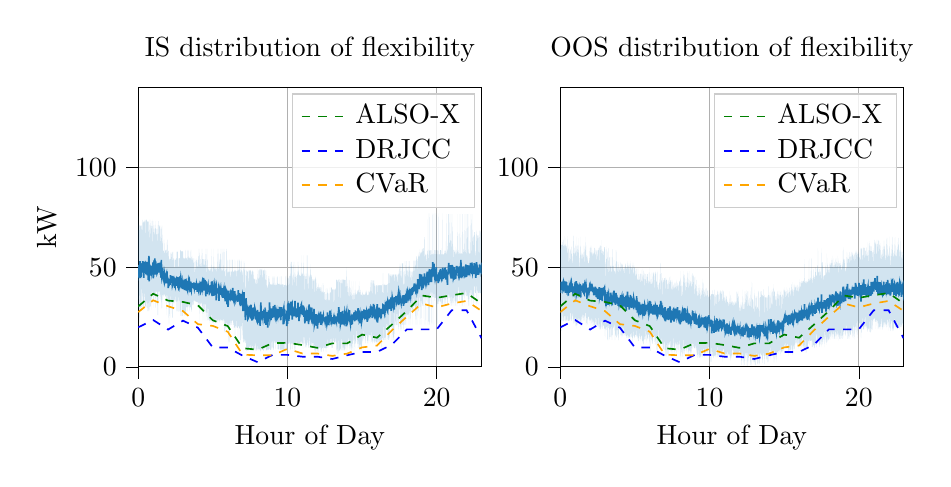
\begin{tikzpicture}

\definecolor{darkgray176}{RGB}{176,176,176}
\definecolor{green}{RGB}{0,128,0}
\definecolor{lightgray204}{RGB}{204,204,204}
\definecolor{orange}{RGB}{255,165,0}
\definecolor{steelblue31119180}{RGB}{31,119,180}

\begin{groupplot}[group style={group size=2 by 1}]
\nextgroupplot[
legend cell align={left},
legend style={fill opacity=0.8, draw opacity=1, text opacity=1, draw=lightgray204},
tick align=outside,
tick pos=left,
title={IS distribution of flexibility},
width=0.49\textwidth,
x grid style={darkgray176},
xlabel={Hour of Day},
xmajorgrids,
xmin=0, xmax=23,
xtick style={color=black},
y grid style={darkgray176},
ylabel={kW},
ymajorgrids,
ymin=0, ymax=139.944507818995,
ytick style={color=black}
]
\path [fill=steelblue31119180, fill opacity=0.2]
(axis cs:0,67.2360368810227)
--(axis cs:0,29.4917446709432)
--(axis cs:0.0166666666666667,29.4917446709432)
--(axis cs:0.0333333333333333,37.7026392795607)
--(axis cs:0.05,36.1543248766068)
--(axis cs:0.0666666666666667,22.2194952500217)
--(axis cs:0.0833333333333333,22.2194952500217)
--(axis cs:0.1,36.9623525900425)
--(axis cs:0.116666666666667,36.9623525900425)
--(axis cs:0.133333333333333,30.0705544461188)
--(axis cs:0.15,30.299772384379)
--(axis cs:0.166666666666667,28.0075930017773)
--(axis cs:0.183333333333333,28.0075930017773)
--(axis cs:0.2,36.9623525900425)
--(axis cs:0.216666666666667,28.0075930017773)
--(axis cs:0.233333333333333,37.7026392795607)
--(axis cs:0.25,43.3948640347184)
--(axis cs:0.266666666666667,39.6566914415438)
--(axis cs:0.283333333333333,28.0075930017773)
--(axis cs:0.3,38.7209995358274)
--(axis cs:0.316666666666667,36.9623525900425)
--(axis cs:0.333333333333333,30.299772384379)
--(axis cs:0.35,36.9623525900425)
--(axis cs:0.366666666666667,30.0705544461188)
--(axis cs:0.383333333333333,28.0075930017773)
--(axis cs:0.4,30.299772384379)
--(axis cs:0.416666666666667,37.7026392795607)
--(axis cs:0.433333333333333,36.7331346517824)
--(axis cs:0.45,36.9623525900425)
--(axis cs:0.466666666666667,30.299772384379)
--(axis cs:0.483333333333333,30.299772384379)
--(axis cs:0.5,30.299772384379)
--(axis cs:0.516666666666667,30.0705544461188)
--(axis cs:0.533333333333333,39.6566914415438)
--(axis cs:0.55,30.0705544461188)
--(axis cs:0.566666666666667,36.9623525900425)
--(axis cs:0.583333333333333,30.299772384379)
--(axis cs:0.6,28.0075930017773)
--(axis cs:0.616666666666667,39.9342371674162)
--(axis cs:0.633333333333333,30.299772384379)
--(axis cs:0.65,28.0075930017773)
--(axis cs:0.666666666666667,28.0075930017773)
--(axis cs:0.683333333333333,30.299772384379)
--(axis cs:0.7,28.0075930017773)
--(axis cs:0.716666666666667,39.6566914415438)
--(axis cs:0.733333333333333,28.0075930017773)
--(axis cs:0.75,30.0705544461188)
--(axis cs:0.766666666666667,37.7026392795607)
--(axis cs:0.783333333333333,30.0705544461188)
--(axis cs:0.8,30.299772384379)
--(axis cs:0.816666666666667,30.299772384379)
--(axis cs:0.833333333333333,30.299772384379)
--(axis cs:0.85,37.7026392795607)
--(axis cs:0.866666666666667,37.7026392795607)
--(axis cs:0.883333333333333,28.5690369733892)
--(axis cs:0.9,36.7892790489436)
--(axis cs:0.916666666666667,37.9148212030345)
--(axis cs:0.933333333333333,36.7892790489436)
--(axis cs:0.95,37.9148212030345)
--(axis cs:0.966666666666667,37.9148212030345)
--(axis cs:0.983333333333333,37.8936030106871)
--(axis cs:1,37.1015277682954)
--(axis cs:1.01666666666667,29.6756371286171)
--(axis cs:1.03333333333333,37.1015277682954)
--(axis cs:1.05,37.1015277682954)
--(axis cs:1.06666666666667,37.1015277682954)
--(axis cs:1.08333333333333,37.1015277682954)
--(axis cs:1.1,36.3589387043276)
--(axis cs:1.11666666666667,37.8936030106871)
--(axis cs:1.13333333333333,29.6756371286171)
--(axis cs:1.15,29.6756371286171)
--(axis cs:1.16666666666667,39.4470434672187)
--(axis cs:1.18333333333333,37.9148212030345)
--(axis cs:1.2,37.7026392795607)
--(axis cs:1.21666666666667,37.7026392795607)
--(axis cs:1.23333333333333,37.7026392795607)
--(axis cs:1.25,37.7026392795607)
--(axis cs:1.26666666666667,25.894025043117)
--(axis cs:1.28333333333333,25.894025043117)
--(axis cs:1.3,39.4470434672187)
--(axis cs:1.31666666666667,36.5217778559163)
--(axis cs:1.33333333333333,25.894025043117)
--(axis cs:1.35,37.8936030106871)
--(axis cs:1.36666666666667,37.7026392795607)
--(axis cs:1.38333333333333,37.7026392795607)
--(axis cs:1.4,37.7026392795607)
--(axis cs:1.41666666666667,37.8936030106871)
--(axis cs:1.43333333333333,37.8936030106871)
--(axis cs:1.45,34.0622068895613)
--(axis cs:1.46666666666667,37.9148212030345)
--(axis cs:1.48333333333333,37.9148212030345)
--(axis cs:1.5,33.2453887049169)
--(axis cs:1.51666666666667,36.4109976020351)
--(axis cs:1.53333333333333,32.3685988582758)
--(axis cs:1.55,39.9587467145356)
--(axis cs:1.56666666666667,29.3920271357896)
--(axis cs:1.58333333333333,29.3920271357896)
--(axis cs:1.6,29.7806940349754)
--(axis cs:1.61666666666667,35.9828463165765)
--(axis cs:1.63333333333333,35.9828463165765)
--(axis cs:1.65,36.6719743478656)
--(axis cs:1.66666666666667,35.5941794173907)
--(axis cs:1.68333333333333,35.1901317247859)
--(axis cs:1.7,36.2230324671935)
--(axis cs:1.71666666666667,36.6719743478656)
--(axis cs:1.73333333333333,36.2230324671935)
--(axis cs:1.75,36.6719743478656)
--(axis cs:1.76666666666667,36.2230324671935)
--(axis cs:1.78333333333333,36.2230324671935)
--(axis cs:1.8,35.1901317247859)
--(axis cs:1.81666666666667,35.1901317247859)
--(axis cs:1.83333333333333,36.2230324671935)
--(axis cs:1.85,35.1901317247859)
--(axis cs:1.86666666666667,36.6719743478656)
--(axis cs:1.88333333333333,25.894025043117)
--(axis cs:1.9,37.7821115232653)
--(axis cs:1.91666666666667,36.2230324671935)
--(axis cs:1.93333333333333,35.9243123120131)
--(axis cs:1.95,33.2358309153895)
--(axis cs:1.96666666666667,36.7492107808576)
--(axis cs:1.98333333333333,36.2230324671935)
--(axis cs:2,33.2358309153895)
--(axis cs:2.01666666666667,21.6662553429586)
--(axis cs:2.03333333333333,36.2230324671935)
--(axis cs:2.05,32.0788733581464)
--(axis cs:2.06666666666667,37.8233303679449)
--(axis cs:2.08333333333333,21.6662553429586)
--(axis cs:2.1,32.0788733581464)
--(axis cs:2.11666666666667,33.2358309153895)
--(axis cs:2.13333333333333,24.6347017926798)
--(axis cs:2.15,33.2358309153895)
--(axis cs:2.16666666666667,35.9243123120131)
--(axis cs:2.18333333333333,36.2230324671935)
--(axis cs:2.2,32.3757180031185)
--(axis cs:2.21666666666667,36.2230324671935)
--(axis cs:2.23333333333333,32.3757180031185)
--(axis cs:2.25,35.9243123120131)
--(axis cs:2.26666666666667,24.6347017926798)
--(axis cs:2.28333333333333,24.6347017926798)
--(axis cs:2.3,24.6347017926798)
--(axis cs:2.31666666666667,35.9243123120131)
--(axis cs:2.33333333333333,31.8792698468649)
--(axis cs:2.35,33.2358309153895)
--(axis cs:2.36666666666667,31.8792698468649)
--(axis cs:2.38333333333333,33.100174808537)
--(axis cs:2.4,35.3029894109232)
--(axis cs:2.41666666666667,31.8792698468649)
--(axis cs:2.43333333333333,38.0245027482229)
--(axis cs:2.45,33.2358309153895)
--(axis cs:2.46666666666667,35.5326736882047)
--(axis cs:2.48333333333333,35.3029894109232)
--(axis cs:2.5,32.6774855741525)
--(axis cs:2.51666666666667,35.9243123120131)
--(axis cs:2.53333333333333,33.2358309153895)
--(axis cs:2.55,32.6774855741525)
--(axis cs:2.56666666666667,33.2358309153895)
--(axis cs:2.58333333333333,27.6523775030204)
--(axis cs:2.6,33.2358309153895)
--(axis cs:2.61666666666667,33.2358309153895)
--(axis cs:2.63333333333333,33.2358309153895)
--(axis cs:2.65,27.6523775030204)
--(axis cs:2.66666666666667,27.6523775030204)
--(axis cs:2.68333333333333,27.6523775030204)
--(axis cs:2.7,35.3029894109232)
--(axis cs:2.71666666666667,35.5326736882047)
--(axis cs:2.73333333333333,33.2358309153895)
--(axis cs:2.75,27.6523775030204)
--(axis cs:2.76666666666667,35.3029894109232)
--(axis cs:2.78333333333333,33.2358309153895)
--(axis cs:2.8,32.9438524496541)
--(axis cs:2.81666666666667,28.4031511522827)
--(axis cs:2.83333333333333,25.5629684802893)
--(axis cs:2.85,27.6523775030204)
--(axis cs:2.86666666666667,36.1539965892946)
--(axis cs:2.88333333333333,32.4685446718794)
--(axis cs:2.9,32.4685446718794)
--(axis cs:2.91666666666667,25.5629684802893)
--(axis cs:2.93333333333333,25.5629684802893)
--(axis cs:2.95,27.6523775030204)
--(axis cs:2.96666666666667,27.4434366007473)
--(axis cs:2.98333333333333,25.5629684802893)
--(axis cs:3,27.4434366007473)
--(axis cs:3.01666666666667,27.6523775030204)
--(axis cs:3.03333333333333,27.6523775030204)
--(axis cs:3.05,27.6523775030204)
--(axis cs:3.06666666666667,27.4434366007473)
--(axis cs:3.08333333333333,27.6523775030204)
--(axis cs:3.1,25.5629684802893)
--(axis cs:3.11666666666667,32.8591060888288)
--(axis cs:3.13333333333333,27.6523775030204)
--(axis cs:3.15,27.6523775030204)
--(axis cs:3.16666666666667,27.6523775030204)
--(axis cs:3.18333333333333,27.4434366007473)
--(axis cs:3.2,25.5629684802893)
--(axis cs:3.21666666666667,32.8591060888288)
--(axis cs:3.23333333333333,29.9369253682925)
--(axis cs:3.25,29.9369253682925)
--(axis cs:3.26666666666667,29.9369253682925)
--(axis cs:3.28333333333333,32.5668880167751)
--(axis cs:3.3,27.6523775030204)
--(axis cs:3.31666666666667,32.5668880167751)
--(axis cs:3.33333333333333,29.9369253682925)
--(axis cs:3.35,33.2358309153895)
--(axis cs:3.36666666666667,32.9059403606798)
--(axis cs:3.38333333333333,29.9369253682925)
--(axis cs:3.4,32.8591060888288)
--(axis cs:3.41666666666667,32.5668880167751)
--(axis cs:3.43333333333333,27.6523775030204)
--(axis cs:3.45,32.8591060888288)
--(axis cs:3.46666666666667,29.9369253682925)
--(axis cs:3.48333333333333,29.7084705817653)
--(axis cs:3.5,29.9369253682925)
--(axis cs:3.51666666666667,29.9369253682925)
--(axis cs:3.53333333333333,30.8027176707672)
--(axis cs:3.55,27.6523775030204)
--(axis cs:3.56666666666667,33.1981584327334)
--(axis cs:3.58333333333333,27.6523775030204)
--(axis cs:3.6,32.8591060888288)
--(axis cs:3.61666666666667,32.8591060888288)
--(axis cs:3.63333333333333,30.8027176707672)
--(axis cs:3.65,32.6534672470226)
--(axis cs:3.66666666666667,30.8027176707672)
--(axis cs:3.68333333333333,33.1981584327334)
--(axis cs:3.7,30.8027176707672)
--(axis cs:3.71666666666667,33.1981584327334)
--(axis cs:3.73333333333333,33.2358309153895)
--(axis cs:3.75,33.785120355919)
--(axis cs:3.76666666666667,32.8591060888288)
--(axis cs:3.78333333333333,33.2358309153895)
--(axis cs:3.8,33.8461525159779)
--(axis cs:3.81666666666667,32.718968592354)
--(axis cs:3.83333333333333,32.718968592354)
--(axis cs:3.85,32.718968592354)
--(axis cs:3.86666666666667,34.1193302793675)
--(axis cs:3.88333333333333,32.450075934944)
--(axis cs:3.9,32.5603364694844)
--(axis cs:3.91666666666667,32.8591060888288)
--(axis cs:3.93333333333333,32.8292291268943)
--(axis cs:3.95,32.5603364694844)
--(axis cs:3.96666666666667,32.450075934944)
--(axis cs:3.98333333333333,32.8591060888288)
--(axis cs:4,31.4577311240813)
--(axis cs:4.01666666666667,33.747447873263)
--(axis cs:4.03333333333333,31.4577311240813)
--(axis cs:4.05,32.8591060888288)
--(axis cs:4.06666666666667,31.4577311240813)
--(axis cs:4.08333333333333,33.8461525159779)
--(axis cs:4.1,23.3593500468316)
--(axis cs:4.11666666666667,32.8591060888288)
--(axis cs:4.13333333333333,32.718968592354)
--(axis cs:4.15,31.4577311240813)
--(axis cs:4.16666666666667,32.718968592354)
--(axis cs:4.18333333333333,30.6478930163563)
--(axis cs:4.2,32.8591060888288)
--(axis cs:4.21666666666667,32.718968592354)
--(axis cs:4.23333333333333,31.4577311240813)
--(axis cs:4.25,32.718968592354)
--(axis cs:4.26666666666667,30.6478930163563)
--(axis cs:4.28333333333333,33.747447873263)
--(axis cs:4.3,23.3593500468316)
--(axis cs:4.31666666666667,31.4577311240813)
--(axis cs:4.33333333333333,30.6478930163563)
--(axis cs:4.35,32.8591060888288)
--(axis cs:4.36666666666667,23.3593500468316)
--(axis cs:4.38333333333333,31.4577311240813)
--(axis cs:4.4,31.4577311240813)
--(axis cs:4.41666666666667,31.4577311240813)
--(axis cs:4.43333333333333,23.3593500468316)
--(axis cs:4.45,32.8591060888288)
--(axis cs:4.46666666666667,31.4530101361516)
--(axis cs:4.48333333333333,31.4577311240813)
--(axis cs:4.5,31.4105212447841)
--(axis cs:4.51666666666667,31.0089429517335)
--(axis cs:4.53333333333333,23.3593500468316)
--(axis cs:4.55,31.4530101361516)
--(axis cs:4.56666666666667,23.3593500468316)
--(axis cs:4.58333333333333,31.0089429517335)
--(axis cs:4.6,26.9911994875335)
--(axis cs:4.61666666666667,23.3593500468316)
--(axis cs:4.63333333333333,23.3593500468316)
--(axis cs:4.65,34.7268635785548)
--(axis cs:4.66666666666667,27.0801853747429)
--(axis cs:4.68333333333333,34.6378776913453)
--(axis cs:4.7,24.1602230317169)
--(axis cs:4.71666666666667,23.3593500468316)
--(axis cs:4.73333333333333,24.2492089189263)
--(axis cs:4.75,23.3593500468316)
--(axis cs:4.76666666666667,23.3593500468316)
--(axis cs:4.78333333333333,24.2492089189263)
--(axis cs:4.8,22.024516215805)
--(axis cs:4.81666666666667,23.3593500468316)
--(axis cs:4.83333333333333,23.3593500468316)
--(axis cs:4.85,23.3593500468316)
--(axis cs:4.86666666666667,23.3593500468316)
--(axis cs:4.88333333333333,23.3593500468316)
--(axis cs:4.9,23.3593500468316)
--(axis cs:4.91666666666667,30.2154351190464)
--(axis cs:4.93333333333333,23.225866663729)
--(axis cs:4.95,22.024516215805)
--(axis cs:4.96666666666667,22.024516215805)
--(axis cs:4.98333333333333,24.1602230317169)
--(axis cs:5,24.1602230317169)
--(axis cs:5.01666666666667,22.024516215805)
--(axis cs:5.03333333333333,23.3593500468316)
--(axis cs:5.05,22.024516215805)
--(axis cs:5.06666666666667,24.1602230317169)
--(axis cs:5.08333333333333,23.3593500468316)
--(axis cs:5.1,23.3593500468316)
--(axis cs:5.11666666666667,23.3593500468316)
--(axis cs:5.13333333333333,24.0267396486142)
--(axis cs:5.15,23.225866663729)
--(axis cs:5.16666666666667,23.3593500468316)
--(axis cs:5.18333333333333,23.3593500468316)
--(axis cs:5.2,24.1602230317169)
--(axis cs:5.21666666666667,25.5881611001437)
--(axis cs:5.23333333333333,23.225866663729)
--(axis cs:5.25,22.024516215805)
--(axis cs:5.26666666666667,23.3593500468316)
--(axis cs:5.28333333333333,24.2492089189263)
--(axis cs:5.3,23.225866663729)
--(axis cs:5.31666666666667,23.225866663729)
--(axis cs:5.33333333333333,22.024516215805)
--(axis cs:5.35,23.3593500468316)
--(axis cs:5.36666666666667,24.0267396486142)
--(axis cs:5.38333333333333,24.2492089189263)
--(axis cs:5.4,23.225866663729)
--(axis cs:5.41666666666667,23.3593500468316)
--(axis cs:5.43333333333333,23.3593500468316)
--(axis cs:5.45,24.2492089189263)
--(axis cs:5.46666666666667,22.024516215805)
--(axis cs:5.48333333333333,23.3593500468316)
--(axis cs:5.5,23.3593500468316)
--(axis cs:5.51666666666667,24.1602230317169)
--(axis cs:5.53333333333333,24.2492089189263)
--(axis cs:5.55,23.3593500468316)
--(axis cs:5.56666666666667,23.3593500468316)
--(axis cs:5.58333333333333,24.1602230317169)
--(axis cs:5.6,23.3593500468316)
--(axis cs:5.61666666666667,23.3593500468316)
--(axis cs:5.63333333333333,23.225866663729)
--(axis cs:5.65,24.2492089189263)
--(axis cs:5.66666666666667,23.3593500468316)
--(axis cs:5.68333333333333,22.024516215805)
--(axis cs:5.7,23.3593500468316)
--(axis cs:5.71666666666667,24.1602230317169)
--(axis cs:5.73333333333333,25.5881611001437)
--(axis cs:5.75,23.225866663729)
--(axis cs:5.76666666666667,23.3593500468316)
--(axis cs:5.78333333333333,16.9523046469496)
--(axis cs:5.8,23.225866663729)
--(axis cs:5.81666666666667,16.9523046469496)
--(axis cs:5.83333333333333,22.024516215805)
--(axis cs:5.85,23.225866663729)
--(axis cs:5.86666666666667,19.1535744277441)
--(axis cs:5.88333333333333,23.225866663729)
--(axis cs:5.9,22.024516215805)
--(axis cs:5.91666666666667,24.0267396486142)
--(axis cs:5.93333333333333,19.1535744277441)
--(axis cs:5.95,22.024516215805)
--(axis cs:5.96666666666667,21.0312119365733)
--(axis cs:5.98333333333333,21.0312119365733)
--(axis cs:6,22.024516215805)
--(axis cs:6.01666666666667,21.0312119365733)
--(axis cs:6.03333333333333,12.0914734234885)
--(axis cs:6.05,22.024516215805)
--(axis cs:6.06666666666667,22.024516215805)
--(axis cs:6.08333333333333,21.0312119365733)
--(axis cs:6.1,22.024516215805)
--(axis cs:6.11666666666667,23.225866663729)
--(axis cs:6.13333333333333,12.0914734234885)
--(axis cs:6.15,21.0312119365733)
--(axis cs:6.16666666666667,21.0312119365733)
--(axis cs:6.18333333333333,22.024516215805)
--(axis cs:6.2,23.3593500468316)
--(axis cs:6.21666666666667,23.225866663729)
--(axis cs:6.23333333333333,23.0334353693826)
--(axis cs:6.25,22.024516215805)
--(axis cs:6.26666666666667,21.0312119365733)
--(axis cs:6.28333333333333,29.9929658487343)
--(axis cs:6.3,23.3593500468316)
--(axis cs:6.31666666666667,23.225866663729)
--(axis cs:6.33333333333333,24.1602230317169)
--(axis cs:6.35,23.225866663729)
--(axis cs:6.36666666666667,21.0312119365733)
--(axis cs:6.38333333333333,23.225866663729)
--(axis cs:6.4,22.2325623844973)
--(axis cs:6.41666666666667,19.6067688413599)
--(axis cs:6.43333333333333,23.3593500468316)
--(axis cs:6.45,19.6067688413599)
--(axis cs:6.46666666666667,23.3593500468316)
--(axis cs:6.48333333333333,12.0914734234885)
--(axis cs:6.5,19.6067688413599)
--(axis cs:6.51666666666667,20.4418016655678)
--(axis cs:6.53333333333333,20.4418016655678)
--(axis cs:6.55,20.4418016655678)
--(axis cs:6.56666666666667,19.6067688413599)
--(axis cs:6.58333333333333,23.0681992467017)
--(axis cs:6.6,23.3302349668186)
--(axis cs:6.61666666666667,20.4418016655678)
--(axis cs:6.63333333333333,19.6067688413599)
--(axis cs:6.65,20.4234175523232)
--(axis cs:6.66666666666667,20.4418016655678)
--(axis cs:6.68333333333333,12.0914734234885)
--(axis cs:6.7,30.3513412322678)
--(axis cs:6.71666666666667,20.4418016655678)
--(axis cs:6.73333333333333,20.2579605331211)
--(axis cs:6.75,20.4418016655678)
--(axis cs:6.76666666666667,19.4413118221578)
--(axis cs:6.78333333333333,19.6067688413599)
--(axis cs:6.8,20.4234175523232)
--(axis cs:6.81666666666667,12.0914734234885)
--(axis cs:6.83333333333333,20.2579605331211)
--(axis cs:6.85,12.0914734234885)
--(axis cs:6.86666666666667,20.2579605331211)
--(axis cs:6.88333333333333,20.4234175523232)
--(axis cs:6.9,20.4234175523232)
--(axis cs:6.91666666666667,20.4234175523232)
--(axis cs:6.93333333333333,20.2579605331211)
--(axis cs:6.95,14.2913260246953)
--(axis cs:6.96666666666667,22.4995486749024)
--(axis cs:6.98333333333333,22.7486140239892)
--(axis cs:7,19.4413118221578)
--(axis cs:7.01666666666667,14.2913260246953)
--(axis cs:7.03333333333333,12.648510057156)
--(axis cs:7.05,12.0914734234885)
--(axis cs:7.06666666666667,12.648510057156)
--(axis cs:7.08333333333333,19.4130768481344)
--(axis cs:7.1,14.1270444279414)
--(axis cs:7.11666666666667,12.648510057156)
--(axis cs:7.13333333333333,14.0713407645746)
--(axis cs:7.15,12.0914734234885)
--(axis cs:7.16666666666667,12.0914734234885)
--(axis cs:7.18333333333333,12.0914734234885)
--(axis cs:7.2,11.7772828342865)
--(axis cs:7.21666666666667,17.1731243377292)
--(axis cs:7.23333333333333,8.94956753146855)
--(axis cs:7.25,7.98014290475649)
--(axis cs:7.26666666666667,8.94956753146855)
--(axis cs:7.28333333333333,7.98014290475649)
--(axis cs:7.3,8.85262506879734)
--(axis cs:7.31666666666667,8.85262506879734)
--(axis cs:7.33333333333333,8.94956753146855)
--(axis cs:7.35,7.98014290475649)
--(axis cs:7.36666666666667,8.94956753146855)
--(axis cs:7.38333333333333,7.98014290475649)
--(axis cs:7.4,11.7772828342865)
--(axis cs:7.41666666666667,8.94956753146855)
--(axis cs:7.43333333333333,8.85262506879734)
--(axis cs:7.45,11.7772828342865)
--(axis cs:7.46666666666667,8.94956753146855)
--(axis cs:7.48333333333333,12.5928063937893)
--(axis cs:7.5,12.5928063937893)
--(axis cs:7.51666666666667,7.98014290475649)
--(axis cs:7.53333333333333,8.94956753146855)
--(axis cs:7.55,11.7772828342865)
--(axis cs:7.56666666666667,8.94956753146855)
--(axis cs:7.58333333333333,8.94956753146855)
--(axis cs:7.6,7.98014290475649)
--(axis cs:7.61666666666667,7.98014290475649)
--(axis cs:7.63333333333333,11.7772828342865)
--(axis cs:7.65,8.94956753146855)
--(axis cs:7.66666666666667,12.648510057156)
--(axis cs:7.68333333333333,11.7772828342865)
--(axis cs:7.7,8.85262506879734)
--(axis cs:7.71666666666667,8.94956753146855)
--(axis cs:7.73333333333333,8.94956753146855)
--(axis cs:7.75,7.98014290475649)
--(axis cs:7.76666666666667,8.94956753146855)
--(axis cs:7.78333333333333,8.85262506879734)
--(axis cs:7.8,8.78967793533981)
--(axis cs:7.81666666666667,12.5928063937893)
--(axis cs:7.83333333333333,11.7612938746737)
--(axis cs:7.85,12.648510057156)
--(axis cs:7.86666666666667,8.70872443228148)
--(axis cs:7.88333333333333,7.98014290475649)
--(axis cs:7.9,8.70872443228148)
--(axis cs:7.91666666666667,10.0777655581706)
--(axis cs:7.93333333333333,7.98014290475649)
--(axis cs:7.95,8.78967793533981)
--(axis cs:7.96666666666667,8.78967793533981)
--(axis cs:7.98333333333333,8.70872443228148)
--(axis cs:8,12.0914734234885)
--(axis cs:8.01666666666667,8.78967793533981)
--(axis cs:8.03333333333333,7.98014290475649)
--(axis cs:8.05,10.3108347418833)
--(axis cs:8.06666666666667,8.70872443228148)
--(axis cs:8.08333333333333,8.70872443228148)
--(axis cs:8.1,8.70872443228148)
--(axis cs:8.11666666666667,8.78967793533981)
--(axis cs:8.13333333333333,8.70872443228148)
--(axis cs:8.15,8.78967793533981)
--(axis cs:8.16666666666667,7.98014290475649)
--(axis cs:8.18333333333333,7.6549986394811)
--(axis cs:8.2,8.568121321039)
--(axis cs:8.21666666666667,8.70872443228148)
--(axis cs:8.23333333333333,7.98014290475649)
--(axis cs:8.25,12.2844691795173)
--(axis cs:8.26666666666667,8.63345225618151)
--(axis cs:8.28333333333333,10.1430964933131)
--(axis cs:8.3,8.568121321039)
--(axis cs:8.31666666666667,10.3108347418833)
--(axis cs:8.33333333333333,8.568121321039)
--(axis cs:8.35,8.568121321039)
--(axis cs:8.36666666666667,8.63345225618151)
--(axis cs:8.38333333333333,8.63345225618151)
--(axis cs:8.4,7.98014290475649)
--(axis cs:8.41666666666667,7.98014290475649)
--(axis cs:8.43333333333333,10.3108347418833)
--(axis cs:8.45,10.3108347418833)
--(axis cs:8.46666666666667,10.1430964933131)
--(axis cs:8.48333333333333,8.63345225618151)
--(axis cs:8.5,10.1430964933131)
--(axis cs:8.51666666666667,10.1430964933131)
--(axis cs:8.53333333333333,13.2087393802349)
--(axis cs:8.55,8.63345225618151)
--(axis cs:8.56666666666667,7.98014290475649)
--(axis cs:8.58333333333333,8.63345225618151)
--(axis cs:8.6,8.63345225618151)
--(axis cs:8.61666666666667,8.35855086958254)
--(axis cs:8.63333333333333,10.3108347418833)
--(axis cs:8.65,8.63345225618151)
--(axis cs:8.66666666666667,8.35855086958254)
--(axis cs:8.68333333333333,8.35855086958254)
--(axis cs:8.7,8.63345225618151)
--(axis cs:8.71666666666667,8.60596211752161)
--(axis cs:8.73333333333333,10.1430964933131)
--(axis cs:8.75,8.35855086958254)
--(axis cs:8.76666666666667,10.1430964933131)
--(axis cs:8.78333333333333,8.63345225618151)
--(axis cs:8.8,13.2087393802349)
--(axis cs:8.81666666666667,10.3108347418833)
--(axis cs:8.83333333333333,8.63345225618151)
--(axis cs:8.85,8.60596211752161)
--(axis cs:8.86666666666667,8.35855086958254)
--(axis cs:8.88333333333333,8.60596211752161)
--(axis cs:8.9,8.60596211752161)
--(axis cs:8.91666666666667,13.0135109930048)
--(axis cs:8.93333333333333,8.63345225618151)
--(axis cs:8.95,13.2888237100968)
--(axis cs:8.96666666666667,15.4226628429333)
--(axis cs:8.98333333333333,8.63345225618151)
--(axis cs:9,13.8035105586078)
--(axis cs:9.01666666666667,13.2590145897053)
--(axis cs:9.03333333333333,8.63345225618151)
--(axis cs:9.05,13.2865047283652)
--(axis cs:9.06666666666667,8.63345225618151)
--(axis cs:9.08333333333333,8.60596211752161)
--(axis cs:9.1,12.9734047110754)
--(axis cs:9.11666666666667,12.0443950154042)
--(axis cs:9.13333333333333,12.9734047110754)
--(axis cs:9.15,12.8805037415083)
--(axis cs:9.16666666666667,12.9734047110754)
--(axis cs:9.18333333333333,12.0443950154042)
--(axis cs:9.2,12.8805037415083)
--(axis cs:9.21666666666667,8.63345225618151)
--(axis cs:9.23333333333333,12.9734047110754)
--(axis cs:9.25,12.9734047110754)
--(axis cs:9.26666666666667,11.7033007394819)
--(axis cs:9.28333333333333,12.539409465586)
--(axis cs:9.3,12.0443950154042)
--(axis cs:9.31666666666667,8.63345225618151)
--(axis cs:9.33333333333333,12.0443950154042)
--(axis cs:9.35,11.7033007394819)
--(axis cs:9.36666666666667,11.7033007394819)
--(axis cs:9.38333333333333,8.63345225618151)
--(axis cs:9.4,12.0443950154042)
--(axis cs:9.41666666666667,8.63345225618151)
--(axis cs:9.43333333333333,11.8829378635147)
--(axis cs:9.45,11.5579893027814)
--(axis cs:9.46666666666667,11.5344971646062)
--(axis cs:9.48333333333333,8.63345225618151)
--(axis cs:9.5,11.8829378635147)
--(axis cs:9.51666666666667,8.60996011800633)
--(axis cs:9.53333333333333,8.60996011800633)
--(axis cs:9.55,8.39853087442975)
--(axis cs:9.56666666666667,8.63345225618151)
--(axis cs:9.58333333333333,8.60996011800633)
--(axis cs:9.6,12.0282493002152)
--(axis cs:9.61666666666667,8.63345225618151)
--(axis cs:9.63333333333333,8.63345225618151)
--(axis cs:9.65,11.8829378635147)
--(axis cs:9.66666666666667,8.60996011800633)
--(axis cs:9.68333333333333,8.63345225618151)
--(axis cs:9.7,11.5579893027814)
--(axis cs:9.71666666666667,8.60996011800633)
--(axis cs:9.73333333333333,8.63345225618151)
--(axis cs:9.75,11.8829378635147)
--(axis cs:9.76666666666667,8.63345225618151)
--(axis cs:9.78333333333333,12.0282493002152)
--(axis cs:9.8,11.5579893027814)
--(axis cs:9.81666666666667,8.60996011800633)
--(axis cs:9.83333333333333,8.39853087442975)
--(axis cs:9.85,11.8829378635147)
--(axis cs:9.86666666666667,11.5344971646062)
--(axis cs:9.88333333333333,11.5579893027814)
--(axis cs:9.9,8.39853087442975)
--(axis cs:9.91666666666667,8.39853087442975)
--(axis cs:9.93333333333333,8.63345225618151)
--(axis cs:9.95,8.39853087442975)
--(axis cs:9.96666666666667,8.63345225618151)
--(axis cs:9.98333333333333,11.5579893027814)
--(axis cs:10,8.39853087442975)
--(axis cs:10.0166666666667,11.8829378635147)
--(axis cs:10.0333333333333,12.0282493002152)
--(axis cs:10.05,12.0282493002152)
--(axis cs:10.0666666666667,11.5344971646062)
--(axis cs:10.0833333333333,11.5344971646062)
--(axis cs:10.1,11.8829378635147)
--(axis cs:10.1166666666667,11.8829378635147)
--(axis cs:10.1333333333333,12.711487294508)
--(axis cs:10.15,12.7856086588529)
--(axis cs:10.1666666666667,11.8829378635147)
--(axis cs:10.1833333333333,8.39853087442975)
--(axis cs:10.2,11.5344971646062)
--(axis cs:10.2166666666667,12.0282493002152)
--(axis cs:10.2333333333333,8.39853087442975)
--(axis cs:10.25,11.5344971646062)
--(axis cs:10.2666666666667,12.0282493002152)
--(axis cs:10.2833333333333,12.0282493002152)
--(axis cs:10.3,11.8829378635147)
--(axis cs:10.3166666666667,8.39853087442975)
--(axis cs:10.3333333333333,11.8829378635147)
--(axis cs:10.35,11.8829378635147)
--(axis cs:10.3666666666667,11.5344971646062)
--(axis cs:10.3833333333333,11.8829378635147)
--(axis cs:10.4,11.8829378635147)
--(axis cs:10.4166666666667,12.0282493002152)
--(axis cs:10.4333333333333,11.5344971646062)
--(axis cs:10.45,12.0282493002152)
--(axis cs:10.4666666666667,8.39853087442975)
--(axis cs:10.4833333333333,8.39853087442975)
--(axis cs:10.5,12.5949967462494)
--(axis cs:10.5166666666667,8.39853087442975)
--(axis cs:10.5333333333333,11.8829378635147)
--(axis cs:10.55,12.0282493002152)
--(axis cs:10.5666666666667,12.0443950154042)
--(axis cs:10.5833333333333,11.5344971646062)
--(axis cs:10.6,12.0282493002152)
--(axis cs:10.6166666666667,12.5399365731649)
--(axis cs:10.6333333333333,13.4169748452884)
--(axis cs:10.65,12.0282493002152)
--(axis cs:10.6666666666667,11.8829378635147)
--(axis cs:10.6833333333333,12.0282493002152)
--(axis cs:10.7,12.0443950154042)
--(axis cs:10.7166666666667,12.0443950154042)
--(axis cs:10.7333333333333,12.0282493002152)
--(axis cs:10.75,11.8829378635147)
--(axis cs:10.7666666666667,11.8829378635147)
--(axis cs:10.7833333333333,12.0282493002152)
--(axis cs:10.8,11.8829378635147)
--(axis cs:10.8166666666667,12.0443950154042)
--(axis cs:10.8333333333333,11.7560138384262)
--(axis cs:10.85,13.5083057451817)
--(axis cs:10.8666666666667,12.0443950154042)
--(axis cs:10.8833333333333,13.3619146722039)
--(axis cs:10.9,12.0443950154042)
--(axis cs:10.9166666666667,11.7560138384262)
--(axis cs:10.9333333333333,13.5083057451817)
--(axis cs:10.95,13.5083057451817)
--(axis cs:10.9666666666667,11.7560138384262)
--(axis cs:10.9833333333333,11.7560138384262)
--(axis cs:11,12.0443950154042)
--(axis cs:11.0166666666667,9.16058324562402)
--(axis cs:11.0333333333333,16.8091484458892)
--(axis cs:11.05,9.16058324562402)
--(axis cs:11.0666666666667,13.3619146722039)
--(axis cs:11.0833333333333,17.0975296228672)
--(axis cs:11.1,11.7945928418351)
--(axis cs:11.1166666666667,18.8464673714007)
--(axis cs:11.1333333333333,13.5083057451817)
--(axis cs:11.15,13.3619146722039)
--(axis cs:11.1666666666667,9.54637327971365)
--(axis cs:11.1833333333333,10.9516232166614)
--(axis cs:11.2,13.5083057451817)
--(axis cs:11.2166666666667,9.54637327971365)
--(axis cs:11.2333333333333,10.8110982229666)
--(axis cs:11.25,9.54637327971365)
--(axis cs:11.2666666666667,10.9516232166614)
--(axis cs:11.2833333333333,10.9516232166614)
--(axis cs:11.3,10.9516232166614)
--(axis cs:11.3166666666667,10.9516232166614)
--(axis cs:11.3333333333333,13.2526374923296)
--(axis cs:11.35,13.5083057451817)
--(axis cs:11.3666666666667,13.5083057451817)
--(axis cs:11.3833333333333,10.9516232166614)
--(axis cs:11.4,10.9516232166614)
--(axis cs:11.4166666666667,9.54637327971365)
--(axis cs:11.4333333333333,9.54637327971365)
--(axis cs:11.45,16.2159077436373)
--(axis cs:11.4666666666667,18.9928584443784)
--(axis cs:11.4833333333333,10.8110982229666)
--(axis cs:11.5,10.8110982229666)
--(axis cs:11.5166666666667,10.8110982229666)
--(axis cs:11.5333333333333,9.54637327971365)
--(axis cs:11.55,10.8110982229666)
--(axis cs:11.5666666666667,13.2526374923296)
--(axis cs:11.5833333333333,9.54637327971365)
--(axis cs:11.6,10.9516232166614)
--(axis cs:11.6166666666667,13.2526374923296)
--(axis cs:11.6333333333333,13.2526374923296)
--(axis cs:11.65,9.54637327971365)
--(axis cs:11.6666666666667,13.5083057451817)
--(axis cs:11.6833333333333,10.8110982229666)
--(axis cs:11.7,15.9602394907853)
--(axis cs:11.7166666666667,9.3405979284176)
--(axis cs:11.7333333333333,16.2159077436373)
--(axis cs:11.75,9.3405979284176)
--(axis cs:11.7666666666667,9.54637327971365)
--(axis cs:11.7833333333333,13.5083057451817)
--(axis cs:11.8,9.54637327971365)
--(axis cs:11.8166666666667,7.48861976675316)
--(axis cs:11.8333333333333,9.3405979284176)
--(axis cs:11.85,9.3405979284176)
--(axis cs:11.8666666666667,9.54637327971365)
--(axis cs:11.8833333333333,7.48861976675316)
--(axis cs:11.9,7.48861976675316)
--(axis cs:11.9166666666667,13.1121124986349)
--(axis cs:11.9333333333333,7.48861976675316)
--(axis cs:11.95,9.54637327971365)
--(axis cs:11.9666666666667,9.54637327971365)
--(axis cs:11.9833333333333,9.54637327971365)
--(axis cs:12,7.48861976675316)
--(axis cs:12.0166666666667,9.54637327971365)
--(axis cs:12.0333333333333,9.54637327971365)
--(axis cs:12.05,7.48861976675316)
--(axis cs:12.0666666666667,7.48861976675316)
--(axis cs:12.0833333333333,9.54637327971365)
--(axis cs:12.1,9.54637327971365)
--(axis cs:12.1166666666667,10.1893321527151)
--(axis cs:12.1333333333333,9.3405979284176)
--(axis cs:12.15,10.986692766188)
--(axis cs:12.1666666666667,9.3405979284176)
--(axis cs:12.1833333333333,10.8426608175406)
--(axis cs:12.2,9.54637327971365)
--(axis cs:12.2166666666667,10.986692766188)
--(axis cs:12.2333333333333,7.48861976675316)
--(axis cs:12.25,7.48861976675316)
--(axis cs:12.2666666666667,10.8426608175406)
--(axis cs:12.2833333333333,7.48861976675316)
--(axis cs:12.3,9.54637327971365)
--(axis cs:12.3166666666667,9.54637327971365)
--(axis cs:12.3333333333333,9.3405979284176)
--(axis cs:12.35,9.54637327971365)
--(axis cs:12.3666666666667,9.3405979284176)
--(axis cs:12.3833333333333,10.8426608175406)
--(axis cs:12.4,9.3405979284176)
--(axis cs:12.4166666666667,7.48861976675316)
--(axis cs:12.4333333333333,10.986692766188)
--(axis cs:12.45,10.8426608175406)
--(axis cs:12.4666666666667,9.3405979284176)
--(axis cs:12.4833333333333,9.3405979284176)
--(axis cs:12.5,9.54637327971365)
--(axis cs:12.5166666666667,9.54637327971365)
--(axis cs:12.5333333333333,9.54637327971365)
--(axis cs:12.55,9.3405979284176)
--(axis cs:12.5666666666667,9.54637327971365)
--(axis cs:12.5833333333333,7.48861976675316)
--(axis cs:12.6,10.986692766188)
--(axis cs:12.6166666666667,9.54637327971365)
--(axis cs:12.6333333333333,9.3405979284176)
--(axis cs:12.65,9.3405979284176)
--(axis cs:12.6666666666667,9.54637327971365)
--(axis cs:12.6833333333333,14.1953364264848)
--(axis cs:12.7,14.55185238874)
--(axis cs:12.7166666666667,10.8426608175406)
--(axis cs:12.7333333333333,10.986692766188)
--(axis cs:12.75,16.1524268445562)
--(axis cs:12.7666666666667,9.54637327971365)
--(axis cs:12.7833333333333,10.8426608175406)
--(axis cs:12.8,10.8426608175406)
--(axis cs:12.8166666666667,10.986692766188)
--(axis cs:12.8333333333333,10.8426608175406)
--(axis cs:12.85,10.8426608175406)
--(axis cs:12.8666666666667,10.986692766188)
--(axis cs:12.8833333333333,10.8426608175406)
--(axis cs:12.9,14.1953364264848)
--(axis cs:12.9166666666667,14.1953364264848)
--(axis cs:12.9333333333333,14.1953364264848)
--(axis cs:12.95,9.54637327971365)
--(axis cs:12.9666666666667,10.8426608175406)
--(axis cs:12.9833333333333,10.986692766188)
--(axis cs:13,13.0546039219083)
--(axis cs:13.0166666666667,9.54637327971365)
--(axis cs:13.0333333333333,9.54637327971365)
--(axis cs:13.05,14.4021275420568)
--(axis cs:13.0666666666667,13.0546039219083)
--(axis cs:13.0833333333333,14.55185238874)
--(axis cs:13.1,14.4021275420568)
--(axis cs:13.1166666666667,13.0546039219083)
--(axis cs:13.1333333333333,12.3826312841683)
--(axis cs:13.15,14.55185238874)
--(axis cs:13.1666666666667,12.3826312841683)
--(axis cs:13.1833333333333,14.55185238874)
--(axis cs:13.2,14.4021275420568)
--(axis cs:13.2166666666667,12.3826312841683)
--(axis cs:13.2333333333333,13.0546039219083)
--(axis cs:13.25,13.0546039219083)
--(axis cs:13.2666666666667,12.3826312841683)
--(axis cs:13.2833333333333,8.32399101069401)
--(axis cs:13.3,13.9290662509354)
--(axis cs:13.3166666666667,6.33487754450831)
--(axis cs:13.3333333333333,6.33487754450831)
--(axis cs:13.35,8.12507966407544)
--(axis cs:13.3666666666667,19.7354451506645)
--(axis cs:13.3833333333333,8.12507966407544)
--(axis cs:13.4,8.12507966407544)
--(axis cs:13.4166666666667,6.33487754450831)
--(axis cs:13.4333333333333,14.55185238874)
--(axis cs:13.45,13.7301549043168)
--(axis cs:13.4666666666667,8.32399101069401)
--(axis cs:13.4833333333333,8.32399101069401)
--(axis cs:13.5,8.12507966407544)
--(axis cs:13.5166666666667,8.32399101069401)
--(axis cs:13.5333333333333,13.9290662509354)
--(axis cs:13.55,8.21469797096329)
--(axis cs:13.5666666666667,8.32399101069401)
--(axis cs:13.5833333333333,14.55185238874)
--(axis cs:13.6,13.9290662509354)
--(axis cs:13.6166666666667,13.9290662509354)
--(axis cs:13.6333333333333,8.31306170672094)
--(axis cs:13.65,8.32399101069401)
--(axis cs:13.6666666666667,8.31306170672094)
--(axis cs:13.6833333333333,16.0980528865696)
--(axis cs:13.7,13.9290662509354)
--(axis cs:13.7166666666667,8.21469797096329)
--(axis cs:13.7333333333333,8.32399101069401)
--(axis cs:13.75,13.9290662509354)
--(axis cs:13.7666666666667,8.31306170672094)
--(axis cs:13.7833333333333,15.8213386334266)
--(axis cs:13.8,8.21469797096329)
--(axis cs:13.8166666666667,8.21469797096329)
--(axis cs:13.8333333333333,8.32399101069401)
--(axis cs:13.85,11.78470985731)
--(axis cs:13.8666666666667,11.4386379726484)
--(axis cs:13.8833333333333,11.4386379726484)
--(axis cs:13.9,8.31306170672094)
--(axis cs:13.9166666666667,11.78470985731)
--(axis cs:13.9333333333333,8.32399101069401)
--(axis cs:13.95,15.8213386334266)
--(axis cs:13.9666666666667,11.78470985731)
--(axis cs:13.9833333333333,11.78470985731)
--(axis cs:14,11.78470985731)
--(axis cs:14.0166666666667,11.78470985731)
--(axis cs:14.0333333333333,8.21469797096329)
--(axis cs:14.05,13.676008989306)
--(axis cs:14.0666666666667,13.4868790761064)
--(axis cs:14.0833333333333,13.4868790761064)
--(axis cs:14.1,16.0104685466262)
--(axis cs:14.1166666666667,11.78470985731)
--(axis cs:14.1333333333333,11.78470985731)
--(axis cs:14.15,11.78470985731)
--(axis cs:14.1666666666667,8.21469797096329)
--(axis cs:14.1833333333333,11.4277086686753)
--(axis cs:14.2,8.21469797096329)
--(axis cs:14.2166666666667,11.4277086686753)
--(axis cs:14.2333333333333,11.78470985731)
--(axis cs:14.25,11.4277086686753)
--(axis cs:14.2666666666667,8.21469797096329)
--(axis cs:14.2833333333333,8.21469797096329)
--(axis cs:14.3,11.4277086686753)
--(axis cs:14.3166666666667,11.4277086686753)
--(axis cs:14.3333333333333,8.21469797096329)
--(axis cs:14.35,11.4277086686753)
--(axis cs:14.3666666666667,11.78470985731)
--(axis cs:14.3833333333333,11.78470985731)
--(axis cs:14.4,15.8213386334266)
--(axis cs:14.4166666666667,16.269852941884)
--(axis cs:14.4333333333333,16.269852941884)
--(axis cs:14.45,8.21469797096329)
--(axis cs:14.4666666666667,22.0201004250567)
--(axis cs:14.4833333333333,11.4277086686753)
--(axis cs:14.5,8.21469797096329)
--(axis cs:14.5166666666667,15.8213386334266)
--(axis cs:14.5333333333333,11.78470985731)
--(axis cs:14.55,11.78470985731)
--(axis cs:14.5666666666667,15.8213386334266)
--(axis cs:14.5833333333333,9.35238742297895)
--(axis cs:14.6,16.269852941884)
--(axis cs:14.6166666666667,20.1269029548978)
--(axis cs:14.6333333333333,16.269852941884)
--(axis cs:14.65,16.0471006371502)
--(axis cs:14.6666666666667,13.5859766413004)
--(axis cs:14.6833333333333,9.4787973620918)
--(axis cs:14.7,13.5859766413004)
--(axis cs:14.7166666666667,13.5859766413004)
--(axis cs:14.7333333333333,16.0471006371502)
--(axis cs:14.75,9.4787973620918)
--(axis cs:14.7666666666667,9.4787973620918)
--(axis cs:14.7833333333333,13.5859766413004)
--(axis cs:14.8,9.4787973620918)
--(axis cs:14.8166666666667,14.0423298945458)
--(axis cs:14.8333333333333,8.21469797096329)
--(axis cs:14.85,9.35238742297895)
--(axis cs:14.8666666666667,13.5859766413004)
--(axis cs:14.8833333333333,8.21469797096329)
--(axis cs:14.9,9.4787973620918)
--(axis cs:14.9166666666667,13.5859766413004)
--(axis cs:14.9333333333333,9.4787973620918)
--(axis cs:14.95,9.4787973620918)
--(axis cs:14.9666666666667,8.21469797096329)
--(axis cs:14.9833333333333,9.35238742297895)
--(axis cs:15,16.2076029772048)
--(axis cs:15.0166666666667,16.2636279454161)
--(axis cs:15.0333333333333,14.1875567721565)
--(axis cs:15.05,11.7421820645102)
--(axis cs:15.0666666666667,14.4592650730061)
--(axis cs:15.0833333333333,14.4592650730061)
--(axis cs:15.1,14.1875567721565)
--(axis cs:15.1166666666667,20.4723297625329)
--(axis cs:15.1333333333333,16.1900004839958)
--(axis cs:15.15,16.1900004839958)
--(axis cs:15.1666666666667,15.7452186420473)
--(axis cs:15.1833333333333,16.1900004839958)
--(axis cs:15.2,11.7421820645102)
--(axis cs:15.2166666666667,16.2636279454161)
--(axis cs:15.2333333333333,16.2058427278839)
--(axis cs:15.25,11.7421820645102)
--(axis cs:15.2666666666667,16.2076029772048)
--(axis cs:15.2833333333333,16.269852941884)
--(axis cs:15.3,15.7610608859354)
--(axis cs:15.3166666666667,15.8170858541466)
--(axis cs:15.3333333333333,16.2076029772048)
--(axis cs:15.35,11.7421820645102)
--(axis cs:15.3666666666667,16.2076029772048)
--(axis cs:15.3833333333333,11.7421820645102)
--(axis cs:15.4,16.2636279454161)
--(axis cs:15.4166666666667,11.7421820645102)
--(axis cs:15.4333333333333,16.269852941884)
--(axis cs:15.45,16.2076029772048)
--(axis cs:15.4666666666667,16.269852941884)
--(axis cs:15.4833333333333,15.7610608859354)
--(axis cs:15.5,16.2076029772048)
--(axis cs:15.5166666666667,16.2076029772048)
--(axis cs:15.5333333333333,11.7421820645102)
--(axis cs:15.55,16.269852941884)
--(axis cs:15.5666666666667,15.7610608859354)
--(axis cs:15.5833333333333,16.2076029772048)
--(axis cs:15.6,21.4450756767394)
--(axis cs:15.6166666666667,15.8465022056743)
--(axis cs:15.6333333333333,12.5111539421605)
--(axis cs:15.65,12.5965952618994)
--(axis cs:15.6666666666667,15.8465022056743)
--(axis cs:15.6833333333333,11.7421820645102)
--(axis cs:15.7,11.7421820645102)
--(axis cs:15.7166666666667,15.7610608859354)
--(axis cs:15.7333333333333,12.5965952618994)
--(axis cs:15.75,12.5965952618994)
--(axis cs:15.7666666666667,15.8465022056743)
--(axis cs:15.7833333333333,15.8465022056743)
--(axis cs:15.8,16.2076029772048)
--(axis cs:15.8166666666667,12.5221978118117)
--(axis cs:15.8333333333333,11.8526207610221)
--(axis cs:15.85,12.5965952618994)
--(axis cs:15.8666666666667,15.8465022056743)
--(axis cs:15.8833333333333,15.8465022056743)
--(axis cs:15.9,11.8526207610221)
--(axis cs:15.9166666666667,16.2076029772048)
--(axis cs:15.9333333333333,12.5221978118117)
--(axis cs:15.95,12.5965952618994)
--(axis cs:15.9666666666667,12.5221978118117)
--(axis cs:15.9833333333333,11.8526207610221)
--(axis cs:16,9.87272543269653)
--(axis cs:16.0166666666667,21.1974832443967)
--(axis cs:16.0333333333333,12.5965952618994)
--(axis cs:16.05,12.3242082789791)
--(axis cs:16.0666666666667,12.3242082789791)
--(axis cs:16.0833333333333,21.1974832443967)
--(axis cs:16.1,12.5965952618994)
--(axis cs:16.1166666666667,12.5965952618994)
--(axis cs:16.1333333333333,13.4274155888271)
--(axis cs:16.15,20.1025304497493)
--(axis cs:16.1666666666667,9.87272543269653)
--(axis cs:16.1833333333333,13.1550286059068)
--(axis cs:16.2,19.4442503006229)
--(axis cs:16.2166666666667,13.1550286059068)
--(axis cs:16.2333333333333,13.5197289584857)
--(axis cs:16.25,20.1025304497493)
--(axis cs:16.2666666666667,13.1550286059068)
--(axis cs:16.2833333333333,9.87272543269653)
--(axis cs:16.3,20.4297078158056)
--(axis cs:16.3166666666667,13.5197289584857)
--(axis cs:16.3333333333333,14.6042567441655)
--(axis cs:16.35,19.5527030791909)
--(axis cs:16.3666666666667,13.5197289584857)
--(axis cs:16.3833333333333,14.6042567441655)
--(axis cs:16.4,20.1025304497493)
--(axis cs:16.4166666666667,20.1025304497493)
--(axis cs:16.4333333333333,13.5197289584857)
--(axis cs:16.45,19.5527030791909)
--(axis cs:16.4666666666667,13.5197289584857)
--(axis cs:16.4833333333333,13.5197289584857)
--(axis cs:16.5,14.6042567441655)
--(axis cs:16.5166666666667,20.5381605943735)
--(axis cs:16.5333333333333,14.6042567441655)
--(axis cs:16.55,13.5197289584857)
--(axis cs:16.5666666666667,14.4958039655975)
--(axis cs:16.5833333333333,14.6042567441655)
--(axis cs:16.6,21.5527857277552)
--(axis cs:16.6166666666667,21.5527857277552)
--(axis cs:16.6333333333333,20.4297078158056)
--(axis cs:16.65,20.4297078158056)
--(axis cs:16.6666666666667,13.5197289584857)
--(axis cs:16.6833333333333,13.5197289584857)
--(axis cs:16.7,21.5172554794194)
--(axis cs:16.7166666666667,21.1974832443967)
--(axis cs:16.7333333333333,21.1974832443967)
--(axis cs:16.75,13.5197289584857)
--(axis cs:16.7666666666667,26.5349367246897)
--(axis cs:16.7833333333333,13.5197289584857)
--(axis cs:16.8,13.5197289584857)
--(axis cs:16.8166666666667,21.1974832443967)
--(axis cs:16.8333333333333,13.5197289584857)
--(axis cs:16.85,28.6876562923631)
--(axis cs:16.8666666666667,29.3347233779395)
--(axis cs:16.8833333333333,28.6876562923631)
--(axis cs:16.9,21.1974832443967)
--(axis cs:16.9166666666667,27.9386389875665)
--(axis cs:16.9333333333333,21.1974832443967)
--(axis cs:16.95,21.1974832443967)
--(axis cs:16.9666666666667,28.7057079947796)
--(axis cs:16.9833333333333,20.4297078158056)
--(axis cs:17,13.5197289584857)
--(axis cs:17.0166666666667,29.4066197207813)
--(axis cs:17.0333333333333,20.4297078158056)
--(axis cs:17.05,21.1974832443967)
--(axis cs:17.0666666666667,13.5197289584857)
--(axis cs:17.0833333333333,20.4297078158056)
--(axis cs:17.1,13.5197289584857)
--(axis cs:17.1166666666667,20.4297078158056)
--(axis cs:17.1333333333333,13.5197289584857)
--(axis cs:17.15,13.5197289584857)
--(axis cs:17.1666666666667,28.4788246252635)
--(axis cs:17.1833333333333,28.4788246252635)
--(axis cs:17.2,21.1974832443967)
--(axis cs:17.2166666666667,20.4297078158056)
--(axis cs:17.2333333333333,29.2878625564709)
--(axis cs:17.25,21.1974832443967)
--(axis cs:17.2666666666667,29.4066197207813)
--(axis cs:17.2833333333333,28.4788246252635)
--(axis cs:17.3,20.8754360161065)
--(axis cs:17.3166666666667,21.1974832443967)
--(axis cs:17.3333333333333,21.1974832443967)
--(axis cs:17.35,20.8754360161065)
--(axis cs:17.3666666666667,20.8754360161065)
--(axis cs:17.3833333333333,29.4394360875755)
--(axis cs:17.4,28.6152408032576)
--(axis cs:17.4166666666667,20.8754360161065)
--(axis cs:17.4333333333333,17.9770109614947)
--(axis cs:17.45,21.1974832443967)
--(axis cs:17.4666666666667,29.3947440043503)
--(axis cs:17.4833333333333,29.4066197207813)
--(axis cs:17.5,28.4788246252635)
--(axis cs:17.5166666666667,29.2878625564709)
--(axis cs:17.5333333333333,21.1974832443967)
--(axis cs:17.55,17.9770109614947)
--(axis cs:17.5666666666667,20.8754360161065)
--(axis cs:17.5833333333333,21.1974832443967)
--(axis cs:17.6,21.1974832443967)
--(axis cs:17.6166666666667,17.9770109614947)
--(axis cs:17.6333333333333,21.1974832443967)
--(axis cs:17.65,28.0713642917894)
--(axis cs:17.6666666666667,21.1974832443967)
--(axis cs:17.6833333333333,21.1974832443967)
--(axis cs:17.7,21.1974832443967)
--(axis cs:17.7166666666667,29.4147883894446)
--(axis cs:17.7333333333333,21.1974832443967)
--(axis cs:17.75,28.3934115200795)
--(axis cs:17.7666666666667,17.9770109614947)
--(axis cs:17.7833333333333,21.1974832443967)
--(axis cs:17.8,20.8754360161065)
--(axis cs:17.8166666666667,21.1974832443967)
--(axis cs:17.8333333333333,21.1974832443967)
--(axis cs:17.85,28.0516542923042)
--(axis cs:17.8666666666667,29.0788286248703)
--(axis cs:17.8833333333333,21.1974832443967)
--(axis cs:17.9,21.1974832443967)
--(axis cs:17.9166666666667,25.844649595237)
--(axis cs:17.9333333333333,26.361001411997)
--(axis cs:17.95,25.844649595237)
--(axis cs:17.9666666666667,27.8825890042735)
--(axis cs:17.9833333333333,27.8825890042735)
--(axis cs:18,21.1974832443967)
--(axis cs:18.0166666666667,25.844649595237)
--(axis cs:18.0333333333333,25.844649595237)
--(axis cs:18.05,26.361001411997)
--(axis cs:18.0666666666667,26.361001411997)
--(axis cs:18.0833333333333,26.361001411997)
--(axis cs:18.1,26.361001411997)
--(axis cs:18.1166666666667,26.361001411997)
--(axis cs:18.1333333333333,21.1974832443967)
--(axis cs:18.15,21.1974832443967)
--(axis cs:18.1666666666667,26.361001411997)
--(axis cs:18.1833333333333,27.8825890042735)
--(axis cs:18.2,28.0516542923042)
--(axis cs:18.2166666666667,27.8825890042735)
--(axis cs:18.2333333333333,28.0516542923042)
--(axis cs:18.25,21.1974832443967)
--(axis cs:18.2666666666667,26.361001411997)
--(axis cs:18.2833333333333,27.8825890042735)
--(axis cs:18.3,27.3662371875134)
--(axis cs:18.3166666666667,33.5925977041251)
--(axis cs:18.3333333333333,33.5091282944204)
--(axis cs:18.35,28.0516542923042)
--(axis cs:18.3666666666667,34.856298043486)
--(axis cs:18.3833333333333,21.1974832443967)
--(axis cs:18.4,35.0819031554313)
--(axis cs:18.4166666666667,34.1758336683679)
--(axis cs:18.4333333333333,34.1758336683679)
--(axis cs:18.45,28.0516542923042)
--(axis cs:18.4666666666667,28.0516542923042)
--(axis cs:18.4833333333333,33.4904165635771)
--(axis cs:18.5,35.0819031554313)
--(axis cs:18.5166666666667,27.3662371875134)
--(axis cs:18.5333333333333,34.856298043486)
--(axis cs:18.55,28.0516542923042)
--(axis cs:18.5666666666667,21.1974832443967)
--(axis cs:18.5833333333333,28.0516542923042)
--(axis cs:18.6,28.7177348408888)
--(axis cs:18.6166666666667,28.7177348408888)
--(axis cs:18.6333333333333,28.7177348408888)
--(axis cs:18.65,28.7177348408888)
--(axis cs:18.6666666666667,21.1974832443967)
--(axis cs:18.6833333333333,34.856298043486)
--(axis cs:18.7,21.1974832443967)
--(axis cs:18.7166666666667,33.4904165635771)
--(axis cs:18.7333333333333,35.716337944158)
--(axis cs:18.75,34.2424417232263)
--(axis cs:18.7666666666667,28.7177348408888)
--(axis cs:18.7833333333333,27.9657096812396)
--(axis cs:18.8,32.2187013541739)
--(axis cs:18.8166666666667,21.1974832443967)
--(axis cs:18.8333333333333,33.4432811441492)
--(axis cs:18.85,34.9180409543031)
--(axis cs:18.8666666666667,34.9180409543031)
--(axis cs:18.8833333333333,35.0819031554313)
--(axis cs:18.9,32.2187013541739)
--(axis cs:18.9166666666667,21.1974832443967)
--(axis cs:18.9333333333333,33.4432811441492)
--(axis cs:18.95,32.2187013541739)
--(axis cs:18.9666666666667,33.4432811441492)
--(axis cs:18.9833333333333,34.9180409543031)
--(axis cs:19,21.1974832443967)
--(axis cs:19.0166666666667,33.4432811441492)
--(axis cs:19.0333333333333,31.6144854515713)
--(axis cs:19.05,33.4432811441492)
--(axis cs:19.0666666666667,30.5727852308538)
--(axis cs:19.0833333333333,30.5727852308538)
--(axis cs:19.1,35.8525336144198)
--(axis cs:19.1166666666667,35.8118979331215)
--(axis cs:19.1333333333333,35.8118979331215)
--(axis cs:19.15,21.1974832443967)
--(axis cs:19.1666666666667,34.350456464249)
--(axis cs:19.1833333333333,36.302293643824)
--(axis cs:19.2,36.2982300756942)
--(axis cs:19.2166666666667,34.350456464249)
--(axis cs:19.2333333333333,35.8118979331215)
--(axis cs:19.25,34.350456464249)
--(axis cs:19.2666666666667,21.1974832443967)
--(axis cs:19.2833333333333,35.8118979331215)
--(axis cs:19.3,35.8118979331215)
--(axis cs:19.3166666666667,35.8118979331215)
--(axis cs:19.3333333333333,35.8118979331215)
--(axis cs:19.35,21.1974832443967)
--(axis cs:19.3666666666667,34.350456464249)
--(axis cs:19.3833333333333,36.2982300756942)
--(axis cs:19.4,36.4737972455551)
--(axis cs:19.4166666666667,35.8118979331215)
--(axis cs:19.4333333333333,34.350456464249)
--(axis cs:19.45,21.1974832443967)
--(axis cs:19.4666666666667,35.8118979331215)
--(axis cs:19.4833333333333,21.1974832443967)
--(axis cs:19.5,35.8118979331215)
--(axis cs:19.5166666666667,34.9583188719524)
--(axis cs:19.5333333333333,21.1974832443967)
--(axis cs:19.55,34.350456464249)
--(axis cs:19.5666666666667,36.4873006083474)
--(axis cs:19.5833333333333,36.4873006083474)
--(axis cs:19.6,38.3765280129976)
--(axis cs:19.6166666666667,37.3442562081063)
--(axis cs:19.6333333333333,38.2733008325085)
--(axis cs:19.65,21.1974832443967)
--(axis cs:19.6666666666667,36.4873006083474)
--(axis cs:19.6833333333333,36.4873006083474)
--(axis cs:19.7,34.9583188719524)
--(axis cs:19.7166666666667,37.3442562081063)
--(axis cs:19.7333333333333,38.2733008325085)
--(axis cs:19.75,21.1974832443967)
--(axis cs:19.7666666666667,38.1876052725326)
--(axis cs:19.7833333333333,36.4873006083474)
--(axis cs:19.8,34.9583188719524)
--(axis cs:19.8166666666667,37.2585606481304)
--(axis cs:19.8333333333333,36.4873006083474)
--(axis cs:19.85,34.6266864370862)
--(axis cs:19.8666666666667,33.2837661178172)
--(axis cs:19.8833333333333,33.2837661178172)
--(axis cs:19.9,34.9583188719524)
--(axis cs:19.9166666666667,34.6266864370862)
--(axis cs:19.9333333333333,34.6266864370862)
--(axis cs:19.95,36.3012391912213)
--(axis cs:19.9666666666667,34.6266864370862)
--(axis cs:19.9833333333333,21.1974832443967)
--(axis cs:20,30.4964126107777)
--(axis cs:20.0166666666667,30.4964126107777)
--(axis cs:20.0333333333333,21.1974832443967)
--(axis cs:20.05,32.4452230020958)
--(axis cs:20.0666666666667,31.5153300654577)
--(axis cs:20.0833333333333,35.3161977176671)
--(axis cs:20.1,32.66175749002)
--(axis cs:20.1166666666667,36.3012391912213)
--(axis cs:20.1333333333333,31.5153300654577)
--(axis cs:20.15,32.66175749002)
--(axis cs:20.1666666666667,34.6266864370862)
--(axis cs:20.1833333333333,34.6266864370862)
--(axis cs:20.2,34.4301935423796)
--(axis cs:20.2166666666667,32.66175749002)
--(axis cs:20.2333333333333,35.7529773265822)
--(axis cs:20.25,32.66175749002)
--(axis cs:20.2666666666667,32.66175749002)
--(axis cs:20.2833333333333,31.5153300654577)
--(axis cs:20.3,34.4301935423796)
--(axis cs:20.3166666666667,36.3012391912213)
--(axis cs:20.3333333333333,30.7497380973297)
--(axis cs:20.35,32.66175749002)
--(axis cs:20.3666666666667,32.470555550751)
--(axis cs:20.3833333333333,30.7497380973297)
--(axis cs:20.4,36.3012391912213)
--(axis cs:20.4166666666667,30.7497380973297)
--(axis cs:20.4333333333333,36.4873006083474)
--(axis cs:20.45,34.2389916031105)
--(axis cs:20.4666666666667,34.6266864370862)
--(axis cs:20.4833333333333,34.6266864370862)
--(axis cs:20.5,34.6266864370862)
--(axis cs:20.5166666666667,30.7497380973297)
--(axis cs:20.5333333333333,36.3012391912213)
--(axis cs:20.55,36.8451794540622)
--(axis cs:20.5666666666667,36.4873006083474)
--(axis cs:20.5833333333333,34.6266864370862)
--(axis cs:20.6,30.7497380973297)
--(axis cs:20.6166666666667,35.9135443572457)
--(axis cs:20.6333333333333,36.3012391912213)
--(axis cs:20.65,36.4873006083474)
--(axis cs:20.6666666666667,36.3012391912213)
--(axis cs:20.6833333333333,34.6266864370862)
--(axis cs:20.7,30.7497380973297)
--(axis cs:20.7166666666667,30.7497380973297)
--(axis cs:20.7333333333333,34.6266864370862)
--(axis cs:20.75,34.2389916031105)
--(axis cs:20.7666666666667,34.6266864370862)
--(axis cs:20.7833333333333,34.6266864370862)
--(axis cs:20.8,40.8900191204873)
--(axis cs:20.8166666666667,36.4873006083474)
--(axis cs:20.8333333333333,34.2389916031105)
--(axis cs:20.85,36.4873006083474)
--(axis cs:20.8666666666667,36.3012391912213)
--(axis cs:20.8833333333333,34.6266864370862)
--(axis cs:20.9,36.6591180369361)
--(axis cs:20.9166666666667,30.7497380973297)
--(axis cs:20.9333333333333,34.2389916031105)
--(axis cs:20.95,34.2389916031105)
--(axis cs:20.9666666666667,30.7497380973297)
--(axis cs:20.9833333333333,30.7497380973297)
--(axis cs:21,34.6266864370862)
--(axis cs:21.0166666666667,36.3012391912213)
--(axis cs:21.0333333333333,36.4873006083474)
--(axis cs:21.05,30.7497380973297)
--(axis cs:21.0666666666667,34.2389916031105)
--(axis cs:21.0833333333333,34.2389916031105)
--(axis cs:21.1,30.7497380973297)
--(axis cs:21.1166666666667,34.2389916031105)
--(axis cs:21.1333333333333,34.6266864370862)
--(axis cs:21.15,34.6266864370862)
--(axis cs:21.1666666666667,36.3012391912213)
--(axis cs:21.1833333333333,36.8451794540622)
--(axis cs:21.2,34.6266864370862)
--(axis cs:21.2166666666667,30.7497380973297)
--(axis cs:21.2333333333333,34.2389916031105)
--(axis cs:21.25,34.6266864370862)
--(axis cs:21.2666666666667,30.7497380973297)
--(axis cs:21.2833333333333,30.7497380973297)
--(axis cs:21.3,36.3012391912213)
--(axis cs:21.3166666666667,30.7497380973297)
--(axis cs:21.3333333333333,34.6266864370862)
--(axis cs:21.35,40.1260220025026)
--(axis cs:21.3666666666667,34.6266864370862)
--(axis cs:21.3833333333333,30.7497380973297)
--(axis cs:21.4,34.2389916031105)
--(axis cs:21.4166666666667,36.4873006083474)
--(axis cs:21.4333333333333,40.0152778048067)
--(axis cs:21.45,40.0152778048067)
--(axis cs:21.4666666666667,40.40727527108)
--(axis cs:21.4833333333333,36.4873006083474)
--(axis cs:21.5,40.0152778048067)
--(axis cs:21.5166666666667,30.7497380973297)
--(axis cs:21.5333333333333,36.4873006083474)
--(axis cs:21.55,36.4873006083474)
--(axis cs:21.5666666666667,35.9135443572457)
--(axis cs:21.5833333333333,40.3120834196288)
--(axis cs:21.6,35.9135443572457)
--(axis cs:21.6166666666667,35.9009875474962)
--(axis cs:21.6333333333333,35.3858626024795)
--(axis cs:21.65,30.7497380973297)
--(axis cs:21.6666666666667,39.9566464987216)
--(axis cs:21.6833333333333,35.9009875474962)
--(axis cs:21.7,30.7497380973297)
--(axis cs:21.7166666666667,35.3858626024795)
--(axis cs:21.7333333333333,35.3858626024795)
--(axis cs:21.75,30.7497380973297)
--(axis cs:21.7666666666667,39.9566464987216)
--(axis cs:21.7833333333333,35.3858626024795)
--(axis cs:21.8,40.40727527108)
--(axis cs:21.8166666666667,35.3858626024795)
--(axis cs:21.8333333333333,39.9566464987216)
--(axis cs:21.85,30.7497380973297)
--(axis cs:21.8666666666667,40.40727527108)
--(axis cs:21.8833333333333,35.9009875474962)
--(axis cs:21.9,40.7370592875489)
--(axis cs:21.9166666666667,35.9009875474962)
--(axis cs:21.9333333333333,35.9009875474962)
--(axis cs:21.95,39.9566464987216)
--(axis cs:21.9666666666667,39.9566464987216)
--(axis cs:21.9833333333333,35.9009875474962)
--(axis cs:22,35.3858626024795)
--(axis cs:22.0166666666667,35.9009875474962)
--(axis cs:22.0333333333333,35.3858626024795)
--(axis cs:22.05,35.9009875474962)
--(axis cs:22.0666666666667,35.9009875474962)
--(axis cs:22.0833333333333,39.9566464987216)
--(axis cs:22.1,30.7497380973297)
--(axis cs:22.1166666666667,35.9009875474962)
--(axis cs:22.1333333333333,30.7497380973297)
--(axis cs:22.15,40.8204385729076)
--(axis cs:22.1666666666667,30.7497380973297)
--(axis cs:22.1833333333333,35.3858626024795)
--(axis cs:22.2,40.40727527108)
--(axis cs:22.2166666666667,35.9009875474962)
--(axis cs:22.2333333333333,40.40727527108)
--(axis cs:22.25,35.9009875474962)
--(axis cs:22.2666666666667,35.3858626024795)
--(axis cs:22.2833333333333,39.9566464987216)
--(axis cs:22.3,40.40727527108)
--(axis cs:22.3166666666667,30.7497380973297)
--(axis cs:22.3333333333333,35.9009875474962)
--(axis cs:22.35,39.441521553705)
--(axis cs:22.3666666666667,39.9566464987216)
--(axis cs:22.3833333333333,35.3858626024795)
--(axis cs:22.4,35.9009875474962)
--(axis cs:22.4166666666667,35.3858626024795)
--(axis cs:22.4333333333333,35.9009875474962)
--(axis cs:22.45,30.7497380973297)
--(axis cs:22.4666666666667,35.9009875474962)
--(axis cs:22.4833333333333,35.9009875474962)
--(axis cs:22.5,35.3858626024795)
--(axis cs:22.5166666666667,42.982622830242)
--(axis cs:22.5333333333333,40.0718554704838)
--(axis cs:22.55,40.40727527108)
--(axis cs:22.5666666666667,37.0530772651178)
--(axis cs:22.5833333333333,37.0530772651178)
--(axis cs:22.6,40.40727527108)
--(axis cs:22.6166666666667,36.4370894983493)
--(axis cs:22.6333333333333,37.0530772651178)
--(axis cs:22.65,30.8931995974331)
--(axis cs:22.6666666666667,40.0718554704838)
--(axis cs:22.6833333333333,42.1549580902795)
--(axis cs:22.7,40.0718554704838)
--(axis cs:22.7166666666667,38.0076173493957)
--(axis cs:22.7333333333333,38.1136773587599)
--(axis cs:22.75,37.0530772651178)
--(axis cs:22.7666666666667,30.8931995974331)
--(axis cs:22.7833333333333,38.0076173493957)
--(axis cs:22.8,37.0530772651178)
--(axis cs:22.8166666666667,37.0530772651178)
--(axis cs:22.8333333333333,38.0076173493957)
--(axis cs:22.85,38.1136773587599)
--(axis cs:22.8666666666667,37.0530772651178)
--(axis cs:22.8833333333333,37.0530772651178)
--(axis cs:22.9,36.4370894983493)
--(axis cs:22.9166666666667,37.0530772651178)
--(axis cs:22.9333333333333,37.0530772651178)
--(axis cs:22.95,37.0530772651178)
--(axis cs:22.9666666666667,42.3491450701905)
--(axis cs:22.9833333333333,36.4370894983493)
--(axis cs:23,30.8931995974331)
--(axis cs:23.0166666666667,41.9255982990474)
--(axis cs:23.0333333333333,38.1136773587599)
--(axis cs:23.05,38.0550197811847)
--(axis cs:23.0666666666667,36.8637113844506)
--(axis cs:23.0833333333333,38.0550197811847)
--(axis cs:23.1,37.5271015830081)
--(axis cs:23.1166666666667,37.5271015830081)
--(axis cs:23.1333333333333,38.0550197811847)
--(axis cs:23.15,37.5271015830081)
--(axis cs:23.1666666666667,38.0550197811847)
--(axis cs:23.1833333333333,37.5271015830081)
--(axis cs:23.2,36.8637113844506)
--(axis cs:23.2166666666667,38.1136773587599)
--(axis cs:23.2333333333333,30.8931995974331)
--(axis cs:23.25,37.3916295826272)
--(axis cs:23.2666666666667,30.8931995974331)
--(axis cs:23.2833333333333,38.1136773587599)
--(axis cs:23.3,38.1136773587599)
--(axis cs:23.3166666666667,38.1136773587599)
--(axis cs:23.3333333333333,38.1136773587599)
--(axis cs:23.35,40.670236476184)
--(axis cs:23.3666666666667,38.1136773587599)
--(axis cs:23.3833333333333,42.1812542107899)
--(axis cs:23.4,38.1871292364183)
--(axis cs:23.4166666666667,31.7888755867918)
--(axis cs:23.4333333333333,30.8931995974331)
--(axis cs:23.45,31.7888755867918)
--(axis cs:23.4666666666667,30.8931995974331)
--(axis cs:23.4833333333333,31.7888755867918)
--(axis cs:23.5,31.7888755867918)
--(axis cs:23.5166666666667,37.5473038714556)
--(axis cs:23.5333333333333,30.8931995974331)
--(axis cs:23.55,29.478977906953)
--(axis cs:23.5666666666667,30.8931995974331)
--(axis cs:23.5833333333333,30.8931995974331)
--(axis cs:23.6,16.750982692632)
--(axis cs:23.6166666666667,37.4577362725197)
--(axis cs:23.6333333333333,29.478977906953)
--(axis cs:23.65,29.478977906953)
--(axis cs:23.6666666666667,16.750982692632)
--(axis cs:23.6833333333333,30.8931995974331)
--(axis cs:23.7,40.670236476184)
--(axis cs:23.7166666666667,30.8931995974331)
--(axis cs:23.7333333333333,16.750982692632)
--(axis cs:23.75,30.8931995974331)
--(axis cs:23.7666666666667,30.0258291626919)
--(axis cs:23.7833333333333,30.8931995974331)
--(axis cs:23.8,30.8931995974331)
--(axis cs:23.8166666666667,30.8931995974331)
--(axis cs:23.8333333333333,39.6925327883089)
--(axis cs:23.85,30.8931995974331)
--(axis cs:23.8666666666667,22.2194952500217)
--(axis cs:23.8833333333333,30.0258291626919)
--(axis cs:23.9,26.079772695227)
--(axis cs:23.9166666666667,25.6937449507064)
--(axis cs:23.9333333333333,25.6937449507064)
--(axis cs:23.95,41.5822032709294)
--(axis cs:23.9666666666667,25.6937449507064)
--(axis cs:23.9833333333333,26.079772695227)
--(axis cs:23.9833333333333,70.8183391161509)
--(axis cs:23.9833333333333,70.8183391161509)
--(axis cs:23.9666666666667,71.0242715684688)
--(axis cs:23.95,71.5369455563037)
--(axis cs:23.9333333333333,71.5369455563037)
--(axis cs:23.9166666666667,70.8183391161509)
--(axis cs:23.9,76.1510114468178)
--(axis cs:23.8833333333333,71.6003406308573)
--(axis cs:23.8666666666667,76.7849621923542)
--(axis cs:23.85,71.0242715684688)
--(axis cs:23.8333333333333,75.7771278885859)
--(axis cs:23.8166666666667,71.4995572004805)
--(axis cs:23.8,71.4995572004805)
--(axis cs:23.7833333333333,75.7771278885859)
--(axis cs:23.7666666666667,75.7771278885859)
--(axis cs:23.75,75.8779113189628)
--(axis cs:23.7333333333333,71.4995572004805)
--(axis cs:23.7166666666667,76.7849621923542)
--(axis cs:23.7,76.7849621923542)
--(axis cs:23.6833333333333,71.0242715684688)
--(axis cs:23.6666666666667,71.0242715684688)
--(axis cs:23.65,67.2360368810227)
--(axis cs:23.6333333333333,64.9370174847147)
--(axis cs:23.6166666666667,67.2360368810227)
--(axis cs:23.6,67.2360368810227)
--(axis cs:23.5833333333333,68.1909294121558)
--(axis cs:23.5666666666667,64.4751586954479)
--(axis cs:23.55,64.4751586954479)
--(axis cs:23.5333333333333,68.1909294121558)
--(axis cs:23.5166666666667,67.2360368810227)
--(axis cs:23.5,67.2360368810227)
--(axis cs:23.4833333333333,67.2360368810227)
--(axis cs:23.4666666666667,68.1909294121558)
--(axis cs:23.45,64.1683944526063)
--(axis cs:23.4333333333333,55.5197320349518)
--(axis cs:23.4166666666667,68.1909294121558)
--(axis cs:23.4,68.1909294121558)
--(axis cs:23.3833333333333,62.7495193400275)
--(axis cs:23.3666666666667,56.4846535602165)
--(axis cs:23.35,61.2280897693785)
--(axis cs:23.3333333333333,76.7849621923542)
--(axis cs:23.3166666666667,63.7044118711607)
--(axis cs:23.3,57.1036349590281)
--(axis cs:23.2833333333333,61.1144311447507)
--(axis cs:23.2666666666667,62.251017391028)
--(axis cs:23.25,68.9666974995585)
--(axis cs:23.2333333333333,61.8127881725338)
--(axis cs:23.2166666666667,76.7849621923542)
--(axis cs:23.2,68.9666974995585)
--(axis cs:23.1833333333333,68.0980014225812)
--(axis cs:23.1666666666667,68.0980014225812)
--(axis cs:23.15,56.6579909383922)
--(axis cs:23.1333333333333,76.7849621923542)
--(axis cs:23.1166666666667,68.0980014225812)
--(axis cs:23.1,68.1372204154638)
--(axis cs:23.0833333333333,57.8019919868111)
--(axis cs:23.0666666666667,68.1372204154638)
--(axis cs:23.05,68.1372204154638)
--(axis cs:23.0333333333333,57.8019919868111)
--(axis cs:23.0166666666667,68.1372204154638)
--(axis cs:23,68.0980014225812)
--(axis cs:22.9833333333333,57.645988346453)
--(axis cs:22.9666666666667,57.6852073393356)
--(axis cs:22.95,68.0980014225812)
--(axis cs:22.9333333333333,68.4901913514074)
--(axis cs:22.9166666666667,56.8167779665974)
--(axis cs:22.9,57.4103035641052)
--(axis cs:22.8833333333333,68.4901913514074)
--(axis cs:22.8666666666667,66.0160573743337)
--(axis cs:22.85,57.4103035641052)
--(axis cs:22.8333333333333,56.4846535602165)
--(axis cs:22.8166666666667,56.4846535602165)
--(axis cs:22.8,66.0160573743337)
--(axis cs:22.7833333333333,55.6162241874783)
--(axis cs:22.7666666666667,66.0160573743337)
--(axis cs:22.75,65.7411535991032)
--(axis cs:22.7333333333333,56.4846535602165)
--(axis cs:22.7166666666667,65.7411535991032)
--(axis cs:22.7,66.0160573743337)
--(axis cs:22.6833333333333,66.0160573743337)
--(axis cs:22.6666666666667,68.4901913514074)
--(axis cs:22.65,64.7797553858188)
--(axis cs:22.6333333333333,55.6162241874783)
--(axis cs:22.6166666666667,55.6162241874783)
--(axis cs:22.6,57.3141637427767)
--(axis cs:22.5833333333333,56.4846535602165)
--(axis cs:22.5666666666667,64.7797553858188)
--(axis cs:22.55,67.5369192388148)
--(axis cs:22.5333333333333,67.5369192388148)
--(axis cs:22.5166666666667,67.5369192388148)
--(axis cs:22.5,60.7424452053337)
--(axis cs:22.4833333333333,59.987503646058)
--(axis cs:22.4666666666667,64.7797553858188)
--(axis cs:22.45,65.9674897284729)
--(axis cs:22.4333333333333,64.7797553858188)
--(axis cs:22.4166666666667,64.7797553858188)
--(axis cs:22.4,57.3141637427767)
--(axis cs:22.3833333333333,65.9674897284729)
--(axis cs:22.3666666666667,76.6570988123598)
--(axis cs:22.35,65.9674897284729)
--(axis cs:22.3333333333333,76.6570988123598)
--(axis cs:22.3166666666667,58.9252226281549)
--(axis cs:22.3,56.4846535602165)
--(axis cs:22.2833333333333,56.9550141632432)
--(axis cs:22.2666666666667,76.6570988123598)
--(axis cs:22.25,56.9550141632432)
--(axis cs:22.2333333333333,56.9550141632432)
--(axis cs:22.2166666666667,56.4846535602165)
--(axis cs:22.2,56.9550141632432)
--(axis cs:22.1833333333333,56.5316896205192)
--(axis cs:22.1666666666667,56.9550141632432)
--(axis cs:22.15,76.6570988123598)
--(axis cs:22.1333333333333,56.9550141632432)
--(axis cs:22.1166666666667,56.5316896205192)
--(axis cs:22.1,58.9252226281549)
--(axis cs:22.0833333333333,58.9252226281549)
--(axis cs:22.0666666666667,76.6570988123598)
--(axis cs:22.05,76.6570988123598)
--(axis cs:22.0333333333333,56.9550141632432)
--(axis cs:22.0166666666667,76.6570988123598)
--(axis cs:22,56.5316896205192)
--(axis cs:21.9833333333333,56.9550141632432)
--(axis cs:21.9666666666667,56.9550141632432)
--(axis cs:21.95,76.6570988123598)
--(axis cs:21.9333333333333,54.0561488440356)
--(axis cs:21.9166666666667,56.9550141632432)
--(axis cs:21.9,58.5018980854309)
--(axis cs:21.8833333333333,56.9550141632432)
--(axis cs:21.8666666666667,51.6754041443525)
--(axis cs:21.85,76.6570988123598)
--(axis cs:21.8333333333333,56.9550141632432)
--(axis cs:21.8166666666667,56.5316896205192)
--(axis cs:21.8,58.9252226281549)
--(axis cs:21.7833333333333,58.9252226281549)
--(axis cs:21.7666666666667,58.9252226281549)
--(axis cs:21.75,76.6570988123598)
--(axis cs:21.7333333333333,76.6570988123598)
--(axis cs:21.7166666666667,56.4846535602165)
--(axis cs:21.7,56.5316896205192)
--(axis cs:21.6833333333333,56.9550141632432)
--(axis cs:21.6666666666667,56.4846535602165)
--(axis cs:21.65,56.9550141632432)
--(axis cs:21.6333333333333,56.5316896205192)
--(axis cs:21.6166666666667,76.6570988123598)
--(axis cs:21.6,51.9922740620086)
--(axis cs:21.5833333333333,56.9550141632432)
--(axis cs:21.5666666666667,56.4846535602165)
--(axis cs:21.55,56.5316896205192)
--(axis cs:21.5333333333333,56.9550141632432)
--(axis cs:21.5166666666667,56.5316896205192)
--(axis cs:21.5,76.6570988123598)
--(axis cs:21.4833333333333,56.9550141632432)
--(axis cs:21.4666666666667,56.4846535602165)
--(axis cs:21.45,56.4846535602165)
--(axis cs:21.4333333333333,58.5018980854309)
--(axis cs:21.4166666666667,57.313580418306)
--(axis cs:21.4,56.4846535602165)
--(axis cs:21.3833333333333,76.6570988123598)
--(axis cs:21.3666666666667,56.4846535602165)
--(axis cs:21.35,58.5018980854309)
--(axis cs:21.3333333333333,56.4846535602165)
--(axis cs:21.3166666666667,54.7331086694332)
--(axis cs:21.3,58.2854193080022)
--(axis cs:21.2833333333333,60.122587258438)
--(axis cs:21.2666666666667,53.7863149866821)
--(axis cs:21.25,55.4764124678703)
--(axis cs:21.2333333333333,58.2854193080022)
--(axis cs:21.2166666666667,56.6647301349951)
--(axis cs:21.2,58.2854193080022)
--(axis cs:21.1833333333333,56.4846535602165)
--(axis cs:21.1666666666667,58.5018980854309)
--(axis cs:21.15,49.8512109812701)
--(axis cs:21.1333333333333,58.2854193080022)
--(axis cs:21.1166666666667,58.631530713221)
--(axis cs:21.1,58.2854193080022)
--(axis cs:21.0833333333333,61.7465333601897)
--(axis cs:21.0666666666667,58.631530713221)
--(axis cs:21.05,76.6570988123598)
--(axis cs:21.0333333333333,63.2375899054067)
--(axis cs:21.0166666666667,63.2375899054067)
--(axis cs:21,53.9241135476883)
--(axis cs:20.9833333333333,63.6254110534473)
--(axis cs:20.9666666666667,76.6570988123598)
--(axis cs:20.95,76.6570988123598)
--(axis cs:20.9333333333333,62.1774457469015)
--(axis cs:20.9166666666667,62.1774457469015)
--(axis cs:20.9,63.6254110534473)
--(axis cs:20.8833333333333,61.7896245988609)
--(axis cs:20.8666666666667,62.1774457469015)
--(axis cs:20.85,62.1774457469015)
--(axis cs:20.8333333333333,76.6570988123598)
--(axis cs:20.8166666666667,76.6570988123598)
--(axis cs:20.8,76.6570988123598)
--(axis cs:20.7833333333333,76.6570988123598)
--(axis cs:20.7666666666667,62.1774457469015)
--(axis cs:20.75,62.1774457469015)
--(axis cs:20.7333333333333,56.8900979485194)
--(axis cs:20.7166666666667,54.0561488440356)
--(axis cs:20.7,60.5390974432459)
--(axis cs:20.6833333333333,56.4698741365359)
--(axis cs:20.6666666666667,56.4846535602165)
--(axis cs:20.65,56.7256526813032)
--(axis cs:20.6333333333333,76.6570988123598)
--(axis cs:20.6166666666667,58.8946447710833)
--(axis cs:20.6,56.4846535602165)
--(axis cs:20.5833333333333,56.4698741365359)
--(axis cs:20.5666666666667,58.4871186617503)
--(axis cs:20.55,56.4846535602165)
--(axis cs:20.5333333333333,56.4846535602165)
--(axis cs:20.5166666666667,58.5018980854309)
--(axis cs:20.5,56.4846535602165)
--(axis cs:20.4833333333333,56.4846535602165)
--(axis cs:20.4666666666667,56.4846535602165)
--(axis cs:20.45,56.4698741365359)
--(axis cs:20.4333333333333,56.4698741365359)
--(axis cs:20.4166666666667,56.4698741365359)
--(axis cs:20.4,56.4846535602165)
--(axis cs:20.3833333333333,56.4846535602165)
--(axis cs:20.3666666666667,76.9288086321057)
--(axis cs:20.35,56.4846535602165)
--(axis cs:20.3333333333333,55.9754802501326)
--(axis cs:20.3166666666667,56.4698741365359)
--(axis cs:20.3,56.4846535602165)
--(axis cs:20.2833333333333,58.5290690674055)
--(axis cs:20.2666666666667,58.5290690674055)
--(axis cs:20.25,58.5142896437249)
--(axis cs:20.2333333333333,58.5142896437249)
--(axis cs:20.2166666666667,56.4846535602165)
--(axis cs:20.2,56.4846535602165)
--(axis cs:20.1833333333333,56.4846535602165)
--(axis cs:20.1666666666667,56.4846535602165)
--(axis cs:20.15,56.4846535602165)
--(axis cs:20.1333333333333,76.9288086321057)
--(axis cs:20.1166666666667,56.4698741365359)
--(axis cs:20.1,56.4682319783492)
--(axis cs:20.0833333333333,56.4846535602165)
--(axis cs:20.0666666666667,56.4846535602165)
--(axis cs:20.05,58.5290690674055)
--(axis cs:20.0333333333333,56.4682319783492)
--(axis cs:20.0166666666667,58.5290690674055)
--(axis cs:20,56.4698741365359)
--(axis cs:19.9833333333333,56.2392250809437)
--(axis cs:19.9666666666667,76.9288086321057)
--(axis cs:19.95,76.9288086321057)
--(axis cs:19.9333333333333,56.4846535602165)
--(axis cs:19.9166666666667,58.5290690674055)
--(axis cs:19.9,56.4682319783492)
--(axis cs:19.8833333333333,56.4682319783492)
--(axis cs:19.8666666666667,58.5142896437249)
--(axis cs:19.85,56.4846535602165)
--(axis cs:19.8333333333333,56.4846535602165)
--(axis cs:19.8166666666667,76.9288086321057)
--(axis cs:19.8,56.4846535602165)
--(axis cs:19.7833333333333,56.4846535602165)
--(axis cs:19.7666666666667,56.4846535602165)
--(axis cs:19.75,56.4846535602165)
--(axis cs:19.7333333333333,76.9288086321057)
--(axis cs:19.7166666666667,56.4846535602165)
--(axis cs:19.7,56.4846535602165)
--(axis cs:19.6833333333333,56.4846535602165)
--(axis cs:19.6666666666667,58.5290690674055)
--(axis cs:19.65,56.4846535602165)
--(axis cs:19.6333333333333,56.4846535602165)
--(axis cs:19.6166666666667,56.2408672391304)
--(axis cs:19.6,58.5290690674055)
--(axis cs:19.5833333333333,56.2137798701209)
--(axis cs:19.5666666666667,53.4341183775953)
--(axis cs:19.55,58.5290690674055)
--(axis cs:19.5333333333333,56.2137798701209)
--(axis cs:19.5166666666667,76.9288086321057)
--(axis cs:19.5,58.5290690674055)
--(axis cs:19.4833333333333,56.4846535602165)
--(axis cs:19.4666666666667,53.125267100648)
--(axis cs:19.45,54.3339634221176)
--(axis cs:19.4333333333333,56.2137798701209)
--(axis cs:19.4166666666667,76.9288086321057)
--(axis cs:19.4,54.125094927895)
--(axis cs:19.3833333333333,58.2852827463194)
--(axis cs:19.3666666666667,56.2137798701209)
--(axis cs:19.35,56.678970957711)
--(axis cs:19.3333333333333,56.678970957711)
--(axis cs:19.3166666666667,52.2511499926443)
--(axis cs:19.3,53.125267100648)
--(axis cs:19.2833333333333,53.4806374863543)
--(axis cs:19.2666666666667,56.678970957711)
--(axis cs:19.25,52.1540258695327)
--(axis cs:19.2333333333333,56.678970957711)
--(axis cs:19.2166666666667,53.125267100648)
--(axis cs:19.2,53.125267100648)
--(axis cs:19.1833333333333,65.082852776533)
--(axis cs:19.1666666666667,65.082852776533)
--(axis cs:19.15,59.5336175147355)
--(axis cs:19.1333333333333,59.5336175147355)
--(axis cs:19.1166666666667,58.9170358189803)
--(axis cs:19.1,59.5336175147355)
--(axis cs:19.0833333333333,52.8303268644775)
--(axis cs:19.0666666666667,58.9170358189803)
--(axis cs:19.05,59.5336175147355)
--(axis cs:19.0333333333333,52.1540258695327)
--(axis cs:19.0166666666667,58.9170358189803)
--(axis cs:19,52.8303268644775)
--(axis cs:18.9833333333333,58.9170358189803)
--(axis cs:18.9666666666667,54.0946397559969)
--(axis cs:18.95,57.1559627572081)
--(axis cs:18.9333333333333,57.1559627572081)
--(axis cs:18.9166666666667,57.1559627572081)
--(axis cs:18.9,54.400772056118)
--(axis cs:18.8833333333333,57.1559627572081)
--(axis cs:18.8666666666667,58.9170358189803)
--(axis cs:18.85,54.0946397559969)
--(axis cs:18.8333333333333,55.7117076995797)
--(axis cs:18.8166666666667,54.2402992719371)
--(axis cs:18.8,57.1559627572081)
--(axis cs:18.7833333333333,54.0946397559969)
--(axis cs:18.7666666666667,55.5512349153988)
--(axis cs:18.75,54.2402992719371)
--(axis cs:18.7333333333333,54.0946397559969)
--(axis cs:18.7166666666667,54.2402992719371)
--(axis cs:18.7,50.5511098846552)
--(axis cs:18.6833333333333,45.9706696554698)
--(axis cs:18.6666666666667,55.5512349153988)
--(axis cs:18.65,55.5512349153988)
--(axis cs:18.6333333333333,53.9312781805868)
--(axis cs:18.6166666666667,53.3082955142121)
--(axis cs:18.6,45.9706696554698)
--(axis cs:18.5833333333333,53.3082955142121)
--(axis cs:18.5666666666667,53.3082955142121)
--(axis cs:18.55,47.7831151470485)
--(axis cs:18.5333333333333,48.3307111007246)
--(axis cs:18.5166666666667,48.3307111007246)
--(axis cs:18.5,53.2590746838101)
--(axis cs:18.4833333333333,53.2590746838101)
--(axis cs:18.4666666666667,53.2590746838101)
--(axis cs:18.45,53.2590746838101)
--(axis cs:18.4333333333333,46.1519142046277)
--(axis cs:18.4166666666667,47.7831151470485)
--(axis cs:18.4,48.3307111007246)
--(axis cs:18.3833333333333,46.1519142046277)
--(axis cs:18.3666666666667,47.7831151470485)
--(axis cs:18.35,41.7244855826173)
--(axis cs:18.3333333333333,47.7831151470485)
--(axis cs:18.3166666666667,47.7831151470485)
--(axis cs:18.3,43.6217177086285)
--(axis cs:18.2833333333333,43.1593402154707)
--(axis cs:18.2666666666667,41.9696191642542)
--(axis cs:18.25,47.7831151470485)
--(axis cs:18.2333333333333,41.8374279363412)
--(axis cs:18.2166666666667,43.6217177086285)
--(axis cs:18.2,53.0991788553148)
--(axis cs:18.1833333333333,43.1593402154707)
--(axis cs:18.1666666666667,48.3147215178751)
--(axis cs:18.15,53.0991788553148)
--(axis cs:18.1333333333333,41.9696191642542)
--(axis cs:18.1166666666667,53.0991788553148)
--(axis cs:18.1,47.7831151470485)
--(axis cs:18.0833333333333,41.9696191642542)
--(axis cs:18.0666666666667,48.3147215178751)
--(axis cs:18.05,48.3147215178751)
--(axis cs:18.0333333333333,43.6217177086285)
--(axis cs:18.0166666666667,47.7831151470485)
--(axis cs:18,53.0991788553148)
--(axis cs:17.9833333333333,53.0991788553148)
--(axis cs:17.9666666666667,47.7831151470485)
--(axis cs:17.95,48.3147215178751)
--(axis cs:17.9333333333333,41.6431340491722)
--(axis cs:17.9166666666667,48.3147215178751)
--(axis cs:17.9,53.0991788553148)
--(axis cs:17.8833333333333,41.6431340491722)
--(axis cs:17.8666666666667,40.9609139271859)
--(axis cs:17.85,53.0991788553148)
--(axis cs:17.8333333333333,41.6431340491722)
--(axis cs:17.8166666666667,41.6431340491722)
--(axis cs:17.8,41.6431340491722)
--(axis cs:17.7833333333333,40.9609139271859)
--(axis cs:17.7666666666667,40.9609139271859)
--(axis cs:17.75,51.81904449618)
--(axis cs:17.7333333333333,51.9470579320935)
--(axis cs:17.7166666666667,51.9470579320935)
--(axis cs:17.7,51.9470579320935)
--(axis cs:17.6833333333333,51.9470579320935)
--(axis cs:17.6666666666667,42.0467269840853)
--(axis cs:17.65,40.9609139271859)
--(axis cs:17.6333333333333,51.9470579320935)
--(axis cs:17.6166666666667,40.9609139271859)
--(axis cs:17.6,41.9940784844567)
--(axis cs:17.5833333333333,47.7074405001061)
--(axis cs:17.5666666666667,48.1186008997135)
--(axis cs:17.55,51.81904449618)
--(axis cs:17.5333333333333,47.7074405001061)
--(axis cs:17.5166666666667,46.275129914675)
--(axis cs:17.5,46.8295213728255)
--(axis cs:17.4833333333333,51.81904449618)
--(axis cs:17.4666666666667,46.8295213728255)
--(axis cs:17.45,46.8295213728255)
--(axis cs:17.4333333333333,46.275129914675)
--(axis cs:17.4166666666667,46.275129914675)
--(axis cs:17.4,46.2876810088343)
--(axis cs:17.3833333333333,46.2876810088343)
--(axis cs:17.3666666666667,42.6462784444674)
--(axis cs:17.35,42.6462784444674)
--(axis cs:17.3333333333333,42.2430727255555)
--(axis cs:17.3166666666667,46.275129914675)
--(axis cs:17.3,42.2430727255555)
--(axis cs:17.2833333333333,46.275129914675)
--(axis cs:17.2666666666667,46.4006408562679)
--(axis cs:17.25,46.275129914675)
--(axis cs:17.2333333333333,46.2876810088343)
--(axis cs:17.2166666666667,46.275129914675)
--(axis cs:17.2,46.4006408562679)
--(axis cs:17.1833333333333,46.2876810088343)
--(axis cs:17.1666666666667,42.2430727255555)
--(axis cs:17.15,38.4809226303244)
--(axis cs:17.1333333333333,46.275129914675)
--(axis cs:17.1166666666667,46.275129914675)
--(axis cs:17.1,46.4006408562679)
--(axis cs:17.0833333333333,46.275129914675)
--(axis cs:17.0666666666667,42.6588295386267)
--(axis cs:17.05,46.2876810088343)
--(axis cs:17.0333333333333,46.275129914675)
--(axis cs:17.0166666666667,46.275129914675)
--(axis cs:17,46.3459927413322)
--(axis cs:16.9833333333333,40.9609139271859)
--(axis cs:16.9666666666667,46.275129914675)
--(axis cs:16.95,35.8795120389441)
--(axis cs:16.9333333333333,46.3459927413322)
--(axis cs:16.9166666666667,40.9609139271859)
--(axis cs:16.9,46.3459927413322)
--(axis cs:16.8833333333333,40.9609139271859)
--(axis cs:16.8666666666667,46.275129914675)
--(axis cs:16.85,41.4923355259348)
--(axis cs:16.8333333333333,36.3876522277683)
--(axis cs:16.8166666666667,46.9837581812477)
--(axis cs:16.8,46.9837581812477)
--(axis cs:16.7833333333333,41.3498064899908)
--(axis cs:16.7666666666667,41.3498064899908)
--(axis cs:16.75,46.9837581812477)
--(axis cs:16.7333333333333,40.9998031834664)
--(axis cs:16.7166666666667,35.9887856916979)
--(axis cs:16.7,37.3711151025526)
--(axis cs:16.6833333333333,41.5631983525921)
--(axis cs:16.6666666666667,40.9609139271859)
--(axis cs:16.65,40.9609139271859)
--(axis cs:16.6333333333333,40.9609139271859)
--(axis cs:16.6166666666667,40.9609139271859)
--(axis cs:16.6,41.5674311118135)
--(axis cs:16.5833333333333,37.3711151025526)
--(axis cs:16.5666666666667,40.9609139271859)
--(axis cs:16.55,40.9609139271859)
--(axis cs:16.5333333333333,40.9609139271859)
--(axis cs:16.5166666666667,40.9609139271859)
--(axis cs:16.5,41.5674311118135)
--(axis cs:16.4833333333333,37.3711151025526)
--(axis cs:16.4666666666667,40.9609139271859)
--(axis cs:16.45,36.9722485664822)
--(axis cs:16.4333333333333,36.9722485664822)
--(axis cs:16.4166666666667,41.5674311118135)
--(axis cs:16.4,47.0260857734623)
--(axis cs:16.3833333333333,41.5674311118135)
--(axis cs:16.3666666666667,37.3711151025526)
--(axis cs:16.35,36.9722485664822)
--(axis cs:16.3333333333333,37.3711151025526)
--(axis cs:16.3166666666667,40.9817682829536)
--(axis cs:16.3,36.9722485664822)
--(axis cs:16.2833333333333,40.9609139271859)
--(axis cs:16.2666666666667,37.3711151025526)
--(axis cs:16.25,40.9609139271859)
--(axis cs:16.2333333333333,40.9609139271859)
--(axis cs:16.2166666666667,37.3711151025526)
--(axis cs:16.2,40.9817682829536)
--(axis cs:16.1833333333333,37.3711151025526)
--(axis cs:16.1666666666667,40.9609139271859)
--(axis cs:16.15,40.9609139271859)
--(axis cs:16.1333333333333,40.9609139271859)
--(axis cs:16.1166666666667,40.9609139271859)
--(axis cs:16.1,40.9817682829536)
--(axis cs:16.0833333333333,37.3711151025526)
--(axis cs:16.0666666666667,40.9609139271859)
--(axis cs:16.05,37.3711151025526)
--(axis cs:16.0333333333333,36.9722485664822)
--(axis cs:16.0166666666667,41.1694574848625)
--(axis cs:16,40.9817682829536)
--(axis cs:15.9833333333333,40.9817682829536)
--(axis cs:15.9666666666667,40.9817682829536)
--(axis cs:15.95,36.9722485664822)
--(axis cs:15.9333333333333,40.9609139271859)
--(axis cs:15.9166666666667,40.9609139271859)
--(axis cs:15.9,36.9722485664822)
--(axis cs:15.8833333333333,35.2545910473029)
--(axis cs:15.8666666666667,35.2545910473029)
--(axis cs:15.85,41.1694574848625)
--(axis cs:15.8333333333333,37.3919694583203)
--(axis cs:15.8166666666667,41.1694574848625)
--(axis cs:15.8,43.3978806329688)
--(axis cs:15.7833333333333,35.6955340591335)
--(axis cs:15.7666666666667,43.4513429134416)
--(axis cs:15.75,43.4513429134416)
--(axis cs:15.7333333333333,41.1694574848625)
--(axis cs:15.7166666666667,43.3978806329688)
--(axis cs:15.7,43.3978806329688)
--(axis cs:15.6833333333333,35.8480214952563)
--(axis cs:15.6666666666667,36.825239385379)
--(axis cs:15.65,36.0949459134245)
--(axis cs:15.6333333333333,43.4513429134416)
--(axis cs:15.6166666666667,43.4513429134416)
--(axis cs:15.6,38.8083884857986)
--(axis cs:15.5833333333333,38.8083884857986)
--(axis cs:15.5666666666667,43.3978806329688)
--(axis cs:15.55,38.8083884857986)
--(axis cs:15.5333333333333,36.3152958134711)
--(axis cs:15.5166666666667,38.2984449138908)
--(axis cs:15.5,36.0949459134245)
--(axis cs:15.4833333333333,37.5368330013086)
--(axis cs:15.4666666666667,36.3152958134711)
--(axis cs:15.45,38.2984449138908)
--(axis cs:15.4333333333333,36.3152958134711)
--(axis cs:15.4166666666667,35.1880829019897)
--(axis cs:15.4,36.3152958134711)
--(axis cs:15.3833333333333,35.4084328020363)
--(axis cs:15.3666666666667,36.0949459134245)
--(axis cs:15.35,35.1880829019897)
--(axis cs:15.3333333333333,36.3152958134711)
--(axis cs:15.3166666666667,36.0949459134245)
--(axis cs:15.3,38.2984449138908)
--(axis cs:15.2833333333333,38.2984449138908)
--(axis cs:15.2666666666667,36.1264080987603)
--(axis cs:15.25,36.3436117802733)
--(axis cs:15.2333333333333,36.1264080987603)
--(axis cs:15.2166666666667,38.2984449138908)
--(axis cs:15.2,36.0980921319581)
--(axis cs:15.1833333333333,36.3436117802733)
--(axis cs:15.1666666666667,36.0980921319581)
--(axis cs:15.15,36.1264080987603)
--(axis cs:15.1333333333333,36.1264080987603)
--(axis cs:15.1166666666667,36.3436117802733)
--(axis cs:15.1,36.0949459134245)
--(axis cs:15.0833333333333,36.3436117802733)
--(axis cs:15.0666666666667,36.1264080987603)
--(axis cs:15.05,35.1912291205232)
--(axis cs:15.0333333333333,36.3436117802733)
--(axis cs:15.0166666666667,38.2984449138908)
--(axis cs:15,36.0949459134245)
--(axis cs:14.9833333333333,36.3436117802733)
--(axis cs:14.9666666666667,36.1264080987603)
--(axis cs:14.95,36.1264080987603)
--(axis cs:14.9333333333333,36.1264080987603)
--(axis cs:14.9166666666667,36.1264080987603)
--(axis cs:14.9,36.3436117802733)
--(axis cs:14.8833333333333,38.7570958579432)
--(axis cs:14.8666666666667,38.2984449138908)
--(axis cs:14.85,36.1264080987603)
--(axis cs:14.8333333333333,36.8022627243257)
--(axis cs:14.8166666666667,38.2984449138908)
--(axis cs:14.8,42.8849543544148)
--(axis cs:14.7833333333333,38.7570958579432)
--(axis cs:14.7666666666667,36.3436117802733)
--(axis cs:14.75,38.7570958579432)
--(axis cs:14.7333333333333,38.2984449138908)
--(axis cs:14.7166666666667,38.2984449138908)
--(axis cs:14.7,36.1264080987603)
--(axis cs:14.6833333333333,38.2984449138908)
--(axis cs:14.6666666666667,38.2984449138908)
--(axis cs:14.65,36.3436117802733)
--(axis cs:14.6333333333333,36.3436117802733)
--(axis cs:14.6166666666667,36.3436117802733)
--(axis cs:14.6,36.3436117802733)
--(axis cs:14.5833333333333,36.1264080987603)
--(axis cs:14.5666666666667,33.2550441580493)
--(axis cs:14.55,42.8849543544148)
--(axis cs:14.5333333333333,32.9360037201925)
--(axis cs:14.5166666666667,36.1264080987603)
--(axis cs:14.5,29.9484592701832)
--(axis cs:14.4833333333333,36.8022627243257)
--(axis cs:14.4666666666667,32.566357186022)
--(axis cs:14.45,42.8849543544148)
--(axis cs:14.4333333333333,32.9223622772958)
--(axis cs:14.4166666666667,29.9484592701832)
--(axis cs:14.4,36.1264080987603)
--(axis cs:14.3833333333333,36.1264080987603)
--(axis cs:14.3666666666667,36.1264080987603)
--(axis cs:14.35,29.9484592701832)
--(axis cs:14.3333333333333,36.1264080987603)
--(axis cs:14.3166666666667,42.8849543544148)
--(axis cs:14.3,36.1264080987603)
--(axis cs:14.2833333333333,32.9223622772958)
--(axis cs:14.2666666666667,36.8022627243257)
--(axis cs:14.25,32.9223622772958)
--(axis cs:14.2333333333333,39.8715015313422)
--(axis cs:14.2166666666667,29.4296158381163)
--(axis cs:14.2,39.5366734398897)
--(axis cs:14.1833333333333,33.2633888114087)
--(axis cs:14.1666666666667,32.566357186022)
--(axis cs:14.15,43.6838511153458)
--(axis cs:14.1333333333333,42.8849543544148)
--(axis cs:14.1166666666667,43.6838511153458)
--(axis cs:14.1,37.5483471709313)
--(axis cs:14.0833333333333,32.9963839184638)
--(axis cs:14.0666666666667,36.8666245104407)
--(axis cs:14.05,37.5483471709313)
--(axis cs:14.0333333333333,32.566357186022)
--(axis cs:14.0166666666667,43.6838511153458)
--(axis cs:14,36.8666245104407)
--(axis cs:13.9833333333333,43.509660644684)
--(axis cs:13.9666666666667,50.0458570674259)
--(axis cs:13.95,43.509660644684)
--(axis cs:13.9333333333333,31.0427896160494)
--(axis cs:13.9166666666667,43.509660644684)
--(axis cs:13.9,29.9484592701832)
--(axis cs:13.8833333333333,43.509660644684)
--(axis cs:13.8666666666667,43.509660644684)
--(axis cs:13.85,43.8945292459104)
--(axis cs:13.8333333333333,43.5481475048066)
--(axis cs:13.8166666666667,43.509660644684)
--(axis cs:13.8,43.509660644684)
--(axis cs:13.7833333333333,43.509660644684)
--(axis cs:13.7666666666667,43.509660644684)
--(axis cs:13.75,43.8945292459104)
--(axis cs:13.7333333333333,43.8945292459104)
--(axis cs:13.7166666666667,43.509660644684)
--(axis cs:13.7,43.8945292459104)
--(axis cs:13.6833333333333,43.509660644684)
--(axis cs:13.6666666666667,34.1837979538571)
--(axis cs:13.65,43.5481475048066)
--(axis cs:13.6333333333333,33.1048278102957)
--(axis cs:13.6166666666667,43.8945292459104)
--(axis cs:13.6,33.1048278102957)
--(axis cs:13.5833333333333,43.509660644684)
--(axis cs:13.5666666666667,33.1048278102957)
--(axis cs:13.55,32.566357186022)
--(axis cs:13.5333333333333,43.509660644684)
--(axis cs:13.5166666666667,34.1453110937345)
--(axis cs:13.5,43.5481475048066)
--(axis cs:13.4833333333333,43.8945292459104)
--(axis cs:13.4666666666667,32.6202042484493)
--(axis cs:13.45,43.8945292459104)
--(axis cs:13.4333333333333,43.8945292459104)
--(axis cs:13.4166666666667,43.509660644684)
--(axis cs:13.4,34.1453110937345)
--(axis cs:13.3833333333333,34.1453110937345)
--(axis cs:13.3666666666667,43.509660644684)
--(axis cs:13.35,43.509660644684)
--(axis cs:13.3333333333333,34.1453110937345)
--(axis cs:13.3166666666667,43.5481475048066)
--(axis cs:13.3,43.8945292459104)
--(axis cs:13.2833333333333,43.509660644684)
--(axis cs:13.2666666666667,43.509660644684)
--(axis cs:13.25,38.8148819393093)
--(axis cs:13.2333333333333,33.1912096613507)
--(axis cs:13.2166666666667,38.8148819393093)
--(axis cs:13.2,39.3228466699694)
--(axis cs:13.1833333333333,33.1048278102957)
--(axis cs:13.1666666666667,33.1048278102957)
--(axis cs:13.15,38.8148819393093)
--(axis cs:13.1333333333333,38.8148819393093)
--(axis cs:13.1166666666667,34.0582310437897)
--(axis cs:13.1,38.8148819393093)
--(axis cs:13.0833333333333,38.8148819393093)
--(axis cs:13.0666666666667,32.566357186022)
--(axis cs:13.05,32.6062523695529)
--(axis cs:13.0333333333333,38.8148819393093)
--(axis cs:13.0166666666667,33.5502663131296)
--(axis cs:13,38.9236548206873)
--(axis cs:12.9833333333333,37.0448806935509)
--(axis cs:12.9666666666667,39.9026107530892)
--(axis cs:12.95,32.9653090213319)
--(axis cs:12.9333333333333,39.9026107530892)
--(axis cs:12.9166666666667,32.9653090213319)
--(axis cs:12.9,37.0448806935509)
--(axis cs:12.8833333333333,37.3306536995047)
--(axis cs:12.8666666666667,37.3306536995047)
--(axis cs:12.85,39.9026107530892)
--(axis cs:12.8333333333333,37.0448806935509)
--(axis cs:12.8166666666667,33.6590391945076)
--(axis cs:12.8,33.3732661885538)
--(axis cs:12.7833333333333,33.3732661885538)
--(axis cs:12.7666666666667,33.3732661885538)
--(axis cs:12.75,37.0448806935509)
--(axis cs:12.7333333333333,32.6062523695529)
--(axis cs:12.7166666666667,32.9653090213319)
--(axis cs:12.7,37.0448806935509)
--(axis cs:12.6833333333333,39.5172777242758)
--(axis cs:12.6666666666667,32.9653090213319)
--(axis cs:12.65,37.0448806935509)
--(axis cs:12.6333333333333,33.3732661885538)
--(axis cs:12.6166666666667,33.3732661885538)
--(axis cs:12.6,33.0465108045812)
--(axis cs:12.5833333333333,39.5172777242758)
--(axis cs:12.5666666666667,37.0448806935509)
--(axis cs:12.55,33.3732661885538)
--(axis cs:12.5333333333333,33.6205058916263)
--(axis cs:12.5166666666667,32.9653090213319)
--(axis cs:12.5,33.0465108045812)
--(axis cs:12.4833333333333,37.5349707008591)
--(axis cs:12.4666666666667,37.5349707008591)
--(axis cs:12.45,37.0448806935509)
--(axis cs:12.4333333333333,36.7158804761754)
--(axis cs:12.4166666666667,41.9457807666325)
--(axis cs:12.4,37.0448806935509)
--(axis cs:12.3833333333333,37.0448806935509)
--(axis cs:12.3666666666667,37.5349707008591)
--(axis cs:12.35,36.7158804761754)
--(axis cs:12.3333333333333,37.0448806935509)
--(axis cs:12.3166666666667,41.9457807666325)
--(axis cs:12.3,37.5349707008591)
--(axis cs:12.2833333333333,36.7158804761754)
--(axis cs:12.2666666666667,39.7227597416776)
--(axis cs:12.25,33.0465108045812)
--(axis cs:12.2333333333333,37.3126685983636)
--(axis cs:12.2166666666667,39.9450618441731)
--(axis cs:12.2,37.0448806935509)
--(axis cs:12.1833333333333,39.9450618441731)
--(axis cs:12.1666666666667,39.7227597416776)
--(axis cs:12.15,39.7227597416776)
--(axis cs:12.1333333333333,37.3126685983636)
--(axis cs:12.1166666666667,39.9450618441731)
--(axis cs:12.1,39.9450618441731)
--(axis cs:12.0833333333333,37.3126685983636)
--(axis cs:12.0666666666667,41.9457807666325)
--(axis cs:12.05,39.7227597416776)
--(axis cs:12.0333333333333,39.9450618441731)
--(axis cs:12.0166666666667,37.0448806935509)
--(axis cs:12,39.9450618441731)
--(axis cs:11.9833333333333,39.9450618441731)
--(axis cs:11.9666666666667,42.1336907904091)
--(axis cs:11.95,29.8439295196278)
--(axis cs:11.9333333333333,43.8248810043989)
--(axis cs:11.9166666666667,31.0541146443283)
--(axis cs:11.9,43.8248810043989)
--(axis cs:11.8833333333333,43.8248810043989)
--(axis cs:11.8666666666667,45.697788614369)
--(axis cs:11.85,43.8248810043989)
--(axis cs:11.8333333333333,43.8248810043989)
--(axis cs:11.8166666666667,42.1336907904091)
--(axis cs:11.8,29.8439295196278)
--(axis cs:11.7833333333333,44.0121717653959)
--(axis cs:11.7666666666667,42.1336907904091)
--(axis cs:11.75,43.8248810043989)
--(axis cs:11.7333333333333,43.8248810043989)
--(axis cs:11.7166666666667,41.9457807666325)
--(axis cs:11.7,44.0121717653959)
--(axis cs:11.6833333333333,42.1336907904091)
--(axis cs:11.6666666666667,44.0121717653959)
--(axis cs:11.65,32.1381901269579)
--(axis cs:11.6333333333333,45.697788614369)
--(axis cs:11.6166666666667,44.0121717653959)
--(axis cs:11.6,46.2711906656409)
--(axis cs:11.5833333333333,45.697788614369)
--(axis cs:11.5666666666667,46.2711906656409)
--(axis cs:11.55,46.2711906656409)
--(axis cs:11.5333333333333,51.4318091270878)
--(axis cs:11.5166666666667,46.2711906656409)
--(axis cs:11.5,44.0121717653959)
--(axis cs:11.4833333333333,43.8248810043989)
--(axis cs:11.4666666666667,45.697788614369)
--(axis cs:11.45,45.697788614369)
--(axis cs:11.4333333333333,46.7165060247464)
--(axis cs:11.4166666666667,31.2420246681049)
--(axis cs:11.4,38.2537169116403)
--(axis cs:11.3833333333333,45.697788614369)
--(axis cs:11.3666666666667,37.6346986791115)
--(axis cs:11.35,43.8248810043989)
--(axis cs:11.3333333333333,55.8849627181434)
--(axis cs:11.3166666666667,55.8849627181434)
--(axis cs:11.3,55.8849627181434)
--(axis cs:11.2833333333333,33.2515132862508)
--(axis cs:11.2666666666667,44.0121717653959)
--(axis cs:11.25,46.7165060247464)
--(axis cs:11.2333333333333,44.0121717653959)
--(axis cs:11.2166666666667,44.0121717653959)
--(axis cs:11.2,44.0121717653959)
--(axis cs:11.1833333333333,46.7165060247464)
--(axis cs:11.1666666666667,31.8685938053487)
--(axis cs:11.15,44.0121717653959)
--(axis cs:11.1333333333333,46.7165060247464)
--(axis cs:11.1166666666667,45.697788614369)
--(axis cs:11.1,43.8248810043989)
--(axis cs:11.0833333333333,46.7165060247464)
--(axis cs:11.0666666666667,55.8849627181434)
--(axis cs:11.05,46.7165060247464)
--(axis cs:11.0333333333333,46.2923902094927)
--(axis cs:11.0166666666667,47.2516474603578)
--(axis cs:11,45.7572487738814)
--(axis cs:10.9833333333333,45.697788614369)
--(axis cs:10.9666666666667,47.2516474603578)
--(axis cs:10.95,45.697788614369)
--(axis cs:10.9333333333333,45.697788614369)
--(axis cs:10.9166666666667,55.8849627181434)
--(axis cs:10.9,45.697788614369)
--(axis cs:10.8833333333333,45.697788614369)
--(axis cs:10.8666666666667,45.697788614369)
--(axis cs:10.85,45.1127465606388)
--(axis cs:10.8333333333333,45.697788614369)
--(axis cs:10.8166666666667,46.328788551248)
--(axis cs:10.8,45.697788614369)
--(axis cs:10.7833333333333,45.7608886080569)
--(axis cs:10.7666666666667,35.6127603405642)
--(axis cs:10.75,52.6658943372139)
--(axis cs:10.7333333333333,46.328788551248)
--(axis cs:10.7166666666667,46.3945991866535)
--(axis cs:10.7,52.6658943372139)
--(axis cs:10.6833333333333,45.697788614369)
--(axis cs:10.6666666666667,46.3945991866535)
--(axis cs:10.65,45.697788614369)
--(axis cs:10.6333333333333,45.697788614369)
--(axis cs:10.6166666666667,38.1787466773265)
--(axis cs:10.6,41.4732846363672)
--(axis cs:10.5833333333333,45.697788614369)
--(axis cs:10.5666666666667,41.4732846363672)
--(axis cs:10.55,46.3945991866535)
--(axis cs:10.5333333333333,41.4732846363672)
--(axis cs:10.5166666666667,46.3204156550039)
--(axis cs:10.5,52.6658943372139)
--(axis cs:10.4833333333333,45.6153624680917)
--(axis cs:10.4666666666667,41.4650420217394)
--(axis cs:10.45,41.0038953054781)
--(axis cs:10.4333333333333,46.3204156550039)
--(axis cs:10.4166666666667,45.6153624680917)
--(axis cs:10.4,52.6658943372139)
--(axis cs:10.3833333333333,41.4650420217394)
--(axis cs:10.3666666666667,38.4612615401417)
--(axis cs:10.35,41.4650420217394)
--(axis cs:10.3333333333333,45.6153624680917)
--(axis cs:10.3166666666667,41.0038953054781)
--(axis cs:10.3,52.6658943372139)
--(axis cs:10.2833333333333,52.6658943372139)
--(axis cs:10.2666666666667,41.0038953054781)
--(axis cs:10.25,52.6658943372139)
--(axis cs:10.2333333333333,46.3204156550039)
--(axis cs:10.2166666666667,52.6658943372139)
--(axis cs:10.2,45.6153624680917)
--(axis cs:10.1833333333333,45.6153624680917)
--(axis cs:10.1666666666667,45.6153624680917)
--(axis cs:10.15,45.6153624680917)
--(axis cs:10.1333333333333,45.6153624680917)
--(axis cs:10.1166666666667,41.0038953054781)
--(axis cs:10.1,41.0038953054781)
--(axis cs:10.0833333333333,41.0038953054781)
--(axis cs:10.0666666666667,44.715699763125)
--(axis cs:10.05,44.715699763125)
--(axis cs:10.0333333333333,44.8056660336217)
--(axis cs:10.0166666666667,41.3750757512428)
--(axis cs:10,39.8555557402928)
--(axis cs:9.98333333333333,44.8056660336217)
--(axis cs:9.96666666666667,45.6153624680917)
--(axis cs:9.95,39.8555557402928)
--(axis cs:9.93333333333333,41.0038953054781)
--(axis cs:9.91666666666667,40.4315364130726)
--(axis cs:9.9,39.8028834224242)
--(axis cs:9.88333333333333,45.6153624680917)
--(axis cs:9.86666666666667,41.0038953054781)
--(axis cs:9.85,39.9703896968113)
--(axis cs:9.83333333333333,41.0038953054781)
--(axis cs:9.81666666666667,41.0038953054781)
--(axis cs:9.8,41.0038953054781)
--(axis cs:9.78333333333333,41.0038953054781)
--(axis cs:9.76666666666667,41.0038953054781)
--(axis cs:9.75,41.2031900191749)
--(axis cs:9.73333333333333,41.2031900191749)
--(axis cs:9.71666666666667,39.9703896968113)
--(axis cs:9.7,39.8555557402928)
--(axis cs:9.68333333333333,41.4443228027618)
--(axis cs:9.66666666666667,41.0038953054781)
--(axis cs:9.65,41.0038953054781)
--(axis cs:9.63333333333333,41.4443228027618)
--(axis cs:9.61666666666667,45.4081702783155)
--(axis cs:9.6,41.0038953054781)
--(axis cs:9.58333333333333,41.2622071498585)
--(axis cs:9.56666666666667,41.0297264899161)
--(axis cs:9.55,41.0297264899161)
--(axis cs:9.53333333333333,41.2622071498585)
--(axis cs:9.51666666666667,41.2622071498585)
--(axis cs:9.5,45.4081702783155)
--(axis cs:9.48333333333333,41.2622071498585)
--(axis cs:9.46666666666667,41.6768034627042)
--(axis cs:9.45,41.2622071498585)
--(axis cs:9.43333333333333,41.2622071498585)
--(axis cs:9.41666666666667,41.6768034627042)
--(axis cs:9.4,41.2622071498585)
--(axis cs:9.38333333333333,41.6768034627042)
--(axis cs:9.36666666666667,41.0297264899161)
--(axis cs:9.35,45.4081702783155)
--(axis cs:9.33333333333333,39.9703896968113)
--(axis cs:9.31666666666667,41.4443228027618)
--(axis cs:9.3,45.4081702783155)
--(axis cs:9.28333333333333,41.0038953054781)
--(axis cs:9.26666666666667,41.2622071498585)
--(axis cs:9.25,41.0297264899161)
--(axis cs:9.23333333333333,40.8899984126781)
--(axis cs:9.21666666666667,40.8899984126781)
--(axis cs:9.2,40.8899984126781)
--(axis cs:9.18333333333333,41.6843437487013)
--(axis cs:9.16666666666667,41.6843437487013)
--(axis cs:9.15,45.4835731382867)
--(axis cs:9.13333333333333,40.877343202367)
--(axis cs:9.11666666666667,41.2622071498585)
--(axis cs:9.1,39.8555557402928)
--(axis cs:9.08333333333333,45.4835731382867)
--(axis cs:9.06666666666667,41.2622071498585)
--(axis cs:9.05,40.877343202367)
--(axis cs:9.03333333333333,41.2622071498585)
--(axis cs:9.01666666666667,45.4835731382867)
--(axis cs:9,41.6843437487013)
--(axis cs:8.98333333333333,41.2622071498585)
--(axis cs:8.96666666666667,40.877343202367)
--(axis cs:8.95,41.6843437487013)
--(axis cs:8.93333333333333,40.877343202367)
--(axis cs:8.91666666666667,41.2622071498585)
--(axis cs:8.9,39.8770509531991)
--(axis cs:8.88333333333333,41.2622071498585)
--(axis cs:8.86666666666667,41.2622071498585)
--(axis cs:8.85,41.6843437487013)
--(axis cs:8.83333333333333,41.2622071498585)
--(axis cs:8.81666666666667,41.6843437487013)
--(axis cs:8.8,45.4835731382867)
--(axis cs:8.78333333333333,40.1896777974069)
--(axis cs:8.76666666666667,41.2622071498585)
--(axis cs:8.75,45.4835731382867)
--(axis cs:8.73333333333333,45.4835731382867)
--(axis cs:8.71666666666667,41.6843437487013)
--(axis cs:8.7,40.0705078693567)
--(axis cs:8.68333333333333,39.8555557402928)
--(axis cs:8.66666666666667,40.1896777974069)
--(axis cs:8.65,41.2622071498585)
--(axis cs:8.63333333333333,35.4780392299572)
--(axis cs:8.61666666666667,41.2622071498585)
--(axis cs:8.6,48.3110412165012)
--(axis cs:8.58333333333333,41.2622071498585)
--(axis cs:8.56666666666667,39.8770509531991)
--(axis cs:8.55,41.2622071498585)
--(axis cs:8.53333333333333,48.4069789961732)
--(axis cs:8.51666666666667,48.3110412165012)
--(axis cs:8.5,35.4780392299572)
--(axis cs:8.48333333333333,48.3110412165012)
--(axis cs:8.46666666666667,49.270419013221)
--(axis cs:8.45,41.9670905565227)
--(axis cs:8.43333333333333,48.3110412165012)
--(axis cs:8.41666666666667,48.4069789961732)
--(axis cs:8.4,48.4069789961732)
--(axis cs:8.38333333333333,48.3110412165012)
--(axis cs:8.36666666666667,48.3110412165012)
--(axis cs:8.35,48.4069789961732)
--(axis cs:8.33333333333333,41.9670905565227)
--(axis cs:8.31666666666667,41.9670905565227)
--(axis cs:8.3,49.270419013221)
--(axis cs:8.28333333333333,48.4069789961732)
--(axis cs:8.26666666666667,48.3110412165012)
--(axis cs:8.25,48.4069789961732)
--(axis cs:8.23333333333333,49.270419013221)
--(axis cs:8.21666666666667,48.4069789961732)
--(axis cs:8.2,48.4069789961732)
--(axis cs:8.18333333333333,49.270419013221)
--(axis cs:8.16666666666667,41.9670905565227)
--(axis cs:8.15,49.270419013221)
--(axis cs:8.13333333333333,48.4069789961732)
--(axis cs:8.11666666666667,40.4798660442782)
--(axis cs:8.1,48.4069789961732)
--(axis cs:8.08333333333333,48.4069789961732)
--(axis cs:8.06666666666667,39.6097354695867)
--(axis cs:8.05,40.4798660442782)
--(axis cs:8.03333333333333,48.4069789961732)
--(axis cs:8.01666666666667,40.4798660442782)
--(axis cs:8,49.270419013221)
--(axis cs:7.98333333333333,43.7630352883541)
--(axis cs:7.96666666666667,40.0250654514635)
--(axis cs:7.95,43.7630352883541)
--(axis cs:7.93333333333333,43.7630352883541)
--(axis cs:7.91666666666667,43.7630352883541)
--(axis cs:7.9,39.3671715322364)
--(axis cs:7.88333333333333,40.0250654514635)
--(axis cs:7.86666666666667,44.2501338404398)
--(axis cs:7.85,39.3671715322364)
--(axis cs:7.83333333333333,43.7630352883541)
--(axis cs:7.81666666666667,43.7630352883541)
--(axis cs:7.8,43.7630352883541)
--(axis cs:7.78333333333333,44.2501338404398)
--(axis cs:7.76666666666667,44.2501338404398)
--(axis cs:7.75,44.2501338404398)
--(axis cs:7.73333333333333,43.7630352883541)
--(axis cs:7.71666666666667,47.8291356911427)
--(axis cs:7.7,47.8291356911427)
--(axis cs:7.68333333333333,47.8291356911427)
--(axis cs:7.66666666666667,47.8291356911427)
--(axis cs:7.65,48.6123457082177)
--(axis cs:7.63333333333333,47.8291356911427)
--(axis cs:7.61666666666667,43.3422446570323)
--(axis cs:7.6,47.8291356911427)
--(axis cs:7.58333333333333,47.8291356911427)
--(axis cs:7.56666666666667,43.3422446570323)
--(axis cs:7.55,48.6123457082177)
--(axis cs:7.53333333333333,47.8291356911427)
--(axis cs:7.51666666666667,48.6123457082177)
--(axis cs:7.5,47.9074566928502)
--(axis cs:7.48333333333333,47.8291356911427)
--(axis cs:7.46666666666667,47.9074566928502)
--(axis cs:7.45,48.6123457082177)
--(axis cs:7.43333333333333,47.8291356911427)
--(axis cs:7.41666666666667,48.6123457082177)
--(axis cs:7.4,47.8291356911427)
--(axis cs:7.38333333333333,40.4316754917423)
--(axis cs:7.36666666666667,36.7131488760758)
--(axis cs:7.35,47.8291356911427)
--(axis cs:7.33333333333333,47.8291356911427)
--(axis cs:7.31666666666667,47.8291356911427)
--(axis cs:7.3,47.8291356911427)
--(axis cs:7.28333333333333,48.6123457082177)
--(axis cs:7.26666666666667,47.8291356911427)
--(axis cs:7.25,39.6097354695867)
--(axis cs:7.23333333333333,47.9074566928502)
--(axis cs:7.21666666666667,48.6123457082177)
--(axis cs:7.2,35.8912088539202)
--(axis cs:7.18333333333333,39.6097354695867)
--(axis cs:7.16666666666667,40.4316754917423)
--(axis cs:7.15,47.9074566928502)
--(axis cs:7.13333333333333,48.6123457082177)
--(axis cs:7.11666666666667,49.0422032598293)
--(axis cs:7.1,52.9109212243333)
--(axis cs:7.08333333333333,52.9109212243333)
--(axis cs:7.06666666666667,48.6123457082177)
--(axis cs:7.05,49.0422032598293)
--(axis cs:7.03333333333333,40.4306758868324)
--(axis cs:7.01666666666667,39.6097354695867)
--(axis cs:7,47.8191396420433)
--(axis cs:6.98333333333333,45.3523308476737)
--(axis cs:6.96666666666667,47.8191396420433)
--(axis cs:6.95,48.4212132575759)
--(axis cs:6.93333333333333,48.4212132575759)
--(axis cs:6.91666666666667,48.4212132575759)
--(axis cs:6.9,53.8398757973699)
--(axis cs:6.88333333333333,47.8191396420433)
--(axis cs:6.86666666666667,47.8191396420433)
--(axis cs:6.85,45.3523308476737)
--(axis cs:6.83333333333333,47.8191396420433)
--(axis cs:6.81666666666667,53.8398757973699)
--(axis cs:6.8,47.8191396420433)
--(axis cs:6.78333333333333,47.8191396420433)
--(axis cs:6.76666666666667,53.8398757973699)
--(axis cs:6.75,53.8398757973699)
--(axis cs:6.73333333333333,48.4212132575759)
--(axis cs:6.71666666666667,47.8191396420433)
--(axis cs:6.7,48.4212132575759)
--(axis cs:6.68333333333333,47.8191396420433)
--(axis cs:6.66666666666667,53.8398757973699)
--(axis cs:6.65,45.0782409816326)
--(axis cs:6.63333333333333,48.4212132575759)
--(axis cs:6.61666666666667,47.8191396420433)
--(axis cs:6.6,45.0782409816326)
--(axis cs:6.58333333333333,43.9424442479796)
--(axis cs:6.56666666666667,48.4212132575759)
--(axis cs:6.55,47.8191396420433)
--(axis cs:6.53333333333333,48.4212132575759)
--(axis cs:6.51666666666667,47.8191396420433)
--(axis cs:6.5,45.3523308476737)
--(axis cs:6.48333333333333,53.8398757973699)
--(axis cs:6.46666666666667,47.8191396420433)
--(axis cs:6.45,48.4212132575759)
--(axis cs:6.43333333333333,47.8191396420433)
--(axis cs:6.41666666666667,47.8191396420433)
--(axis cs:6.4,47.8191396420433)
--(axis cs:6.38333333333333,47.8191396420433)
--(axis cs:6.36666666666667,47.8191396420433)
--(axis cs:6.35,45.3523308476737)
--(axis cs:6.33333333333333,53.8398757973699)
--(axis cs:6.31666666666667,53.8398757973699)
--(axis cs:6.3,48.4212132575759)
--(axis cs:6.28333333333333,47.8191396420433)
--(axis cs:6.26666666666667,45.9544044632063)
--(axis cs:6.25,47.8191396420433)
--(axis cs:6.23333333333333,43.8162446109071)
--(axis cs:6.21666666666667,53.8398757973699)
--(axis cs:6.2,47.8191396420433)
--(axis cs:6.18333333333333,45.9544044632063)
--(axis cs:6.16666666666667,45.0782409816326)
--(axis cs:6.15,45.0782409816326)
--(axis cs:6.13333333333333,47.8191396420433)
--(axis cs:6.11666666666667,45.3523308476737)
--(axis cs:6.1,53.8398757973699)
--(axis cs:6.08333333333333,53.8398757973699)
--(axis cs:6.06666666666667,47.8191396420433)
--(axis cs:6.05,47.8191396420433)
--(axis cs:6.03333333333333,47.8191396420433)
--(axis cs:6.01666666666667,42.6545086486447)
--(axis cs:6,53.8398757973699)
--(axis cs:5.98333333333333,47.8191396420433)
--(axis cs:5.96666666666667,47.8191396420433)
--(axis cs:5.95,42.6545086486447)
--(axis cs:5.93333333333333,47.8191396420433)
--(axis cs:5.91666666666667,59.1953690912486)
--(axis cs:5.9,59.1953690912486)
--(axis cs:5.88333333333333,48.9567625869638)
--(axis cs:5.86666666666667,45.3523308476737)
--(axis cs:5.85,45.3523308476737)
--(axis cs:5.83333333333333,45.3523308476737)
--(axis cs:5.81666666666667,47.8191396420433)
--(axis cs:5.8,59.1953690912486)
--(axis cs:5.78333333333333,47.8191396420433)
--(axis cs:5.76666666666667,47.8191396420433)
--(axis cs:5.75,47.8191396420433)
--(axis cs:5.73333333333333,48.9567625869638)
--(axis cs:5.71666666666667,49.2137640087072)
--(axis cs:5.7,59.1953690912486)
--(axis cs:5.68333333333333,50.2119245169614)
--(axis cs:5.66666666666667,59.1953690912486)
--(axis cs:5.65,49.2137640087072)
--(axis cs:5.63333333333333,45.0782409816326)
--(axis cs:5.61666666666667,48.2761279564521)
--(axis cs:5.6,48.2761279564521)
--(axis cs:5.58333333333333,48.2761279564521)
--(axis cs:5.56666666666667,52.3890227861316)
--(axis cs:5.55,59.1953690912486)
--(axis cs:5.53333333333333,48.2761279564521)
--(axis cs:5.51666666666667,59.1953690912486)
--(axis cs:5.5,47.8191396420433)
--(axis cs:5.48333333333333,53.6328254194443)
--(axis cs:5.46666666666667,54.1890797866247)
--(axis cs:5.45,47.8191396420433)
--(axis cs:5.43333333333333,53.6328254194443)
--(axis cs:5.41666666666667,45.3523308476737)
--(axis cs:5.4,59.1953690912486)
--(axis cs:5.38333333333333,50.2588703478609)
--(axis cs:5.36666666666667,45.4970094877734)
--(axis cs:5.35,50.2588703478609)
--(axis cs:5.33333333333333,50.2588703478609)
--(axis cs:5.31666666666667,59.1953690912486)
--(axis cs:5.3,50.2588703478609)
--(axis cs:5.28333333333333,47.963818282143)
--(axis cs:5.26666666666667,49.26592604304)
--(axis cs:5.25,48.9567625869638)
--(axis cs:5.23333333333333,45.3523308476737)
--(axis cs:5.21666666666667,50.2588703478609)
--(axis cs:5.2,49.26592604304)
--(axis cs:5.18333333333333,47.8191396420433)
--(axis cs:5.16666666666667,49.26592604304)
--(axis cs:5.15,49.26592604304)
--(axis cs:5.13333333333333,50.2588703478609)
--(axis cs:5.11666666666667,47.963818282143)
--(axis cs:5.1,48.9567625869638)
--(axis cs:5.08333333333333,49.26592604304)
--(axis cs:5.06666666666667,59.1953690912486)
--(axis cs:5.05,47.963818282143)
--(axis cs:5.03333333333333,50.2588703478609)
--(axis cs:5.01666666666667,49.26592604304)
--(axis cs:5,45.0782409816326)
--(axis cs:4.98333333333333,50.2588703478609)
--(axis cs:4.96666666666667,49.26592604304)
--(axis cs:4.95,45.6492677611418)
--(axis cs:4.93333333333333,45.7939464012415)
--(axis cs:4.91666666666667,59.1953690912486)
--(axis cs:4.9,50.2588703478609)
--(axis cs:4.88333333333333,47.8191396420433)
--(axis cs:4.86666666666667,49.26592604304)
--(axis cs:4.85,48.1081890288882)
--(axis cs:4.83333333333333,50.2588703478609)
--(axis cs:4.81666666666667,45.6781726998263)
--(axis cs:4.8,49.26592604304)
--(axis cs:4.78333333333333,48.1081890288882)
--(axis cs:4.76666666666667,48.1081890288882)
--(axis cs:4.75,47.3387679709262)
--(axis cs:4.73333333333333,49.2169070351243)
--(axis cs:4.71666666666667,48.1081890288882)
--(axis cs:4.7,49.2169070351243)
--(axis cs:4.68333333333333,49.2169070351243)
--(axis cs:4.66666666666667,48.1365781205412)
--(axis cs:4.65,59.1953690912486)
--(axis cs:4.63333333333333,48.3920799454175)
--(axis cs:4.61666666666667,49.4724088600007)
--(axis cs:4.6,45.6781726998263)
--(axis cs:4.58333333333333,48.3920799454175)
--(axis cs:4.56666666666667,53.5265926688004)
--(axis cs:4.55,59.1953690912486)
--(axis cs:4.53333333333333,47.3671570625791)
--(axis cs:4.51666666666667,48.3920799454175)
--(axis cs:4.5,59.1953690912486)
--(axis cs:4.48333333333333,54.0934703110452)
--(axis cs:4.46666666666667,54.0934703110452)
--(axis cs:4.45,48.4345921865261)
--(axis cs:4.43333333333333,48.9437922347536)
--(axis cs:4.41666666666667,53.5265926688004)
--(axis cs:4.4,54.0934703110452)
--(axis cs:4.38333333333333,54.0934703110452)
--(axis cs:4.36666666666667,48.4345921865261)
--(axis cs:4.35,53.5265926688004)
--(axis cs:4.33333333333333,54.0934703110452)
--(axis cs:4.31666666666667,54.0934703110452)
--(axis cs:4.3,54.0934703110452)
--(axis cs:4.28333333333333,59.1953690912486)
--(axis cs:4.26666666666667,59.1953690912486)
--(axis cs:4.25,53.5265926688004)
--(axis cs:4.23333333333333,48.4474859771623)
--(axis cs:4.21666666666667,48.9437922347536)
--(axis cs:4.2,54.0934703110452)
--(axis cs:4.18333333333333,48.4345921865261)
--(axis cs:4.16666666666667,47.2532767422638)
--(axis cs:4.15,54.0934703110452)
--(axis cs:4.13333333333333,47.37140828669)
--(axis cs:4.11666666666667,53.5265926688004)
--(axis cs:4.1,59.1953690912486)
--(axis cs:4.08333333333333,54.0934703110452)
--(axis cs:4.06666666666667,53.5265926688004)
--(axis cs:4.05,48.4345921865261)
--(axis cs:4.03333333333333,59.1953690912486)
--(axis cs:4.01666666666667,53.5265926688004)
--(axis cs:4,48.4345921865261)
--(axis cs:3.98333333333333,48.9437922347536)
--(axis cs:3.96666666666667,53.6195792321858)
--(axis cs:3.95,43.8162779648475)
--(axis cs:3.93333333333333,53.5265926688004)
--(axis cs:3.91666666666667,53.6195792321858)
--(axis cs:3.9,48.4345921865261)
--(axis cs:3.88333333333333,54.4564583026545)
--(axis cs:3.86666666666667,53.6195792321858)
--(axis cs:3.85,48.4345921865261)
--(axis cs:3.83333333333333,48.9437922347536)
--(axis cs:3.81666666666667,48.9437922347536)
--(axis cs:3.8,54.4564583026545)
--(axis cs:3.78333333333333,47.5691177408793)
--(axis cs:3.76666666666667,47.5691177408793)
--(axis cs:3.75,46.9071760822214)
--(axis cs:3.73333333333333,54.4564583026545)
--(axis cs:3.71666666666667,47.5691177408793)
--(axis cs:3.7,54.4564583026545)
--(axis cs:3.68333333333333,46.9071760822214)
--(axis cs:3.66666666666667,53.5265926688004)
--(axis cs:3.65,53.5265926688004)
--(axis cs:3.63333333333333,54.4564583026545)
--(axis cs:3.61666666666667,43.9092645282329)
--(axis cs:3.6,58.6846472761979)
--(axis cs:3.58333333333333,54.4564583026545)
--(axis cs:3.56666666666667,54.8792772000089)
--(axis cs:3.55,53.5265926688004)
--(axis cs:3.53333333333333,53.5265926688004)
--(axis cs:3.51666666666667,58.6846472761979)
--(axis cs:3.5,53.5265926688004)
--(axis cs:3.48333333333333,54.4564583026545)
--(axis cs:3.46666666666667,54.4564583026545)
--(axis cs:3.45,53.5265926688004)
--(axis cs:3.43333333333333,54.8792772000089)
--(axis cs:3.41666666666667,54.4564583026545)
--(axis cs:3.4,54.8792772000089)
--(axis cs:3.38333333333333,58.6846472761979)
--(axis cs:3.36666666666667,54.8792772000089)
--(axis cs:3.35,53.5265926688004)
--(axis cs:3.33333333333333,54.8792772000089)
--(axis cs:3.31666666666667,58.6846472761979)
--(axis cs:3.3,54.4564583026545)
--(axis cs:3.28333333333333,47.5180454057626)
--(axis cs:3.26666666666667,54.4564583026545)
--(axis cs:3.25,54.4564583026545)
--(axis cs:3.23333333333333,53.6195792321858)
--(axis cs:3.21666666666667,54.4564583026545)
--(axis cs:3.2,54.8792772000089)
--(axis cs:3.18333333333333,58.6846472761979)
--(axis cs:3.16666666666667,54.4564583026545)
--(axis cs:3.15,53.6195792321858)
--(axis cs:3.13333333333333,54.4564583026545)
--(axis cs:3.11666666666667,54.4564583026545)
--(axis cs:3.1,52.4256304268365)
--(axis cs:3.08333333333333,54.4564583026545)
--(axis cs:3.06666666666667,53.6195792321858)
--(axis cs:3.05,54.4564583026545)
--(axis cs:3.03333333333333,53.5265926688004)
--(axis cs:3.01666666666667,54.8792772000089)
--(axis cs:3,57.9213394313234)
--(axis cs:2.98333333333333,49.6073443610793)
--(axis cs:2.96666666666667,57.9976702158108)
--(axis cs:2.95,57.9213394313234)
--(axis cs:2.93333333333333,57.9976702158108)
--(axis cs:2.91666666666667,57.9213394313234)
--(axis cs:2.9,54.1083825611003)
--(axis cs:2.88333333333333,57.9213394313234)
--(axis cs:2.86666666666667,57.9213394313234)
--(axis cs:2.85,57.9976702158108)
--(axis cs:2.83333333333333,58.6846472761979)
--(axis cs:2.81666666666667,58.6846472761979)
--(axis cs:2.8,54.4896782481226)
--(axis cs:2.78333333333333,54.4896782481226)
--(axis cs:2.76666666666667,54.4896782481226)
--(axis cs:2.75,50.0163314540734)
--(axis cs:2.73333333333333,54.4896782481226)
--(axis cs:2.71666666666667,54.4896782481226)
--(axis cs:2.7,50.0163314540734)
--(axis cs:2.68333333333333,50.0163314540734)
--(axis cs:2.66666666666667,50.0163314540734)
--(axis cs:2.65,57.9213394313234)
--(axis cs:2.63333333333333,54.4896782481226)
--(axis cs:2.61666666666667,57.9213394313234)
--(axis cs:2.6,53.738332018028)
--(axis cs:2.58333333333333,54.1083825611003)
--(axis cs:2.56666666666667,57.9213394313234)
--(axis cs:2.55,54.4896782481226)
--(axis cs:2.53333333333333,54.1083825611003)
--(axis cs:2.51666666666667,54.1083825611003)
--(axis cs:2.5,49.6073443610793)
--(axis cs:2.48333333333333,54.1083825611003)
--(axis cs:2.46666666666667,49.6073443610793)
--(axis cs:2.45,49.4809319781437)
--(axis cs:2.43333333333333,54.1083825611003)
--(axis cs:2.41666666666667,49.0308281581416)
--(axis cs:2.4,49.0308281581416)
--(axis cs:2.38333333333333,54.4535518965679)
--(axis cs:2.36666666666667,54.4535518965679)
--(axis cs:2.35,50.0574481810814)
--(axis cs:2.33333333333333,57.5962022673309)
--(axis cs:2.31666666666667,57.9213394313234)
--(axis cs:2.3,54.4535518965679)
--(axis cs:2.28333333333333,49.6073443610793)
--(axis cs:2.26666666666667,57.5600759157762)
--(axis cs:2.25,53.0720290114598)
--(axis cs:2.23333333333333,54.4535518965679)
--(axis cs:2.21666666666667,57.5600759157762)
--(axis cs:2.2,53.0720290114598)
--(axis cs:2.18333333333333,53.0661165710125)
--(axis cs:2.16666666666667,57.5600759157762)
--(axis cs:2.15,54.4535518965679)
--(axis cs:2.13333333333333,53.1756643664238)
--(axis cs:2.11666666666667,53.1756643664238)
--(axis cs:2.1,54.1083825611003)
--(axis cs:2.08333333333333,54.4535518965679)
--(axis cs:2.06666666666667,52.9503092387805)
--(axis cs:2.05,54.517387847934)
--(axis cs:2.03333333333333,58.1984354294374)
--(axis cs:2.01666666666667,58.1984354294374)
--(axis cs:2,58.1984354294374)
--(axis cs:1.98333333333333,55.0831442797039)
--(axis cs:1.96666666666667,63.8559997471368)
--(axis cs:1.95,54.1083825611003)
--(axis cs:1.93333333333333,63.8559997471368)
--(axis cs:1.91666666666667,58.7641918612074)
--(axis cs:1.9,53.0661165710125)
--(axis cs:1.88333333333333,58.7641918612074)
--(axis cs:1.86666666666667,58.1984354294374)
--(axis cs:1.85,58.1984354294374)
--(axis cs:1.83333333333333,58.7641918612074)
--(axis cs:1.81666666666667,58.1984354294374)
--(axis cs:1.8,58.1984354294374)
--(axis cs:1.78333333333333,54.1083825611003)
--(axis cs:1.76666666666667,63.8559997471368)
--(axis cs:1.75,58.1984354294374)
--(axis cs:1.73333333333333,55.2205978874971)
--(axis cs:1.71666666666667,58.1984354294374)
--(axis cs:1.7,58.1984354294374)
--(axis cs:1.68333333333333,55.2205978874971)
--(axis cs:1.66666666666667,63.8559997471368)
--(axis cs:1.65,58.7641918612074)
--(axis cs:1.63333333333333,58.2592856392317)
--(axis cs:1.61666666666667,70.7953511067205)
--(axis cs:1.6,58.8069375273803)
--(axis cs:1.58333333333333,69.1984354294374)
--(axis cs:1.56666666666667,69.3581269971658)
--(axis cs:1.55,70.7953511067205)
--(axis cs:1.53333333333333,55.2814480972913)
--(axis cs:1.51666666666667,58.8069375273803)
--(axis cs:1.5,69.1984354294374)
--(axis cs:1.48333333333333,59.846087317586)
--(axis cs:1.46666666666667,70.7953511067205)
--(axis cs:1.45,70.7953511067205)
--(axis cs:1.43333333333333,70.7953511067205)
--(axis cs:1.41666666666667,69.3581269971658)
--(axis cs:1.4,70.7953511067205)
--(axis cs:1.38333333333333,61.8710639331648)
--(axis cs:1.36666666666667,69.3581269971658)
--(axis cs:1.35,73.0875113383092)
--(axis cs:1.33333333333333,73.0875113383092)
--(axis cs:1.31666666666667,69.1984354294374)
--(axis cs:1.3,69.1984354294374)
--(axis cs:1.28333333333333,63.6557837390278)
--(axis cs:1.26666666666667,63.0399335512045)
--(axis cs:1.25,63.6557837390278)
--(axis cs:1.23333333333333,69.1984354294374)
--(axis cs:1.21666666666667,69.1984354294374)
--(axis cs:1.2,64.044691329915)
--(axis cs:1.18333333333333,69.1984354294374)
--(axis cs:1.16666666666667,69.5873430203246)
--(axis cs:1.15,69.1984354294374)
--(axis cs:1.13333333333333,73.0875113383092)
--(axis cs:1.11666666666667,69.5873430203246)
--(axis cs:1.1,63.6557837390278)
--(axis cs:1.08333333333333,65.0852966083135)
--(axis cs:1.06666666666667,69.1984354294374)
--(axis cs:1.05,64.6963890174263)
--(axis cs:1.03333333333333,73.0875113383092)
--(axis cs:1.01666666666667,63.1555563599154)
--(axis cs:1,68.16072829985)
--(axis cs:0.983333333333333,73.0875113383092)
--(axis cs:0.966666666666667,55.2935574584478)
--(axis cs:0.95,66.1589283715123)
--(axis cs:0.933333333333333,73.811242451005)
--(axis cs:0.916666666666667,66.851786668192)
--(axis cs:0.9,73.1598844495788)
--(axis cs:0.883333333333333,66.8384510397341)
--(axis cs:0.866666666666667,70.79545773256)
--(axis cs:0.85,70.79545773256)
--(axis cs:0.833333333333333,55.9534870678724)
--(axis cs:0.816666666666667,73.811242451005)
--(axis cs:0.8,71.0970362044045)
--(axis cs:0.783333333333333,67.2341517090167)
--(axis cs:0.766666666666667,66.8384510397341)
--(axis cs:0.75,73.811242451005)
--(axis cs:0.733333333333333,50.9574458578767)
--(axis cs:0.716666666666667,72.8425045671721)
--(axis cs:0.7,72.9393783555554)
--(axis cs:0.683333333333333,72.8425045671721)
--(axis cs:0.666666666666667,58.0555788425995)
--(axis cs:0.65,72.8425045671721)
--(axis cs:0.633333333333333,72.8425045671721)
--(axis cs:0.616666666666667,72.9393783555554)
--(axis cs:0.6,71.0001624160212)
--(axis cs:0.583333333333333,73.811242451005)
--(axis cs:0.566666666666667,72.8425045671721)
--(axis cs:0.55,73.811242451005)
--(axis cs:0.533333333333333,73.811242451005)
--(axis cs:0.516666666666667,58.2602835260607)
--(axis cs:0.5,71.0001624160212)
--(axis cs:0.483333333333333,73.811242451005)
--(axis cs:0.466666666666667,72.9393783555554)
--(axis cs:0.45,73.811242451005)
--(axis cs:0.433333333333333,72.9393783555554)
--(axis cs:0.416666666666667,71.0970362044045)
--(axis cs:0.4,72.9393783555554)
--(axis cs:0.383333333333333,72.8425045671721)
--(axis cs:0.366666666666667,72.8425045671721)
--(axis cs:0.35,71.0001624160212)
--(axis cs:0.333333333333333,72.8425045671721)
--(axis cs:0.316666666666667,71.0001624160212)
--(axis cs:0.3,72.8425045671721)
--(axis cs:0.283333333333333,73.811242451005)
--(axis cs:0.266666666666667,61.3989934833443)
--(axis cs:0.25,70.79545773256)
--(axis cs:0.233333333333333,70.79545773256)
--(axis cs:0.216666666666667,61.192197565968)
--(axis cs:0.2,71.0001624160212)
--(axis cs:0.183333333333333,71.0001624160212)
--(axis cs:0.166666666666667,70.79545773256)
--(axis cs:0.15,68.934294476174)
--(axis cs:0.133333333333333,70.79545773256)
--(axis cs:0.116666666666667,70.79545773256)
--(axis cs:0.1,67.2360368810227)
--(axis cs:0.0833333333333333,68.934294476174)
--(axis cs:0.0666666666666667,71.3310131039858)
--(axis cs:0.05,71.3310131039858)
--(axis cs:0.0333333333333333,71.3310131039858)
--(axis cs:0.0166666666666667,76.1510114468178)
--(axis cs:0,67.2360368810227)
--cycle;

\addplot [semithick, steelblue31119180, forget plot]
table {%
0 44.8217727910668
0.0166666666666667 51.102807114519
0.0333333333333333 49.5225635805653
0.05 50.8790708869218
0.0666666666666667 46.8706769727933
0.0833333333333333 47.5068039586245
0.1 47.5775097658235
0.116666666666667 53.0048373738925
0.133333333333333 49.7492781733991
0.15 44.5369667049413
0.166666666666667 49.7332502059055
0.183333333333333 45.1396689712705
0.2 50.490515202507
0.216666666666667 47.2623807764641
0.233333333333333 50.9767815530446
0.25 50.7953501243002
0.266666666666667 48.0376673174246
0.283333333333333 47.9219672722573
0.3 52.9731944032971
0.316666666666667 48.1754698564713
0.333333333333333 47.8779103045209
0.35 47.1590725114303
0.366666666666667 44.6594960486141
0.383333333333333 51.236089709305
0.4 52.7473388930393
0.416666666666667 47.4107825038567
0.433333333333333 49.2531566681405
0.45 48.7707924455852
0.466666666666667 48.7264166508779
0.483333333333333 52.8183937664527
0.5 48.287488723687
0.516666666666667 46.4258928878441
0.533333333333333 51.4176860120737
0.55 51.1234629817497
0.566666666666667 52.68593197954
0.583333333333333 49.693199147359
0.6 45.8840029692702
0.616666666666667 51.2869537240209
0.633333333333333 48.6799987788163
0.65 50.6788432216488
0.666666666666667 43.6329249053951
0.683333333333333 49.2132947363094
0.7 52.0021140775482
0.716666666666667 55.6752015820594
0.733333333333333 42.8890369703624
0.75 51.6275750721239
0.766666666666667 47.8733211979393
0.783333333333333 46.0434144597651
0.8 50.8300474838211
0.816666666666667 49.7292662454028
0.833333333333333 45.8261272806892
0.85 50.3774256683826
0.866666666666667 48.3981731421275
0.883333333333333 47.657764678035
0.9 50.7665415417643
0.916666666666667 49.2630043102184
0.933333333333333 49.553263934734
0.95 49.3437554485576
0.966666666666667 49.2547646894955
0.983333333333333 50.5811816194802
1 52.4631763161968
1.01666666666667 44.3986564464874
1.03333333333333 50.1300039763634
1.05 50.0016550416026
1.06666666666667 53.6581410737014
1.08333333333333 50.357642964485
1.1 46.9404079090389
1.11666666666667 54.3798541881102
1.13333333333333 47.8906618272038
1.15 46.3158785809042
1.16666666666667 52.9736012979785
1.18333333333333 49.5210395842488
1.2 47.8419372304425
1.21666666666667 49.4364273779872
1.23333333333333 48.2287079772278
1.25 50.7133311160928
1.26666666666667 46.9802500790743
1.28333333333333 47.2944662270955
1.3 50.2625615891469
1.31666666666667 51.8478656127131
1.33333333333333 47.4236731186265
1.35 52.1532373677868
1.36666666666667 49.5666594299577
1.38333333333333 47.303644540804
1.4 49.7779647733664
1.41666666666667 49.7390715651537
1.43333333333333 51.0124846316877
1.45 52.2664258930855
1.46666666666667 50.1202817014021
1.48333333333333 47.8593273326103
1.5 46.1580832929414
1.51666666666667 47.4129285051818
1.53333333333333 44.6867208567024
1.55 53.6664941484415
1.56666666666667 45.8353167076182
1.58333333333333 44.6751371630588
1.6 45.4683531345989
1.61666666666667 49.6444107558231
1.63333333333333 44.1904066118432
1.65 45.4683063329137
1.66666666666667 47.520197925737
1.68333333333333 44.6738610478381
1.7 44.0437739908178
1.71666666666667 45.5999443342921
1.73333333333333 45.6446343034688
1.75 47.462404519443
1.76666666666667 46.7857448191562
1.78333333333333 42.8195979690822
1.8 43.3091698479845
1.81666666666667 44.9798227775126
1.83333333333333 45.2080062645615
1.85 41.8396724195194
1.86666666666667 45.9119860552113
1.88333333333333 46.3799595182012
1.9 41.8426981660044
1.91666666666667 45.0015588621062
1.93333333333333 47.8625863660498
1.95 42.3076849994163
1.96666666666667 44.9764914835459
1.98333333333333 43.4063078164594
2 43.5080477954435
2.01666666666667 39.4502558613152
2.03333333333333 43.2357338388997
2.05 42.0087083267609
2.06666666666667 42.3857931874685
2.08333333333333 41.2206824621057
2.1 41.4781672887818
2.11666666666667 43.9045593064733
2.13333333333333 41.1328908423389
2.15 43.830449754166
2.16666666666667 45.9954177359796
2.18333333333333 44.1224732867377
2.2 42.518153906827
2.21666666666667 45.4358971011608
2.23333333333333 44.1765736493646
2.25 44.3150534774326
2.26666666666667 42.2980986898126
2.28333333333333 40.7681812094022
2.3 41.2768519849236
2.31666666666667 45.6183826639088
2.33333333333333 44.8198951508561
2.35 42.2973440948512
2.36666666666667 42.7549153096397
2.38333333333333 43.0789089947481
2.4 42.1678275658014
2.41666666666667 40.7343616423551
2.43333333333333 42.5921014797271
2.45 39.4642643715176
2.46666666666667 42.0098934911288
2.48333333333333 41.2792459052386
2.5 43.0962353052222
2.51666666666667 43.6692775816718
2.53333333333333 43.9542004227513
2.55 41.5420688008278
2.56666666666667 44.6304634685889
2.58333333333333 43.2016634264006
2.6 40.6257441172196
2.61666666666667 45.1310366294151
2.63333333333333 43.4609924238967
2.65 44.3257807495528
2.66666666666667 40.304572052777
2.68333333333333 39.8923166559709
2.7 41.0306884047451
2.71666666666667 44.3530558086765
2.73333333333333 44.4912471918721
2.75 40.4133352161736
2.76666666666667 43.2694573362917
2.78333333333333 41.5849193764823
2.8 42.4841053567609
2.81666666666667 43.3227131874751
2.83333333333333 41.5694871675929
2.85 41.9957683062809
2.86666666666667 44.2187444364995
2.88333333333333 43.3614012192098
2.9 41.1614995250694
2.91666666666667 39.401235522389
2.93333333333333 41.0619815809985
2.95 42.9815945489082
2.96666666666667 40.5224151598916
2.98333333333333 39.0188360746174
3 42.527839997817
3.01666666666667 41.8841673399233
3.03333333333333 39.7440242643821
3.05 41.4357122524579
3.06666666666667 39.0304038617804
3.08333333333333 41.8751873003078
3.1 38.5338689082393
3.11666666666667 43.458419992498
3.13333333333333 42.4234234730036
3.15 44.0875882681612
3.16666666666667 39.5743065230756
3.18333333333333 43.0351561934873
3.2 43.2334322800081
3.21666666666667 40.9891566106303
3.23333333333333 38.1927754621188
3.25 41.9658119724435
3.26666666666667 39.023324003956
3.28333333333333 38.7196574524849
3.3 38.3127535838394
3.31666666666667 43.0850007542324
3.33333333333333 40.3506036782579
3.35 41.2662393322643
3.36666666666667 42.6324912204929
3.38333333333333 41.6992571885392
3.4 40.826271094371
3.41666666666667 41.7362621332202
3.43333333333333 40.6898071663411
3.45 41.8132348000874
3.46666666666667 40.6776783649631
3.48333333333333 39.3047947644143
3.5 37.6977556194175
3.51666666666667 42.7659327903405
3.53333333333333 38.6921813936223
3.55 38.2437970442457
3.56666666666667 42.1469074687479
3.58333333333333 39.5888439158728
3.6 41.9443257733721
3.61666666666667 40.1954647379751
3.63333333333333 39.9620508472005
3.65 39.9046258694514
3.66666666666667 41.4440045501782
3.68333333333333 40.2110511010808
3.7 39.982518641364
3.71666666666667 41.1446484448368
3.73333333333333 42.2849895606265
3.75 40.1972900139605
3.76666666666667 39.1869735543872
3.78333333333333 39.8048814319123
3.8 41.6281948841205
3.81666666666667 40.6028707578578
3.83333333333333 39.8030794740038
3.85 38.6920718139543
3.86666666666667 42.1630504045628
3.88333333333333 40.6872008288496
3.9 38.7710032830599
3.91666666666667 41.4554270426709
3.93333333333333 40.8992133823958
3.95 37.5958189128651
3.96666666666667 41.4297699128151
3.98333333333333 39.2475680595174
4 37.7907029869622
4.01666666666667 41.4750118152165
4.03333333333333 41.470449430182
4.05 39.7002703129425
4.06666666666667 40.6402539632701
4.08333333333333 41.1654710646586
4.1 40.3513619198122
4.11666666666667 41.6369276604058
4.13333333333333 39.8022374696986
4.15 41.0352061555062
4.16666666666667 38.1631125444367
4.18333333333333 38.6278357445008
4.2 42.7304999129604
4.21666666666667 38.1633387329402
4.23333333333333 38.5090792579216
4.25 40.8746123458109
4.26666666666667 41.2802107597333
4.28333333333333 42.0159165928983
4.3 40.795294581932
4.31666666666667 41.6057592416683
4.33333333333333 40.0476938223047
4.35 41.0699798825988
4.36666666666667 39.0031414112211
4.38333333333333 44.6082127931167
4.4 40.0234154358692
4.41666666666667 41.2305597377134
4.43333333333333 39.2158923654052
4.45 38.2339998827389
4.46666666666667 40.7997033333438
4.48333333333333 43.6002256674114
4.5 40.4399645867298
4.51666666666667 39.3434539037078
4.53333333333333 35.3419211654812
4.55 42.825911027081
4.56666666666667 40.2029175304991
4.58333333333333 39.9817499301163
4.6 36.6674229364241
4.61666666666667 38.9784479183711
4.63333333333333 37.7083790290264
4.65 41.2323414430843
4.66666666666667 39.749799774467
4.68333333333333 40.595309664653
4.7 39.1388290538868
4.71666666666667 39.9463826291005
4.73333333333333 39.4831865722108
4.75 39.6933394088065
4.76666666666667 40.4371473279231
4.78333333333333 40.4854520337433
4.8 37.2707686580591
4.81666666666667 37.5003109355076
4.83333333333333 40.5158562566691
4.85 38.8595694478992
4.86666666666667 40.7194882186375
4.88333333333333 39.2639870570475
4.9 39.0381256483402
4.91666666666667 42.8427152923477
4.93333333333333 39.7602809175086
4.95 35.5492978551301
4.96666666666667 41.7159347968132
4.98333333333333 41.9680256370448
5 38.7675500335927
5.01666666666667 36.3031611826705
5.03333333333333 38.1800768069752
5.05 35.6254089624574
5.06666666666667 39.4567783117056
5.08333333333333 39.4362107822674
5.1 40.3325693571852
5.11666666666667 39.8063420078743
5.13333333333333 40.9448414195852
5.15 39.8193367066343
5.16666666666667 37.8142466199279
5.18333333333333 38.1717176587771
5.2 39.3808355525525
5.21666666666667 39.9796433601684
5.23333333333333 33.3725466547866
5.25 36.4929741829027
5.26666666666667 39.1679623980613
5.28333333333333 39.0363531635751
5.3 38.2707289694002
5.31666666666667 37.7846990520998
5.33333333333333 36.7982281293312
5.35 38.8173807417673
5.36666666666667 36.7345482171136
5.38333333333333 39.0731367128881
5.4 38.5463921745283
5.41666666666667 33.1421275031483
5.43333333333333 39.5352052132821
5.45 39.007177908664
5.46666666666667 37.574995877854
5.48333333333333 39.2237911973706
5.5 36.9345971925733
5.51666666666667 38.7814940567541
5.53333333333333 39.5415816773434
5.55 38.3735887675701
5.56666666666667 36.1285750451444
5.58333333333333 39.1610875216282
5.6 37.5195733699106
5.61666666666667 35.8521265811333
5.63333333333333 34.8602770915976
5.65 39.4496565475603
5.66666666666667 38.6697264671976
5.68333333333333 34.5929817031543
5.7 38.2863058502242
5.71666666666667 38.5507456653184
5.73333333333333 39.1349077397076
5.75 35.7754457289214
5.76666666666667 34.6606328714311
5.78333333333333 37.9600759418607
5.8 38.4306397630485
5.81666666666667 34.7040457229519
5.83333333333333 35.0155552941256
5.85 36.0449172645715
5.86666666666667 32.8835924951748
5.88333333333333 38.6052319568604
5.9 38.2444776229718
5.91666666666667 38.2616510722103
5.93333333333333 34.7947652968257
5.95 31.3391436875512
5.96666666666667 33.7703725365816
5.98333333333333 34.2484959997251
6 34.812998305789
6.01666666666667 30.0984149752912
6.03333333333333 31.6445380929766
6.05 38.2746233480895
6.06666666666667 34.1996861372206
6.08333333333333 35.1789893875633
6.1 36.8282444306885
6.11666666666667 35.0862459482782
6.13333333333333 34.4165871877058
6.15 34.1065766628326
6.16666666666667 34.8459335292489
6.18333333333333 33.8260005569052
6.2 37.3579847919966
6.21666666666667 37.0747822831329
6.23333333333333 36.2334868887936
6.25 33.3489183545042
6.26666666666667 34.8186271735679
6.28333333333333 38.3980282719769
6.3 36.9092760188036
6.31666666666667 38.3194910338726
6.33333333333333 39.5631386365176
6.35 36.1669709935252
6.36666666666667 32.9438073142942
6.38333333333333 34.1268313428418
6.4 33.1486599363954
6.41666666666667 32.7102643881075
6.43333333333333 35.4170661550479
6.45 32.8654562356848
6.46666666666667 38.0095956504255
6.48333333333333 35.5629966020233
6.5 34.8129538976612
6.51666666666667 34.4431434294026
6.53333333333333 34.8222682722209
6.55 33.3782610521538
6.56666666666667 33.8022380181876
6.58333333333333 34.1268512696115
6.6 35.4742186704153
6.61666666666667 33.4749613764461
6.63333333333333 35.426800028784
6.65 35.5510884681801
6.66666666666667 34.1527541644422
6.68333333333333 32.6828193184913
6.7 38.4148873301935
6.71666666666667 36.7147599562421
6.73333333333333 34.3461986804744
6.75 36.4907035813237
6.76666666666667 35.2998691545976
6.78333333333333 36.5695103903315
6.8 36.5259665588025
6.81666666666667 36.398147141594
6.83333333333333 33.0655695454712
6.85 30.451874334949
6.86666666666667 32.8689846882148
6.88333333333333 34.7706333165291
6.9 34.5025887608612
6.91666666666667 33.8853601532653
6.93333333333333 36.427385610581
6.95 35.5876399242261
6.96666666666667 36.0628205226504
6.98333333333333 33.0139704954962
7 32.5421456284862
7.01666666666667 28.3859931713862
7.03333333333333 28.3744917237718
7.05 31.1378398046143
7.06666666666667 33.1320187942909
7.08333333333333 37.4641887515544
7.1 32.3236752024821
7.11666666666667 30.4504301177663
7.13333333333333 32.5673744978487
7.15 31.2669908790406
7.16666666666667 27.0197343954492
7.18333333333333 23.5128386030106
7.2 26.7678624740876
7.21666666666667 34.3957196012541
7.23333333333333 32.7279471089033
7.25 25.9114778349708
7.26666666666667 29.6653724715726
7.28333333333333 28.7079613780452
7.3 30.0958537377731
7.31666666666667 29.6261329009998
7.33333333333333 29.1987361845605
7.35 24.0470860006714
7.36666666666667 24.271519479244
7.38333333333333 28.1353190669652
7.4 29.8411032278752
7.41666666666667 27.9079382198118
7.43333333333333 28.4681711425248
7.45 30.7585810252647
7.46666666666667 26.2388767303476
7.48333333333333 25.8802754701923
7.5 27.8346771219926
7.51666666666667 29.4885502665052
7.53333333333333 24.6217123632443
7.55 31.2649030545296
7.56666666666667 24.9575536505706
7.58333333333333 26.4200886116079
7.6 28.1225344579484
7.61666666666667 23.2475575616491
7.63333333333333 26.8787754446386
7.65 26.5366131519869
7.66666666666667 27.5910768570542
7.68333333333333 27.169570119554
7.7 28.5090382611023
7.71666666666667 29.8328428450265
7.73333333333333 24.0453251298042
7.75 28.1933397794553
7.76666666666667 25.7719185468702
7.78333333333333 26.2108505160864
7.8 26.8270033762852
7.81666666666667 29.3723657343915
7.83333333333333 28.8011696180657
7.85 28.3160111866227
7.86666666666667 27.1924028290372
7.88333333333333 26.1055425937785
7.9 23.5854940355911
7.91666666666667 27.1753677152826
7.93333333333333 27.9846393607143
7.95 24.3164431359125
7.96666666666667 22.5561715832634
7.98333333333333 22.3195920363121
8 28.5347604740972
8.01666666666667 22.0816684310747
8.03333333333333 26.3347835398388
8.05 25.0862804129851
8.06666666666667 24.9948905821614
8.08333333333333 25.921032368332
8.1 22.1377156203973
8.11666666666667 27.5600378468997
8.13333333333333 22.9443232559892
8.15 25.0547811450538
8.16666666666667 20.5946578652433
8.18333333333333 24.1295385009348
8.2 23.0464392221628
8.21666666666667 32.2819084534836
8.23333333333333 25.9221699471097
8.25 27.1952058160736
8.26666666666667 23.6426136910658
8.28333333333333 28.0177525607227
8.3 26.2483497931892
8.31666666666667 26.3049222819104
8.33333333333333 25.555192888582
8.35 24.6578801955337
8.36666666666667 26.349632524738
8.38333333333333 26.8883590879145
8.4 25.9543156777357
8.41666666666667 25.6889402272078
8.43333333333333 26.4348058089595
8.45 24.4336020640137
8.46666666666667 27.9936776906736
8.48333333333333 25.897340204606
8.5 21.8279777993246
8.51666666666667 26.9108660226136
8.53333333333333 27.6586853673296
8.55 26.941700382166
8.56666666666667 21.0572498847215
8.58333333333333 25.7394629707952
8.6 27.3873578467306
8.61666666666667 23.5438937675248
8.63333333333333 21.4936745438115
8.65 23.8649946337209
8.66666666666667 25.3395709169008
8.68333333333333 19.7068449164928
8.7 27.3960749954186
8.71666666666667 24.7467650361793
8.73333333333333 28.3206651687773
8.75 26.7593427734845
8.76666666666667 27.1737213139696
8.78333333333333 25.1073765378244
8.8 32.3507817804234
8.81666666666667 27.7182952799803
8.83333333333333 24.3300927350023
8.85 25.0551541499296
8.86666666666667 25.098304560263
8.88333333333333 24.8003990874752
8.9 23.5085513743999
8.91666666666667 29.3551712099836
8.93333333333333 26.2733681484288
8.95 27.3246089128663
8.96666666666667 26.9720498228078
8.98333333333333 24.4092440276031
9 26.470315013666
9.01666666666667 27.4319240133758
9.03333333333333 24.8216658181761
9.05 30.38955704449
9.06666666666667 27.1891520267826
9.08333333333333 27.3364501405857
9.1 25.1208905085316
9.11666666666667 27.5080222593824
9.13333333333333 26.7896001003552
9.15 31.012027521784
9.16666666666667 28.7503501526438
9.18333333333333 26.7912512422304
9.2 25.8954654723443
9.21666666666667 25.1387757480612
9.23333333333333 26.9168496451776
9.25 27.2976739621418
9.26666666666667 27.8300027993049
9.28333333333333 24.5517204471562
9.3 24.9109610248252
9.31666666666667 26.3255525373314
9.33333333333333 25.7163221559582
9.35 28.8804837429873
9.36666666666667 26.9637950453468
9.38333333333333 26.4212129989762
9.4 26.0405880226923
9.41666666666667 26.7138549574381
9.43333333333333 24.8118012281642
9.45 27.8559499114176
9.46666666666667 30.1279080901492
9.48333333333333 26.2220223105038
9.5 29.8727527235977
9.51666666666667 27.3105204011756
9.53333333333333 25.6968916970065
9.55 23.3950577823748
9.56666666666667 28.301659170503
9.58333333333333 26.066456713543
9.6 29.9281589450814
9.61666666666667 26.7677241870869
9.63333333333333 27.2574023040122
9.65 28.8361406034641
9.66666666666667 26.7018966209121
9.68333333333333 26.2269151996893
9.7 28.2391497900877
9.71666666666667 21.280786145617
9.73333333333333 28.7716409511789
9.75 29.4181580879017
9.76666666666667 24.832818223323
9.78333333333333 29.0123607982529
9.8 27.3399207698398
9.81666666666667 28.6179882240297
9.83333333333333 25.4920188054647
9.85 26.2245039251386
9.86666666666667 26.0823985290128
9.88333333333333 25.8451893493585
9.9 24.6868223011335
9.91666666666667 26.6185885102729
9.93333333333333 25.032758324174
9.95 20.4578588813112
9.96666666666667 28.2406172439443
9.98333333333333 27.1194961168226
10 21.5584263099004
10.0166666666667 31.0256041135352
10.0333333333333 31.3333361029965
10.05 28.3538679690974
10.0666666666667 28.5335470114793
10.0833333333333 23.1467193438458
10.1 24.2734231127976
10.1166666666667 28.7722425771697
10.1333333333333 31.7785536104845
10.15 30.9186008605939
10.1666666666667 26.5102613946412
10.1833333333333 29.8922250546749
10.2 26.2753299199602
10.2166666666667 32.7049548399041
10.2333333333333 25.7742562156937
10.25 27.9612136825371
10.2666666666667 26.1725826917762
10.2833333333333 31.5455312049231
10.3 31.850371122182
10.3166666666667 23.6606393090436
10.3333333333333 30.404540638523
10.35 25.3154019503216
10.3666666666667 26.7877113789832
10.3833333333333 26.9197239428258
10.4 28.0839654430677
10.4166666666667 29.7850405464647
10.4333333333333 28.2600689952725
10.45 27.9220728034527
10.4666666666667 27.3245216361422
10.4833333333333 25.3904921328542
10.5 33.1370699806746
10.5166666666667 26.0916697073076
10.5333333333333 28.7223071183971
10.55 27.6734139991242
10.5666666666667 29.2828779500484
10.5833333333333 24.7782643044979
10.6 25.8785116138798
10.6166666666667 26.3660865828898
10.6333333333333 28.3242915612283
10.65 25.1046198630096
10.6666666666667 26.241725912903
10.6833333333333 28.1473301129999
10.7 32.2612600000816
10.7166666666667 28.2392690401927
10.7333333333333 28.1614711723053
10.75 28.4321471045723
10.7666666666667 22.9320097889549
10.7833333333333 28.7139060400911
10.8 24.9071535629407
10.8166666666667 25.2233819823979
10.8333333333333 30.034408296871
10.85 26.5693343098325
10.8666666666667 29.6065442395054
10.8833333333333 29.8689085785248
10.9 28.521937227795
10.9166666666667 31.153888555867
10.9333333333333 31.4681159786359
10.95 26.5035596804788
10.9666666666667 29.0301242810917
10.9833333333333 28.9848085599323
11 26.0045757374675
11.0166666666667 27.3292197028728
11.0333333333333 30.8824854461687
11.05 27.3286494654766
11.0666666666667 30.7556503390194
11.0833333333333 27.7523930484632
11.1 25.0349705647616
11.1166666666667 29.876188684835
11.1333333333333 27.4395157908016
11.15 25.5603084588843
11.1666666666667 21.7606238581151
11.1833333333333 27.4485380985711
11.2 27.0974651999147
11.2166666666667 26.5266991966015
11.2333333333333 28.071004485644
11.25 26.707559136554
11.2666666666667 27.2369227123005
11.2833333333333 22.9301353277242
11.3 26.9988843020246
11.3166666666667 27.2188353553723
11.3333333333333 28.501233216778
11.35 26.3874853031529
11.3666666666667 26.1876045903357
11.3833333333333 27.3363350135346
11.4 23.4240747804691
11.4166666666667 21.429251660931
11.4333333333333 27.1533781141074
11.45 31.3410299166584
11.4666666666667 27.4060355715763
11.4833333333333 25.3849935637283
11.5 23.3930687541196
11.5166666666667 26.0837578108841
11.5333333333333 26.8283378449395
11.55 29.7990946629496
11.5666666666667 28.8034153685771
11.5833333333333 27.1563684665163
11.6 28.6861361849821
11.6166666666667 25.6137458644155
11.6333333333333 29.6513603834876
11.65 21.6478699690462
11.6666666666667 25.9196194409008
11.6833333333333 25.781156143453
11.7 27.5028798109183
11.7166666666667 24.5756728273571
11.7333333333333 25.3442686352115
11.75 26.1786985118734
11.7666666666667 25.0856243186404
11.7833333333333 29.0147212991265
11.8 20.9220441423513
11.8166666666667 21.5075822517491
11.8333333333333 22.8893038784942
11.85 23.171679973905
11.8666666666667 26.3691670121736
11.8833333333333 24.1817853887685
11.9 23.2615488780547
11.9166666666667 23.073168935154
11.9333333333333 26.4912379231104
11.95 20.5635465939426
11.9666666666667 26.0802222494728
11.9833333333333 23.0148849549815
12 21.6705429904284
12.0166666666667 19.1753938941245
12.0333333333333 24.2090245755056
12.05 24.8088500614466
12.0666666666667 21.9443405761343
12.0833333333333 23.2215889916255
12.1 26.8405494715066
12.1166666666667 24.6312833723005
12.1333333333333 22.2574188733186
12.15 26.0978806369531
12.1666666666667 24.0316883083478
12.1833333333333 24.1806823508724
12.2 24.0813404232198
12.2166666666667 27.6563542738101
12.2333333333333 21.0684035839035
12.25 22.0384789447401
12.2666666666667 26.2566995709362
12.2833333333333 25.3504300351054
12.3 23.7967789683472
12.3166666666667 23.6892187174821
12.3333333333333 26.1838978174163
12.35 23.6734897879938
12.3666666666667 24.2661155350904
12.3833333333333 25.2032434553305
12.4 25.7058200357993
12.4166666666667 23.7630325835502
12.4333333333333 24.0507558070019
12.45 24.1525841355803
12.4666666666667 24.1664593205038
12.4833333333333 24.290068396355
12.5 23.2273121035534
12.5166666666667 22.5377951507228
12.5333333333333 23.7438437130594
12.55 24.8703417746386
12.5666666666667 23.2109060642684
12.5833333333333 25.279013820684
12.6 24.0578087653324
12.6166666666667 25.2775032987434
12.6333333333333 23.9005701178632
12.65 21.8180302487366
12.6666666666667 22.5851330127591
12.6833333333333 27.3216961441427
12.7 24.8833039484883
12.7166666666667 22.1988028750164
12.7333333333333 23.9179202542836
12.75 25.4792220359923
12.7666666666667 20.8865448027836
12.7833333333333 24.1178124808058
12.8 23.1130213953321
12.8166666666667 23.7272319021902
12.8333333333333 25.5192236798578
12.85 28.1755286540746
12.8666666666667 23.711818525134
12.8833333333333 25.7345166275896
12.9 26.2076534530028
12.9166666666667 23.9836644580382
12.9333333333333 24.5598211485564
12.95 23.5689798874292
12.9666666666667 24.6587746238202
12.9833333333333 22.6181917407791
13 24.9043136010968
13.0166666666667 22.5881585537583
13.0333333333333 22.2859796484522
13.05 22.6720495715974
13.0666666666667 22.4889178031235
13.0833333333333 24.4927671165885
13.1 25.0118761484591
13.1166666666667 23.6092128548053
13.1333333333333 23.4320689711725
13.15 26.0009561268255
13.1666666666667 21.3163310023497
13.1833333333333 24.2057459008389
13.2 24.0475794721259
13.2166666666667 24.215554095777
13.2333333333333 23.8751888516419
13.25 25.2654196182009
13.2666666666667 23.5469679650309
13.2833333333333 22.9453821704526
13.3 25.2816098527197
13.3166666666667 23.8425541602827
13.3333333333333 23.3672206110419
13.35 23.5042542646161
13.3666666666667 26.7721691798694
13.3833333333333 23.4584880854368
13.4 23.1916076890434
13.4166666666667 26.7594753827516
13.4333333333333 29.9429344777787
13.45 28.3845680298223
13.4666666666667 21.7332246311526
13.4833333333333 24.8669322692924
13.5 25.2037326041522
13.5166666666667 24.49189695962
13.5333333333333 25.7781292420868
13.55 21.4322118978468
13.5666666666667 22.0677085320682
13.5833333333333 27.4168959610366
13.6 24.4470759922294
13.6166666666667 26.1155586127231
13.6333333333333 21.5296910943082
13.65 25.360528376013
13.6666666666667 21.2550988580598
13.6833333333333 28.0063632408486
13.7 25.393816083514
13.7166666666667 21.8634409608275
13.7333333333333 25.4287747067727
13.75 24.4797001831527
13.7666666666667 26.011242112312
13.7833333333333 23.644021091962
13.8 23.1162727413815
13.8166666666667 25.4239027638213
13.8333333333333 24.803831317989
13.85 26.991089491156
13.8666666666667 26.2156729772645
13.8833333333333 24.5780030441408
13.9 21.6748855992627
13.9166666666667 25.6706273266856
13.9333333333333 20.2897945136288
13.95 26.8010279409553
13.9666666666667 27.5601370220101
13.9833333333333 24.7225180769692
14 23.893155384971
14.0166666666667 25.3187870270653
14.0333333333333 23.5457340627862
14.05 25.3987239597651
14.0666666666667 23.929032209389
14.0833333333333 24.4806888238962
14.1 26.1727822528423
14.1166666666667 25.4960715810403
14.1333333333333 26.7768517227213
14.15 28.3824896570958
14.1666666666667 24.372489228874
14.1833333333333 24.4227248486863
14.2 22.3018723040397
14.2166666666667 21.5378526771275
14.2333333333333 23.8530154421405
14.25 24.3341662615014
14.2666666666667 23.0897487048444
14.2833333333333 21.0918532034366
14.3 24.1677788775597
14.3166666666667 23.6875035419403
14.3333333333333 21.4403286578434
14.35 24.4037179004946
14.3666666666667 26.3045669805548
14.3833333333333 23.5671076115475
14.4 25.3158303612575
14.4166666666667 25.5949164875854
14.4333333333333 25.0088967887047
14.45 25.3999001798743
14.4666666666667 27.4172781404443
14.4833333333333 25.1541025592714
14.5 22.8710854902885
14.5166666666667 26.1314961932548
14.5333333333333 23.6740387805385
14.55 28.2759852742781
14.5666666666667 25.2222207557144
14.5833333333333 23.3380130084696
14.6 24.8098592224542
14.6166666666667 27.7561567087352
14.6333333333333 26.2738870708508
14.65 26.5671201659811
14.6666666666667 24.7662041974863
14.6833333333333 24.5440170189962
14.7 24.7904549595018
14.7166666666667 27.7610878061972
14.7333333333333 29.387394283371
14.75 23.6517656684994
14.7666666666667 22.825829250777
14.7833333333333 27.0394701561631
14.8 24.7472710808784
14.8166666666667 25.4825559575078
14.8333333333333 26.159483645802
14.85 21.7939914498076
14.8666666666667 26.8986149435221
14.8833333333333 25.5518272421177
14.9 24.811028925906
14.9166666666667 25.4397710116793
14.9333333333333 24.4805604691033
14.95 25.1551417927166
14.9666666666667 22.5266258715922
14.9833333333333 23.2164745259526
15 24.7937779590552
15.0166666666667 27.947376063252
15.0333333333333 26.7583620156058
15.05 24.2370467425287
15.0666666666667 26.1213607136828
15.0833333333333 26.0517750821841
15.1 25.9874186641443
15.1166666666667 28.7621740845062
15.1333333333333 26.1956326539034
15.15 26.3560527749252
15.1666666666667 25.3713758715687
15.1833333333333 25.8272722322293
15.2 24.6317958842835
15.2166666666667 28.6009528059375
15.2333333333333 26.5063572466882
15.25 24.8829271777799
15.2666666666667 24.9824449083883
15.2833333333333 28.3216107888476
15.3 23.6718089738364
15.3166666666667 26.7685564679877
15.3333333333333 26.0053102420674
15.35 22.615557309675
15.3666666666667 25.243877338664
15.3833333333333 23.3567437490612
15.4 26.5908852152086
15.4166666666667 26.2607401568128
15.4333333333333 26.4951500192385
15.45 29.2078034331807
15.4666666666667 26.8567303795021
15.4833333333333 27.2719382801762
15.5 24.3078613965626
15.5166666666667 27.6766966906142
15.5333333333333 25.0522810110784
15.55 28.2740789271455
15.5666666666667 27.9193252185462
15.5833333333333 25.9868291617324
15.6 30.0036905537863
15.6166666666667 29.769414174095
15.6333333333333 29.2786243613226
15.65 26.5544322252818
15.6666666666667 28.8417676253064
15.6833333333333 24.4409369837419
15.7 27.8503427052324
15.7166666666667 30.1962830903846
15.7333333333333 27.5747788094498
15.75 25.5273542703916
15.7666666666667 31.5485036991878
15.7833333333333 27.0456309151427
15.8 30.9207020930055
15.8166666666667 25.4665365224077
15.8333333333333 25.1637819184137
15.85 28.2624585512321
15.8666666666667 27.2310259686808
15.8833333333333 27.249715763542
15.9 26.68944927067
15.9166666666667 28.2345707259634
15.9333333333333 28.6395685748789
15.95 27.5100054149792
15.9666666666667 29.6972327617063
15.9833333333333 25.8462341673262
16 26.3791990946193
16.0166666666667 31.50552378916
16.0333333333333 22.2167344844129
16.05 24.1115129190094
16.0666666666667 26.2189981458031
16.0833333333333 27.586485603376
16.1 25.8191832087747
16.1166666666667 26.9537239319378
16.1333333333333 27.0020636263079
16.15 29.7068824263443
16.1666666666667 25.6450447392939
16.1833333333333 25.8299855968332
16.2 26.881797484765
16.2166666666667 27.0923352543418
16.2333333333333 26.521209214082
16.25 29.0202805829328
16.2666666666667 24.3548526031031
16.2833333333333 25.6182347977532
16.3 27.8908491518152
16.3166666666667 28.1151429419472
16.3333333333333 27.6755183938145
16.35 28.2106249177623
16.3666666666667 28.5110618016592
16.3833333333333 28.8431333382882
16.4 31.1006585880857
16.4166666666667 30.9938577332757
16.4333333333333 26.4991453884003
16.45 28.8952061670769
16.4666666666667 28.9123119885071
16.4833333333333 28.1159409552264
16.5 30.6066489594164
16.5166666666667 28.5826535064545
16.5333333333333 29.7008607932394
16.55 28.3942781819106
16.5666666666667 29.4164574822485
16.5833333333333 30.1586777365711
16.6 31.6449752432363
16.6166666666667 31.9389810165182
16.6333333333333 31.2642888242483
16.65 30.0059367944029
16.6666666666667 29.345177584108
16.6833333333333 30.957676033161
16.7 29.7458804775107
16.7166666666667 29.1832654926695
16.7333333333333 32.7657326697424
16.75 32.2936537278388
16.7666666666667 33.3128035200468
16.7833333333333 29.4789662475943
16.8 30.6701628568039
16.8166666666667 32.7466739905611
16.8333333333333 29.0132793264804
16.85 33.3990115034222
16.8666666666667 33.468165830916
16.8833333333333 32.006038549492
16.9 31.9468914162542
16.9166666666667 32.4489481430532
16.9333333333333 34.8875521004832
16.95 28.0436845425695
16.9666666666667 33.4140006707144
16.9833333333333 29.5340012664139
17 32.6426440380897
17.0166666666667 34.681193166927
17.0333333333333 33.8533694546823
17.05 33.9126509555423
17.0666666666667 31.7174058387917
17.0833333333333 33.0247830862773
17.1 31.3507572909361
17.1166666666667 32.3248766719351
17.1333333333333 31.5770419039335
17.15 28.6670212827295
17.1666666666667 33.5933061283534
17.1833333333333 33.9267492879604
17.2 34.9314025081278
17.2166666666667 33.1698281460835
17.2333333333333 34.5838556612755
17.25 33.4569029031981
17.2666666666667 35.6324224575005
17.2833333333333 33.0954443651447
17.3 31.9192401259027
17.3166666666667 32.3500730556213
17.3333333333333 32.7180908844949
17.35 32.9226188073487
17.3666666666667 32.6714615825993
17.3833333333333 34.405666499213
17.4 35.2576596108005
17.4166666666667 33.0637293697731
17.4333333333333 30.9465682788702
17.45 35.6643882224952
17.4666666666667 37.5410904417514
17.4833333333333 36.7938185672327
17.5 34.640725561777
17.5166666666667 33.887959430323
17.5333333333333 34.6722563583283
17.55 32.5632533935566
17.5666666666667 33.6360322568048
17.5833333333333 34.0261044966391
17.6 32.4266879829545
17.6166666666667 31.7929264721359
17.6333333333333 33.02190221327
17.65 32.8829987033409
17.6666666666667 31.7832334951295
17.6833333333333 34.2411068049944
17.7 33.1336218762691
17.7166666666667 34.8037203134428
17.7333333333333 34.9210999882777
17.75 35.9591361325437
17.7666666666667 30.635479981649
17.7833333333333 31.7650229385154
17.8 32.7743575125077
17.8166666666667 32.8126131410473
17.8333333333333 32.6674018591396
17.85 36.1535453903443
17.8666666666667 32.7776110235731
17.8833333333333 33.03209161043
17.9 33.9485694593269
17.9166666666667 33.1107420648444
17.9333333333333 32.0961732581336
17.95 33.8960678765161
17.9666666666667 35.5768456216984
17.9833333333333 34.7887345928549
18 35.1568024840519
18.0166666666667 34.2591990006985
18.0333333333333 34.8111720468726
18.05 37.3946073909492
18.0666666666667 36.8079198351257
18.0833333333333 35.5857507172967
18.1 36.5668516012816
18.1166666666667 37.031246341464
18.1333333333333 33.2210659956233
18.15 37.2182157191378
18.1666666666667 35.5420970700424
18.1833333333333 36.8486135667524
18.2 39.1502025203267
18.2166666666667 35.2935697077263
18.2333333333333 36.1476852093658
18.25 35.3361065056904
18.2666666666667 36.6656051823941
18.2833333333333 37.2293060615374
18.3 36.0128775494082
18.3166666666667 39.5479574930626
18.3333333333333 38.4830186564229
18.35 35.9880400928478
18.3666666666667 38.1347866568368
18.3833333333333 36.499027597033
18.4 40.0359460316279
18.4166666666667 38.6406372693413
18.4333333333333 37.9504975417
18.45 38.1359577035153
18.4666666666667 39.3263731690006
18.4833333333333 40.7943057215493
18.5 41.7961346929912
18.5166666666667 38.0119607490678
18.5333333333333 41.3497832189828
18.55 38.662200529107
18.5666666666667 38.4576479157747
18.5833333333333 38.9737314996166
18.6 37.6131598254083
18.6166666666667 37.8334718019994
18.6333333333333 39.798866770973
18.65 39.3413959077492
18.6666666666667 38.2183393479794
18.6833333333333 39.1557926496962
18.7 36.9351099649148
18.7166666666667 39.1841651684799
18.7333333333333 43.9943742231974
18.75 42.6565231000591
18.7666666666667 40.351827406453
18.7833333333333 40.1329341074986
18.8 42.5627471622691
18.8166666666667 39.1761156514853
18.8333333333333 40.5152411992193
18.85 42.905726281457
18.8666666666667 46.5804847264924
18.8833333333333 43.6643100667666
18.9 40.4980946364275
18.9166666666667 41.4410384462777
18.9333333333333 42.5633623262776
18.95 42.2855167952312
18.9666666666667 40.4502004277647
18.9833333333333 46.4400816374667
19 38.4704060019122
19.0166666666667 44.6202405368993
19.0333333333333 42.0751587727969
19.05 43.0791897431402
19.0666666666667 42.7572260694566
19.0833333333333 39.4397265415868
19.1 45.2717283678428
19.1166666666667 44.2690058632328
19.1333333333333 45.1894733176925
19.15 41.5161898569467
19.1666666666667 41.8927151315607
19.1833333333333 46.9134918034272
19.2 44.6493063945172
19.2166666666667 41.7544084670016
19.2333333333333 43.120461005097
19.25 42.3864938411319
19.2666666666667 44.5209529242546
19.2833333333333 43.6089726837517
19.3 43.539155416159
19.3166666666667 42.908627752626
19.3333333333333 44.7296829314011
19.35 44.1240306666509
19.3666666666667 43.8045387697651
19.3833333333333 47.7681197536551
19.4 44.908062178775
19.4166666666667 46.0288738656833
19.4333333333333 46.2166333143682
19.45 40.9678825440276
19.4666666666667 43.3458737519339
19.4833333333333 44.3164915530302
19.5 48.1502339594487
19.5166666666667 49.0331880851095
19.5333333333333 42.7021128601789
19.55 44.315483144094
19.5666666666667 42.5014181792078
19.5833333333333 43.8915618666045
19.6 48.7696924473689
19.6166666666667 47.2034974053447
19.6333333333333 47.6058366714987
19.65 42.5177842711763
19.6666666666667 46.2599866781527
19.6833333333333 47.7332523487024
19.7 46.0530031734658
19.7166666666667 48.0134980672884
19.7333333333333 52.5040298491987
19.75 45.2174808493205
19.7666666666667 47.9066581723553
19.7833333333333 46.6275674206228
19.8 45.5619729871769
19.8166666666667 51.8338204247489
19.8333333333333 45.6100679671824
19.85 48.6135138802886
19.8666666666667 44.6283170775036
19.8833333333333 43.8915514886504
19.9 44.7037988635724
19.9166666666667 47.6140352722937
19.9333333333333 45.8744997295547
19.95 48.8416762902446
19.9666666666667 49.9452067578564
19.9833333333333 42.9732184251966
20 45.3814094823943
20.0166666666667 46.3879445207529
20.0333333333333 43.1654685651499
20.05 46.3296281559276
20.0666666666667 44.8237722437891
20.0833333333333 45.961399485379
20.1 42.0299597706328
20.1166666666667 44.4504043451687
20.1333333333333 47.3857273117454
20.15 42.8836224000508
20.1666666666667 45.4178058879096
20.1833333333333 46.2727100937118
20.2 48.31718742532
20.2166666666667 43.966327348861
20.2333333333333 45.9418650992763
20.25 49.1023812305722
20.2666666666667 46.9079505369247
20.2833333333333 45.9840540896631
20.3 45.4165647170677
20.3166666666667 48.3885027858243
20.3333333333333 42.8925638190278
20.35 47.0419313208705
20.3666666666667 47.0738700334458
20.3833333333333 45.0020935573749
20.4 49.8009124517098
20.4166666666667 43.9990914066342
20.4333333333333 45.4893478462603
20.45 45.8314341347693
20.4666666666667 48.8655755487144
20.4833333333333 45.6752287766937
20.5 44.53771093878
20.5166666666667 46.3191427422843
20.5333333333333 47.1365219764816
20.55 49.8073071349436
20.5666666666667 48.5265428251836
20.5833333333333 46.7414459023648
20.6 43.7373471443384
20.6166666666667 47.205082585057
20.6333333333333 47.474396015844
20.65 46.2992967688496
20.6666666666667 46.4930273026544
20.6833333333333 45.2260778409673
20.7 43.8726262140842
20.7166666666667 41.1884808189713
20.7333333333333 46.3913431118996
20.75 46.5833872023238
20.7666666666667 48.6686473864461
20.7833333333333 48.7623030676273
20.8 52.1255651872837
20.8166666666667 49.4058837467303
20.8333333333333 51.0167346366184
20.85 48.1829950090166
20.8666666666667 47.7983486136874
20.8833333333333 47.2697247457458
20.9 51.0345114929352
20.9166666666667 47.3167040853118
20.9333333333333 46.2646106019648
20.95 50.0549782507599
20.9666666666667 50.0225884054161
20.9833333333333 45.8069381560703
21 44.3210379073065
21.0166666666667 47.9489712600798
21.0333333333333 51.0852686528034
21.05 46.563190249459
21.0666666666667 46.1280675193313
21.0833333333333 46.5033496248462
21.1 47.1583147595853
21.1166666666667 44.4804315228146
21.1333333333333 44.9307144223491
21.15 43.6096233465607
21.1666666666667 50.0515053034694
21.1833333333333 47.3401399177014
21.2 47.8188126897399
21.2166666666667 44.3954953923431
21.2333333333333 46.3932096015425
21.25 48.7828428826438
21.2666666666667 43.963381516663
21.2833333333333 48.0382084525017
21.3 48.0732714898409
21.3166666666667 47.0362019559061
21.3333333333333 46.8574588477317
21.35 50.6148594320498
21.3666666666667 47.3922595991405
21.3833333333333 49.1835312943024
21.4 49.1671003080936
21.4166666666667 48.7150323479659
21.4333333333333 48.8339137943839
21.45 48.7538281328355
21.4666666666667 46.6784843836796
21.4833333333333 47.3591987215931
21.5 50.4253653895181
21.5166666666667 45.6643245371315
21.5333333333333 47.4700775172826
21.55 45.8789506835336
21.5666666666667 46.3813889813251
21.5833333333333 50.6761151004885
21.6 44.7241474109096
21.6166666666667 53.654716550261
21.6333333333333 46.6974386982777
21.65 46.9887033149667
21.6666666666667 47.317217298677
21.6833333333333 48.284427769886
21.7 45.564698613816
21.7166666666667 45.7529686905484
21.7333333333333 49.7271894714116
21.75 49.6859961098626
21.7666666666667 48.0819060069913
21.7833333333333 48.9744206097503
21.8 50.354662107437
21.8166666666667 45.5118173993272
21.8333333333333 46.3208516073183
21.85 49.3223876746004
21.8666666666667 46.35583235308
21.8833333333333 46.723027524685
21.9 48.4220622928582
21.9166666666667 48.767592390993
21.9333333333333 44.8488277986115
21.95 51.4003268757063
21.9666666666667 48.9921320464632
21.9833333333333 47.7408116676682
22 45.1214389219095
22.0166666666667 49.2758113312459
22.0333333333333 46.9022749639177
22.05 48.7840822648053
22.0666666666667 50.9518818953498
22.0833333333333 49.069441195957
22.1 45.9447581672118
22.1166666666667 46.8086262496753
22.1333333333333 46.0505520908437
22.15 50.8579050259511
22.1666666666667 47.8838091937753
22.1833333333333 46.5794327663615
22.2 47.9843595690294
22.2166666666667 47.4530229268113
22.2333333333333 48.5005478540567
22.25 49.9379228188289
22.2666666666667 52.1327477124771
22.2833333333333 48.4102162033741
22.3 48.0872273855574
22.3166666666667 49.0018215654385
22.3333333333333 48.1568049812419
22.35 52.3226684719289
22.3666666666667 50.8793744783781
22.3833333333333 49.2480209385582
22.4 47.7364619321609
22.4166666666667 48.5743309534951
22.4333333333333 50.8057517763414
22.45 48.2597610098864
22.4666666666667 49.2822142194567
22.4833333333333 46.5848784796583
22.5 48.663424471012
22.5166666666667 51.9837147389107
22.5333333333333 48.6454377291833
22.55 51.3532174159572
22.5666666666667 51.2416014805621
22.5833333333333 46.7799412895142
22.6 48.2828953239142
22.6166666666667 44.6138895622329
22.6333333333333 46.8855976446183
22.65 47.0742942897168
22.6666666666667 52.5627646454553
22.6833333333333 50.8068065043245
22.7 50.6943148657957
22.7166666666667 48.4104821433417
22.7333333333333 48.4003464365739
22.75 47.8280778551863
22.7666666666667 46.1498704990498
22.7833333333333 47.451880279105
22.8 49.4023322337355
22.8166666666667 46.3439489178033
22.8333333333333 48.0957838414696
22.85 49.0064691624
22.8666666666667 51.2943325476841
22.8833333333333 49.7157059117575
22.9 47.2349433333228
22.9166666666667 49.9060317382596
22.9333333333333 49.6170444544846
22.95 47.975138471889
22.9666666666667 50.836264906688
22.9833333333333 47.7599762608473
23 48.1971050440081
23.0166666666667 52.3187417847216
23.0333333333333 50.1795953035129
23.05 51.0811696050645
23.0666666666667 49.6510602519262
23.0833333333333 49.8505081029713
23.1 49.457876932723
23.1166666666667 51.1611234933315
23.1333333333333 52.2878205619736
23.15 46.7692389430441
23.1666666666667 51.1623501144216
23.1833333333333 48.6190610318854
23.2 49.5499579605964
23.2166666666667 53.1267275110408
23.2333333333333 48.0905917951148
23.25 53.6960160137087
23.2666666666667 48.8928185243949
23.2833333333333 48.8446923977381
23.3 48.4110916909052
23.3166666666667 50.2732293425021
23.3333333333333 52.4808880932311
23.35 50.8069296162557
23.3666666666667 45.2016446558441
23.3833333333333 51.8111963182067
23.4 53.0387445920819
23.4166666666667 48.4554925000672
23.4333333333333 46.2921361480056
23.45 49.9876557713622
23.4666666666667 54.9545875060484
23.4833333333333 49.4979479650857
23.5 48.3513466669922
23.5166666666667 52.0876731317758
23.5333333333333 47.9542113868873
23.55 47.5277076356056
23.5666666666667 45.9332986688886
23.5833333333333 49.0604278507454
23.6 49.3688465818888
23.6166666666667 50.9362150741407
23.6333333333333 46.8877396683132
23.65 48.8057296230576
23.6666666666667 51.1689561898329
23.6833333333333 49.3353981453389
23.7 55.9369450586989
23.7166666666667 50.2035426644394
23.7333333333333 45.6682505991348
23.75 56.7675391249005
23.7666666666667 49.9896898553718
23.7833333333333 50.784016232382
23.8 53.4382646869667
23.8166666666667 49.8331946051017
23.8333333333333 52.5424142229503
23.85 49.3602916287279
23.8666666666667 45.3199534453743
23.8833333333333 47.9128946199529
23.9 50.924191189966
23.9166666666667 47.3878380318516
23.9333333333333 48.0215789660782
23.95 54.8332601090354
23.9666666666667 49.6910593502572
23.9833333333333 48.3698613097684
};
\addplot [semithick, green, dashed]
table {%
0 30.299772384379
1 36.6719743478656
2 33.2358309153895
3 32.5603364694844
4 30.878349141282
5 23.3593500468316
6 20.4418016655678
7 9.32409807926819
8 8.63345225618151
9 11.8829378635147
10 12.0443950154042
11 10.9516232166614
12 9.54637327971365
13 11.78470985731
14 11.78470985731
15 16.1900004839958
16 14.6042567441655
17 21.1974832443967
18 28.0516542923042
19 35.8118979331215
20 34.6266864370862
21 35.9009875474962
22 37.0530772651178
23 31.7888755867918
};
\addlegendentry{ALSO-X}
\addplot [semithick, blue, dashed]
table {%
0 19.8300636707611
1 23.5045934638565
2 18.7160995148155
3 23.1735369010288
4 19.6350846365445
5 9.70204184422803
6 9.70204184422803
7 5.59071132549599
8 2.33926867274209
9 5.96911929032203
10 6.00909929516925
11 5.09918818749264
12 5.09918818749264
13 3.94544596524781
14 5.82526639170277
15 7.48329385343601
16 7.48329385343601
17 11.1302973792252
18 18.8080516651362
19 18.8080516651362
20 18.8080516651362
21 28.3603065180692
22 28.3603065180692
23 14.3615511133715
};
\addlegendentry{DRJCC}
\addplot [semithick, orange, dashed]
table {%
0 27.4639787369731
1 33.3872388197876
2 30.4000372679836
3 27.9669240233613
4 21.4134152715204
5 20.5235563994257
6 17.6060080181619
7 6.11377388406265
8 5.79765860877561
9 5.79765860877561
10 9.04714421610878
11 6.71057963230776
12 6.71057963230776
13 5.48819736328812
14 6.64300371468591
15 9.76080161449351
16 10.6839353110798
17 18.3616895969908
18 25.2158606448983
19 31.7908927896803
20 29.8259638426141
21 31.7908927896803
22 33.0651939000903
23 28.0574059500272
};
\addlegendentry{CVaR}

\nextgroupplot[
legend cell align={left},
legend style={fill opacity=0.8, draw opacity=1, text opacity=1, draw=lightgray204},
tick align=outside,
tick pos=left,
title={OOS distribution of flexibility},
width=0.49\textwidth,
x grid style={darkgray176},
xlabel={Hour of Day},
xmajorgrids,
xmin=0, xmax=23,
xtick style={color=black},
y grid style={darkgray176},
ymajorgrids,
ymin=0, ymax=139.944507818995,
ytick style={color=black}
]
\path [fill=steelblue31119180, fill opacity=0.2]
(axis cs:0,58.9196726495965)
--(axis cs:0,23.6173504847439)
--(axis cs:0.0166666666666667,23.3448086858219)
--(axis cs:0.0333333333333333,26.8594582370458)
--(axis cs:0.05,23.7097296492763)
--(axis cs:0.0666666666666667,24.8078348670647)
--(axis cs:0.0833333333333333,22.9485296071255)
--(axis cs:0.1,17.882344405189)
--(axis cs:0.116666666666667,27.6289090285608)
--(axis cs:0.133333333333333,22.9485296071255)
--(axis cs:0.15,25.3258072709849)
--(axis cs:0.166666666666667,27.6552813838149)
--(axis cs:0.183333333333333,27.1338667100712)
--(axis cs:0.2,22.9019857264821)
--(axis cs:0.216666666666667,24.7155245427483)
--(axis cs:0.233333333333333,27.6079866181567)
--(axis cs:0.25,22.8478374770059)
--(axis cs:0.266666666666667,28.5425399926298)
--(axis cs:0.283333333333333,25.4555131817997)
--(axis cs:0.3,26.078637212404)
--(axis cs:0.316666666666667,23.5217989901605)
--(axis cs:0.333333333333333,22.8478374770059)
--(axis cs:0.35,25.2994349157308)
--(axis cs:0.366666666666667,26.4824858707941)
--(axis cs:0.383333333333333,23.5329870046183)
--(axis cs:0.4,22.641585533142)
--(axis cs:0.416666666666667,26.45611351554)
--(axis cs:0.433333333333333,23.5329870046183)
--(axis cs:0.45,25.5400968799432)
--(axis cs:0.466666666666667,23.1295888881384)
--(axis cs:0.483333333333333,23.4541287846552)
--(axis cs:0.5,25.3106229301886)
--(axis cs:0.516666666666667,26.4737238463537)
--(axis cs:0.533333333333333,23.0063304543293)
--(axis cs:0.55,23.5329870046183)
--(axis cs:0.566666666666667,23.230281018258)
--(axis cs:0.583333333333333,22.9019857264821)
--(axis cs:0.6,23.4541287846552)
--(axis cs:0.616666666666667,23.0063304543293)
--(axis cs:0.633333333333333,26.8391550161639)
--(axis cs:0.65,23.3669400854248)
--(axis cs:0.666666666666667,26.8391550161639)
--(axis cs:0.683333333333333,27.6488815939483)
--(axis cs:0.7,27.8149285131417)
--(axis cs:0.716666666666667,23.5329870046183)
--(axis cs:0.733333333333333,23.1295888881384)
--(axis cs:0.75,23.230281018258)
--(axis cs:0.766666666666667,27.6552813838149)
--(axis cs:0.783333333333333,23.1295888881384)
--(axis cs:0.8,25.4368665349972)
--(axis cs:0.816666666666667,26.5935451348064)
--(axis cs:0.833333333333333,26.8391550161639)
--(axis cs:0.85,26.5935451348064)
--(axis cs:0.866666666666667,21.5082555838608)
--(axis cs:0.883333333333333,23.3851399229937)
--(axis cs:0.9,23.3851399229937)
--(axis cs:0.916666666666667,26.1672198544742)
--(axis cs:0.933333333333333,23.230281018258)
--(axis cs:0.95,21.6517366359302)
--(axis cs:0.966666666666667,23.5329870046183)
--(axis cs:0.983333333333333,26.1520355136779)
--(axis cs:1,26.4520588795246)
--(axis cs:1.01666666666667,20.8473431517592)
--(axis cs:1.03333333333333,20.3329306908909)
--(axis cs:1.05,26.5954185423641)
--(axis cs:1.06666666666667,21.0319958071706)
--(axis cs:1.08333333333333,21.0891527472671)
--(axis cs:1.1,19.3367816995878)
--(axis cs:1.11666666666667,26.1117225708678)
--(axis cs:1.13333333333333,25.347060986068)
--(axis cs:1.15,21.0319958071706)
--(axis cs:1.16666666666667,20.9349843002888)
--(axis cs:1.18333333333333,25.3258072709849)
--(axis cs:1.2,22.0593651198261)
--(axis cs:1.21666666666667,25.6399379044416)
--(axis cs:1.23333333333333,25.0711412963172)
--(axis cs:1.25,23.1327293086235)
--(axis cs:1.26666666666667,25.973513886833)
--(axis cs:1.28333333333333,23.1327293086235)
--(axis cs:1.3,23.4099626613798)
--(axis cs:1.31666666666667,23.4099626613798)
--(axis cs:1.33333333333333,23.4099626613798)
--(axis cs:1.35,23.2363484306504)
--(axis cs:1.36666666666667,19.4819898391477)
--(axis cs:1.38333333333333,23.1575059194264)
--(axis cs:1.4,28.2035537704065)
--(axis cs:1.41666666666667,21.0891527472671)
--(axis cs:1.43333333333333,22.0593651198261)
--(axis cs:1.45,26.3056548514348)
--(axis cs:1.46666666666667,25.274615874127)
--(axis cs:1.48333333333333,27.5847517393975)
--(axis cs:1.5,27.7805060613213)
--(axis cs:1.51666666666667,20.1915724401638)
--(axis cs:1.53333333333333,27.3975317409698)
--(axis cs:1.55,23.2394486938642)
--(axis cs:1.56666666666667,26.1672198544742)
--(axis cs:1.58333333333333,26.3817126862501)
--(axis cs:1.6,25.6725391119645)
--(axis cs:1.61666666666667,26.3817126862501)
--(axis cs:1.63333333333333,23.2394486938642)
--(axis cs:1.65,25.1553531864828)
--(axis cs:1.66666666666667,21.3056299729287)
--(axis cs:1.68333333333333,29.780423676062)
--(axis cs:1.7,26.9763706150564)
--(axis cs:1.71666666666667,27.1523318064959)
--(axis cs:1.73333333333333,27.170870367065)
--(axis cs:1.75,22.0593651198261)
--(axis cs:1.76666666666667,23.2394486938642)
--(axis cs:1.78333333333333,20.7059849010321)
--(axis cs:1.8,26.4520588795246)
--(axis cs:1.81666666666667,21.0891527472671)
--(axis cs:1.83333333333333,22.0496272144339)
--(axis cs:1.85,26.3817126862501)
--(axis cs:1.86666666666667,25.0486338012421)
--(axis cs:1.88333333333333,25.0486338012421)
--(axis cs:1.9,26.7292840974108)
--(axis cs:1.91666666666667,24.1620561117295)
--(axis cs:1.93333333333333,23.0058792602536)
--(axis cs:1.95,24.0449439687518)
--(axis cs:1.96666666666667,26.3817126862501)
--(axis cs:1.98333333333333,22.0742848244356)
--(axis cs:2,27.0943578089453)
--(axis cs:2.01666666666667,21.1738543542722)
--(axis cs:2.03333333333333,24.8189607231727)
--(axis cs:2.05,23.147649013233)
--(axis cs:2.06666666666667,24.1124803772488)
--(axis cs:2.08333333333333,26.2637254923612)
--(axis cs:2.1,23.0734156687506)
--(axis cs:2.11666666666667,21.1339983660641)
--(axis cs:2.13333333333333,24.949464173161)
--(axis cs:2.15,20.4382178454336)
--(axis cs:2.16666666666667,24.0449439687518)
--(axis cs:2.18333333333333,24.7035090888952)
--(axis cs:2.2,23.147649013233)
--(axis cs:2.21666666666667,25.274615874127)
--(axis cs:2.23333333333333,21.1063179457752)
--(axis cs:2.25,20.7440657807194)
--(axis cs:2.26666666666667,21.2003334128043)
--(axis cs:2.28333333333333,20.7042097925112)
--(axis cs:2.3,25.4596608350069)
--(axis cs:2.31666666666667,20.7440657807194)
--(axis cs:2.33333333333333,19.7717366135851)
--(axis cs:2.35,27.183811258854)
--(axis cs:2.36666666666667,20.4658982657224)
--(axis cs:2.38333333333333,26.4307321465492)
--(axis cs:2.4,24.3977760900066)
--(axis cs:2.41666666666667,23.6394135208711)
--(axis cs:2.43333333333333,20.07951395156)
--(axis cs:2.45,23.0058792602536)
--(axis cs:2.46666666666667,20.7042097925112)
--(axis cs:2.48333333333333,24.1867137217312)
--(axis cs:2.5,20.07951395156)
--(axis cs:2.51666666666667,21.1063179457752)
--(axis cs:2.53333333333333,25.8577533604819)
--(axis cs:2.55,24.9217837528722)
--(axis cs:2.56666666666667,19.3550089735237)
--(axis cs:2.58333333333333,20.6024761656219)
--(axis cs:2.6,20.07951395156)
--(axis cs:2.61666666666667,24.3977760900066)
--(axis cs:2.63333333333333,20.7409425410543)
--(axis cs:2.65,18.6885301141196)
--(axis cs:2.66666666666667,20.6024761656219)
--(axis cs:2.68333333333333,18.6885301141196)
--(axis cs:2.7,18.8014645143769)
--(axis cs:2.71666666666667,20.07951395156)
--(axis cs:2.73333333333333,23.0998947272827)
--(axis cs:2.75,23.2690280639591)
--(axis cs:2.76666666666667,23.0748293404971)
--(axis cs:2.78333333333333,19.467943373781)
--(axis cs:2.8,19.3926741473076)
--(axis cs:2.81666666666667,19.1042805587287)
--(axis cs:2.83333333333333,20.4786213114405)
--(axis cs:2.85,24.7389666336256)
--(axis cs:2.86666666666667,20.6361223927721)
--(axis cs:2.88333333333333,20.7822122010089)
--(axis cs:2.9,20.4105339117014)
--(axis cs:2.91666666666667,21.7217326988973)
--(axis cs:2.93333333333333,20.8072775877945)
--(axis cs:2.95,19.1042805587287)
--(axis cs:2.96666666666667,19.3926741473076)
--(axis cs:2.98333333333333,20.639208914165)
--(axis cs:3,14.8715456035783)
--(axis cs:3.01666666666667,23.4736656771382)
--(axis cs:3.03333333333333,18.4834975031041)
--(axis cs:3.05,23.3045323404618)
--(axis cs:3.06666666666667,18.9913461584714)
--(axis cs:3.08333333333333,18.4834975031041)
--(axis cs:3.1,20.1460339523374)
--(axis cs:3.11666666666667,20.0779465525983)
--(axis cs:3.13333333333333,20.3964480500487)
--(axis cs:3.15,20.7653739236023)
--(axis cs:3.16666666666667,13.2595562067624)
--(axis cs:3.18333333333333,20.7131640826547)
--(axis cs:3.2,13.2595562067624)
--(axis cs:3.21666666666667,20.0054607449595)
--(axis cs:3.23333333333333,20.6576715516685)
--(axis cs:3.25,22.1730240454566)
--(axis cs:3.26666666666667,19.3926741473076)
--(axis cs:3.28333333333333,13.6870350911713)
--(axis cs:3.3,20.1920984920834)
--(axis cs:3.31666666666667,18.8122362254919)
--(axis cs:3.33333333333333,14.9420856378779)
--(axis cs:3.35,18.9913461584714)
--(axis cs:3.36666666666667,19.4005393273341)
--(axis cs:3.38333333333333,22.6071124422139)
--(axis cs:3.4,14.9420856378779)
--(axis cs:3.41666666666667,15.7574286930234)
--(axis cs:3.43333333333333,20.1460339523374)
--(axis cs:3.45,20.0779465525983)
--(axis cs:3.46666666666667,13.525927341257)
--(axis cs:3.48333333333333,18.6885301141196)
--(axis cs:3.5,15.8919212697392)
--(axis cs:3.51666666666667,19.1606447231943)
--(axis cs:3.53333333333333,20.199365276526)
--(axis cs:3.55,20.013325924986)
--(axis cs:3.56666666666667,19.3926741473076)
--(axis cs:3.58333333333333,22.129666392634)
--(axis cs:3.6,20.2717681852082)
--(axis cs:3.61666666666667,21.1603370957233)
--(axis cs:3.63333333333333,22.6062706420756)
--(axis cs:3.65,18.6885301141196)
--(axis cs:3.66666666666667,13.4383566429612)
--(axis cs:3.68333333333333,15.5121520489995)
--(axis cs:3.7,18.7791237869135)
--(axis cs:3.71666666666667,15.5885083016498)
--(axis cs:3.73333333333333,23.0224216278266)
--(axis cs:3.75,18.7369272068313)
--(axis cs:3.76666666666667,15.0843636678099)
--(axis cs:3.78333333333333,14.6487898334041)
--(axis cs:3.8,15.5121520489995)
--(axis cs:3.81666666666667,15.5121520489995)
--(axis cs:3.83333333333333,18.7791237869135)
--(axis cs:3.85,18.8077138270699)
--(axis cs:3.86666666666667,18.7454112349036)
--(axis cs:3.88333333333333,14.9420856378779)
--(axis cs:3.9,13.2081599783463)
--(axis cs:3.91666666666667,15.4540157249339)
--(axis cs:3.93333333333333,22.1894871902009)
--(axis cs:3.95,19.0482272792554)
--(axis cs:3.96666666666667,19.4005393273341)
--(axis cs:3.98333333333333,18.5284601302243)
--(axis cs:4,20.0391069721097)
--(axis cs:4.01666666666667,19.4005393273341)
--(axis cs:4.03333333333333,19.1606447231943)
--(axis cs:4.05,15.3520820651042)
--(axis cs:4.06666666666667,19.1606447231943)
--(axis cs:4.08333333333333,15.5377425060615)
--(axis cs:4.1,18.8161978551421)
--(axis cs:4.11666666666667,19.4005393273341)
--(axis cs:4.13333333333333,14.4171329374281)
--(axis cs:4.15,15.9488023905232)
--(axis cs:4.16666666666667,15.4284383177545)
--(axis cs:4.18333333333333,19.0482272792554)
--(axis cs:4.2,22.9411812228371)
--(axis cs:4.21666666666667,15.6369053943615)
--(axis cs:4.23333333333333,19.7335660094059)
--(axis cs:4.25,19.6610138769073)
--(axis cs:4.26666666666667,20.1589463184893)
--(axis cs:4.28333333333333,15.9488023905232)
--(axis cs:4.3,15.6369053943615)
--(axis cs:4.31666666666667,20.4301247226976)
--(axis cs:4.33333333333333,18.3236492471113)
--(axis cs:4.35,15.5377425060615)
--(axis cs:4.36666666666667,15.940318362451)
--(axis cs:4.38333333333333,18.5956055559787)
--(axis cs:4.4,17.0572435910941)
--(axis cs:4.41666666666667,14.4171329374281)
--(axis cs:4.43333333333333,18.2618296561327)
--(axis cs:4.45,15.6369053943615)
--(axis cs:4.46666666666667,14.5533288749716)
--(axis cs:4.48333333333333,18.0845121741679)
--(axis cs:4.5,16.7816506612055)
--(axis cs:4.51666666666667,14.5533288749716)
--(axis cs:4.53333333333333,15.4613862534113)
--(axis cs:4.55,16.1582233503761)
--(axis cs:4.56666666666667,14.3674007373614)
--(axis cs:4.58333333333333,15.4878606951362)
--(axis cs:4.6,14.1291307618373)
--(axis cs:4.61666666666667,16.7816506612055)
--(axis cs:4.63333333333333,14.4171329374281)
--(axis cs:4.65,14.1291307618373)
--(axis cs:4.66666666666667,16.8395748785405)
--(axis cs:4.68333333333333,16.2104760894529)
--(axis cs:4.7,19.0881541640095)
--(axis cs:4.71666666666667,12.4480171200422)
--(axis cs:4.73333333333333,19.1137822801063)
--(axis cs:4.75,14.6554029129521)
--(axis cs:4.76666666666667,15.9316609051033)
--(axis cs:4.78333333333333,18.4499004958637)
--(axis cs:4.8,16.1667073784483)
--(axis cs:4.81666666666667,13.6945705187612)
--(axis cs:4.83333333333333,12.328484627211)
--(axis cs:4.85,17.2228147248013)
--(axis cs:4.86666666666667,14.6554029129521)
--(axis cs:4.88333333333333,15.9072731407927)
--(axis cs:4.9,20.1066023600222)
--(axis cs:4.91666666666667,16.085534903801)
--(axis cs:4.93333333333333,15.5377425060615)
--(axis cs:4.95,16.7004781865582)
--(axis cs:4.96666666666667,13.6945705187612)
--(axis cs:4.98333333333333,15.4878606951362)
--(axis cs:5,14.8071902342355)
--(axis cs:5.01666666666667,15.4026817083138)
--(axis cs:5.03333333333333,16.9054562698108)
--(axis cs:5.05,15.8729563600057)
--(axis cs:5.06666666666667,16.1667073784483)
--(axis cs:5.08333333333333,16.3946449149349)
--(axis cs:5.1,15.4026817083138)
--(axis cs:5.11666666666667,20.9505768946549)
--(axis cs:5.13333333333333,16.2104760894529)
--(axis cs:5.15,13.7876122929467)
--(axis cs:5.16666666666667,16.1667073784483)
--(axis cs:5.18333333333333,15.6369053943615)
--(axis cs:5.2,15.5835762495958)
--(axis cs:5.21666666666667,13.0414298827446)
--(axis cs:5.23333333333333,13.0414298827446)
--(axis cs:5.25,12.8633128390745)
--(axis cs:5.26666666666667,15.9581353468282)
--(axis cs:5.28333333333333,18.3221556394936)
--(axis cs:5.3,15.4878606951362)
--(axis cs:5.31666666666667,17.2444419323215)
--(axis cs:5.33333333333333,13.7876122929467)
--(axis cs:5.35,15.2999817689946)
--(axis cs:5.36666666666667,12.8633128390745)
--(axis cs:5.38333333333333,14.8296366292366)
--(axis cs:5.4,14.9227194054224)
--(axis cs:5.41666666666667,15.8729563600057)
--(axis cs:5.43333333333333,15.3095989321279)
--(axis cs:5.45,17.2444419323215)
--(axis cs:5.46666666666667,14.8200194661033)
--(axis cs:5.48333333333333,12.9498673072743)
--(axis cs:5.5,12.9283923394724)
--(axis cs:5.51666666666667,13.9700826027107)
--(axis cs:5.53333333333333,12.0177746920398)
--(axis cs:5.55,16.4192764634653)
--(axis cs:5.56666666666667,11.224592269561)
--(axis cs:5.58333333333333,12.2419301590112)
--(axis cs:5.6,11.224592269561)
--(axis cs:5.61666666666667,14.8297041447834)
--(axis cs:5.63333333333333,13.879174868417)
--(axis cs:5.65,13.9700826027107)
--(axis cs:5.66666666666667,15.7798735838199)
--(axis cs:5.68333333333333,18.6615836761255)
--(axis cs:5.7,13.7876122929467)
--(axis cs:5.71666666666667,13.9700826027107)
--(axis cs:5.73333333333333,19.9102464634616)
--(axis cs:5.75,17.2698750762364)
--(axis cs:5.76666666666667,15.9660373019703)
--(axis cs:5.78333333333333,16.4192764634653)
--(axis cs:5.8,12.0177746920398)
--(axis cs:5.81666666666667,14.0727825420298)
--(axis cs:5.83333333333333,14.625340770628)
--(axis cs:5.85,14.0727825420298)
--(axis cs:5.86666666666667,16.3946449149349)
--(axis cs:5.88333333333333,13.979699765844)
--(axis cs:5.9,16.7336305774457)
--(axis cs:5.91666666666667,16.0923008453414)
--(axis cs:5.93333333333333,17.6510031137094)
--(axis cs:5.95,15.9660373019703)
--(axis cs:5.96666666666667,14.625340770628)
--(axis cs:5.98333333333333,12.2805785299883)
--(axis cs:6,14.7431931478707)
--(axis cs:6.01666666666667,8.31960667808462)
--(axis cs:6.03333333333333,7.98193815591974)
--(axis cs:6.05,23.1983340927959)
--(axis cs:6.06666666666667,17.0970884558872)
--(axis cs:6.08333333333333,13.4663944333837)
--(axis cs:6.1,13.8028366815361)
--(axis cs:6.11666666666667,15.2868013927662)
--(axis cs:6.13333333333333,15.5992078537565)
--(axis cs:6.15,11.6572758700752)
--(axis cs:6.16666666666667,11.6683975273984)
--(axis cs:6.18333333333333,11.6683975273984)
--(axis cs:6.2,13.2065965601856)
--(axis cs:6.21666666666667,13.8372465658271)
--(axis cs:6.23333333333333,16.0395329266524)
--(axis cs:6.25,15.3078417127729)
--(axis cs:6.26666666666667,18.5416804248604)
--(axis cs:6.28333333333333,15.8784712792147)
--(axis cs:6.3,15.4865788267645)
--(axis cs:6.31666666666667,19.7770869254694)
--(axis cs:6.33333333333333,11.3587085687786)
--(axis cs:6.35,16.1796540928344)
--(axis cs:6.36666666666667,13.5885703499521)
--(axis cs:6.38333333333333,11.0108129578305)
--(axis cs:6.4,13.2065965601856)
--(axis cs:6.41666666666667,14.0093933091727)
--(axis cs:6.43333333333333,16.4385857142038)
--(axis cs:6.45,7.8818432400115)
--(axis cs:6.46666666666667,15.8508405885619)
--(axis cs:6.48333333333333,15.4865788267645)
--(axis cs:6.5,14.0093933091727)
--(axis cs:6.51666666666667,7.88273780855145)
--(axis cs:6.53333333333333,11.0099183892905)
--(axis cs:6.55,11.0581679986015)
--(axis cs:6.56666666666667,16.0395329266524)
--(axis cs:6.58333333333333,18.6316292857668)
--(axis cs:6.6,19.1565776898943)
--(axis cs:6.61666666666667,11.3678569572213)
--(axis cs:6.63333333333333,14.4088699730739)
--(axis cs:6.65,13.5885703499521)
--(axis cs:6.66666666666667,13.8372465658271)
--(axis cs:6.68333333333333,17.2481254623614)
--(axis cs:6.7,11.3205019164503)
--(axis cs:6.71666666666667,12.0048397755507)
--(axis cs:6.73333333333333,13.6473856593733)
--(axis cs:6.75,12.0048397755507)
--(axis cs:6.76666666666667,13.554160465661)
--(axis cs:6.78333333333333,17.023648732784)
--(axis cs:6.8,14.1593635266376)
--(axis cs:6.81666666666667,11.3475869114554)
--(axis cs:6.83333333333333,11.4173602679559)
--(axis cs:6.85,11.7270492265758)
--(axis cs:6.86666666666667,12.3567097665382)
--(axis cs:6.88333333333333,8.84747197068116)
--(axis cs:6.9,15.5001721075214)
--(axis cs:6.91666666666667,11.4173602679559)
--(axis cs:6.93333333333333,8.84747197068116)
--(axis cs:6.95,12.3567097665382)
--(axis cs:6.96666666666667,8.5580530578272)
--(axis cs:6.98333333333333,11.7270492265758)
--(axis cs:7,12.3222998822471)
--(axis cs:7.01666666666667,18.6446838781605)
--(axis cs:7.03333333333333,8.5580530578272)
--(axis cs:7.05,5.27796759286583)
--(axis cs:7.06666666666667,8.84747197068116)
--(axis cs:7.08333333333333,8.84747197068116)
--(axis cs:7.1,4.85087765738713)
--(axis cs:7.11666666666667,13.8028366815361)
--(axis cs:7.13333333333333,11.2164335790531)
--(axis cs:7.15,8.62025158244982)
--(axis cs:7.16666666666667,11.2164335790531)
--(axis cs:7.18333333333333,17.8745399343935)
--(axis cs:7.2,5.88510935524044)
--(axis cs:7.21666666666667,11.7270492265758)
--(axis cs:7.23333333333333,12.0048397755507)
--(axis cs:7.25,12.0048397755507)
--(axis cs:7.26666666666667,4.85087765738713)
--(axis cs:7.28333333333333,10.9194398343212)
--(axis cs:7.3,13.9288404403815)
--(axis cs:7.31666666666667,11.9747359767717)
--(axis cs:7.33333333333333,11.0581679986015)
--(axis cs:7.35,20.440662529291)
--(axis cs:7.36666666666667,13.8725199110156)
--(axis cs:7.38333333333333,7.93009284932242)
--(axis cs:7.4,12.3567097665382)
--(axis cs:7.41666666666667,7.93009284932242)
--(axis cs:7.43333333333333,7.8818432400115)
--(axis cs:7.45,7.93009284932242)
--(axis cs:7.46666666666667,11.9825145878948)
--(axis cs:7.48333333333333,5.27796759286583)
--(axis cs:7.5,11.0581679986015)
--(axis cs:7.51666666666667,11.4489005602201)
--(axis cs:7.53333333333333,7.93009284932242)
--(axis cs:7.55,11.3678569572213)
--(axis cs:7.56666666666667,13.9948594378278)
--(axis cs:7.58333333333333,15.5001721075214)
--(axis cs:7.6,10.9396748011847)
--(axis cs:7.61666666666667,7.93009284932242)
--(axis cs:7.63333333333333,14.2169851611673)
--(axis cs:7.65,11.4489005602201)
--(axis cs:7.66666666666667,5.27796759286583)
--(axis cs:7.68333333333333,14.3089935783028)
--(axis cs:7.7,11.672825629275)
--(axis cs:7.71666666666667,13.9251762083482)
--(axis cs:7.73333333333333,10.6502558883307)
--(axis cs:7.75,10.6020062790198)
--(axis cs:7.76666666666667,14.2169851611673)
--(axis cs:7.78333333333333,5.10420056616311)
--(axis cs:7.8,12.2999746945912)
--(axis cs:7.81666666666667,11.1466602225525)
--(axis cs:7.83333333333333,11.0581679986015)
--(axis cs:7.85,16.0382684107199)
--(axis cs:7.86666666666667,7.93009284932242)
--(axis cs:7.88333333333333,11.306216797441)
--(axis cs:7.9,13.6286919366929)
--(axis cs:7.91666666666667,7.3366397557189)
--(axis cs:7.93333333333333,10.8983046871702)
--(axis cs:7.95,11.3475869114554)
--(axis cs:7.96666666666667,11.4489005602201)
--(axis cs:7.98333333333333,16.5999464833906)
--(axis cs:8,11.5891401168464)
--(axis cs:8.01666666666667,10.7494959043193)
--(axis cs:8.03333333333333,3.49294872818931)
--(axis cs:8.05,9.43639029969181)
--(axis cs:8.06666666666667,11.672825629275)
--(axis cs:8.08333333333333,5.14629465163971)
--(axis cs:8.1,11.2818689489431)
--(axis cs:8.11666666666667,11.1741235435639)
--(axis cs:8.13333333333333,4.7120481678414)
--(axis cs:8.15,11.0389148171733)
--(axis cs:8.16666666666667,14.1132496198679)
--(axis cs:8.18333333333333,4.7120481678414)
--(axis cs:8.2,9.43639029969181)
--(axis cs:8.21666666666667,5.27707302432588)
--(axis cs:8.23333333333333,9.09872177752693)
--(axis cs:8.25,4.7120481678414)
--(axis cs:8.26666666666667,13.1754563415236)
--(axis cs:8.28333333333333,13.9595860926393)
--(axis cs:8.3,15.0578990686686)
--(axis cs:8.31666666666667,5.27707302432588)
--(axis cs:8.33333333333333,11.3678569572213)
--(axis cs:8.35,5.94893465089523)
--(axis cs:8.36666666666667,13.9466132445288)
--(axis cs:8.38333333333333,14.2393103488232)
--(axis cs:8.4,8.02395219207044)
--(axis cs:8.41666666666667,13.1382302182942)
--(axis cs:8.43333333333333,7.8818432400115)
--(axis cs:8.45,13.1312387187371)
--(axis cs:8.46666666666667,11.9419162795366)
--(axis cs:8.48333333333333,5.14629465163971)
--(axis cs:8.5,7.79840512688681)
--(axis cs:8.51666666666667,11.9419162795366)
--(axis cs:8.53333333333333,8.92584931936416)
--(axis cs:8.55,13.1565056675832)
--(axis cs:8.56666666666667,12.0322581602846)
--(axis cs:8.58333333333333,4.7120481678414)
--(axis cs:8.6,5.27707302432588)
--(axis cs:8.61666666666667,9.29960878003353)
--(axis cs:8.63333333333333,8.0827302425181)
--(axis cs:8.65,11.9419162795366)
--(axis cs:8.66666666666667,4.75938842740288)
--(axis cs:8.68333333333333,11.482795637846)
--(axis cs:8.7,6.52003119040084)
--(axis cs:8.71666666666667,7.93009284932242)
--(axis cs:8.73333333333333,9.57169661042751)
--(axis cs:8.75,6.69905917239793)
--(axis cs:8.76666666666667,7.8818432400115)
--(axis cs:8.78333333333333,6.69905917239793)
--(axis cs:8.8,11.482795637846)
--(axis cs:8.81666666666667,7.93009284932242)
--(axis cs:8.83333333333333,9.57169661042751)
--(axis cs:8.85,9.29960878003353)
--(axis cs:8.86666666666667,13.2108560914492)
--(axis cs:8.88333333333333,11.7924845964658)
--(axis cs:8.9,11.482795637846)
--(axis cs:8.91666666666667,11.6572758700752)
--(axis cs:8.93333333333333,9.29960878003353)
--(axis cs:8.95,11.482806480551)
--(axis cs:8.96666666666667,9.43639029969181)
--(axis cs:8.98333333333333,9.43648788403691)
--(axis cs:9,9.29970636437863)
--(axis cs:9.01666666666667,9.47342369156103)
--(axis cs:9.03333333333333,13.3878115206085)
--(axis cs:9.05,9.29960878003353)
--(axis cs:9.06666666666667,11.7924845964658)
--(axis cs:9.08333333333333,9.29960878003353)
--(axis cs:9.1,11.482806480551)
--(axis cs:9.11666666666667,8.41603076934113)
--(axis cs:9.13333333333333,11.482806480551)
--(axis cs:9.15,5.25494614232874)
--(axis cs:9.16666666666667,9.14706897118295)
--(axis cs:9.18333333333333,4.5602464894286)
--(axis cs:9.2,4.82069965853043)
--(axis cs:9.21666666666667,6.65080956308701)
--(axis cs:9.23333333333333,12.4353305427792)
--(axis cs:9.25,6.56737144996232)
--(axis cs:9.26666666666667,6.65080956308701)
--(axis cs:9.28333333333333,4.82069965853043)
--(axis cs:9.3,4.58315546831673)
--(axis cs:9.31666666666667,4.58315546831673)
--(axis cs:9.33333333333333,4.58315546831673)
--(axis cs:9.35,9.74353898898694)
--(axis cs:9.36666666666667,4.782297406291)
--(axis cs:9.38333333333333,4.782297406291)
--(axis cs:9.4,8.55754581729786)
--(axis cs:9.41666666666667,4.82069965853043)
--(axis cs:9.43333333333333,6.62868268108986)
--(axis cs:9.45,4.82069965853043)
--(axis cs:9.46666666666667,8.5528122889994)
--(axis cs:9.48333333333333,9.43639029969181)
--(axis cs:9.5,8.55754581729786)
--(axis cs:9.51666666666667,6.74242252059156)
--(axis cs:9.53333333333333,4.59376365328047)
--(axis cs:9.55,8.41603076934113)
--(axis cs:9.56666666666667,7.28469012886545)
--(axis cs:9.58333333333333,9.57169661042751)
--(axis cs:9.6,12.4461282975651)
--(axis cs:9.61666666666667,8.26211351686246)
--(axis cs:9.63333333333333,9.64536365446556)
--(axis cs:9.65,4.59376365328047)
--(axis cs:9.66666666666667,13.1945607818464)
--(axis cs:9.68333333333333,5.64521627607142)
--(axis cs:9.7,5.64521627607142)
--(axis cs:9.71666666666667,7.3939641738675)
--(axis cs:9.73333333333333,7.17095028936375)
--(axis cs:9.75,9.64536365446556)
--(axis cs:9.76666666666667,9.64536365446556)
--(axis cs:9.78333333333333,7.3939641738675)
--(axis cs:9.8,12.4461282975651)
--(axis cs:9.81666666666667,8.12533199720419)
--(axis cs:9.83333333333333,7.14315622208807)
--(axis cs:9.85,9.61306379089479)
--(axis cs:9.86666666666667,8.01605795220214)
--(axis cs:9.88333333333333,7.14315622208807)
--(axis cs:9.9,9.74353898898694)
--(axis cs:9.91666666666667,9.47342369156103)
--(axis cs:9.93333333333333,9.74354983169195)
--(axis cs:9.95,13.3527632101958)
--(axis cs:9.96666666666667,9.74354983169195)
--(axis cs:9.98333333333333,5.33419419913982)
--(axis cs:10,12.4404730095864)
--(axis cs:10.0166666666667,9.61306379089479)
--(axis cs:10.0333333333333,8.18178372187617)
--(axis cs:10.05,2.45783254659478)
--(axis cs:10.0666666666667,5.65587601023894)
--(axis cs:10.0833333333333,5.72439810702516)
--(axis cs:10.1,7.85971635801436)
--(axis cs:10.1166666666667,9.57169661042751)
--(axis cs:10.1333333333333,9.47342369156103)
--(axis cs:10.15,2.45783254659478)
--(axis cs:10.1666666666667,7.5993458262662)
--(axis cs:10.1833333333333,8.26211351686246)
--(axis cs:10.2,5.34485393330734)
--(axis cs:10.2166666666667,5.65587601023894)
--(axis cs:10.2333333333333,9.44112382799026)
--(axis cs:10.25,4.36543674730464)
--(axis cs:10.2666666666667,5.33419419913982)
--(axis cs:10.2833333333333,9.15577672648353)
--(axis cs:10.3,5.33419419913982)
--(axis cs:10.3166666666667,8.01605795220214)
--(axis cs:10.3333333333333,5.33419419913982)
--(axis cs:10.35,5.72439810702516)
--(axis cs:10.3666666666667,9.47342369156103)
--(axis cs:10.3833333333333,5.72439810702516)
--(axis cs:10.4,9.43639029969181)
--(axis cs:10.4166666666667,5.33419419913982)
--(axis cs:10.4333333333333,4.71279126638796)
--(axis cs:10.45,5.72439810702516)
--(axis cs:10.4666666666667,9.62578851106753)
--(axis cs:10.4833333333333,8.38678831246487)
--(axis cs:10.5,9.61306379089479)
--(axis cs:10.5166666666667,12.2856515728303)
--(axis cs:10.5333333333333,4.71279126638796)
--(axis cs:10.55,5.64521627607142)
--(axis cs:10.5666666666667,7.85501229633842)
--(axis cs:10.5833333333333,9.50873871038261)
--(axis cs:10.6,4.7174953280639)
--(axis cs:10.6166666666667,9.61306379089479)
--(axis cs:10.6333333333333,5.64051221439548)
--(axis cs:10.65,7.87037609218189)
--(axis cs:10.6666666666667,4.7174953280639)
--(axis cs:10.6833333333333,7.91297784686797)
--(axis cs:10.7,7.97345619751606)
--(axis cs:10.7166666666667,8.18831282316144)
--(axis cs:10.7333333333333,8.08906885039736)
--(axis cs:10.75,8.55754581729786)
--(axis cs:10.7666666666667,5.65587601023894)
--(axis cs:10.7833333333333,6.41605419933016)
--(axis cs:10.8,9.52761317654615)
--(axis cs:10.8166666666667,5.64051221439548)
--(axis cs:10.8333333333333,8.26211351686246)
--(axis cs:10.85,7.87037609218189)
--(axis cs:10.8666666666667,9.03498805557878)
--(axis cs:10.8833333333333,4.71279126638796)
--(axis cs:10.9,2.45783254659478)
--(axis cs:10.9166666666667,12.4149579657876)
--(axis cs:10.9333333333333,8.75189909904923)
--(axis cs:10.95,9.43639029969181)
--(axis cs:10.9666666666667,9.44122141233536)
--(axis cs:10.9833333333333,4.71279126638796)
--(axis cs:11,4.71279126638796)
--(axis cs:11.0166666666667,6.86929901227389)
--(axis cs:11.0333333333333,8.05392585544198)
--(axis cs:11.05,5.67939736900142)
--(axis cs:11.0666666666667,5.65587601023894)
--(axis cs:11.0833333333333,6.91898974746679)
--(axis cs:11.1,6.99056643550466)
--(axis cs:11.1166666666667,5.79784127017906)
--(axis cs:11.1333333333333,7.37069914963429)
--(axis cs:11.15,6.38091809365786)
--(axis cs:11.1666666666667,6.93792583509064)
--(axis cs:11.1833333333333,8.09472362074682)
--(axis cs:11.2,8.4853592200421)
--(axis cs:11.2166666666667,5.65587601023894)
--(axis cs:11.2333333333333,5.65587601023894)
--(axis cs:11.25,8.09472362074682)
--(axis cs:11.2666666666667,6.85468349738403)
--(axis cs:11.2833333333333,5.81729013051885)
--(axis cs:11.3,6.38307907814006)
--(axis cs:11.3166666666667,6.85684448186623)
--(axis cs:11.3333333333333,5.64051221439547)
--(axis cs:11.35,6.85036292465004)
--(axis cs:11.3666666666667,4.45036676230504)
--(axis cs:11.3833333333333,4.45036676230504)
--(axis cs:11.4,6.93792583509064)
--(axis cs:11.4166666666667,4.15605329852192)
--(axis cs:11.4333333333333,3.03870022509668)
--(axis cs:11.45,6.85036292465004)
--(axis cs:11.4666666666667,6.38010293157225)
--(axis cs:11.4833333333333,4.71279126638796)
--(axis cs:11.5,7.43500539971705)
--(axis cs:11.5166666666667,9.90683502075112)
--(axis cs:11.5333333333333,10.8053501315972)
--(axis cs:11.55,9.36579164324737)
--(axis cs:11.5666666666667,6.55180985972316)
--(axis cs:11.5833333333333,4.71279126638796)
--(axis cs:11.6,6.93792583509064)
--(axis cs:11.6166666666667,9.98477921302875)
--(axis cs:11.6333333333333,7.43500539971705)
--(axis cs:11.65,6.93083258257596)
--(axis cs:11.6666666666667,5.71421002518469)
--(axis cs:11.6833333333333,6.13400327825454)
--(axis cs:11.7,6.62670476960456)
--(axis cs:11.7166666666667,8.13582198274936)
--(axis cs:11.7333333333333,6.93083258257596)
--(axis cs:11.75,6.38307907814006)
--(axis cs:11.7666666666667,6.38010293157225)
--(axis cs:11.7833333333333,6.38307907814006)
--(axis cs:11.8,7.96634855863798)
--(axis cs:11.8166666666667,7.48764600013107)
--(axis cs:11.8333333333333,6.25815361974623)
--(axis cs:11.85,6.76621890693972)
--(axis cs:11.8666666666667,6.94976867019981)
--(axis cs:11.8833333333333,4.71279126638796)
--(axis cs:11.9,6.2735174155897)
--(axis cs:11.9166666666667,7.71462524437701)
--(axis cs:11.9333333333333,8.02157962137425)
--(axis cs:11.95,6.93792583509064)
--(axis cs:11.9666666666667,6.55180985972316)
--(axis cs:11.9833333333333,9.43458622075073)
--(axis cs:12,6.94976867019981)
--(axis cs:12.0166666666667,8.52510951321758)
--(axis cs:12.0333333333333,8.11632705622465)
--(axis cs:12.05,6.43958724918122)
--(axis cs:12.0666666666667,6.66428571723674)
--(axis cs:12.0833333333333,6.38010293157225)
--(axis cs:12.1,6.43958724918122)
--(axis cs:12.1166666666667,7.30606941921878)
--(axis cs:12.1333333333333,0.85400401948459)
--(axis cs:12.15,5.94662640583754)
--(axis cs:12.1666666666667,0.843734833973286)
--(axis cs:12.1833333333333,6.5580885453944)
--(axis cs:12.2,5.94662640583754)
--(axis cs:12.2166666666667,8.0805909200131)
--(axis cs:12.2333333333333,7.27139389610381)
--(axis cs:12.25,0.482301720650356)
--(axis cs:12.2666666666667,6.7044449520504)
--(axis cs:12.2833333333333,2.24963582777413)
--(axis cs:12.3,6.53903094767983)
--(axis cs:12.3166666666667,5.33081084439137)
--(axis cs:12.3333333333333,6.43958724918122)
--(axis cs:12.35,0.85400401948459)
--(axis cs:12.3666666666667,0.843734833973286)
--(axis cs:12.3833333333333,6.43958724918122)
--(axis cs:12.4,6.43958724918122)
--(axis cs:12.4166666666667,7.31429567114464)
--(axis cs:12.4333333333333,7.27139389610381)
--(axis cs:12.45,0.85400401948459)
--(axis cs:12.4666666666667,8.11632705622465)
--(axis cs:12.4833333333333,5.94627533045397)
--(axis cs:12.5,7.51270906107717)
--(axis cs:12.5166666666667,7.96634855863798)
--(axis cs:12.5333333333333,6.43958724918122)
--(axis cs:12.55,0.85400401948459)
--(axis cs:12.5666666666667,0.482301720650356)
--(axis cs:12.5833333333333,6.5580885453944)
--(axis cs:12.6,4.50096710297154)
--(axis cs:12.6166666666667,6.5580885453944)
--(axis cs:12.6333333333333,1.77120353071098)
--(axis cs:12.65,8.43816151773556)
--(axis cs:12.6666666666667,6.10283762737096)
--(axis cs:12.6833333333333,5.33081084439137)
--(axis cs:12.7,5.71421002518469)
--(axis cs:12.7166666666667,6.5580885453944)
--(axis cs:12.7333333333333,0.85400401948459)
--(axis cs:12.75,5.94662640583754)
--(axis cs:12.7666666666667,2.3975131677005)
--(axis cs:12.7833333333333,0.443313815545494)
--(axis cs:12.8,1.72077511038602)
--(axis cs:12.8166666666667,6.94976867019981)
--(axis cs:12.8333333333333,4.50096710297154)
--(axis cs:12.85,7.19740579539408)
--(axis cs:12.8666666666667,2.3975131677005)
--(axis cs:12.8833333333333,7.08784413284372)
--(axis cs:12.9,5.71421002518469)
--(axis cs:12.9166666666667,5.71421002518469)
--(axis cs:12.9333333333333,5.95654451596527)
--(axis cs:12.95,1.73104429589732)
--(axis cs:12.9666666666667,6.38010293157225)
--(axis cs:12.9833333333333,2.3975131677005)
--(axis cs:13,6.27228424461348)
--(axis cs:13.0166666666667,2.3975131677005)
--(axis cs:13.0333333333333,3.79344980200396)
--(axis cs:13.05,0.726614614190771)
--(axis cs:13.0666666666667,0.726614614190771)
--(axis cs:13.0833333333333,1.20395741275379)
--(axis cs:13.1,5.60639133822592)
--(axis cs:13.1166666666667,8.28553550577344)
--(axis cs:13.1333333333333,6.80189387165181)
--(axis cs:13.15,6.09415267038034)
--(axis cs:13.1666666666667,6.74031245385142)
--(axis cs:13.1833333333333,5.36947616898472)
--(axis cs:13.2,1.1829004775541)
--(axis cs:13.2166666666667,8.62353790270355)
--(axis cs:13.2333333333333,5.36667834619239)
--(axis cs:13.25,1.1829004775541)
--(axis cs:13.2666666666667,7.19740579539408)
--(axis cs:13.2833333333333,12.1141778182078)
--(axis cs:13.3,5.42825976399278)
--(axis cs:13.3166666666667,1.807071032512)
--(axis cs:13.3333333333333,9.0106325672964)
--(axis cs:13.35,1.16654235018244)
--(axis cs:13.3666666666667,3.69102482163097)
--(axis cs:13.3833333333333,3.69102482163097)
--(axis cs:13.4,6.30348086917134)
--(axis cs:13.4166666666667,10.5162439986545)
--(axis cs:13.4333333333333,6.80189387165181)
--(axis cs:13.45,6.48966459412261)
--(axis cs:13.4666666666667,5.8172401771786)
--(axis cs:13.4833333333333,10.0403742567091)
--(axis cs:13.5,5.8172401771786)
--(axis cs:13.5166666666667,9.47730436746667)
--(axis cs:13.5333333333333,1.807071032512)
--(axis cs:13.55,9.14403752844409)
--(axis cs:13.5666666666667,3.67218451468167)
--(axis cs:13.5833333333333,9.30319505096265)
--(axis cs:13.6,6.30348086917134)
--(axis cs:13.6166666666667,5.57880436777572)
--(axis cs:13.6333333333333,9.26900649577014)
--(axis cs:13.65,7.01122207044281)
--(axis cs:13.6666666666667,5.63758796278378)
--(axis cs:13.6833333333333,1.23399796535912)
--(axis cs:13.7,8.8004016163747)
--(axis cs:13.7166666666667,3.95951182575856)
--(axis cs:13.7333333333333,7.01122207044281)
--(axis cs:13.75,8.93019675885676)
--(axis cs:13.7666666666667,5.57880436777572)
--(axis cs:13.7833333333333,5.57880436777572)
--(axis cs:13.8,7.19740579539408)
--(axis cs:13.8166666666667,3.67218451468167)
--(axis cs:13.8333333333333,3.95951182575856)
--(axis cs:13.85,5.57880436777572)
--(axis cs:13.8666666666667,2.30007566137246)
--(axis cs:13.8833333333333,3.75260623943137)
--(axis cs:13.9,5.63758796278378)
--(axis cs:13.9166666666667,9.5590302934228)
--(axis cs:13.9333333333333,2.30007566137246)
--(axis cs:13.95,7.03424383638803)
--(axis cs:13.9666666666667,11.3863821186203)
--(axis cs:13.9833333333333,5.57638175531191)
--(axis cs:14,10.7603475542956)
--(axis cs:14.0166666666667,8.17083979018913)
--(axis cs:14.0333333333333,8.17083979018913)
--(axis cs:14.05,9.46434725196471)
--(axis cs:14.0666666666667,11.017622318258)
--(axis cs:14.0833333333333,8.68908035632832)
--(axis cs:14.1,3.77873863959715)
--(axis cs:14.1166666666667,10.1134820526238)
--(axis cs:14.1333333333333,5.96143293672576)
--(axis cs:14.15,8.21614543245785)
--(axis cs:14.1666666666667,7.30472616508747)
--(axis cs:14.1833333333333,10.1134820526238)
--(axis cs:14.2,8.09665495660291)
--(axis cs:14.2166666666667,8.13519835303806)
--(axis cs:14.2333333333333,6.31372136648365)
--(axis cs:14.25,6.84982978399182)
--(axis cs:14.2666666666667,8.44838294097404)
--(axis cs:14.2833333333333,2.21965393662276)
--(axis cs:14.3,11.9027598502474)
--(axis cs:14.3166666666667,8.71488452394123)
--(axis cs:14.3333333333333,2.21965393662276)
--(axis cs:14.35,9.43015869677219)
--(axis cs:14.3666666666667,8.99001046302667)
--(axis cs:14.3833333333333,5.77441550129737)
--(axis cs:14.4,6.82279055108279)
--(axis cs:14.4166666666667,3.77873863959715)
--(axis cs:14.4333333333333,8.40307729870532)
--(axis cs:14.45,7.00879945797901)
--(axis cs:14.4666666666667,7.23054133150125)
--(axis cs:14.4833333333333,5.93338517528456)
--(axis cs:14.5,2.21965393662276)
--(axis cs:14.5166666666667,8.09665495660291)
--(axis cs:14.5333333333333,7.30472616508747)
--(axis cs:14.55,7.87491308308067)
--(axis cs:14.5666666666667,7.00879945797901)
--(axis cs:14.5833333333333,8.17083979018913)
--(axis cs:14.6,8.5928455090948)
--(axis cs:14.6166666666667,6.60104867756055)
--(axis cs:14.6333333333333,7.30472616508747)
--(axis cs:14.65,9.43015869677219)
--(axis cs:14.6666666666667,8.3288924651191)
--(axis cs:14.6833333333333,8.54461778820755)
--(axis cs:14.7,7.30472616508747)
--(axis cs:14.7166666666667,8.44838294097404)
--(axis cs:14.7333333333333,5.64605786420767)
--(axis cs:14.75,8.17083979018913)
--(axis cs:14.7666666666667,9.71669398290404)
--(axis cs:14.7833333333333,8.92244063122113)
--(axis cs:14.8,7.30472616508747)
--(axis cs:14.8166666666667,8.42601346098528)
--(axis cs:14.8333333333333,8.21614543245785)
--(axis cs:14.85,7.10340084518864)
--(axis cs:14.8666666666667,8.44838294097404)
--(axis cs:14.8833333333333,11.0226713347428)
--(axis cs:14.9,8.54461778820755)
--(axis cs:14.9166666666667,7.30472616508747)
--(axis cs:14.9333333333333,8.54461778820755)
--(axis cs:14.95,8.19377595246909)
--(axis cs:14.9666666666667,9.21760292189228)
--(axis cs:14.9833333333333,9.05025826477714)
--(axis cs:15,9.71669398290404)
--(axis cs:15.0166666666667,9.77255158267638)
--(axis cs:15.0333333333333,13.2177442045685)
--(axis cs:15.05,10.9936314142021)
--(axis cs:15.0666666666667,13.2177442045685)
--(axis cs:15.0833333333333,11.016701541304)
--(axis cs:15.1,9.44128546226694)
--(axis cs:15.1166666666667,11.5011199038223)
--(axis cs:15.1333333333333,10.9377738144298)
--(axis cs:15.15,11.0473024880414)
--(axis cs:15.1666666666667,9.49714306203928)
--(axis cs:15.1833333333333,9.05025826477714)
--(axis cs:15.2,11.5004565934402)
--(axis cs:15.2166666666667,11.3111099827647)
--(axis cs:15.2333333333333,14.0875929679028)
--(axis cs:15.25,8.92263609096363)
--(axis cs:15.2666666666667,5.53363360842566)
--(axis cs:15.2833333333333,9.05025826477714)
--(axis cs:15.3,11.5004565934402)
--(axis cs:15.3166666666667,6.68223317274725)
--(axis cs:15.3333333333333,9.05025826477714)
--(axis cs:15.35,13.105826681916)
--(axis cs:15.3666666666667,8.33279765490432)
--(axis cs:15.3833333333333,8.54753986682608)
--(axis cs:15.4,9.05025826477714)
--(axis cs:15.4166666666667,8.41991769301258)
--(axis cs:15.4333333333333,11.0532722814803)
--(axis cs:15.45,6.36476741074908)
--(axis cs:15.4666666666667,10.7603475542956)
--(axis cs:15.4833333333333,10.9377738144298)
--(axis cs:15.5,13.3188454500459)
--(axis cs:15.5166666666667,8.54753986682608)
--(axis cs:15.5333333333333,11.0718563294194)
--(axis cs:15.55,7.00425196788436)
--(axis cs:15.5666666666667,6.84781514163425)
--(axis cs:15.5833333333333,5.92232522343621)
--(axis cs:15.6,9.00109802174238)
--(axis cs:15.6166666666667,10.9996012076409)
--(axis cs:15.6333333333333,13.3188454500459)
--(axis cs:15.65,9.00109802174238)
--(axis cs:15.6666666666667,9.07105522777284)
--(axis cs:15.6833333333333,10.8908871822117)
--(axis cs:15.7,8.08375165627133)
--(axis cs:15.7166666666667,13.0856131226693)
--(axis cs:15.7333333333333,12.1160506921513)
--(axis cs:15.75,13.153938765817)
--(axis cs:15.7666666666667,10.9996012076409)
--(axis cs:15.7833333333333,14.8756428879953)
--(axis cs:15.8,14.4872685657721)
--(axis cs:15.8166666666667,14.2562469421432)
--(axis cs:15.8333333333333,11.5004565934402)
--(axis cs:15.85,12.1160506921513)
--(axis cs:15.8666666666667,13.9587863917027)
--(axis cs:15.8833333333333,13.0510010365445)
--(axis cs:15.9,11.1889478183165)
--(axis cs:15.9166666666667,10.7722671746529)
--(axis cs:15.9333333333333,17.4459765480851)
--(axis cs:15.95,13.089710542753)
--(axis cs:15.9666666666667,11.6979559435435)
--(axis cs:15.9833333333333,9.02156178414089)
--(axis cs:16,10.7128231341589)
--(axis cs:16.0166666666667,10.9291664615236)
--(axis cs:16.0333333333333,10.766297381214)
--(axis cs:16.05,14.6824219039659)
--(axis cs:16.0666666666667,10.9291664615236)
--(axis cs:16.0833333333333,14.8958478982258)
--(axis cs:16.1,8.96326153452407)
--(axis cs:16.1166666666667,10.9291664615236)
--(axis cs:16.1333333333333,14.8643958269967)
--(axis cs:16.15,12.8564782153765)
--(axis cs:16.1666666666667,9.02156178414089)
--(axis cs:16.1833333333333,13.9523085861897)
--(axis cs:16.2,13.2835700535389)
--(axis cs:16.2166666666667,9.65718429136898)
--(axis cs:16.2333333333333,17.675011063481)
--(axis cs:16.25,14.8643958269967)
--(axis cs:16.2666666666667,14.3550524620697)
--(axis cs:16.2833333333333,9.65718429136898)
--(axis cs:16.3,13.0046370611079)
--(axis cs:16.3166666666667,9.65718429136898)
--(axis cs:16.3333333333333,11.0357050896321)
--(axis cs:16.35,8.96326153452407)
--(axis cs:16.3666666666667,17.1474156671469)
--(axis cs:16.3833333333333,9.66366209688196)
--(axis cs:16.4,14.8643958269967)
--(axis cs:16.4166666666667,12.9046251053543)
--(axis cs:16.4333333333333,7.00425196788436)
--(axis cs:16.45,9.72429150235909)
--(axis cs:16.4666666666667,12.8668894098753)
--(axis cs:16.4833333333333,9.65718429136898)
--(axis cs:16.5,7.00425196788436)
--(axis cs:16.5166666666667,13.4910544647928)
--(axis cs:16.5333333333333,9.44084096400426)
--(axis cs:16.55,9.428921343647)
--(axis cs:16.5666666666667,11.0372654040695)
--(axis cs:16.5833333333333,9.72429150235909)
--(axis cs:16.6,13.1953613448932)
--(axis cs:16.6166666666667,13.7806322650745)
--(axis cs:16.6333333333333,11.5984226269692)
--(axis cs:16.65,13.2410620099478)
--(axis cs:16.6666666666667,17.3890116077806)
--(axis cs:16.6833333333333,13.2527442857435)
--(axis cs:16.7,11.0372654040695)
--(axis cs:16.7166666666667,13.9955588330779)
--(axis cs:16.7333333333333,13.0046370611079)
--(axis cs:16.75,15.3000424763377)
--(axis cs:16.7666666666667,12.9252248283169)
--(axis cs:16.7833333333333,13.1953613448932)
--(axis cs:16.8,12.9456570902897)
--(axis cs:16.8166666666667,17.5778505972111)
--(axis cs:16.8333333333333,13.1953613448932)
--(axis cs:16.85,13.1953613448932)
--(axis cs:16.8666666666667,9.91124932345999)
--(axis cs:16.8833333333333,12.7743836811007)
--(axis cs:16.9,15.3310350310522)
--(axis cs:16.9166666666667,9.91124932345999)
--(axis cs:16.9333333333333,16.2967413932316)
--(axis cs:16.95,10.9392962842757)
--(axis cs:16.9666666666667,12.8933892288747)
--(axis cs:16.9833333333333,10.6477285384576)
--(axis cs:17,13.74963971036)
--(axis cs:17.0166666666667,10.953161349888)
--(axis cs:17.0333333333333,9.45488379394102)
--(axis cs:17.05,9.91124932345999)
--(axis cs:17.0666666666667,11.0717301926445)
--(axis cs:17.0833333333333,15.3830401094285)
--(axis cs:17.1,12.3861611282338)
--(axis cs:17.1166666666667,11.0372654040695)
--(axis cs:17.1333333333333,14.0143107729142)
--(axis cs:17.15,9.6402813006045)
--(axis cs:17.1666666666667,17.7306123439084)
--(axis cs:17.1833333333333,16.4296488641006)
--(axis cs:17.2,15.932964001345)
--(axis cs:17.2166666666667,12.3861611282338)
--(axis cs:17.2333333333333,12.3861611282338)
--(axis cs:17.25,13.8853027704092)
--(axis cs:17.2666666666667,15.0976359167565)
--(axis cs:17.2833333333333,13.5371604794258)
--(axis cs:17.3,13.1383240725919)
--(axis cs:17.3166666666667,13.0046370611079)
--(axis cs:17.3333333333333,11.1729053535246)
--(axis cs:17.35,11.0372654040695)
--(axis cs:17.3666666666667,9.91124932345999)
--(axis cs:17.3833333333333,10.766297381214)
--(axis cs:17.4,17.7341435778438)
--(axis cs:17.4166666666667,15.0976359167565)
--(axis cs:17.4333333333333,13.5371604794258)
--(axis cs:17.45,11.1262265540897)
--(axis cs:17.4666666666667,13.5371604794258)
--(axis cs:17.4833333333333,9.91124932345999)
--(axis cs:17.5,16.4296488641006)
--(axis cs:17.5166666666667,14.4569745518565)
--(axis cs:17.5333333333333,12.9478855903199)
--(axis cs:17.55,11.1262265540897)
--(axis cs:17.5666666666667,12.3861611282338)
--(axis cs:17.5833333333333,13.4904816799909)
--(axis cs:17.6,13.4221202529333)
--(axis cs:17.6166666666667,13.74963971036)
--(axis cs:17.6333333333333,14.7196695658455)
--(axis cs:17.65,16.4618520375842)
--(axis cs:17.6666666666667,12.3861611282338)
--(axis cs:17.6833333333333,18.3781614033125)
--(axis cs:17.7,9.91124932345999)
--(axis cs:17.7166666666667,17.3181775086346)
--(axis cs:17.7333333333333,18.3674068918338)
--(axis cs:17.75,15.0976359167565)
--(axis cs:17.7666666666667,19.2527345646982)
--(axis cs:17.7833333333333,13.6809201622629)
--(axis cs:17.8,12.3861611282338)
--(axis cs:17.8166666666667,18.0372009050987)
--(axis cs:17.8333333333333,11.0578651270321)
--(axis cs:17.85,15.3000424763377)
--(axis cs:17.8666666666667,12.2610482303883)
--(axis cs:17.8833333333333,14.6593811114377)
--(axis cs:17.9,12.3861611282338)
--(axis cs:17.9166666666667,17.7341435778438)
--(axis cs:17.9333333333333,15.3915559288284)
--(axis cs:17.95,13.4056528451721)
--(axis cs:17.9666666666667,13.336933297075)
--(axis cs:17.9833333333333,15.8994632282132)
--(axis cs:18,13.4056528451721)
--(axis cs:18.0166666666667,13.7982794500824)
--(axis cs:18.0333333333333,15.4151517410682)
--(axis cs:18.05,19.0020330216999)
--(axis cs:18.0666666666667,14.0781170676379)
--(axis cs:18.0833333333333,16.9022434671432)
--(axis cs:18.1,15.4517530395876)
--(axis cs:18.1166666666667,17.9989638606697)
--(axis cs:18.1333333333333,13.7015165828775)
--(axis cs:18.15,15.3774735343121)
--(axis cs:18.1666666666667,16.4000825776311)
--(axis cs:18.1833333333333,17.3543267253231)
--(axis cs:18.2,19.7921761775935)
--(axis cs:18.2166666666667,14.0781170676379)
--(axis cs:18.2333333333333,16.343648433255)
--(axis cs:18.25,17.2170477157916)
--(axis cs:18.2666666666667,16.2628035680996)
--(axis cs:18.2833333333333,16.8685608861291)
--(axis cs:18.3,16.2026064573404)
--(axis cs:18.3166666666667,20.19724584579)
--(axis cs:18.3333333333333,14.1188471807693)
--(axis cs:18.35,14.0227537012727)
--(axis cs:18.3666666666667,13.9259908340679)
--(axis cs:18.3833333333333,14.6639521424294)
--(axis cs:18.4,16.2707216512807)
--(axis cs:18.4166666666667,15.4517530395876)
--(axis cs:18.4333333333333,20.6984712628826)
--(axis cs:18.45,14.0227537012727)
--(axis cs:18.4666666666667,21.708691463852)
--(axis cs:18.4833333333333,15.3915559288284)
--(axis cs:18.5,17.8280022701241)
--(axis cs:18.5166666666667,14.0227537012727)
--(axis cs:18.5333333333333,20.19724584579)
--(axis cs:18.55,16.2707216512807)
--(axis cs:18.5666666666667,16.2628035680996)
--(axis cs:18.5833333333333,21.4984185987169)
--(axis cs:18.6,14.0227537012727)
--(axis cs:18.6166666666667,17.7262198892392)
--(axis cs:18.6333333333333,20.2572455466436)
--(axis cs:18.65,13.203246285591)
--(axis cs:18.6666666666667,16.9154904354141)
--(axis cs:18.6833333333333,14.1188471807693)
--(axis cs:18.7,17.8705928299807)
--(axis cs:18.7166666666667,14.0227537012727)
--(axis cs:18.7333333333333,14.0227537012727)
--(axis cs:18.75,13.7982794500824)
--(axis cs:18.7666666666667,19.7204580563397)
--(axis cs:18.7833333333333,17.449168667209)
--(axis cs:18.8,14.0227537012727)
--(axis cs:18.8166666666667,14.6639521424294)
--(axis cs:18.8333333333333,14.1188471807693)
--(axis cs:18.85,16.6016390049568)
--(axis cs:18.8666666666667,19.9046666151563)
--(axis cs:18.8833333333333,17.7357114787295)
--(axis cs:18.9,14.0527323847147)
--(axis cs:18.9166666666667,18.0995865747816)
--(axis cs:18.9333333333333,14.0227537012727)
--(axis cs:18.95,20.065330613777)
--(axis cs:18.9666666666667,22.0301408894895)
--(axis cs:18.9833333333333,14.6606211776025)
--(axis cs:19,17.4524996320359)
--(axis cs:19.0166666666667,21.6293216996595)
--(axis cs:19.0333333333333,16.415408071757)
--(axis cs:19.05,20.4717688901452)
--(axis cs:19.0666666666667,21.9227691990424)
--(axis cs:19.0833333333333,16.4628711476936)
--(axis cs:19.1,16.2351782953623)
--(axis cs:19.1166666666667,15.4517530395876)
--(axis cs:19.1333333333333,22.386587391184)
--(axis cs:19.15,18.0995865747816)
--(axis cs:19.1666666666667,20.6291696369629)
--(axis cs:19.1833333333333,20.6291696369629)
--(axis cs:19.2,22.4276826463389)
--(axis cs:19.2166666666667,14.0619080405568)
--(axis cs:19.2333333333333,20.2264620775292)
--(axis cs:19.25,22.4276826463389)
--(axis cs:19.2666666666667,14.0619080405568)
--(axis cs:19.2833333333333,16.2638435380385)
--(axis cs:19.3,14.0619080405568)
--(axis cs:19.3166666666667,16.2351782953623)
--(axis cs:19.3333333333333,20.2572455466436)
--(axis cs:19.35,17.8705928299807)
--(axis cs:19.3666666666667,14.0619080405568)
--(axis cs:19.3833333333333,20.030296666296)
--(axis cs:19.4,20.0610801354105)
--(axis cs:19.4166666666667,16.0908053546207)
--(axis cs:19.4333333333333,17.9486573178273)
--(axis cs:19.45,15.7905850888291)
--(axis cs:19.4666666666667,16.2638435380385)
--(axis cs:19.4833333333333,20.030296666296)
--(axis cs:19.5,20.2329335673926)
--(axis cs:19.5166666666667,17.7286993279144)
--(axis cs:19.5333333333333,21.9620543277147)
--(axis cs:19.55,16.7490173844174)
--(axis cs:19.5666666666667,20.4146462934613)
--(axis cs:19.5833333333333,17.6716060957972)
--(axis cs:19.6,14.6606211776025)
--(axis cs:19.6166666666667,20.0740242143906)
--(axis cs:19.6333333333333,14.3700321303576)
--(axis cs:19.65,23.0233336381536)
--(axis cs:19.6666666666667,20.1809144665965)
--(axis cs:19.6833333333333,19.9847490553634)
--(axis cs:19.7,20.030296666296)
--(axis cs:19.7166666666667,13.7982794500824)
--(axis cs:19.7333333333333,17.2616775974034)
--(axis cs:19.75,22.4276826463389)
--(axis cs:19.7666666666667,17.7769877418188)
--(axis cs:19.7833333333333,22.4276826463389)
--(axis cs:19.8,20.030296666296)
--(axis cs:19.8166666666667,22.2664603897948)
--(axis cs:19.8333333333333,24.1330219298954)
--(axis cs:19.85,16.1543334302068)
--(axis cs:19.8666666666667,20.2264620775292)
--(axis cs:19.8833333333333,23.4516588641175)
--(axis cs:19.9,26.4310286360737)
--(axis cs:19.9166666666667,14.5462057242161)
--(axis cs:19.9333333333333,24.1330219298954)
--(axis cs:19.95,17.2616775974034)
--(axis cs:19.9666666666667,20.3838628243468)
--(axis cs:19.9833333333333,20.3838628243468)
--(axis cs:20,20.3456535310703)
--(axis cs:20.0166666666667,24.2136999588576)
--(axis cs:20.0333333333333,21.7904902749411)
--(axis cs:20.05,21.9219514583427)
--(axis cs:20.0666666666667,21.8461699172472)
--(axis cs:20.0833333333333,20.1359648885138)
--(axis cs:20.1,24.0467077033404)
--(axis cs:20.1166666666667,21.9620543277147)
--(axis cs:20.1333333333333,20.6283518962632)
--(axis cs:20.15,14.3925517023145)
--(axis cs:20.1666666666667,24.377702926814)
--(axis cs:20.1833333333333,20.1433245548108)
--(axis cs:20.2,17.1688131033065)
--(axis cs:20.2166666666667,20.6291696369629)
--(axis cs:20.2333333333333,20.6291696369629)
--(axis cs:20.25,25.0545604156193)
--(axis cs:20.2666666666667,24.3162130899578)
--(axis cs:20.2833333333333,18.8015770561082)
--(axis cs:20.3,24.0589859851897)
--(axis cs:20.3166666666667,18.8015770561082)
--(axis cs:20.3333333333333,26.1260973633751)
--(axis cs:20.35,18.8015770561082)
--(axis cs:20.3666666666667,20.1359648885138)
--(axis cs:20.3833333333333,20.2747857382124)
--(axis cs:20.4,23.8613341111473)
--(axis cs:20.4166666666667,24.9751145294362)
--(axis cs:20.4333333333333,20.2747857382124)
--(axis cs:20.45,25.2613766940948)
--(axis cs:20.4666666666667,25.0342058422791)
--(axis cs:20.4833333333333,20.1922170760003)
--(axis cs:20.5,19.3078467434874)
--(axis cs:20.5166666666667,20.1359648885138)
--(axis cs:20.5333333333333,20.4968907128616)
--(axis cs:20.55,25.4140338513311)
--(axis cs:20.5666666666667,18.5299477394284)
--(axis cs:20.5833333333333,17.5188213685451)
--(axis cs:20.6,22.6014992077184)
--(axis cs:20.6166666666667,19.4590839252787)
--(axis cs:20.6333333333333,19.0362174268076)
--(axis cs:20.65,18.8404668633569)
--(axis cs:20.6666666666667,19.3467365507361)
--(axis cs:20.6833333333333,23.307925579442)
--(axis cs:20.7,17.5825756233336)
--(axis cs:20.7166666666667,18.8404668633569)
--(axis cs:20.7333333333333,22.3576906497742)
--(axis cs:20.75,25.0366043662923)
--(axis cs:20.7666666666667,17.5188213685451)
--(axis cs:20.7833333333333,17.1872238176709)
--(axis cs:20.8,18.8404668633569)
--(axis cs:20.8166666666667,23.192613714155)
--(axis cs:20.8333333333333,26.1115952642673)
--(axis cs:20.85,17.8930947472621)
--(axis cs:20.8666666666667,26.039311115254)
--(axis cs:20.8833333333333,18.8404668633569)
--(axis cs:20.9,18.5299477394284)
--(axis cs:20.9166666666667,20.1922170760003)
--(axis cs:20.9333333333333,24.1330219298954)
--(axis cs:20.95,23.192613714155)
--(axis cs:20.9666666666667,26.8814350141748)
--(axis cs:20.9833333333333,23.799644525656)
--(axis cs:21,24.442963323541)
--(axis cs:21.0166666666667,22.5262902118034)
--(axis cs:21.0333333333333,24.0589859851897)
--(axis cs:21.05,25.5392582467821)
--(axis cs:21.0666666666667,24.0589859851897)
--(axis cs:21.0833333333333,25.8627360292888)
--(axis cs:21.1,22.5032271633048)
--(axis cs:21.1166666666667,22.6242977775573)
--(axis cs:21.1333333333333,25.6887690524392)
--(axis cs:21.15,19.0362174268076)
--(axis cs:21.1666666666667,25.4323468289622)
--(axis cs:21.1833333333333,23.5989772188019)
--(axis cs:21.2,23.5989772188019)
--(axis cs:21.2166666666667,22.5653561550474)
--(axis cs:21.2333333333333,24.1330219298954)
--(axis cs:21.25,23.192613714155)
--(axis cs:21.2666666666667,23.1028438601185)
--(axis cs:21.2833333333333,18.9393026309172)
--(axis cs:21.3,20.3974042045502)
--(axis cs:21.3166666666667,25.4456924023887)
--(axis cs:21.3333333333333,20.3974042045502)
--(axis cs:21.35,18.9393026309172)
--(axis cs:21.3666666666667,18.9393026309172)
--(axis cs:21.3833333333333,23.2547427058976)
--(axis cs:21.4,20.074497038449)
--(axis cs:21.4166666666667,20.2358884486086)
--(axis cs:21.4333333333333,18.811512224958)
--(axis cs:21.45,22.5653561550474)
--(axis cs:21.4666666666667,20.3974042045502)
--(axis cs:21.4833333333333,23.7865645214837)
--(axis cs:21.5,26.3519855262176)
--(axis cs:21.5166666666667,20.0047332439801)
--(axis cs:21.5333333333333,28.1446287729263)
--(axis cs:21.55,22.5653561550474)
--(axis cs:21.5666666666667,20.074497038449)
--(axis cs:21.5833333333333,20.4595331962928)
--(axis cs:21.6,18.6310163528392)
--(axis cs:21.6166666666667,19.2588905030597)
--(axis cs:21.6333333333333,20.2358884486086)
--(axis cs:21.65,22.9303355565516)
--(axis cs:21.6666666666667,23.5598035699491)
--(axis cs:21.6833333333333,20.3276404100812)
--(axis cs:21.7,23.0000993510205)
--(axis cs:21.7166666666667,22.5032271633048)
--(axis cs:21.7333333333333,23.5045955490918)
--(axis cs:21.75,20.0047332439801)
--(axis cs:21.7666666666667,23.0000993510205)
--(axis cs:21.7833333333333,20.4595331962928)
--(axis cs:21.8,23.0622283427631)
--(axis cs:21.8166666666667,24.133218161222)
--(axis cs:21.8333333333333,20.0047332439801)
--(axis cs:21.85,22.9303355565516)
--(axis cs:21.8666666666667,19.4455723182964)
--(axis cs:21.8833333333333,23.3562200099759)
--(axis cs:21.9,20.0147978905917)
--(axis cs:21.9166666666667,24.1349705051105)
--(axis cs:21.9333333333333,23.6187773750433)
--(axis cs:21.95,24.1349705051105)
--(axis cs:21.9666666666667,23.2551034600812)
--(axis cs:21.9833333333333,18.1914423836856)
--(axis cs:22,27.9702766805261)
--(axis cs:22.0166666666667,24.9765961523146)
--(axis cs:22.0333333333333,19.3871009790522)
--(axis cs:22.05,20.2691690708371)
--(axis cs:22.0666666666667,27.9702766805261)
--(axis cs:22.0833333333333,20.475209689256)
--(axis cs:22.1,19.3177819123372)
--(axis cs:22.1166666666667,25.3555127208932)
--(axis cs:22.1333333333333,17.9507412964821)
--(axis cs:22.15,18.209326507586)
--(axis cs:22.1666666666667,25.8651709017154)
--(axis cs:22.1833333333333,19.946261904736)
--(axis cs:22.2,25.7132774999537)
--(axis cs:22.2166666666667,25.8651709017154)
--(axis cs:22.2333333333333,20.215585475118)
--(axis cs:22.25,18.8498086483361)
--(axis cs:22.2666666666667,17.8888121255281)
--(axis cs:22.2833333333333,20.0606519468732)
--(axis cs:22.3,20.3179643169056)
--(axis cs:22.3166666666667,17.9895210761536)
--(axis cs:22.3333333333333,18.8498086483361)
--(axis cs:22.35,20.0636920733563)
--(axis cs:22.3666666666667,20.0606519468732)
--(axis cs:22.3833333333333,28.2262748102852)
--(axis cs:22.4,21.3264918361823)
--(axis cs:22.4166666666667,25.9393575434452)
--(axis cs:22.4333333333333,20.3179643169056)
--(axis cs:22.45,20.087350341405)
--(axis cs:22.4666666666667,22.7663970605471)
--(axis cs:22.4833333333333,18.8261503802875)
--(axis cs:22.5,19.9157226176925)
--(axis cs:22.5166666666667,20.0606519468732)
--(axis cs:22.5333333333333,25.6120020265434)
--(axis cs:22.55,20.272110260624)
--(axis cs:22.5666666666667,23.706693803244)
--(axis cs:22.5833333333333,22.613506596603)
--(axis cs:22.6,18.8192693612926)
--(axis cs:22.6166666666667,19.3310311407257)
--(axis cs:22.6333333333333,20.4096148931872)
--(axis cs:22.65,20.0147978905917)
--(axis cs:22.6666666666667,20.1558863272607)
--(axis cs:22.6833333333333,20.0606519468732)
--(axis cs:22.7,19.2388368868214)
--(axis cs:22.7166666666667,18.8261503802875)
--(axis cs:22.7333333333333,22.7051571728846)
--(axis cs:22.75,20.1558863272607)
--(axis cs:22.7666666666667,23.7134982352065)
--(axis cs:22.7833333333333,20.2777144668607)
--(axis cs:22.8,19.9226036366874)
--(axis cs:22.8166666666667,20.0147978905917)
--(axis cs:22.8333333333333,21.3886235851147)
--(axis cs:22.85,21.3886235851147)
--(axis cs:22.8666666666667,20.1558863272607)
--(axis cs:22.8833333333333,19.9157226176925)
--(axis cs:22.9,22.613506596603)
--(axis cs:22.9166666666667,21.3886235851147)
--(axis cs:22.9333333333333,25.1795100772996)
--(axis cs:22.95,21.0209648944581)
--(axis cs:22.9666666666667,20.2777144668607)
--(axis cs:22.9833333333333,25.1795100772996)
--(axis cs:23,19.9157226176925)
--(axis cs:23.0166666666667,18.8261503802875)
--(axis cs:23.0333333333333,19.3310311407257)
--(axis cs:23.05,25.6804417616999)
--(axis cs:23.0666666666667,21.4324442053619)
--(axis cs:23.0833333333333,27.3555960206899)
--(axis cs:23.1,23.7987623497904)
--(axis cs:23.1166666666667,23.0343710842205)
--(axis cs:23.1333333333333,24.0722818565052)
--(axis cs:23.15,20.4511966365865)
--(axis cs:23.1666666666667,18.8192693612926)
--(axis cs:23.1833333333333,19.9226036366874)
--(axis cs:23.2,20.5502719094857)
--(axis cs:23.2166666666667,28.8886450364978)
--(axis cs:23.2333333333333,21.2544672142261)
--(axis cs:23.25,23.818097490517)
--(axis cs:23.2666666666667,20.5502719094857)
--(axis cs:23.2833333333333,22.8749251435877)
--(axis cs:23.3,19.9157226176925)
--(axis cs:23.3166666666667,23.7365365179453)
--(axis cs:23.3333333333333,22.6894806799214)
--(axis cs:23.35,18.8261503802875)
--(axis cs:23.3666666666667,22.8102176807943)
--(axis cs:23.3833333333333,23.0343710842205)
--(axis cs:23.4,16.3460213518904)
--(axis cs:23.4166666666667,26.0908007483051)
--(axis cs:23.4333333333333,20.5502719094857)
--(axis cs:23.45,16.6443630865543)
--(axis cs:23.4666666666667,22.3415190238527)
--(axis cs:23.4833333333333,17.0218670880698)
--(axis cs:23.5,19.8306092631803)
--(axis cs:23.5166666666667,22.4754582864171)
--(axis cs:23.5333333333333,20.3660832820743)
--(axis cs:23.55,24.4258386608657)
--(axis cs:23.5666666666667,17.8498164496336)
--(axis cs:23.5833333333333,20.5685091533263)
--(axis cs:23.6,22.7643409797141)
--(axis cs:23.6166666666667,18.7341560067804)
--(axis cs:23.6333333333333,17.9044077216415)
--(axis cs:23.65,26.562404779725)
--(axis cs:23.6666666666667,17.8498164496336)
--(axis cs:23.6833333333333,20.5685091533263)
--(axis cs:23.7,24.3649710937422)
--(axis cs:23.7166666666667,24.4683418002638)
--(axis cs:23.7333333333333,22.761247959548)
--(axis cs:23.75,17.9044077216415)
--(axis cs:23.7666666666667,18.6774779030655)
--(axis cs:23.7833333333333,23.7788561920347)
--(axis cs:23.8,25.2683032560992)
--(axis cs:23.8166666666667,22.8478374770059)
--(axis cs:23.8333333333333,18.8261503802875)
--(axis cs:23.85,18.8261503802875)
--(axis cs:23.8666666666667,25.3106229301886)
--(axis cs:23.8833333333333,28.7629403476585)
--(axis cs:23.9,18.8261503802875)
--(axis cs:23.9166666666667,23.2388636078044)
--(axis cs:23.9333333333333,27.0012983621931)
--(axis cs:23.95,18.8261503802875)
--(axis cs:23.9666666666667,18.8261503802875)
--(axis cs:23.9833333333333,22.8563353532212)
--(axis cs:23.9833333333333,59.273209644051)
--(axis cs:23.9833333333333,59.273209644051)
--(axis cs:23.9666666666667,56.3015151938164)
--(axis cs:23.95,60.4260622687849)
--(axis cs:23.9333333333333,59.2997750000049)
--(axis cs:23.9166666666667,51.9772852299201)
--(axis cs:23.9,56.2969277347585)
--(axis cs:23.8833333333333,57.3316623672404)
--(axis cs:23.8666666666667,61.0476328471638)
--(axis cs:23.85,56.5222869772325)
--(axis cs:23.8333333333333,59.2997750000049)
--(axis cs:23.8166666666667,56.2969277347585)
--(axis cs:23.8,59.7280325683608)
--(axis cs:23.7833333333333,59.273209644051)
--(axis cs:23.7666666666667,61.7149786191051)
--(axis cs:23.75,52.004753626979)
--(axis cs:23.7333333333333,54.2333473902397)
--(axis cs:23.7166666666667,56.2630001089583)
--(axis cs:23.7,61.8570082371716)
--(axis cs:23.6833333333333,55.3392886026786)
--(axis cs:23.6666666666667,58.7323674528654)
--(axis cs:23.65,53.9511814000451)
--(axis cs:23.6333333333333,61.0476328471638)
--(axis cs:23.6166666666667,58.9531392362814)
--(axis cs:23.6,69.6189898554832)
--(axis cs:23.5833333333333,61.4758904155196)
--(axis cs:23.5666666666667,61.4758904155196)
--(axis cs:23.55,59.273209644051)
--(axis cs:23.5333333333333,58.9265738803275)
--(axis cs:23.5166666666667,55.5939196084208)
--(axis cs:23.5,60.1091503900128)
--(axis cs:23.4833333333333,59.273209644051)
--(axis cs:23.4666666666667,53.4771076027975)
--(axis cs:23.45,58.7323674528654)
--(axis cs:23.4333333333333,53.4771076027975)
--(axis cs:23.4166666666667,55.3392886026786)
--(axis cs:23.4,53.8725596683345)
--(axis cs:23.3833333333333,61.8570082371716)
--(axis cs:23.3666666666667,66.3881355036693)
--(axis cs:23.35,56.999180206445)
--(axis cs:23.3333333333333,59.273209644051)
--(axis cs:23.3166666666667,56.4957216212785)
--(axis cs:23.3,59.7280325683608)
--(axis cs:23.2833333333333,65.9504145559599)
--(axis cs:23.2666666666667,52.803485970746)
--(axis cs:23.25,54.856677112576)
--(axis cs:23.2333333333333,60.0010295309446)
--(axis cs:23.2166666666667,65.6179323951645)
--(axis cs:23.2,58.7323674528654)
--(axis cs:23.1833333333333,61.4758904155196)
--(axis cs:23.1666666666667,61.5245260763762)
--(axis cs:23.15,58.7323674528654)
--(axis cs:23.1333333333333,60.1091503900128)
--(axis cs:23.1166666666667,53.4713138895143)
--(axis cs:23.1,59.273209644051)
--(axis cs:23.0833333333333,54.221276095495)
--(axis cs:23.0666666666667,61.5245260763762)
--(axis cs:23.05,56.999180206445)
--(axis cs:23.0333333333333,52.704990660502)
--(axis cs:23.0166666666667,54.9574561929817)
--(axis cs:23,59.4300324654939)
--(axis cs:22.9833333333333,54.8255372003285)
--(axis cs:22.9666666666667,56.999180206445)
--(axis cs:22.95,57.8045888373344)
--(axis cs:22.9333333333333,57.8045888373344)
--(axis cs:22.9166666666667,50.6422531898806)
--(axis cs:22.9,53.7801158405336)
--(axis cs:22.8833333333333,55.0938937903332)
--(axis cs:22.8666666666667,52.5152895104375)
--(axis cs:22.85,57.5701772718956)
--(axis cs:22.8333333333333,57.8045888373344)
--(axis cs:22.8166666666667,56.1641930499946)
--(axis cs:22.8,64.7446422808661)
--(axis cs:22.7833333333333,58.5407689348211)
--(axis cs:22.7666666666667,55.7832130510048)
--(axis cs:22.75,58.3951010390425)
--(axis cs:22.7333333333333,56.1641930499946)
--(axis cs:22.7166666666667,53.5742582472734)
--(axis cs:22.7,56.1641930499946)
--(axis cs:22.6833333333333,64.7446422808661)
--(axis cs:22.6666666666667,54.9226061538469)
--(axis cs:22.65,59.1117660002718)
--(axis cs:22.6333333333333,64.7446422808661)
--(axis cs:22.6166666666667,58.3951010390425)
--(axis cs:22.6,57.8926739910698)
--(axis cs:22.5833333333333,60.2227988491117)
--(axis cs:22.5666666666667,56.1641930499946)
--(axis cs:22.55,57.2797841607807)
--(axis cs:22.5333333333333,52.8870235301798)
--(axis cs:22.5166666666667,54.9699696927485)
--(axis cs:22.5,56.04026895241)
--(axis cs:22.4833333333333,65.0771244416615)
--(axis cs:22.4666666666667,53.6809179895019)
--(axis cs:22.45,56.1641930499946)
--(axis cs:22.4333333333333,54.9699696927485)
--(axis cs:22.4166666666667,53.9001179153194)
--(axis cs:22.4,64.7446422808661)
--(axis cs:22.3833333333333,56.4998780122342)
--(axis cs:22.3666666666667,56.3510852626936)
--(axis cs:22.35,53.9001179153194)
--(axis cs:22.3333333333333,56.777357112808)
--(axis cs:22.3166666666667,57.4254520565594)
--(axis cs:22.3,53.2764311576602)
--(axis cs:22.2833333333333,58.5407689348211)
--(axis cs:22.2666666666667,58.3951010390425)
--(axis cs:22.25,64.7446422808661)
--(axis cs:22.2333333333333,65.3156393463168)
--(axis cs:22.2166666666667,57.4254520565594)
--(axis cs:22.2,59.1117660002718)
--(axis cs:22.1833333333333,54.2011131310478)
--(axis cs:22.1666666666667,54.0298254945616)
--(axis cs:22.15,57.2797841607807)
--(axis cs:22.1333333333333,53.8469178373362)
--(axis cs:22.1166666666667,52.8870235301798)
--(axis cs:22.1,47.1443889450959)
--(axis cs:22.0833333333333,55.0003221944225)
--(axis cs:22.0666666666667,55.7832130510048)
--(axis cs:22.05,65.3156393463168)
--(axis cs:22.0333333333333,54.4439004749059)
--(axis cs:22.0166666666667,53.9109033545992)
--(axis cs:22,57.6986245716249)
--(axis cs:21.9833333333333,55.7832130510048)
--(axis cs:21.9666666666667,54.7221217042456)
--(axis cs:21.95,56.4968933041984)
--(axis cs:21.9333333333333,64.7382029175085)
--(axis cs:21.9166666666667,53.9109033545992)
--(axis cs:21.9,55.2137311932808)
--(axis cs:21.8833333333333,53.8439611972854)
--(axis cs:21.8666666666667,57.3910012294685)
--(axis cs:21.85,64.7382029175085)
--(axis cs:21.8333333333333,63.1413753676882)
--(axis cs:21.8166666666667,54.0210323154292)
--(axis cs:21.8,53.449173991392)
--(axis cs:21.7833333333333,53.449173991392)
--(axis cs:21.7666666666667,55.2292378371603)
--(axis cs:21.75,56.8073712565751)
--(axis cs:21.7333333333333,60.3472582472368)
--(axis cs:21.7166666666667,56.8073712565751)
--(axis cs:21.7,63.2806039001092)
--(axis cs:21.6833333333333,55.7016507413659)
--(axis cs:21.6666666666667,63.2806039001092)
--(axis cs:21.65,56.4968933041984)
--(axis cs:21.6333333333333,54.8884073831096)
--(axis cs:21.6166666666667,54.2014342744137)
--(axis cs:21.6,55.5396952949882)
--(axis cs:21.5833333333333,60.1853028008591)
--(axis cs:21.5666666666667,54.6975525815173)
--(axis cs:21.55,53.6947230162742)
--(axis cs:21.5333333333333,54.2317867760877)
--(axis cs:21.5166666666667,57.4190126932018)
--(axis cs:21.5,55.2137311932808)
--(axis cs:21.4833333333333,54.0700199213456)
--(axis cs:21.4666666666667,50.858597354132)
--(axis cs:21.45,62.1122372654536)
--(axis cs:21.4333333333333,60.0330308951072)
--(axis cs:21.4166666666667,58.727724360491)
--(axis cs:21.4,56.4968933041984)
--(axis cs:21.3833333333333,63.1413753676882)
--(axis cs:21.3666666666667,56.9655568086512)
--(axis cs:21.35,63.0394521304126)
--(axis cs:21.3333333333333,63.0394521304126)
--(axis cs:21.3166666666667,63.6816652496068)
--(axis cs:21.3,55.7521387576417)
--(axis cs:21.2833333333333,55.8194892792318)
--(axis cs:21.2666666666667,63.6816652496068)
--(axis cs:21.25,56.4968933041984)
--(axis cs:21.2333333333333,61.6690049786456)
--(axis cs:21.2166666666667,54.7258894864306)
--(axis cs:21.2,57.1778609235051)
--(axis cs:21.1833333333333,54.2770019348545)
--(axis cs:21.1666666666667,63.6816652496068)
--(axis cs:21.15,55.7217862559678)
--(axis cs:21.1333333333333,63.0394521304126)
--(axis cs:21.1166666666667,61.6089727695435)
--(axis cs:21.1,57.839587543686)
--(axis cs:21.0833333333333,63.6816652496068)
--(axis cs:21.0666666666667,54.7258894864306)
--(axis cs:21.05,56.8086947323437)
--(axis cs:21.0333333333333,63.6816652496068)
--(axis cs:21.0166666666667,58.5540627078159)
--(axis cs:21,50.4849774669981)
--(axis cs:20.9833333333333,53.548919671355)
--(axis cs:20.9666666666667,58.614094916918)
--(axis cs:20.95,53.3561724216431)
--(axis cs:20.9333333333333,58.401790802064)
--(axis cs:20.9166666666667,54.3716426909826)
--(axis cs:20.9,53.646438962122)
--(axis cs:20.8833333333333,58.0265102880616)
--(axis cs:20.8666666666667,55.3811642095296)
--(axis cs:20.85,58.4929815345425)
--(axis cs:20.8333333333333,60.5776341251184)
--(axis cs:20.8166666666667,57.9288362059868)
--(axis cs:20.8,55.3811642095296)
--(axis cs:20.7833333333333,58.401790802064)
--(axis cs:20.7666666666667,60.6688248575969)
--(axis cs:20.75,53.646438962122)
--(axis cs:20.7333333333333,63.0394521304126)
--(axis cs:20.7166666666667,60.5776341251184)
--(axis cs:20.7,58.0265102880616)
--(axis cs:20.6833333333333,58.401790802064)
--(axis cs:20.6666666666667,55.8396699759023)
--(axis cs:20.65,52.8388662234171)
--(axis cs:20.6333333333333,51.8834281631796)
--(axis cs:20.6166666666667,62.4897215709517)
--(axis cs:20.6,53.5775720648289)
--(axis cs:20.5833333333333,55.8396699759023)
--(axis cs:20.5666666666667,53.8887710221186)
--(axis cs:20.55,57.6870758367585)
--(axis cs:20.5333333333333,59.9469434238207)
--(axis cs:20.5166666666667,56.311992994573)
--(axis cs:20.5,51.8757762857026)
--(axis cs:20.4833333333333,55.771590548071)
--(axis cs:20.4666666666667,55.8396699759023)
--(axis cs:20.45,58.3041167199892)
--(axis cs:20.4333333333333,53.7486747755633)
--(axis cs:20.4166666666667,58.2104506293057)
--(axis cs:20.4,59.6369652268919)
--(axis cs:20.3833333333333,54.7729730390004)
--(axis cs:20.3666666666667,53.4446901165729)
--(axis cs:20.35,59.8258300414452)
--(axis cs:20.3333333333333,59.8907698117593)
--(axis cs:20.3166666666667,53.4446901165729)
--(axis cs:20.3,56.0411803345836)
--(axis cs:20.2833333333333,59.5550173814559)
--(axis cs:20.2666666666667,53.8334050391593)
--(axis cs:20.25,53.4654795083266)
--(axis cs:20.2333333333333,56.0294620893362)
--(axis cs:20.2166666666667,51.4113371725409)
--(axis cs:20.2,59.5550173814559)
--(axis cs:20.1833333333333,55.8260018278322)
--(axis cs:20.1666666666667,59.6769638528652)
--(axis cs:20.15,47.3878590748328)
--(axis cs:20.1333333333333,59.742429434119)
--(axis cs:20.1166666666667,52.0943217772548)
--(axis cs:20.1,53.863723372998)
--(axis cs:20.0833333333333,53.5805281057613)
--(axis cs:20.0666666666667,54.9954219095123)
--(axis cs:20.05,50.1413336725103)
--(axis cs:20.0333333333333,54.9599391160377)
--(axis cs:20.0166666666667,57.1574340780349)
--(axis cs:20,51.988802121905)
--(axis cs:19.9833333333333,56.5084355369617)
--(axis cs:19.9666666666667,57.7238750279196)
--(axis cs:19.95,57.7238750279196)
--(axis cs:19.9333333333333,56.928164513883)
--(axis cs:19.9166666666667,55.1751176227892)
--(axis cs:19.9,54.6691032934045)
--(axis cs:19.8833333333333,56.4363923374817)
--(axis cs:19.8666666666667,57.7977063224811)
--(axis cs:19.85,53.9025255900891)
--(axis cs:19.8333333333333,55.5652454000285)
--(axis cs:19.8166666666667,58.6330985954421)
--(axis cs:19.8,57.2667743603879)
--(axis cs:19.7833333333333,57.7238750279196)
--(axis cs:19.7666666666667,54.0820783347963)
--(axis cs:19.75,54.0820783347963)
--(axis cs:19.7333333333333,49.8602410773808)
--(axis cs:19.7166666666667,56.8603077258474)
--(axis cs:19.7,56.4363923374817)
--(axis cs:19.6833333333333,54.3693000410279)
--(axis cs:19.6666666666667,53.2695755878407)
--(axis cs:19.65,54.9599391160377)
--(axis cs:19.6333333333333,56.7236140437132)
--(axis cs:19.6166666666667,51.9542463841563)
--(axis cs:19.6,57.7238750279196)
--(axis cs:19.5833333333333,54.8878959165576)
--(axis cs:19.5666666666667,56.4363923374817)
--(axis cs:19.55,54.6691032934045)
--(axis cs:19.5333333333333,49.7527072132648)
--(axis cs:19.5166666666667,54.5605881688169)
--(axis cs:19.5,57.7238750279196)
--(axis cs:19.4833333333333,56.5084355369617)
--(axis cs:19.4666666666667,51.7581461752773)
--(axis cs:19.45,56.7236140437132)
--(axis cs:19.4333333333333,51.6506123111613)
--(axis cs:19.4166666666667,53.2695755878407)
--(axis cs:19.4,49.7309183011671)
--(axis cs:19.3833333333333,54.1541215342764)
--(axis cs:19.3666666666667,57.7238750279196)
--(axis cs:19.35,56.8603077258474)
--(axis cs:19.3333333333333,54.0820783347963)
--(axis cs:19.3166666666667,54.1541215342764)
--(axis cs:19.3,54.0820783347963)
--(axis cs:19.2833333333333,54.0820783347963)
--(axis cs:19.2666666666667,48.2815524463839)
--(axis cs:19.25,57.2667743603879)
--(axis cs:19.2333333333333,49.6260226983726)
--(axis cs:19.2166666666667,51.844080157175)
--(axis cs:19.2,57.7238750279196)
--(axis cs:19.1833333333333,50.1234445048382)
--(axis cs:19.1666666666667,49.2858215779482)
--(axis cs:19.15,49.4966999221589)
--(axis cs:19.1333333333333,48.003793241831)
--(axis cs:19.1166666666667,48.2514163213574)
--(axis cs:19.1,47.4271794278372)
--(axis cs:19.0833333333333,47.060426193368)
--(axis cs:19.0666666666667,54.0820783347963)
--(axis cs:19.05,48.9181122138765)
--(axis cs:19.0333333333333,53.9761046189477)
--(axis cs:19.0166666666667,49.7119566802703)
--(axis cs:19,58.6628546460355)
--(axis cs:18.9833333333333,47.5012657527326)
--(axis cs:18.9666666666667,49.2437494422607)
--(axis cs:18.95,59.8908947307451)
--(axis cs:18.9333333333333,55.83450108373)
--(axis cs:18.9166666666667,47.6664789851465)
--(axis cs:18.9,51.4667853785765)
--(axis cs:18.8833333333333,48.8874132677992)
--(axis cs:18.8666666666667,48.8569494135089)
--(axis cs:18.85,47.7852793993028)
--(axis cs:18.8333333333333,49.6555869530319)
--(axis cs:18.8166666666667,49.4948233362251)
--(axis cs:18.8,53.0241623078713)
--(axis cs:18.7833333333333,48.8569494135089)
--(axis cs:18.7666666666667,52.0013042482161)
--(axis cs:18.75,49.7678388899892)
--(axis cs:18.7333333333333,51.7540070848081)
--(axis cs:18.7166666666667,49.1659111469093)
--(axis cs:18.7,52.0013042482161)
--(axis cs:18.6833333333333,52.0013042482161)
--(axis cs:18.6666666666667,52.0013042482161)
--(axis cs:18.65,54.4058537062514)
--(axis cs:18.6333333333333,49.4915483752934)
--(axis cs:18.6166666666667,45.3749823072526)
--(axis cs:18.6,44.7970099636861)
--(axis cs:18.5833333333333,55.6479717280044)
--(axis cs:18.5666666666667,49.3978459933306)
--(axis cs:18.55,48.8874132677992)
--(axis cs:18.5333333333333,54.4058537062514)
--(axis cs:18.5166666666667,51.2196967010895)
--(axis cs:18.5,47.5995981248043)
--(axis cs:18.4833333333333,52.2594387820906)
--(axis cs:18.4666666666667,52.7937491658092)
--(axis cs:18.45,54.4058537062514)
--(axis cs:18.4333333333333,48.8267966369983)
--(axis cs:18.4166666666667,50.9915929832955)
--(axis cs:18.4,52.3479147368449)
--(axis cs:18.3833333333333,50.1130958161982)
--(axis cs:18.3666666666667,49.2206486476118)
--(axis cs:18.35,50.2286227140872)
--(axis cs:18.3333333333333,54.3956829861284)
--(axis cs:18.3166666666667,47.7909974592774)
--(axis cs:18.3,49.5276137677327)
--(axis cs:18.2833333333333,49.2206486476118)
--(axis cs:18.2666666666667,52.126467474199)
--(axis cs:18.25,48.7452633727914)
--(axis cs:18.2333333333333,50.2286227140872)
--(axis cs:18.2166666666667,55.6479717280044)
--(axis cs:18.2,49.7234832217147)
--(axis cs:18.1833333333333,52.126467474199)
--(axis cs:18.1666666666667,51.8978075887094)
--(axis cs:18.15,54.4058537062514)
--(axis cs:18.1333333333333,49.0204090717769)
--(axis cs:18.1166666666667,49.2598455801127)
--(axis cs:18.1,52.126467474199)
--(axis cs:18.0833333333333,50.9597972701958)
--(axis cs:18.0666666666667,52.3479147368449)
--(axis cs:18.05,50.9450226804301)
--(axis cs:18.0333333333333,45.3429795342397)
--(axis cs:18.0166666666667,48.0884595638438)
--(axis cs:18,49.2598455801127)
--(axis cs:17.9833333333333,49.8932701441267)
--(axis cs:17.9666666666667,47.8948439316487)
--(axis cs:17.95,43.2379197639981)
--(axis cs:17.9333333333333,48.9973866935953)
--(axis cs:17.9166666666667,51.8263983694406)
--(axis cs:17.9,47.5830325173839)
--(axis cs:17.8833333333333,48.8202906693581)
--(axis cs:17.8666666666667,56.7977305534678)
--(axis cs:17.85,47.3779330978563)
--(axis cs:17.8333333333333,44.9002715837253)
--(axis cs:17.8166666666667,47.5004378491837)
--(axis cs:17.8,42.1025246638616)
--(axis cs:17.7833333333333,52.2739684488507)
--(axis cs:17.7666666666667,50.2098252038435)
--(axis cs:17.75,44.9354443681382)
--(axis cs:17.7333333333333,45.9048359204814)
--(axis cs:17.7166666666667,45.8532829140094)
--(axis cs:17.7,45.8532829140094)
--(axis cs:17.6833333333333,45.8532829140094)
--(axis cs:17.6666666666667,45.8624600993649)
--(axis cs:17.65,43.1762556407659)
--(axis cs:17.6333333333333,43.7624748090484)
--(axis cs:17.6166666666667,45.6382253410841)
--(axis cs:17.6,42.468507524936)
--(axis cs:17.5833333333333,52.5652193116168)
--(axis cs:17.5666666666667,50.9713550934819)
--(axis cs:17.55,52.5652193116168)
--(axis cs:17.5333333333333,42.5867029822911)
--(axis cs:17.5166666666667,44.7486470425866)
--(axis cs:17.5,59.4854294736202)
--(axis cs:17.4833333333333,50.9713550934819)
--(axis cs:17.4666666666667,49.169704546582)
--(axis cs:17.45,47.7177479074115)
--(axis cs:17.4333333333333,45.2039091754919)
--(axis cs:17.4166666666667,46.1196802407199)
--(axis cs:17.4,47.5830325173839)
--(axis cs:17.3833333333333,47.5830325173839)
--(axis cs:17.3666666666667,49.169704546582)
--(axis cs:17.35,45.3264139268193)
--(axis cs:17.3333333333333,44.4274888278316)
--(axis cs:17.3166666666667,47.5830325173839)
--(axis cs:17.3,47.6218562815199)
--(axis cs:17.2833333333333,45.3652376909553)
--(axis cs:17.2666666666667,59.4854294736202)
--(axis cs:17.25,48.8202906693581)
--(axis cs:17.2333333333333,50.8949948604028)
--(axis cs:17.2166666666667,49.169704546582)
--(axis cs:17.2,49.169704546582)
--(axis cs:17.1833333333333,43.1762556407659)
--(axis cs:17.1666666666667,45.8624600993649)
--(axis cs:17.15,44.4274888278316)
--(axis cs:17.1333333333333,45.8624600993649)
--(axis cs:17.1166666666667,50.0319702273786)
--(axis cs:17.1,45.2039091754919)
--(axis cs:17.0833333333333,47.6218562815199)
--(axis cs:17.0666666666667,43.8589644182397)
--(axis cs:17.05,42.461655955688)
--(axis cs:17.0333333333333,45.026346101415)
--(axis cs:17.0166666666667,44.4274888278316)
--(axis cs:17,45.7836176738634)
--(axis cs:16.9833333333333,41.1767314798736)
--(axis cs:16.9666666666667,44.5993818012817)
--(axis cs:16.95,48.9367923007959)
--(axis cs:16.9333333333333,44.5993818012817)
--(axis cs:16.9166666666667,43.5830989728392)
--(axis cs:16.9,42.0349387027617)
--(axis cs:16.8833333333333,42.029571341485)
--(axis cs:16.8666666666667,43.8693066316999)
--(axis cs:16.85,54.5824645754696)
--(axis cs:16.8333333333333,42.9103256290232)
--(axis cs:16.8166666666667,43.8693066316999)
--(axis cs:16.8,48.3908045402965)
--(axis cs:16.7833333333333,43.7634099864128)
--(axis cs:16.7666666666667,42.4871928627084)
--(axis cs:16.75,44.5993818012817)
--(axis cs:16.7333333333333,44.2087494548801)
--(axis cs:16.7166666666667,43.1825295834037)
--(axis cs:16.7,42.97984234925)
--(axis cs:16.6833333333333,42.4871928627084)
--(axis cs:16.6666666666667,54.3357651656442)
--(axis cs:16.65,42.4973264354569)
--(axis cs:16.6333333333333,44.1583831159692)
--(axis cs:16.6166666666667,42.974246089371)
--(axis cs:16.6,42.4871928627084)
--(axis cs:16.5833333333333,43.3748154788064)
--(axis cs:16.5666666666667,39.5586792461999)
--(axis cs:16.55,42.3658200140092)
--(axis cs:16.5333333333333,42.3658200140092)
--(axis cs:16.5166666666667,43.1914301189154)
--(axis cs:16.5,42.4334059751092)
--(axis cs:16.4833333333333,42.4871928627084)
--(axis cs:16.4666666666667,38.7284922742787)
--(axis cs:16.45,41.8658044420916)
--(axis cs:16.4333333333333,42.974246089371)
--(axis cs:16.4166666666667,42.5103354731565)
--(axis cs:16.4,42.0349387027617)
--(axis cs:16.3833333333333,42.4102633646611)
--(axis cs:16.3666666666667,54.0105449877308)
--(axis cs:16.35,40.1679485891912)
--(axis cs:16.3333333333333,42.3658200140092)
--(axis cs:16.3166666666667,43.2924852305659)
--(axis cs:16.3,43.2924852305659)
--(axis cs:16.2833333333333,42.4871928627084)
--(axis cs:16.2666666666667,42.9103256290232)
--(axis cs:16.25,41.9111167542355)
--(axis cs:16.2333333333333,42.974246089371)
--(axis cs:16.2166666666667,38.46492162445)
--(axis cs:16.2,42.5103354731565)
--(axis cs:16.1833333333333,43.2924852305659)
--(axis cs:16.1666666666667,41.9111167542355)
--(axis cs:16.15,42.1525788228454)
--(axis cs:16.1333333333333,41.1979098574222)
--(axis cs:16.1166666666667,37.7778105277993)
--(axis cs:16.1,39.1944162102856)
--(axis cs:16.0833333333333,42.6842115806664)
--(axis cs:16.0666666666667,41.2484324418415)
--(axis cs:16.05,37.5093207625097)
--(axis cs:16.0333333333333,43.8670328872431)
--(axis cs:16.0166666666667,39.1944162102856)
--(axis cs:16,39.1706979238999)
--(axis cs:15.9833333333333,35.9352592176925)
--(axis cs:15.9666666666667,40.7230137111692)
--(axis cs:15.95,38.5071709045705)
--(axis cs:15.9333333333333,36.0083865141541)
--(axis cs:15.9166666666667,41.2569801638468)
--(axis cs:15.9,36.165345257925)
--(axis cs:15.8833333333333,36.8548777380275)
--(axis cs:15.8666666666667,40.8547658609703)
--(axis cs:15.85,33.3464002965838)
--(axis cs:15.8333333333333,36.8995682161248)
--(axis cs:15.8166666666667,40.8547658609703)
--(axis cs:15.8,38.8405722762398)
--(axis cs:15.7833333333333,40.8887985200548)
--(axis cs:15.7666666666667,37.6680845591557)
--(axis cs:15.75,39.8680441740628)
--(axis cs:15.7333333333333,39.8233536959654)
--(axis cs:15.7166666666667,40.7230137111692)
--(axis cs:15.7,35.2532169411973)
--(axis cs:15.6833333333333,41.5765516132743)
--(axis cs:15.6666666666667,37.2426421783897)
--(axis cs:15.65,37.5730879439216)
--(axis cs:15.6333333333333,32.5219858436937)
--(axis cs:15.6166666666667,36.6637507292964)
--(axis cs:15.6,41.2910128229313)
--(axis cs:15.5833333333333,35.0512730810212)
--(axis cs:15.5666666666667,37.8445271870541)
--(axis cs:15.55,36.6637507292964)
--(axis cs:15.5333333333333,42.476782171141)
--(axis cs:15.5166666666667,39.9997963238639)
--(axis cs:15.5,38.8631835392582)
--(axis cs:15.4833333333333,41.3373514049395)
--(axis cs:15.4666666666667,34.5099558922081)
--(axis cs:15.45,35.153122019801)
--(axis cs:15.4333333333333,38.2220824843092)
--(axis cs:15.4166666666667,38.3182128778062)
--(axis cs:15.4,32.7002603629864)
--(axis cs:15.3833333333333,35.913665953477)
--(axis cs:15.3666666666667,39.8680441740628)
--(axis cs:15.35,39.0028706325896)
--(axis cs:15.3333333333333,35.7405179806978)
--(axis cs:15.3166666666667,35.2297367398124)
--(axis cs:15.3,38.4578999711376)
--(axis cs:15.2833333333333,36.2100357360224)
--(axis cs:15.2666666666667,33.4755152360387)
--(axis cs:15.25,35.4028847125916)
--(axis cs:15.2333333333333,38.3182128778062)
--(axis cs:15.2166666666667,34.7680672154618)
--(axis cs:15.2,38.3182128778062)
--(axis cs:15.1833333333333,39.8680441740628)
--(axis cs:15.1666666666667,36.4471977994413)
--(axis cs:15.15,35.4028847125916)
--(axis cs:15.1333333333333,34.2926494772151)
--(axis cs:15.1166666666667,36.7575244813485)
--(axis cs:15.1,38.6617209763861)
--(axis cs:15.0833333333333,36.4471977994413)
--(axis cs:15.0666666666667,32.5196640837722)
--(axis cs:15.05,36.7598811227934)
--(axis cs:15.0333333333333,38.3592393557351)
--(axis cs:15.0166666666667,36.8995682161248)
--(axis cs:15,39.8680441740628)
--(axis cs:14.9833333333333,38.5642803251056)
--(axis cs:14.9666666666667,38.2112538424025)
--(axis cs:14.95,31.5339164238824)
--(axis cs:14.9333333333333,35.1439970574103)
--(axis cs:14.9166666666667,36.0776892994733)
--(axis cs:14.9,35.2468840784534)
--(axis cs:14.8833333333333,36.6108104854391)
--(axis cs:14.8666666666667,28.2880233284293)
--(axis cs:14.85,29.061482047059)
--(axis cs:14.8333333333333,29.2115461544392)
--(axis cs:14.8166666666667,38.2101687183808)
--(axis cs:14.8,33.7457915821695)
--(axis cs:14.7833333333333,35.8999828291465)
--(axis cs:14.7666666666667,36.0773423146457)
--(axis cs:14.75,36.0807428537853)
--(axis cs:14.7333333333333,38.2143767058509)
--(axis cs:14.7166666666667,30.4616211064432)
--(axis cs:14.7,38.2112538424025)
--(axis cs:14.6833333333333,35.1708403362953)
--(axis cs:14.6666666666667,28.5500570973438)
--(axis cs:14.65,30.5949892976641)
--(axis cs:14.6333333333333,38.2418586946589)
--(axis cs:14.6166666666667,29.5180544681094)
--(axis cs:14.6,36.0807428537853)
--(axis cs:14.5833333333333,36.6150184729093)
--(axis cs:14.5666666666667,28.6965742164227)
--(axis cs:14.55,36.6077569311271)
--(axis cs:14.5333333333333,38.2101687183808)
--(axis cs:14.5166666666667,36.0773423146457)
--(axis cs:14.5,28.7635364873985)
--(axis cs:14.4833333333333,35.4074432101392)
--(axis cs:14.4666666666667,28.7635364873985)
--(axis cs:14.45,28.9995616783112)
--(axis cs:14.4333333333333,35.4147047519214)
--(axis cs:14.4166666666667,35.4070962253116)
--(axis cs:14.4,27.3663514577324)
--(axis cs:14.3833333333333,35.1473975965499)
--(axis cs:14.3666666666667,38.2112538424025)
--(axis cs:14.35,36.0773423146457)
--(axis cs:14.3333333333333,38.2070458549324)
--(axis cs:14.3166666666667,34.8332693806901)
--(axis cs:14.3,32.8523698396322)
--(axis cs:14.2833333333333,41.4370885828917)
--(axis cs:14.2666666666667,38.5264084378745)
--(axis cs:14.25,28.3749218259079)
--(axis cs:14.2333333333333,32.0120951119445)
--(axis cs:14.2166666666667,38.8076641544641)
--(axis cs:14.2,34.8332693806901)
--(axis cs:14.1833333333333,38.5642803251056)
--(axis cs:14.1666666666667,30.775749322303)
--(axis cs:14.15,28.6778232275946)
--(axis cs:14.1333333333333,31.9083900833628)
--(axis cs:14.1166666666667,38.2418586946589)
--(axis cs:14.1,28.8605744628446)
--(axis cs:14.0833333333333,35.6992544951369)
--(axis cs:14.0666666666667,28.5576415541544)
--(axis cs:14.05,28.1185948805651)
--(axis cs:14.0333333333333,29.286017942143)
--(axis cs:14.0166666666667,36.0111150639829)
--(axis cs:14,29.1823129135613)
--(axis cs:13.9833333333333,38.4613145120752)
--(axis cs:13.9666666666667,40.5103962656174)
--(axis cs:13.95,35.3736478687169)
--(axis cs:13.9333333333333,36.0807428537853)
--(axis cs:13.9166666666667,35.7614048965864)
--(axis cs:13.9,35.1708403362953)
--(axis cs:13.8833333333333,27.3808536329708)
--(axis cs:13.8666666666667,27.0339762631246)
--(axis cs:13.85,35.1619868330683)
--(axis cs:13.8333333333333,34.8988876651669)
--(axis cs:13.8166666666667,29.1822774681823)
--(axis cs:13.8,29.2115107090602)
--(axis cs:13.7833333333333,34.8291750589419)
--(axis cs:13.7666666666667,34.8332693806901)
--(axis cs:13.75,34.8291750589419)
--(axis cs:13.7333333333333,34.8988876651669)
--(axis cs:13.7166666666667,25.4343621944416)
--(axis cs:13.7,27.3557147138412)
--(axis cs:13.6833333333333,36.1868532423976)
--(axis cs:13.6666666666667,35.0595196528571)
--(axis cs:13.65,31.9083900833628)
--(axis cs:13.6333333333333,35.4227531060579)
--(axis cs:13.6166666666667,34.8988876651669)
--(axis cs:13.6,38.8567095118178)
--(axis cs:13.5833333333333,35.9919728634249)
--(axis cs:13.5666666666667,36.0133176663491)
--(axis cs:13.55,35.4147047519214)
--(axis cs:13.5333333333333,34.8332693806901)
--(axis cs:13.5166666666667,35.9919728634249)
--(axis cs:13.5,30.0442410266465)
--(axis cs:13.4833333333333,36.5822482421402)
--(axis cs:13.4666666666667,38.1600625428015)
--(axis cs:13.45,35.1619868330683)
--(axis cs:13.4333333333333,30.3492807811888)
--(axis cs:13.4166666666667,34.8332693806901)
--(axis cs:13.4,38.1600625428015)
--(axis cs:13.3833333333333,28.2314222258381)
--(axis cs:13.3666666666667,25.2350485104196)
--(axis cs:13.35,35.1619868330683)
--(axis cs:13.3333333333333,25.2046665330577)
--(axis cs:13.3166666666667,23.765870865808)
--(axis cs:13.3,28.1562765577374)
--(axis cs:13.2833333333333,38.1600625428015)
--(axis cs:13.2666666666667,38.1600625428015)
--(axis cs:13.25,30.0442410266465)
--(axis cs:13.2333333333333,30.0123795530598)
--(axis cs:13.2166666666667,29.9519376745495)
--(axis cs:13.2,26.5104031157851)
--(axis cs:13.1833333333333,35.4227531060579)
--(axis cs:13.1666666666667,34.7803820454333)
--(axis cs:13.15,35.2086177160361)
--(axis cs:13.1333333333333,30.0401467048983)
--(axis cs:13.1166666666667,23.2916780491546)
--(axis cs:13.1,29.9519376745495)
--(axis cs:13.0833333333333,35.3859042103235)
--(axis cs:13.0666666666667,29.419823412989)
--(axis cs:13.05,29.123423995589)
--(axis cs:13.0333333333333,35.232271810415)
--(axis cs:13.0166666666667,38.7784188701139)
--(axis cs:13,27.4449750099521)
--(axis cs:12.9833333333333,26.3882252429914)
--(axis cs:12.9666666666667,33.6152824448688)
--(axis cs:12.95,28.8057555308104)
--(axis cs:12.9333333333333,29.3718970849822)
--(axis cs:12.9166666666667,27.4125474989886)
--(axis cs:12.9,33.9709002432131)
--(axis cs:12.8833333333333,32.7348289338522)
--(axis cs:12.8666666666667,31.5585598420744)
--(axis cs:12.85,41.8869051985634)
--(axis cs:12.8333333333333,42.6765178232975)
--(axis cs:12.8166666666667,30.4160824328774)
--(axis cs:12.8,27.6298236635346)
--(axis cs:12.7833333333333,34.6420789761477)
--(axis cs:12.7666666666667,26.4047487822011)
--(axis cs:12.75,37.8119121409325)
--(axis cs:12.7333333333333,30.8572037584373)
--(axis cs:12.7166666666667,29.2066130289794)
--(axis cs:12.7,30.8878336519708)
--(axis cs:12.6833333333333,28.9717970988277)
--(axis cs:12.6666666666667,34.6420789761477)
--(axis cs:12.65,33.5645432760323)
--(axis cs:12.6333333333333,28.7351257667698)
--(axis cs:12.6166666666667,30.8878336519708)
--(axis cs:12.6,31.8342288838759)
--(axis cs:12.5833333333333,37.8119121409325)
--(axis cs:12.5666666666667,29.633392128726)
--(axis cs:12.55,27.2053875554821)
--(axis cs:12.5333333333333,37.9215723445437)
--(axis cs:12.5166666666667,37.9215723445437)
--(axis cs:12.5,32.3219304261029)
--(axis cs:12.4833333333333,31.0710525205386)
--(axis cs:12.4666666666667,38.4698743268667)
--(axis cs:12.45,33.9099778007328)
--(axis cs:12.4333333333333,29.4228945464566)
--(axis cs:12.4166666666667,32.2610079836225)
--(axis cs:12.4,37.8119121409325)
--(axis cs:12.3833333333333,33.9709002432131)
--(axis cs:12.3666666666667,26.8662671313806)
--(axis cs:12.35,28.9717970988277)
--(axis cs:12.3333333333333,29.1548783041847)
--(axis cs:12.3166666666667,37.8119121409325)
--(axis cs:12.3,28.8172069312794)
--(axis cs:12.2833333333333,29.0002881366364)
--(axis cs:12.2666666666667,28.9513686778364)
--(axis cs:12.25,26.3882252429914)
--(axis cs:12.2333333333333,38.7072818211231)
--(axis cs:12.2166666666667,30.2576637865512)
--(axis cs:12.2,26.863469641136)
--(axis cs:12.1833333333333,32.3219304261029)
--(axis cs:12.1666666666667,32.3219304261029)
--(axis cs:12.15,29.4965221440363)
--(axis cs:12.1333333333333,29.8496736462032)
--(axis cs:12.1166666666667,29.2396756778888)
--(axis cs:12.1,32.3219304261029)
--(axis cs:12.0833333333333,29.8496736462032)
--(axis cs:12.0666666666667,28.7351257667698)
--(axis cs:12.05,26.863469641136)
--(axis cs:12.0333333333333,29.4965221440363)
--(axis cs:12.0166666666667,26.4047487822011)
--(axis cs:12,29.9504779506789)
--(axis cs:11.9833333333333,29.8822831688397)
--(axis cs:11.9666666666667,32.7167672739735)
--(axis cs:11.95,32.7167672739735)
--(axis cs:11.9333333333333,37.8119121409325)
--(axis cs:11.9166666666667,32.9410042174845)
--(axis cs:11.9,35.7328572068528)
--(axis cs:11.8833333333333,37.5958142145854)
--(axis cs:11.8666666666667,31.5655107987896)
--(axis cs:11.85,35.7156154864231)
--(axis cs:11.8333333333333,37.5958094007143)
--(axis cs:11.8166666666667,37.7509463736129)
--(axis cs:11.8,26.6104379954401)
--(axis cs:11.7833333333333,32.7167672739735)
--(axis cs:11.7666666666667,32.9237624970549)
--(axis cs:11.75,31.7013877402025)
--(axis cs:11.7333333333333,31.7015453284187)
--(axis cs:11.7166666666667,31.7309625827511)
--(axis cs:11.7,32.9805762767383)
--(axis cs:11.6833333333333,31.6258326031067)
--(axis cs:11.6666666666667,31.1424296314429)
--(axis cs:11.65,29.1115097113627)
--(axis cs:11.6333333333333,32.4067189744822)
--(axis cs:11.6166666666667,31.0667169061309)
--(axis cs:11.6,32.4109588166131)
--(axis cs:11.5833333333333,29.5782248273405)
--(axis cs:11.5666666666667,31.4439833907898)
--(axis cs:11.55,32.9424176975598)
--(axis cs:11.5333333333333,32.7478496069539)
--(axis cs:11.5166666666667,29.7668620022722)
--(axis cs:11.5,31.1466694735739)
--(axis cs:11.4833333333333,32.4109588166131)
--(axis cs:11.4666666666667,32.7167672739735)
--(axis cs:11.45,32.4109588166131)
--(axis cs:11.4333333333333,35.7328523929818)
--(axis cs:11.4166666666667,29.3180620003444)
--(axis cs:11.4,32.0030990877656)
--(axis cs:11.3833333333333,32.7082727338291)
--(axis cs:11.3666666666667,37.8118688160932)
--(axis cs:11.35,32.4067189744822)
--(axis cs:11.3333333333333,29.3078849691047)
--(axis cs:11.3166666666667,32.4109588166131)
--(axis cs:11.3,31.7309625827511)
--(axis cs:11.2833333333333,30.0288305780193)
--(axis cs:11.2666666666667,29.9532754409235)
--(axis cs:11.25,32.434309874908)
--(axis cs:11.2333333333333,32.7181855679198)
--(axis cs:11.2166666666667,32.4738867480328)
--(axis cs:11.2,32.4738867480328)
--(axis cs:11.1833333333333,28.5218200693169)
--(axis cs:11.1666666666667,35.5844051508442)
--(axis cs:11.15,29.1115097113627)
--(axis cs:11.1333333333333,35.5844051508442)
--(axis cs:11.1166666666667,32.7225596828431)
--(axis cs:11.1,35.7937796493331)
--(axis cs:11.0833333333333,32.4357281688543)
--(axis cs:11.0666666666667,29.5764747114793)
--(axis cs:11.05,33.0714681267995)
--(axis cs:11.0333333333333,34.5572813522995)
--(axis cs:11.0166666666667,32.6872884468585)
--(axis cs:11,32.4738867480328)
--(axis cs:10.9833333333333,35.7937796493331)
--(axis cs:10.9666666666667,35.7328523929818)
--(axis cs:10.95,38.3502622788601)
--(axis cs:10.9333333333333,32.9327192074971)
--(axis cs:10.9166666666667,35.2803449725468)
--(axis cs:10.9,38.5727616772532)
--(axis cs:10.8833333333333,38.2077070399118)
--(axis cs:10.8666666666667,32.9665036717523)
--(axis cs:10.85,33.0422885592548)
--(axis cs:10.8333333333333,30.9885678795675)
--(axis cs:10.8166666666667,37.7950464468871)
--(axis cs:10.8,36.4149163805039)
--(axis cs:10.7833333333333,36.4149163805039)
--(axis cs:10.7666666666667,38.2077070399118)
--(axis cs:10.75,38.3502622788601)
--(axis cs:10.7333333333333,32.7939704554222)
--(axis cs:10.7166666666667,37.8107630556048)
--(axis cs:10.7,29.9896679738191)
--(axis cs:10.6833333333333,37.7950464468871)
--(axis cs:10.6666666666667,33.1907358013924)
--(axis cs:10.65,32.9665036717523)
--(axis cs:10.6333333333333,33.0295515781664)
--(axis cs:10.6166666666667,36.4590212676491)
--(axis cs:10.6,27.4028266588411)
--(axis cs:10.5833333333333,33.0422885592548)
--(axis cs:10.5666666666667,38.2077070399118)
--(axis cs:10.55,36.1518363085708)
--(axis cs:10.5333333333333,31.754313641046)
--(axis cs:10.5166666666667,38.2088128004002)
--(axis cs:10.5,35.5844051508442)
--(axis cs:10.4833333333333,35.4728971018296)
--(axis cs:10.4666666666667,36.1518363085708)
--(axis cs:10.45,31.0642806048795)
--(axis cs:10.4333333333333,30.6036005674969)
--(axis cs:10.4166666666667,31.754313641046)
--(axis cs:10.4,36.3612108070597)
--(axis cs:10.3833333333333,32.7939704554222)
--(axis cs:10.3666666666667,35.2803449725468)
--(axis cs:10.35,38.7142111557131)
--(axis cs:10.3333333333333,35.2676079914584)
--(axis cs:10.3166666666667,30.576009667071)
--(axis cs:10.3,29.0934035943342)
--(axis cs:10.2833333333333,36.4758436368553)
--(axis cs:10.2666666666667,32.7181855679198)
--(axis cs:10.25,36.1518363085708)
--(axis cs:10.2333333333333,36.4758436368553)
--(axis cs:10.2166666666667,36.1518363085708)
--(axis cs:10.2,38.3502622788601)
--(axis cs:10.1833333333333,35.7937796493331)
--(axis cs:10.1666666666667,36.4747378763669)
--(axis cs:10.15,29.5303022672668)
--(axis cs:10.1333333333333,36.4758436368553)
--(axis cs:10.1166666666667,36.4758436368553)
--(axis cs:10.1,33.7820756745561)
--(axis cs:10.0833333333333,32.9327192074971)
--(axis cs:10.0666666666667,35.5844051508442)
--(axis cs:10.05,33.6725063227984)
--(axis cs:10.0333333333333,35.7926738888447)
--(axis cs:10.0166666666667,38.5506976810568)
--(axis cs:10,36.4747378763669)
--(axis cs:9.98333333333333,35.2803449725468)
--(axis cs:9.96666666666667,34.3149801617924)
--(axis cs:9.95,35.2803449725468)
--(axis cs:9.93333333333333,35.0173449594722)
--(axis cs:9.91666666666667,32.9293596438227)
--(axis cs:9.9,38.3502622788601)
--(axis cs:9.88333333333333,35.5844051508442)
--(axis cs:9.86666666666667,35.7115361063339)
--(axis cs:9.85,38.6737922676075)
--(axis cs:9.83333333333333,33.2211160953086)
--(axis cs:9.81666666666667,35.3624743077369)
--(axis cs:9.8,35.2726840456846)
--(axis cs:9.78333333333333,39.6755505771358)
--(axis cs:9.76666666666667,36.7993736256026)
--(axis cs:9.75,39.6755505771358)
--(axis cs:9.73333333333333,34.1016508913931)
--(axis cs:9.71666666666667,35.5844051508442)
--(axis cs:9.7,36.412238872821)
--(axis cs:9.68333333333333,38.1638757779156)
--(axis cs:9.66666666666667,38.4704148416036)
--(axis cs:9.65,32.6673532524071)
--(axis cs:9.63333333333333,35.02647044116)
--(axis cs:9.61666666666667,35.2045600850443)
--(axis cs:9.6,42.4242255765281)
--(axis cs:9.58333333333333,38.7542283353673)
--(axis cs:9.56666666666667,38.7542283353673)
--(axis cs:9.55,35.1799011024768)
--(axis cs:9.53333333333333,38.2740764962637)
--(axis cs:9.51666666666667,44.1139880775149)
--(axis cs:9.5,35.1212554060049)
--(axis cs:9.48333333333333,35.2866894202344)
--(axis cs:9.46666666666667,38.8780976675215)
--(axis cs:9.45,36.4758436368553)
--(axis cs:9.43333333333333,35.5844051508442)
--(axis cs:9.41666666666667,35.1799011024768)
--(axis cs:9.4,30.7497795391807)
--(axis cs:9.38333333333333,36.4540282651508)
--(axis cs:9.36666666666667,39.4530361791211)
--(axis cs:9.35,35.0173449594722)
--(axis cs:9.33333333333333,35.5844051508442)
--(axis cs:9.31666666666667,39.0053050664064)
--(axis cs:9.3,41.1322413680644)
--(axis cs:9.28333333333333,35.2045600850443)
--(axis cs:9.26666666666667,35.8081750619656)
--(axis cs:9.25,35.5844051508442)
--(axis cs:9.23333333333333,41.1322413680644)
--(axis cs:9.21666666666667,36.2155389913411)
--(axis cs:9.2,35.5787462456192)
--(axis cs:9.18333333333333,35.3568154025118)
--(axis cs:9.16666666666667,35.3568154025118)
--(axis cs:9.15,43.6662569648001)
--(axis cs:9.13333333333333,33.6532776283837)
--(axis cs:9.11666666666667,35.0173449594722)
--(axis cs:9.1,43.6662569648001)
--(axis cs:9.08333333333333,36.6612397455698)
--(axis cs:9.06666666666667,36.4540282651508)
--(axis cs:9.05,45.258854667479)
--(axis cs:9.03333333333333,33.0157507035531)
--(axis cs:9.01666666666667,38.8089667210665)
--(axis cs:9,31.896810592849)
--(axis cs:8.98333333333333,44.9316723610015)
--(axis cs:8.96666666666667,44.9316723610015)
--(axis cs:8.95,44.9316723610015)
--(axis cs:8.93333333333333,46.206823231062)
--(axis cs:8.91666666666667,45.1541594360029)
--(axis cs:8.9,38.2384425323181)
--(axis cs:8.88333333333333,46.8509796525538)
--(axis cs:8.86666666666667,46.8509796525538)
--(axis cs:8.85,43.8199861798727)
--(axis cs:8.83333333333333,38.1298545612941)
--(axis cs:8.81666666666667,46.0881845528581)
--(axis cs:8.8,37.7777915707593)
--(axis cs:8.78333333333333,40.613134246443)
--(axis cs:8.76666666666667,36.8384902486833)
--(axis cs:8.75,44.9316723610015)
--(axis cs:8.73333333333333,40.4733483426116)
--(axis cs:8.71666666666667,41.155408850903)
--(axis cs:8.7,42.7274958960861)
--(axis cs:8.68333333333333,38.3709255344895)
--(axis cs:8.66666666666667,36.3142468996801)
--(axis cs:8.65,48.0556984489411)
--(axis cs:8.63333333333333,37.7777915707593)
--(axis cs:8.61666666666667,41.2379085773059)
--(axis cs:8.6,46.9648592506543)
--(axis cs:8.58333333333333,36.7298499607956)
--(axis cs:8.56666666666667,37.9112602258406)
--(axis cs:8.55,41.5899715678407)
--(axis cs:8.53333333333333,48.0565738731567)
--(axis cs:8.51666666666667,46.1008378415359)
--(axis cs:8.5,38.5107114383209)
--(axis cs:8.48333333333333,38.5107114383209)
--(axis cs:8.46666666666667,41.3379495263979)
--(axis cs:8.45,43.8326394685506)
--(axis cs:8.43333333333333,36.4466125875455)
--(axis cs:8.41666666666667,38.3709255344895)
--(axis cs:8.4,37.0349538863026)
--(axis cs:8.38333333333333,43.8326394685506)
--(axis cs:8.36666666666667,41.2379085773059)
--(axis cs:8.35,42.9322709267225)
--(axis cs:8.33333333333333,46.1008378415359)
--(axis cs:8.31666666666667,36.8384902486833)
--(axis cs:8.3,46.2654384007694)
--(axis cs:8.28333333333333,41.7801831817659)
--(axis cs:8.26666666666667,48.0556984489411)
--(axis cs:8.25,37.6380056669279)
--(axis cs:8.23333333333333,46.3437939236143)
--(axis cs:8.21666666666667,36.3408887872105)
--(axis cs:8.2,36.0599600023399)
--(axis cs:8.18333333333333,36.3956824405203)
--(axis cs:8.16666666666667,38.5107114383209)
--(axis cs:8.15,42.8545574989575)
--(axis cs:8.13333333333333,38.8692872254899)
--(axis cs:8.11666666666667,33.3284176885751)
--(axis cs:8.1,35.9807230654197)
--(axis cs:8.08333333333333,43.7549260407856)
--(axis cs:8.06666666666667,38.6107523874129)
--(axis cs:8.05,48.0556984489411)
--(axis cs:8.03333333333333,36.2056066117924)
--(axis cs:8.01666666666667,42.5960226608805)
--(axis cs:8,43.2089538394728)
--(axis cs:7.98333333333333,42.7667201841048)
--(axis cs:7.96666666666667,42.1790606748479)
--(axis cs:7.95,36.1763979590025)
--(axis cs:7.93333333333333,39.0710355911032)
--(axis cs:7.91666666666667,41.3131292395946)
--(axis cs:7.9,41.10437314801)
--(axis cs:7.88333333333333,38.1594114668826)
--(axis cs:7.86666666666667,41.200587751927)
--(axis cs:7.85,42.1790606748479)
--(axis cs:7.83333333333333,40.0894434867433)
--(axis cs:7.81666666666667,37.2078972638675)
--(axis cs:7.8,40.0894434867433)
--(axis cs:7.78333333333333,40.6276896939899)
--(axis cs:7.76666666666667,43.6591354995598)
--(axis cs:7.75,38.473390612942)
--(axis cs:7.73333333333333,40.2268052612142)
--(axis cs:7.71666666666667,39.9932288828263)
--(axis cs:7.7,42.4228795293218)
--(axis cs:7.68333333333333,37.426491599321)
--(axis cs:7.66666666666667,39.9932288828263)
--(axis cs:7.65,42.4228795293218)
--(axis cs:7.63333333333333,39.0710355911032)
--(axis cs:7.61666666666667,36.5900640569642)
--(axis cs:7.6,40.0894434867433)
--(axis cs:7.58333333333333,41.3942037972173)
--(axis cs:7.56666666666667,39.9932288828263)
--(axis cs:7.55,40.2268052612142)
--(axis cs:7.53333333333333,38.4037501552097)
--(axis cs:7.51666666666667,38.4037501552097)
--(axis cs:7.5,43.6589474204417)
--(axis cs:7.48333333333333,37.6592381843978)
--(axis cs:7.46666666666667,37.4522359521946)
--(axis cs:7.45,43.6589474204417)
--(axis cs:7.43333333333333,38.4037501552097)
--(axis cs:7.41666666666667,33.3860085698737)
--(axis cs:7.4,45.3619743071453)
--(axis cs:7.38333333333333,38.377176009025)
--(axis cs:7.36666666666667,43.5075645446743)
--(axis cs:7.35,42.2601352324706)
--(axis cs:7.33333333333333,36.1813183522976)
--(axis cs:7.31666666666667,42.4226914502037)
--(axis cs:7.3,45.1597710469898)
--(axis cs:7.28333333333333,41.405377139183)
--(axis cs:7.26666666666667,39.2273206857327)
--(axis cs:7.25,43.7956324530199)
--(axis cs:7.23333333333333,38.4037501552097)
--(axis cs:7.21666666666667,36.9917684708809)
--(axis cs:7.2,39.2273206857327)
--(axis cs:7.18333333333333,41.644544454845)
--(axis cs:7.16666666666667,41.626074366525)
--(axis cs:7.15,43.5291366692927)
--(axis cs:7.13333333333333,41.644544454845)
--(axis cs:7.11666666666667,43.7595074981329)
--(axis cs:7.1,36.0587709137268)
--(axis cs:7.08333333333333,45.1221414591581)
--(axis cs:7.06666666666667,38.7091685711861)
--(axis cs:7.05,37.2180481029144)
--(axis cs:7.03333333333333,43.6953674641729)
--(axis cs:7.01666666666667,44.5448811535182)
--(axis cs:7,36.2763403551146)
--(axis cs:6.98333333333333,43.9617777723091)
--(axis cs:6.96666666666667,44.5446930744002)
--(axis cs:6.95,43.7439028924675)
--(axis cs:6.93333333333333,42.4580278379483)
--(axis cs:6.91666666666667,41.2775886075811)
--(axis cs:6.9,43.4401599824113)
--(axis cs:6.88333333333333,36.2578334998427)
--(axis cs:6.86666666666667,36.3849521202051)
--(axis cs:6.85,42.3603769276896)
--(axis cs:6.83333333333333,44.6786962554411)
--(axis cs:6.81666666666667,39.0734327169142)
--(axis cs:6.8,43.4401599824113)
--(axis cs:6.78333333333333,47.0083048859991)
--(axis cs:6.76666666666667,41.2775886075811)
--(axis cs:6.75,42.7434138947567)
--(axis cs:6.73333333333333,52.1518441645672)
--(axis cs:6.71666666666667,38.9384174167292)
--(axis cs:6.7,38.4941371977767)
--(axis cs:6.68333333333333,46.5302522835844)
--(axis cs:6.66666666666667,43.8779060735084)
--(axis cs:6.65,42.4562939928744)
--(axis cs:6.63333333333333,42.034255545655)
--(axis cs:6.61666666666667,41.187201565014)
--(axis cs:6.6,38.6669370604704)
--(axis cs:6.58333333333333,37.2491177398739)
--(axis cs:6.56666666666667,38.9564715281624)
--(axis cs:6.55,41.5167559232431)
--(axis cs:6.53333333333333,36.4717943532734)
--(axis cs:6.51666666666667,39.0288044592962)
--(axis cs:6.5,48.2150371356461)
--(axis cs:6.48333333333333,39.4866073053244)
--(axis cs:6.46666666666667,42.7434138947567)
--(axis cs:6.45,41.9299305116534)
--(axis cs:6.43333333333333,42.8477389287583)
--(axis cs:6.41666666666667,46.755624506291)
--(axis cs:6.4,47.3700283445088)
--(axis cs:6.38333333333333,48.1738922106312)
--(axis cs:6.36666666666667,40.0732917801413)
--(axis cs:6.35,46.5663102244507)
--(axis cs:6.33333333333333,39.9704930845849)
--(axis cs:6.31666666666667,38.1334434564024)
--(axis cs:6.3,42.811680987892)
--(axis cs:6.28333333333333,47.2349669046166)
--(axis cs:6.26666666666667,47.6945498123055)
--(axis cs:6.25,43.6686021547641)
--(axis cs:6.23333333333333,47.3700283445088)
--(axis cs:6.21666666666667,41.7240307713637)
--(axis cs:6.2,41.9299305116534)
--(axis cs:6.18333333333333,41.7250617157351)
--(axis cs:6.16666666666667,47.1807140626685)
--(axis cs:6.15,37.4752664908746)
--(axis cs:6.13333333333333,41.4493994193561)
--(axis cs:6.11666666666667,41.4493994193561)
--(axis cs:6.1,43.0686660112646)
--(axis cs:6.08333333333333,47.2892450039381)
--(axis cs:6.06666666666667,43.9961132446245)
--(axis cs:6.05,42.7526923940993)
--(axis cs:6.03333333333333,42.3312702507178)
--(axis cs:6.01666666666667,39.0126399835506)
--(axis cs:6,49.9188656722086)
--(axis cs:5.98333333333333,39.4659998605272)
--(axis cs:5.96666666666667,42.7434138947567)
--(axis cs:5.95,42.5777653757445)
--(axis cs:5.93333333333333,42.8209594872346)
--(axis cs:5.91666666666667,39.2277522904717)
--(axis cs:5.9,41.7094740392201)
--(axis cs:5.88333333333333,47.2892450039381)
--(axis cs:5.86666666666667,38.9043643984281)
--(axis cs:5.85,46.6748411657203)
--(axis cs:5.83333333333333,46.2633380844827)
--(axis cs:5.81666666666667,46.5305486877883)
--(axis cs:5.8,46.2633051506823)
--(axis cs:5.78333333333333,42.7306168341252)
--(axis cs:5.76666666666667,43.0463317099412)
--(axis cs:5.75,39.6188513189079)
--(axis cs:5.73333333333333,42.7213383347826)
--(axis cs:5.71666666666667,46.4620181242495)
--(axis cs:5.7,38.7333966096722)
--(axis cs:5.68333333333333,46.4620181242495)
--(axis cs:5.66666666666667,46.6748411657203)
--(axis cs:5.65,38.882288838454)
--(axis cs:5.63333333333333,37.8325150772103)
--(axis cs:5.61666666666667,46.4761611259535)
--(axis cs:5.6,48.6713282837319)
--(axis cs:5.58333333333333,46.7494965752239)
--(axis cs:5.56666666666667,39.7621419384566)
--(axis cs:5.55,43.8912753735614)
--(axis cs:5.53333333333333,49.1932741537836)
--(axis cs:5.51666666666667,38.8366678351336)
--(axis cs:5.5,46.2633051506823)
--(axis cs:5.48333333333333,37.4437857363548)
--(axis cs:5.46666666666667,43.6204254127288)
--(axis cs:5.45,39.1470509180792)
--(axis cs:5.43333333333333,48.6713282837319)
--(axis cs:5.41666666666667,43.5302337905679)
--(axis cs:5.4,46.74920017102)
--(axis cs:5.38333333333333,46.6751375699243)
--(axis cs:5.36666666666667,36.7126643169519)
--(axis cs:5.35,46.6751375699243)
--(axis cs:5.33333333333333,40.2470705924895)
--(axis cs:5.31666666666667,46.4620181242495)
--(axis cs:5.3,43.6204254127288)
--(axis cs:5.28333333333333,43.552309350542)
--(axis cs:5.26666666666667,38.781509382998)
--(axis cs:5.25,49.2341578718107)
--(axis cs:5.23333333333333,43.2433631939114)
--(axis cs:5.21666666666667,43.552309350542)
--(axis cs:5.2,43.8332813880001)
--(axis cs:5.18333333333333,43.3334694427254)
--(axis cs:5.16666666666667,39.4193176963234)
--(axis cs:5.15,49.3608836616554)
--(axis cs:5.13333333333333,43.8662729966103)
--(axis cs:5.11666666666667,49.3608836616554)
--(axis cs:5.1,43.3334694427254)
--(axis cs:5.08333333333333,48.9435698612848)
--(axis cs:5.06666666666667,49.3608836616554)
--(axis cs:5.05,43.3798792727615)
--(axis cs:5.03333333333333,44.5679198915756)
--(axis cs:5.01666666666667,46.7080438175623)
--(axis cs:5,49.3608836616554)
--(axis cs:4.98333333333333,49.7125968922498)
--(axis cs:4.96666666666667,49.865549610069)
--(axis cs:4.95,49.21359848401)
--(axis cs:4.93333333333333,52.3286865121593)
--(axis cs:4.91666666666667,43.3824559938241)
--(axis cs:4.9,44.2615282953366)
--(axis cs:4.88333333333333,48.7192452076436)
--(axis cs:4.86666666666667,52.3286865121593)
--(axis cs:4.85,49.865549610069)
--(axis cs:4.83333333333333,49.21359848401)
--(axis cs:4.81666666666667,49.7125968922498)
--(axis cs:4.8,46.6990126842268)
--(axis cs:4.78333333333333,49.865549610069)
--(axis cs:4.76666666666667,49.9633691987431)
--(axis cs:4.75,49.0180190659573)
--(axis cs:4.73333333333333,49.6248116205924)
--(axis cs:4.71666666666667,49.865549610069)
--(axis cs:4.7,53.1871325918017)
--(axis cs:4.68333333333333,49.2407515573573)
--(axis cs:4.66666666666667,49.3608836616554)
--(axis cs:4.65,49.3608836616554)
--(axis cs:4.63333333333333,51.8429916880966)
--(axis cs:4.61666666666667,42.0807626055038)
--(axis cs:4.6,49.0180190659573)
--(axis cs:4.58333333333333,51.7946359748863)
--(axis cs:4.56666666666667,49.6248116205924)
--(axis cs:4.55,49.0343840856957)
--(axis cs:4.53333333333333,49.3608836616554)
--(axis cs:4.51666666666667,49.9049791685161)
--(axis cs:4.5,53.1287882740925)
--(axis cs:4.48333333333333,49.9533348817264)
--(axis cs:4.46666666666667,49.5708455290299)
--(axis cs:4.45,49.6642411790395)
--(axis cs:4.43333333333333,49.9533348817264)
--(axis cs:4.41666666666667,42.2464845128285)
--(axis cs:4.4,51.7946359748863)
--(axis cs:4.38333333333333,49.8115835185065)
--(axis cs:4.36666666666667,49.5708455290299)
--(axis cs:4.35,51.8429916880966)
--(axis cs:4.33333333333333,49.9049791685161)
--(axis cs:4.31666666666667,49.9049791685161)
--(axis cs:4.3,49.0180190659573)
--(axis cs:4.28333333333333,45.3146564772968)
--(axis cs:4.26666666666667,47.5797858893479)
--(axis cs:4.25,48.3407833115519)
--(axis cs:4.23333333333333,49.0343840856957)
--(axis cs:4.21666666666667,49.0180190659573)
--(axis cs:4.2,49.6642411790395)
--(axis cs:4.18333333333333,51.786224266813)
--(axis cs:4.16666666666667,49.21359848401)
--(axis cs:4.15,49.0180190659573)
--(axis cs:4.13333333333333,51.786224266813)
--(axis cs:4.11666666666667,49.21359848401)
--(axis cs:4.1,51.786224266813)
--(axis cs:4.08333333333333,44.4455840479037)
--(axis cs:4.06666666666667,49.9533348817264)
--(axis cs:4.05,52.6078471655237)
--(axis cs:4.03333333333333,49.5363657650017)
--(axis cs:4.01666666666667,47.5967265263276)
--(axis cs:4,47.5797858893479)
--(axis cs:3.98333333333333,50.0174661460988)
--(axis cs:3.96666666666667,48.0901321510292)
--(axis cs:3.95,45.5565705765837)
--(axis cs:3.93333333333333,49.9566011567821)
--(axis cs:3.91666666666667,44.3570404755562)
--(axis cs:3.9,52.5464707641443)
--(axis cs:3.88333333333333,43.4133069269793)
--(axis cs:3.86666666666667,48.1569338893295)
--(axis cs:3.85,44.4187527596196)
--(axis cs:3.83333333333333,50.0174661460988)
--(axis cs:3.81666666666667,47.6612987522514)
--(axis cs:3.8,53.0942556679947)
--(axis cs:3.78333333333333,48.1569338893295)
--(axis cs:3.76666666666667,53.2614658088735)
--(axis cs:3.75,58.1500491226643)
--(axis cs:3.73333333333333,58.5291108992677)
--(axis cs:3.71666666666667,51.0674001791248)
--(axis cs:3.7,43.4274280199173)
--(axis cs:3.68333333333333,47.046636510648)
--(axis cs:3.66666666666667,47.6612987522514)
--(axis cs:3.65,48.1888815985464)
--(axis cs:3.63333333333333,46.888236888047)
--(axis cs:3.61666666666667,47.8602462105794)
--(axis cs:3.6,53.7988796331511)
--(axis cs:3.58333333333333,50.468835627081)
--(axis cs:3.56666666666667,50.6845512055985)
--(axis cs:3.55,48.7367163952375)
--(axis cs:3.53333333333333,44.4187527596196)
--(axis cs:3.51666666666667,50.6845512055985)
--(axis cs:3.5,59.0807240067482)
--(axis cs:3.48333333333333,44.98121534161)
--(axis cs:3.46666666666667,55.019668317106)
--(axis cs:3.45,45.2401926739388)
--(axis cs:3.43333333333333,47.7447422797445)
--(axis cs:3.41666666666667,47.1849245667971)
--(axis cs:3.4,50.6845512055985)
--(axis cs:3.38333333333333,50.6845512055985)
--(axis cs:3.36666666666667,47.8114647806078)
--(axis cs:3.35,49.8131874699979)
--(axis cs:3.33333333333333,55.1519467695139)
--(axis cs:3.31666666666667,47.2636299839167)
--(axis cs:3.3,47.8114647806078)
--(axis cs:3.28333333333333,55.1519467695139)
--(axis cs:3.26666666666667,45.2351939617133)
--(axis cs:3.25,46.8357347774303)
--(axis cs:3.23333333333333,59.7234170225564)
--(axis cs:3.21666666666667,53.6844902609287)
--(axis cs:3.2,47.3124114138883)
--(axis cs:3.18333333333333,48.2925770764356)
--(axis cs:3.16666666666667,58.0512196567466)
--(axis cs:3.15,50.5489080184924)
--(axis cs:3.13333333333333,54.9052789448836)
--(axis cs:3.11666666666667,47.1623802136363)
--(axis cs:3.1,53.3547403143492)
--(axis cs:3.08333333333333,60.4977957332287)
--(axis cs:3.06666666666667,45.2351939617133)
--(axis cs:3.05,52.5028965060898)
--(axis cs:3.03333333333333,45.28732317681)
--(axis cs:3.01666666666667,43.777084203346)
--(axis cs:3,58.6644792827214)
--(axis cs:2.98333333333333,60.0569811094873)
--(axis cs:2.96666666666667,59.7234170225564)
--(axis cs:2.95,60.0495182922772)
--(axis cs:2.93333333333333,54.7328677638502)
--(axis cs:2.91666666666667,55.6979258355363)
--(axis cs:2.9,57.9893338703344)
--(axis cs:2.88333333333333,56.32667955122)
--(axis cs:2.86666666666667,57.9893338703344)
--(axis cs:2.85,57.9893338703344)
--(axis cs:2.83333333333333,58.1678617365231)
--(axis cs:2.81666666666667,50.7101643494512)
--(axis cs:2.8,59.1005524982044)
--(axis cs:2.78333333333333,57.1912090437394)
--(axis cs:2.76666666666667,56.2449754862672)
--(axis cs:2.75,59.731098734847)
--(axis cs:2.73333333333333,63.6081822248209)
--(axis cs:2.71666666666667,50.5468302360089)
--(axis cs:2.7,60.7424062079484)
--(axis cs:2.68333333333333,50.5468302360089)
--(axis cs:2.66666666666667,60.8236594149609)
--(axis cs:2.65,55.6351375935162)
--(axis cs:2.63333333333333,46.1868426240528)
--(axis cs:2.61666666666667,59.731098734847)
--(axis cs:2.6,60.8236594149609)
--(axis cs:2.58333333333333,51.202417880529)
--(axis cs:2.56666666666667,59.731098734847)
--(axis cs:2.55,58.668663007397)
--(axis cs:2.53333333333333,58.1755434488137)
--(axis cs:2.51666666666667,47.6705211241331)
--(axis cs:2.5,55.6348139377039)
--(axis cs:2.48333333333333,58.5014258234541)
--(axis cs:2.46666666666667,57.9954925808255)
--(axis cs:2.45,58.668663007397)
--(axis cs:2.43333333333333,55.5800228756391)
--(axis cs:2.41666666666667,50.0684029379107)
--(axis cs:2.4,58.4886121394089)
--(axis cs:2.38333333333333,50.8996526799138)
--(axis cs:2.36666666666667,58.0993851045402)
--(axis cs:2.35,59.2032016030676)
--(axis cs:2.33333333333333,50.7239905824307)
--(axis cs:2.31666666666667,59.731098734847)
--(axis cs:2.3,52.1990963038597)
--(axis cs:2.28333333333333,59.7200057086719)
--(axis cs:2.26666666666667,59.7200057086719)
--(axis cs:2.25,51.5403013305472)
--(axis cs:2.23333333333333,58.1644504226387)
--(axis cs:2.21666666666667,55.4619357979433)
--(axis cs:2.2,55.2240310036189)
--(axis cs:2.18333333333333,58.668663007397)
--(axis cs:2.16666666666667,53.2415920373736)
--(axis cs:2.15,55.752862351865)
--(axis cs:2.13333333333333,55.752862351865)
--(axis cs:2.11666666666667,59.731098734847)
--(axis cs:2.1,52.6017044940308)
--(axis cs:2.08333333333333,60.8236594149609)
--(axis cs:2.06666666666667,52.6523338608957)
--(axis cs:2.05,60.8236594149609)
--(axis cs:2.03333333333333,58.5925046631235)
--(axis cs:2.01666666666667,55.6348139377039)
--(axis cs:2,59.7200057086719)
--(axis cs:1.98333333333333,59.7200057086719)
--(axis cs:1.96666666666667,55.752862351865)
--(axis cs:1.95,52.8944174813009)
--(axis cs:1.93333333333333,53.3339249218668)
--(axis cs:1.91666666666667,50.3136128774694)
--(axis cs:1.9,51.5403013305472)
--(axis cs:1.88333333333333,52.2356225079885)
--(axis cs:1.86666666666667,51.4479270917183)
--(axis cs:1.85,53.3339249218668)
--(axis cs:1.83333333333333,55.752862351865)
--(axis cs:1.81666666666667,54.9633062533216)
--(axis cs:1.8,51.447613184583)
--(axis cs:1.78333333333333,49.4326856824703)
--(axis cs:1.76666666666667,60.8889007390252)
--(axis cs:1.75,50.5595518841913)
--(axis cs:1.73333333333333,52.2356225079885)
--(axis cs:1.71666666666667,59.7200057086719)
--(axis cs:1.7,65.1831932748623)
--(axis cs:1.68333333333333,52.4212986023311)
--(axis cs:1.66666666666667,60.316686597733)
--(axis cs:1.65,57.248919468093)
--(axis cs:1.63333333333333,60.831963887833)
--(axis cs:1.61666666666667,55.0685864606813)
--(axis cs:1.6,50.8156644418599)
--(axis cs:1.58333333333333,50.0430705129433)
--(axis cs:1.56666666666667,60.7890635034501)
--(axis cs:1.55,54.7263116213486)
--(axis cs:1.53333333333333,54.7263116213486)
--(axis cs:1.51666666666667,55.2644958184169)
--(axis cs:1.5,56.7654495362008)
--(axis cs:1.48333333333333,50.8486389348787)
--(axis cs:1.46666666666667,56.7654495362008)
--(axis cs:1.45,52.3993608268281)
--(axis cs:1.43333333333333,54.6232448739391)
--(axis cs:1.41666666666667,56.7654495362008)
--(axis cs:1.4,53.2526667517917)
--(axis cs:1.38333333333333,60.7240328427514)
--(axis cs:1.36666666666667,53.2526667517917)
--(axis cs:1.35,52.3281107218862)
--(axis cs:1.33333333333333,65.1831932748623)
--(axis cs:1.31666666666667,49.4326856824703)
--(axis cs:1.3,50.2380350853442)
--(axis cs:1.28333333333333,49.1319761643141)
--(axis cs:1.26666666666667,54.0850606768708)
--(axis cs:1.25,54.871146481155)
--(axis cs:1.23333333333333,58.7310371026104)
--(axis cs:1.21666666666667,53.79085094886)
--(axis cs:1.2,64.5550169441912)
--(axis cs:1.18333333333333,59.4254122352508)
--(axis cs:1.16666666666667,56.6676516099445)
--(axis cs:1.15,55.4619357979433)
--(axis cs:1.13333333333333,60.7240328427514)
--(axis cs:1.11666666666667,57.1159280269622)
--(axis cs:1.1,55.0685864606813)
--(axis cs:1.08333333333333,49.6887982401389)
--(axis cs:1.06666666666667,65.1831932748623)
--(axis cs:1.05,59.7758907260122)
--(axis cs:1.03333333333333,56.0974752181249)
--(axis cs:1.01666666666667,50.6673594839036)
--(axis cs:1,60.7240328427514)
--(axis cs:0.983333333333333,59.605721954133)
--(axis cs:0.966666666666667,56.1625058788236)
--(axis cs:0.95,47.4279624901564)
--(axis cs:0.933333333333333,59.605721954133)
--(axis cs:0.916666666666667,56.0974752181249)
--(axis cs:0.9,55.747965750309)
--(axis cs:0.883333333333333,65.5963235004795)
--(axis cs:0.866666666666667,65.8155230897436)
--(axis cs:0.85,47.7745013102359)
--(axis cs:0.833333333333333,47.9767036686558)
--(axis cs:0.816666666666667,54.750433860125)
--(axis cs:0.8,55.6829350896103)
--(axis cs:0.783333333333333,59.1508990298232)
--(axis cs:0.766666666666667,60.399496912831)
--(axis cs:0.75,55.6149743091782)
--(axis cs:0.733333333333333,53.3734622194169)
--(axis cs:0.716666666666667,57.6827025325493)
--(axis cs:0.7,59.0818356322255)
--(axis cs:0.683333333333333,58.1694121871934)
--(axis cs:0.666666666666667,53.1612942327662)
--(axis cs:0.65,53.3734622194169)
--(axis cs:0.633333333333333,51.8611199186402)
--(axis cs:0.616666666666667,55.1282467146724)
--(axis cs:0.6,57.6827025325493)
--(axis cs:0.583333333333333,60.8765926174327)
--(axis cs:0.566666666666667,59.2041462464533)
--(axis cs:0.55,58.9566926023611)
--(axis cs:0.533333333333333,51.7109962434318)
--(axis cs:0.516666666666667,51.8611199186402)
--(axis cs:0.5,57.8214356306613)
--(axis cs:0.483333333333333,52.8108562524781)
--(axis cs:0.466666666666667,65.6383290575371)
--(axis cs:0.45,59.7280325683608)
--(axis cs:0.433333333333333,55.3360432103821)
--(axis cs:0.416666666666667,61.1827563410263)
--(axis cs:0.4,59.5521407428472)
--(axis cs:0.383333333333333,51.789673749937)
--(axis cs:0.366666666666667,61.4758904155197)
--(axis cs:0.35,61.1827563410263)
--(axis cs:0.333333333333333,55.4977320601985)
--(axis cs:0.316666666666667,65.6383290575371)
--(axis cs:0.3,60.399496912831)
--(axis cs:0.283333333333333,61.1827563410263)
--(axis cs:0.266666666666667,60.399496912831)
--(axis cs:0.25,59.4348984938674)
--(axis cs:0.233333333333333,63.9862703046852)
--(axis cs:0.216666666666667,59.0988862447693)
--(axis cs:0.2,60.6784280116271)
--(axis cs:0.183333333333333,59.3830935000774)
--(axis cs:0.166666666666667,62.7551982383542)
--(axis cs:0.15,59.6138457474915)
--(axis cs:0.133333333333333,61.1827563410263)
--(axis cs:0.116666666666667,52.4407744523944)
--(axis cs:0.1,61.4758904155197)
--(axis cs:0.0833333333333333,59.273209644051)
--(axis cs:0.0666666666666667,61.0476328471638)
--(axis cs:0.05,59.0153014031481)
--(axis cs:0.0333333333333333,59.273209644051)
--(axis cs:0.0166666666666667,51.9003970878334)
--(axis cs:0,58.9196726495965)
--cycle;

\addplot [semithick, steelblue31119180, forget plot]
table {%
0 39.4116209454354
0.0166666666666667 37.0922993776819
0.0333333333333333 40.8065255733772
0.05 41.7063421048647
0.0666666666666667 42.6994445561859
0.0833333333333333 39.0279639129693
0.1 40.3286366165008
0.116666666666667 39.8321968844846
0.133333333333333 40.1949344996965
0.15 39.6152552631535
0.166666666666667 41.6265347045197
0.183333333333333 42.11662278303
0.2 38.396990380691
0.216666666666667 38.6292518800533
0.233333333333333 43.0239904075761
0.25 38.7216534743876
0.266666666666667 41.5795933168255
0.283333333333333 41.096562581839
0.3 40.1631853566829
0.316666666666667 42.3675433433313
0.333333333333333 37.1929411505566
0.35 39.7334077273674
0.366666666666667 42.812367752194
0.383333333333333 37.1248713261199
0.4 40.647396848918
0.416666666666667 42.5411679992453
0.433333333333333 39.8517949599408
0.45 40.5493045490594
0.466666666666667 40.2035807280902
0.483333333333333 38.8393135768911
0.5 38.1533948499966
0.516666666666667 39.3881622118909
0.533333333333333 35.7601475599802
0.55 39.4484634386165
0.566666666666667 39.8342256774768
0.583333333333333 40.6629401165739
0.6 37.1626821801983
0.616666666666667 39.8721087062273
0.633333333333333 39.2353191928752
0.65 39.4480815455946
0.666666666666667 40.5444605600949
0.683333333333333 41.0872076124161
0.7 41.7468188338803
0.716666666666667 39.0217478864555
0.733333333333333 37.4980698823494
0.75 39.2146664383178
0.766666666666667 40.3554060221023
0.783333333333333 39.0622222398548
0.8 41.8784837257454
0.816666666666667 38.9812580747561
0.833333333333333 38.2010925364409
0.85 39.6045795788978
0.866666666666667 39.7139741760791
0.883333333333333 39.1464483609322
0.9 38.3406134206219
0.916666666666667 38.190226332899
0.933333333333333 40.2505998475127
0.95 38.3537100660277
0.966666666666667 39.127381825267
0.983333333333333 40.3218910621975
1 42.5920934016443
1.01666666666667 36.397906382259
1.03333333333333 37.6842347129989
1.05 40.1229312209915
1.06666666666667 43.0254954774246
1.08333333333333 36.4947071100547
1.1 37.1312482287816
1.11666666666667 39.9433113974248
1.13333333333333 40.1615251183495
1.15 40.4467713873282
1.16666666666667 37.8018177282365
1.18333333333333 40.6121074973599
1.2 40.6754885045738
1.21666666666667 38.2454495317151
1.23333333333333 38.9807635039802
1.25 38.8149397311372
1.26666666666667 39.3437365094014
1.28333333333333 35.7513605368208
1.3 39.1150368913863
1.31666666666667 35.9700862687119
1.33333333333333 41.6339217810443
1.35 38.4106181279753
1.36666666666667 34.7137645894058
1.38333333333333 40.1955479676784
1.4 40.275573148587
1.41666666666667 40.0570691257448
1.43333333333333 39.369133147695
1.45 39.4209253666249
1.46666666666667 40.495642506563
1.48333333333333 39.0018382956069
1.5 40.784562215833
1.51666666666667 37.3074350752403
1.53333333333333 41.8124667662691
1.55 38.550099999802
1.56666666666667 39.7284302504974
1.58333333333333 36.8751447800079
1.6 36.6427291051051
1.61666666666667 39.8855542735728
1.63333333333333 40.8013145515998
1.65 39.8530260764485
1.66666666666667 39.7118344612232
1.68333333333333 39.523831045469
1.7 40.8740304807925
1.71666666666667 41.5279250806254
1.73333333333333 40.2289433998865
1.75 36.8693586434564
1.76666666666667 39.6843694858729
1.78333333333333 33.9973937504272
1.8 38.004603030793
1.81666666666667 38.5839920555373
1.83333333333333 38.4724845132446
1.85 39.7336057631976
1.86666666666667 36.4208377127156
1.88333333333333 37.2705577147588
1.9 37.4666202873923
1.91666666666667 36.8138317600563
1.93333333333333 37.6424026177143
1.95 38.8037888847541
1.96666666666667 40.0586143855816
1.98333333333333 39.4932337918032
2 40.096375222068
2.01666666666667 37.8675604731286
2.03333333333333 39.7461220047987
2.05 40.9768152412591
2.06666666666667 38.5148823734248
2.08333333333333 41.2747391718317
2.1 37.8286063486615
2.11666666666667 41.6808698587451
2.13333333333333 40.1046323751235
2.15 39.8556173947009
2.16666666666667 37.9394437414236
2.18333333333333 40.2457521900616
2.2 37.417507215702
2.21666666666667 39.7470509434581
2.23333333333333 38.2761481533547
2.25 35.8669521696278
2.26666666666667 37.3839295799309
2.28333333333333 38.5329779172106
2.3 36.9522840473215
2.31666666666667 36.9053455265682
2.33333333333333 36.0577158079667
2.35 40.2563013243342
2.36666666666667 37.6197025468848
2.38333333333333 37.1705414892919
2.4 38.9347189061584
2.41666666666667 34.941628082117
2.43333333333333 36.5372704961686
2.45 38.1404951114242
2.46666666666667 37.8385710559214
2.48333333333333 38.7872964021126
2.5 36.0192732580891
2.51666666666667 34.1398968561205
2.53333333333333 38.0850006652971
2.55 39.1986541708434
2.56666666666667 36.2110084578159
2.58333333333333 36.4439504592275
2.6 37.7717461549809
2.61666666666667 39.9208759748577
2.63333333333333 35.1456296230333
2.65 35.790634517304
2.66666666666667 39.5511970108945
2.68333333333333 34.3046835626219
2.7 37.4119581911878
2.71666666666667 33.6366520515703
2.73333333333333 39.5375288138573
2.75 38.8078125374457
2.76666666666667 37.3209566661885
2.78333333333333 36.8724607196636
2.8 38.7545220832574
2.81666666666667 32.9600394470001
2.83333333333333 36.9831779635726
2.85 39.6061496112705
2.86666666666667 36.9521606264444
2.88333333333333 37.9481386635107
2.9 37.5437486845878
2.91666666666667 38.2746903098977
2.93333333333333 37.8715946003917
2.95 39.257586957798
2.96666666666667 39.6142518716872
2.98333333333333 37.4029344387482
3 33.2582726208399
3.01666666666667 32.7741420978107
3.03333333333333 32.2381588075333
3.05 37.4716635205452
3.06666666666667 30.6311100844178
3.08333333333333 35.4548034329124
3.1 34.9348798917492
3.11666666666667 33.701959599778
3.13333333333333 36.1459729039208
3.15 34.0898159496268
3.16666666666667 35.149472716544
3.18333333333333 34.2114890689878
3.2 31.1525611266266
3.21666666666667 35.7375808937766
3.23333333333333 36.4211190801522
3.25 34.4828448235243
3.26666666666667 31.6196711111657
3.28333333333333 35.063524654997
3.3 33.9247902561123
3.31666666666667 33.0201386270039
3.33333333333333 33.7756727352346
3.35 33.8642367654212
3.36666666666667 33.9108816794315
3.38333333333333 37.2139188819178
3.4 32.8321654962583
3.41666666666667 33.7246741669288
3.43333333333333 34.1307906606494
3.45 33.0844940085664
3.46666666666667 33.7931474832222
3.48333333333333 30.8113427603159
3.5 34.1768512941576
3.51666666666667 32.2078295202811
3.53333333333333 34.3323709029663
3.55 33.983332482742
3.56666666666667 35.1532282279674
3.58333333333333 33.6401941306007
3.6 38.1918554182107
3.61666666666667 36.0175137183302
3.63333333333333 34.6737423875037
3.65 34.3692727451647
3.66666666666667 32.3177765343834
3.68333333333333 31.9610668690174
3.7 31.0895295283263
3.71666666666667 33.9710714557553
3.73333333333333 37.033340912146
3.75 36.0975599265172
3.76666666666667 31.7457086442005
3.78333333333333 34.4094924361214
3.8 34.609137020248
3.81666666666667 33.1439707541293
3.83333333333333 33.1468264021723
3.85 32.2202865861753
3.86666666666667 32.2115585392521
3.88333333333333 30.6185072040744
3.9 34.7379021433025
3.91666666666667 31.9690370531511
3.93333333333333 33.9014468833125
3.95 31.2968522318157
3.96666666666667 31.8412674925026
3.98333333333333 32.2679376818197
4 33.1327169598124
4.01666666666667 32.1075657745955
4.03333333333333 33.9146149843927
4.05 34.2360787108895
4.06666666666667 35.9054316126631
4.08333333333333 29.5961859263923
4.1 34.4638363156187
4.11666666666667 35.0011093357857
4.13333333333333 29.8232717449626
4.15 34.3124533820779
4.16666666666667 32.446049765858
4.18333333333333 35.228557339649
4.2 35.4567022093533
4.21666666666667 33.3736209146098
4.23333333333333 32.1823349026279
4.25 32.5959569709586
4.26666666666667 32.4132950592903
4.28333333333333 31.2759181692829
4.3 31.7190553738685
4.31666666666667 34.9464284928095
4.33333333333333 34.0285372243241
4.35 32.7047572493474
4.36666666666667 33.3380917975204
4.38333333333333 35.7588169722824
4.4 32.0869395813564
4.41666666666667 28.2501617769361
4.43333333333333 33.8164068883419
4.45 34.3016179425042
4.46666666666667 31.1184495200512
4.48333333333333 33.4872002851416
4.5 37.771701425722
4.51666666666667 30.104279904229
4.53333333333333 30.9457160442773
4.55 34.3153559398242
4.56666666666667 30.7801678043258
4.58333333333333 33.2152340736666
4.6 32.5348257571835
4.61666666666667 28.6694438947581
4.63333333333333 32.437753599883
4.65 31.6257545110483
4.66666666666667 34.6763323760274
4.68333333333333 32.7114383923675
4.7 36.0924266640179
4.71666666666667 29.7757824924509
4.73333333333333 34.299264509084
4.75 31.5512676486932
4.76666666666667 34.7769930981091
4.78333333333333 34.8186762299273
4.8 30.1122661132746
4.81666666666667 30.1736727449509
4.83333333333333 30.2023513720547
4.85 34.3387896883945
4.86666666666667 32.9701571845633
4.88333333333333 31.5545942559043
4.9 31.6727906709292
4.91666666666667 28.9924997710416
4.93333333333333 33.9220501252084
4.95 33.2528212829512
4.96666666666667 31.32799884121
4.98333333333333 31.9057285618057
5 33.3236359133248
5.01666666666667 30.4295956597722
5.03333333333333 30.1748756680582
5.05 30.1301397235471
5.06666666666667 32.4467797031488
5.08333333333333 30.6129347102524
5.1 28.4279605233977
5.11666666666667 35.460704539264
5.13333333333333 30.0549626470572
5.15 33.3092428188736
5.16666666666667 28.6617522966214
5.18333333333333 28.9084235588925
5.2 27.9470666918457
5.21666666666667 27.6180601128859
5.23333333333333 27.2002664258134
5.25 32.7631649565553
5.26666666666667 28.8528370203033
5.28333333333333 30.2195247721076
5.3 29.7558267048306
5.31666666666667 32.3853501654419
5.33333333333333 27.8017324389771
5.35 31.152440765603
5.36666666666667 25.9211198387008
5.38333333333333 28.4630825318576
5.4 29.641419898309
5.41666666666667 29.5298843035422
5.43333333333333 29.9162764611225
5.45 29.3947030764238
5.46666666666667 28.4756083201284
5.48333333333333 26.4056948975234
5.5 28.2980628883769
5.51666666666667 27.4303347215442
5.53333333333333 29.3431182979812
5.55 31.5842074354312
5.56666666666667 28.2653779919233
5.58333333333333 30.2372542111068
5.6 28.4219320305593
5.61666666666667 30.5066281275733
5.63333333333333 25.5258212033247
5.65 27.9659707766873
5.66666666666667 30.8148592503728
5.68333333333333 30.2249313310589
5.7 26.2488214919131
5.71666666666667 27.9225023028995
5.73333333333333 31.0330616654946
5.75 29.4105363310951
5.76666666666667 30.7637854431996
5.78333333333333 29.2073204698631
5.8 29.6033118808737
5.81666666666667 30.024081889198
5.83333333333333 30.5328778454298
5.85 30.3907033981373
5.86666666666667 29.4811234573404
5.88333333333333 30.9982417155919
5.9 30.343218807778
5.91666666666667 28.9577741325403
5.93333333333333 31.1454129143821
5.95 27.0032417731598
5.96666666666667 27.7178866314494
5.98333333333333 27.0087206439224
6 33.1059512845952
6.01666666666667 28.1407460962632
6.03333333333333 28.5448827586047
6.05 32.6640821991966
6.06666666666667 29.7868788594925
6.08333333333333 31.3890276077895
6.1 29.9423717093969
6.11666666666667 26.7603024688366
6.13333333333333 29.5320303894072
6.15 26.8281889443472
6.16666666666667 27.8380009123445
6.18333333333333 28.2827238118776
6.2 27.258346074816
6.21666666666667 26.2250348059507
6.23333333333333 30.3937811061993
6.25 28.1425670506221
6.26666666666667 31.19064059394
6.28333333333333 29.8632236842786
6.3 29.286659970093
6.31666666666667 29.1387963946207
6.33333333333333 26.1895773281247
6.35 30.9871597576535
6.36666666666667 28.2259312815828
6.38333333333333 30.6580904072266
6.4 30.2122142257872
6.41666666666667 28.3833800806705
6.43333333333333 30.8764543363037
6.45 28.438973061689
6.46666666666667 29.0780774000855
6.48333333333333 31.0627948034342
6.5 29.7625451391088
6.51666666666667 25.208147994174
6.53333333333333 25.5344105842011
6.55 28.2620574980255
6.56666666666667 28.3747988576752
6.58333333333333 28.0531356310214
6.6 29.9275268357076
6.61666666666667 26.3214355125757
6.63333333333333 28.9405735639417
6.65 29.4330110224394
6.66666666666667 30.1568781827433
6.68333333333333 29.9209251241819
6.7 27.2021374517751
6.71666666666667 27.3541946864711
6.73333333333333 33.0464119935321
6.75 28.1672151761791
6.76666666666667 28.6425564538425
6.78333333333333 32.2620060783517
6.8 29.1750914668947
6.81666666666667 25.9961357768359
6.83333333333333 30.8001900128758
6.85 29.4200760396025
6.86666666666667 25.4214636909375
6.88333333333333 25.2748185419062
6.9 29.3462191101857
6.91666666666667 25.346646443435
6.93333333333333 27.7628066825673
6.95 27.3780136220264
6.96666666666667 27.2143359057275
6.98333333333333 25.7066211718813
7 26.2315614226356
7.01666666666667 29.8837166235955
7.03333333333333 27.5218486889603
7.05 22.842687245814
7.06666666666667 24.7443044055832
7.08333333333333 27.4654157076622
7.1 23.6669059528497
7.11666666666667 27.2701649497455
7.13333333333333 27.4139385996702
7.15 24.07397374028
7.16666666666667 27.4261772513023
7.18333333333333 29.1382674510884
7.2 23.7711373750051
7.21666666666667 25.4651499107763
7.23333333333333 26.5015046898495
7.25 29.4253710783596
7.26666666666667 23.4088038588902
7.28333333333333 27.3022342612787
7.3 28.1109302257241
7.31666666666667 27.6244003855589
7.33333333333333 26.279096284882
7.35 30.3247353848225
7.36666666666667 29.5506234419004
7.38333333333333 24.1357969219009
7.4 28.4560018268146
7.41666666666667 22.1932488600422
7.43333333333333 25.5579247531917
7.45 27.9532445383156
7.46666666666667 26.040197465853
7.48333333333333 23.3214683200943
7.5 26.543622564098
7.51666666666667 26.3431014963947
7.53333333333333 24.9900350799495
7.55 26.9840057961555
7.56666666666667 28.6433534460877
7.58333333333333 28.8495325274149
7.6 25.1414042484344
7.61666666666667 22.6460284548368
7.63333333333333 26.2065083481413
7.65 28.1555227646917
7.66666666666667 24.9495946316294
7.68333333333333 27.5324170583309
7.7 28.1249850323075
7.71666666666667 27.8065729079258
7.73333333333333 24.9448101857751
7.75 25.1197683912983
7.76666666666667 29.1388487750342
7.78333333333333 25.7776479159836
7.8 26.6650867249636
7.81666666666667 25.3426749471766
7.83333333333333 26.1120251691011
7.85 29.9786737730716
7.86666666666667 24.9958551755209
7.88333333333333 27.1102735301097
7.9 28.0380931852262
7.91666666666667 24.5965579843384
7.93333333333333 24.0113573177651
7.95 24.8317851704377
7.96666666666667 28.2187075222173
7.98333333333333 27.4346426694214
8 28.3512808602405
8.01666666666667 23.3196205019588
8.03333333333333 21.3530650174179
8.05 23.210531846515
8.06666666666667 26.4793194180357
8.08333333333333 25.3681766632388
8.1 23.2581498942071
8.11666666666667 23.1510870768697
8.13333333333333 23.81642739229
8.15 26.689700553031
8.16666666666667 27.3563523602048
8.18333333333333 24.5147948805582
8.2 24.258555252532
8.21666666666667 23.2088586626151
8.23333333333333 25.8491268350013
8.25 22.9712434325956
8.26666666666667 28.7744668445456
8.28333333333333 27.0870952789413
8.3 29.568471423784
8.31666666666667 23.9519775931957
8.33333333333333 27.2959526959831
8.35 24.1854660307181
8.36666666666667 23.9821208115673
8.38333333333333 29.2972336783644
8.4 23.0645572426094
8.41666666666667 26.9349966442265
8.43333333333333 22.2727136814348
8.45 26.1849159838835
8.46666666666667 24.9914985532607
8.48333333333333 22.704471668163
8.5 22.7612476995141
8.51666666666667 24.6298736169668
8.53333333333333 27.125481714862
8.55 26.4462165812285
8.56666666666667 26.0995011205564
8.58333333333333 21.262941332289
8.6 24.0376351026475
8.61666666666667 23.6210304833059
8.63333333333333 25.1208834448903
8.65 26.8480434721175
8.66666666666667 21.7545908620463
8.68333333333333 26.0327262171408
8.7 24.8378946982314
8.71666666666667 23.2126668802033
8.73333333333333 22.5354140356813
8.75 25.259271364909
8.76666666666667 21.6311998492242
8.78333333333333 23.5489843285583
8.8 24.964153335225
8.81666666666667 23.303347757185
8.83333333333333 24.3006688768866
8.85 25.1243476346212
8.86666666666667 27.7018114461336
8.88333333333333 27.617012064446
8.9 24.7250451033412
8.91666666666667 24.8779258636274
8.93333333333333 24.3191208225664
8.95 25.4680756033071
8.96666666666667 26.8573546082561
8.98333333333333 24.9399925857364
9 21.5757511658288
9.01666666666667 24.1451989206309
9.03333333333333 23.7475328074265
9.05 25.1381602128992
9.06666666666667 24.3921129094883
9.08333333333333 23.251233876139
9.1 26.719395584282
9.11666666666667 21.1721316758265
9.13333333333333 22.8505080592826
9.15 23.2402665794322
9.16666666666667 22.1048860544668
9.18333333333333 21.5677094085807
9.2 21.5844857811763
9.21666666666667 21.9335363448764
9.23333333333333 24.2162025044107
9.25 21.5814364659013
9.26666666666667 21.7178632642416
9.28333333333333 19.5127009340117
9.3 25.8565402513839
9.31666666666667 22.325205715736
9.33333333333333 21.7922013245898
9.35 23.26412539243
9.36666666666667 22.3658026702276
9.38333333333333 21.2522431111353
9.4 20.0110838371451
9.41666666666667 21.2561259243615
9.43333333333333 22.2225819051714
9.45 20.7480726608114
9.46666666666667 23.3584495556021
9.48333333333333 22.3391295928323
9.5 21.557851931755
9.51666666666667 24.8407813378199
9.53333333333333 21.2328086400302
9.55 22.0413789183862
9.56666666666667 22.9568665607022
9.58333333333333 22.9037631284929
9.6 24.394936627396
9.61666666666667 21.750157409025
9.63333333333333 21.7918253641176
9.65 19.8494951997628
9.66666666666667 24.8947662278597
9.68333333333333 20.801111670849
9.7 20.6468381464414
9.71666666666667 21.0124539423178
9.73333333333333 19.4212124543237
9.75 25.2811250983205
9.76666666666667 23.1237876288033
9.78333333333333 22.7315165391878
9.8 22.6485179585202
9.81666666666667 23.0228782699848
9.83333333333333 18.3660590357912
9.85 24.2436350558565
9.86666666666667 20.1319384415937
9.88333333333333 20.7211676786038
9.9 23.6285403854354
9.91666666666667 21.6653725290876
9.93333333333333 23.3027308852846
9.95 25.8595638211624
9.96666666666667 24.3442428069454
9.98333333333333 21.448944411969
10 24.1916513681416
10.0166666666667 22.800644342455
10.0333333333333 21.9653439129984
10.05 20.2594425752643
10.0666666666667 21.6057402274392
10.0833333333333 21.2677245818333
10.1 21.704304030847
10.1166666666667 20.4934990133379
10.1333333333333 23.5911588089469
10.15 16.7889898381287
10.1666666666667 22.1755446768334
10.1833333333333 22.0483457523751
10.2 23.0920963432336
10.2166666666667 20.1686347021256
10.2333333333333 21.558191139652
10.25 19.3884046023153
10.2666666666667 18.0268697929632
10.2833333333333 21.4425613169279
10.3 17.0700286133957
10.3166666666667 20.2555654207075
10.3333333333333 21.1287285811893
10.35 22.3981145743355
10.3666666666667 21.4914130520748
10.3833333333333 20.4387118434203
10.4 22.5000652024158
10.4166666666667 17.5967330331902
10.4333333333333 19.1984555695541
10.45 19.2445447961603
10.4666666666667 23.3281284851283
10.4833333333333 21.5281577062306
10.5 23.7770605403702
10.5166666666667 23.7125450621007
10.5333333333333 20.6662507835338
10.55 21.1379564826731
10.5666666666667 21.5108885481281
10.5833333333333 22.6566684540321
10.6 17.6378221880685
10.6166666666667 23.1011312342259
10.6333333333333 19.8152768119694
10.65 20.6726907228489
10.6666666666667 18.9296295853537
10.6833333333333 21.1815270979387
10.7 19.5916960150662
10.7166666666667 23.6913033569935
10.7333333333333 20.6289194853631
10.75 23.2424121302132
10.7666666666667 20.4178216588221
10.7833333333333 21.3599453781883
10.8 22.1570125713698
10.8166666666667 21.843367341507
10.8333333333333 19.1953677024992
10.85 19.4503902769799
10.8666666666667 22.4286139829682
10.8833333333333 19.9250111122214
10.9 20.8316673771522
10.9166666666667 23.7761385447183
10.9333333333333 21.2608443698413
10.95 23.3534940188074
10.9666666666667 23.3507322660271
10.9833333333333 22.1295602680968
11 18.5650879852081
11.0166666666667 18.4602434903796
11.0333333333333 21.0961567832111
11.05 18.6418174205116
11.0666666666667 19.4568001852077
11.0833333333333 20.9064872295941
11.1 20.9035240203333
11.1166666666667 19.129893537608
11.1333333333333 19.8975306319784
11.15 16.6798869232286
11.1666666666667 21.7659634998624
11.1833333333333 17.4677680882212
11.2 19.6096242673584
11.2166666666667 19.7363574166793
11.2333333333333 20.0023760800844
11.25 20.9727183015863
11.2666666666667 16.5927559023755
11.2833333333333 19.3566189207437
11.3 18.2973536007566
11.3166666666667 19.0988457791387
11.3333333333333 16.8444750777791
11.35 19.7771173639631
11.3666666666667 19.4844012697318
11.3833333333333 18.5091621278636
11.4 18.7448716038102
11.4166666666667 17.9074238278854
11.4333333333333 16.0608386101418
11.45 18.9184011174063
11.4666666666667 19.6012998883586
11.4833333333333 19.8148522576891
11.5 18.456505916157
11.5166666666667 20.7081948505035
11.5333333333333 21.5147928196433
11.55 22.0012851658654
11.5666666666667 18.2550120077426
11.5833333333333 19.2866345827876
11.6 18.8154388871881
11.6166666666667 20.3531241598569
11.6333333333333 19.5465419121361
11.65 17.0801270902934
11.6666666666667 16.7760770061244
11.6833333333333 17.6443884221968
11.7 20.9415293639103
11.7166666666667 20.4019001542296
11.7333333333333 19.3027059461441
11.75 20.6592496194572
11.7666666666667 17.6410476605915
11.7833333333333 16.9428324513267
11.8 16.8038962558511
11.8166666666667 19.5695739692202
11.8333333333333 17.2917518501394
11.85 20.2781259028296
11.8666666666667 18.8255843848858
11.8833333333333 19.4249203001416
11.9 18.0659454164306
11.9166666666667 19.8405503266898
11.9333333333333 18.792812462467
11.95 18.0708464219146
11.9666666666667 18.4564751075517
11.9833333333333 20.5408480622892
12 18.9768094380706
12.0166666666667 18.1533880903923
12.0333333333333 18.9193703404346
12.05 16.4185063477244
12.0666666666667 18.0829606109395
12.0833333333333 16.7411931641632
12.1 18.8445693782783
12.1166666666667 17.1344374794461
12.1333333333333 17.7822134323879
12.15 17.2673247065963
12.1666666666667 17.8453571679904
12.1833333333333 19.8853118454549
12.2 17.4086158453741
12.2166666666667 19.4703338289221
12.2333333333333 19.6741398440252
12.25 15.2288748261186
12.2666666666667 18.2890645959534
12.2833333333333 16.3533391168559
12.3 17.6091480627832
12.3166666666667 19.6543249886348
12.3333333333333 17.1665053183213
12.35 17.4458775686539
12.3666666666667 16.1099892006025
12.3833333333333 18.4350346930277
12.4 19.4537139717682
12.4166666666667 18.7899917835593
12.4333333333333 18.7614297249268
12.45 18.9716717122507
12.4666666666667 21.2936320197849
12.4833333333333 17.8341930458309
12.5 19.0968456211288
12.5166666666667 20.426543216937
12.5333333333333 20.084990055435
12.55 14.8029655045465
12.5666666666667 17.3156274533208
12.5833333333333 20.1099615385299
12.6 18.7018401625609
12.6166666666667 16.6683703556392
12.6333333333333 16.1576781255627
12.65 18.8913503982586
12.6666666666667 18.7046410180175
12.6833333333333 17.4967228794483
12.7 16.6021166549998
12.7166666666667 16.6122390653489
12.7333333333333 15.4481575128141
12.75 19.383060161464
12.7666666666667 14.9988010083864
12.7833333333333 16.6664075386657
12.8 17.4949784619162
12.8166666666667 18.3114653230772
12.8333333333333 19.9187019671795
12.85 21.3319409409889
12.8666666666667 17.8502541987566
12.8833333333333 18.3511558428355
12.9 16.8574235581298
12.9166666666667 16.6397498246903
12.9333333333333 17.8599103538758
12.95 17.174026267089
12.9666666666667 19.9382396752479
12.9833333333333 15.9606651538084
13 16.9119487539882
13.0166666666667 20.2898583338986
13.0333333333333 18.8610957328353
13.05 17.1756919397359
13.0666666666667 16.3528187921113
13.0833333333333 17.7234619331662
13.1 17.7869231410672
13.1166666666667 15.2607187971597
13.1333333333333 18.2925933309959
13.15 18.3008782572049
13.1666666666667 19.0653359042
13.1833333333333 17.8330308878949
13.2 14.0617048001893
13.2166666666667 18.2576117848725
13.2333333333333 16.9514993714184
13.25 17.673144208078
13.2666666666667 19.9387733614163
13.2833333333333 20.8521210580676
13.3 17.317411838453
13.3166666666667 14.6431272431325
13.3333333333333 17.1752436169648
13.35 17.9424413257543
13.3666666666667 15.2830644060003
13.3833333333333 16.0499937711244
13.4 20.8152218415646
13.4166666666667 19.2149002567039
13.4333333333333 19.1548172738696
13.45 20.9099947411678
13.4666666666667 19.3547706512502
13.4833333333333 20.6492739075902
13.5 17.8568655505549
13.5166666666667 20.3882951989896
13.5333333333333 17.4643426286251
13.55 20.8899690881403
13.5666666666667 19.1871809534113
13.5833333333333 19.6559881067257
13.6 21.0502910351143
13.6166666666667 19.6496719594205
13.6333333333333 20.3394797466453
13.65 19.2212686658799
13.6666666666667 17.1841640402798
13.6833333333333 17.5198105478124
13.7 17.7415802975195
13.7166666666667 15.2602521104427
13.7333333333333 18.0457817691164
13.75 17.9845930862276
13.7666666666667 17.5979002475342
13.7833333333333 19.6528570139351
13.8 18.9258373276267
13.8166666666667 16.8013371783065
13.8333333333333 17.460214254836
13.85 19.2939725780964
13.8666666666667 15.1771222958491
13.8833333333333 14.7951399114617
13.9 17.3778556414092
13.9166666666667 20.2485027728955
13.9333333333333 18.8205295208553
13.95 18.8538446381314
13.9666666666667 23.8564618744931
13.9833333333333 19.6291476838736
14 18.6240884052653
14.0166666666667 20.4984431011164
14.0333333333333 19.1325902144681
14.05 18.6026667878938
14.0666666666667 19.6183585800968
14.0833333333333 21.5083675259147
14.1 18.1902238852163
14.1166666666667 23.8761706570312
14.1333333333333 18.5212666716578
14.15 17.5373087588142
14.1666666666667 19.7651821664049
14.1833333333333 22.6981704080801
14.2 19.6632164872667
14.2166666666667 21.8959031633144
14.2333333333333 18.3210081568524
14.25 16.5428470576345
14.2666666666667 20.6928810311922
14.2833333333333 21.9132040297112
14.3 22.1595801779857
14.3166666666667 20.8360918062587
14.3333333333333 19.1385415675313
14.35 20.6881554269021
14.3666666666667 21.6393160380967
14.3833333333333 17.427400491282
14.4 17.3455769841687
14.4166666666667 18.2230208029398
14.4333333333333 20.6061687194613
14.45 17.9279596461524
14.4666666666667 17.3106799781503
14.4833333333333 20.5010001893896
14.5 16.6914633397692
14.5166666666667 19.6926197540854
14.5333333333333 21.0021814149362
14.55 22.2676868503317
14.5666666666667 17.249516469977
14.5833333333333 23.3246207746971
14.6 20.4697827646437
14.6166666666667 19.2066156262968
14.6333333333333 23.0708845088699
14.65 20.6750704198239
14.6666666666667 17.6208192231033
14.6833333333333 19.2739565204963
14.7 22.2192456472585
14.7166666666667 19.6167292008478
14.7333333333333 20.3885033651938
14.75 20.4824756044345
14.7666666666667 20.8449483957848
14.7833333333333 22.2566069433952
14.8 18.926722487079
14.8166666666667 22.295920839854
14.8333333333333 20.7327566544094
14.85 19.5441800536742
14.8666666666667 18.8688427307544
14.8833333333333 23.1966564605187
14.9 21.2149140254472
14.9166666666667 21.7168294589786
14.9333333333333 20.6481862565024
14.95 19.9521121228226
14.9666666666667 21.9515140420408
14.9833333333333 22.9145762730487
15 23.9348873859224
15.0166666666667 24.5544566912602
15.0333333333333 23.9249018610331
15.05 24.6541582032833
15.0666666666667 21.9835359869532
15.0833333333333 23.7278587691117
15.1 26.2109283020892
15.1166666666667 24.3916298087403
15.1333333333333 23.3306778859837
15.15 24.9546867886916
15.1666666666667 22.4934443961804
15.1833333333333 23.9188720191278
15.2 24.6900834148921
15.2166666666667 25.7141350183807
15.2333333333333 24.1367715139156
15.25 21.0851975107114
15.2666666666667 22.2103973675332
15.2833333333333 24.213349815816
15.3 26.0140027990839
15.3166666666667 22.8221093705212
15.3333333333333 23.2031406356268
15.35 26.1086753575668
15.3666666666667 24.6306612548677
15.3833333333333 23.295643100714
15.4 21.2705484539166
15.4166666666667 24.978013189908
15.4333333333333 24.1321551639381
15.45 23.6663964622436
15.4666666666667 22.568031004976
15.4833333333333 24.1951476428549
15.5 26.8315541094482
15.5166666666667 24.9403734406491
15.5333333333333 25.5131377314513
15.55 23.8588438717055
15.5666666666667 25.321468688635
15.5833333333333 20.8558859496598
15.6 26.6894906189857
15.6166666666667 24.3970012605588
15.6333333333333 23.3438050183567
15.65 24.64708893998
15.6666666666667 23.3120294191702
15.6833333333333 25.4979629041171
15.7 25.2111326817721
15.7166666666667 27.2409496157986
15.7333333333333 26.9496204258263
15.75 25.9246579419963
15.7666666666667 24.4057066833796
15.7833333333333 26.4931695082433
15.8 25.1363252612621
15.8166666666667 27.3618757643987
15.8333333333333 24.2791763704898
15.85 21.9999893628234
15.8666666666667 25.4975408958473
15.8833333333333 25.6233028457762
15.9 25.5666167056711
15.9166666666667 24.6861641409014
15.9333333333333 27.1557908690843
15.95 24.6728480455245
15.9666666666667 25.4255416295787
15.9833333333333 23.8339568103197
16 23.2385248281617
16.0166666666667 23.2888791679223
16.0333333333333 27.8369601402778
16.05 24.3421244428611
16.0666666666667 26.3542848421972
16.0833333333333 28.3000971486921
16.1 23.5113945905547
16.1166666666667 24.867665243111
16.1333333333333 26.1715803102208
16.15 26.9691985917615
16.1666666666667 24.5276798040429
16.1833333333333 28.1522331706314
16.2 27.1059409096105
16.2166666666667 23.2576965972719
16.2333333333333 28.2313542124937
16.25 27.4297430279603
16.2666666666667 28.7317792153944
16.2833333333333 24.684615865312
16.3 26.9697702550504
16.3166666666667 27.0223861932752
16.3333333333333 25.0440297271164
16.35 24.3133411926314
16.3666666666667 31.4774812607061
16.3833333333333 25.3327956619131
16.4 27.2424934188663
16.4166666666667 27.1801182887405
16.4333333333333 26.8189136518571
16.45 26.7841764389499
16.4666666666667 26.1850190833439
16.4833333333333 26.9177279237213
16.5 25.4948394123019
16.5166666666667 28.1298747982192
16.5333333333333 26.0209739516806
16.55 25.4763470773038
16.5666666666667 23.522887385637
16.5833333333333 27.9432008461507
16.6 28.5543271878591
16.6166666666667 29.0281296429599
16.6333333333333 25.7921442331118
16.65 25.4290880620257
16.6666666666667 30.3901834180666
16.6833333333333 27.598408470457
16.7 28.0633391746999
16.7166666666667 29.2428972610994
16.7333333333333 28.3032950980872
16.75 29.2043183585463
16.7666666666667 26.3303326671699
16.7833333333333 27.7827927965026
16.8 28.9582034422922
16.8166666666667 29.8076591861103
16.8333333333333 28.0286904814518
16.85 31.9295650263014
16.8666666666667 29.2237190427332
16.8833333333333 26.9929263980857
16.9 28.8588459872696
16.9166666666667 25.4181014824834
16.9333333333333 28.2055255162111
16.95 30.8381471916913
16.9666666666667 29.610713477154
16.9833333333333 27.4663850866633
17 30.9831172795257
17.0166666666667 27.4507941742413
17.0333333333333 27.3513886685628
17.05 27.8931377509487
17.0666666666667 26.58802322086
17.0833333333333 30.537360190111
17.1 29.9603100254238
17.1166666666667 31.0794286394664
17.1333333333333 31.0022226121392
17.15 27.0687290369125
17.1666666666667 31.4047808354424
17.1833333333333 29.572830405783
17.2 31.7931981944545
17.2166666666667 32.7502914756861
17.2333333333333 29.0028284187499
17.25 31.413735884911
17.2666666666667 34.7529109476251
17.2833333333333 29.1281399624748
17.3 30.9555039730419
17.3166666666667 32.0409093776883
17.3333333333333 28.2365122180435
17.35 29.8623791324877
17.3666666666667 29.1526343282899
17.3833333333333 30.1429161357601
17.4 31.8044825598956
17.4166666666667 31.6801363737417
17.4333333333333 30.5756364709007
17.45 30.8401572009956
17.4666666666667 32.5725132782739
17.4833333333333 30.5601049083379
17.5 36.3297837690223
17.5166666666667 30.6463596748648
17.5333333333333 27.1035363000027
17.55 31.0759707282283
17.5666666666667 30.6495097098028
17.5833333333333 32.4858079382547
17.6 29.8978959954453
17.6166666666667 31.2602328486912
17.6333333333333 29.2261162682907
17.65 31.5911623830523
17.6666666666667 29.2178543209762
17.6833333333333 33.5104929802184
17.7 30.3501449130963
17.7166666666667 33.0209574138491
17.7333333333333 33.0306582913765
17.75 30.3530100868206
17.7666666666667 33.2202203212558
17.7833333333333 30.97228284721
17.8 27.6568923536602
17.8166666666667 32.4490970414351
17.8333333333333 30.3575355265085
17.85 32.0621493477127
17.8666666666667 33.9370805038116
17.8833333333333 32.750494434676
17.9 32.4384072836293
17.9166666666667 34.5020577969649
17.9333333333333 32.0487136767248
17.95 28.9772304036561
17.9666666666667 33.9459223290776
17.9833333333333 31.2649189313127
18 30.7657604976977
18.0166666666667 32.3244567512577
18.0333333333333 29.7843094427409
18.05 36.2350564315403
18.0666666666667 34.0378185548896
18.0833333333333 32.9395666346271
18.1 33.6775048753513
18.1166666666667 33.5439793777162
18.1333333333333 31.5534957657882
18.15 31.3677412739229
18.1666666666667 35.6933659573983
18.1833333333333 34.4576043992619
18.2 34.072383896776
18.2166666666667 35.4647027421482
18.2333333333333 36.4344798095288
18.25 32.4250227452395
18.2666666666667 36.2170258961493
18.2833333333333 32.5120158755379
18.3 33.6065204377508
18.3166666666667 33.2228686052056
18.3333333333333 35.5891536714805
18.35 33.7315675465022
18.3666666666667 33.1521046399558
18.3833333333333 33.8105445920477
18.4 34.6300026662538
18.4166666666667 34.112947728839
18.4333333333333 34.1641470608956
18.45 33.4233054588034
18.4666666666667 37.9033107684769
18.4833333333333 35.1477425358024
18.5 32.810625772446
18.5166666666667 30.6764343399877
18.5333333333333 37.1169515898108
18.55 32.9399516561476
18.5666666666667 33.535126661529
18.5833333333333 36.8292148132026
18.6 30.6633547798649
18.6166666666667 32.9024368421104
18.6333333333333 36.1590512470915
18.65 34.3134723094909
18.6666666666667 34.2008214270069
18.6833333333333 33.6998745670578
18.7 36.3509198920779
18.7166666666667 32.6857498283603
18.7333333333333 31.9873004226738
18.75 33.9363012692313
18.7666666666667 37.7981047663816
18.7833333333333 34.8874037493497
18.8 35.2655438492749
18.8166666666667 32.5563728952508
18.8333333333333 32.714706537318
18.85 31.8774928686015
18.8666666666667 35.8647247559269
18.8833333333333 35.083998298209
18.9 34.2517417596892
18.9166666666667 34.6913653592559
18.9333333333333 35.3786381747386
18.95 40.2414110331599
18.9666666666667 36.9244030287157
18.9833333333333 32.4316987139631
19 37.7249060228012
19.0166666666667 35.4142195547904
19.0333333333333 37.0823906735301
19.05 36.3573578145711
19.0666666666667 36.7330957466374
19.0833333333333 33.140599105011
19.1 34.401648938057
19.1166666666667 32.9407820904551
19.1333333333333 38.4728994901183
19.15 36.2667142177523
19.1666666666667 36.2363498309125
19.1833333333333 37.3115649224597
19.2 40.2514727887488
19.2166666666667 37.6019963234329
19.2333333333333 38.5583524725369
19.25 41.5984725021331
19.2666666666667 34.7981849571871
19.2833333333333 35.8272859223733
19.3 35.7438647462351
19.3166666666667 33.9409925715836
19.3333333333333 36.9492840038831
19.35 37.3267727578317
19.3666666666667 35.1605115105567
19.3833333333333 37.7208664700137
19.4 36.4873568004468
19.4166666666667 34.0446926864954
19.4333333333333 35.0818365856152
19.45 34.8384316433791
19.4666666666667 35.4899969422061
19.4833333333333 38.7194401768623
19.5 37.1938835310432
19.5166666666667 37.1509193947449
19.5333333333333 37.8252766545699
19.55 36.2795128228206
19.5666666666667 38.8091473684007
19.5833333333333 37.3190870665861
19.6 37.5045651577706
19.6166666666667 36.8346051365366
19.6333333333333 36.8838770081391
19.65 40.0974773452644
19.6666666666667 37.7837307905623
19.6833333333333 37.2796903497674
19.7 36.6078397417292
19.7166666666667 36.8798373043487
19.7333333333333 34.2410796672106
19.75 37.8692114729439
19.7666666666667 36.2533907494039
19.7833333333333 42.0642390970144
19.8 41.0868813591085
19.8166666666667 40.5426939015445
19.8333333333333 38.88292016172
19.85 36.450996067511
19.8666666666667 36.3719771438518
19.8833333333333 38.7104741282356
19.9 39.9290656745724
19.9166666666667 35.6574661293193
19.9333333333333 39.5322667907093
19.95 35.8245617435176
19.9666666666667 39.9548987364951
19.9833333333333 40.0575516072191
20 35.6563147658731
20.0166666666667 42.0887944671319
20.0333333333333 39.2402847350026
20.05 37.3178024686151
20.0666666666667 37.8205687230552
20.0833333333333 36.6180924316864
20.1 39.277407167477
20.1166666666667 36.512691170944
20.1333333333333 41.0279617996472
20.15 32.6778673838258
20.1666666666667 40.7080917646998
20.1833333333333 38.4976479022772
20.2 36.7417038740341
20.2166666666667 37.8489066357535
20.2333333333333 35.9277471486818
20.25 39.8944479383743
20.2666666666667 39.417520177971
20.2833333333333 37.2971332012496
20.3 40.0507688504622
20.3166666666667 37.9647986297908
20.3333333333333 43.8498617523173
20.35 40.3106750780128
20.3666666666667 36.1150150896071
20.3833333333333 37.6144698600456
20.4 41.1844816115547
20.4166666666667 41.1328463050989
20.4333333333333 37.9483419896781
20.45 41.3179096510921
20.4666666666667 38.7949134456604
20.4833333333333 37.1722087436568
20.5 35.6450996667849
20.5166666666667 37.0813276997035
20.5333333333333 39.0387598186739
20.55 38.8519867296282
20.5666666666667 36.5988931501546
20.5833333333333 38.451416691371
20.6 39.6392275893158
20.6166666666667 40.3227036509255
20.6333333333333 36.481756723109
20.65 35.6350268865487
20.6666666666667 38.0276264700428
20.6833333333333 40.0965425493947
20.7 37.8255233461531
20.7166666666667 38.4262278277966
20.7333333333333 38.2126565114866
20.75 40.502407679761
20.7666666666667 36.6779127214466
20.7833333333333 35.6129270192056
20.8 37.8610644999221
20.8166666666667 35.8786556537934
20.8333333333333 42.5997951867819
20.85 40.4406596994438
20.8666666666667 39.2544028553197
20.8833333333333 39.6473203871054
20.9 36.5152666201876
20.9166666666667 40.6471005357557
20.9333333333333 41.0124935700233
20.95 38.1299769447541
20.9666666666667 42.6080074952049
20.9833333333333 39.7595479064245
21 37.709794125218
21.0166666666667 41.4772316930843
21.0333333333333 41.6689662832256
21.05 41.2288202447123
21.0666666666667 39.0152332911806
21.0833333333333 44.4690107696757
21.1 42.3499827042727
21.1166666666667 40.6491863749127
21.1333333333333 42.0027352376243
21.15 38.518503948978
21.1666666666667 41.5812955553873
21.1833333333333 40.800428540142
21.2 39.5350174229245
21.2166666666667 37.631844996889
21.2333333333333 45.5738360018325
21.25 40.2866446231835
21.2666666666667 39.551645219261
21.2833333333333 36.6039262155484
21.3 38.4464122798609
21.3166666666667 42.6291329179206
21.3333333333333 40.9292032600266
21.35 36.5873829023448
21.3666666666667 38.1025750043301
21.3833333333333 41.9222428332132
21.4 38.4411803828776
21.4166666666667 38.6636703381584
21.4333333333333 37.4781387391282
21.45 42.48856601869
21.4666666666667 36.1845929390939
21.4833333333333 39.4154224853276
21.5 40.1166843272588
21.5166666666667 38.3238382995169
21.5333333333333 40.462097289181
21.55 36.4870196809389
21.5666666666667 36.2284019551186
21.5833333333333 40.8615348602027
21.6 38.1687660599169
21.6166666666667 35.4668233795829
21.6333333333333 39.4067516667803
21.65 37.7514345387007
21.6666666666667 42.7301520128465
21.6833333333333 39.2390746930641
21.7 40.8162567083661
21.7166666666667 37.8449221101762
21.7333333333333 39.5201666461996
21.75 37.0027214180184
21.7666666666667 37.0913573782583
21.7833333333333 38.9940056854579
21.8 39.7475190499545
21.8166666666667 41.478347834303
21.8333333333333 39.303794945284
21.85 42.5405432547407
21.8666666666667 38.5942742998421
21.8833333333333 39.2582949930401
21.9 38.4390797073843
21.9166666666667 39.0610414531616
21.9333333333333 43.6230706596106
21.95 41.0837025657363
21.9666666666667 39.6462576280108
21.9833333333333 36.3951744790237
22 41.8448514720223
22.0166666666667 37.4196954240782
22.0333333333333 38.6915860201806
22.05 39.8334083466321
22.0666666666667 40.2312162815627
22.0833333333333 39.3032957238275
22.1 35.7537032477108
22.1166666666667 40.2584927233635
22.1333333333333 35.8741641702061
22.15 40.4531307161882
22.1666666666667 39.0740782484425
22.1833333333333 37.5945810386365
22.2 42.3775973136837
22.2166666666667 42.0325678853261
22.2333333333333 42.4216887194095
22.25 40.4439277637706
22.2666666666667 37.6856382832788
22.2833333333333 40.9717749826591
22.3 38.7819138280724
22.3166666666667 38.8174452718323
22.3333333333333 39.7877569845146
22.35 37.0757189646538
22.3666666666667 36.0887689466016
22.3833333333333 42.3925697694582
22.4 42.067970117485
22.4166666666667 38.2244221635401
22.4333333333333 38.3172493997959
22.45 38.3862298995457
22.4666666666667 39.8140486218998
22.4833333333333 40.1910825263729
22.5 35.3636962387001
22.5166666666667 37.5739916998938
22.5333333333333 40.1474228681823
22.55 40.5328399844502
22.5666666666667 38.8766649654378
22.5833333333333 39.4740637824417
22.6 36.5480585562927
22.6166666666667 37.5327197039767
22.6333333333333 38.9654591032002
22.65 39.6647919055318
22.6666666666667 38.1364475640457
22.6833333333333 39.952594469426
22.7 36.1172057381898
22.7166666666667 36.3217277558135
22.7333333333333 39.190959177326
22.75 41.6409401989721
22.7666666666667 40.8664835058662
22.7833333333333 39.1921343494985
22.8 41.1727311598008
22.8166666666667 38.4152065051881
22.8333333333333 39.8858242157777
22.85 38.9203298845508
22.8666666666667 35.0560449010781
22.8833333333333 38.8661909826026
22.9 39.4088256215584
22.9166666666667 36.4038845240475
22.9333333333333 40.803285451527
22.95 41.2275428763679
22.9666666666667 39.5064204774873
22.9833333333333 39.8692705529062
23 41.769697627426
23.0166666666667 36.4841653480478
23.0333333333333 37.0431848754177
23.05 39.9148240404801
23.0666666666667 42.835861742872
23.0833333333333 38.7114649651222
23.1 41.2189425482642
23.1166666666667 36.7462039544346
23.1333333333333 40.5220598036156
23.15 39.0972644250668
23.1666666666667 41.2501808762841
23.1833333333333 39.1140438653178
23.2 39.5053666517837
23.2166666666667 44.3261733082211
23.2333333333333 42.2101331813071
23.25 39.3174182274751
23.2666666666667 37.238186580572
23.2833333333333 41.5365516821448
23.3 39.9577993066232
23.3166666666667 39.7114495876346
23.3333333333333 39.3387894890523
23.35 35.9513735212756
23.3666666666667 41.4920153206425
23.3833333333333 42.6134002750444
23.4 38.5299077476228
23.4166666666667 40.5166273111245
23.4333333333333 39.5097943071226
23.45 38.4252868148051
23.4666666666667 38.9078045111417
23.4833333333333 38.5613943105057
23.5 38.6207835422912
23.5166666666667 38.0434678086362
23.5333333333333 39.311376906021
23.55 40.7919177874425
23.5666666666667 39.5135127262543
23.5833333333333 38.3204615826826
23.6 43.6009473380701
23.6166666666667 39.069899816392
23.6333333333333 38.8832326545782
23.65 41.025978061703
23.6666666666667 36.6232032989661
23.6833333333333 37.0340117370177
23.7 38.4005930976934
23.7166666666667 38.9007316055523
23.7333333333333 35.7390954039625
23.75 36.4679729040074
23.7666666666667 41.5745202767882
23.7833333333333 39.4260574018707
23.8 42.3582277966844
23.8166666666667 40.7269635842313
23.8333333333333 37.5664608749681
23.85 36.9228767683083
23.8666666666667 41.3638467240079
23.8833333333333 41.859721909591
23.9 37.0522131483502
23.9166666666667 36.1360026219276
23.9333333333333 41.3420057671375
23.95 37.7486396822502
23.9666666666667 37.1050930281106
23.9833333333333 39.4465102334566
};
\addplot [semithick, green, dashed]
table {%
0 30.299772384379
1 36.6719743478656
2 33.2358309153895
3 32.5603364694844
4 30.878349141282
5 23.3593500468316
6 20.4418016655678
7 9.32409807926819
8 8.63345225618151
9 11.8829378635147
10 12.0443950154042
11 10.9516232166614
12 9.54637327971365
13 11.78470985731
14 11.78470985731
15 16.1900004839958
16 14.6042567441655
17 21.1974832443967
18 28.0516542923042
19 35.8118979331215
20 34.6266864370862
21 35.9009875474962
22 37.0530772651178
23 31.7888755867918
};
\addlegendentry{ALSO-X}
\addplot [semithick, blue, dashed]
table {%
0 19.8300636707611
1 23.5045934638565
2 18.7160995148155
3 23.1735369010288
4 19.6350846365445
5 9.70204184422803
6 9.70204184422803
7 5.59071132549599
8 2.33926867274209
9 5.96911929032203
10 6.00909929516925
11 5.09918818749264
12 5.09918818749264
13 3.94544596524781
14 5.82526639170277
15 7.48329385343601
16 7.48329385343601
17 11.1302973792252
18 18.8080516651362
19 18.8080516651362
20 18.8080516651362
21 28.3603065180692
22 28.3603065180692
23 14.3615511133715
};
\addlegendentry{DRJCC}
\addplot [semithick, orange, dashed]
table {%
0 27.4639787369731
1 33.3872388197876
2 30.4000372679836
3 27.9669240233613
4 21.4134152715204
5 20.5235563994257
6 17.6060080181619
7 6.11377388406265
8 5.79765860877561
9 5.79765860877561
10 9.04714421610878
11 6.71057963230776
12 6.71057963230776
13 5.48819736328812
14 6.64300371468591
15 9.76080161449351
16 10.6839353110798
17 18.3616895969908
18 25.2158606448983
19 31.7908927896803
20 29.8259638426141
21 31.7908927896803
22 33.0651939000903
23 28.0574059500272
};
\addlegendentry{CVaR}
\end{groupplot}

\end{tikzpicture}

%     \caption{.}
% \end{figure}

% \begin{figure}[!t]
%     \centering
%     % % This file was created with tikzplotlib v0.10.1.
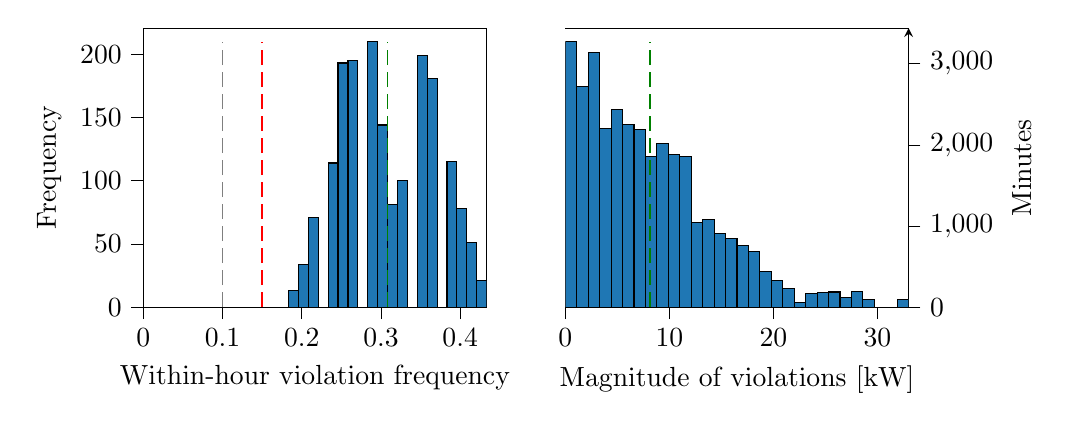
\begin{tikzpicture}

\definecolor{darkgray176}{RGB}{176,176,176}
\definecolor{green}{RGB}{0,128,0}
\definecolor{lightgray204}{RGB}{204,204,204}
\definecolor{steelblue31119180}{RGB}{31,119,180}

\begin{groupplot}[group style={group size=2 by 1}]
\nextgroupplot[
legend cell align={left},
legend style={fill opacity=0.8, draw opacity=1, text opacity=1, draw=lightgray204},
tick align=outside,
tick pos=left,
width=0.49\textwidth,
x grid style={darkgray176},
xlabel={Within-hour violation frequency},
xmin=0, xmax=0.433333333333333,
xtick style={color=black},
y grid style={darkgray176},
ylabel={Frequency},
ymin=0, ymax=220.5,
ytick style={color=black}
]
\draw[draw=black,fill=steelblue31119180] (axis cs:0.183333333333333,0) rectangle (axis cs:0.195833333333333,13);
\draw[draw=black,fill=steelblue31119180] (axis cs:0.195833333333333,0) rectangle (axis cs:0.208333333333333,34);
\draw[draw=black,fill=steelblue31119180] (axis cs:0.208333333333333,0) rectangle (axis cs:0.220833333333333,71);
\draw[draw=black,fill=steelblue31119180] (axis cs:0.220833333333333,0) rectangle (axis cs:0.233333333333333,0);
\draw[draw=black,fill=steelblue31119180] (axis cs:0.233333333333333,0) rectangle (axis cs:0.245833333333333,114);
\draw[draw=black,fill=steelblue31119180] (axis cs:0.245833333333333,0) rectangle (axis cs:0.258333333333333,193);
\draw[draw=black,fill=steelblue31119180] (axis cs:0.258333333333333,0) rectangle (axis cs:0.270833333333333,195);
\draw[draw=black,fill=steelblue31119180] (axis cs:0.270833333333333,0) rectangle (axis cs:0.283333333333333,0);
\draw[draw=black,fill=steelblue31119180] (axis cs:0.283333333333333,0) rectangle (axis cs:0.295833333333333,210);
\draw[draw=black,fill=steelblue31119180] (axis cs:0.295833333333333,0) rectangle (axis cs:0.308333333333333,144);
\draw[draw=black,fill=steelblue31119180] (axis cs:0.308333333333333,0) rectangle (axis cs:0.320833333333333,81);
\draw[draw=black,fill=steelblue31119180] (axis cs:0.320833333333333,0) rectangle (axis cs:0.333333333333333,100);
\draw[draw=black,fill=steelblue31119180] (axis cs:0.333333333333333,0) rectangle (axis cs:0.345833333333333,0);
\draw[draw=black,fill=steelblue31119180] (axis cs:0.345833333333333,0) rectangle (axis cs:0.358333333333333,199);
\draw[draw=black,fill=steelblue31119180] (axis cs:0.358333333333333,0) rectangle (axis cs:0.370833333333333,181);
\draw[draw=black,fill=steelblue31119180] (axis cs:0.370833333333333,0) rectangle (axis cs:0.383333333333333,0);
\draw[draw=black,fill=steelblue31119180] (axis cs:0.383333333333333,0) rectangle (axis cs:0.395833333333333,115);
\draw[draw=black,fill=steelblue31119180] (axis cs:0.395833333333333,0) rectangle (axis cs:0.408333333333333,78);
\draw[draw=black,fill=steelblue31119180] (axis cs:0.408333333333333,0) rectangle (axis cs:0.420833333333333,51);
\draw[draw=black,fill=steelblue31119180] (axis cs:0.420833333333333,0) rectangle (axis cs:0.433333333333333,21);
\path [draw=green, semithick, dash pattern=on 5.55pt off 2.4pt]
(axis cs:0.308194444444444,0)
--(axis cs:0.308194444444444,210);

\path [draw=black, draw opacity=0.5, semithick, dash pattern=on 5.55pt off 2.4pt]
(axis cs:0.1,0)
--(axis cs:0.1,210);

\path [draw=red, semithick, dash pattern=on 5.55pt off 2.4pt]
(axis cs:0.15,0)
--(axis cs:0.15,210);


\nextgroupplot[
axis y line=right,
legend cell align={left},
legend style={fill opacity=0.8, draw opacity=1, text opacity=1, draw=lightgray204},
tick align=outside,
width=0.49\textwidth,
x grid style={darkgray176},
xlabel={Magnitude of violations [kW]},
xmin=0, xmax=32.9949353280271,
xtick pos=left,
xtick style={color=black},
y grid style={darkgray176},
ylabel={Minutes},
ymin=0, ymax=3435.6,
ytick pos=right,
ytick style={color=black},
yticklabel style={anchor=west}
]
\draw[draw=black,fill=steelblue31119180] (axis cs:0.00782494908742126,0) rectangle (axis cs:1.10739529505208,3272);
\draw[draw=black,fill=steelblue31119180] (axis cs:1.10739529505208,0) rectangle (axis cs:2.20696564101673,2722);
\draw[draw=black,fill=steelblue31119180] (axis cs:2.20696564101673,0) rectangle (axis cs:3.30653598698139,3136);
\draw[draw=black,fill=steelblue31119180] (axis cs:3.30653598698139,0) rectangle (axis cs:4.40610633294604,2204);
\draw[draw=black,fill=steelblue31119180] (axis cs:4.40610633294604,0) rectangle (axis cs:5.5056766789107,2440);
\draw[draw=black,fill=steelblue31119180] (axis cs:5.5056766789107,0) rectangle (axis cs:6.60524702487535,2251);
\draw[draw=black,fill=steelblue31119180] (axis cs:6.60524702487535,0) rectangle (axis cs:7.70481737084001,2190);
\draw[draw=black,fill=steelblue31119180] (axis cs:7.70481737084001,0) rectangle (axis cs:8.80438771680467,1857);
\draw[draw=black,fill=steelblue31119180] (axis cs:8.80438771680466,0) rectangle (axis cs:9.90395806276932,2017);
\draw[draw=black,fill=steelblue31119180] (axis cs:9.90395806276932,0) rectangle (axis cs:11.003528408734,1884);
\draw[draw=black,fill=steelblue31119180] (axis cs:11.003528408734,0) rectangle (axis cs:12.1030987546986,1856);
\draw[draw=black,fill=steelblue31119180] (axis cs:12.1030987546986,0) rectangle (axis cs:13.2026691006633,1047);
\draw[draw=black,fill=steelblue31119180] (axis cs:13.2026691006633,0) rectangle (axis cs:14.3022394466279,1080);
\draw[draw=black,fill=steelblue31119180] (axis cs:14.3022394466279,0) rectangle (axis cs:15.4018097925926,913);
\draw[draw=black,fill=steelblue31119180] (axis cs:15.4018097925926,0) rectangle (axis cs:16.5013801385573,846);
\draw[draw=black,fill=steelblue31119180] (axis cs:16.5013801385573,0) rectangle (axis cs:17.6009504845219,760);
\draw[draw=black,fill=steelblue31119180] (axis cs:17.6009504845219,0) rectangle (axis cs:18.7005208304866,691);
\draw[draw=black,fill=steelblue31119180] (axis cs:18.7005208304866,0) rectangle (axis cs:19.8000911764512,444);
\draw[draw=black,fill=steelblue31119180] (axis cs:19.8000911764512,0) rectangle (axis cs:20.8996615224159,330);
\draw[draw=black,fill=steelblue31119180] (axis cs:20.8996615224159,0) rectangle (axis cs:21.9992318683805,235);
\draw[draw=black,fill=steelblue31119180] (axis cs:21.9992318683805,0) rectangle (axis cs:23.0988022143452,59);
\draw[draw=black,fill=steelblue31119180] (axis cs:23.0988022143452,0) rectangle (axis cs:24.1983725603098,170);
\draw[draw=black,fill=steelblue31119180] (axis cs:24.1983725603098,0) rectangle (axis cs:25.2979429062745,184);
\draw[draw=black,fill=steelblue31119180] (axis cs:25.2979429062745,0) rectangle (axis cs:26.3975132522392,187);
\draw[draw=black,fill=steelblue31119180] (axis cs:26.3975132522392,0) rectangle (axis cs:27.4970835982038,120);
\draw[draw=black,fill=steelblue31119180] (axis cs:27.4970835982038,0) rectangle (axis cs:28.5966539441685,196);
\draw[draw=black,fill=steelblue31119180] (axis cs:28.5966539441685,0) rectangle (axis cs:29.6962242901331,97);
\draw[draw=black,fill=steelblue31119180] (axis cs:29.6962242901331,0) rectangle (axis cs:30.7957946360978,0);
\draw[draw=black,fill=steelblue31119180] (axis cs:30.7957946360978,0) rectangle (axis cs:31.8953649820624,0);
\draw[draw=black,fill=steelblue31119180] (axis cs:31.8953649820624,0) rectangle (axis cs:32.9949353280271,97);
\path [draw=green, semithick, dash pattern=on 5.55pt off 2.4pt]
(axis cs:8.10868296789308,0)
--(axis cs:8.10868296789308,3272);

\end{groupplot}

\end{tikzpicture}

%     \includegraphics[width=0.99\columnwidth]{figures/drjcc_oos_histograms_ALSO-X.png}
%     \caption{.}
% \end{figure}

% \begin{figure}[!t]
%     \centering
%     % % This file was created with tikzplotlib v0.10.1.
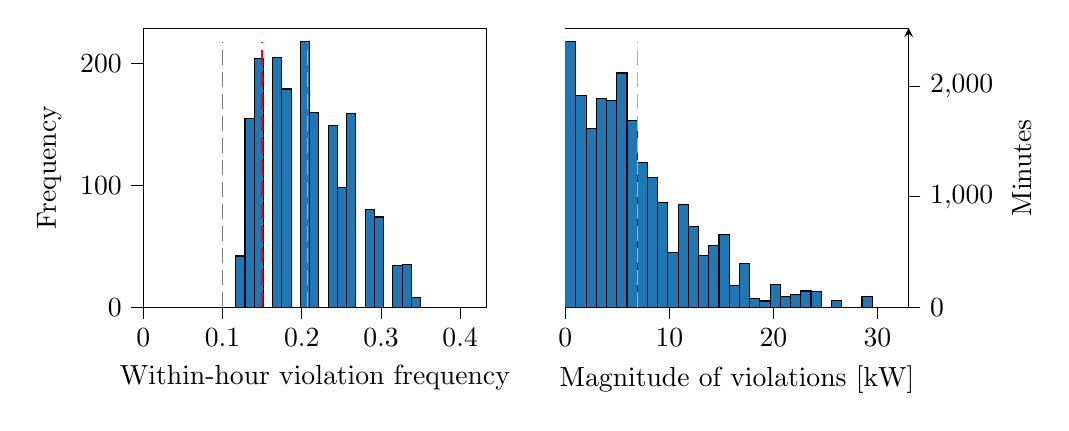
\begin{tikzpicture}

\definecolor{darkgray176}{RGB}{176,176,176}
\definecolor{lightgray204}{RGB}{204,204,204}
\definecolor{orange}{RGB}{255,165,0}
\definecolor{steelblue31119180}{RGB}{31,119,180}

\begin{groupplot}[group style={group size=2 by 1}]
\nextgroupplot[
legend cell align={left},
legend style={fill opacity=0.8, draw opacity=1, text opacity=1, draw=lightgray204},
tick align=outside,
tick pos=left,
width=0.49\textwidth,
x grid style={darkgray176},
xlabel={Within-hour violation frequency},
xmin=0, xmax=0.433333333333333,
xtick style={color=black},
y grid style={darkgray176},
ylabel={Frequency},
ymin=0, ymax=228.9,
ytick style={color=black}
]
\draw[draw=black,fill=steelblue31119180] (axis cs:0.116666666666667,0) rectangle (axis cs:0.128333333333333,42);
\draw[draw=black,fill=steelblue31119180] (axis cs:0.128333333333333,0) rectangle (axis cs:0.14,155);
\draw[draw=black,fill=steelblue31119180] (axis cs:0.14,0) rectangle (axis cs:0.151666666666667,204);
\draw[draw=black,fill=steelblue31119180] (axis cs:0.151666666666667,0) rectangle (axis cs:0.163333333333333,0);
\draw[draw=black,fill=steelblue31119180] (axis cs:0.163333333333333,0) rectangle (axis cs:0.175,205);
\draw[draw=black,fill=steelblue31119180] (axis cs:0.175,0) rectangle (axis cs:0.186666666666667,179);
\draw[draw=black,fill=steelblue31119180] (axis cs:0.186666666666667,0) rectangle (axis cs:0.198333333333333,0);
\draw[draw=black,fill=steelblue31119180] (axis cs:0.198333333333333,0) rectangle (axis cs:0.21,218);
\draw[draw=black,fill=steelblue31119180] (axis cs:0.21,0) rectangle (axis cs:0.221666666666667,160);
\draw[draw=black,fill=steelblue31119180] (axis cs:0.221666666666667,0) rectangle (axis cs:0.233333333333333,0);
\draw[draw=black,fill=steelblue31119180] (axis cs:0.233333333333333,0) rectangle (axis cs:0.245,149);
\draw[draw=black,fill=steelblue31119180] (axis cs:0.245,0) rectangle (axis cs:0.256666666666667,98);
\draw[draw=black,fill=steelblue31119180] (axis cs:0.256666666666667,0) rectangle (axis cs:0.268333333333333,159);
\draw[draw=black,fill=steelblue31119180] (axis cs:0.268333333333333,0) rectangle (axis cs:0.28,0);
\draw[draw=black,fill=steelblue31119180] (axis cs:0.28,0) rectangle (axis cs:0.291666666666667,80);
\draw[draw=black,fill=steelblue31119180] (axis cs:0.291666666666667,0) rectangle (axis cs:0.303333333333333,74);
\draw[draw=black,fill=steelblue31119180] (axis cs:0.303333333333333,0) rectangle (axis cs:0.315,0);
\draw[draw=black,fill=steelblue31119180] (axis cs:0.315,0) rectangle (axis cs:0.326666666666667,34);
\draw[draw=black,fill=steelblue31119180] (axis cs:0.326666666666667,0) rectangle (axis cs:0.338333333333333,35);
\draw[draw=black,fill=steelblue31119180] (axis cs:0.338333333333333,0) rectangle (axis cs:0.35,8);
\path [draw=orange, semithick, dash pattern=on 5.55pt off 2.4pt]
(axis cs:0.207324074074074,0)
--(axis cs:0.207324074074074,218);

\path [draw=black, draw opacity=0.5, semithick, dash pattern=on 5.55pt off 2.4pt]
(axis cs:0.1,0)
--(axis cs:0.1,218);

\path [draw=red, semithick, dash pattern=on 5.55pt off 2.4pt]
(axis cs:0.15,0)
--(axis cs:0.15,218);


\nextgroupplot[
axis y line=right,
legend cell align={left},
legend style={fill opacity=0.8, draw opacity=1, text opacity=1, draw=lightgray204},
tick align=outside,
width=0.49\textwidth,
x grid style={darkgray176},
xlabel={Magnitude of violations [kW]},
xmin=0, xmax=32.9949353280271,
xtick pos=left,
xtick style={color=black},
y grid style={darkgray176},
ylabel={Minutes},
ymin=0, ymax=2526.3,
ytick pos=right,
ytick style={color=black},
yticklabel style={anchor=west}
]
\draw[draw=black,fill=steelblue31119180] (axis cs:0.0387024932025,0) rectangle (axis cs:1.02072485741103,2406);
\draw[draw=black,fill=steelblue31119180] (axis cs:1.02072485741103,0) rectangle (axis cs:2.00274722161957,1915);
\draw[draw=black,fill=steelblue31119180] (axis cs:2.00274722161957,0) rectangle (axis cs:2.9847695858281,1618);
\draw[draw=black,fill=steelblue31119180] (axis cs:2.9847695858281,0) rectangle (axis cs:3.96679195003664,1891);
\draw[draw=black,fill=steelblue31119180] (axis cs:3.96679195003664,0) rectangle (axis cs:4.94881431424517,1873);
\draw[draw=black,fill=steelblue31119180] (axis cs:4.94881431424517,0) rectangle (axis cs:5.93083667845371,2121);
\draw[draw=black,fill=steelblue31119180] (axis cs:5.93083667845371,0) rectangle (axis cs:6.91285904266224,1687);
\draw[draw=black,fill=steelblue31119180] (axis cs:6.91285904266224,0) rectangle (axis cs:7.89488140687078,1313);
\draw[draw=black,fill=steelblue31119180] (axis cs:7.89488140687078,0) rectangle (axis cs:8.87690377107931,1174);
\draw[draw=black,fill=steelblue31119180] (axis cs:8.87690377107931,0) rectangle (axis cs:9.85892613528785,948);
\draw[draw=black,fill=steelblue31119180] (axis cs:9.85892613528785,0) rectangle (axis cs:10.8409484994964,494);
\draw[draw=black,fill=steelblue31119180] (axis cs:10.8409484994964,0) rectangle (axis cs:11.8229708637049,934);
\draw[draw=black,fill=steelblue31119180] (axis cs:11.8229708637049,0) rectangle (axis cs:12.8049932279134,733);
\draw[draw=black,fill=steelblue31119180] (axis cs:12.8049932279134,0) rectangle (axis cs:13.787015592122,470);
\draw[draw=black,fill=steelblue31119180] (axis cs:13.787015592122,0) rectangle (axis cs:14.7690379563305,562);
\draw[draw=black,fill=steelblue31119180] (axis cs:14.7690379563305,0) rectangle (axis cs:15.7510603205391,658);
\draw[draw=black,fill=steelblue31119180] (axis cs:15.7510603205391,0) rectangle (axis cs:16.7330826847476,196);
\draw[draw=black,fill=steelblue31119180] (axis cs:16.7330826847476,0) rectangle (axis cs:17.7151050489561,398);
\draw[draw=black,fill=steelblue31119180] (axis cs:17.7151050489561,0) rectangle (axis cs:18.6971274131647,78);
\draw[draw=black,fill=steelblue31119180] (axis cs:18.6971274131647,0) rectangle (axis cs:19.6791497773732,56);
\draw[draw=black,fill=steelblue31119180] (axis cs:19.6791497773732,0) rectangle (axis cs:20.6611721415817,209);
\draw[draw=black,fill=steelblue31119180] (axis cs:20.6611721415817,0) rectangle (axis cs:21.6431945057903,95);
\draw[draw=black,fill=steelblue31119180] (axis cs:21.6431945057903,0) rectangle (axis cs:22.6252168699988,114);
\draw[draw=black,fill=steelblue31119180] (axis cs:22.6252168699988,0) rectangle (axis cs:23.6072392342073,147);
\draw[draw=black,fill=steelblue31119180] (axis cs:23.6072392342073,0) rectangle (axis cs:24.5892615984159,145);
\draw[draw=black,fill=steelblue31119180] (axis cs:24.5892615984159,0) rectangle (axis cs:25.5712839626244,0);
\draw[draw=black,fill=steelblue31119180] (axis cs:25.5712839626244,0) rectangle (axis cs:26.5533063268329,59);
\draw[draw=black,fill=steelblue31119180] (axis cs:26.5533063268329,0) rectangle (axis cs:27.5353286910415,0);
\draw[draw=black,fill=steelblue31119180] (axis cs:27.5353286910415,0) rectangle (axis cs:28.51735105525,0);
\draw[draw=black,fill=steelblue31119180] (axis cs:28.51735105525,0) rectangle (axis cs:29.4993734194585,97);
\path [draw=orange, semithick, dash pattern=on 5.55pt off 2.4pt]
(axis cs:6.95181103439593,0)
--(axis cs:6.95181103439593,2406);

\end{groupplot}

\end{tikzpicture}

%     \includegraphics[width=0.99\columnwidth]{figures/drjcc_oos_histograms_CVaR.png}
%     \caption{.}
% \end{figure}

% \begin{figure}[!t]
%     \centering
%     % % This file was created with tikzplotlib v0.10.1.
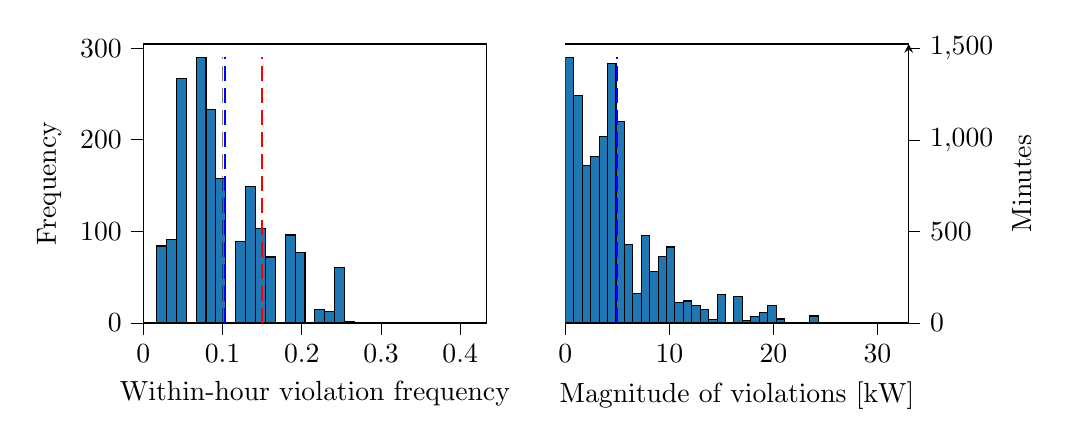
\begin{tikzpicture}

\definecolor{darkgray176}{RGB}{176,176,176}
\definecolor{lightgray204}{RGB}{204,204,204}
\definecolor{steelblue31119180}{RGB}{31,119,180}

\begin{groupplot}[group style={group size=2 by 1}]
\nextgroupplot[
legend cell align={left},
legend style={fill opacity=0.8, draw opacity=1, text opacity=1, draw=lightgray204},
tick align=outside,
tick pos=left,
width=0.49\textwidth,
x grid style={darkgray176},
xlabel={Within-hour violation frequency},
xmin=0, xmax=0.433333333333333,
xtick style={color=black},
y grid style={darkgray176},
ylabel={Frequency},
ymin=0, ymax=304.5,
ytick style={color=black}
]
\draw[draw=black,fill=steelblue31119180] (axis cs:0.0166666666666667,0) rectangle (axis cs:0.0291666666666667,84);
\draw[draw=black,fill=steelblue31119180] (axis cs:0.0291666666666667,0) rectangle (axis cs:0.0416666666666667,91);
\draw[draw=black,fill=steelblue31119180] (axis cs:0.0416666666666667,0) rectangle (axis cs:0.0541666666666667,267);
\draw[draw=black,fill=steelblue31119180] (axis cs:0.0541666666666667,0) rectangle (axis cs:0.0666666666666667,0);
\draw[draw=black,fill=steelblue31119180] (axis cs:0.0666666666666667,0) rectangle (axis cs:0.0791666666666666,290);
\draw[draw=black,fill=steelblue31119180] (axis cs:0.0791666666666667,0) rectangle (axis cs:0.0916666666666667,233);
\draw[draw=black,fill=steelblue31119180] (axis cs:0.0916666666666667,0) rectangle (axis cs:0.104166666666667,158);
\draw[draw=black,fill=steelblue31119180] (axis cs:0.104166666666667,0) rectangle (axis cs:0.116666666666667,0);
\draw[draw=black,fill=steelblue31119180] (axis cs:0.116666666666667,0) rectangle (axis cs:0.129166666666667,89);
\draw[draw=black,fill=steelblue31119180] (axis cs:0.129166666666667,0) rectangle (axis cs:0.141666666666667,149);
\draw[draw=black,fill=steelblue31119180] (axis cs:0.141666666666667,0) rectangle (axis cs:0.154166666666667,103);
\draw[draw=black,fill=steelblue31119180] (axis cs:0.154166666666667,0) rectangle (axis cs:0.166666666666667,72);
\draw[draw=black,fill=steelblue31119180] (axis cs:0.166666666666667,0) rectangle (axis cs:0.179166666666667,0);
\draw[draw=black,fill=steelblue31119180] (axis cs:0.179166666666667,0) rectangle (axis cs:0.191666666666667,96);
\draw[draw=black,fill=steelblue31119180] (axis cs:0.191666666666667,0) rectangle (axis cs:0.204166666666667,77);
\draw[draw=black,fill=steelblue31119180] (axis cs:0.204166666666667,0) rectangle (axis cs:0.216666666666667,0);
\draw[draw=black,fill=steelblue31119180] (axis cs:0.216666666666667,0) rectangle (axis cs:0.229166666666667,15);
\draw[draw=black,fill=steelblue31119180] (axis cs:0.229166666666667,0) rectangle (axis cs:0.241666666666667,13);
\draw[draw=black,fill=steelblue31119180] (axis cs:0.241666666666667,0) rectangle (axis cs:0.254166666666667,61);
\draw[draw=black,fill=steelblue31119180] (axis cs:0.254166666666667,0) rectangle (axis cs:0.266666666666667,2);
\path [draw=blue, semithick, dash pattern=on 5.55pt off 2.4pt]
(axis cs:0.102833333333333,0)
--(axis cs:0.102833333333333,290);

\path [draw=black, draw opacity=0.5, semithick, dash pattern=on 5.55pt off 2.4pt]
(axis cs:0.1,0)
--(axis cs:0.1,290);

\path [draw=red, semithick, dash pattern=on 5.55pt off 2.4pt]
(axis cs:0.15,0)
--(axis cs:0.15,290);


\nextgroupplot[
axis y line=right,
legend cell align={left},
legend style={fill opacity=0.8, draw opacity=1, text opacity=1, draw=lightgray204},
tick align=outside,
width=0.49\textwidth,
x grid style={darkgray176},
xlabel={Magnitude of violations [kW]},
xmin=0, xmax=32.9949353280271,
xtick pos=left,
xtick style={color=black},
y grid style={darkgray176},
ylabel={Minutes},
ymin=0, ymax=1524.6,
ytick pos=right,
ytick style={color=black},
yticklabel style={anchor=west}
]
\draw[draw=black,fill=steelblue31119180] (axis cs:0.00773765166348278,0) rectangle (axis cs:0.817551882640649,1452);
\draw[draw=black,fill=steelblue31119180] (axis cs:0.817551882640649,0) rectangle (axis cs:1.62736611361782,1245);
\draw[draw=black,fill=steelblue31119180] (axis cs:1.62736611361782,0) rectangle (axis cs:2.43718034459498,861);
\draw[draw=black,fill=steelblue31119180] (axis cs:2.43718034459498,0) rectangle (axis cs:3.24699457557215,911);
\draw[draw=black,fill=steelblue31119180] (axis cs:3.24699457557215,0) rectangle (axis cs:4.05680880654931,1017);
\draw[draw=black,fill=steelblue31119180] (axis cs:4.05680880654931,0) rectangle (axis cs:4.86662303752648,1416);
\draw[draw=black,fill=steelblue31119180] (axis cs:4.86662303752648,0) rectangle (axis cs:5.67643726850365,1099);
\draw[draw=black,fill=steelblue31119180] (axis cs:5.67643726850365,0) rectangle (axis cs:6.48625149948081,427);
\draw[draw=black,fill=steelblue31119180] (axis cs:6.48625149948081,0) rectangle (axis cs:7.29606573045798,163);
\draw[draw=black,fill=steelblue31119180] (axis cs:7.29606573045798,0) rectangle (axis cs:8.10587996143514,480);
\draw[draw=black,fill=steelblue31119180] (axis cs:8.10587996143514,0) rectangle (axis cs:8.91569419241231,282);
\draw[draw=black,fill=steelblue31119180] (axis cs:8.91569419241231,0) rectangle (axis cs:9.72550842338948,363);
\draw[draw=black,fill=steelblue31119180] (axis cs:9.72550842338948,0) rectangle (axis cs:10.5353226543666,415);
\draw[draw=black,fill=steelblue31119180] (axis cs:10.5353226543666,0) rectangle (axis cs:11.3451368853438,110);
\draw[draw=black,fill=steelblue31119180] (axis cs:11.3451368853438,0) rectangle (axis cs:12.154951116321,120);
\draw[draw=black,fill=steelblue31119180] (axis cs:12.154951116321,0) rectangle (axis cs:12.9647653472981,94);
\draw[draw=black,fill=steelblue31119180] (axis cs:12.9647653472981,0) rectangle (axis cs:13.7745795782753,72);
\draw[draw=black,fill=steelblue31119180] (axis cs:13.7745795782753,0) rectangle (axis cs:14.5843938092525,21);
\draw[draw=black,fill=steelblue31119180] (axis cs:14.5843938092525,0) rectangle (axis cs:15.3942080402296,156);
\draw[draw=black,fill=steelblue31119180] (axis cs:15.3942080402296,0) rectangle (axis cs:16.2040222712068,0);
\draw[draw=black,fill=steelblue31119180] (axis cs:16.2040222712068,0) rectangle (axis cs:17.013836502184,144);
\draw[draw=black,fill=steelblue31119180] (axis cs:17.013836502184,0) rectangle (axis cs:17.8236507331611,12);
\draw[draw=black,fill=steelblue31119180] (axis cs:17.8236507331611,0) rectangle (axis cs:18.6334649641383,34);
\draw[draw=black,fill=steelblue31119180] (axis cs:18.6334649641383,0) rectangle (axis cs:19.4432791951155,55);
\draw[draw=black,fill=steelblue31119180] (axis cs:19.4432791951155,0) rectangle (axis cs:20.2530934260926,96);
\draw[draw=black,fill=steelblue31119180] (axis cs:20.2530934260926,0) rectangle (axis cs:21.0629076570698,22);
\draw[draw=black,fill=steelblue31119180] (axis cs:21.0629076570698,0) rectangle (axis cs:21.872721888047,1);
\draw[draw=black,fill=steelblue31119180] (axis cs:21.872721888047,0) rectangle (axis cs:22.6825361190241,0);
\draw[draw=black,fill=steelblue31119180] (axis cs:22.6825361190241,0) rectangle (axis cs:23.4923503500013,0);
\draw[draw=black,fill=steelblue31119180] (axis cs:23.4923503500013,0) rectangle (axis cs:24.3021645809785,38);
\path [draw=blue, semithick, dash pattern=on 5.55pt off 2.4pt]
(axis cs:4.93759148683224,0)
--(axis cs:4.93759148683224,1452);

\end{groupplot}

\end{tikzpicture}

%     \includegraphics[width=0.99\columnwidth]{figures/drjcc_oos_histograms_DRJCC.png}
%     \caption{.}
% \end{figure}

% Write something

% \begin{figure}[!t]
%     \centering
%     % \input{figures/heatmap.tikz} % OBS: does not work
%     \includegraphics[width=0.99\columnwidth]{figures/heatmap.png}
%     \caption{.}
% \end{figure}

\clearpage
\newpage


\section*{Equations}

\noindent Sets:

\begin{itemize}
    \item $\mathcal{H} = \{1, 2,  \ldots 24\}$
    \item $\mathcal{M} = \{1, 2,  \ldots 1440\}$
    \item $ \mathcal{M}_{h} = \{h \times 60 + m \mid m \in \{0, 1, 2, \ldots, 59\}\}$
     \item $\mathcal{I} = \{1, 2, \ldots \thinspace \text{Number of samples} \}$

\end{itemize}

\noindent Definitions:

\begin{definition}[Energinet's P90 rule \cite{energinet}]
    This means, that the participant's prognosis, which must be approved by Energinet, evaluates that the probability is 10\% that the sold capacity is not available. This entails that there is a 90\% chance that the sold capacity or more is available. This is when the prognosis is assumed to be correct.

    The probability is then also 10\%, that the entire sold capacity is not available. If this were to happen, it does not entail that the sold capacity is not available at all, however just that a part of the total capacity is not available. The available part will with high probability be close to the sold capacity.
\end{definition}

Simple optimization problem where bids, $p_{h}^{\text{cap}}$, must be adhere to uncertain available flexibility, $P_{m}^{\text{B}}(\xi)$.

\begin{subequations}\label{P90:P1}
    \begin{align}
        \max_{p_{h}^{\text{cap}}} \quad & \sum_h \lambda_h p_{h}^{\text{cap}}                                                                                                                                                                                                     \\
        \text{s.t.} \quad               & \mathbb{P}  \left( p_{h}^{\text{cap}} \leq P_{m}^{\text{B}}(\xi), \quad \forall{m} \in \mathcal{M}_{h},  \forall{h} \in \mathcal{H}  \right) \geq 1 - \epsilon \label{P90:p1:c}
    \end{align}
\end{subequations}

\section*{DRJCC}

Converting \eqref{P90:P1} to DRJCC for distributions within some ambiguity set defined by Wasserstein distance $\theta$:

\begin{subequations}\label{P90:P1:DRJCC}
    \begin{align}
        \max_{p_{h}^{\text{cap}}} \quad & \sum_h \lambda_h p_{h}^{\text{cap}}                                                                                                                                                                                                     \\
        \text{s.t.} \quad               & \mathbb{P}  \left( p_{h}^{\text{cap}} \leq P_{m}^{\text{B}}(\xi), \quad \forall{m} \in \mathcal{M}_{h},  \forall{h} \in \mathcal{H}  \right) \geq 1 - \epsilon \quad \forall{\mathbb{P}} \in \mathcal{F}(\theta) \label{P90:p1:drjcc_c}
    \end{align}
\end{subequations}

A tractable formulation of \eqref{P90:P1:DRJCC} is given by \cite[Proposition 2]{chen2022data}:

\begin{subequations}\label{P90:P1:DRJCC-tract}
\begin{align}
    \max_{p_{h}^{\text{cap}}, q_i, s_i \geq 0, t} \quad & \sum_h \lambda_h p_{h}^{\text{cap}}                                                                                                                                    \\
    \text{s.t.} \quad                                   & \epsilon |\mathcal{I}| t - \sum_{i \in \mathcal{I}} s_i \geq \theta |\mathcal{I}|                                                                                      \\
                                                        & P_{m}^{\text{B}}(\xi_i) - p_{h}^{\text{cap}} + M\cdot q_i \geq t - s_i, \quad \forall{m} \in \mathcal{M}_{h},  \forall{h} \in \mathcal{H},  \forall{i} \in \mathcal{I} \\
                                                        & M (1-q_i) \geq t - s_i                                                                                                                                                 \\
                                                        & q_i \in \{0,1 \}, \quad \forall{i} \in \mathcal{I}
\end{align}
\end{subequations}


Let the set of flexible demands be denoted by $d \in \{\mathcal{D} \}$. Then TSO profit is described by the following bi-level problem:

\begin{subequations}
    \begin{align}
        \max_{\epsilon, \theta} \quad & \sum_h \lambda_h p_{h,d}^{\text{cap}} - \sum_h \sum_d \frac{1}{|\mathcal{I}|}\sum_i \nu_{h,i,d}                                                                                                                                                                                                      \\
        \text{s.t.} \quad               & \text{Problem} \thinspace \eqref{P90:P1:DRJCC-tract}, \quad \forall{d} \\
        & \nu_{h,i,d} = \left(p_{h,d}^{\text{cap}} - P_{m}^{\text{B}}(\xi_i) \right)^{+}, \quad \forall{i}, \forall{h}, \forall{d}
    \end{align}
\end{subequations}

\section*{ALSO-X}

Inspired by \cite{jiang2022also, porras2023integrating}, the reformulation of \eqref{P90:P1} is:

\begin{align}\label{P90:P1:ALSO-X}
    \max_{p_{h}^{\text{cap}}, y_{m,i} } \quad & \sum_h \lambda_h p_{h}^{\text{cap}}                                                                                                                                            \\
    \text{s.t.} \quad                         & -(1-y_{m,i})M \leq  p_{h}^{\text{cap}} - P_{m}^{\text{B}}(\xi_i) \leq y_{m,i} M, \quad \forall{m} \in \mathcal{M}_{h},  \forall{h} \in \mathcal{H}, \forall{i} \in \mathcal{I} \\
                                              & \sum_{i \in \mathcal{I}, m \in \mathcal{H}} y_{m,i} \leq q                                                                                                                     \\
                                              & y_{m,i} \in \{0,1\}, \quad \forall{m} \in \mathcal{M}_{h},  \forall{h} \in \mathcal{H}, \forall{i} \in \mathcal{I}
\end{align}

Here, $q = \lfloor  \epsilon \cdot |\mathcal{I}|  \cdot |\mathcal{M}| \rfloor $ and $y_{m,i}$ is a binary variable indicating an overbid in minute $m$ and sample $i$. The ALSO-X algorithm as listed in Algorithm \ref{alg:also_x} iteratively conducts an exponential search for the best value of $q$ such that the frequency of violations is less than $\epsilon$ by solving a relaxed version of \eqref{P90:P1:ALSO-X} with respect to $y_{m,i}$. Thus, ALSO-X does not consider the magnitude of violation - as opposed to CVaR - but only the frequency of violations. It is therefore expected that ALSO-X is less conservative than CVaR which was also the motivation behind its incarnation \cite{jiang2022also}.

\begin{algorithm}
    \caption{ALSO-X}
    \label{alg:also_x} % This is the label for referencing
    \begin{algorithmic}[1]
        \Require Relax the integrality of $y$
        Input: Stopping tolerance parameter $ \delta $
        \State$ q \leftarrow 0, \bar{q} \leftarrow \lceil -\epsilon \rceil $
        \While{ $ q \neq \bar{q} $ }
        \State Set $ q_a \leftarrow (q + \bar{q})/2 $ and retrieve $ \Theta^* $ as an optimal solution to $ (4) $.
        \State Set $ q \leftarrow q_a $ if $ P(y^* = 0) \geq 1 - \epsilon $; otherwise, $ \bar{q} \leftarrow q $
        \EndWhile
        Output: A feasible solution of model \eqref{P90:P1:ALSO-X}.
    \end{algorithmic}
\end{algorithm}

\section*{CVaR}

First, let $\mathcal{I}$ denote the number of samples for the empirical distribution. The CVaR formulation of the JCC in \eqref{P90:P1} is then \cite{jiang2022also}:

\begin{align}\label{P90:P1:CVaR}
    \max_{p_{h}^{\text{cap}}, \beta \geq 0, \zeta_{m,i}} \quad & \sum_h \lambda_h p_{h}^{\text{cap}}                                                                                                                          \\
    \text{s.t.} \quad                                          & p_{h}^{\text{cap}} - P_{m}^{\text{B}}(\xi_i) \leq \zeta_{m,i}, \quad \forall{m} \in \mathcal{M}_{h},  \forall{h} \in \mathcal{H}, \forall{i} \in \mathcal{I} \\
                                                               & \frac{1}{|\mathcal{M}|\cdot |\mathcal{I}|} \sum_{i \in \mathcal{I}, m \in \mathcal{H}} \zeta_{m,i} - (1-\epsilon)\cdot \beta \leq 0                          \\
                                                               & \beta \leq  \zeta_{m,i}, \quad  \forall{m} \in \mathcal{M}_{h},  \forall{h} \in \mathcal{H}, \forall{i} \in \mathcal{I}
\end{align}

The CVaR approximation in \eqref{P90:P1:CVaR} is a simple LP. The JCC is now approximated such that expected value of the $\epsilon$ worst samples and minutes is attenuated.

\printbibliography

\end{document}
